\part{各种心律失常及其心电象}

本篇是本书的重点和难点内容,主要根据心律失常的高发生率(早搏、逸搏、扑动与颤动)、心律失常的发生机制(折返型、自律性增高型、并行心律型及触发活动型)、传导阻滞(文氏现象、心房内传导阻滞、房室传导阻滞、束支与分支阻滞、3相及4相阻滞、传出阻滞、双层及多层阻滞等)及各类专题性内容进行编写,着重阐述了各种心电现象的基本概念、发生机制、心电图特征及临床意义,并配备了大量精彩图例,大部分绘制了梯形图解以帮助读者理解,共32章。

\protect\hypertarget{text00016.html}{}{}

\protect\hypertarget{text00016.htmlux5cux23chapter16}{}{}

\chapter{破解心律失常诊断三步曲}

十二导联同步心电图对心律失常具有独特的诊断价值,大多能明确心律失常发生的部位及其基本性质。为达到正确地分析心律失常之目的,必须做到:①良好的心电图记录;②掌握心律失常分析的步骤及方法;③借助梯形图解进行合乎逻辑的推理和验证;④掌握心律失常诊断的基本原则;⑤密切结合临床及既往心电图改变。

\protect\hypertarget{text00016.htmlux5cux23subid116}{}{}

\subsection{良好的心电图记录}

1.选择最合适的导联

心房波的检出是正确分析心律失常的关键。首选Ⅱ导联或V\textsubscript{1}导联或两者同步记录,次选aVF、V\textsubscript{1}导联,因这些导联能清楚地显示P波、F波及f波,能确定QRS波形是呈左束支阻滞型还是呈右束支阻滞型,有助于判断是心室内差异性传导还是室性早搏,若为后者,是起源于左心室还是起源于右心室。假如P波振幅低小或不很清楚,除加大振幅(定准电压增至2.0mV)外,还可加做以下特殊导联以显示清晰的P波:①S\textsubscript{5}导联:左手导联线(黄色)用吸球吸在胸骨右缘第5肋间作为正极,右手导联线(红色)用吸球吸在胸骨柄处作为负极,描记方法采用Ⅰ导联,S\textsubscript{5}导联所记录的P波较常用的十二个导联的P波要清晰;②心房导联:探查电极置于胸骨右缘第3肋间,无关电极与中心电站相连,如将右手导联线(红色)用吸球吸在上述部位,描记方法采用aVR导联;③A导联:用记录S\textsubscript{5}导联方法,将正极放置在剑突部,负极放置在胸骨柄正中,所描记P波振幅较高且直立;④食道导联:有条件的最好能采用食道导联,以显示清晰的P波。

2.足够长的记录时间

为了找出紊乱心律内在的规律性,需作较长时间的连续记录,使周期性规律至少能重复2~3次以上。

\protect\hypertarget{text00016.htmlux5cux23subid117}{}{}

\subsection{破解心律失常诊断三步曲}

破解心律失常诊断的基本步骤:①寻找明显的P波,找出P波的规律;②确定P波和QRS波群之间的关系;③找出QRS波群的规律。

1.寻找明显的P波,确定基本节律

在分析复杂心律失常时,寻找P波是最关键的一步。当初看一份心电图,未见明显P波时,要特别关注T波的形态,确认有无P波重叠在T波顶峰上。一旦判明P波存在与否,心律失常诊断与鉴别诊断的范围就大为缩小。如果肯定P波存在,则根据其形态、频率、节律及与QRS波群的关系来判断其起源部位。若肯定为窦性P波,应根据其频率、节律,确定有无不齐、过缓、过速,有无窦房传导阻滞及窦性停搏等;根据P波形态确定有无游走、P波电轴左偏、心房肥大、心房内传导阻滞、房性融合波、心房内差异性传导等;若Ⅱ、Ⅲ、aVF导联P波呈负正双相,aVR导联呈正负双相,则可判定为心房内异位节律,根据其频率、节律,确定是阵发性房性心动过速、加速的房性逸搏心律,还是房性逸搏心律等;若为逆行P\textsuperscript{-}波,则根据P\textsuperscript{-}-R间期长短,判定是心房下部节律,还是房室交接区节律,尔后再根据其频率、节律,确定心律失常的基本性质。若同一导联上还存在其他多种P波时,观察它们是提早出现,还是延迟出现,借以确定是早搏,还是逸搏;如为早搏,则需观察其偶联间期是否一致,两异位搏动之间有无倍数关系,借以确定心律失常的发生机制,是折返型、异位兴奋增高型还是并行心律型,是单源性、多源性还是多形性。若P波消失,代之以快速而规律的无等电位线锯齿状波,则为心房扑动;有时心房扑动呈2:1下传,若此时F波重叠在QRS波群或T波中,则极易误诊为窦性心动过速、房性心动过速或室上性心动过速等;若F波频率慢至160次/min,则易误诊为房性心动过速。若P波消失,代之以频率、波幅、间距、形态均不等的无等电位线的杂乱无章f波时,则为心房颤动;有时f波细小到难以辨认,仅根据R-R间期绝对不规则来诊断心房颤动。如果确实无P波,也无F、f波,那么应注意有无高钾血症引起的窦-室传导、窦性停搏、三度窦房传导阻滞及心房静止等较少见的心律失常,有条件的话,最好记录食道导联,以排除P波或P′波是否隐没在QRS波群之中。

2.根据P-R间期固定与否,确定P波与QRS波群之间的关系

在找出P波之后,根据P-R间期或R-P\textsuperscript{-}间期固定与否,确定P波与QRS波群之间有无关系,也是分析心律失常至关重要的一步。

(1)P波与QRS波群有关:①若P波在QRS波群之前,则根据P-R间期长短确定有无短P-R间期、L-G-L综合征、W-P-W综合征及一度房室传导阻滞、房室结内双径路或多径路传导。②若P-R间期逐渐延长直至P波下传受阻QRS波群脱落,则为文氏型房室传导阻滞;若P-R间期固定,有P波下传受阻现象,则为二度Ⅱ型或高度房室传导阻滞,应注意P波下传受阻后有无房室交接性逸搏、室性逸搏出现。③若P\textsuperscript{-}波在QRS波群之前,P\textsuperscript{-}-R间期<0.12s或者P\textsuperscript{-}波在QRS波群之后,R-P\textsuperscript{-}间期<0.16s,QRS波形正常,则为房室交接性心律,应注意有无反复搏动存在。

(2)P波与QRS波群部分无关:二度~高度房室传导阻滞伴下级起搏点被动发放、不完全干扰性房室分离时,可出现P波与QRS波群之间部分无关现象,此时的P-R间期较正常P-R间期短0.05~0.06s以上。

(3)P波与QRS波群完全无关:三度房室传导阻滞、完全性干扰性房室分离时,出现P-R间期长短不一,而R-R间期却固定不变的现象,根据P波及QRS波群频率的快、慢来区分该房室分离是阻滞性所致还是干扰性所致。

3.寻找QRS波群的规律性

(1)若QRS波群均由P波下传,且其形态正常,则应注意有无电轴偏移、异常Q波、心室肥大及ST段、T波、U波改变等情况。

(2)若P波下传的QRS波群宽大畸形,则应判断是束支阻滞、不定型心室内传导阻滞、心室内差异性传导,还是预激综合征或预激综合征合并束支阻滞所致。

(3)若形态正常QRS波群与P波无关,则应注意该QRS波群是提早出现,还是延迟出现,是连续3次以上,还是单个出现。若为提早出现,其偶联间期是否相等,两异位搏动之间有无倍数关系;若为延迟出现,应关注是什么原因引起的。

(4)若宽大畸形QRS波群与P波无关,则要确定该QRS波群是起源于房室交接区伴束支阻滞,还是起源于心室。是提早出现,还是延迟出现,若为延迟出现,是什么原因引起的。

(5)若心房扑动、心房颤动时出现宽大畸形QRS波群,则要确定该QRS波群是室性早搏还是心室内差异性传导、间歇性束支阻滞或预激综合征;若连续3次以上,则要确定是室性心动过速、心室内差异性传导还是束支阻滞或预激综合征。

(6)若出现窄QRS、宽QRS心动过速,则应按第三十一、三十二章有关方法进行诊断和鉴别诊断。

(7)若遇及长R-R间歇,则要注意T波上有无P′波重叠而呈阻滞型房性早搏,注意有无窦性停搏、窦房传导阻滞、房室传导阻滞及节律重整、隐匿性传导等各种心电现象。

\protect\hypertarget{text00016.htmlux5cux23subid118}{}{}

\subsection{借助梯形图解进行验证}

通过以上分析,一般的心律失常大多能得到正确的诊断,但疑难复杂的心律失常,必须借助梯形图解进行合乎逻辑的推理和验证,使心律失常起源部位、发生机制让人一目了然。绘制梯形图解的方法及要领请见第十章。

\protect\hypertarget{text00016.htmlux5cux23subid119}{}{}

\subsection{诊断心律失常的基本原则}

(1)诊断心律失常时,必须明确起搏点的解剖位置(如窦房结、心房、房室交接区、心室、房室旁道等)、起搏点发放冲动的频率强度(如正常、加速的、过速、过缓、早搏、逸搏、停搏等)、冲动在各个部位的传导情况(如正常、传导阻滞、超常传导、多径路传导、隐匿性传导、差异性传导等)、伴随现象(如早搏诱发反复搏动及反复性心动过速、房性早搏诱发快速性房性心律失常、室性早搏诱发快速性室性心律失常及隐匿性传导、节律重整等)。

(2)诊断心律失常时,尽量用最常见的心律失常发生机制来解释,少用罕见的心律失常发生机制来解释。

(3)诊断心律失常时,尽量用“一元论”来解释,如能用一种心律失常来解释,则不必用多种心律失常来解释,实在难以圆满解释时,可用多种心律失常及其机制来解释。

(4)诊断心律失常时,整幅心电图所见的各种现象,都能得到圆满地解释。

(5)诊断心律失常时,要符合目前公认的各种理论及心电现象,各个诊断之间不能自相矛盾。

(6)诊断心律失常时,必须密切结合临床及电生理检查。

(7)诊断心律失常时,诊断顺序可按起搏点的解剖顺序(如房性早搏、室性早搏等)、传导组织先后顺序等书写(如二度Ⅱ型窦房传导阻滞、一度房室传导阻滞、右束支阻滞等),或先写原发性心律失常,后写继发性心律失常(如三度房室传导阻滞、房室交接性逸搏心律等),或先写严重心律失常,后写次要心律失常。

\protect\hypertarget{text00016.htmlux5cux23subid120}{}{}

\subsection{密切结合临床及既往心电图改变}

诊断心律失常时,必须密切结合临床、既往心电图改变及电生理检查,如宽、窄QRS心动过速的诊断、心房颤动伴心室内差异性传导还是伴室性早搏等。

\protect\hypertarget{text00017.html}{}{}

\protect\hypertarget{text00017.htmlux5cux23chapter17}{}{}

\chapter{破解心律失常诊断的利器------梯形图解}

梯形图解能简明而精确地表达复杂心律失常的发生机制,解释某些特殊的心电现象,如隐匿性传导、空隙现象、折返现象、文氏现象、蝉联现象、超常传导及韦金斯基现象等,使其一目了然。借助梯形图解来判断、证实对某一复杂心律失常的分析、诊断是否正确,同时又能启迪和加深对心律失常的理解,是破解心律失常诊断的利器。此外,食道心电图能判明有无P波及P波与QRS波群之间有无关联,亦是破解心律失常诊断的利器。

\protect\hypertarget{text00017.htmlux5cux23subid121}{}{}

\subsection{绘制梯形图解的原则}

(1)绘制梯形图解之前必须对该心律失常的发生机制有初步的了解,否则,将无从下手。

(2)梯形图解由横线、垂直线及斜线绘制而成。在能说明问题的情况下,愈简单愈好,即横线条、符号和缩写字母愈少,愈简洁明了,通常选用三行图、五行图。

(3)A行内的垂直线代表心房激动,对准P波的起始处,V行内的垂直线代表心室激动,对准QRS波群的起始处。若有S行,则S行内垂直线画在A行垂直线前0.07~0.12s,一般为0.10s,代表窦性激动。

(4)各行宽度视需要而定。一般而言,S行、A行、V行及E行的宽度基本一致且较窄,约0.5cm;S-A行、E-V行略宽,约0.6cm;A-V行较宽约0.7cm,若房室交接区存在双层、三层阻滞,则该行可分别宽至1.0、1.2~1.5cm;RP行最宽可达1.2~1.5cm。图中所标时间的单位为cs(1cs=0.01s)。

(5)如遇窦性或异位节律重整现象,必要时在梯形图上另加符号,说明原来及重整后节律周期的长度,如窦性周期用SC、异位周期用EC、并行心律的最大公约数用数字X倍数来表明,以帮助阅读和理解。

\protect\hypertarget{text00017.htmlux5cux23subid122}{}{}

\subsection{绘制梯形图解常用的缩写字母、符号及意义}

\begin{longtable}{lr}
S代表窦房结&L代表左束支\\
S-A代表窦房交接区&a代表左前分支\\
A代表心房&p代表左后分支\\
A-V代表房室交接区&E代表心房或心室内异位起搏点\\
V代表心室&E-V代表异-室交接区\\
BB代表束支& RP代表心房或心室内折返径路\\
R代表右束支&FB代表房性或室性融合波\\
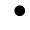
\includegraphics{./images/Image00125.jpg}代表正位或异位起搏点&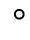
\includegraphics{./images/Image00126.jpg}代表正位或异位预期起搏点\\
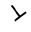
\includegraphics{./images/Image00127.jpg}代表激动顺向传导(前向传导)受阻&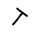
\includegraphics{./images/Image00128.jpg}代表激动逆向传导受阻\\
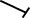
\includegraphics{./images/Image00129.jpg}代表激动顺向隐匿性传导&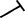
\includegraphics{./images/Image00130.jpg}代表激动逆向隐匿性传导\\
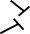
\includegraphics{./images/Image00131.jpg}代表两个不同方向的激动相互干扰&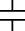
\includegraphics{./images/Image00132.jpg}代表房性或室性融合波\\
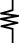
\includegraphics{./images/Image00133.jpg}代表心房或心室内差异性传导&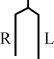
\includegraphics{./images/Image00134.jpg}代表激动通过右束支及左束支\\
\multicolumn{2}{l}{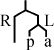
\includegraphics{./images/Image00135.jpg}代表激动通过右束支、左束支及左前分支}\\
\multicolumn{2}{l}{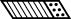
\includegraphics{./images/Image00136.jpg}代表激动顺向传导使传导组织产生的绝对不应期(斜线区)和相对不应期(虚点区)}\\
\multicolumn{2}{l}{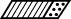
\includegraphics{./images/Image00137.jpg}代表激动逆向传导使传导组织产生的绝对不应期(斜线区)和相对不应期(虚点区)}\\
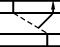
\includegraphics{./images/Image00138.jpg}窦性或房性反复搏动&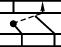
\includegraphics{./images/Image00139.jpg}房室交接性反复搏动\\
\multicolumn{2}{l}{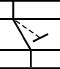
\includegraphics{./images/Image00141.jpg}房室交接区快径路下传、慢径路下传受阻}\\
\multicolumn{2}{l}{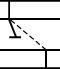
\includegraphics{./images/Image00142.jpg}房室交接区慢径路下传、快径路下传受阻}\\
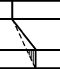
\includegraphics{./images/Image00143.jpg}部分性预激&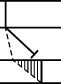
\includegraphics{./images/Image00144.jpg}完全性预激
\end{longtable}

\protect\hypertarget{text00017.htmlux5cux23subid123}{}{}

\subsection{绘制梯形图解常用的格式}

(1)反映窦房结和窦房交接区起搏点、传导及折返情况:选用S、S-A、A三行图(图\ref{fig10-1})。

\begin{figure}[!htbp]
 \centering
 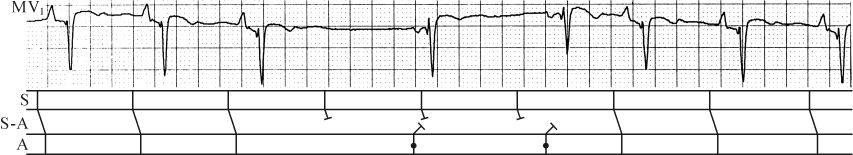
\includegraphics[width=5.76042in,height=1.04167in]{./images/Image00145.jpg}
 \captionsetup{justification=centering}
 \caption{高度窦房传导阻滞、房性逸搏伴不齐或起步现象、房性逸搏揭示窦性并行心律、异常Q波}
 \label{fig10-1}
  \end{figure} 

(2)反映窦房结(或心房)起搏点、房室交接区传导及折返情况:选用A、A-V、V三行图(图\ref{fig10-2})。

\begin{figure}[!htbp]
 \centering
 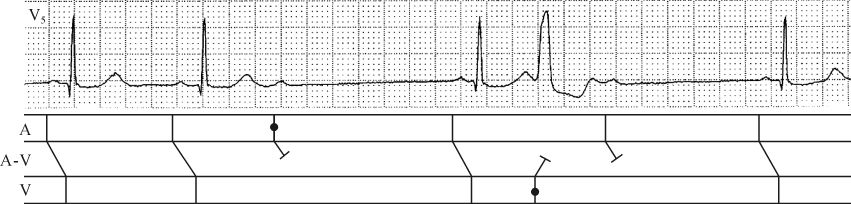
\includegraphics[width=5.75in,height=1.375in]{./images/Image00146.jpg}
 \captionsetup{justification=centering}
 \caption{室相性窦性心律不齐、阻滞型房性早搏及室性早搏揭示3相性二度房室传导阻滞}
 \label{fig10-2}
  \end{figure} 

(3)反映窦房结起搏点、窦房交接区传导、心房起搏点、房室交接区传导及折返情况:选用S、

S-A、A、A-V、V五行图(图\ref{fig10-3})。

\begin{figure}[!htbp]
 \centering
 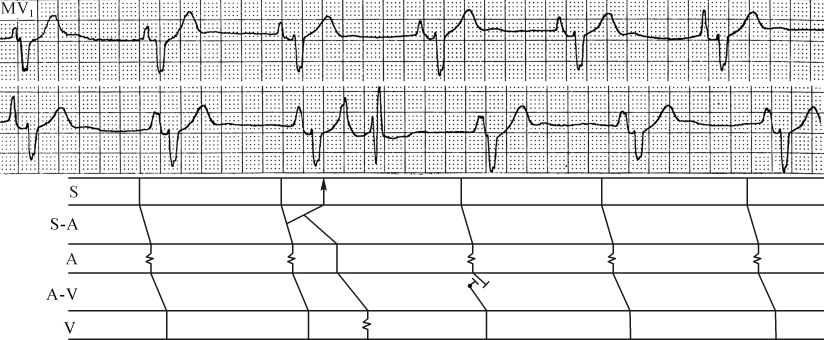
\includegraphics[width=5.5625in,height=2.29167in]{./images/Image00147.jpg}
 \captionsetup{justification=centering}
 \caption{MV\textsubscript{1}导联连续记录,显示窦性心动过缓、文氏型右心房内传导阻滞、不完全性左心房内传导阻滞、窦房交接区折返性早搏伴心室内差异性传导、房室交接性逸搏}
 \label{fig10-3}
  \end{figure} 


(4)反映束支传导情况:选用A、A-V、BB、V四行图(图\ref{fig10-4})。

\begin{figure}[!htbp]
 \centering
 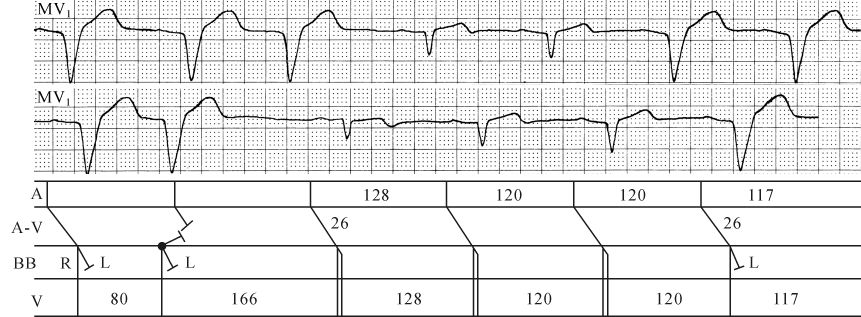
\includegraphics[width=5.82292in,height=2.13542in]{./images/Image00148.jpg}
 \captionsetup{justification=centering}
 \caption{上、下两行系MV\textsubscript{1}导联不同时刻记录,定准电压0.5mV。显示窦性心动过缓、完全性左束支传导阻滞、一度房室传导阻滞(P-R间期0.26s),提示发生在右束支内、房室交接性早搏诱发左束支内韦金斯基现象或揭示3相性左束支传导阻滞}
 \label{fig10-4}
  \end{figure} 


(5)反映心室异位起搏点、异-肌交接区传导及折返情况:选用V、E-V、E三行图(图\ref{fig10-5})。

\begin{figure}[!htbp]
 \centering
 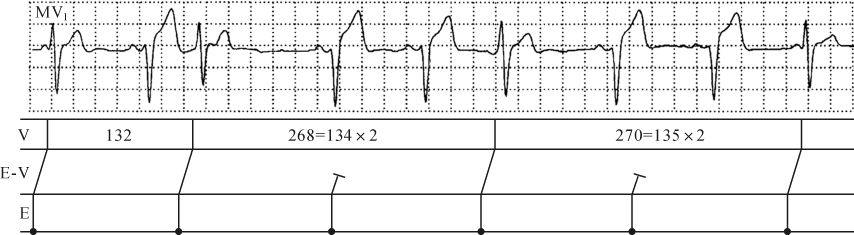
\includegraphics[width=5.77083in,height=1.58333in]{./images/Image00149.jpg}
 \captionsetup{justification=centering}
 \caption{并行性高位室性早搏二、三联律}
 \label{fig10-5}
  \end{figure} 

(6)反映心室折返径路内传导情况:选用V、RP两行图(图\ref{fig10-6})。

\begin{figure}[!htbp]
 \centering
 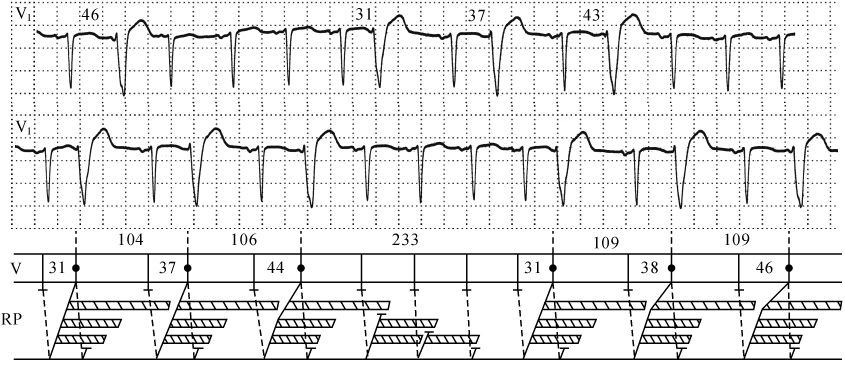
\includegraphics[width=5.70833in,height=2.46875in]{./images/Image00150.jpg}
 \captionsetup{justification=centering}
 \caption{V\textsubscript{1}导联连续记录,显示短阵性室性早搏二联律、心室折返径路内A型交替性文氏周期伴三水平阻滞(近端2:1阻滞、中端呈5:4传导、远端4:3文氏现象)}
 \label{fig10-6}
  \end{figure} 


(7)反映房室交接区双层阻滞:选用A、A-V、V三行图,其中A-V行宽达1.0cm,并将其一分为二(图\ref{fig10-7})。

\begin{figure}[!htbp]
 \centering
 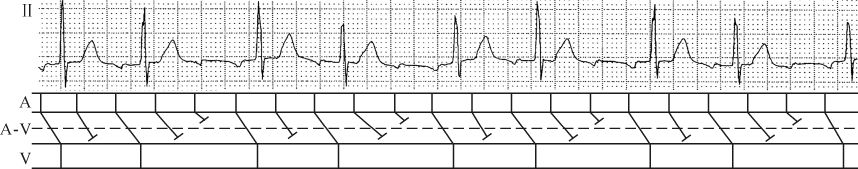
\includegraphics[width=5.80208in,height=1.13542in]{./images/Image00151.jpg}
 \captionsetup{justification=centering}
 \caption{心房扑动伴房室交接区B型交替性文氏周期(上层5:4文氏现象,下层2:1阻滞)}
 \label{fig10-7}
  \end{figure} 

(8)反映房室交接区三层阻滞:选用A、A-V、V三行图,其中A-V行宽达1.2cm,并将其一分为三(图\ref{fig24-9}~图\ref{fig24-12})。

\protect\hypertarget{text00018.html}{}{}

\protect\hypertarget{text00018.htmlux5cux23chapter18}{}{}

\chapter{早 搏}

\protect\hypertarget{text00018.htmlux5cux23subid124}{}{}

\section{概 述}

心脏任何部位产生的搏动,当其出现时间较基本心律(多为窦性心律)提早时,称为过早搏动(简称早搏)。心电图特征为提早出现的P′(P)波或P′(P)-QRS-T波群或QRS-T波群,其后多有较基本周期为长的代偿间歇。

\protect\hypertarget{text00018.htmlux5cux23subid125}{}{}

\subsection{早搏的类型}

有多种分类方法,主要有以下5种:

(1)根据早搏起源的部位:分为窦性、窦房交接性、房性、房室交接性、室性及房室旁道性早搏,其中以房性、室性早搏最为多见。

(2)根据早搏起搏点的多少:分为单源性、双源性、多源性早搏。

(3)根据早搏产生的机制:分为折返型、自律性增高型、并行心律型和触发活动型早搏等。

(4)根据早搏提早的程度:分为收缩早期、中期、晚期及舒张早期、中期、晚期早搏。

(5)根据早搏起源部位与主导节律部位的异同:分为异腔性早搏、同腔性早搏,前者见于窦性心律伴房室交接性早搏或室性早搏,后者见于窦性心律伴窦性早搏、房性心律伴房性早搏、房室交接性心律伴房室交接性早搏或室性早搏、室性心律伴室性早搏等。

\protect\hypertarget{text00018.htmlux5cux23subid126}{}{}

\subsection{早搏发生的机制}

(一)折返学说

1.形成折返的基本条件

(1)必须存在解剖学或电生理学上一个有效的折返环路,即在结构或功能上至少存在两条传导径路。

(2)该折返环路的两条径路不应期不一致,其中一条径路存在单向传导或单向阻滞。

(3)另一条径路内出现充分的传导延缓,以利于产生足够长的折返时间,使原来激动过的传导组织和心肌脱离不应期。

2.折返环路的类型

(1)微折返:该折返环路多发生在浦肯野纤维与心室肌连接处,因浦肯野纤维的“Y”形分叉与心室肌所构成的立体三角形是形成微折返的解剖基础。亦可发生在窦房结、窦房交接区、结间束、心房肌、房室交接区、束支、分支及心室肌等部位。微折返是产生早搏的主要电生理机制。

(2)巨折返:该折返激动所经过的折返环较大,多发生在较大范围的心房、心室内或双束支、希氏束所构成的折返环。

3.折返环路的折返模式

(1)解剖决定性折返:激动围绕正常或异常的解剖结构而形成的环行通道,如房室旁道、束支等。

(2)功能决定性折返:该折返环路由心肌细胞电生理特征的差异性所决定,折返环细小,无固定长度,有5种模式:①主导环折返;②各向异性折返:指心肌组织结构的各向异性和电传导功能的各向异性而引起的折返,右心房下部结构的各向异性最为明显,故右心房下部依赖性房性心律失常发生率高于其他部位;③激动传导的反折:指激动在紧紧相邻的两条心肌纤维中一条前向传导,并经另一条折回,多见于浦肯野纤维、梗死区周围的心肌组织;④螺旋波折返;⑤8字形折返,发生在缺血心肌中,包括了解剖决定性和功能决定性两种折返模式。

4.折返性早搏的心电图类型

由前一心搏的激动沿着折返环路内折返再次引起心房或心室除极而产生提早出现的搏动,称为折返性早搏。激动在折返环路内折返传至心房或心室使其除极所需的时间,称为早搏的偶联间期或联律间期、配对间期。根据激动的折返环路是否易变、传导速度是否一致、折返终点有无改变及是否连续折返等,可有7种心电图表现。

(1)偶联间期固定、P′或R′波形一致:最常见,常呈显性或隐性二、三联律。系折返激动沿着同一折返环路等速传导到达同一终点,前者折返环路内存在着两个水平阻滞区,近端多为固定性2:1阻滞,远端为不固定的隐匿性阻滞;而后者折返环路内存在着三个水平阻滞区,近端多为固定性3:1阻滞,中、远端为不固定的隐匿性阻滞。当折返激动能通过远端时,就出现显性早搏;反之,则形成隐匿性早搏,可从其对侵入同一环路的下一次激动的影响上予以识别。若各显性早搏之间窦性搏动的个数呈2n+1规律(n为自然数),则为隐匿性早搏二联律;若呈3n+2规律,则为隐匿性早搏三联律。

(2)偶联间期固定,而P′或R′波形各异:当折返环路和折返终点发生改变,但传至心房或心室所需的时间相等时,则出现P′或R′波形各异而偶联间期固定,常称为多形性早搏。表明传入径路只有一条,而传出径路有多条,其出口位置各异,但传至心房或心室所需的时间是相等的,类似房室结内倒Y型折返径路。

(3)偶联间期、P′或R′波形均不一致:若折返环路、折返时间及折返终点均不一致,则出现偶联间期、P′或R′波形均不一致,常称为多源性早搏。表明存在传出多径路、多出口、不等速传导。

(4)偶联间期呈短、长两种交替或间歇出现,而P′或R′波形一致:当折返环路内纵向分离为快、慢双径路,其出口相同时,便会出现偶联间期呈短、长两种交替或间歇出现而P′或R′波形一致。经快径路传导得短的偶联间期,循慢径路传导得长的偶联间期;或两条长、短不同的折返径路有1个共同出口,类似房室结内Y型折返径路,也可出现偶联间期短、长两种,形成传入双径路。

(5)折返径路内交替性文氏周期、反向文氏周期:P′或R′波形一致而偶联间期逐渐延长或缩短,直至早搏消失,连续出现2~3次窦性搏动,周而复始,表现为折返径路内交替性文氏周期或反向文氏周期。

(6)偶联间期固定、P′或R′波形一致,连续出现≥3次,且其周期相等,形成短阵性早搏性房性或室性心动过速:当折返激动沿着同一折返环路等速传导到达同一终点并且周而复始地循环着,便可形成早搏性心动过速。

(7)偶联间期固定、P′或R′波形一致,连续出现≥3次,但其周期逐渐缩短或延长直至心动过速终止:当折返激动沿着同一折返径路折返时,其传导速度逐渐加快或减慢直至折返中断,周而复始,形成折返径路内反向文氏现象或文氏现象。

(二)异位起搏点自律性增高

心脏不同部位潜在的异位起搏点,当其自律性突然增高时,在基本心律的激动尚未发放或下传以前,抢先发放激动使心房或心室除极,便形成早搏。单源性异位起搏点自律性增高所致的心电图特征为:①P′或R′波形态一致;②偶联间期不等;③两异位搏动之间无倍数关系;④可有房性或室性融合波出现。

(三)并行心律

心脏内有两个起搏点,其中一个起搏点周围有传入阻滞圈保护,免遭主导节律的影响,按照自己固有的频率发放冲动,这个被保护的起搏点就称为并行节律点。其心电图特征是:①偶联间期不等;②两异位搏动之间相等或有一最大公约数;③常有房性或室性融合波出现。

(四)触发活动

在某些病理情况下,心肌动作电位在3相附近可出现较大的振荡性电位变化。若该电位达到阈电位水平时,便能形成1次早搏。该早搏的形成必须由前一动作电位所触发,故称为触发活动。它包括早期后除极和晚期后除极。前者指发生在动作电位的2相平台期或3相早期的振荡性电位变化,产生Ron-T现象的室性早搏;而后者指发生在3相的振荡性电位变化,产生舒张中、晚期早搏。

\protect\hypertarget{text00018.htmlux5cux23subid127}{}{}

\subsection{早搏时相分期与早搏波形变异的关系(表11-1)}

\begin{table}[htbp]
\centering
\caption{早搏时相分期与早搏波形变异的关系}
\label{tab11-1}
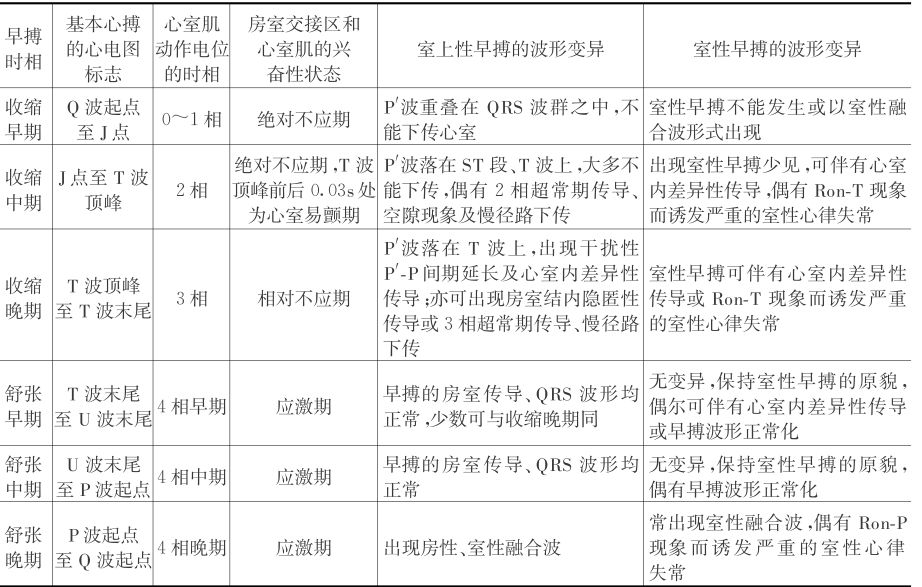
\includegraphics[width=6.22917in,height=3.96875in]{./images/Image00152.jpg}
\end{table}

\protect\hypertarget{text00018.htmlux5cux23subid128}{}{}

\subsection{早搏对窦性节律的影响}

1.早搏后窦性节律顺延

窦性节律被早搏冲动侵入后而引起节律重整,重新积聚兴奋后,按原有的频率发放冲动,但在时间上依次顺延,出现各种代偿间歇。

2.早搏后窦性节律抑制

早搏逆传侵入窦房结后,不仅使其节律重整,还可抑制其起搏点的自律性,使重新积聚兴奋所需的时间较原来的心动周期延长(≥0.32s),可认为有早搏后窦性节律抑制现象。通常早搏出现的时间越早,早搏后窦性节律抑制的程度越明显。

3.早搏后窦性心律不齐

早搏对窦性心律的影响,不仅限于早搏后的第1个窦性搏动,还可影响其后的多个窦性搏动,使P-P间期长短不一,一般先慢后快,存在温醒或起步现象。

4.早搏后窦性节律提前

表现为早搏后第1次被重整搏动的周期缩短,而以后的搏动仍保持原有的周期,与窦性节律重整后其自律性一过性增高有关。

5.早搏后反射性窦性节律抑制

未逆传心房的室性早搏出现超完全代偿间歇,与早搏后反射性窦性节律抑制有关。

\protect\hypertarget{text00018.htmlux5cux23subid129}{}{}

\subsection{早搏的代偿间歇}

早搏的代偿间歇是指早搏的激动至早搏后的第1个基本心搏的时间,似乎是对较短的偶联间期的代偿。习惯上将偶联间期(X)与代偿间歇(Y)之和,即中间夹有早搏的两个基本心搏的时距,与基本心动周期(Z)的2倍进行比较。可将代偿间歇分为以下10种情况:

1.短代偿间歇

其特征为X+Y<Z,即夹有早搏的P-P间期<1个窦性P-P间期。见于窦性回波。

2.无代偿间歇

其特征为X+Y=Z,即夹有早搏的P-P间期等于1个窦性P-P间期。见于各类插入性早搏(间位型早搏),以插入性室性早搏最为常见。

3.次等周期代偿间歇

其特征为X+Y稍>Z,但Y<Z,即夹有早搏的P-P间期略>1个窦性P-P间期,代偿间歇<1个窦性P-P间期。见于窦房交接性早搏、插入性房性早搏伴窦性激动干扰性传出延缓或伴有窦性心律不齐时。

4.等周期代偿间歇

其特征为Y=Z,即代偿间歇等于1个窦性P-P间期。见于同腔性早搏,如窦性心律伴窦性早搏、房性心律伴房性早搏、房室交接性心律伴房室交接性早搏、室性心律伴室性早搏等。

5.不完全性代偿间歇

其特征为X+Y<2Z,Y>Z,即夹有早搏的P-P间期<2个窦性P-P间期,代偿间歇又>1个窦性P-P间期。多见于房性早搏,亦见于房室交接性早搏、室性早搏伴逆传心房且重整窦性节律时,是窦性节律被早搏激动重整的标志。

6.完全性代偿间歇

其特征为X+Y=2Z,即夹有早搏的P-P间期等于2个窦性P-P间期,意指代偿间歇恰好完全代偿了已经缩短的偶联间期,是窦性节律未被早搏激动重整的标志。多见于室性早搏、房室交接性早搏。

7.超完全的代偿间歇

其特征为X+Y>2Z,Y<2Z,即夹有早搏的P-P间期>2个窦性P-P间期,而代偿间歇又<2个窦性P-P间期。见于早搏后窦性节律抑制或反射性窦性节律抑制或伴有显著的窦性心律不齐。

8.特超完全的代偿间歇

其特征为Y>2Z,即代偿间歇>2个窦性P-P间期。见于病窦综合征并发快速性异位心律终止时。

9.延期性代偿间歇

其特征为虽然Y>Z,但最长间歇却发生在早搏后第1个与第2个心搏之间,即插入性室性早搏引起第1个窦性搏动的P-R间期干扰性地显著延长或通过房室结慢径路下传,使第2个窦性搏动落在其绝对不应期内而未能下传心室,出现1个大于窦性P-P间期的较长间歇(图\ref{fig11-1})。多见于窦性心动过缓伴插入性室性早搏。

\begin{figure}[!htbp]
 \centering
 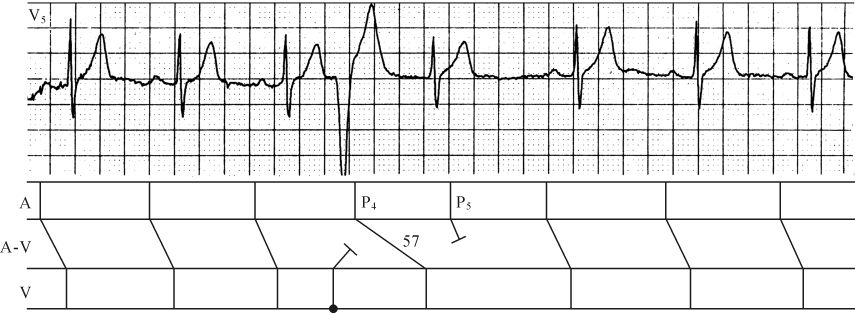
\includegraphics[width=5.78125in,height=2.11458in]{./images/Image00153.jpg}
 \captionsetup{justification=centering}
 \caption{窦性心律不齐、间位型室性早搏伴延期性代偿间歇、房室结内双径路传导或干扰性P-R间期延长或2相超常期传导}
 \label{fig11-1}
  \end{figure} 

10.类代偿间歇

见于心房颤动伴发室性早搏时。心房颤动的R-R间期是绝对不规则的,室性早搏后多可见到一个较长的R-R间歇,因其无基本周期作比较来判断代偿间歇是否完全,故称为类代偿间歇。

\protect\hypertarget{text00018.htmlux5cux23subid130}{}{}

\subsection{早搏的病因及临床意义}

首先要判定早搏是良性的还是病理性的,是器质性的还是功能性的。早搏可发生于正常人中,甚至持续多年不消失,随着年龄的增长,发生的机会也增多。常见病因有以下7种:

1.神经功能性因素

植物神经功能失调、过度劳累、情绪激动、吸烟饮酒、饮浓茶咖啡等均可诱发早搏,颅脑疾患、胆道疾患、鼻部疾患通过脑-心、胆-心、鼻-心神经反射亦可诱发早搏,甲状腺功能亢进、糖尿病时也可通过对植物神经的影响而引起早搏。

2.器质性心脏病

任何感染引起的心肌炎及其后遗症、冠心病、心肌病、高血压性心脏病、风湿性心脏病、先天性心脏病、二尖瓣脱垂、肺源性心脏病、甲亢性心脏病等器质性心脏病均为早搏的常见病因,特别是伴有心力衰竭时,早搏更为常见。

3.各种药物过量或中毒

洋地黄、胺碘酮、普罗帕酮等抗心律失常药物,肾上腺素能药物,如肾上腺素、异丙肾上腺素等,使用过量或中毒时均可发生早搏。

4.电解质紊乱或酸碱平衡失调

低钾血症、高钾血症、低钙血症、低镁血症等电解质紊乱和代谢性酸中毒、碱中毒等均可诱发早搏。

5.低氧血症

各类休克、呼吸衰竭引起的低氧血症,亦会出现早搏。

6.心肌的直接机械性刺激

心脏手术、心导管检查、心脏外伤等均可出现早搏。

7.原发性心电离子通道疾病

先天性长Q-T间期综合征、特发性短Q-T间期综合征、特发性异常J波、Brugada综合征及Lambda波(λ波)等,均可出现早搏甚至出现严重的心律失常而猝死。

\protect\hypertarget{text00018.htmlux5cux23subid131}{}{}

\subsection{早搏心电图分析的步骤}

1.首先确定是否早搏

对于提早出现的搏动,应排除干扰性房室脱节和逸搏心律中的窦性夺获及反复心搏所致的假性早搏。

2.确定早搏的类型、定位诊断及发生机制

根据心电图各导联上P-QRS-T模型,确定早搏起源的基本部位;若是房性、室性早搏,最好能进一步判定它们的大致位置。根据偶联间期固定与否、两异位搏动之间有无倍数关系推测其发生机制。

3.区分早搏出现的时相并分析其传导情况

特别注意收缩中、晚期的早搏因遇及房室交接区、束支的绝对或相对不应期而引起各种传导上的变异,如房性早搏未下传、干扰性P′-R间期延长、心室内差异性传导、2相或3相超常期传导、空隙现象、房室结内慢径路传导等,观察有无早搏本身及其传导变异所引起的同源性心律失常,如房性早搏经慢径路下传诱发房性反复搏动、房性早搏诱发阵发性心房颤动等。

4.对诊断早搏的注意点进行分析

这些注意点包括:早搏数目的分布(是散在、成对出现还是呈二、三联律出现?)、偶联间期的易变性、两异位搏动之间的关系、早搏波形的变异、代偿间歇及早搏与体位、运动、临床症状有无关系等。

5.观察早搏后的心电图改变

这些改变是指早搏激动对基本节律或下一次异位起搏点的影响,如早搏激动有无重整或抑制主导节律、有无早搏后心房内差异性传导、有无出现逸搏及早搏后ST段、T波、U波改变等。

6.了解早搏以外的其他心电图异常

如有无房室肥大、传导阻滞、ST段、T波、U波改变及预激综合征等其他心电图异常改变。

7.结合心电图特征及临床情况,作出完整的心电图诊断,尽可能判断出是良性早搏还是病理性早搏。

\protect\hypertarget{text00018.htmlux5cux23subid132}{}{}

\section{窦性早搏}

1.心电图特征

(1)提早出现的P′波形态与窦性P波一致或略异。

(2)呈等周期代偿间歇。

(3)P′波下传的P′-R间期正常或呈干扰性P′-R间期延长,QRS波形正常或伴心室内差异性传导。

2.鉴别诊断

若窦性搏动呈成对出现,其P-P间期表现为长、短交替而呈窦性二联律时(图\ref{fig11-2}),除窦性早搏二联律外,尚有下列心律失常的可能,需注意鉴别。

\begin{figure}[!htbp]
 \centering
 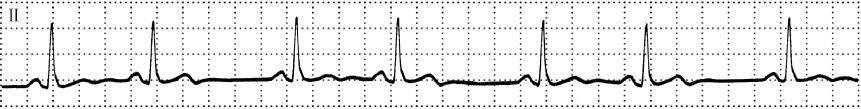
\includegraphics[width=5.82292in,height=0.72917in]{./images/Image00154.jpg}
 \captionsetup{justification=centering}
 \caption{窦性二联律(P波形态一致,P-P间期呈0.76、1.10s交替出现),窦性早搏二联律、3:2文氏型窦房传导阻滞或窦房交接区快、慢径路交替传导有待确诊}
 \label{fig11-2}
  \end{figure} 

(1)3:2文氏型窦房传导阻滞:3:2文氏型窦房传导阻滞时,长P-P间期小于窦性基本P-P间期的2倍,此时与窦性早搏二联律无法区别,除非二联律消失恢复窦性心律时。按照Schamroth的意见,如果二联律消失时所显现的窦性心律,其P-P间期与二联律时较长的P-P间期相等,则此二联律为窦性早搏二联律;若其P-P间期小于二联律时较短的P-P间期,则为3:2文氏型窦房传导阻滞。

(2)3:2二度Ⅱ型窦房传导阻滞:若长P-P间期为短P-P间期的2倍,则此二联律为3:2二度Ⅱ型窦房传导阻滞。

(3)窦房交接区快、慢径路交替传导:二联律时长、短P-P间期之和为二联律消失时所显现的窦性心律基本P-P间期的2倍。经快径路传导时,出现短P-P间期;由慢径路传导时,出现长P-P间期。

(4)房性早搏二联律:提早出现的P′波形态与窦性P波不一致,其后代偿间歇P′-P间期稍长于1个窦性P-P间期而呈不完全性代偿间歇。但当房性早搏的起搏点位于窦房结的附近时,其P′波形态可与窦性P波极为相似,但其后代偿间歇仍稍长于1个窦性P-P间期。

(5)窦性心律不齐:P波形态一致或略异,P-P间期虽然长、短交替出现,但各自P-P间期长短不一,不能用上述心律失常进行解释;若与呼吸周期有关,则屏气后,其P-P间期转为规则。

(6)交替性窦性停搏:有时与窦性心律显著不齐较难鉴别。一般说来,窦性停搏的P-P间期较长,>1.80~2.0s(夜间2.0s)或大于基本周期的1.5倍。

\protect\hypertarget{text00018.htmlux5cux23subid133}{}{}

\section{窦房交接性早搏}

1.心电图特征

(1)提早出现的P′波形态与窦性P波一致或略异。

(2)可呈次等周期、等周期代偿或不完全性代偿间歇。

(3)P′波下传的P′-R间期正常或伴干扰性P′-R间期延长,QRS波形正常或伴心室内差异性传导。

(4)偶联间期多固定(图\ref{fig11-3})。

\begin{figure}[!htbp]
 \centering
 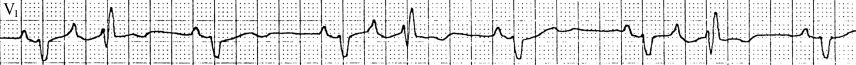
\includegraphics[width=5.78125in,height=0.4375in]{./images/Image00155.jpg}
 \captionsetup{justification=centering}
 \caption{窦性心动过缓、窦房交接区折返性早搏伴房室干扰现象、呈三联律(窦性P-P间期1.20s,P′-P间期1.14~1.20s)}
 \label{fig11-3}
  \end{figure} 

2.鉴别诊断

若窦房交接性早搏呈二联律时,P-P′、P′-P间期表现为短、长交替出现而呈窦性(房性)二联律,需与窦性早搏二联律、房性早搏二联律、3:2窦房传导阻滞、窦房交接区双径路交替传导、交替性窦性停搏等相鉴别。

\protect\hypertarget{text00018.htmlux5cux23subid134}{}{}

\section{房性早搏}

\protect\hypertarget{text00018.htmlux5cux23subid135}{}{}

\subsection{房性早搏的心电图特征}

(1)提早出现的P′波形态与窦性P波不一致。

(2)多呈不完全性代偿间歇,舒张晚期的房性早搏可出现完全性代偿间歇。

(3)可出现各种房室干扰现象:呈阻滞型、房室结内隐匿性传导、干扰性P′-R间期延长及心室内差异性传导,其中前两者称为房性早搏未下传。

(4)若P′波形态不一致而偶联间期相等,则为双形性或多形性房性早搏;若P′波形态及偶联间期均不相同,则为双源性或多源性房性早搏(图\ref{fig11-4}、图\ref{fig11-5})。

\begin{figure}[!htbp]
 \centering
 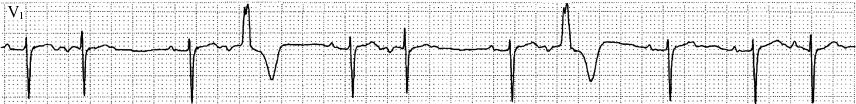
\includegraphics[width=5.78125in,height=0.69792in]{./images/Image00156.jpg}
 \captionsetup{justification=centering}
 \caption{双形性房性早搏,有时伴心室内差异性传导及二联律}
 \label{fig11-4}
  \end{figure} 

\begin{figure}[!htbp]
 \centering
 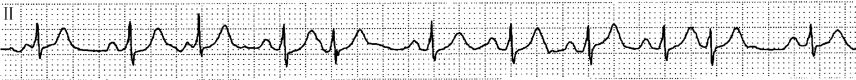
\includegraphics[width=5.78125in,height=0.53125in]{./images/Image00157.jpg}
 \captionsetup{justification=centering}
 \caption{双源性房性早搏}
 \label{fig11-5}
  \end{figure} 

\protect\hypertarget{text00018.htmlux5cux23subid136}{}{}

\subsection{房性早搏的定位诊断}

(1)右心房上部早搏:P′波方向与窦性P波方向一致,即在Ⅰ、Ⅱ、Ⅲ、aVF、V\textsubscript{4}~V\textsubscript{6} 导联P′波直立,aVR导联P′波倒置。

(2)右心房下部早搏:其心房除极向量指向左上方,在Ⅰ、aVL、V\textsubscript{4}~V\textsubscript{6} 导联P′波直立,而Ⅱ、Ⅲ、aVF导联P′波倒置。

(3)左心房上部早搏:Ⅰ、aVL、V\textsubscript{4} ~V\textsubscript{6}导联P′波倒置,Ⅱ、Ⅲ、aVF导联P′波直立。若V\textsubscript{1}导联P′波呈圆顶标枪型,则起源于左心房后壁;若V\textsubscript{1}导联P′波倒置,则起源于左心房前壁。

(4)左心房下部早搏:P′波为逆行P\textsuperscript{-}波,在Ⅰ、aVL、V\textsubscript{4} ~V\textsubscript{6}、Ⅱ、Ⅲ、aVF导联P′波倒置,aVR导联P′波直立,再根据V\textsubscript{1}导联P′波形态区别起源于左心房前壁或后壁。

\protect\hypertarget{text00018.htmlux5cux23subid137}{}{}

\subsection{房性早搏对窦性节律的影响}

(一)窦房结对不同偶联间期的房性早搏可有4种不同的反应区域

(1)窦房结周围干扰区(Ⅰ区):偶联间期较长的房性早搏,其冲动逆传时与窦性激动在窦房交接区发生绝对干扰,出现完全性代偿间歇。多见于舒张中、晚期的房性早搏。

(2)窦房结内干扰区(Ⅱ区):偶联间期较短的房性早搏,其冲动逆传侵入窦房结使其节律重整,出现不完全性代偿间歇。多见于收缩晚期、舒张早期的房性早搏。

(3)窦房结不应区(Ⅲ区):偶联间期短的房性早搏,其冲动逆传时遇及窦房结的不应期而未能侵入,出现无代偿间歇而呈间位型房性早搏,但有时窦性激动在传出过程中遇及其相对不应期,而使窦性P波后延,出现间位型房性早搏前后的窦性P-P间期较基本窦性P-P间期略长。多见于收缩中期的房性早搏(图\ref{fig11-6})。

\begin{figure}[!htbp]
 \centering
 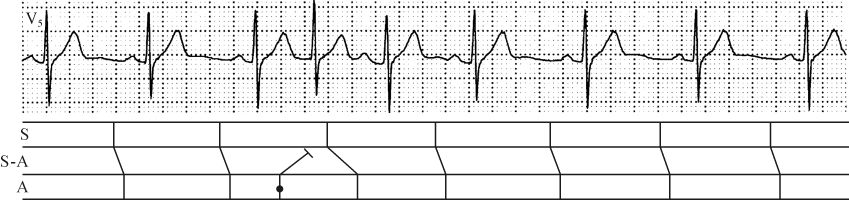
\includegraphics[width=5.73958in,height=1.34375in]{./images/Image00158.jpg}
 \captionsetup{justification=centering}
 \caption{间位型房性早搏引起S-A间期延长致窦性P波后延}
 \label{fig11-6}
  \end{figure} 

(4)窦房折返区(Ⅳ区):偶联间期更短的房性早搏,其冲动沿着窦房交接区慢径路逆传侵入窦房结,同时又循快径路折回心房,形成窦性回波或(和)窦房折返性心动过速。Ⅲ区的房性早搏遇及窦房结的不应期,而Ⅳ区的房性早搏却能引起窦房折返,似乎存在矛盾现象,可用窦房交接区空隙现象或双径路传导学说来解释:①空隙现象:当窦房结不应期大于心房不应期时,Ⅲ区内的房性早搏逆传时遇及窦房结的不应期而受阻,而Ⅳ区内的房性早搏逆传时却遇及心房、窦房交接区的相对不应期而缓慢逆传到窦房结,此时的窦房结已脱离了不应期被房性早搏重整,且同时引发窦房交接区折返;②双径路传导:窦房结周围分离为快、慢两条传导径路,Ⅲ区内的房性早搏沿快径路逆传遇及窦房结的不应期而受阻,而Ⅳ区内的房性早搏沿慢径路逆传到窦房结,此时的窦房结已脱离了不应期被房性早搏重整,且同时又循快径路折回心房形成窦性回波或(和)窦房折返性心动过速(图\ref{fig1-18})。

(二)少数房性早搏可抑制或促发窦性激动的发放

(1)房性早搏引起窦房结功能抑制:房性早搏重整窦性节律后,窦性起搏点需要较长时间方能恢复其原有的自律性,出现超完全代偿间歇或特超完全代偿间歇。多见于窦房结功能低下者。

(2)房性早搏促进窦性节律提前发放:表现为早搏后第1次被重整搏动的周期缩短,而以后的搏动仍保持原有的周期,与窦性节律重整后其自律性一过性增高有关(图\ref{fig11-7})。

\begin{figure}[!htbp]
 \centering
 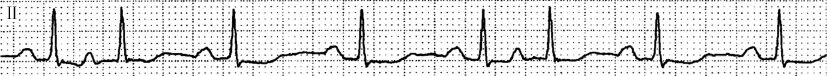
\includegraphics[width=5.58333in,height=0.51042in]{./images/Image00159.jpg}
 \captionsetup{justification=centering}
 \caption{房性早搏促进窦性节律提前发放(P′-P间期<P-P间期)、轻度ST-T改变}
 \label{fig11-7}
  \end{figure} 

(三)根据房性早搏的代偿间歇,测算窦房传导时间及窦房结功能变动时间

从梯形图中可知,在正常情况下,房性早搏代偿间歇(Y)的长度=1个窦性P-P间期(Z)+房窦传导时间(P′-S时间)+窦房传导时间(S-P时间),P′-S时间与S-P时间大致相等,故S-P时间=(Y-Z)/2,正常值为0.07~0.16s,测量房性早搏的代偿间歇可大致地反映窦房传导时间及窦房结起搏点的功能。有学者主张采用窦房结功能变动时间来评估窦房结的起搏功能和窦房传导功能。窦房结功能变动时间=Y-Z,即代偿间歇-窦性基本P-P间期,正常值为0.14~0.32s。如果正常,可认为窦房结的起搏功能及窦房传导功能大致正常;如>0.32s,则窦房结的起搏功能或窦房传导功能有减退,其值愈大,诊断可靠性也愈大(图\ref{fig11-8})。

\begin{figure}[!htbp]
 \centering
 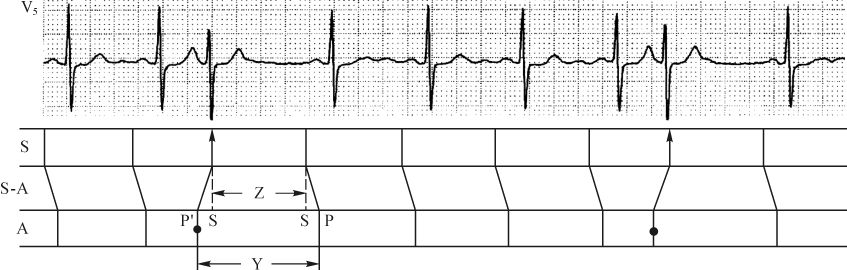
\includegraphics[width=5.71875in,height=1.82292in]{./images/Image00160.jpg}
 \captionsetup{justification=centering}
 \caption{窦房结功能变动时间的测算(P′-P间期-P-P间期,即Y-Z)}
 \label{fig11-8}
  \end{figure} 

\protect\hypertarget{text00018.htmlux5cux23subid138}{}{}

\subsection{房性早搏的房室传导情况}

发生在不同时相的房性早搏,因遇及房室交接区、束支或心室肌的绝对不应期、相对不应期、应激期而出现各种房室干扰现象、意外性传导或正常传导等。

1.房性早搏未下传

房性早搏未下传包括阻滞型房性早搏和房性早搏伴房室交接区内隐匿性传导。前者因遇及房室交接区的绝对不应期而未能下传,后者因遇及房室交接区的绝对不应期向相对不应期的过渡阶段,该激动虽然未能下传心室,但在房室交接区下传了一定的深度,对下一次激动的传导和该部位激动的形成带来影响,故称为隐匿性传导。见于收缩中、晚期的房性早搏。

2.房性早搏伴干扰性P′-R间期延长

房性早搏遇及房室交接区的相对不应期而发生干扰性P′-R间期延长,其P′-R间期的长短与R-P′间期呈反比关系,即R-P′间期短,其P′-R间期长,R-P′间期长,其P′-R间期短。见于收缩晚期的房性早搏,少数见于舒张早期的房性早搏。

3.房性早搏伴心室内差异性传导

房性早搏下传心室时,若遇及左、右束支及其分支之间的传导时间互差>25ms,便会出现心室内差异性传导。QRS波群表现为右束支或左束支阻滞图形或伴左前分支或左后分支阻滞图形,偶尔心室内差异性传导发生在浦肯野纤维或心室肌内,表现为不定型心室内传导阻滞图形。见于收缩晚期、舒张早期的房性早搏。

4.房性早搏伴束支间的蝉联现象

房性早搏二联律时,其下传QRS波群呈交替性左、右束支阻滞图形,这一特殊的心室内差异性传导可用束支间的蝉联现象来解释。在生理情况下,右束支不应期比左束支长,当房性早搏下传时,由于右束支尚处于前一次窦性搏动下传所产生的不应期中,激动循已脱离不应期的左束支下传,使左心室先除极,激动穿过室间隔进入右心室并逆传至右束支,使早搏的QRS波群呈右束支阻滞图形。由于右束支除极较晚,距离下一个窦性搏动下传的右束支周期变短,其后的不应期也随之缩短,而左心室比右心室早除极,距离下一个窦性激动下传的左束支周期比右束支周期相对延长,其后的不应期也较右束支延长,故第2个房性早搏下传时适逢左束支不应期,于是激动循右束支下传,QRS波群呈左束支阻滞图形。由于循右束支下传的激动又可隐匿性逆传到左束支,使左束支较晚除极,故左束支周期缩短,其后的不应期也相应缩短,这样,下一个房性早搏下传时,右束支仍处于不应期,激动循已脱离不应期的左束支下传,QRS波群又呈右束支阻滞图形。如此两侧束支内交替隐匿性传导,便不断发生左、右束支交替性阻滞图形,直至房性早搏二联律的形式结束而告终(图\ref{fig11-9})。

\begin{figure}[!htbp]
 \centering
 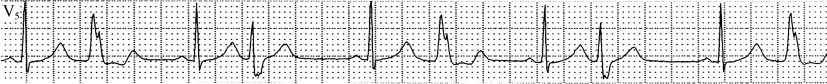
\includegraphics[width=5.58333in,height=0.5625in]{./images/Image00161.jpg}
 \captionsetup{justification=centering}
 \caption{房性早搏二联律伴交替性左、右束支阻滞型心室内差异性传导(束支间的蝉联现象)}
 \label{fig11-9}
  \end{figure} 

5.房性早搏伴正常房室传导

房性早搏下传的P′-R间期、QRS波形均正常。见于舒张期的房性早搏。

6.房性早搏伴旁道下传

(1)房性早搏通过James束下传:当房性早搏通过James束下传心室时,其P′-R间期缩短(<0.12s),QRS波形正常或伴心室内差异性传导。

(2)房性早搏通过房室旁道下传:当房性早搏通过Kent束下传心室时,其P′-R间期缩短(<0.12s),有“δ”波,QRS波群宽大畸形,符合预激波形的特征(图\ref{fig11-10})。

\begin{figure}[!htbp]
 \centering
 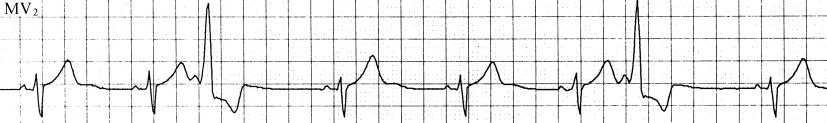
\includegraphics[width=5.58333in,height=0.82292in]{./images/Image00162.jpg}
 \captionsetup{justification=centering}
 \caption{房性早搏通过Jams束下传伴心室内差异性传导或Kent束下传心室}
 \label{fig11-10}
  \end{figure} 

7.房性早搏伴房室传导阻滞

发生在舒张中、晚期的房性早搏仍未能下传心室时,应考虑3相性(快频率依赖性)二度房室传导阻滞;若下传的P′-R间期较窦性P-R间期显著地延长,则应考虑3相性一度房室传导阻滞或房室结内慢径路传导。

8.房性早搏伴房室意外性传导

发生在收缩中期(J点至T波顶峰)的房性早搏,理应不能下传心室,但有时可意外地下传,称为房性早搏伴房室意外性传导,与房室交接区2相超常期传导、慢径路传导或空隙现象等有关。

\protect\hypertarget{text00018.htmlux5cux23subid139}{}{}

\subsection{房性早搏揭示房室结内双径路、三径路传导}

1.房性早搏揭示房室结内顺向型双径路传导

(1)出现在收缩期的房性早搏,即P′波落在J点、ST段、T波上,其下传的P′-R间期固定地延长,偶尔略有长短(<0.06s),且R-P′间期与P′-R间期不呈反比关系的矛盾现象,不能以干扰性P′-R间期延长来解释(图\ref{fig11-11})。

\begin{figure}[!htbp]
 \centering
 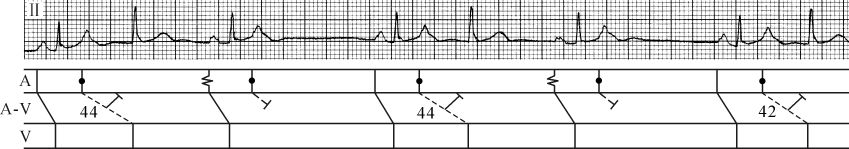
\includegraphics[width=5.73958in,height=1in]{./images/Image00163.jpg}
 \captionsetup{justification=centering}
 \caption{房性早搏二联律伴P′-R间期延长(提示房室结慢径路下传)、阻滞型及早搏后心房内差异性传导}
 \label{fig11-11}
  \end{figure} 

(2)房性早搏诱发房性反复搏动,即出现P′-QRS-P\textsuperscript{-}-QRS或P′-QRS-P\textsuperscript{-} 、P′-P\textsuperscript{-}序列的心房回波,其R-P\textsuperscript{-} 间期<0.08s。

(3)房性早搏诱发慢-快型房室结内折返性心动过速,其P\textsuperscript{-}波落在J点附近,R-P\textsuperscript{-}间期<0.08s,且R-P\textsuperscript{-} 间期<P\textsuperscript{-}-R间期。

2.房性早搏揭示房室结内顺向型三径路传导

(1)房性早搏P′波或窦性P波落在ST段、T波上,其下传的P′-R间期、P-R间期出现长、短两种,且互差≥0.06s,R-P′间期与P′-R间期不呈反比关系的矛盾现象(图\ref{fig50-10})。

(2)同一房性早搏后连续出现两种形态的逆行P\textsuperscript{-}波,呈$\text{P}^\prime-\text{QRS}-\text{P}_1^--\text{P}_2^-$
序列,$\text{R}-\text{P}_1^-$
间期和$\text{R}-\text{P}_2^-$
间期各自固定,且互差≥0.06s,即各有固定的$\text{P}^\prime-\text{P}_1^-$
间期与$\text{P}^\prime-\text{P}_2^-$
间期,且能重复出现(图\ref{fig11-12})。

\begin{figure}[!htbp]
 \centering
 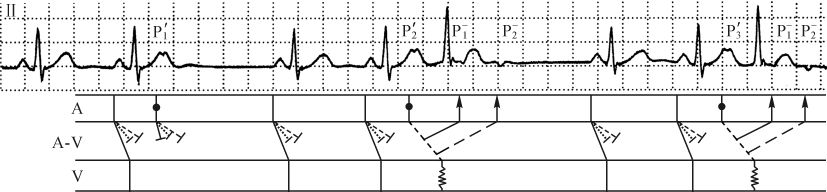
\includegraphics[width=5.58333in,height=1.29167in]{./images/Image00169.jpg}
 \captionsetup{justification=centering}
 \caption{房性早搏三联律、呈阻滞型或心室内差异性传导、房性反复搏动揭示房室结内顺向型三径路传导}
 \label{fig11-12}
  \end{figure} 

(3)同一房性早搏后连续出现两种形态的逆行P\textsuperscript{-}波,呈$\text{P}^\prime-\text{P}_1^--\text{P}_2^-$
序列,各有固定的$\text{P}^\prime-\text{P}_1^-$
间期、$\text{P}^\prime-\text{P}_2^-$
间期,且能重复出现。第2、3两种情况易误诊为起源于心房下部的阻滞型房性早搏。

\protect\hypertarget{text00018.htmlux5cux23subid140}{}{}

\subsection{房性早搏揭示窦性并行心律}

偶联间期不等的房性早搏或多源性房性早搏,出现完全性代偿间歇,其激动均不能逆传侵入窦房结使其节律重整,窦性激动按原有的节律发放激动,插入性房性早搏可使窦性P波后延(图\ref{fig16-2}、图\ref{fig16-3})。

\protect\hypertarget{text00018.htmlux5cux23subid141}{}{}

\subsection{房性早搏诱发其他心律失常}

1.房性早搏诱发窦性回波

窦房结及其周围组织的电生理功能和房室结有一定的相似性,细胞间的不应期和传导性均存在明显差异,窦房结及窦房交接区可分离为两条传导功能不同的径路。适时的房性早搏激动由一条径路逆传侵入窦房结,再经另一条径路传出,再次激动心房,形成窦性回波。在房性早搏后出现P′-P-P序列,其中第1个P波为窦性回波,第2个P波为房性早搏重整窦性节律后窦性所发放的第1个激动,上述P′-P-P序列中的P-P间期<1个窦性P-P间期(图\ref{fig1-19})。需注意与间位型房性早搏相鉴别。

2.房性早搏诱发窦房折返性心动过速

适时的房性早搏激动逆传侵入窦房结或窦房交接区并出现连续折返现象,形成窦房结内或窦房交接区折返性心动过速。具有突然发生和突然终止的特点,绝大多数呈短阵性发作,且每次发作心搏数<10~20次,可反复发作,频率为100~150次/min,其P波形态与窦性P波一致或略异;同一次发作的频率往往是一致的,但各次发作时的频率又是多变的;心动过速终止后的代偿间歇,可呈不完全性代偿间歇或等周期代偿间歇。

3.房性早搏诱发快速性房性心律失常

较多见,偶联间期为0.20~0.30s的房性早搏,易落在心房易颤期内而诱发房性心动过速、心房颤动或心房扑动等快速性房性心律失常。Killip及Gault提出计算偶联指数公式:偶联指数等于偶联间期/房性早搏前的1个窦性P-P间期。当偶联指数<0.50时,心房颤动发生率增高;当偶联指数>0.60时,心房颤动发生率减少(图\ref{fig11-13})。

\begin{figure}[!htbp]
 \centering
 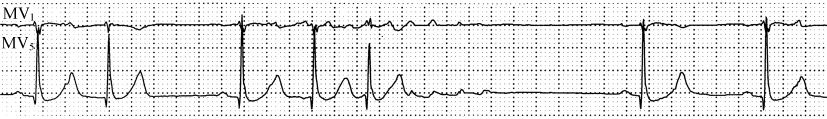
\includegraphics[width=5.58333in,height=0.80208in]{./images/Image00173.jpg}
 \captionsetup{justification=centering}
 \caption{房性早搏诱发短阵性心房扑动伴房室结内隐匿性传导}
 \label{fig11-13}
  \end{figure} 

4.房性早搏诱发房性反复搏动及反复性心动过速

适时房性早搏通过房室结内慢径路下传心室,同时又循快径路逆传到心房,形成房性反复搏动或慢-快型房室结内折返性心动过速,形成P′-QRS-P\textsuperscript{-}-QRS-P\textsuperscript{-} -QRS序列,其R-P\textsuperscript{-}间期<P\textsuperscript{-} -R间期,且R-P\textsuperscript{-}间期<0.08s。

5.房性早搏诱发房室折返性心动过速

适时的房性早搏可诱发顺向型、逆向型房室折返性心动过速。以前者多见,约占95\%。

(1)顺向型房室折返性心动过速:其折返环路为心房→房室正道前传→心室→房室旁道逆传→心房,周而复始。心电图特征为:①房性或室性早搏可诱发或终止心动过速;②心室率很快,绝大多数≥200次/min,R-R间期规则或长、短交替;③QRS波形正常和(或)呈功能性束支阻滞图形,两者波形并存时,若后者的R-R间期较前者延长≥35ms,且同时伴R-P\textsuperscript{-}间期延长,说明旁道在束支阻滞的同侧;④常伴有QRS波幅电交替,窄QRS波心动过速伴QRS波幅电交替对判断顺向性房室折返性心动过速具有高度的特异性;⑤在ST段或T波上必有逆行P\textsuperscript{-}波,其R-P\textsuperscript{-} 间期<P\textsuperscript{-}-R间期,且R-P\textsuperscript{-}间期>0.08s,可与房室结内折返性心动过速相鉴别。

(2)逆向型房室折返性心动过速:约占5\%,其折返环路为心房→房室旁道前传→心室→房室正道逆传→心房,周而复始。形成这种折返需具备3个条件:①旁道前传的有效不应期比房室结短,而逆传的有效不应期比房室结长;②房室正道有稳定的逆传能力;③有足够长的折返时间。心电图特征为:①房性或室性早搏可诱发或终止心动过速;②心室率很快,通常≥200次/min,R-R间期规则;③QRS波群宽大畸形,呈完全性预激波形,与既往窦性心律时预激波形相似;④如能辨认出逆行P\textsuperscript{-}波,则R-P\textsuperscript{-} 间期>P\textsuperscript{-}-R间期,且P\textsuperscript{-}-R间期<0.12s。与室性心动过速鉴别有时很困难,最有用的鉴别要点是:该宽大畸形QRS波群是否与既往预激波形或室性早搏波形相似,有无逆行P\textsuperscript{-}波及房室分离。

6.房性早搏诱发窦性停搏

在窦房结功能低下时,房性早搏尤其是短阵性房性心动过速可抑制窦性激动的发放,引发窦性停搏。

7.房性早搏诱发阵发性二度、三度房室传导阻滞

适时的房性早搏可诱发阵发性二度、三度房室传导阻滞(图\ref{fig11-14})。与房性早搏在房室交接区内发生隐匿性传导,导致其后的窦性激动亦在房室交接区内发生连续的隐匿性传导或房室交接区同时存在3相、4相阻滞有关。

\begin{figure}[!htbp]
 \centering
 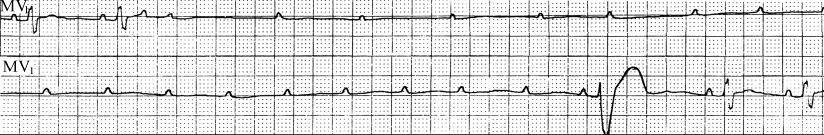
\includegraphics[width=5.5625in,height=0.90625in]{./images/Image00174.jpg}
 \captionsetup{justification=centering}
 \caption{MV\textsubscript{1}导联连续记录,显示成对阻滞型房性早搏诱发阵发性三度房室传导阻滞伴心室停搏、室性逸搏诱发房室交接区韦金斯基现象}
 \label{fig11-14}
  \end{figure} 


8.房性早搏诱发继发性室性早搏二联律

房性早搏产生的较长代偿间歇,易诱发继发性室性早搏,室性早搏后的长间歇又为下一个继发性室性早搏创造了条件,周而复始,便形成偶联间期固定的单源性室性早搏二联律。

9.房性早搏诱发非时相性心房内差异性传导

(1)心电图特征:①早搏代偿间歇之后,出现1个或连续数个窦性P波形态发生改变;②变形的P波又是窦性P波应出现的位置,且多次重复出现(图\ref{fig11-15})。

\begin{figure}[!htbp]
 \centering
 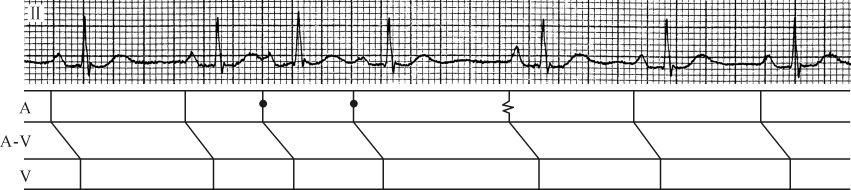
\includegraphics[width=5.75in,height=1.28125in]{./images/Image00175.jpg}
 \captionsetup{justification=centering}
 \caption{成对房性早搏诱发非时相性心房内差异性传导或房性逸搏}
 \label{fig11-15}
  \end{figure} 

(2)发生机制:①早搏在心房传导束内发生隐匿性传导:由于结间束、房间束的不应期不一致,房性早搏在逆传窦房结时,可在窦房交接区内产生隐匿性折返,并隐匿性地激动了结间束、房间束,使其产生新的不应期,影响下一个窦性激动的正常除极致P波形态改变;②心房内4相性阻滞:房性早搏产生较长的代偿间歇,结间束或房间束发生4相性阻滞。

(3)鉴别诊断:应注意与窦房结内游走节律、窦房结至心房内游走节律、房性逸搏及房性融合波相鉴别。

10.房性早搏诱发窦房结内游走节律

房性早搏逆传重整窦性节律后,可引起窦房结起搏点暂时转移或游走,出现早搏后的P-P间期不规则,P波形态由低→高或由高→低周期性改变,直至P-P间期规则,P波形态一致。据此特征可与非时相性心房内差异性传导相鉴别。

11.房性早搏诱发房性逸搏或房性逸搏心律

房性早搏逆传可抑制窦性激动的发放,心房起搏点被动性地发放激动,形成房性逸搏或逸搏心律。其延迟出现的P′波形态与窦性P波不一致,逸搏周期多固定,且较窦性周期长,在1.0~1.20s。

12.房性早搏诱发加速的房性逸搏或加速的房性逸搏心律

房性早搏代偿间歇后稍延迟出现的P′波形态与窦性P波不一致,逸搏周期多固定且较窦性周期短,其周期<1.0s,频率>60次/min。

13.房性早搏诱发房室交接性或室性逸搏及其逸搏心律

房性早搏引起的较长代偿间歇,可诱发房室交接性、室性逸搏或逸搏心律。

\protect\hypertarget{text00018.htmlux5cux23subid142}{}{}

\subsection{房性早搏的鉴别诊断}

1.未下传的房性早搏二联律

若P′波落在T波上而未能下传时,则极易误诊为窦性心动过缓,需特别注意T波形态的改变。

2.未下传的房性早搏三联律

若P′波落在T波上,不能识别或未注意识别时,则表现为短的窦性周期与长的窦性周期(实为夹有1个未下传房性早搏的偶联间期和代偿间歇之和)相交替的窦性二联律,类似于窦性早搏二联律、交替性窦性停搏、3:2窦房传导阻滞、显著窦性心律不齐、窦房交接区快慢径路交替性传导等。鉴别时需注意寻找P′波及T波形态改变,必要时加做S\textsubscript{5}导联、食道导联或放大电压、加快走纸速度使P′波显露。

3.心房下部早搏与房室交接性早搏的鉴别

心房下部早搏与逆行P\textsuperscript{-}波位于QRS波群之前的房室交接性早搏均表现为逆行P\textsuperscript{-}波。两者区别主要根据P\textsuperscript{-}-R间期的长短,若P\textsuperscript{-}-R间期≥0.12s,则为前者;若P\textsuperscript{-}-R间期<0.12s,则为后者。

4.房性早搏伴心室内差异性传导与室性早搏的鉴别

两者鉴别主要根据宽大畸形QRS-T波群,其前有无相关的P′波及代偿间歇是否完全。

5.房性早搏与窦性夺获的鉴别

窦性夺获多见于干扰性房室脱节时,虽然亦是提早出现,但它的发生部位是窦性P波的位置,仔细测量两者不难鉴别。

\protect\hypertarget{text00018.htmlux5cux23subid143}{}{}

\section{房室交接性早搏}

\protect\hypertarget{text00018.htmlux5cux23subid144}{}{}

\subsection{房室交接区结构、传导的基本特征}

房室交接区包括房-结区、结区和结-希区3个区,其中结区在解剖和电生理上具有迷路样结构、纵向分离为双径路或多径路、横向分离为双层阻滞或多层阻滞及递减性传导等特征,其激动大多具有双向传导,前向传导产生QRS波群,逆向传导产生P\textsuperscript{-}波。

\protect\hypertarget{text00018.htmlux5cux23subid145}{}{}

\subsection{房室交接性早搏的心电图特征}

(1)提早出现QRS-T波群呈室上性:即提早出现QRS-T波群与窦性一致或稍有差异,若伴有心室内差异性传导、束支阻滞,则与室性早搏较难鉴别。

(2)P\textsuperscript{-} 波与QRS波群的关系:P\textsuperscript{-}波与QRS波群的关系反映了早搏起搏点的位置及前向传导与逆向传导的时间差。P\textsuperscript{-}波可位于QRS波群之前,其P\textsuperscript{-}-R间期<0.12s;亦可位于QRS波群之中或位于QRS波群之后,其R-P\textsuperscript{-}间期<0.16s;多数因逆传受阻或发生在舒张晚期,其QRS波群前、中、后始终无P\textsuperscript{-}波,而可有窦性P波存在。P\textsuperscript{-}-R间期或R-P\textsuperscript{-}间期并不代表房室或室房传导时间,而是前向传导与逆向传导的时间差。

(3)代偿间歇大多呈完全性代偿间歇,少数可呈不完全性代偿间歇,这取决于P\textsuperscript{-}波有无逆传侵入窦房结使其节律重整。

\protect\hypertarget{text00018.htmlux5cux23subid146}{}{}

\subsection{房室交接性早搏前向传导情况与鉴别诊断}

1.房室交接性早搏伴非时相性心室内差异性传导

提早出现QRS-T波群的形态与窦性略异,时间正常,仅QRS波幅略有高低或起始向量不一致,这与起搏点起源部位及下传途径有关,如起源于房室交接区边缘部分、结-希区及激动部分通过Mahaim纤维下传心室(图\ref{fig11-16})。若QRS波形差异较大和(或)时间略增宽(≤0.11s),尤其是未见相关的P\textsuperscript{-}波,则诊断高位室性早搏较为妥当。

\begin{figure}[!htbp]
 \centering
 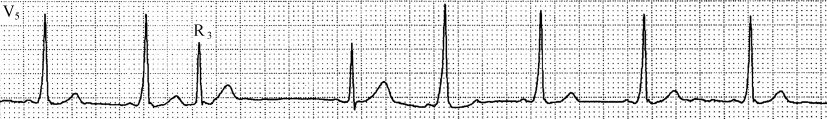
\includegraphics[width=5.58333in,height=0.80208in]{./images/Image00176.jpg}
 \captionsetup{justification=centering}
 \caption{房室交接性早搏伴非时相性心室内差异性传导(R\textsubscript{3})并揭示Kent束4相性阻滞}
 \label{fig11-16}
  \end{figure} 


2.房室交接性早搏伴心室内差异性传导

只有P\textsuperscript{-} 波位于QRS波群之前且P\textsuperscript{-}-R间期<0.12s或P\textsuperscript{-}波位于QRS波群之后且R-P\textsuperscript{-}间期<0.16s,则宽大畸形QRS波群方能诊断为房室交接性早搏伴心室内差异性传导(图\ref{fig11-17})。若P\textsuperscript{-}波重叠于QRS波群之中不能识别或无P\textsuperscript{-}波,则该宽大畸形QRS波群宜诊断为室性早搏。

\begin{figure}[!htbp]
 \centering
 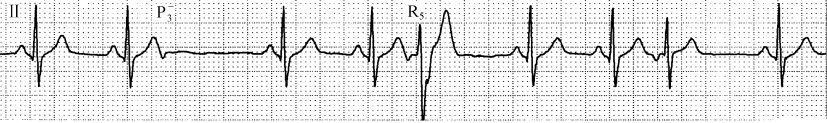
\includegraphics[width=5.58333in,height=0.82292in]{./images/Image00177.jpg}
 \captionsetup{justification=centering}
 \caption{房室交接性早搏时伴房室前向性阻滞(P\textsuperscript{-}3)及心室内差异性传导(R\textsubscript{5} )}
 \label{fig11-17}
  \end{figure} 


3.房室交接性早搏伴干扰性P\textsuperscript{-} -R间期延长(≥0.12s)

提早出现的P\textsuperscript{-}波多发生在收缩晚期或舒张早期,前向传导遇及房室交接区组织的相对不应期而出现传导延缓,产生干扰性P\textsuperscript{-}-R间期延长,此时与心房下部早搏难以区别。但若同一份心电图上见到P\textsuperscript{-}-R间期<0.12s的室上性早搏,则有利于房室交接性早搏的诊断。

4.房室交接性早搏伴干扰性房室前向传导中断

提早出现的P\textsuperscript{-}波多发生在收缩中、晚期,其后未见QRS-T波群跟随。系该早搏前传遇及房室交接区组织的绝对不应期而未能下传,但能逆传心房产生P\textsuperscript{-}波,此时与阻滞型心房下部早搏难以鉴别;但若同一份心电图上有下传的心房下部早搏或下传的房室交接性早搏,则有利于两者的区别(图\ref{fig11-17})。

5.房室交接性早搏伴3相性一度、二度房室传导阻滞

若提早出现的P\textsuperscript{-}波发生在舒张中、晚期而出现P\textsuperscript{-}-R间期延长(≥0.12s)或无QRS-T波群跟随者,则应考虑3相性一度、二度房室传导阻滞。

\protect\hypertarget{text00018.htmlux5cux23subid147}{}{}

\subsection{房室交接性早搏逆向传导情况}

1.房室交接性早搏伴阻滞性逆传受阻

最常见,不论房室交接性早搏的时相如何,提早出现的室上性QRS波群前后始终没有P\textsuperscript{-}波。这可能与房室结迷路样结构和递减性传导有关。

2.房室交接性早搏伴干扰性逆传受阻

舒张中、晚期房室交接性早搏逆传通过房室交接区时,恰好遇及窦性激动下传,两者发生相互干扰而受阻。其心电图特征为提早出现呈室上性QRS-T波群,其前或后无P\textsuperscript{-}波,但有窦性P波存在,有完全性代偿间歇。

3.房室交接性早搏伴房性融合波

舒张中、晚期房室交接性早搏通过房室交接区逆传到心房恰好遇及窦性激动下传,两者在心房内形成房性融合波。其心电图特征为提早出现呈室上性QRS-T波群,其前后可见P波形态介于P\textsuperscript{-}波与窦性P波之间,代偿间歇完全。

4.房室交接性早搏逆传伴窦房交接区干扰

舒张中期房室交接性早搏逆传通过房室交接区、心房与窦性激动在窦房交接区发生干扰。其心电图特征为提早出现呈室上性QRS-T波群,其前后可见相关的P\textsuperscript{-}波,代偿间歇完全。

5.房室交接性早搏逆传伴窦性节律重整

舒张早、中期房室交接性早搏逆传通过房室交接区、心房,且进一步侵入窦房结使其节律重整。其心电图特征为提早出现呈室上性QRS-T波群或伴心室内差异性传导,其前后可见相关的P\textsuperscript{-}波,代偿间歇不完全。

6.房室交接性早搏伴逆传一度或干扰性一度结-房阻滞

提早出现呈室上性QRS-T波群,其后可见相关的P\textsuperscript{-}波,R-P\textsuperscript{-}间期>0.16s。若该早搏发生在舒张中、晚期,则考虑为逆传一度阻滞;若该早搏发生在收缩中、晚期及舒张早期,则考虑为逆传干扰性一度阻滞。如提早出现QRS波群宽大畸形,其后有相关的P\textsuperscript{-}波,R-P\textsuperscript{-}间期>0.16s,则首先考虑为室性早搏,而不考虑房室交接性早搏伴心室内差异性传导及逆传一度或干扰性一度结-房阻滞。

\protect\hypertarget{text00018.htmlux5cux23subid148}{}{}

\subsection{房室交接性早搏前向与逆向传导情况}

1.房室交接性早搏伴房室交接区反复搏动

当房室交接性早搏的R-P\textsuperscript{-}间期延长到一定程度时,有时在P\textsuperscript{-}波后面可再跟随1个室上性QRS-T波群,出现QRS-P\textsuperscript{-}-QRS序列,形成房室交接区反复搏动。

2.房室交接性早搏伴房室交接区反复性心动过速

上述房室交接区反复搏动连续出现≥3次,便形成房室交接区反复性心动过速。

3.隐匿性房室交接性早搏

房室交接性早搏可同时出现逆传与前传受阻而呈双向性阻滞,但由于它在房室交接区内发生隐匿性传导产生新的不应期,可影响下一个窦性激动的下传而出现假性一度或二度房室传导阻滞。此时与真正的间歇性一度房室传导阻滞或房室结慢径路下传及二度Ⅱ型房室传导阻滞较难鉴别。诊断隐匿性房室交接性早搏需要同一份心电图有显性的房室交接性早搏出现方能诊断或借助希氏束电图。多见于房室交接性并行心律。

\protect\hypertarget{text00018.htmlux5cux23subid149}{}{}

\subsection{房室交接性早搏伴正相逆行P\textsuperscript{-} 波}

1.基本概念

房室交接性早搏伴正相逆行P\textsuperscript{-}波是指起源于房室交接性早搏逆传心房时所产生的逆行P\textsuperscript{-}波,在Ⅱ、Ⅲ、aVF导联呈直立P波。

2.心电图特征

(1)若房室交接性早搏的正相逆行P\textsuperscript{-}波位于QRS波群之前,且P\textsuperscript{-}-R间期<0.12s,则易诊断为房性早搏经James束下传心室;若P\textsuperscript{-}-R间期>0.12s,则易诊断为房性早搏。

(2)房室交接性早搏的QRS波群后面始终跟随与R波有固定关系的直立P波(图\ref{fig11-18})。

\begin{figure}[!htbp]
 \centering
 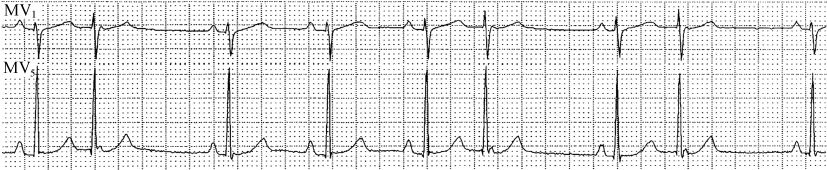
\includegraphics[width=5.58333in,height=1.14583in]{./images/Image00178.jpg}
 \captionsetup{justification=centering}
 \caption{房室交接性早搏的QRS波群后面始终跟随直立P波,提示为正相逆行P\textsuperscript{-}波}
 \label{fig11-18}
  \end{figure} 


3.发生机制

心房内的特殊传导纤维如结间束、James束及Kent束的存在为正相性逆行P\textsuperscript{-}波的解释提供了解剖学基础。当起源于房室交接区或心室异位激动经房室正道逆传受阻时,可从James束或从出口处位于心房上部的Kent束逆传,使心房除极顺序与窦性激动相似而出现直立P波,或房室交接区激动优先通过前结间束快速逆行到房间束和窦房交接区先激动心房上部,使心房除极顺序与窦性激动相似,也可出现直立P波。

\protect\hypertarget{text00018.htmlux5cux23subid150}{}{}

\section{室性早搏}

\protect\hypertarget{text00018.htmlux5cux23subid151}{}{}

\subsection{室性早搏的心电图特征}

(1)提早出现宽大畸形QRS-T波群,时间≥0.12s,T波方向与QRS主波方向相反。

(2)其前无相关的P波,其后偶有P\textsuperscript{-}波,R-P\textsuperscript{-} 间期<0.20s。

(3)多呈完全性代偿间歇,若有P\textsuperscript{-}波出现可呈不完全性代偿间歇。

\protect\hypertarget{text00018.htmlux5cux23subid152}{}{}

\subsection{室性早搏的定位诊断}

根据室性早搏QRS波形的特征来推测异位起搏点的部位,对于评估心室受损部位(如左心室受累时常出现左室型早搏,一般多严重)、为折返性室性早搏和室性心动过速的射频消融治疗提供参考等有一定的临床价值。

(1)高位室性早搏:起源于室间隔上部,希氏束分叉附近,提早出现的QRS波形与窦性略异,时间0.08~0.11s,其后可伴随逆行P\textsuperscript{-}波,R-P\textsuperscript{-}间期<0.20s,代偿间歇常完全。有时与房室交接性早搏伴非时相性心室内差异性传导难以鉴别(图\ref{fig11-19})。

\begin{figure}[!htbp]
 \centering
 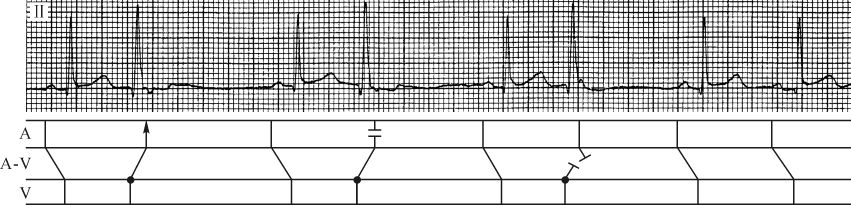
\includegraphics[width=5.75in,height=1.38542in]{./images/Image00179.jpg}
 \captionsetup{justification=centering}
 \caption{高位室性早搏二联律、有时伴逆传心房及房性融合波}
 \label{fig11-19}
  \end{figure} 

(2)右束支型或右室型室性早搏:起源于右束支近端,其QRS波形呈左束支阻滞图形;起源于右室壁的心肌中,其QRS波形类似左束支阻滞图形,即V\textsubscript{1}、V\textsubscript{2} 导联主波向下,Ⅰ、V\textsubscript{5}、V\textsubscript{6} 导联主波向上。

(3)左束支型或左室型室性早搏:起源于左束支近端,其QRS波形呈右束支阻滞图形;起源于左室壁的心肌中,其QRS波形类似右束支阻滞图形,即V\textsubscript{1}、V\textsubscript{2} 导联主波向上,Ⅰ、V\textsubscript{5}、V\textsubscript{6} 导联主波向下。

(4)左前分支型室性早搏:起源于左前分支近端,其QRS波形呈右束支阻滞图形伴电轴右偏。

(5)左后分支型室性早搏:起源于左后分支近端,其QRS波形呈右束支阻滞图形伴电轴左偏。

(6)心尖部室性早搏:亦称心室下部早搏,其QRS波形在Ⅱ、Ⅲ、aVF导联主波向下。

(7)心底部室性早搏:亦称心室上部早搏,其QRS波形在Ⅱ、Ⅲ、aVF导联主波向上。若起源于右心室流出道,其QRS波形除Ⅱ、Ⅲ、aVF导联主波向上外,胸前导联波形类似左束支阻滞图形。

(8)前壁部室性早搏:V\textsubscript{1} ~V\textsubscript{6}导联QRS主波均向下。

(9)后壁部室性早搏:V\textsubscript{1} ~V\textsubscript{6}导联QRS主波均向上。

(10)左心室侧壁部室性早搏:V\textsubscript{1} ~V\textsubscript{3}导联QRS主波向上,V\textsubscript{5} 、V\textsubscript{6}导联QRS主波向下。

\protect\hypertarget{text00018.htmlux5cux23subid153}{}{}

\subsection{特殊类型的室性早搏}

1.室性早搏QRS波形的变异

(1)多源性室性早搏:同一导联中至少有3种QRS波形且偶联间期不等的室性早搏(图\ref{fig11-20})。如呈两种形态、偶联间期不等的室性早搏,则称为双源性室性早搏。

\begin{figure}[!htbp]
 \centering
 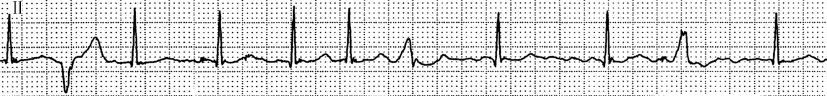
\includegraphics[width=5.58333in,height=0.64583in]{./images/Image00180.jpg}
 \captionsetup{justification=centering}
 \caption{风心病、心房颤动患者服用洋地黄过程中出现多源性室性早搏,提示洋地黄过量或中毒}
 \label{fig11-20}
  \end{figure} 

(2)多形性室性早搏:同一导联中室性早搏QRS波形不一,但偶联间期相等;表明传入径路只有一条,而传出径路有多条,其出口位置各异,但传至心室所需时间是相等的,类似房室结内倒Y型折返径路(图\ref{fig11-21})。

\begin{figure}[!htbp]
 \centering
 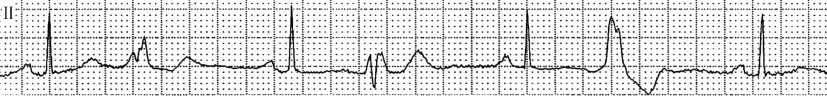
\includegraphics[width=5.58333in,height=0.64583in]{./images/Image00181.jpg}
 \captionsetup{justification=centering}
 \caption{多形性室性早搏二联律、间歇性T波改变}
 \label{fig11-21}
  \end{figure} 

(3)室性早搏伴心室内差异性传导:多发生在收缩中、晚期的同源性室性早搏,少数可发生在舒张早期。因遇及浦肯野纤维或心室肌的相对不应期而出现心室内差异性传导,其QRS波形较舒张期出现的室性早搏宽大畸形(图\ref{fig11-22})。

\begin{figure}[!htbp]
 \centering
 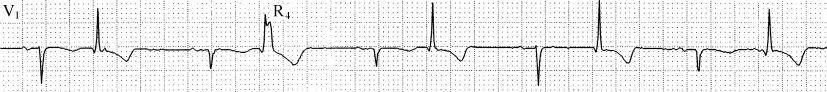
\includegraphics[width=5.58333in,height=0.61458in]{./images/Image00182.jpg}
 \captionsetup{justification=centering}
 \caption{并行性室性早搏二联律,有时伴心室内差异性传导(R\textsubscript{4})}
 \label{fig11-22}
  \end{figure} 


(4)特宽型室性早搏:室性早搏QRS波群时间>0.16s。多见于严重的器质性心脏病。其QRS波群愈宽,预后愈差。属病理性早搏。

(5)特矮型室性早搏:所有导联室性早搏QRS波幅均<1.0mV。属病理性早搏(图\ref{fig11-23})。

\begin{figure}[!htbp]
 \centering
 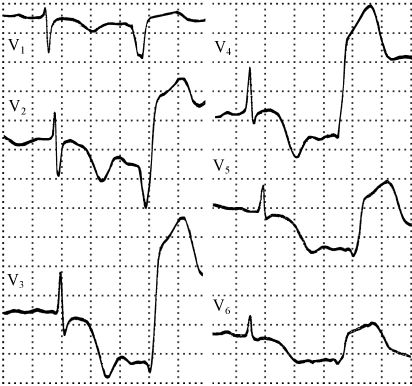
\includegraphics[width=2.78125in,height=2.60417in]{./images/Image00183.jpg}
 \captionsetup{justification=centering}
 \caption{胸痛患者,窦性搏动仅显示前间壁、前侧壁ST-T改变,而室性早搏却揭示了急性心肌梗死图形}
 \label{fig11-23}
  \end{figure} 

(6)平顶型室性早搏:室性早搏QRS波形类似于左束支阻滞时V\textsubscript{5}、V\textsubscript{6} 导联QRS波形的特征。属病理性早搏。

(7)室性融合波:舒张晚期室性早搏与窦性激动在心室内相融合而形成室性融合波,其P-R间期较窦性P-R间期短0~0.06s,形态介于室性早搏与窦性QRS波群之间。

(8)室性早搏揭示急性心肌梗死图形:极少数急性心肌梗死患者,基本的QRS-T波群形态正常,无异常Q波、ST段损伤型抬高和T波倒置,但在室性早搏QRS波群中却呈QR、QRs、qR型,ST段呈损伤型抬高伴T波高尖或倒置,显现急性心肌梗死的图形特征。可能由于基本节律时引起室间隔前下1/3左室面除极与左室游离壁除极时,其向量指向了左前方,使心肌梗死的波形特征被掩盖。当出现室性早搏引起心室非同步除极时,梗死图形才在室性早搏中充分显示出来。近年来发现室性早搏QRS波群呈QR、QRs、qR型也见于心肌病患者。从室性早搏QRS波群中诊断心肌梗死必须符合以下先决条件:①室性早搏QRS主波必须向上;②必须是以R波为主的导联,如V\textsubscript{5}、V\textsubscript{6} 导联等(图\ref{fig11-23})。

2.室性早搏偶联间期的变异

(1)特早型室性早搏:室性早搏的偶联间期<0.43s,包括T波上室性早搏(Ron-T现象),可伴有心室内差异性传导。当提早指数R-R′/Q-T<0.90时,易诱发严重的室性心律失常。

(2)特迟型室性早搏:室性早搏的偶联间期≥0.80s。此时室性早搏的频率≤75次/min,实为加速的室性逸搏。但由于基本节律太慢,与之相比,加速的逸搏即变为早搏。

(3)继发性室性早搏:亦称慢率性室性早搏,是指继发于长周期后的室性早搏,即该早搏仅在长R-R间期后出现,且有形成一系列室性二联律现象,室性早搏后代偿间歇又为下一个慢率性室性早搏创造条件,周而复始(图\ref{fig11-24})。

\begin{figure}[!htbp]
 \centering
 \includegraphics[width=5.58333in,height=1.1875in]{./images/Image00184.jpg}
 \captionsetup{justification=centering}
 \caption{MV\textsubscript{5}导联连续记录,定准电压0.5mV。显示窦性心动过缓伴室相性窦性心律不齐、继发性室性早搏,有时呈二联律及间位型、T波改变}
 \label{fig11-24}
  \end{figure} 


(4)偶联间期递增型室性早搏:亦称偶联间期文氏型室性早搏。室性早搏二联律时,其偶联间期逐渐延长,直至早搏消失,连续出现2~3次窦性搏动,周而复始。若连续出现3次窦性搏动,则为心室折返径路内交替性A型文氏周期(图\ref{fig11-25});若连续出现2次窦性搏动,则为折返径路内交替性B型文氏周期。

\begin{figure}[!htbp]
 \centering
 \includegraphics[width=5.67708in,height=1.38542in]{./images/Image00185.jpg}
 \captionsetup{justification=centering}
 \caption{室性早搏显性与隐性二联律、心室折返径路内交替性A型文氏周期(折返径路近端2:1阻滞、远端3:2文氏现象)}
 \label{fig11-25}
  \end{figure} 

(5)偶联间期递减型室性早搏:亦称偶联间期反向文氏型室性早搏。室性早搏二联律时,其偶联间期逐渐缩短,直至落到前一窦性搏动后的绝对不应期中而消失,以致连续出现2~3次窦性搏动,周而复始。前者为折返径路内交替性B型反向文氏周期,而后者则为折返径路内交替性A型反向文氏周期。

(6)偶联间期长、短交替型室性早搏:室性早搏二联律时,其偶联间期呈长、短交替或间歇性出现,系折返径路内快、慢径路传导所致(图\ref{fig11-26})。

\begin{figure}[!htbp]
 \centering
 \includegraphics[width=5.64583in,height=1.32292in]{./images/Image00186.jpg}
 \captionsetup{justification=centering}
 \caption{室性早搏二联律伴心室折返径路内双径路传导}
 \label{fig11-26}
  \end{figure} 

(7)偶联间期固定、R′波形一致,连续出现≥3次,且其R′-R′间期相等,形成短阵性室性心动过速:当折返激动沿着同一折返环路等速传导到达同一终点,并且周而复始地循环着,便可形成短阵性室性心动过速。

(8)偶联间期固定、R′波形一致,连续出现≥3次,但其R′-R′间期逐渐缩短或延长直至心动过速终止:当折返激动沿着同一折返径路折返时,其传导速度逐渐加快或减慢直至折返中断,周而复始,形成折返径路内反向文氏现象或文氏现象(图\ref{fig11-27})。

\begin{figure}[!htbp]
 \centering
 \includegraphics[width=5.66667in,height=1.54167in]{./images/Image00187.jpg}
 \captionsetup{justification=centering}
 \caption{窦性搏动、短阵性室性心动过速伴逆传心房及心室折返径路内5:4文氏现象}
 \label{fig11-27}
  \end{figure} 

3.隐匿性室性早搏二、三联律

这是一种持久的、连续的偶联间期固定型室性早搏二、三联律,并发间歇的、不定比例的传出阻滞。有以下两种类型:

(1)非间位型隐匿性室性早搏二、三联律:二联律时,室性早搏偶联间期固定,两个显性早搏之间夹有的窦性搏动数为奇数,即符合2n+1规律(n为自然数),代表隐匿性早搏的数目。三联律时,室性早搏偶联间期固定,两个显性早搏之间夹有的窦性搏动数为奇、偶数交替,即符合3n+2规律。

(2)间位型隐匿性室性早搏二、三联律:二联律时,符合1+(2n+1)规律;三联律时,符合1+(3n+2)规律。

4.舒张晚期室性早搏呈Ron-P现象

室性早搏QRS波群落在P波顶峰附近形成Ron-P现象,有学者认为室性早搏Ron-P现象较Ron-T现象更易诱发室性心动过速,但我们观察并非如此。

\protect\hypertarget{text00018.htmlux5cux23subid154}{}{}

\subsection{与插入性室性早搏有关的心律失常}

1.插入性室性早搏揭示房室结内双径路传导

窦性心动过缓时,适时的室性早搏仅逆传至房室交接区使其产生新的不应期,导致下一个窦性激动下传时出现P-R间期延长。该P-R间期延长有3种可能:①干扰性P-R间期延长,其R′-P间期与P-R间期呈反比关系;②通过房室结内慢径路传导,其P-R间期固定地延长,R′-P间期与P-R间期不呈反比关系矛盾现象;③上述两种情况兼而有之,较长的P-R间期略有互差,但互差<0.06s。

2.插入性室性早搏引起延期性代偿间歇

有3个特征:①窦性心动过缓时,适时出现插入性室性早搏;②插入性早搏后第1个窦性搏动的P-R间期明显地延长;③插入性早搏后第2个窦性搏动不能下传心室出现较长的R-R间期(图\ref{fig11-1})。

3.插入性室性早搏引发窦性反复搏动

插入性室性早搏后第1个窦性搏动的P-R间期延长,可引发窦性反复搏动,形成R′-P-QRSP\textsuperscript{-}-QRS的序列,其R-P\textsuperscript{-} 间期<P\textsuperscript{-}-R间期,且R-P\textsuperscript{-} 间期<0.08s。

\protect\hypertarget{text00018.htmlux5cux23subid155}{}{}

\subsection{室性早搏伴室房逆传情况}

1.室性早搏伴逆行隐匿性传导

所有室性早搏均会隐匿地逆传到房室交接区使其产生新的不应期,可绝对或相对地干扰下一个窦性激动的下传,出现完全性代偿间歇或无代偿间歇而呈插入性早搏。

2.室性早搏伴一度室房传导阻滞

室性早搏逆传心房大多发生在窦性心律较缓慢而偶联间期较短之时,因此时下一次窦性激动尚未传入心房,心房肌处于应激期,室性早搏逆传的激动方得以传入心房而产生逆行P\textsuperscript{-}波。若其R′-P\textsuperscript{-}间期>0.20s,则存在一度室房传导阻滞(图\ref{fig11-28})。

\begin{figure}[!htbp]
 \centering
 \includegraphics[width=5.58333in,height=0.90625in]{./images/Image00188.jpg}
 \captionsetup{justification=centering}
 \caption{窦性心动过缓、房性早搏、室性早搏伴室房逆传一度阻滞(R′-P\textsuperscript{-}间期0.25s)及两者形成的室性融合波(R\textsubscript{2} )}
 \label{fig11-28}
  \end{figure} 


3.室性早搏伴一度室房传导阻滞及房性融合波

室性早搏逆传心房时,其R′-P\textsuperscript{-}间期>0.20s,P\textsuperscript{-}波形态介于窦性P波与深倒逆行P\textsuperscript{-}波之间。需与室房逆传双径路伴心房双出口相鉴别,前者P\textsuperscript{-}波位置应是窦性P波预期出现部位,且P\textsuperscript{-}波形态易变,而后者R′-P\textsuperscript{-}间期有长、短两种,且互差≥0.06s,有两种固定形态的P\textsuperscript{-}波。

4.室性早搏逆传引起窦性节律重整

室性早搏逆传心房后再逆传至窦房结使其节律重整,出现不完全性代偿间歇。

5.室性早搏伴二度室房传导阻滞

室性早搏间歇性逆传心房产生逆行P\textsuperscript{-}波,故室性早搏QRS波群后面间歇性出现逆行P\textsuperscript{-} 波。

6.室性早搏伴室房逆传双径路

室性早搏的R′-P\textsuperscript{-}间期呈长、短两种,且互差≥0.06s,P\textsuperscript{-}波形态可异同(图\ref{fig36-6})。

7.室性早搏引发室性反复搏动或室性反复性心动过速

室性早搏逆传心房时,可沿房室交接区另一条径路再次下传心室,形成室性反复搏动,出现R′-P\textsuperscript{-}-QRS或R′-QRS的序列。反复搏动的QRS波形可正常或伴心室内差异性传导。若反复搏动连续出现≥3次,便形成室性反复性心动过速(图\ref{fig25-17})。

8.室性早搏引发房室折返性心动过速

适时的室性早搏经房室旁道逆传心房→房室正道→心室→房室旁道→心房,周而复始,形成顺向性房室折返性心动过速;若经房室正道逆传心房→房室旁道→心室→房室正道→心房,周而复始,则形成逆向型房室折返性心动过速而出现宽大畸形QRS波群。

9.室性早搏逆传引发非时相性心房内差异性传导

室性早搏代偿间歇后1个或数个窦性P波畸形。

10.室性早搏逆传心房引发房性逸搏

室性早搏逆传心房后可再逆传至窦房结使其节律重整,出现不完全性代偿间歇;也可与窦性激动在窦房交接区相干扰,出现完全性代偿间歇而引发房性逸搏(图\ref{fig11-29})。

\begin{figure}[!htbp]
 \centering
 \includegraphics[width=5.78125in,height=0.57292in]{./images/Image00189.jpg}
 \captionsetup{justification=centering}
 \caption{室性早搏三联律伴逆传心房及诱发房性逸搏(P\textsubscript{7} )}
 \label{fig11-29}
  \end{figure} 

\protect\hypertarget{text00018.htmlux5cux23subid156}{}{}

\subsection{室性早搏引发房性、房室交接性、室性逸搏}

室性早搏代偿间歇后可出现下级起搏点被动性发放冲动,形成房性、房室交接性或室性逸搏。

\protect\hypertarget{text00018.htmlux5cux23subid157}{}{}

\subsection{室性早搏诱发严重的心律失常}

Ron-T、Ron-P的室性早搏及成对室性早搏均可诱发室性心动过速、心室扑动或颤动而危及生命。

\protect\hypertarget{text00018.htmlux5cux23subid158}{}{}

\subsection{成对室性早搏QRS波形易变性的原因}

成对出现的室性早搏,其QRS波形有时变异性较大,有3种可能:①起源于两个部位的室性早搏;②起源于同一个部位,但第2个室性早搏出现心室内差异性传导;③室性早搏引发的室性反复搏动伴心室内差异性传导。

\protect\hypertarget{text00018.htmlux5cux23subid159}{}{}

\subsection{束支或分支性室性早搏与肌性室性早搏的心电图特征}

(1)束支或分支性室性早搏:起源于束支或分支起搏点的早搏,称为束支或分支性室性早搏。其QRS波形类似于束支或分支阻滞图形,QRS波群时间略增宽(<0.14s)或正常。

(2)肌性室性早搏:起源于浦肯野纤维或心室肌中起搏点的早搏,称为肌性室性早搏。其QRS波形不呈典型的束支或分支阻滞图形,QRS波群更宽大畸形(≥0.14s)。

\protect\hypertarget{text00018.htmlux5cux23subid160}{}{}

\subsection{室性早搏的分级}

Lown等将监护病房出现的室性早搏分为5级(表11-2),认为3~5级具有警报意义,易发生严重的室性心律失常而猝死。

\begin{table}[htbp]
\centering
\caption{室性早搏的Lown分级法}
\label{tab11-2}
\includegraphics[width=5.51042in,height=2.03125in]{./images/Image00190.jpg}
\end{table}

\protect\hypertarget{text00018.htmlux5cux23subid161}{}{}

\subsection{良性室性早搏与病理性室性早搏的鉴别}

室性早搏临床上非常多见,最好能判断该早搏是良性的还是病理性的。若是病理性的,是器质性心脏病所致,还是体液性异常所致(如药物中毒、电解质紊乱、酸碱平衡失调、低氧血症等),以利临床医生进一步诊治。良性与病理性室性早搏的鉴别见表11-3所示。

\begin{longtable}{c}
  \caption{良性室性早搏与病理性室性早搏的鉴别}
  \label{tab11-3}\\
  \endfirsthead
  \caption[]{良性室性早搏与病理性室性早搏的鉴别}
  \endhead
\includegraphics[width=\textwidth,height=\textheight,keepaspectratio]{./images/Image00191.jpg}\\
\includegraphics[width=\textwidth,height=\textheight,keepaspectratio]{./images/Image00192.jpg}
\end{longtable}

\section{房室旁道性早搏}

Kent束的慢旁道是由希-浦传导组织构成的,具有自律性。现已证明在旁道束纤维内或旁道束插入心房和心室的部位均易产生异位激动,所形成的早搏大多以并行节律点的性质单个出现,有时亦可形成异位心律。其心电图特征:①提早出现宽大畸形QRS-T波群,类似于既往预激波形,但更宽,表现为完全性预激波形特征。②其QRS波群前后可有逆行P\textsuperscript{-}波或逆行P\textsuperscript{-}波重叠在QRS波群之中或无逆行P\textsuperscript{-}波,这取决于该早搏激动有无逆传心房或逆传与前传的时间差;若逆传快于前传,则逆行P\textsuperscript{-}波出现在QRS波群之前,此时与心房下部早搏伴完全性预激难以鉴别;若逆传与前传分别同时到达心房和心室,则逆行P\textsuperscript{-}波重叠在QRS波群之中;若逆传慢于前传,则逆行P\textsuperscript{-}波出现在QRS波群之后。③有完全或不完全性代偿间歇。

\protect\hypertarget{text00018.htmlux5cux23subid163}{}{}

\section{早搏波形正常化}

\protect\hypertarget{text00018.htmlux5cux23subid164}{}{}

\subsection{基本概念}

当窦性心律或房室交接性心律伴有单侧束支阻滞或预激综合征时,如发生室性或室上性早搏,其QRS波形反而变窄,与正常QRS波群相似,则称为早搏波形正常化。其正常化的程度可以是较束支阻滞时的宽度减轻(轻度正常化)、接近于正常范围(显著正常化)或波形完全正常(完全正常化)。

\protect\hypertarget{text00018.htmlux5cux23subid165}{}{}

\subsection{早搏波形正常化类型(以窦性心律为例)}

1.窦性心律伴单侧束支阻滞并发早搏波形正常化

凡是能使左、右心室同步除极(<25ms)的早搏,均可出现正常QRS波形,有以下8种情况:

(1)起源于束支阻滞区下方且距左、右束支的距离大致相等的室间隔型早搏。

(2)同侧性舒张晚期室性早搏与窦性激动形成室性融合波。

(3)功能性单侧束支阻滞并发收缩晚期房性早搏伴对侧束支3相性阻滞。

(4)功能性单侧束支阻滞并发收缩晚期房室交接性早搏伴对侧束支3相性阻滞。

(5)功能性单侧束支阻滞并发房性或房室交接性早搏伴同侧束支超常期传导(图\ref{fig11-30})。

\begin{figure}[!htbp]
 \centering
 \includegraphics[width=5.58333in,height=1.1875in]{./images/Image00193.jpg}
 \captionsetup{justification=centering}
 \caption{V\textsubscript{1}导联连续记录,显示完全性右束支阻滞(功能性阻滞)、频发房性早搏,其中部分房性早搏QRS波形正常化(R\textsubscript{3}、R\textsubscript{10} 、R\textsubscript{18} )}
 \label{fig11-30}
  \end{figure} 


(6)束支阻滞属4相性阻滞,并发房性或房室交接性早搏可呈正常QRS波形。

(7)右束支阻滞时,房性早搏伴B型预激综合征,使左、右心室同步除极。

(8)左束支阻滞时,房性早搏伴A型预激综合征,左束支阻滞图形被掩盖。

2.窦性心律伴预激综合征并发早搏波形正常化

(1)预激综合征并发适时的房性早搏:当房室旁道存在3相性阻滞时,适时的房性早搏便通过房室正道下传,且不发生心室内差异性传导,便会出现正常QRS波形。

(2)预激综合征并发房室交接性早搏:舒张中期房室交接性早搏沿正常途径下传心室,且不伴心室内差异性传导时,便会出现正常QRS波形;舒张晚期早搏则有可能与预激QRS波群形成室性融合波而正常化。

(3)预激综合征并发室性早搏波形正常化:起源于高位室间隔部位的舒张早、中期室性早搏,起搏点距房室束分叉处较近,几乎以相等速度沿左、右束支下传,同步激动心室,产生正常QRS波形;舒张晚期室性早搏也有可能与预激QRS波群形成室性融合波而正常化。

\protect\hypertarget{text00018.htmlux5cux23subid166}{}{}

\section{高风险的早搏}

早搏在临床上非常多见,有的患者呈二、三联律出现,24h内多达数万次而安全无恙,而有的患者早搏数量虽然很少,但其诱发的严重心律失常却能致人于死地,故有必要在此探讨高风险的早搏。

\protect\hypertarget{text00018.htmlux5cux23subid167}{}{}

\subsection{高风险的房性早搏及其心律失常}

(1)阻滞型房性早搏二联律、成对出现的阻滞型房性早搏三联律引发心动过缓:若患者本身就存在窦性心动过缓,则出现上述心律失常时,由于房性早搏对窦性节律的重整,将产生较长的R-R间歇,导致心排血量减少,血压降低。

(2)房性早搏诱发窦性停搏:在窦房结功能低下时,房性早搏重整窦性节律后,可抑制其激动的发放,引发窦性停搏;若下级起搏点功能不良,则会引发较长时间的全心停搏。

(3)房性早搏诱发快速性房性心律失常:较多见,偶联间期为0.20~0.30s的房性早搏,易落在心房易颤期内而诱发房性心动过速、心房颤动或心房扑动等快速性房性心律失常。

(4)快速性房性心律失常终止后诱发窦性停搏:阵发性心房颤动、心房扑动、房性心动过速等快速性心律失常发作终止时,在恢复正常窦性心律之前,出现长R-R间歇(多由窦性停搏、高度窦房传导阻滞及严重的窦性心动过缓等所致),可引起一过性急性脑缺血,出现晕厥、阿-斯综合征发作,甚至猝死。

(5)房性早搏诱发阵发性三度房室传导阻滞:阻滞型房性早搏、房性心动过速代偿间歇后,可诱发4相性阵发性三度房室传导阻滞。阵发性三度房室传导阻滞,无论与频率快慢是否相关,其阻滞部位大多发生在希氏束或希氏束以下(束支、分支内),多伴随低位逸搏点冲动形成障碍,不能及时发放冲动而出现较长时间的心室停搏,导致晕厥或阿-斯综合征发作而危及生命(图\ref{fig11-14})。

(6)房性早搏诱发极速型房室、房室结内折返性心动过速:当患者存在房室旁道或房室结内双径路传导时,适时的房性早搏可诱发极速型房室、房室结内折返性心动过速(心室率>200~250次/min),将导致心排血量减少、心肌耗氧量增加,易恶化为心室颤动而危及生命。

(7)多源性房性早搏诱发紊乱性房性心动过速:由多个心房内异位起搏点发放的极不稳定的激动所形成的多源性自律性异常,常以频发性、多源性房性早搏为主体组成多波形、极不规则而快速的心律,称为紊乱性房性心动过速,有的可发展为心房颤动,故又称为颤动前心律。多发生在老年慢性肺心病患者,尤其是伴有难治性心力衰竭的重症患者,常发展为心房颤动,病死率高。其心电图特征:①至少有发自3个不同的房性异位灶的P′波出现在同一导联上,P′波的形态不同,P′-P′间期不等,P′-R间期长短不一;②心房率100~250次/min;③P′波与P′波之间有等电位线;④心房率、心室率快而不规则;⑤无起止突然的特点。

\protect\hypertarget{text00018.htmlux5cux23subid168}{}{}

\subsection{高风险的室性早搏及其心律失常}

(1)各种病理性室性早搏:①多源性、多形性室性早搏;②特宽型室性早搏;③特矮型室性早搏;④平顶型室性早搏;⑤心肌梗死型室性早搏:以R波为主导联室性早搏QRS波群呈QR、QRs、qR型,ST段呈损伤型抬高伴T波高尖或倒置,显现急性心肌梗死的图形特征。

(2)特早型室性早搏,即Ron-T现象:室性早搏的偶联间期<0.43s,包括T波上室性早搏(Ron-T现象)或提早指数R-R′/Q-T<0.90时,易诱发严重的室性心律失常而猝死。

(3)发生在严重器质性心脏病的室性早搏:①急性心肌梗死;②各类心肌病,如扩张型、肥厚型、致心律失常性右室心肌病等,由于患者心脏扩大、心功能减退,绝大多数会出现复杂性、顽固性、难治性室性心律失常,易引发恶性心律失常而猝死。

(4)发生在电解质严重紊乱的室性早搏:①严重的低钾血症(<3.0mmon/L):导致心肌细胞自律性和兴奋性增高、传导速度减慢引起传导阻滞、心室内折返及早期后除极而引发室性心律失常,以多源性、多形性室性早搏、短阵性室性心动过速多见,有时出现尖端扭转型室性心动过速等恶性室性心律失常;②严重的高钾血症(>10mmol/L):QRS波群与T波融合形成正弦曲线,频率缓慢而不规则,Q-T间期延长,直至出现心脏停搏或心室扑动、颤动而死亡。

(5)发生在长Q-T间期综合征的室性早搏:早搏易落在心室易颤期内而引发尖端扭转型室性心动过速、心室颤动而猝死。

(6)发生在短Q-T间期综合征的室性早搏:Q-T间期短至0.22~0.29s时,早搏易诱发室性心动过速、心室颤动而猝死。

(7)发生在异常J波综合征的室性早搏:异常J波与恶性室性心律失常有密切关系。

(8)发生在Brugada综合征的室性早搏。

(9)发生在Lambda波(λ波)的室性早搏。

(10)发生在T波电交替的室性早搏:有T波电交替者,发生致命性室性心律失常的危险性增加14倍,故T波电交替已成为识别高危患者的一个重要而非常直观的指征。

(11)药物过量或中毒引起的室性早搏:①洋地黄中毒:出现频发多形性或多源性室性早搏二联律、室性心动过速及双向性室性心动过速等,其中后两者死亡率高达68\%~100\%;②胺碘酮:剂量过大时,因Q-T间期延长,心室复极离散度增加,所产生的室性早搏可引起扭转型室性心动过速、心室颤动而猝死;③普罗帕酮:剂量过大或毒性作用时,所产生的室性早搏可引起多形性或尖端扭转型室性心动过速及心室颤动等。

\protect\hypertarget{text00019.html}{}{}

\protect\hypertarget{text00019.htmlux5cux23chapter19}{}{}

\chapter{逸搏和逸搏心律}

\protect\hypertarget{text00019.htmlux5cux23subid169}{}{}

\section{概 述}

当心脏主导节律(通常为窦房结)发放激动的频率过慢(心动过缓)、激动形成异常(停搏)或激动传导异常(窦房、房室传导阻滞)时,下级潜在的起搏点将被动地发放冲动,免遭心脏停搏过久,这是一种生理性代偿机制。若下级潜在起搏点偶尔被动地发出1~2次激动,则称为逸搏;若下级潜在起搏点连续发出≥3次激动,则称为逸搏心律。

\protect\hypertarget{text00019.htmlux5cux23subid170}{}{}

\subsection{逸搏和逸搏心律的分类}

(1)根据起搏点的部位:分为窦性、房性、房室交接性、室性和房室旁道性逸搏5种类型,其中以房室交接性逸搏、室性逸搏多见。

(2)根据逸搏频率的快慢:分为过缓的逸搏和过缓的逸搏心律、逸搏和逸搏心律、加速的逸搏和加速的逸搏心律。

(3)根据逸搏起搏点的多少:分为单源性、双源性和多源性逸搏。

\protect\hypertarget{text00019.htmlux5cux23subid171}{}{}

\subsection{逸搏和逸搏心律的共同特征}

(1)逸搏周期固定:凡起源于同一起搏点的逸搏,无论是散在的,还是连续出现的逸搏心律,其逸搏周期多是固定的。这一特征有助于发现散在的逸搏,特别是在复杂的心律失常中。

(2)延迟出现:逸搏必然是延迟出现的,逸搏周期一定大于主导节律的基本周期。

(3)可有起步现象或温醒现象:逸搏起搏点的节律通常是规则的,有时在开始建立逸搏心律时,最初的几个逸搏周期往往略长,频率略慢,以后频率逐渐加快直至固定。表明下级起搏点从主导节律抑制下脱逸出来后,建立其自身起搏点需要一个短暂的准备过程,然后才能逐渐恢复而达到稳定,这种现象称为起步现象或温醒现象。

(4)无传入阻滞保护:逸搏或逸搏心律是由于主导节律的激动形成异常或传导异常而引起下级潜在的起搏点被动地发放激动,一旦主导节律又能较快地发放激动或下传时,逸搏或逸搏心律即可消失。

\protect\hypertarget{text00019.htmlux5cux23subid172}{}{}

\subsection{临床意义}

逸搏和逸搏心律与房室超常期传导、韦金斯基现象是免遭心脏停搏过久的3种生理性代偿机制,具有保护作用。由于逸搏和逸搏心律都是继发的,必须寻找发生逸搏和逸搏心律的始发原因,如心动过缓、停搏、传导阻滞等。逸搏的出现常使心电图改变复杂化,影响心律失常的分析和诊断。

\protect\hypertarget{text00019.htmlux5cux23subid173}{}{}

\section{窦性逸搏和逸搏心律}

\protect\hypertarget{text00019.htmlux5cux23subid174}{}{}

\subsection{心电图特征}

(1)在两阵快速或较快速异位性心动过速终止后间歇期内,略为延迟出现1~2次窦性搏动,其P波形态与正常窦性P波完全相同。

(2)若逸搏周期0.60~1.0s,频率60~100次/min,则称为窦性逸搏;若逸搏周期>1.0s,频率<60次/min,则称为过缓的窦性逸搏(图\ref{fig12-1})。

\begin{figure}[!htbp]
 \centering
 \includegraphics[width=5.79167in,height=0.55208in]{./images/Image00194.jpg}
 \captionsetup{justification=centering}
 \caption{短阵性不纯性心房扑动终止后出现过缓的窦性逸搏}
 \label{fig12-1}
  \end{figure} 

(3)若连续出现≥3次窦性逸搏,则称为窦性逸搏心律,亦称为正常的窦性心律

\protect\hypertarget{text00019.htmlux5cux23subid175}{}{}

\subsection{临床意义}

(1)窦性逸搏的出现,仍然标志着窦房结有正常的起搏功能,出现窦性逸搏是由于下级起搏点发放快速或较快速激动后又突然终止所致。若异位节律点得到控制后,将自然恢复正常的窦性心律。

(2)过缓的窦性逸搏常见于窦房结自律性降低或病窦综合征患者,异位性心动过速终止及转复为窦性心律后,可出现窦性停搏。

\protect\hypertarget{text00019.htmlux5cux23subid176}{}{}

\section{房性逸搏和逸搏心律}

\protect\hypertarget{text00019.htmlux5cux23subid177}{}{}

\subsection{心电图特征}

(1)在两阵窦性心律或两阵异位心律之间,延迟出现1~2次P′波或P′-QRS-T波群,P′波形态与窦性P波不同。P′波形态一致者,称为单源性房性逸搏;P′波呈两种形态者,称为双源性房性逸搏(图\ref{fig12-2});P′波形态≥3种者,称为多源性房性逸搏

\begin{figure}[!htbp]
 \centering
 \includegraphics[width=5.78125in,height=0.83333in]{./images/Image00195.jpg}
 \captionsetup{justification=centering}
 \caption{上、下两行系MV\textsubscript{1}导联同时不连续记录,病窦综合征(慢-快型综合征)患者出现窦性停搏或显著的窦性心动过缓、过缓的双源性房性逸搏(上行P\textsubscript{2} ,但P\textsubscript{2} 波不能除外房性融合波;下行P\textsubscript{5} )、过缓的窦性逸搏(下行P\textsubscript{6} )、短阵性房性心动过速}
 \label{fig12-2}
  \end{figure} 


(2)若逸搏周期1.0~1.20s,频率50~60次/min,则称为房性逸搏;若逸搏周期>1.20s,频率<50次/min,则称为过缓的房性逸搏;若逸搏周期0.60~1.0s,频率61~100次/min,则称为加速的房性逸搏。

(3)若连续延迟出现≥3次P′-QRS-T波群,则称为过缓的房性逸搏心律(<50次/min)、房性逸搏心律(50~60次/min)或加速的房性逸搏心律(61~100次/min)(图\ref{fig12-3}、图\ref{fig12-4})。

\begin{figure}[!htbp]
 \centering
 \includegraphics[width=5.58333in,height=0.57292in]{./images/Image00196.jpg}
 \captionsetup{justification=centering}
 \caption{病窦综合征患者出现窦性心动过缓、房性逸搏心律(P\textsubscript{3}~P\textsubscript{6} )}
 \label{fig12-3}
  \end{figure} 


\begin{figure}[!htbp]
 \centering
 \includegraphics[width=5.58333in,height=0.65625in]{./images/Image00197.jpg}
 \captionsetup{justification=centering}
 \caption{加速的房性逸搏心律(起源于心房下部,频率92次/min)}
 \label{fig12-4}
  \end{figure} 

(4)P′-R间期、QRS波形与窦性一致,有时房性逸搏P′波刚刚出现时,又发生了房室交接性逸搏或室性逸搏,则P′-R间期<0.12s,P′波被干扰而未能下传。

(5)有时可见延迟出现的P′波与窦性P波相融合的房性融合波。

(6)可有起步现象或温醒现象。

\protect\hypertarget{text00019.htmlux5cux23subid178}{}{}

\subsection{房性逸搏的定位诊断}

请见第十一章第四节房性早搏的定位诊断。

\protect\hypertarget{text00019.htmlux5cux23subid179}{}{}

\subsection{鉴别诊断}

1.与窦性逸搏伴非时相性心房内差异性传导的鉴别

两者有时较难鉴别。窦性逸搏伴非时相性心房内差异性传导多见于房性早搏、能逆传心房的房室交接性早搏及室性早搏的代偿间歇之后,若连续出现2次者,则第2个逸搏周期与窦性基本周期一致。

2.房性逸搏伴房性融合波与多源性房性逸搏的鉴别

两者的P′波形态多变,但前者的逸搏周期多固定,而后者的逸搏周期却长短不一。

\protect\hypertarget{text00019.htmlux5cux23subid180}{}{}

\subsection{临床意义}

房性逸搏及其逸搏心律的出现,表明心脏有潜在的逸搏起搏能力,它本身并无重要临床意义,主要取决于原发性心律失常。而加速的房性逸搏及其逸搏心律的出现,若不伴有窦性心律竞争,则说明窦房结自律性降低,部分见于器质性心脏病,如冠心病、病窦综合征等,部分则无器质性心脏病;若伴有窦房结-心房节律竞争,则见于心肌炎、急性心肌梗死、洋地黄中毒及心脏手术等。

\protect\hypertarget{text00019.htmlux5cux23subid181}{}{}

\section{房室交接性逸搏和逸搏心律}

\protect\hypertarget{text00019.htmlux5cux23subid182}{}{}

\subsection{心电图特征}

(1)延迟出现1~2次QRS-T波群,其形态与主导节律QRS-T波群(预激综合征除外)一致或略有差异,后者为伴有非时相性心室内差异性传导。

(2)其QRS波群前、中、后可有逆行P\textsuperscript{-}波,其P\textsuperscript{-} -R间期<0.12s、R-P\textsuperscript{-}间期<0.16s;或始终无逆行P\textsuperscript{-}波,而出现窦性P波,但P-R间期<0.12s,表明P波被干扰而不能下传(图\ref{fig12-5})。

\begin{figure}[!htbp]
 \centering
 \includegraphics[width=5.58333in,height=0.60417in]{./images/Image00198.jpg}
 \captionsetup{justification=centering}
 \caption{病窦综合征患者出现显著的窦性心动过缓、过缓的房室交接性逸搏心律(R\textsubscript{1}~R\textsubscript{3} )}
 \label{fig12-5}
  \end{figure} 


(3)若逸搏周期1.0~1.5s,频率40~60次/min,则称为房室交接性逸搏;若逸搏周期>1.5s,频率<40次/min,则称为过缓的房室交接性逸搏;若逸搏周期0.6~1.0s,频率61~100次/min,则称为加速的房室交接性逸搏。

(4)若连续延迟出现≥3次QRS-T波群,则称为房室交接性逸搏心律(40~60次/min)、过缓的房室交接性逸搏心律(<40次/min)或加速的房室交接性逸搏心律(61~100次/min,图\ref{fig12-6})。

\begin{figure}[!htbp]
 \centering
 \includegraphics[width=5.58333in,height=0.65625in]{./images/Image00199.jpg}
 \captionsetup{justification=centering}
 \caption{低钾血症患者(血钾3.1mol/L)出现加速的房室交接性逸搏心律}
 \label{fig12-6}
  \end{figure} 

(5)有时可见房性融合波,偶见窦性激动与房室交接性逸搏所形成的窦-交室性融合波。

(6)可有起步现象或温醒现象。

(7)双源性或多源性房室交接性逸搏少见,可从QRS波形、频率及逆行P\textsuperscript{-}波出现位置加以分辨(图\ref{fig12-7}、图\ref{fig12-8})。

\begin{figure}[!htbp]
 \centering
 \includegraphics[width=5.58333in,height=1.70833in]{./images/Image00200.jpg}
 \captionsetup{justification=centering}
 \caption{V\textsubscript{3}导联连续记录,风心病、心房颤动患者,服用洋地黄过程中出现三度房室传导阻滞、过缓的双源性房室交接性逸搏及其心律(频率34次/min),其中一源伴非时相性心室内差异性传导(R\textsubscript{2} 、R\textsubscript{6} 、R\textsubscript{8} ),并可见交-交室性融合波(R\textsubscript{7} ),提示洋地黄中毒}
 \label{fig12-7}
  \end{figure} 


\begin{figure}[!htbp]
 \centering
 \includegraphics[width=5.76042in,height=2.84375in]{./images/Image00201.jpg}
 \captionsetup{justification=centering}
 \caption{Ⅱ导联连续记录,显示窦性停搏、多源性房室交接性逸搏心律伴外出二度阻滞或停搏(R\textsubscript{1}~R\textsubscript{3} 为一源,R\textsubscript{4} ~R\textsubscript{10}为一源,R\textsubscript{11} ~R\textsubscript{14}为一源),其中一源表现为加速的逸搏心律(61~62次/min)}
 \label{fig12-8}
  \end{figure} 



\protect\hypertarget{text00019.htmlux5cux23subid183}{}{}

\subsection{非时相性心室内差异性传导的心电图特征及其发生机制}

1.心电图特征

延迟出现的QRS波形与窦性稍有差异,主要表现为起始向量不一致、R波振幅略有高低或S波略有深浅,但时间多在正常范围内(图\ref{fig12-9});频率多在40~60次/min,亦有<40次/min或>60次/min者。

\begin{figure}[!htbp]
 \centering
 \includegraphics[width=5.58333in,height=0.66667in]{./images/Image00202.jpg}
 \captionsetup{justification=centering}
 \caption{窦性停搏、房性逸搏(P\textsubscript{3})、房性融合波(P\textsubscript{5})、房室交接性逸搏伴非时相性心室内差异性传导(R\textsubscript{3} )}
 \label{fig12-9}
  \end{figure} 


2.发生机制

主要与房室交接性逸搏起搏点的位置及其下传的途径有关。

(1)逸搏起搏点位于房室束(希氏束)分叉部的近端。

(2)逸搏起搏点来源于心室分支。

(3)逸搏起搏点位于房室交接区的边缘区或下部,激动沿着房室交接区、希氏束内解剖上或功能上纵向分离的径路下传,首先通过希氏束的一部分传导纤维到达心室肌的特定部位使其提早除极,尔后再通过浦肯野纤维快速传导径路到达心室的其他部分,导致逸搏QRS波群形态与窦性不一致,但时间仍在正常范围。

(4)逸搏起搏点的激动通过异常传导径路下传心室,如Mahaim纤维。

\protect\hypertarget{text00019.htmlux5cux23subid184}{}{}

\subsection{鉴别诊断}

1.与心房下部逸搏的鉴别

若P\textsuperscript{-}波位于QRS波群之前的房室交接性逸搏应与心房下部逸搏相鉴别,前者P\textsuperscript{-}-R间期<0.12s,而后者P\textsuperscript{-} -R间期≥0.12s。

2.房室交接性逸搏伴非时相性心室内差异性传导与高位室性逸搏的鉴别

高位室性逸搏又称为室间隔性逸搏,指异位起搏点起源于室间隔的上部(希氏束分叉处),激动经正常径路沿左、右束支下传,其QRS波群形态、时间酷似室上性,与房室交接性逸搏伴非时相性心室内差异性传导有时很难鉴别,表12-1可能有助于两者的鉴别。

\begin{table}[htbp]
\centering
\caption{房室交接性逸搏伴非时相性心室内差异性传导与高位室性逸搏的鉴别}
\label{tab12-1}
\includegraphics[width=6.22917in,height=1.8125in]{./images/Image00203.jpg}
\end{table}

3.心房颤动时房室交接性逸搏的识别

在同一份心电图上(记录1min)有3个以上1.0~1.5s等长的R-R间期,可提示房室交接性逸搏;若伴有非时相性心室内差异性传导,则较容易识别(图\ref{fig12-10})。

\begin{figure}[!htbp]
 \centering
 \includegraphics[width=5.58333in,height=1.27083in]{./images/Image00204.jpg}
 \captionsetup{justification=centering}
 \caption{MV\textsubscript{1} 、MV\textsubscript{5}导联同步记录,显示心房颤动伴缓慢的心室率、房室交接性逸搏伴非时相性心室内差异性传导(R\textsubscript{2}、R\textsubscript{4}),提示二度房室传导阻滞、不完全性右束支阻滞、轻度ST段改变、Q-T间期延长}
 \label{fig12-10}
  \end{figure} 


\protect\hypertarget{text00019.htmlux5cux23subid185}{}{}

\subsection{临床意义}

正常频率的房室交接性逸搏及其心律本身是一种生理性保护机制,其预后则取决于形成逸搏的原因,如三度房室传导阻滞时出现的逸搏较窦性心动过缓时出现的逸搏要差;过缓的房室交接性逸搏及其心律,表明房室交接区起搏点受到抑制或自律性降低,可能需要安装人工起搏器;加速的房室交接性逸搏及其心律,表明房室交接区起搏点自律性增高,见于心肌炎、急性心肌梗死、洋地黄中毒及心脏手术等。

\protect\hypertarget{text00019.htmlux5cux23subid186}{}{}

\section{室性逸搏和逸搏心律}

\protect\hypertarget{text00019.htmlux5cux23subid187}{}{}

\subsection{心电图特征}

(1)延迟出现1~2次宽大畸形QRS-T波群,QRS时间≥0.12s,T波与QRS主波方向相反。若QRS波形一致,则为单源性室性逸搏(图\ref{fig12-11});若QRS波形呈两种形态,则为双源性室性逸搏(图\ref{fig12-12});若QRS波形≥3种形态,则为多源性室性逸搏(图\ref{fig12-13})。

\begin{figure}[!htbp]
 \centering
 \includegraphics[width=5.82292in,height=0.875in]{./images/Image00205.jpg}
 \captionsetup{justification=centering}
 \caption{高血压病、脑血管意外患者在心肺复苏过程中出现窦性停搏、过缓的房室交接性逸搏((R\textsubscript{1}、R\textsubscript{3} 、R\textsubscript{5})、室性逸搏(R\textsubscript{2} 、R\textsubscript{4} )}
 \label{fig12-11}
  \end{figure} 


\begin{figure}[!htbp]
 \centering
 \includegraphics[width=5.58333in,height=0.75in]{./images/Image00206.jpg}
 \captionsetup{justification=centering}
 \caption{心肺复苏过程中出现窦性停搏、由加速的双源性室性逸搏(R\textsubscript{3}、R\textsubscript{5} 、R\textsubscript{7})及双源性室性早搏组成的室性异位心律}
 \label{fig12-12}
  \end{figure} 


\begin{figure}[!htbp]
 \centering
 \includegraphics[width=5.58333in,height=0.75in]{./images/Image00207.jpg}
 \captionsetup{justification=centering}
 \caption{冠心病患者出现三度房室传导阻滞、多源性加速的室性逸搏及其心律、室性融合波(R\textsubscript{4})}
 \label{fig12-13}
  \end{figure} 


(2)其QRS波群前、中、后可有窦性P波,但P-R间期<0.12s,表明P波被干扰而不能下传;或QRS波群后面可有逆行P\textsuperscript{-}波,其R′-P\textsuperscript{-} 间期<0.20s。

(3)若逸搏周期1.5~3.0s,频率20~40次/min,则称为室性逸搏;若逸搏周期>3.0s,频率<20次/min,则称为过缓的室性逸搏;若逸搏周期0.60~1.50s,频率41~100次/min,则称为加速的室性逸搏。其逸搏周期可稍不规则。

(4)若连续延迟出现≥3次宽大畸形的QRS-T波群,则称为室性逸搏心律(20~40次/min)、过缓的室性逸搏心律(<20次/min)或加速的室性逸搏心律(41~100次/min,图\ref{fig12-14})。

(5)可有室性融合波。

(6)可有起步现象或温醒现象。

\begin{figure}[!htbp]
 \centering
 \includegraphics[width=5.5625in,height=0.59375in]{./images/Image00208.jpg}
 \captionsetup{justification=centering}
 \caption{风心病、心房颤动患者。服用洋地黄过程中出现三度房室传导阻滞、加速的室性逸搏心律(频率49次/min)或房室交接性逸搏心律伴完全性右束支阻滞、符合洋地黄中毒的心电图表现}
 \label{fig12-14}
  \end{figure} 

\protect\hypertarget{text00019.htmlux5cux23subid188}{}{}

\subsection{室性逸搏的定位诊断}

请见第十一章第六节室性早搏的定位诊断。

\protect\hypertarget{text00019.htmlux5cux23subid189}{}{}

\subsection{临床意义}

出现室性逸搏及其逸搏心律,虽然其本身是一种生理性保护机制,但表明窦房结、心房、房室交接区起搏点均受到了抑制或出现房室传导阻滞,常见于严重的心脏病患者。由于室性逸搏起搏点的自律性极不稳定,易发生停搏,导致心室停搏,故属严重心律失常的范畴,应及时安装人工起搏器。加速的室性逸搏及其心律,表明室性起搏点自律性增高,见于心肌炎、急性心肌梗死、洋地黄中毒、心肌再灌注损伤及心脏手术后等,但一般不会转为心室颤动。

\protect\hypertarget{text00019.htmlux5cux23subid190}{}{}

\section{房室旁道性逸搏和逸搏心律}

1.心电图特征

(1)延迟出现1~2次宽大畸形QRS-T波群,类似于既往预激综合征时QRS-T波群,但更宽,表现为完全性预激波形特征。

(2)其QRS波群前、中、后可有逆行P\textsuperscript{-}波或无逆行P\textsuperscript{-} 波,若逆行P\textsuperscript{-}波位于QRS波之前,其P\textsuperscript{-}-R间期<0.12s,与心房下部逸搏伴完全性预激难以鉴别。

(3)逸搏周期1.0~1.5s,频率40~60次/min。

(4)若连续延迟出现≥3次宽大畸形QRS-T波群,则称为房室旁道性逸搏心律(40~60次/min)或加速的房室旁道性逸搏心律(61~100次/min)。

2.鉴别诊断

主要与室性逸搏及其逸搏心律相鉴别。若逸搏QRS波形与预激综合征时QRS波形相似或更宽,则首先考虑为房室旁道性逸搏。

3.临床意义

房室旁道性逸搏的出现,表明房室旁道传导组织具有潜在的起搏功能。

\protect\hypertarget{text00020.html}{}{}

\protect\hypertarget{text00020.htmlux5cux23chapter20}{}{}

\chapter{经典的扑动、颤动及其进展}

\protect\hypertarget{text00020.htmlux5cux23subid191}{}{}

\section{经典的心房扑动及其进展}

心房扑动是介于房性心动过速与心房颤动之间的一种快速而规则的房性心律失常。其心房波表现为形态、方向、振幅和间距完全一致类似三角形锯齿波或波浪样的扑动波,波间无等电位线,频率多在251~430次/min,有时可慢至160次/min,称为F波。

\protect\hypertarget{text00020.htmlux5cux23subid192}{}{}

\subsection{分型}

1.根据F波的频率、在Ⅱ、Ⅲ、aVF导联的形态、极性,分为Ⅰ、Ⅱ型

(1)Ⅰ型心房扑动:又称为常见型(典型)心房扑动,F波频率251~350次/min,在Ⅱ、Ⅲ、aVF导联呈负向锯齿波,锐角尖端向下,射频消融术能终止心房扑动的发作(图\ref{fig13-1})。

\begin{figure}[!htbp]
 \centering
 \includegraphics[width=5.58333in,height=0.42708in]{./images/Image00209.jpg}
 \captionsetup{justification=centering}
 \caption{Ⅰ型心房扑动伴正常心室率,房室呈4:1传导}
 \label{fig13-1}
  \end{figure} 

(2)Ⅱ型心房扑动:又称为少见型心房扑动,F波频率350~430次/min,在Ⅱ、Ⅲ、aVF导联呈较圆钝锯齿波,凸面向上,射频消融术效果不理想(图\ref{fig13-2})。

\begin{figure}[!htbp]
 \centering
 \includegraphics[width=5.58333in,height=0.48958in]{./images/Image00210.jpg}
 \captionsetup{justification=centering}
 \caption{Ⅱ型心房扑动伴正常心室率,房室呈4:1传导}
 \label{fig13-2}
  \end{figure} 

2.根据F波形态的易变性,分为4种类型

(1)尖端扭转型心房扑动:F波尖端方向围绕基线扭转,周而复始,如同尖端扭转型室性心动过速(图\ref{fig13-3})。

\begin{figure}[!htbp]
 \centering
 \includegraphics[width=5.58333in,height=0.77083in]{./images/Image00211.jpg}
 \captionsetup{justification=centering}
 \caption{V\textsubscript{1}导联连续记录,尖端扭转型心房扑动伴长R-R间期(2.21~2.38s,房室呈4:1~12:1传导),提示存在二度房室传导阻滞}
 \label{fig13-3}
  \end{figure} 


(2)不纯性心房扑动:以F波为主的扑动波之间夹有少量的f波者(图\ref{fig13-4})。

\begin{figure}[!htbp]
 \centering
 \includegraphics[width=5.58333in,height=0.64583in]{./images/Image00212.jpg}
 \captionsetup{justification=centering}
 \caption{房性早搏(伴心室内差异性传导)诱发不纯性心房扑动}
 \label{fig13-4}
  \end{figure} 

(3)不纯性心房颤动:以f波为主的颤动波之间夹有少量的F波者。

(4)心房扑动-心房颤动:F波与f波持续时间大致相等者。

3.根据F波下传的心室率快慢,分为3种类型

(1)缓慢型心房扑动:又称为心房扑动伴缓慢的心室率,心室率<60次/min,多伴有房室传导阻滞。

(2)正常心室率型心房扑动:心室率60~100次/min,可能伴有房室传导阻滞。

(3)快速型心房扑动:又称为心房扑动伴快速的心室率,心室率>100次/min。

\protect\hypertarget{text00020.htmlux5cux23subid193}{}{}

\subsection{发生机制}

1.心房内折返

(1)目前一致认为绝大多数心房扑动的发生机制是右心房内的大折返激动所致。大折返又称为解剖性折返,多见于典型的心房扑动,有以下特征:①折返激动环绕着心脏结构上的某一生理性解剖障碍进行,如二、三尖瓣环、冠状静脉窦口、肺静脉或腔静脉入口等,有相对恒定的折返环路;②折返环路中有一单向阻滞区;③折返的速率取决于折返环的周长和激动的传导速度;④折返环的首、尾端之间有一可应激间隙;⑤程序刺激可进入此间隙干扰折返运动的进行而出现“拖带”现象或使心房扑动终止。

(2)不典型的心房扑动,如尖端扭转型、不纯性心房扑动、心房扑动-心房颤动可能是由多部位的微折返所致。微折返为功能性折返,有以下特征:①折返环路的部位和大小都时刻变化着,折返环路的长短取决于环组织的电生理性质;②组织不应期的长短决定折返激动的速率,不应期越短,则折返激动的速率就越快;③折返环的首、尾端之间无可应激间隙;④程序刺激难于侵入折返环路,不能终止折返。

(3)无论是功能性折返环还是解剖性折返环,都与心房内传导组织和心肌的不应期缩短、传导延缓、单向阻滞及各异向性传导(指激动沿着心房肌长轴的传导速度较沿着横轴的传导速度为快)等因素有关。

2.心房内异位起搏点自律性增高

心房起搏点自律性异常增高,连续发放一系列大多规则而极为快速的异位激动,形成快速性房性心律失常,如房性心动过速(160~250次/min)、心房扑动(251~430次/min)。有时可出现F-F间期不规则或伴有外出阻滞。若起搏点单一,则F波形态一致(图\ref{fig13-5});若起搏点多个,则F波形态多变,表现为不典型的心房扑动。

\begin{figure}[!htbp]
 \centering
 \includegraphics[width=5.58333in,height=0.42708in]{./images/Image00213.jpg}
 \captionsetup{justification=centering}
 \caption{自律性增高型心房扑动(F-F间期0.15~0.27s)伴正常心室率,房室呈3:1~5:1传导}
 \label{fig13-5}
  \end{figure} 

\protect\hypertarget{text00020.htmlux5cux23subid194}{}{}

\subsection{心电图特征}

(1)P波消失,代之以一系列形状相同、波幅相等、间期匀齐、波间无等电位线呈三角形的锯齿波或波浪样的F波。在Ⅱ、Ⅲ、aVF导联或V\textsubscript{1}、V\textsubscript{3}R导联最为清晰。若Ⅱ、Ⅲ、aVF导联F波呈负向锯齿波,锐角尖端向下,则为Ⅰ型心房扑动;反之,Ⅱ、Ⅲ、aVF导联F波呈圆钝锯齿波,凸面向上或呈波浪样,则为Ⅱ型心房扑动。

(2)F波频率多为251~350次/min,亦有快至430次/min或慢至160次/min者(图\ref{fig13-6})。

\begin{figure}[!htbp]
 \centering
 \includegraphics[width=5.58333in,height=1.21875in]{./images/Image00214.jpg}
 \captionsetup{justification=centering}
 \caption{慢频率心房扑动(168次/min)伴缓慢的心室率(房室呈3:1~4:1传导),提示存在二度房室传导阻滞、ST-T改变}
 \label{fig13-6}
  \end{figure} 

(3)F-R间期大多固定,且常比窦性心律时的P-R间期长。因F波在房室交接区发生不同程度的隐匿性传导,故可使房室传导时间显著地延长,其F-R间期可达0.26~0.45s;F-R间期亦可长短不一,见于:①房室交接区发生不同程度的隐匿性传导,出现被跳越的F波;②干扰性或阻滞性房室文氏现象;③干扰性或阻滞性房室脱节。

(4)QRS波形正常,长-短周期后可伴有心室内差异性传导。

(5)房室传导比例固定或不等,致R-R间期规则或不规则,心室率多在70~180次/min。

\protect\hypertarget{text00020.htmlux5cux23subid195}{}{}

\subsection{心房扑动的房室传导}

1.房室呈2:1传导

最常见,简称2:1心房扑动,系房室交接区生理性绝对干扰所致,F-R间期固定且常延长,根据Pick意见,心房扑动2:1下传时,其F-R间期可达0.26~0.45s。2:1心房扑动具有6个相等特征,即波形、波幅、间距、传导比、F-R间期及R-R间期均相等。多见于未经治疗的患者。

2.房室呈1:1传导

罕见,每个F波均能下传心室,出现正常QRS波群或伴心室内差异性传导或伴预激波形。前者易误诊为室上性心动过速,后两者易误诊为室性心动过速。过快的心室率会诱发心力衰竭或心室颤动而猝死,必须及时复律。1:1房室传导见于合并预激综合征、交感神经张力增高引起房室传导加快或F波频率较缓慢时(图\ref{fig13-7})。

\begin{figure}[!htbp]
 \centering
 \includegraphics[width=5.58333in,height=1.30208in]{./images/Image00215.jpg}
 \captionsetup{justification=centering}
 \caption{上行02:10记录,示慢频率心房扑动(188次/min)伴缓慢的心室率(房室呈3:1传导);下行08:22记录,示慢频率心房扑动(188次/min)伴快速的心室率(房室呈1:1传导),极易误诊为室上性心动过速}
 \label{fig13-7}
  \end{figure} 

3.心房扑动伴干扰性房室文氏现象

其特征是F-R间期逐渐延长直至QRS波群漏搏,R-R间期呈“渐短突长”规律,除文氏现象中QRS波群漏搏外,其余F波与QRS波群均呈1:1传导,且F波落在ST段或T波上。不仅F波的频率很快,心室率也很快,常>180~200次/min。

4.心房扑动伴房室传导阻滞

(1)合并一度房室传导阻滞:理论上应该存在,但因F波频率很快且在房室交接区发生隐匿性传导,可使房室传导时间显著延长,Pick等认为F-R间期可达0.26~0.45s,但不能诊断为一度房室传导阻滞。

(2)合并二度房室传导阻滞:心房扑动合并二度房室传导阻滞的诊断是个难题,主要是鉴别系干扰性所致还是阻滞性所致有困难。若在2:1阻滞基础上出现F-R间期逐搏延长直至QRS波群脱落,连续出现2~3个F波受阻,表现为交替性文氏周期,或4:1心房扑动时,F-R间期逐搏延长直至QRS波群脱落,R-R间期呈“渐短突长”规律时,可考虑存在二度Ⅰ型房室传导阻滞(实际上房室交接区存在三层阻滞)。若F-R间期固定,房室传导比例≥5:1,可考虑存在二度Ⅱ型房室传导阻滞(实际上房室交接区亦存在三层阻滞)。若3:1心房扑动伴F-R间期固定,其F波频率很快且F波落在T波的顶峰上而未能下传者,以干扰性二度房室传导阻滞可能性大;若F波频率较慢且F波落在T波后面而未能下传者,则以阻滞性二度房室传导阻滞可能性大。若平均心室率<60次/min,出现明确的房室交接性逸搏或室性逸搏,则应考虑存在二度房室传导阻滞(图\ref{fig13-8}、图\ref{fig13-9})。

\begin{figure}[!htbp]
 \centering
 \includegraphics[width=5.58333in,height=1.59375in]{./images/Image00216.jpg}
 \captionsetup{justification=centering}
 \caption{MV\textsubscript{3}导联连续记录,显示长P-R间期型二度Ⅰ型房室传导阻滞、窦性P波落在T波降肢上诱发阵发性心房扑动(Pon-T现象),房室呈4:1~9:1传导、完全性右束支阻滞(QRS波群时间0.13s)}
 \label{fig13-8}
  \end{figure} 


\begin{figure}[!htbp]
 \centering
 \includegraphics[width=5.58333in,height=0.91667in]{./images/Image00217.jpg}
 \captionsetup{justification=centering}
 \caption{心房扑动伴缓慢的心室率、室性逸搏(R\textsubscript{3}、R\textsubscript{5} ),提示二度房室传导阻滞}
 \label{fig13-9}
  \end{figure} 


(3)合并几乎完全性房室传导阻滞:绝大多数的R-R间期慢而不规则,心室率<45次/min,QRS波形正常或宽大畸形,F-R间期长短不一,偶有提早出现QRS波群系F波下传(图\ref{fig13-10})。

\begin{figure}[!htbp]
 \centering
 \includegraphics[width=5.58333in,height=1.30208in]{./images/Image00218.jpg}
 \captionsetup{justification=centering}
 \caption{慢频率心房扑动(183次/min)伴缓慢心室率、加速的室性逸搏心律(R\textsubscript{2}~R\textsubscript{5} ,频率43次/min)、几乎完全性房室传导阻滞}
 \label{fig13-10}
  \end{figure} 


(4)合并三度房室传导阻滞。

容易诊断,依据R-R间期慢而规则,心室率<45次/min,F-R间期长短不一,QRS波形取决于逸搏起搏点的位置(图\ref{fig13-11})。

\begin{figure}[!htbp]
 \centering
 \includegraphics[width=5.58333in,height=0.70833in]{./images/Image00219.jpg}
 \captionsetup{justification=centering}
 \caption{心房扑动伴缓慢的心室率、房室交接性逸搏-室性早搏二联律、心室起搏搏动(R\textsubscript{9})、三度房室传导阻滞、VVI起搏器感知功能异常及频率异常(提示电能耗竭所致)}
 \label{fig13-11}
  \end{figure} 


5.心房扑动伴房室交接区双层阻滞、三层阻滞

(1)心房扑动伴房室交接区A型交替性文氏周期:上层2:1阻滞,下层文氏现象,连续出现3个F波受阻。表现为在2:1心房扑动基础上,出现F-R间期逐渐延长直至QRS波群漏搏,连续出现3个F波受阻(图\ref{fig13-12})。

\begin{figure}[!htbp]
 \centering
 \includegraphics[width=5.875in,height=1.34375in]{./images/Image00220.jpg}
 \captionsetup{justification=centering}
 \caption{Ⅰ型心房扑动伴正常心室率,房室呈2:1~4:1传导、房室交接区A型交替性文氏周期(上层2:1阻滞,下层3:2~4:3文氏现象)}
 \label{fig13-12}
  \end{figure} 

(2)心房扑动伴房室交接区B型交替性文氏周期:上层文氏现象,下层2:1阻滞,连续出现2个F波受阻。表现为在2:1心房扑动基础上,F-R间期逐渐延长直至QRS波群漏搏,连续出现2个F波受阻。

(3)心房扑动伴4:1房室传导:上层2:1阻滞,系生理性干扰性阻滞所致;下层2:1阻滞,系病理性阻滞所致。

(4)心房扑动伴房室传导比例≥5:1时,将出现房室交接区AB型或BA型三层阻滞:AB型指上层2:1阻滞,中层文氏现象,下层2:1阻滞;而BA型则指上层文氏现象,中层2:1阻滞,下层文氏现象(图\ref{fig24-9}、图\ref{fig24-10})。

\protect\hypertarget{text00020.htmlux5cux23subid196}{}{}

\subsection{心房扑动伴外出阻滞}

极少见,仅有个别案例报告。

1.心房扑动伴文氏型外出阻滞

F-F间期呈“渐短突长”或“渐长突长”规律,周而复始。

2.心房扑动伴二度Ⅱ型外出阻滞

在一系列绝对规则的F波中,F波突然消失,所形成的长F-F间期恰好为基本F-F间期的整数倍(图\ref{fig13-13})。

\begin{figure}[!htbp]
 \centering
 \includegraphics[width=5.58333in,height=1in]{./images/Image00221.jpg}
 \captionsetup{justification=centering}
 \caption{MV\textsubscript{5}导联系不同时间记录。上行显示4:1传导的心房扑动;下行显示F-F间期刚好为上行F-F间期的2倍,表明心房异-肌连接处存在外出二度阻滞(呈2:1传导)、房室呈3:1~4:1传导,提示二度房室传导阻滞}
 \label{fig13-13}
  \end{figure} 


\protect\hypertarget{text00020.htmlux5cux23subid197}{}{}

\subsection{鉴别诊断}

1.2:1心房扑动与阵发性室上性心动过速的鉴别

当其中1个F波埋于QRS波群之中时,极易误诊为阵发性房性心动过速;若1个F波埋于QRS波群中,另一个F波埋于T波中,则需与阵发性房室交接性心动过速相鉴别。两者的鉴别主要是采用刺激迷走神经借以改变房室传导比例,若心室率突然减少一半或心室率从规则转为不规则,则可清楚地显示出F波而明确诊断;若心动过速突然终止恢复窦性节律,则为阵发性室上性心动过速。

2.慢频率的心房扑动与窦性或房性心动过速的鉴别

心房扑动经抗心律失常药物治疗后,其频率可明显地变慢,甚至慢到160次/min左右。此时需与窦性或房性心动过速相鉴别。一般说来,心房扑动的心房波呈锯齿状或波浪样,波间无等电位线,而后两者肯定有等电位线,且引起窦性心动过速者有因可查。

3.心房扑动伴连续的心室内差异性传导与阵发性室性心动过速的鉴别

前者QRS波形多呈右束支阻滞型,刺激迷走神经后,可使心室率减慢而显示出F波或QRS波群变窄而确诊。后者常有房室脱节、心室夺获或室性融合波,若出现其中之一,则可明确诊断。若宽大畸形QRS波群既不符合右束支阻滞图形,也不符合左束支阻滞图形或预激综合征图形,则考虑为阵发性室性心动过速。

\protect\hypertarget{text00020.htmlux5cux23subid198}{}{}

\subsection{与心房扑动发作有关的心电图改变}

心房扑动发作前常有一度房室传导阻滞、不完全性心房内传导阻滞、左心房肥大、V\textsubscript{1}Ptf负值增大及预激综合征等病因存在,适时的房性早搏落在心房易颤期内,则可诱发心房扑动,或者心房扑动由房性心动过速或心房颤动演变而来。心房扑动持续时间多较短,有时呈短阵性发作,可以突然终止或先增速或先减慢后再终止,也可以转变为心房颤动。

\protect\hypertarget{text00020.htmlux5cux23subid199}{}{}

\subsection{临床意义}

心房扑动多见于器质性心脏病患者,尤以风湿性心脏病二尖瓣狭窄最为多见,其次为冠心病、高血压性心脏病、心肌病、病窦综合征、预激综合征等,偶见于健康人。

\protect\hypertarget{text00020.htmlux5cux23subid200}{}{}

\section{经典的心房颤动及其进展}

  性心律失常,为最常见的心律失常之一。其心房波表现为一系列形态不一、波幅不等、时距不等、方向各异、波间无等电位线的f波,频率极快,达350~600次/min。心房颤动是慢性心律失常中最具有严重危害性的异位心律,主要表现为快速而不规则的心室率造成血流动力学障碍、增加血栓栓塞的机会及心房肌的电重构。

\protect\hypertarget{text00020.htmlux5cux23subid201}{}{}

\subsection{分型}

心房颤动可根据颤动波的粗细、心室率的快慢和发作持续时间的长短等进行分型,有助于鉴别病因、判断预后和指导治疗。对心房颤动病例应尽可能根据这三方面同时分型。

1.根据f波粗细分为2种类型

(1)粗波型心房颤动:凡f波振幅>0.1mV者,称为粗波型心房颤动。见于风湿性心脏病、甲状腺功能亢进、在心房颤动与心房扑动转变过程中或新近发生的心房颤动。本型复律疗效好,复发率低,故治疗指征较强。

(2)细波型心房颤动:凡f波振幅≤0.1mV者,称为细波型心房颤动。有时f波纤细到难以辨认,仅根据R-R间期绝对不规则来诊断心房颤动。见于冠心病及病程较久的慢性心房颤动。本型复律疗效差,复发率高,易误诊为其他心律失常。

2.根据心室率的快慢分为4种类型

(1)心房颤动伴缓慢的心室率:又称为缓慢型心房颤动,平均心室率<60次/min。需注意有无合并房室传导阻滞。见于:①慢性心房颤动,病程较久,房室传导系统有器质性损害所致的不应期延长影响f波下传;②老年性心房颤动,心室率慢的原因同上,且老年人迷走神经张力多增高;③应用洋地黄治疗,如出现此型心房颤动,提示洋地黄过量,应及时减量或停药;④合并房室传导阻滞;⑤双结病;⑥少数健康人的特发性心房颤动。

(2)心房颤动伴正常心室率:平均心室率60~100次/min,亦见于上述6种情况。

(3)心房颤动伴快速的心室率:又称为快速型心房颤动,平均心室率100~180次/min。见于新近发生未经治疗的心房颤动。为最常见而典型的心房颤动。大多需用洋地黄治疗。

(4)心房颤动伴极速的心室率:又称为极速型心房颤动,平均心室率>180次/min,偶尔可达250次/min。多见于心房颤动合并预激综合征。当最短R-R间期<0.18s时,易诱发心室颤动,需及时治疗,但禁用洋地黄。

3.根据发作持续时间的长短分为3种类型

(1)阵发性心房颤动:指发作能够自行终止的心房颤动,多数持续数秒钟至数天(<1周)。起止多突然,见于持续性心房颤动的前奏、隐匿性房室旁道诱发的心房颤动或特发性心房颤动等。

(2)持续性心房颤动:指发作后不能自行终止,但经过药物治疗或电击复律治疗能够恢复窦性心律的心房颤动。一般持续发作>1周,多见于器质性心脏病。

(3)永久性心房颤动:指用各种治疗手段均不能终止发作的心房颤动,又称为慢性心房颤动。见于器质性心脏病。

4.根据f波、F波多少分为3种类型

(1)不纯性心房颤动:以f波为主的颤动波之间夹有少量的F波。

(2)不纯性心房扑动:以F波为主的扑动波之间夹有少量的f波。

(3)心房颤动-心房扑动:f波与F波持续时间大致相等。

\protect\hypertarget{text00020.htmlux5cux23subid202}{}{}

\subsection{发生机制}

1.心房颤动的病理生理学基础

各种病因所致的心房内传导组织和(或)心房肌缺血、炎症或心房肥大、压力增高等是产生心房颤动的病理生理学基础。

2.心脏电生理异常

(1)心房内传导延缓或不完全性心房内传导阻滞,易产生多环路微折返形成心房颤动。

(2)心房肌不应期缩短,有利于快速冲动的形成。

(3)单向阻滞及各异向性传导,有利于多环路微折返的形成。

(4)心房或肺静脉内异位起搏点自律性极度增高。

(5)心房肌的颤动阈值下降。

3.产生心房颤动的4种学说

心房颤动的发生机制尚未明了,有心房重构现象、环形运动学说、多发性折返学说、单源快速激动学说及多源快速激动学说等。

4.心房重构现象

心房重构现象是目前公认的发生心房颤动的主要机制。根据心房颤动病理生理特征,可以将其分为电重构、收缩功能重构及结构重构3种形式。

(1)心房电重构:是指心房颤动时心房有效不应期进行性缩短、心房不同区域内不应期的离散度增加及其正常生理性频率适应性缺失,增强了心房对功能性折返激动的易感性,形成心房颤动的连缀现象,即心房颤动引起心房颤动现象。故心房电重构是心房颤动发生和维持的重要环节,其基本病理生理机制是细胞内Ca\textsuperscript{2+}
超载所致。

(2)心房收缩功能重构:心房颤动复律后,心房压力曲线A波消失,表明存在心房肌收缩功能不全,提示L型Ca\textsuperscript{2+}
内流下降是心房收缩功能重构的主要机制,其次是心房颤动时心房肌细胞溶解。

(3)心房结构重构:指心房肌细胞的超微结构改变,以心肌细胞纤维化、脂肪变性、细胞体积增大及肌原纤维溶解为主。

5.心房颤动的诱发和维持的相关因素

心房颤动的诱发和维持与心房大小、心房不应期的长短、传导速度的快慢、折返波的长度(波长)及子波数量的多少等因素有关。波长(cm)等于有效不应期(s)与折返速度(cm/s)的乘积。较长的波长(>8cm)、较少的子波数量(≤3个)及心房结构正常者,则不利于心房颤动的诱发和维持;而较短的波长(<8cm)、较多的子波数量(≥4~6个)及心房结构异常者,则有利于心房颤动的诱发和维持。

\protect\hypertarget{text00020.htmlux5cux23subid203}{}{}

\subsection{心电图特征}

(1)P波消失,代之以一系列形态不一、波幅不等、时距不等、方向各异、波间无等电位线的f波,在V\textsubscript{1}导联波幅最大、最清晰,频率极快,达350~600次/min。

(2)R-R间期绝对不规则,平均心室率多在60~180次/min。

(3)QRS波形正常,长-短周期后可伴有心室内差异性传导或蝉联现象,需与室性早搏或短阵性室性心动过速相鉴别。

\protect\hypertarget{text00020.htmlux5cux23subid204}{}{}

\subsection{合并房室传导阻滞}

1.合并一度房室传导阻滞

理论上应该存在,但实际心电图上无法诊断。

2.合并二度房室传导阻滞

该诊断争议较多,有学者甚至提出废除心房颤动合并二度房室传导阻滞的诊断。鉴于以下3个原因,不能废除该诊断:①心血管病患者窦性心律时亦会出现二度房室传导阻滞(发生率约为2.7\%);②持续时间较长的慢性心房颤动患者,由于解剖学重构和电学重构必然会累及到窦房结和房室结,发生病理性二度房室传导阻滞的概率肯定明显增加;③慢性心房颤动患者往往服用洋地黄类药物,而洋地黄中毒是心房颤动合并房室传导阻滞最常见的原因。若心房颤动患者在洋地黄治疗过程中,记录1min心电图,其平均心室率<60次/min且伴下列情况之一者,可提示合并二度房室传导阻滞:①不等长的R-R间期>1.8~2.0s(白天1.8s,夜间2.0s)出现次数≥3次;②等长的R-R间期1.5~1.8s出现次数≥3次;③等长的R-R间期1.2~1.5s连续出现2次,且重复出现次数≥3次;④等长的R-R间期1.0~1.2s连续出现3次,且重复出现次数≥3次;⑤有明确的房室交接性逸搏(如伴非时相性心室内差异性传导)或室性逸搏,次数≥3次。上述标准依据:①>1.8~2.0s的长R-R间期仅用隐匿性传导来解释不太合理;②f波在房室交接区发生隐匿性传导,易使逸搏节律点隐匿激动,导致逸搏周期不固定,一旦逸搏周期规律整齐,表明房室交接区的不应期异常地延长,出现二度房室传导阻滞的可能性很大,等长的R-R间期>1.5s,频率<40次/min,已降至房室交接性逸搏频率以下;③要求重复出现次数≥3次,以避免偶然的巧合(图\ref{fig13-14}、图\ref{fig13-15})。

\begin{figure}[!htbp]
 \centering
 \includegraphics[width=5.58333in,height=0.66667in]{./images/Image00222.jpg}
 \captionsetup{justification=centering}
 \caption{心房颤动伴缓慢的心室率、双源性室性逸搏(R\textsubscript{2}、R\textsubscript{5} )、二度房室传导阻滞、T波改变}
 \label{fig13-14}
  \end{figure} 


\begin{figure}[!htbp]
 \centering
 \includegraphics[width=5.58333in,height=0.69792in]{./images/Image00223.jpg}
 \captionsetup{justification=centering}
 \caption{心房颤动伴缓慢的心室率、房室交接性逸搏伴非时相性心室内差异性传导(R\textsubscript{2}、R\textsubscript{5} ),提示二度房室传导阻滞}
 \label{fig13-15}
  \end{figure} 


3.合并高度房室传导阻滞

心室率<60次/min,房室交接性逸搏及其心律或室性逸搏及其心律所占的时间大于所记录心电图时间的1/2,提示合并高度房室传导阻滞(图\ref{fig13-16})。

\begin{figure}[!htbp]
 \centering
 \includegraphics[width=5.58333in,height=0.94792in]{./images/Image00224.jpg}
 \captionsetup{justification=centering}
 \caption{V\textsubscript{1}导联连续记录,定准电压0.5mV。显示心房颤动伴缓慢的心室率、完全性左束支阻滞、加速的室性逸搏(R\textsubscript{3} )及心律、室性融合波不同程度正常化(R\textsubscript{2} 、R\textsubscript{5} 、R\textsubscript{7} 、R\textsubscript{9} ~R\textsubscript{11} ),提示高度房室传导阻滞}
 \label{fig13-16}
  \end{figure} 


4.合并几乎完全性房室传导阻滞

心室率<60次/min,在慢而规则的心室率中,偶有提早出现的QRS波群,系f波下传。

5.合并三度房室传导阻滞

存在完全性房室脱节,心室率<60次/min,本人总结了48例病例,其心电图表现形式有以下10种:

(1)R-R间期规则,频率≤60次/min,QRS波形正常,表现为三度房室传导阻滞、房室交接性逸搏心律(图\ref{fig13-17})。

\begin{figure}[!htbp]
 \centering
 \includegraphics[width=5.61458in,height=0.53125in]{./images/Image00225.jpg}
 \captionsetup{justification=centering}
 \caption{风心病、心房颤动患者服用洋地黄后出现三度房室阻滞、房室交接性逸搏心律,提示洋地黄中毒}
 \label{fig13-17}
  \end{figure} 

(2)R-R间期规则,频率≤40次/min,QRS波群宽大畸形,表现为三度房室传导阻滞、室性逸搏心律。

(3)R-R间期规则,频率41~60次/min,QRS波群宽大畸形,表现为三度房室传导阻滞、加速的室性逸搏心律。

(4)R-R间期基本规则,频率≤60次/min,QRS波形多种,表现为三度房室传导阻滞、房室交接性逸搏心律、加速的室性逸搏伴室性融合波(图\ref{fig13-18})。

\begin{figure}[!htbp]
 \centering
 \includegraphics[width=5.78125in,height=1.47917in]{./images/Image00226.jpg}
 \captionsetup{justification=centering}
 \caption{心房颤动伴缓慢的心室率、三度房室传导阻滞、房室交接性逸搏心律(R\textsubscript{3})、加速的室性逸搏心律(如R\textsubscript{4},频率46~47次/min)伴室性融合波(R\textsubscript{1}、R\textsubscript{2} 、R\textsubscript{5} 、R\textsubscript{6}),提示洋地黄中毒}
 \label{fig13-18}
  \end{figure} 


(5)绝大部分R-R间期慢而规则,频率≤60次/min,适时的室性早搏后诱发数个不等且较短的R-R间期,表现为几乎完全性~三度房室传导阻滞、房室交接性逸搏心律、室性早搏诱发房室交接区韦金斯基现象(图\ref{fig50-17})。

(6)心室率慢而显著不规则,QRS波群宽大畸形,表现为三度房室传导阻滞、室性逸搏心律伴不齐及停搏引起短暂性心室停搏。

(7)室性早搏二、三联律,其逆偶联间期(R′-R间期)固定或逸搏周期相等,且频率≤60次/min,表现为三度房室传导阻滞、房室交接性逸搏-室性早搏二、三联律。此种类型易漏诊三度房室传导阻滞(图\ref{fig13-19})。

\begin{figure}[!htbp]
 \centering
 \includegraphics[width=5.77083in,height=1.72917in]{./images/Image00227.jpg}
 \captionsetup{justification=centering}
 \caption{心房颤动伴缓慢的心室率、三度房室传导阻滞、缓慢的房室交接性逸搏-室性早搏二联律,提示洋地黄中毒、ST段改变}
 \label{fig13-19}
  \end{figure} 

(8)R-R间期由长→短→突长或由短→长→突长,周而复始,QRS波形正常,表现为房室交接区上层三度阻滞、房室交接性逸搏心律或加速的房室交接性逸搏心律伴结-室文氏型阻滞。此种类型易误诊为一般的心房颤动(图\ref{fig13-20})。

\begin{figure}[!htbp]
 \centering
 \includegraphics[width=5.80208in,height=1.98958in]{./images/Image00228.jpg}
 \captionsetup{justification=centering}
 \caption{V\textsubscript{1}导联系冠心病、心房颤动患者服用洋地黄后连续记录,显示缓慢的心室率、房室交接区上层三度阻滞、加速的房室交接性逸搏心律(其基本周期0.85s,频率70次/min)伴异-肌交接区或结-室4:3不典型文氏现象,提示洋地黄中毒}
 \label{fig13-20}
  \end{figure} 


(9)R-R间期呈长、短数种,长、短R-R间期呈倍数关系,QRS波形正常,表现为房室交接区上层三度阻滞、房室交接性逸搏心律或加速的逸搏心律伴结-室二度Ⅱ型~高度阻滞(图\ref{fig13-21})。

\begin{figure}[!htbp]
 \centering
 \includegraphics[width=5.73958in,height=1.36458in]{./images/Image00229.jpg}
 \captionsetup{justification=centering}
 \caption{心房颤动、房室交接区上层三度阻滞、加速的房室交接性逸搏心律伴结-室二度Ⅱ型~高度阻滞、室性早搏(R\textsubscript{6})}
 \label{fig13-21}
  \end{figure} 


(10)心室率较快时QRS波群呈完全性预激图形,其R-R间期不规则,而延迟出现的QRS波形正常,其R-R间期规则,频率≤60次/min,表现为三度房室传导阻滞、房室交接性逸搏、“获得性”预激综合征(图\ref{fig50-8})。此种类型易漏诊三度房室传导阻滞。

\protect\hypertarget{text00020.htmlux5cux23subid205}{}{}

\subsection{合并房室干扰现象}

1.心房颤动伴散在的长R-R间期

偶尔出现<1.5~1.8s的长R-R间期,很可能是f波在房室交接区内产生不同程度隐匿性传导干扰了f波下传。

2.心房颤动伴加速的房室交接性逸搏心律合并不完全性干扰性房室脱节

大多数R-R间期规则,QRS波形正常,频率61~100次/min,偶尔有f波下传致QRS波群提早出现者。若房室交接性逸搏频率61~75次/min,是干扰性房室脱节所致,还是二度阻滞性房室脱节所致,两者较难鉴别,需结合临床用药情况、心电图随访等加以鉴别。若逸搏频率>75次/min,则考虑为干扰性房室脱节所致。

3.心房颤动伴加速的房室交接性逸搏心律合并完全性干扰性房室脱节

R-R间期规则,QRS波形正常,频率61~75次/min,可能是干扰性或阻滞性房室脱节;若频率>75次/min,则为干扰性房室脱节。

4.心房颤动伴早搏性房室交接性心动过速合并干扰性房室脱节

f波与一系列快速而绝对规则的室上性QRS-T波群(频率>100次/min)完全脱离关系。

5.心房颤动伴加速的室性逸搏心律合并干扰性房室脱节

大多数R-R间期规则或基本规则,QRS波群宽大畸形,频率61~100次/min。若频率61~75次/min,则该房室脱节可能是干扰性或阻滞性所致;若频率>75次/min,则为干扰性房室脱节(图\ref{fig13-22})。

\begin{figure}[!htbp]
 \centering
 \includegraphics[width=5.58333in,height=0.54167in]{./images/Image00230.jpg}
 \captionsetup{justification=centering}
 \caption{心房颤动、加速的室性逸搏心律合并不完全性房室脱节、不能排除3相性左束支阻滞}
 \label{fig13-22}
  \end{figure} 

6.心房颤动伴早搏性室性心动过速合并干扰性房室脱节

f波与一系列快速而基本规则的宽大畸形QRS-T波群(频率>100次/min)完全脱离关系(图\ref{fig13-23})。

\begin{figure}[!htbp]
 \centering
 \includegraphics[width=5.58333in,height=1.26042in]{./images/Image00231.jpg}
 \captionsetup{justification=centering}
 \caption{心房颤动、短阵性室性心动过速、不完全性干扰性房室脱节}
 \label{fig13-23}
  \end{figure} 

7.心房颤动伴短阵性室性心动过速、加速的房室交接性逸搏合并干扰性房室脱节

心房颤动并发短阵性室性心动过速,其后出现等长的类代偿间歇,f波与QRS波群无关。

\protect\hypertarget{text00020.htmlux5cux23subid206}{}{}

\subsection{合并心室内传导异常}

1.心房颤动伴心室内差异性传导

较多见,易发生在心室率较快及长-短周期后,多呈不同程度右束支阻滞图形,偶联间期不一,多无类代偿间歇。

2.心房颤动伴束支内蝉联现象

即连续出现≥3次心室内差异性传导(图\ref{fig13-24})。

\begin{figure}[!htbp]
 \centering
 \includegraphics[width=5.58333in,height=1.26042in]{./images/Image00232.jpg}
 \captionsetup{justification=centering}
 \caption{心房颤动伴心室内差异性传导及右束支内蝉联现象}
 \label{fig13-24}
  \end{figure} 

3.心房颤动伴快频率依赖性束支阻滞

快频率依赖性束支阻滞又称为3相性束支阻滞,即心室率较快时出现束支阻滞图形,而心室率较慢时或长R-R间期后QRS波形恢复正常,与束支的相对不应期病理性延长有关。

4.心房颤动伴慢频率依赖性束支阻滞

慢频率依赖性束支阻滞又称为4相性束支阻滞,即心室率较慢时或长R-R间期后出现束支阻滞图形,而心室率较快时或较短R-R间期后QRS波形恢复正常。这是一种病理现象。

5.心房颤动并存3相、4相性束支阻滞

少见,较长、较短的R-R间期后均出现束支阻滞图形,而某一范围内的R-R间期则出现正常的QRS波形(图\ref{fig13-25})。

\begin{figure}[!htbp]
 \centering
 \includegraphics[width=5.58333in,height=1.60417in]{./images/Image00233.jpg}
 \captionsetup{justification=centering}
 \caption{V\textsubscript{1}导联连续记录,显示心房颤动、3相及4相性左束支阻滞并存(定准电压0.5mV)}
 \label{fig13-25}
  \end{figure} 


6.心房颤动伴间歇性束支阻滞

QRS波群呈束支阻滞图形的出现与R-R间期的长短无关(图\ref{fig13-26})。

\begin{figure}[!htbp]
 \centering
 \includegraphics[width=5.58333in,height=0.73958in]{./images/Image00234.jpg}
 \captionsetup{justification=centering}
 \caption{心房颤动合并间歇性右束支阻滞}
 \label{fig13-26}
  \end{figure} 

7.心房颤动伴持续性束支阻滞

QRS波群始终呈束支阻滞图形。

\protect\hypertarget{text00020.htmlux5cux23subid207}{}{}

\subsection{合并室性异位搏动}

1.心房颤动合并室性早搏

凡室性QRS波群的偶联间期≤0.80s者,称为室性早搏。

2.心房颤动合并加速的室性逸搏

凡室性QRS波群的偶联间期0.81~1.49s者,称为加速的室性逸搏。

3.心房颤动合并室性逸搏

凡室性QRS波群的偶联间期≥1.50s者,称为室性逸搏。

4.心房颤动合并室性异位搏动

有单源性、多形性、多源性之分,根据偶联间期、QRS波形加以区分。

5.心房颤动合并室性异位心律

连续出现≥3次室性异位搏动,若频率>100次/min,则为早搏性室性心动过速(图\ref{fig13-27});若频率40~100次/min,则为加速的室性逸搏心律;若频率<40次/min,则称为室性逸搏心律。

\begin{figure}[!htbp]
 \centering
 \includegraphics[width=5.58333in,height=1.0625in]{./images/Image00235.jpg}
 \captionsetup{justification=centering}
 \caption{心房颤动伴快速的心室率、室性早搏(R\textsubscript{3})、短阵性室性心动过速、室性融合波(R\textsubscript{15} )}
 \label{fig13-27}
  \end{figure} 


\protect\hypertarget{text00020.htmlux5cux23subid208}{}{}

\subsection{心房颤动的发作与终止}

心房颤动的发生可由适时房性早搏落在心房易颤期内而诱发,亦可由心房扑动、房性心动过速发展而来。

心房颤动可突然终止或先减慢后再终止或经过不纯性心房扑动→心房扑动→房性心动过速等过渡阶段后再终止。心房颤动终止后至窦性节律恢复前可有一个较长的间歇,可能与窦房结超速抑制或功能不良有关。

\protect\hypertarget{text00020.htmlux5cux23subid209}{}{}

\subsection{与心房颤动发作有关的心电图改变}

与心房扑动相似,常有一度房室传导阻滞、不完全性心房内传导阻滞、左心房肥大、V\textsubscript{1}Ptf负值增大或预激综合征等,多数有器质性心脏病。

\protect\hypertarget{text00020.htmlux5cux23subid210}{}{}

\subsection{特殊类型的心房颤动}

(一)预激综合征合并心房颤动

1.心电图特征

除具有心房颤动的基本特征外,QRS波形多样化,是预激综合征合并心房颤动的特征性改变。根据房室旁道和正道前传功能的强弱,心电图改变有3种类型:

(1)房室旁道前传优势型:常见于显性预激综合征患者。f波主要经房室旁道下传心室,心室率极快而不规则,常>200次/min,最高可达300次/min,QRS波群宽大畸形,多呈完全性预激图形。平均心室率、平均R-R间期或最短R-R间期是预测高危患者的重要指标,当平均R-R间期≤0.25s或最短R-R间期≤0.18s时,易恶化为心室颤动而猝死(图\ref{fig13-28})。

\begin{figure}[!htbp]
 \centering
 \includegraphics[width=5.58333in,height=1.58333in]{./images/Image00236.jpg}
 \captionsetup{justification=centering}
 \caption{上行系突发心动过速时记录,显示A型预激综合征合并快速型心房颤动(房室旁道前传优势型);下行系电击复律后记录,显示A型预激综合征}
 \label{fig13-28}
  \end{figure} 

(2)房室正道前传优势型:常见于隐性预激综合征或间歇性预激综合征患者。f波主要由房室正道前传,偶由旁道下传,心室率快而不规则,>100次/min,QRS波群多以正常形态为主,偶有部分性或完全性预激图形。

(3)中间型:介于上述两型之间,f波经房室旁道、正道下传,心室率快而不规则,在150~200次/min,可见完全性预激、部分性预激和正常形态3种QRS波群,该型心房颤动在患者交感神经紧张性增高,如激动、惊恐等或不适当使用洋地黄等药物时,可恶化为房室旁道前传优势型,甚至蜕变为心室颤动(图\ref{fig13-29})。

\begin{figure}[!htbp]
 \centering
 \includegraphics[width=5.58333in,height=0.97917in]{./images/Image00237.jpg}
 \captionsetup{justification=centering}
 \caption{31岁患者突发心动过速1h,定准电压0.5mV。显示A型预激综合征合并快速型心房颤动}
 \label{fig13-29}
  \end{figure} 

2.发生机制

预激综合征合并心房颤动的发生率较高,可能与心脏内同时存在≥2个激动波所产生的波峰碰撞有关,即一个激动波经房室旁道逆传心房与心房内顺传的激动波发生碰撞,导致波峰的碎裂和扭转,形成多种途径的折返而触发心房颤动的发生,并参与了心房颤动的维持。

3.预激综合征合并心房颤动的急诊治疗

可首选普罗帕酮,次选胺碘酮。若心室率极快、最短R-R间期≤0.18s或上述药物治疗不能控制心室率者,应及时选用低能量电击复律。房室旁道射频消融术是根治预激综合征合并心房颤动最有效的手段。

(二)局灶起源性心房颤动

由激动方式恒定的单个或成对房性早搏诱发的心房颤动,在房性早搏的起源部位成功消融房性早搏后,心房颤动不再发生者称为局灶起源性心房颤动。90\%以上局灶起源性心房颤动源于肺静脉口附近和其入口内1~4cm的异位冲动。其心电图特征:①频发提早出现的P′波形态一致,偶联间期多<0.50s;②单个、成对房性早搏或短阵性房性心动过速部分P′波落在前一激动的T波上而诱发心房颤动发作,呈Pon-T现象;③心房颤动每次持续数秒钟至数分钟不等;④f波间期相对较规整,频率相对较慢,类似不纯性心房扑动波。

(三)交感神经和迷走神经介导的心房颤动

现已证实部分心房颤动的发生与自主神经功能异常有关。因交感神经张力增高而诱发的心房颤动称为交感神经介导的心房颤动,多见于有心脏病者,无年龄与性别的差异,常在晨起后,应激或运动时诱发,发作前心率增快。因迷走神经张力增高而诱发的心房颤动称为迷走神经介导的心房颤动,约80\%为男性,年龄较轻,无器质性心脏病,常在夜间或休息时发作,清晨或运动后终止,发作前心率减慢,多数病例临界心率<60次/min,可同时出现房性早搏,多呈二联律,常可见心房颤动与Ⅰ型心房扑动交替出现。

(四)孤立性心房颤动

存在双向阻滞圈内的一小部分心房肌发生心房颤动,出现短阵性或持续性细小的f波,但f波始终不能传出阻滞圈而无QRS波群跟随,与窦性P-QRS-T波群并存,表现为完全性心房脱节,需与伪差波、肌电干扰等相鉴别。

(五)吞咽性心房颤动

偶尔心房颤动的发作与吞咽动作有关,称为吞咽性心律失常。

(六)家族性心房颤动

与染色体10q22~24异常有关。

\protect\hypertarget{text00020.htmlux5cux23subid211}{}{}

\subsection{鉴别诊断}

1.心房颤动伴心室内差异性传导与心房颤动伴室性早搏的鉴别

心房颤动易伴发心室内差异性传导,也常伴发室性早搏,有时两者会同时发生(图\ref{fig13-30})。对两者的鉴别诊断具有重要意义,但有时又较难鉴别。表13-1有助于两者的鉴别。

\begin{figure}[!htbp]
 \centering
 \includegraphics[width=5.58333in,height=1.32292in]{./images/Image00238.jpg}
 \captionsetup{justification=centering}
 \caption{V\textsubscript{1} 、V\textsubscript{5}导联同步记录,显示心房颤动伴心室内差异性传导(R\textsubscript{4})及成对室性早搏(R\textsubscript{6} 、R\textsubscript{7} )}
 \label{fig13-30}
  \end{figure} 



\begin{longtable}{c}
  \caption{心房颤动伴心室内差异性传导与心房颤动伴室性早搏的鉴别}
  \label{tab13-1}\\
  \endfirsthead
  \caption[]{心房颤动伴心室内差异性传导与心房颤动伴室性早搏的鉴别}
  \endhead
\includegraphics[width=\textwidth,height=\textheight,keepaspectratio]{./images/Image00239.jpg}\\
\includegraphics[width=\textwidth,height=\textheight,keepaspectratio]{./images/Image00240.jpg}
\end{longtable}

2.心房颤动伴一系列快速宽大畸形QRS-T波群的鉴别诊断

心房颤动伴束支阻滞、预激综合征、束支内蝉联现象及室性心动过速的鉴别诊断极其重要,因为它们在治疗和预后上均迥然不同。鉴别要点见表13-2。


\begin{longtable}{c}
  \caption{心房颤动伴一系列快速宽大畸形QRS-T波群的鉴别诊断}
  \label{tab13-2}\\
  \endfirsthead
  \caption[]{心房颤动伴一系列快速宽大畸形QRS-T波群的鉴别诊断}
  \endhead
\includegraphics[width=\textwidth,height=\textheight,keepaspectratio]{./images/Image00241.jpg}\\
\includegraphics[width=\textwidth,height=\textheight,keepaspectratio]{./images/Image00242.jpg}
\end{longtable}

\subsection{临床意义}

95\%心房颤动发生在器质性心脏病患者,尤其是有严重心肌病变并发心力衰竭的患者。常见于冠心病、高血压性心脏病、风湿性心脏病、甲状腺功能亢进、心肌病、心肌炎、心包炎、先天性心脏病、预激综合征及原因不明特发性心房颤动等。心房颤动患者的死亡率和致残率为一般人群的2倍,主要与基础心脏病的加重、动脉栓塞及脑卒中有关。因心房失去有效收缩,影响心脏排血功能,一方面易形成附壁血栓脱落后发生动脉栓塞,另一方面心输出量减少使血压降低易加重或诱发心绞痛、心力衰竭等。

\protect\hypertarget{text00020.htmlux5cux23subid213}{}{}

\section{心室扑动}

心室扑动是一种介于室性心动过速与心室颤动之间的极其严重的室性心律失常。心室呈蠕动状态失去有效的整体收缩能力,持续时间短暂,很快转为心室颤动,有时可转为室性心动过速。常为心脏病或其他疾病临终前的心电图改变。其发生机制很可能与心房扑动相似,系激动在心室内沿着固定的折返环路折返产生波形一致、间距匀齐的心室扑动波。

\protect\hypertarget{text00020.htmlux5cux23subid214}{}{}

\subsection{心电图特征}

(1)典型心室扑动:P-QRS-T波群消失,代之以规则的、连续的、快速的、高振幅的“正弦曲线”波形,无法辨认QRS波、ST段及T波;频率180~250次/min。

(2)不纯性心室扑动:在典型的心室扑动波形之中,夹有少量的心室颤动波或扑动波的形态、波幅、间距有所不同。

\protect\hypertarget{text00020.htmlux5cux23subid215}{}{}

\subsection{鉴别诊断}

心室扑动主要与室性心动过速、心室颤动相鉴别,见表13-3所示。

\begin{longtable}{c}
  \caption{心室扑动与室性心动过速、心室颤动的鉴别诊断}
  \label{tab13-3}\\
  \endfirsthead
  \caption[]{心室扑动与室性心动过速、心室颤动的鉴别诊断}
  \endhead
\includegraphics[width=\textwidth,height=\textheight,keepaspectratio]{./images/Image00243.jpg}\\
\includegraphics[width=\textwidth,height=\textheight,keepaspectratio]{./images/Image00244.jpg}
\end{longtable}

\protect\hypertarget{text00020.htmlux5cux23subid216}{}{}

\section{心室颤动}

\protect\hypertarget{text00020.htmlux5cux23subid217}{}{}

\subsection{分类与临床意义}

1.根据心室颤动的病因分为4种类型

(1)原发性心室颤动:是由于心室存在具体的电生理异常所致,发作前不伴有严重的血流动力学紊乱,冠心病是最常见的病因,预后相对略佳。

(2)继发性心室颤动:是由于心肌严重损害导致充血性心力衰竭而诱发心室颤动,难免死亡。

(3)特发性心室颤动:指经过临床详细检查未能发现心脏有结构性异常的自发性心室颤动,猝死是其首发和致死表现,若及时安装ICD能幸免猝死。

(4)无力型心室颤动:又称临终前心室颤动,颤动波频率慢、振幅低,很快转为一条直线而心电消失。

2.根据颤动波粗细分为2种类型

(1)粗颤型心室颤动:其波幅≥0.5mV,见于心肌收缩功能相对较好病例,对电击除颤疗效较好,预后相对略佳,即刻进行电击除颤。

(2)细颤型心室颤动:其波幅<0.5mV,见于心肌收缩功能差的病例,对电击除颤疗效差,预后恶劣,不宜立即进行电击除颤,须先行心脏按摩、人工呼吸和肾上腺素心内注射等方法,使细颤转为粗颤后予以电击除颤。

3.根据颤动波频率分为2种类型

(1)快速型心室颤动:颤动波的频率>100次/min,预后相对略佳。

(2)缓慢型心室颤动:颤动波的频率<100次/min,预后差,为濒死表现。

\protect\hypertarget{text00020.htmlux5cux23subid218}{}{}

\subsection{发生机制}

(1)心室颤动的发生机制:不十分清楚,局部激动对心室颤动的触发起着重要作用,而心室颤动的维持主要是折返机制。由功能性阻滞形成的主导折返环和结构性阻滞形成的折返环均能产生自旋波,并形成自我维持的折返激动。已经存在的自旋波在受到激动后可以产生新的自旋波,两者相互作用形成更复杂的折返。有学者认为心室颤动的发生与心外膜下心室壁中层具有独特电生理特性的M细胞和复极化异常密切相关。传统的心室颤动发生机制有单源性快速激动学说、多源性快速激动学说、环行学说和多发性微折返学说。

(2)发生心室颤动的基质:①解剖学基质,如心肌梗死、室壁瘤、心肌肥厚等;②功能性基质,如心肌缺血、炎症、电解质紊乱、心功能不全等;③诱发基质,如长-短周期现象、电解质紊乱等。

(3)触发因素:①适时的室性早搏,如Ron-T的早搏;②多形性、多源性、尖端扭转性、极速型室性心动过速。

\protect\hypertarget{text00020.htmlux5cux23subid219}{}{}

\subsection{心电图特征}

QRS-T波基本形态完全消失,呈现一系列快速的但波形、波幅、时距均不等的小的圆钝波,频率180~500次/min。

\protect\hypertarget{text00020.htmlux5cux23subid220}{}{}

\section{紊乱性心律}

由多个异位起搏点发放的极不稳定的激动所形成的多源性、多类性的自律性异常,常以频发多源性早搏为主体所组成的多波形、极不规则而快速的心律,称为紊乱性心律。有的可发展为颤动,又称为颤动前心律。

\protect\hypertarget{text00020.htmlux5cux23subid221}{}{}

\subsection{房性紊乱性心律}

多发生在老年的慢性肺心病患者,尤其是伴有难治性心力衰竭的重症患者,常发展为心房颤动,病死率高。其心电图特征:①至少有发自3个不同的房性异位灶的P′波出现在同一导联上,P′波的形态不同,P′-P′间期不等,P′-R间期长短不一;②心房率100~250次/min;③P′波与P′波之间有等电位线;④心房率、心室率快而不规则;⑤无起止突然的特征。

\protect\hypertarget{text00020.htmlux5cux23subid222}{}{}

\subsection{室性紊乱性心律}

多见于临终前。指极不稳定的多源性室性心律,包括多种室性心律失常,如多源性室性早搏、多源性室性心动过速,夹杂有室性停搏、逸搏,可同时伴有高度或三度房室传导阻滞、心室扑动、心室颤动等,频率快慢不一,QRS波形多变且宽。

\protect\hypertarget{text00020.htmlux5cux23subid223}{}{}

\subsection{混合性紊乱性心律}

同时具备上述两种紊乱性心律。

\protect\hypertarget{text00021.html}{}{}

\protect\hypertarget{text00021.htmlux5cux23chapter21}{}{}

\chapter{折返性心律失常}

\protect\hypertarget{text00021.htmlux5cux23subid224}{}{}

\section{概 述}

\protect\hypertarget{text00021.htmlux5cux23subid225}{}{}

\subsection{折返形成的条件}

(1)必须存在解剖学或电生理学上一个有效的折返环路,即在结构或功能上至少存在两条传导径路。

(2)该折返环路的两条径路不应期不一致,其中一条径路存在单向传导或单向阻滞。

(3)另一条径路内出现充分的传导延缓,以利于产生足够长的折返时间,使原来激动过的传导组织和心肌脱离不应期。

\protect\hypertarget{text00021.htmlux5cux23subid226}{}{}

\subsection{折返环路的类型}

(1)微折返:该折返环路多发生在浦肯野纤维与心室肌连接处,因浦肯野纤维的“Y”形分叉与心室肌所构成的立体三角形是形成微折返的解剖基础。亦可发生在窦房结、窦房交接区、结间束、心房肌、房室交接区、束支、分支及心室肌等部位。微折返是产生早搏的主要电生理机制。

(2)巨折返:该折返激动所经过的折返环较大,多发生在较大范围的心房、心室内或双束支、希氏束所构成的折返环及房室折返等。

\protect\hypertarget{text00021.htmlux5cux23subid227}{}{}

\subsection{折返部位及名称}

(1)在窦房结、窦房交接区内发生微折返:若出现1次或连续2次折返,则形成窦性早搏、窦房交接性早搏或窦性回波;若连续出现≥3次的快速折返,则形成窦房结内、窦房交接区折返性心动过速。

(2)在房内束、心房肌内发生微折返、大折返:若出现1次或连续2次折返,则形成房性早搏;若连续出现≥3次的快速折返,则形成房性心动过速。

(3)若在房内束、心房肌内发生快速规则的环形运动,则形成心房扑动。

(4)若在房内束、心房肌内发生快速散乱的折返,则形成心房颤动。

(5)在房室交接区内发生折返:若出现1次或连续2次折返,则形成房室交接性早搏、各类反复搏动;若连续出现≥3次的快速折返,则形成房室交接性心动过速或反复性心动过速。

(6)在希氏束、束支、浦肯野纤维与心室肌交接处、心室肌内发生微折返、大折返:若出现1次或连续2次折返,则形成室性早搏;若连续出现≥3次的快速折返,则形成室性心动过速。

(7)若在心室内发生快速规则的环形运动,则形成心室扑动。

(8)若在心室内发生快速散乱的折返,则形成心室颤动。

(9)在房室正道、旁道之间发生折返:若出现1次或连续2次折返,则形成各类的房室反复搏动;若连续出现≥3次的快速折返,则形成顺向型、逆向型房室折返性心动过速。

\protect\hypertarget{text00021.htmlux5cux23subid228}{}{}

\subsection{折返性心律失常的基本特征}

(1)大多数折返系同一折返环路等速折返,所形成早搏的偶联间期相等、波形一致;少数可表现为折返径路内递减性传导出现折返径路内文氏现象或多径路折返形成多形性早搏。

(2)刺激迷走神经可使阵发性室上性心动过速终止。

(3)折返性心动过速常可被适时的早搏或调搏所诱发或终止。

(4)折返性心动过速的节律大多匀齐规则。

\protect\hypertarget{text00021.htmlux5cux23subid229}{}{}

\section{窦房结及窦房交接区内折返性心律失常}

\protect\hypertarget{text00021.htmlux5cux23subid230}{}{}

\subsection{发生机制}

(1)电生理基础:属慢反应细胞的窦房结起搏细胞(P细胞)和属快反应细胞的心房肌细胞的不应期不一致,窦房结内各细胞间不应期也存在着差异;结周纤维也属慢反应细胞,电生理特性类似于房室结细胞,可形成递减性传导。这些细胞间不应期不一致及结周纤维递减性传导是形成窦房结及窦房交接区折返的电生理基础。

(2)折返环路:由窦房结、结周纤维组织和高位右心房肌构成。

(3)折返性激动的诱发:大多数由适时的房性早搏所诱发,亦可因窦性节律本身的改变而诱发。

\protect\hypertarget{text00021.htmlux5cux23subid231}{}{}

\subsection{窦房结内折返性心律失常}

1.窦性早搏(见第一章第一节)

2.窦房结内折返性心动过速

(1)心动过速的P波形态与窦性P波一致或略异。

(2)具有突然发生和突然停止的特征,绝大多数呈短阵性反复发作,每次发作仅持续10~20次心搏,其间插入数个正常的窦性搏动。

(3)心动过速的频率为100~150次/min,每次发作时频率是相等的,但各次发作时的频率又是多变的。

(4)心动过速终止后的代偿间歇呈等周期代偿(图\ref{fig14-1})。

\begin{figure}[!htbp]
 \centering
 \includegraphics[width=5.77083in,height=0.88542in]{./images/Image00245.jpg}
 \captionsetup{justification=centering}
 \caption{窦性心动过速(105次/min)、单发及成对窦性早搏、短阵性窦房结内折返性心动过速}
 \label{fig14-1}
  \end{figure} 

(5)可被适时的房性早搏或调搏所诱发或终止,刺激迷走神经可减慢心率或使其终止。

\protect\hypertarget{text00021.htmlux5cux23subid232}{}{}

\subsection{窦房交接区内折返性心律失常}

1.窦性回波(见第一章第一节)

2.窦房交接性早搏(见第一章第一节)

3.窦房交接区折返性心动过速

适时的房性早搏逆传窦房结时,可在窦房交接区内产生连续折返,形成窦房交接区折返性心动过速。其心电图特征如下:

(1)心动过速由适时的房性早搏诱发,其P波形态与窦性P波一致或略异。

(2)心动过速的频率为100~150次/min。

(3)心动过速的频率与窦性基本节律之间有明显的频率界线,呈跳越式互相转换。

(4)心动过速终止后的代偿间歇呈次等周期、等周期代偿或不完全性代偿间歇。

(5)可被适时的房性早搏或调搏所诱发或终止,刺激迷走神经可减慢心率或使其终止。

\protect\hypertarget{text00021.htmlux5cux23subid233}{}{}

\subsection{临床意义}

窦房结及窦房交接区折返的形成可以是窦房结及结周组织病理性改变所致(如病窦综合征),也可以是功能性改变所致,需结合临床及随访观察而定。

\protect\hypertarget{text00021.htmlux5cux23subid234}{}{}

\section{心房内折返性心律失常}

\protect\hypertarget{text00021.htmlux5cux23subid235}{}{}

\subsection{发生机制}

(1)各种原因引起的不完全性心房内传导阻滞、心房肥大及心房肌纤维化是产生心房内折返性心律失常的病理生理基础。

(2)心房内传导组织如结间束、房间束及心房肌之间不应期不一致和传导不均匀性或递减性传导是形成心房内折返性心律失常的电生理基础。

(3)在心房内传导组织、心房肌内发生微折返、大折返,可形成折返性房性早搏和房性心动过速;若发生快速规则的环行运动,则形成心房扑动;若发生快速散乱的折返,则形成心房颤动。

\protect\hypertarget{text00021.htmlux5cux23subid236}{}{}

\subsection{心律失常类型}

(一)折返性房性早搏

1.心电图特征

(1)提早出现P′波或P′-QRS-T波群,P′波形态与窦性P波不一致,前者呈阻滞型,后者可出现干扰性P′-R间期延长及心室内差异性传导,有时P′波重叠在T波上使T波变形(图\ref{fig14-2})。

\begin{figure}[!htbp]
 \centering
 \includegraphics[width=5.58333in,height=0.53125in]{./images/Image00246.jpg}
 \captionsetup{justification=centering}
 \caption{阻滞型房性早搏二联律引起缓慢的心室率}
 \label{fig14-2}
  \end{figure} 

(2)呈不完全性代偿间歇。

(3)偶联间期相等(双径路折返及折返径路内文氏现象除外。

2.心房折返径路内折返情况

(1)房性早搏伴折返径路内交替性A型文氏周期:房性早搏二联律时,其偶联间期逐渐延长,直至早搏消失,连续出现3次窦性搏动,周而复始,表明心房折返径路内近端2:1阻滞,远端文氏现象。

(2)房性早搏伴折返径路内交替性B型文氏周期:房性早搏二联律时,其偶联周期逐渐延长,直至早搏消失,连续出现2次窦性搏动,周而复始,表明心房折返径路内近端文氏现象,远端2:1阻滞。

(3)房性早搏伴折返径路内交替性A型反向文氏周期:房性二联律时,其偶联间期逐渐缩短,直至早搏消失,连续出现3次窦性搏动,周而复始,表明心房折返径路内近端2:1阻滞,远端反向文氏现象。

(4)房性早搏伴折返径路内交替性B型反向文氏周期:房性早搏二联律时,其偶联间期逐渐缩短,直至早搏消失,连续出现2次窦性搏动,周而复始,表明心房折返径路内近端反向文氏现象,远端2:1阻滞。

(5)房性早搏伴折返径路内文氏现象或反向文氏现象:房性早搏呈成对出现或连续3次以上形成短阵性房性心动过速时,其P-P′、P′-P′间期由短→长或由长→短,直至异位搏动消失,周而复始,表现为折返径路内文氏现象或反向文氏现象(图\ref{fig14-3})。

\begin{figure}[!htbp]
 \centering
 \includegraphics[width=5.66667in,height=1.16667in]{./images/Image00247.jpg}
 \captionsetup{justification=centering}
 \caption{成对房性早搏呈三联律、心房折返径路内3:2反向文氏现象}
 \label{fig14-3}
  \end{figure} 

(6)房性早搏伴折返径路内二度Ⅱ型传出阻滞:房性早搏的偶联间期固定,各显性早搏之间夹有窦性搏动的个数呈2n+1规律(n为自然数),为隐匿性房性早搏二联律,表明折返径路内存在着两个水平阻滞区,近端为固定性2:1阻滞,远端为不固定的隐匿性阻滞;若呈3n+2规律,则为隐匿性房性早搏三联律,表明折返径路内存在着三个水平阻滞区,近端为固定性3:1阻滞,中、远端为不固定的隐匿性阻滞;折返激动若能传出远端,就出现显性早搏,反之,则形成隐匿性早搏。

(7)房性早搏伴折返径路内双径路传导:①房性早搏的P′波形态一致,而偶联间期呈长、短两种交替或间歇性出现,经快径路传导呈短的偶联间期,循慢径路传导呈长的偶联间期;②房性早搏的P′波形态有两种,而偶联间期固定,称为双形性房性早搏,表明心房内有两条折返径路且其出口位置各异,但传至心房所需时间是相等的。

(二)折返性房性心动过速

(1)多为阵发性或短阵性发作,每次发作时的偶联间期固定。

(2)心动过速的P′波形态与窦性P波不同,若P′波重叠在T波上,下传时可伴有各种房室干扰现象。

(3)心动过速的频率100~150次/min,少数可达250次/min(图\ref{fig14-4})。

\begin{figure}[!htbp]
 \centering
 \includegraphics[width=5.58333in,height=0.85417in]{./images/Image00248.jpg}
 \captionsetup{justification=centering}
 \caption{窦性搏动、短阵性折返性房性心动过速}
 \label{fig14-4}
  \end{figure} 

(4)等速折返时,心动过速的P′-P′间期规则;若P′-P′间期逐渐延长直至心动过速终止,则为折返径路内文氏现象;若P′-P′间期逐渐缩短直至心动过速终止,则为折返径路内反向文氏现象。

(5)心动过速可由适时的房性早搏或调搏所诱发或终止。

(6)刺激迷走神经可减慢心室率,但不能终止心动过速。

(三)慢性反复性房性心动过速

慢性反复性房性心动过速是一种病程长、重复出现的特殊类型的心房内折返性心动过速,其心电图有以下特征(图\ref{fig14-5}):

\begin{figure}[!htbp]
 \centering
 \includegraphics[width=5.58333in,height=0.98958in]{./images/Image00249.jpg}
 \captionsetup{justification=centering}
 \caption{患者女性,27岁,Ⅱ导联连续记录,显示窦性搏动(属逸搏范畴)、慢性反复性房性心动过速}
 \label{fig14-5}
  \end{figure} 

(1)病程长,反复出现。

(2)每隔1~2个窦性搏动出现短阵性房性心动过速,频率100~150次/min。

(3)P′波极性通常在Ⅱ、Ⅲ、aVF导联上直立,aVR导联上倒置。

(4)短阵性房性心动过速的发作由窦性节律周期缩短到某一临界值时诱发。

(5)临床上绝大部分患者无器质性心脏病依据。

(四)心房扑动

P波消失,代之以F波,视房室传导比例情况,其R-R间期规则或不规则。有Ⅰ型、Ⅱ型心房扑动之分,前者在Ⅱ、Ⅲ、aVF导联呈负向锯齿波,锐角尖端向下,后者在Ⅱ、Ⅲ、aVF导联呈较圆钝锯齿波,凸面向上。

(五)心房颤动

P波消失,代之以f波,R-R间期绝对不规则。

\protect\hypertarget{text00021.htmlux5cux23subid237}{}{}

\section{房室结内折返性心律失常}

\protect\hypertarget{text00021.htmlux5cux23subid238}{}{}

\subsection{房室交接区解剖特点及电生理特性}

1.房室交接区含有起搏细胞、移行细胞、浦肯野纤维细胞,其中移行细胞起传导功能作用,起搏细胞和浦肯野纤维细胞一般情况下不发放冲动,当窦房结功能不良或窦房、房室传导阻滞时,可被动地发放冲动,形成逸搏或逸搏心律;当心脏受缺血、炎症等因素影响时,亦可主动地发放冲动,形成房室交接性早搏或交接性心动过速。

2.房室交接区解剖特点与心律失常的关系

(1)房-结区:位于房室结和结间束之间,又称为房室结上部,属快反应细胞,含有起搏细胞,具有传导性和潜在的自律性。

(2)结区:属慢反应细胞,以移行细胞为主,夹有少量的P细胞和浦肯野纤维细胞,这些细胞交织成迷宫状形成迷路样结构,导致室上性冲动下传时出现生理性传导延搁0.05~0.10s,又称为房室交接区的“闸门作用”,它有着极其重要的生理意义:一方面使心室收缩在心房收缩之后,心室充盈量增加,提高心室的工作效率;另一方面更重要的是发生心房扑动、颤动时,过快的心房冲动绝大多数受阻于房室结,避免诱发或加重心力衰竭、心源性休克及严重的室性心律失常。由于结区存在迷路样结构、不应期最长,最容易出现各种心律失常:①一度~三度房室传导阻滞;②房室结内不同程度的隐匿性传导;③递减性传导;④前向或逆向单向阻滞甚至双向阻滞;⑤横向分离出现房室结内双层阻滞或多层阻滞;⑥纵向分离出现双径路或多径路传导;⑦可出现各种反复搏动及反复性心动过速;⑧空隙现象;⑨纵向优先传导引起非时相性心室内差异性传导;⑩晚近认为房室结也具有自律性,可出现早搏、早搏性心动过速、逸搏或逸搏心律。

(3)结-希区:位于房室结和希氏束之间,又称为房室结下部,属快反应细胞,含有起搏细胞,主要是浦肯野纤维细胞,具有传导性和潜在的自律性。

3.起源于房室交接区的异位冲动具有双向性传导特征,前向传导产生QRS波群,逆向传导产生逆行P\textsuperscript{-}波,可表现为:①呈P\textsuperscript{-}-QRS-T序列,其P\textsuperscript{-}-R间期<0.12s;②呈QRS-P\textsuperscript{-}-T序列,R-P\textsuperscript{-} 间期<0.16s;③P\textsuperscript{-}波重叠在QRS波群中;④始终不出现P\textsuperscript{-}波。QRS波形正常或伴心室内差异性传导,后者有时与室性早搏难以鉴别。

4.房室交接区异位冲动有无P\textsuperscript{-} 波及P\textsuperscript{-}波出现位置与下列因素有关(图\ref{fig14-6}):

\begin{figure}[!htbp]
 \centering
 \includegraphics[width=5.58333in,height=0.70833in]{./images/Image00250.jpg}
 \captionsetup{justification=centering}
 \caption{窦性心律不齐、频发房室交接性早搏,有时伴前传受阻($P_5^-$)、房室交接性逸搏(R\textsubscript{5} )逆传时出现房性融合波($P_6^-$)}
 \label{fig14-6}
  \end{figure} 


(1)双向传导功能:①若逆传受阻,而前传正常,则无P\textsuperscript{-}波出现,仅有QRS波群;②若逆传正常,而前传受阻,则仅有P\textsuperscript{-}波出现,而无QRS波群跟随;③若逆传、前传均受阻,则形成隐匿性早搏,它所产生的不应期可影响下一个室上性冲动的下传,会出现假性一度、二度房室传导阻滞;④若逆传、前传均正常,则P\textsuperscript{-}波、QRS波群均会出现,有时P\textsuperscript{-}波重叠在QRS波群之中而难以辨认。

(2)异位起搏点位置:若前传与逆传速度一致,则P\textsuperscript{-}波出现位置取决于起搏点的位置。若起源于房-结区,则出现P\textsuperscript{-}-QRS-T序列;若起源于结-希区,则出现QRS-P\textsuperscript{-} -T序列。

(3)前传与逆传速度差:若起搏点位置固定,则P\textsuperscript{-}波出现位置取决于前传与逆传速度的快慢,若前传速度快,先传至心室,则出现QRS-P\textsuperscript{-}-T序列;若逆传速度快,先传至心房,则出现P\textsuperscript{-}-QRST序列;若前传与逆传分别同时到达心室与心房,则P\textsuperscript{-}波重叠在QRS波群之中。

5.P\textsuperscript{-} -R间期、R-P\textsuperscript{-}间期的长短并不代表房室、室房的传导时间,而是该异位搏动在房室交接区内前传与逆传的时间差。

\protect\hypertarget{text00021.htmlux5cux23subid239}{}{}

\subsection{心律失常类型}

(一)各种反复搏动

1.产生反复搏动的条件

(1)房室结内至少存在两条传导径路,其类型有:①Y型,即下共同通道型,常出现窦性或房性反复搏动;②倒Y型,即上共同通道型,常出现室性反复搏动;③菱形,即上、下共同通道型,常出现房室交接性反复搏动;④平行型,即无共同通道型。

(2)这些传导径路不应期不一致或存在单向阻滞或递减性传导。

(3)必须有足够长的折返时间以利于心房、心室肌及传导组织脱离不应期。

2.窦性或房性反复搏动

(1)基本概念:指窦性或房性激动,先由房室结内一条径路下传心室,同时又循另一条径路逆传至心房产生P\textsuperscript{-}波,该折返激动又可通过前一条径路下传心室,形成P(P′)-QRS-P\textsuperscript{-}-QRS、P(P′)-QRS-P\textsuperscript{-}序列或呈P(P′)-P\textsuperscript{-}、P(P′)-QRS-QRS、P(P′)-P\textsuperscript{-}-QRS序列,前两者为完全性反复搏动,后三者为不完全性反复搏动。

(2)类型及心电图特征:①慢-快型窦性、房性反复搏动:多见,约占90\%,指窦性或房性激动先由房室结内慢径路前传心室,后经快径路逆传心房。心电图特征为P(P′)-R间期较长,且>R-P\textsuperscript{-}间期,R-P\textsuperscript{-}间期<0.08s,R-R间期<0.50s。②快-慢型窦性、房性反复搏动:少见,约占10\%,指窦性或房性激动先沿着房室结内快径路前传心室,后经慢径路逆传心房。心电图特征为P(P′)-R间期<R-P\textsuperscript{-}间期(图\ref{fig14-7})。

\begin{figure}[!htbp]
 \centering
 \includegraphics[width=5.77083in,height=1.84375in]{./images/Image00253.jpg}
 \captionsetup{justification=centering}
 \caption{Ⅱ导联连续记录,显示间位型高位室性早搏或房室交接性早搏伴非时相性心室内差异性传导、快-慢型窦性反复搏动(上行R\textsubscript{3}、R\textsubscript{9} )及反复性心动过速(下行R\textsubscript{3}~R\textsubscript{13} )}
 \label{fig14-7}
  \end{figure} 


(3)易发情况:窦性、房性反复搏动易发生在二度Ⅰ型房室传导阻滞、不完全性干扰性房室分离窦性夺获时伴干扰性P-R间期、房性早搏伴干扰性P′-R间期延长、间位型室性早搏及房室结双径路传导等。

3.房室交接性反复搏动

(1)基本概念:①房室交接区异位激动先由房室结内一条径路下传心室,产生QRS波群,同时又循另一条径路逆传至心房产生P\textsuperscript{-}波,该折返激动又可通过前一条径路折回心室,形成QRS-P\textsuperscript{-}-QRS序列或QRS-QRS序列,前者为完全性反复搏动,后者为不完全性搏动;②房室交接区异位激动沿着房室结内一条径路先逆传心房产生P\textsuperscript{-}波,后前传心室产生QRS波群,在交接区下端激动又循另一条径路折回心房再次产生一个P\textsuperscript{-}波,形成P\textsuperscript{-} -QRS-P\textsuperscript{-}序列,其P\textsuperscript{-} -R间期大多<0.12s。

(2)类型及心电图特征:①慢-快型房室交接性反复搏动:呈QRS-P\textsuperscript{-}-QRS序列者,P\textsuperscript{-}波多落在ST段上,其R-P\textsuperscript{-} 间期<P\textsuperscript{-}-R间期;②快-慢型房室交接性反复搏动:呈QRS-P\textsuperscript{-}-QRS序列者,P\textsuperscript{-}波多落在QRS波群之前,其R-P\textsuperscript{-}间期>P\textsuperscript{-} -R间期(图\ref{fig14-8})。

\begin{figure}[!htbp]
 \centering
 \includegraphics[width=5.78125in,height=1.14583in]{./images/Image00254.jpg}
 \captionsetup{justification=centering}
 \caption{窦性停搏、房室交接性逸搏伴交接性反复搏动、结-房逆传双径路(R-P\textsuperscript{-}间期呈0.37s、0.57s)}
 \label{fig14-8}
  \end{figure} 


4.室性反复搏动

(1)基本概念:室性异位激动(室性早搏、逸搏、心室人工起搏),先沿着一条径路逆传至房室结或心房,后又循另一条径路折回心室,形成QRS′-P\textsuperscript{-}-QRS或QRS′-QRS序列,前者为完全性反复搏动,后者为不完全性反复搏动。

(2)类型及心电图特征:①慢-快型室性反复搏动:室性异位激动沿快径路逆传,慢径路前传,其心电图特征为QRS′-P\textsuperscript{-}-QRS序列,R′-P\textsuperscript{-} 间期<P\textsuperscript{-}-R间期;②快-慢型室性反复搏动:室性异位激动沿慢径路逆传,快径路前传,其心电图特征为QRS′-P\textsuperscript{-}-QRS序列,R′-P\textsuperscript{-} 间期>P\textsuperscript{-}-R间期,R′-P\textsuperscript{-}间期多在0.40s左右,最长可达0.70s左右(图\ref{fig14-9}、图\ref{fig14-10})。

\begin{figure}[!htbp]
 \centering
 \includegraphics[width=5.58333in,height=0.73958in]{./images/Image00255.jpg}
 \captionsetup{justification=centering}
 \caption{病窦综合征患者安装VVI起搏器后,显示窦性停搏、心室人工起搏伴完全性室性反复搏动}
 \label{fig14-9}
  \end{figure} 

\begin{figure}[!htbp]
 \centering
 \includegraphics[width=5.78125in,height=1.34375in]{./images/Image00256.jpg}
 \captionsetup{justification=centering}
 \caption{窦性心动过缓、室性早搏二联律、室性反复搏动伴前向传导4:3文氏现象(P\textsuperscript{-}-R间期由0.15→0.16→0.20s→下传受阻)、逆向传导不典型反向文氏现象(R′-P\textsuperscript{-}间期由0.53→0.48→0.46→0.46s)}
 \label{fig14-10}
  \end{figure} 


(二)折返性房室交接性早搏

房室交接性早搏的偶联间期相等。

(三)房室结内折返性心动过速

房室结内连续折返≥3次,便形成房室结内折返性心动过速,有2种类型。

1.慢-快型房室结内折返性心动过速(图\ref{fig14-11})

\begin{figure}[!htbp]
 \centering
 \includegraphics[width=5.79167in,height=1.15625in]{./images/Image00257.jpg}
 \captionsetup{justification=centering}
 \caption{房性早搏诱发慢-快型房室结内折返性心动过速,偶伴心室内差异性传导(R\textsubscript{5}),可能存在结-房逆传二度阻滞(R\textsubscript{11} )}
 \label{fig14-11}
  \end{figure} 


(1)多见,约占90\%,心动过速多由室上性早搏、窦性夺获等激动所诱发,诱发心搏的P′(P)-R间期突然延长。

(2)心动过速QRS波形正常或呈束支阻滞图形。

(3)R-R间期绝对规则,频率160~250次/min。

(4)大多数P\textsuperscript{-}波重叠在QRS波群之中,难以辨认,少数P\textsuperscript{-}波落在ST段起始处或QRS波群终末部,在V\textsubscript{1}导联形成假性r波,R-P\textsuperscript{-}间期<0.08s,R-P\textsuperscript{-} 间期<P\textsuperscript{-}-R间期。

(5)可出现房室传导阻滞或室房传导阻滞,但不会终止心动过速。

(6)呈突然发作、突然停止特征,刺激迷走神经可终止心动过速。

(7)食道调搏可诱发或终止心动过速。

2.快-慢型房室结内折返性心动过速(图\ref{fig14-12})

\begin{figure}[!htbp]
 \centering
 \includegraphics[width=5.58333in,height=1.11458in]{./images/Image00258.jpg}
 \captionsetup{justification=centering}
 \caption{反复发作心动过速年轻患者,出现快-慢型房室结内折返性心动过速}
 \label{fig14-12}
  \end{figure} 

(1)少见,约占10\%,心动过速可由各种早搏诱发,心率加快时也可发生,诱发心搏的P-R间期正常。

(2)心动过速QRS波形正常或呈束支阻滞图形。

(3)R-R间期绝对规则,频率100~150次/min。

(4)P\textsuperscript{-} 波位于QRS波群之前,R-P\textsuperscript{-}间期>P\textsuperscript{-} -R间期。

(5)可出现房室传导阻滞或室房传导阻滞,但不会终止心动过速。

(6)呈突然发作、突然停止特征,持续时间较短,刺激迷走神经可终止心动过速。

(7)食道调搏可诱发或终止心动过速。

\protect\hypertarget{text00021.htmlux5cux23subid240}{}{}

\section{心室内折返性心律失常}

\protect\hypertarget{text00021.htmlux5cux23subid241}{}{}

\subsection{心室内折返形成的条件}

需具备3个条件:①浦肯野纤维与心室肌连接处在结构或功能上存在两条或多条传导径路,为心室内双径路或多径路传导的电生理基础;②在一条径路内存在单向阻滞;③在另一条径路内出现充分的传导延缓,系心室折返径路内发生文氏现象、交替性文氏周期的电生理基础。

\protect\hypertarget{text00021.htmlux5cux23subid242}{}{}

\subsection{心电图基本特征}

在希氏束、束支、浦肯野纤维与心室肌交接处、心室肌内发生微折返、大折返是引起室性早搏、快速性室性心律失常的主要机制。多数室性早搏的偶联间期、QRS波形是一致的,少数可因折返径路内出现文氏现象、多径路传导,引起室性早搏的偶联间期不等或QRS波形多变。

\protect\hypertarget{text00021.htmlux5cux23subid243}{}{}

\subsection{心律失常类型}

1.折返性室性早搏的心电图特征

(1)偶联间期、QRS波形均一致的室性早搏,常呈显性或隐性二、三联律。

(2)偶联间期呈短、长两种交替或间歇出现而QRS波形一致,提示折返环路内存在双径路传导(图\ref{fig14-13})。

\begin{figure}[!htbp]
 \centering
 \includegraphics[width=5.66667in,height=1.76042in]{./images/Image00259.jpg}
 \captionsetup{justification=centering}
 \caption{室性早搏二联律,有时呈成对出现、心室折返径路内双径路传导、T波改变}
 \label{fig14-13}
  \end{figure} 

(3)偶联间期固定而QRS波形各异,为多形性早搏(图\ref{fig14-14})。

\begin{figure}[!htbp]
 \centering
 \includegraphics[width=5.57292in,height=0.64583in]{./images/Image00260.jpg}
 \captionsetup{justification=centering}
 \caption{冠心病、心房颤动患者服用洋地黄后出现频发的房室交接性逸搏-多形性室性早搏二联律、三度房室传导阻滞,提示洋地黄中毒}
 \label{fig14-14}
  \end{figure} 

(4)偶联间期、QRS波形均不一致,属多源性早搏。

(5)折返径路内交替性文氏周期、反向文氏周期:QRS波形一致而偶联间期逐渐延长或缩短,直至早搏消失,连续出现2~3次窦性搏动,周而复始,表现为折返径路内交替性文氏周期或反向文氏周期(图\ref{fig14-15})。其心电图诊断要点为:①须证明早搏系折返所致,最好有记录到QRS波形、偶联间期均一致的室性早搏。②偶联间期逐渐延长或缩短,直至早搏消失,周而复始,若连续出现3个窦性搏动,则为折返径路内A型交替性文氏周期;若连续出现2个窦性搏动,则为B型交替性文氏周期。③两异位搏动间距的长短与窦性周期、偶联间期长短有关。④需排除特殊类型并行心律。

\begin{figure}[!htbp]
 \centering
 \includegraphics[width=5.59375in,height=2.42708in]{./images/Image00261.jpg}
 \captionsetup{justification=centering}
 \caption{Ⅱ导联连续记录,显示室性早搏二~三联律、心室折返径路内B型交替性文氏周期(近端5:4文氏现象,远端2:1阻滞)}
 \label{fig14-15}
  \end{figure} 

2.折返性室性心动过速的心电图特征

(1)发作前常有室性早搏,特别是出现成对室性早搏或由其诱发。

(2)心动过速的QRS波群宽大畸形,时间≥0.12s。

(3)频率多在100~180次/min,亦有快至250次/min者。

(4)R′-R′间期大多规则,若R′-R′间期由短→长或由长→短,直至折返中断室性异位搏动消失,则心室折返径路内存在文氏现象或反向文氏现象(图\ref{fig14-16})。

\begin{figure}[!htbp]
 \centering
 \includegraphics[width=5.70833in,height=1in]{./images/Image00262.jpg}
 \captionsetup{justification=centering}
 \caption{短阵性室性心动过速、心室折返径路内4:3反向文氏现象}
 \label{fig14-16}
  \end{figure} 

(5)绝大多数室性心动过速持续时间较短,由3个至数十个QRS波群组成,历时数秒钟至数十分钟,自行发作,自行终止,呈短阵性发作。

(6)出现不完全性干扰性房室分离,可有心室夺获或室性融合波出现。

(7)若出现多径路连续折返,则可引起多形性室性心动过速。

3.若心室内发生快速规则的环形运动,则形成心室扑动。

4.若心室内发生快速散乱的折返,则形成心室颤动或尖端扭转型室性心动过速伴Q-T间期延长。

\protect\hypertarget{text00021.htmlux5cux23subid244}{}{}

\subsection{鉴别诊断}

(1)室性早搏二联律伴折返径路传入双径路需与折返径路内交替性文氏周期相鉴别:前者偶联间期由短变长或由长变短,不经过折返中断就变短或变长,仍保持显性二联律;而后者需经过一次折返中断后才变短或变长,出现隐性二联律或偶数变异型隐性二联律,但有时两者可并存于同一病例。

(2)折返径路内交替性文氏周期或反向文氏周期应与特殊类型并行心律相鉴别:①偶联间期递增型或递减型间歇性并行心律:两者鉴别有时较困难,但毕竟并行心律属起源异常,两异位搏动间距相等,与窦性周期长短、偶联间期递增量或递减量多少无关,非倍数长异位搏动间距出现与逆偶联间期(R′-R间期)长短有关,可找出传入并行灶的期限,介于早期和晚期之间,即3相和4相不应期之间的失保护期;②室性并行心律伴文氏型传出阻滞:其偶联间期长短无规律地改变,两个相邻的异位搏动R′-R′间期呈渐短突长,长R′-R′间期短于最短R′-R′间期的2倍。

\protect\hypertarget{text00021.htmlux5cux23subid245}{}{}

\section{房室折返性心律失常}

\protect\hypertarget{text00021.htmlux5cux23subid246}{}{}

\subsection{发生机制}

(1)显性与隐匿性房室旁道、结-室旁道,束-室旁道是构成房室折返性心律失常的解剖学基础,以房室旁道折返多见。

(2)旁道与房室结不应期不一致性、单向阻滞与单向传导是形成房室折返性心律失常的电生理基础。

(3)房室折返性心律失常必须由前一心搏所诱发,诱发心搏多为房性早搏、室性早搏、窦性夺获、心室人工起搏及食道人工调搏等,心动过速发作后可被早搏、人工调搏所终止。

(4)连续1~2次房室折返称为房室反复搏动;连续≥3次房室折返称为房室折返性心动过速。有顺向型、逆向型之分,前者与房室结内反复搏动较难鉴别。

\protect\hypertarget{text00021.htmlux5cux23subid247}{}{}

\subsection{心律失常类型}

(一)各种房室反复搏动

1.窦性或房性顺向型房室反复搏动

(1)基本概念:指窦性或房性激动先沿房室正道前传心室产生QRS波群,后循房室旁道逆传心房产生P\textsuperscript{-}波,出现1~2次折返搏动,形成P(P′)-QRS-P\textsuperscript{-}或P(P′)-QRS-P\textsuperscript{-} -QRS序列。

(2)折返环路:心房→房室正道前传→心室→房室旁道逆传→心房。

(3)心电图特征:①多由适时的窦性早搏、窦性夺获、房性早搏等激动所诱发;②必有逆行P\textsuperscript{-}波出现,呈P(P′)-QRS-P\textsuperscript{-}或P(P′)-QRS-P\textsuperscript{-} -QRS序列。

③P(P′)-R间期>R-P\textsuperscript{-} 间期,且R-P\textsuperscript{-}间期>0.08s,QRS波形正常或伴心室内差异性传导、束支阻滞图形。

2.窦性或房性逆向型房室反复搏动

(1)基本概念:指窦性或房性激动先沿房室旁道前传心室产生完全性预激QRS波群,后循房室正道逆传心房产生P\textsuperscript{-}波,出现1~2次折返搏动,形成P(P′)-预激QRS-P\textsuperscript{-}或P(P′)-预激QRSP\textsuperscript{-} -预激QRS序列。

(2)折返环路:心房→房室旁道前传→心室→房室正道逆传→心房。

(3)心电图特征:①多由适时的窦性早搏、窦性夺获、房性早搏等激动所诱发;②必有逆行P\textsuperscript{-}波出现,呈P(P′)-QRS-P\textsuperscript{-}或P(P′)-QRS-P\textsuperscript{-}-QRS序列,QRS波形均呈完全性预激图形;③P(P′)-R间期<R-P\textsuperscript{-}间期,且P(P′)-R间期、P\textsuperscript{-} -R间期均<0.12s。

3.房室交接性顺向型房室反复搏动。

(1)基本概念:指房室交接性早搏、逸搏先沿房室正道前传心室产生QRS波群,逆传心房受阻,后循房室旁道逆传心房产生P\textsuperscript{-}波,出现1~2次折返搏动,形成QRS-P\textsuperscript{-}-QRS或QRS-P\textsuperscript{-} -QRS-P\textsuperscript{-} -QRS序列。

(2)折返环路:房室交接性激动沿房室正道前传而逆传受阻→心室→房室旁道逆传→心房。

(3)心电图特征:①多由适时的房室交接性早搏、逸搏等激动所诱发;②必有逆行P\textsuperscript{-}波出现,呈QRS-P\textsuperscript{-} -QRS或QRS-P\textsuperscript{-}-QRS-P\textsuperscript{-} -QRS序列;③R-P\textsuperscript{-}间期<P\textsuperscript{-} -R间期,R-P\textsuperscript{-}间期>0.08,P\textsuperscript{-}-R间期均≥P-R间期,QRS波形正常或伴心室内差异性传导、束支阻滞图形。

4.房室交接性逆向型反复搏动

(1)基本概念:指房室交接性早搏、逸搏先沿房室正道前传心室产生QRS波群,同时也逆传心房产生P\textsuperscript{-}波,该P\textsuperscript{-}波激动再循房室旁道前传心室产生完全性预激QRS波群,形成交接性QRSP\textsuperscript{-}-完全性预激QRS序列。

(2)折返环路:房室交接性激动先沿房室正道前传→心室→但房室旁道逆传受阻或单向阻滞,同时该激动沿房室正道逆传至心房→房室旁道前传→心室。

(3)心电图特征:①多由适时的房室交接性早搏、逸搏等激动所诱发;②必有逆行P\textsuperscript{-}波出现,呈交接性QRS-P\textsuperscript{-} -完全性预激QRS。

5.室性顺向型房室反复搏动

(1)基本概念:指室性早搏、逸搏、心室人工起搏等激动先沿房室旁道逆传心房产生P\textsuperscript{-}波,后循房室正道前传心室产生QRS波群,出现1~2次折返搏动,形成QRS′-P\textsuperscript{-}-QRS或QRS′-P\textsuperscript{-} -QRSP\textsuperscript{-} -QRS序列。

(2)折返环路:室性异位激动沿房室旁道逆传→心房→房室正道前传→心室。

(3)心电图特征:①多由适时的室性早搏、逸搏、心室人工起搏等激动所诱发;②必有逆行P\textsuperscript{-}波出现,呈QRS′-P\textsuperscript{-} -QRS或QRS′-P\textsuperscript{-}-QRS-P\textsuperscript{-}-QRS序列;反复搏动QRS波形态正常或伴心室内差异性传导、束支阻滞图形;③R′-P\textsuperscript{-}间期<P\textsuperscript{-} -R间期,R′-P\textsuperscript{-}间期>0.08s,P\textsuperscript{-} -R间期均≥P-R间期。

6.室性逆向型房室反复搏动

(1)基本概念:指室性早搏、逸搏、心室人工起搏等激动先沿房室正道逆传心房产生P\textsuperscript{-}波,后循房室旁道前传心室产生完全性预激QRS波群,出现1~2次折返搏动,形成QRS′-P\textsuperscript{-}-预激QRS或QRS′-P\textsuperscript{-} -预激QRS-P\textsuperscript{-}-预激QRS序列。

(2)折返环路:室性异位激动沿房室正道逆传→心房→房室旁道前传→心室。

(3)心电图特征:①多由适时的室性早搏、逸搏、心室人工起搏等激动所诱发;②必有逆行P\textsuperscript{-}波出现,呈QRS′-P\textsuperscript{-}-预激QRS或QRS′-P\textsuperscript{-} -预激QRS-P\textsuperscript{-}-预激QRS序列;③R′-P\textsuperscript{-} 间期>P\textsuperscript{-}-R间期,P\textsuperscript{-} -R间期<0.12s。

(二)房室折返性心动过速

有旁道参与的房室折返搏动连续出现≥3次,便称为房室折返性心动过速,为传导组织中最大的折返环,有2种类型。

1.顺向型房室折返性心动过速

(1)折返环路:心房→房室正道前传→心室→房室旁道逆传→心房,周而复始。

(2)发生机制:房室旁道前向传导的有效不应期大于逆向传导的有效不应期,旁道仅有逆传功能而无前传功能形成隐匿性旁道,适时的室上性激动沿房室正道下传心室,旁道逆传心房,产生连续折返。

(3)心电图特征:①房性或室性早搏可诱发或终止心动过速。②心室率很快,绝大多数≥200次/min,R-R间期规则或长、短交替。③QRS波形正常和(或)呈功能性束支阻滞图形,两者波形并存时,后者的R-R间期较前者延长≥35ms,且同时伴有R-P\textsuperscript{-}间期延长,表明束支阻滞型同侧存在游离壁旁道。④常伴有QRS波幅电交替,窄QRS波心动过速伴QRS波幅电交替对判断顺向型房室折返性心动过速具有高度的特异性(图\ref{fig14-17})。⑤在ST段或T波上必有逆行P\textsuperscript{-}波,其R-P\textsuperscript{-} 间期<P\textsuperscript{-}-R间期,且R-P\textsuperscript{-}间期>0.08s,可与房室结内慢-快型折返性心动过速相鉴别。⑥若逆行P\textsuperscript{-}波在Ⅰ导联倒置、V\textsubscript{1}导联直立,食管导联R-P\textsuperscript{-} 间期<V\textsubscript{1}导联R-P\textsuperscript{-}间期,是左侧旁道参与折返的特征性改变(图\ref{fig14-18});若逆行P\textsuperscript{-}波在Ⅰ导联直立、V\textsubscript{1}导联倒置,食管导联R-P\textsuperscript{-} 间期>V\textsubscript{1}导联R-P\textsuperscript{-}间期,是右侧旁道参与折返的特征性改变;若逆行P\textsuperscript{-}波在Ⅱ、Ⅲ、aVF导联呈深倒置,是后间隔旁道折返所致;若同一导联出现两种R-P\textsuperscript{-}间期或两种逆行P\textsuperscript{-}波或房性融合波,是多旁道参与折返的表现。⑦若发生二度房室传导阻滞或室房传导阻滞,心动过速将立即终止,这是房室旁道折返性心动过速的特征性改变。

\begin{figure}[!htbp]
 \centering
 \includegraphics[width=5.3125in,height=1.20833in]{./images/Image00263.jpg}
 \captionsetup{justification=centering}
 \caption{室上性心动过速伴R-R间期短长交替(0.30s、0.34s)及QRS-T波群电交替现象,提示顺向型房室折返性心动过速}
 \label{fig14-17}
  \end{figure} 

\begin{figure}[!htbp]
 \centering
 \includegraphics[width=5.58333in,height=1.27083in]{./images/Image00264.jpg}
 \captionsetup{justification=centering}
 \caption{左侧旁道参与折返的顺向型房室折返性心动过速(下行为食道导联)}
 \label{fig14-18}
  \end{figure} 

2.逆向型房室折返性心动过速

(1)折返环路:心房→房室旁道前传→心室→房室正道逆传→心房,周而复始。

(2)发生机制:形成这种折返需具备3个条件:①房室旁道前传的有效不应期比房室结短,而逆传的不应期比房室结长;②房室正道有稳定的逆传能力;③有足够长的折返时间。

(3)心电图特征:①房性或室性早搏可诱发或终止心动过速;②心室率很快,通常≥200次/min,R-R间期规则;③QRS波群宽大畸形,呈完全性预激波形,与既往预激波形相似或更宽大;④如能辨认出逆行P\textsuperscript{-}波,则R-P\textsuperscript{-} 间期>P\textsuperscript{-}-R间期,且P\textsuperscript{-}-R间期<0.12s(图\ref{fig31-6})。与室性心动过速鉴别有时很困难,最有用的鉴别要点是:该宽大畸形QRS波群是否与既往预激波形或室性早搏波形相似,有无逆行P\textsuperscript{-}波及房室分离。

(三)Mahaim纤维参与的折返性心动过速

(1)心动过速的QRS波群起始部有“δ”波,时间增宽,但<0.15s。

(2)心动过速的R-R间期在0.22~0.45s,频率140~275次/min。

(3)QRS波群在Ⅰ导联呈R型,Ⅲ导联呈rS型,电轴左偏(0~-75°)。

(4)胸前导联QRS主波向下转为向上的过渡区在V\textsubscript{4}导联之后(图\ref{fig31-7})。

\protect\hypertarget{text00021.htmlux5cux23subid248}{}{}

\subsection{鉴别诊断}

(一)房室反复搏动与房室结内反复搏动的鉴别(表14-1)

\begin{table}[htbp]
\centering
\caption{房室反复搏动与房室结内反复搏动的鉴别}
\label{tab14-1}
\includegraphics[width=6.21875in,height=1.95833in]{./images/Image00265.jpg}
\end{table}

(二)顺向型房室折返性心动过速与慢-快型房室结内折返性心动过速的鉴别(表14-2)。

\begin{table}[htbp]
\centering
\caption{顺向型房室折返性心动过速与慢-快型房室结内折返性心动过速的鉴别}
\label{tab14-2}
\includegraphics[width=6.20833in,height=2.44792in]{./images/Image00266.jpg}
\end{table}

\protect\hypertarget{text00021.htmlux5cux23subid249}{}{}

\section{并行灶周围折返性心律失常}

请见第十六章第七节特殊类型的并行心律:二、并行灶周围显性和隐性折返(包括并行灶周围折返径路内文氏现象及折返性心动过速)。

\protect\hypertarget{text00022.html}{}{}

\protect\hypertarget{text00022.htmlux5cux23chapter22}{}{}

\chapter{自律性增高型心律失常}

\protect\hypertarget{text00022.htmlux5cux23subid250}{}{}

\section{概 述}

\protect\hypertarget{text00022.htmlux5cux23subid251}{}{}

\subsection{心肌细胞类型}

根据心肌细胞的解剖、组织学特点、生理特性及功能上区别,心肌细胞可分为六类。

(1)优先起搏细胞:仅分布在窦房结中。具有自律性。很多优先起搏细胞相互连接成优先起搏点。

(2)潜在起搏细胞:分布于优先起搏细胞的外围及窦房结以外的组织,如右心房、冠状窦、房室结等。具有自律性,但节律较慢。主要生理功能是将冲动从优先起搏细胞传出,同时具有潜在起搏作用。

(3)过渡型细胞:介于潜在起搏细胞与心房肌细胞之间。在正常情况下无自律性,其生理功能是将冲动从窦房结传至心房。

(4)心房肌细胞:具有收缩功能而无自律性。

(5)心室肌细胞:具有收缩功能而无自律性。

(6)浦肯野纤维细胞:几乎分布在心室特殊传导系统的浦肯野纤维网中,少量分布在房室结,具有自律性。

\protect\hypertarget{text00022.htmlux5cux23subid252}{}{}

\subsection{自律细胞分布及其强度}

(1)窦房结:在正常情况下,窦房结自律性最高,达60~100次/min,成为心脏最高起搏点。自律性增高时,将出现窦性早搏、窦性心动过速。

(2)心房:心房内传导组织(结间束、房间束)的起搏点发放频率为50~60次/min。自律性轻度增高时,将出现加速的房性逸搏及其心律;自律性中度增高时,将出现房性早搏和房性心动过速;自律性重度增高时,将出现心房扑动;自律性极度增高时,将出现心房颤动。

(3)房室交接区:为次级起搏点,发放频率为40~60次/min。自律性轻度增高时,将出现加速的房室交接性逸搏及其心律;自律性中度增高时,将出现房室交接性早搏和交接性心动过速。

(4)心室:心室内传导组织(束支、分支、浦肯野纤维)的起搏点发放频率为20~40次/min。自律性轻度增高时,将出现加速的室性逸搏及其心律;自律性中度增高时,将出现室性早搏和室性心动过速。

(5)Kent束:Kent束的慢旁道是由希-浦传导组织构成,具有自律性,发放频率为40~60次/min。现已证明在旁道束纤维内或旁道束插入心房和心室的部位均易产生异位激动,所形成的早搏大多以并行节奏点的性质单个出现,有时亦可形成异位心律。

\protect\hypertarget{text00022.htmlux5cux23subid253}{}{}

\subsection{各起搏点节律的相互关系}

心脏最高起搏点窦房结对下级潜在起搏点的控制主要是通过“抢先占领”和“超速抑制”来实现的。

(1)抢先占领:窦房结起搏点自律性最高,抢先发放激动下传心房、心室,沿途所经过的各级潜在起搏点均被窦性激动所重整。

(2)超速抑制:窦房结发放的快频率冲动对下级潜在起搏点起直接超速抑制作用,频率差别愈大,对低位起搏点抑制的程度愈严重;反之,当下级潜在起搏点自律性明显增高形成快速性心律失常时,对窦房结的节律也有直接超速抑制作用,心动过速终止后,窦房结需要较长时间才能恢复窦性节律。

\protect\hypertarget{text00022.htmlux5cux23subid254}{}{}

\subsection{影响自律性的电生理因素}

(1)4相除极化速度:4相除极化又称为舒张期自动除极化,其速度愈快、坡度愈陡,则到达阈电位所需的时间愈少,单位时间内发放冲动的频率愈快,自律性增高;反之,则自律性降低。舒张期自动除极化速度在快反应自律细胞(结间束、希氏束、束支、浦肯野纤维)取决于起搏电流的强度,在慢反应自律细胞(窦房结、房室结)则取于钙离子内流的速度。

(2)舒张期膜电位水平:最大舒张期膜电位水平上移(负值减少),到达阈电位的时间缩短,可使自律性增高;反之,最大舒张期膜电位水平下移(负值增大),到达阈电位的时间延长,则自律性降低。

(3)阈电位水平:阈电位水平下移(负值增大),从最大舒张期膜电位到达阈电位所需时间缩短,可使自律性增高;反之,阈电位水平上移,则自律性降低。

\protect\hypertarget{text00022.htmlux5cux23subid255}{}{}

\subsection{自律性强度的分级}

0级为停搏,1级为过缓的逸搏心律,2级为正常频率的逸搏心律,3级为加速的逸搏心律,4级为早搏性心动过速,5级为心房或心室扑动,6级为心房或心室颤动。

\protect\hypertarget{text00022.htmlux5cux23subid256}{}{}

\subsection{自律性增高引起的心律失常特征}

(1)异位起搏点周围无传入阻滞保护,易被主导节律重整。若起搏点单个提早发放冲动,则其偶联间期不等,两异位搏动之间无倍数关系。

(2)若异位起搏点连续发放冲动,则可有起步现象(又称为温醒现象)或冷却现象。

\protect\hypertarget{text00022.htmlux5cux23subid257}{}{}

\section{窦房结自律性增高型心律失常}

\protect\hypertarget{text00022.htmlux5cux23subid258}{}{}

\subsection{窦性心动过速}

1.发生机制

窦性心动过速是人体生理性或病理性应激反应的表现,通常是因迷走神经张力减弱或交感神经张力增高引起窦房结4相自动除极化速度加快所致。

2.心电图特征

(1)窦性心动过速时,冲动发自窦房结头部,故Ⅱ、Ⅲ、aVF导联P波直立且振幅较高,aVR导联倒置较深。

(2)P波频率多在100~160次/min(新生儿~2岁>150次/min,2~4岁>125次/min,4~6岁>115次/min),极量活动时可达180次/min左右。

(3)窦性心动过速开始阶段,频率逐渐加快直至达到相对的稳定状态;终止时,频率逐渐减慢到原有的频率。

(4)可伴有ST段压低、T波低平。

\protect\hypertarget{text00022.htmlux5cux23subid259}{}{}

\subsection{不适当性窦性心动过速}

不适当性窦性心动过速又称为非阵发性窦性心动过速或持续性窦性心动过速,是一种难以明确定义的临床综合征。

1.发病机制

(1)自主神经调节窦房结节律功能异常:表现为交感神经张力过高,迷走神经张力过低。

(2)窦房结本身节律功能异常:表现为内源性窦房结自律性(固有心率)显著增快,心脏迷走神经反射传出下降及对β肾上腺素能的敏感性增加。

2.心电图特征

(1)24h心电图分析总心率、平均心率和休息睡眠时心率均增加,运动耐量明显下降,轻微活动便可引起过度的心率反应,常>140次/min,心率呈不相称性增加。

(2)P波极性与正常窦性P波一致。

(3)排除引起窦性心动过速的其他原因,如贫血、甲状腺功能亢进、妊娠、药物等。

(4)病程长达数年,以年轻女性多见,约占90\%。

\protect\hypertarget{text00022.htmlux5cux23subid260}{}{}

\subsection{慢性非阵发性窦性心动过速}

这是一种少见的特殊类型的窦性心动过速,是由于自主神经调节失调,如交感神经张力过高或迷走神经张力过低,导致窦房结自律性过高所致。主要发生在健康人,无明确病因,持续数月至数年,预后良好。

\protect\hypertarget{text00022.htmlux5cux23subid261}{}{}

\subsection{窦性早搏}

窦性早搏的偶联间期不等,两异位搏动之间无倍数关系。

\protect\hypertarget{text00022.htmlux5cux23subid262}{}{}

\section{心房自律性增高型心律失常}

\protect\hypertarget{text00022.htmlux5cux23subid263}{}{}

\subsection{加速的房性逸搏及其心律}

1.基本概念

心房内异位起搏点自律性轻度增高时(频率61~100次/min),出现1~2个搏动,称为加速的房性逸搏;若连续出现≥3个搏动,则称为加速的房性逸搏心律。

2.发生机制

心房内异位起搏点频率超过窦性或其他异位起搏点的频率。

3.心电图特征

(1)略提早出现的P′波形态与窦性P波不一致,多发生在舒张中、晚期。

(2)偶联间期0.60~1.0s,可相等或不一致,其长短代表异位起搏点自律性的高低。

(3)多呈完全性代偿间歇。因发生在舒张中、晚期的加速的房性逸搏逆传时与窦性搏动在窦房交接区发生干扰,未能重整窦性节律。

(4)若单个、成对出现,则两异位搏动之间无倍数关系。

(5)若异位搏动连续出现,频率61~100次/min,可有起步现象。若心电图上始终未见窦性P波,仅出现单一的房性P′波,则称为加速的房性逸搏心律(图\ref{fig15-1});若窦性P波与房性P′波频率接近,两者竞争性地控制心房,则称为非阵发性房性心动过速,此时可见房性融合波(图\ref{fig15-2})。

\begin{figure}[!htbp]
 \centering
 \includegraphics[width=5.58333in,height=0.51042in]{./images/Image00267.jpg}
 \captionsetup{justification=centering}
 \caption{加速的房性逸搏心律(92次/min)}
 \label{fig15-1}
  \end{figure} 

\begin{figure}[!htbp]
 \centering
 \includegraphics[width=5.58333in,height=0.5in]{./images/Image00268.jpg}
 \captionsetup{justification=centering}
 \caption{非阵发性房性心动过速伴房性融合波(P\textsubscript{5} )}
 \label{fig15-2}
  \end{figure} 

4.临床意义

加速的房性逸搏及其心律的出现,若不伴有窦性心律竞争,则说明窦房结自律性降低,部分见于器质性心脏病,如冠心病、病窦综合征等;部分则无器质性心脏病。若伴有窦房结-心房节律竞争,则见于心肌炎、急性心肌梗死、洋地黄中毒及心脏手术等。

\protect\hypertarget{text00022.htmlux5cux23subid264}{}{}

\subsection{自律性房性早搏及其心动过速}

1.基本概念

心房内异位起搏点自律性中度增高时(频率>100次/min),出现1~2个搏动,称为房性早搏、成对房性早搏;若连续出现≥3个搏动,则称为短阵性房性心动过速;若持续时间较长,则称为阵发性或持续性房性心动过速。

2.心电图特征

(1)房性早搏P′波形态一致,偶联间期不等且较短(<0.60s),多发生在收缩晚期、舒张早期,易出现阻滞型、干扰性P′-R间期延长及心室内差异性传导,两异位搏动之间无倍数关系。

(2)自律性房性心动过速多呈短阵性反复发作,频率易变,101~250次/min,可有起步现象。刺激迷走神经、早搏、调搏均不能使心动过速终止(图\ref{fig15-3})。

\begin{figure}[!htbp]
 \centering
 \includegraphics[width=5.76042in,height=1.40625in]{./images/Image00269.jpg}
 \captionsetup{justification=centering}
 \caption{自律性增高型房性心动过速伴二度房室传导阻滞}
 \label{fig15-3}
  \end{figure} 

3.临床意义

自律性房性心动过速常见于心肌缺血、炎症等器质性心脏病、洋地黄过量及低钾血症等患者。

\protect\hypertarget{text00022.htmlux5cux23subid265}{}{}

\subsection{紊乱性房性心动过速}

1.基本概念

心房内异位起搏点≥3个,其自律性中度增高(频率≥100次/min),连续出现≥3个搏动,称为紊乱性房性心动过速。

2.心电图特征

(1)提早出现的P′波形态≥3种(不含房性融合波)。

(2)P′-P′间期长短不一,有等电位线,频率100~250次/min。

(3)P′-R间期长短不一。

(4)心室率快而不规则,常合并不同程度房室传导阻滞。

3.临床意义

常见于肺心病、冠心病、洋地黄中毒等,为心房颤动的前奏。

\protect\hypertarget{text00022.htmlux5cux23subid266}{}{}

\subsection{自律性增高型心房扑动}

心房内异位起搏点自律性重度增高时,频率多>250次/min,其F-F间期长短不一,若连续出现≥3个搏动,则称为自律性增高型心房扑动(图\ref{fig15-4})。

\begin{figure}[!htbp]
 \centering
 \includegraphics[width=5.58333in,height=0.46875in]{./images/Image00270.jpg}
 \captionsetup{justification=centering}
 \caption{自律性增高型心房扑动伴正常心室率,房室呈2:1~5:1传导}
 \label{fig15-4}
  \end{figure} 

\protect\hypertarget{text00022.htmlux5cux23subid267}{}{}

\section{房室交接区自律性增高型心律失常}

\protect\hypertarget{text00022.htmlux5cux23subid268}{}{}

\subsection{加速的房室交接性逸搏及其心律}

1.基本概念

房室交接区异位起搏点自律性轻度增高时(频率61~100次/min),出现1~2个搏动,称为加速的房室交接性逸搏;若连续出现≥3个搏动,则称为加速的房室交接性逸搏心律。

2.发生机制

房室交接性异位起搏点频率超过窦房结或其他异位起搏点的频率。

3.心电图特征

(1)略提早出现P\textsuperscript{-} -QRS-T波群(P\textsuperscript{-}-R间期<0.12s)、QRS-T波、QRS-P\textsuperscript{-}-T波群(R-P\textsuperscript{-}间期<0.16s),QRS波形正常或伴非时相性心室内差异性传导。

(2)偶联间期0.6~1.0s,可相等或不一致,其长短代表异位起搏点自律性的高低。

(3)多呈完全性代偿间歇,表明窦性节律未被重整。

(4)若单个、成对出现,则两异位搏动之间无倍数关系。

(5)若连续出现时,频率60~100次/min,可有起步现象。若心电图上始终未见窦性P波,仅出现单一的房室交接区异位节律,则称为加速的房室交接性逸搏心律;若窦性P波与房室交接区异位节律频率接近,两者竞争性地控制心室,则称为非阵发性房室交接性心动过速,此时可见不完全性干扰性房室分离;若房室交接区异位节律逆传心房,则易与窦性激动在心房内产生房性融合波,两者竞争性地控制心房(图\ref{fig15-5})。

\begin{figure}[!htbp]
 \centering
 \includegraphics[width=5.58333in,height=0.73958in]{./images/Image00271.jpg}
 \captionsetup{justification=centering}
 \caption{非阵发性房室交接性心动过速(71次/min)及房性融合波(P\textsubscript{5}、P\textsubscript{6} )}
 \label{fig15-5}
  \end{figure} 


4.临床意义

与加速的房性逸搏及其心律的临床意义相同。

\protect\hypertarget{text00022.htmlux5cux23subid269}{}{}

\subsection{自律性房室交接性早搏及其心动过速}

1.基本概念

房室交接性异位起搏点自律性中度增高时(频率>100次/min),出现1~2个搏动,称为房室交接性早搏、成对房室交接性早搏;若连续出现≥3个搏动,称为短阵性房室交接性心动过速;若持续时间较长,则称为阵发性、持续性或无休止性房室交接性心动过速。

2.心电图特征

(1)房室交接性早搏的偶联间期不等且较短(<0.60s),两异位搏动之间无倍数关系,QRS波形正常或伴非时相性心室内差异性传导。

(2)房室交接性心动过速频率一般在101~150次/min,可有起步现象。刺激迷走神经、早搏、调搏均不能使心动过速终止(图\ref{fig15-6})。

\begin{figure}[!htbp]
 \centering
 \includegraphics[width=5.72917in,height=0.98958in]{./images/Image00272.jpg}
 \captionsetup{justification=centering}
 \caption{自律性增高型房室交接性心动过速,有时伴结-房逆传二度阻滞}
 \label{fig15-6}
  \end{figure} 

(3)无休止性房室交接性心动过速有3种类型:①儿童型:存在明显的遗传倾向,自幼发病,心动过速的频率高达230次/min,多呈无休止性发作,药物治疗效果差,易发生心动过速性心肌病,预后差,病死率高;②成年型:成年发病,心动过速的频率多在101~150次/min,药物治疗效果尚可,预后相对良好(图\ref{fig15-7});③先心病外科手术型:发病于先心病外科手术后,常为一过性,约持续数天后自行停止。

\begin{figure}[!htbp]
 \centering
 \includegraphics[width=5.58333in,height=1.13542in]{./images/Image00273.jpg}
 \captionsetup{justification=centering}
 \caption{50岁男性患者,持续性心动过速半年余。下行为食道导联,食道调搏终止心动过速后未能诱发S-R间期跳跃现象及心动过速,提示成年型无休止性房室交接性心动过速(频率125次/min,V\textsubscript{1}导联QRS波群终末部有P\textsuperscript{-} 波重叠)}
 \label{fig15-7}
  \end{figure} 


4.临床意义

常见于器质性心脏病、洋地黄过量及低钾血症等患者。

\protect\hypertarget{text00022.htmlux5cux23subid270}{}{}

\section{心室自律性增高型心律失常}

\protect\hypertarget{text00022.htmlux5cux23subid271}{}{}

\subsection{加速的室性逸搏及其心律}

1.基本概念

心室内异位起搏点自律性轻度增高时(频率41~100次/min),出现1~2个搏动,称为加速的室性逸搏;若连续出现≥3个搏动,则称为加速的室性逸搏心律。若心室内有两个异位起搏点自律性轻度增高,则称为双源性加速的室性逸搏和(或)心律。

2.发生机制

心室内异位起搏点频率超过窦性、心房及房室交接性起搏点的频率,或频率虽然未超过窦性、心房及房室交接性起搏点的频率,但由于存在高度~三度房室传导阻滞(阻滞部位发生在希氏束远端)或心房颤动在房室交接区内发生隐匿性传导引起较长的R-R间期。

3.心电图特征

(1)略提早出现宽大畸形QRS-T波群,其前无相关P波。

(2)偶联间期0.60~1.5s,可相等或不一致,其长短代表异位起搏点自律性的高低。

(3)可见室性融合波。

(4)若单个、成对出现,则两异位搏动之间无倍数关系。

(5)若宽大畸形ORS-T波群形态不一致,则表明心室内有多个起搏点,属多源性。

(6)若连续出现时,频率41~100次/min,可有起步现象。若心电图上始终未见窦性P波,仅出现单一的QRS-T波群,则称为加速的室性逸搏心律(图\ref{fig15-8});若宽大畸形QRS波频率与窦性P波频率接近,两者竞争地控制心室,则称为非阵发性室性心动过速(频率60~100次/min),此时可出现干扰性房室分离、窦性夺获及室性融合波。

\begin{figure}[!htbp]
 \centering
 \includegraphics[width=5.58333in,height=0.45833in]{./images/Image00274.jpg}
 \captionsetup{justification=centering}
 \caption{心肺复苏后患者出现加速的室性逸搏心律(54次/min)}
 \label{fig15-8}
  \end{figure} 

4.临床意义

加速的室性逸搏及其心律,表明室性起搏点自律性增高,见于心肌炎、急性心肌梗死、洋地黄中毒、心肌再灌注损伤、心脏手术后等

\protect\hypertarget{text00022.htmlux5cux23subid272}{}{}

\subsection{自律性室性早搏及其心动过速}

1.基本概念

心室内异位起搏点自律性中度增高时(频率>100次/min),出现1~2个搏动,称为室性早搏、成对室性早搏;若连续出现≥3个搏动,称为短阵性室性心动过速;若持续时间较长,则称为阵发性或持续性室性心动过速;若有两个起搏点自律性中度增高,则称为双源性室性早搏或双源性室性心动过速。

2.自律性室性早搏心电图特征

(1)室性早搏QRS波形一致,偶联间期不等且较短(<0.60~0.80s),有时偶联间期特短的室性早搏可伴有心室内差异性传导,两异位搏动之间无倍数关系,可与并行心律型早搏相鉴别(图\ref{fig15-9})。

\begin{figure}[!htbp]
 \centering
 \includegraphics[width=5.58333in,height=0.55208in]{./images/Image00275.jpg}
 \captionsetup{justification=centering}
 \caption{自律性增高型室性早搏伴室性融合波(R\textsubscript{5})及心室内差异性传导(R\textsubscript{7} )}
 \label{fig15-9}
  \end{figure} 


(2)若室性早搏有两种QRS波形,偶联间期长短不一,则为双源性室性早搏。

(3)若室性早搏有多种QRS波形,偶联间期长短不一,则为多源性室性早搏。

3.自律性室性心动过速心电图特征

(1)心动过速QRS波群宽大畸形,时间≥0.12s。

(2)频率>100次/min,多在150次/min左右,可有起步现象。

(3)多呈短阵性反复发作,历时数秒钟,由3~10个室性QRS波群组成,多自行发作,自行终止。

(4)心动过速常由室性早搏诱发,两者形态多一致。

(5)可有窦性夺获、室性融合波出现。

(6)常出现不完全性干扰性房室分离(图\ref{fig15-10})。

\begin{figure}[!htbp]
 \centering
 \includegraphics[width=4.97917in,height=1.16667in]{./images/Image00276.jpg}
 \captionsetup{justification=centering}
 \caption{MV\textsubscript{1}导联,定准电压0.5mV,显示自律性增高型室性早搏及室性心动过速、ST-T改变}
 \label{fig15-10}
  \end{figure} 


4.临床意义

常见于器质性心脏病、洋地黄过量及低钾血症等患者。

\protect\hypertarget{text00022.htmlux5cux23subid273}{}{}

\subsection{多源性室性心动过速}

1.基本概念

心室内异位起搏点≥3个,其自律性中度增高(频率>100次/min),连续出现≥3个搏动,称为多源性室性心动过速。

2.心电图特征

(1)心动过速由多源性室性早搏组成,QRS波形态≥3种(不含室性融合波)。

(2)R′-R′间期长短不一,频率>100次/min。

3.临床意义

见于器质性心脏病特别是心肌梗死、心力衰竭及洋地黄过量、低钾血症等患者。

\protect\hypertarget{text00022.htmlux5cux23subid274}{}{}

\subsection{混合性室性异位心律}

在一阵室性异位心律中,既有室性早搏,也有加速的室性逸搏及室性逸搏出现,其R′-R′间期明显不等,长R′-R′间期与短R′-R′间期无倍数关系,称为混合性室性异位心律,系心室内异位起搏点自律性强度高低改变所致,心电图可诊断为室性早搏、加速的室性逸搏及室性逸搏组成的短阵性室性异位心律。

\protect\hypertarget{text00022.htmlux5cux23subid275}{}{}

\section{房室旁道自律性增高型心律失常}

多以房室旁道性早搏、加速的旁道性逸搏及其心律(61~100次/min)形式出现。提早出现的宽大畸形QRS-T波群类似于既往预激综合征时QRS-T波群,但更宽,表现为完全性预激波形特征。

\protect\hypertarget{text00023.html}{}{}

\protect\hypertarget{text00023.htmlux5cux23chapter23}{}{}

\chapter{并行心律型心律失常}

\protect\hypertarget{text00023.htmlux5cux23subid276}{}{}

\section{概 述}

心脏内有两个节律点,各自独立地发放激动,竞争性地控制心房或心室,其中一个节律点周围有传入阻滞圈保护,免遭另一个节律点对其节律重整,这个被保护的节律点就称为并行心律。

\protect\hypertarget{text00023.htmlux5cux23subid277}{}{}

\subsection{发生机制}

1.并行节律点的形成

心脏某部分组织发生舒张期自动除极化达到阈电位,成为异位起搏点而有规律地发放激动,且不受主导节律的影响。

2.保护性传入阻滞的机制

Rosenbaum等认为传入阻滞是由3相阻滞和4相阻滞共同组成的,在这两相之间可以有或无一狭窄的正常传导窗。当主导节律的激动较早地到达异位起搏点周围时,受阻于动作电位3相而不能侵入;若较晚地到达又受阻于动作电位4相,也不能侵入异位起搏点。若3相和4相之间无传导窗,则产生完全性传入阻滞,并行节律点不受主导节律的影响;若3相和4相之间有一或宽或窄的传导窗,适时的主导节律的激动通过此窗传入并行节律点使其节律重整,便形成间歇性并行心律。

3.传出阻滞

(1)传出阻滞是并行心律的另一重要特征,是一种单向阻滞。当并行节律点发放的激动出现在主导节律的绝对不应期时,便不能显现,系生理性干扰所致;若出现在主导节律的相对不应期内而未能显现时,则系3相传出阻滞所致;若出现在应激期内而未能显现,则存在真正的二度传出阻滞或4相传出阻滞。

(2)若并行灶周围出现高度或几乎完全性传出阻滞,则并行节律点以散在的单个早搏、加速的逸搏或逸搏形式出现。

(3)若并行灶周围出现较持久的双向阻滞,则形成隐匿性并行节律点。

(4)若并行节律点的频率快于主导节律,而又不存在传出阻滞,则形成并行性心动过速。

(5)Cranefield认为传出阻滞的原因是隐匿性传导,即并行灶周围组织可被来自主导节律和并行节律点本身的激动不完全性侵入,使其周围组织的不应期延长,从而导致并行节律点的激动发生传出阻滞。

\protect\hypertarget{text00023.htmlux5cux23subid278}{}{}

\subsection{分类}

(1)根据起源部位:分为窦性、房性、房室交接性、室性和旁道性并行心律,其中以室性并行心律最常见,房性、房室交接性并行心律次之。

(2)根据起搏点的多少:分为单源性、双源性、多源性和混合性并行心律。

(3)根据变异程度:分为典型、变异型(特殊类型)并行心律。

\protect\hypertarget{text00023.htmlux5cux23subid279}{}{}

\subsection{心电图基本特征}

(1)偶联间期不等,互差>0.08s,多数以早搏形式出现,也可以加速的逸搏或逸搏形式出现。

(2)最短的两异位搏动的间距相等或有一最大的公约数,互差(均值变异范围)≤±5\%。均值变异范围的计算方法:均值=(最大值+最小值)÷2,均值变异范围=(最大值-均值)÷均值×100\%或(最小值-均值)÷均值×100\%。

(3)可见房性或室性融合波。

(4)主导节律可被并行节律点激动所重整。

(5)并行心律的频率大多为30~70次/min。

\protect\hypertarget{text00023.htmlux5cux23subid280}{}{}

\subsection{鉴别诊断}

1.与自律性增高型早搏的鉴别

两者均表现为偶联间期不等,也可见融合波,但并行心律型早搏的两异位搏动之间有倍数关系(典型的并行心律)或部分有倍数关系(变异型的并行心律),而自律性增高型早搏则无倍数关系。

2.与折返型早搏的鉴别

(1)偶联间期固定型并行心律与折返型早搏的鉴别:当并行心律的基本周期与主导节律有简单的倍数关系时,则偶联间期可凑巧固定,与折返型早搏难以区别;只有在心率变化过程中才能确认,如起卧活动、延长记录时间等,就能发现前者偶联间期不等,若伴有外出阻滞,则两异位搏动之间有倍数关系。

(2)偶联间期递增型或递减型间歇性并行心律与折返径路内交替性文氏周期或反向文氏周期的折返型早搏的鉴别:两者鉴别有时较困难,但毕竟前者属起源异常,两异位搏动的间距相等,与窦性周期的长短、偶联间期递增量或递减量的多少无关,非倍数长的两异位搏动间距的出现与逆偶联间期(P′-P或R′-R间期)的长短有关,可找出传入并行灶的期限,介于3相和4相不应期之间的失保护期。而后者两异位搏动间距的长短与窦性周期、偶联间期的长短有关,偶联间期变短或变长需要经过1次折返中断后才会变短或变长。

\protect\hypertarget{text00023.htmlux5cux23subid281}{}{}

\subsection{临床意义}

并行心律常见于老年人和器质性心脏病患者,也见于健康人(占15\%左右);发病年龄在50~70岁之间发生率最高,约65\%的患者在60岁以上。男性约为女性的2倍。冠心病、高血压性心脏病是最常见的病因,常合并心力衰竭。并行节律点对抗心律失常药物比较耐药,有学者认为耐药的早搏,尤其是老年人,常提示并行心律所致。

\protect\hypertarget{text00023.htmlux5cux23subid282}{}{}

\section{窦性并行心律}

窦性并行心律是一种比较少见而特殊的并行心律。它可以显性形式出现,即窦房结内存在两个节律点,其中一个节律点周围有传入性阻滞圈保护,免遭另一个节律点对其节律重整;亦可以隐性形式出现,“隐而不露”,由其他心律失常所揭示,即窦房结仅有一个节律点,其节律始终未被不同时相的房性早搏或(和)房性逸搏等异位激动所打乱,仍按自己固有的频率发放冲动,需要仔细分析方能明确诊断。

\protect\hypertarget{text00023.htmlux5cux23subid283}{}{}

\subsection{窦性并行心律的类型}

1.早搏型窦性并行心律

窦房结内有两个起搏点,其中一个为主导节律点,无传入性阻滞圈保护,可被另一个节律点的激动所重整;另一个节律点的周围有传入阻滞保护,免遭主导节律激动的侵入。

2.由房性早搏揭示的窦性并行心律

当窦房交接区有传入阻滞保护时,也可形成窦性并行心律。此时偶联间期不等的不同时相的房性早搏,尤其是多源性房性早搏,均未能重整窦性节律而出现完全性代偿间歇。表明窦房结周围存在3相性传入阻滞,免遭房性异位激动的侵入,仍按原有的节律发放激动。

3.由房性心动过速揭示的窦性并行心律

短阵性房性心动过速的异位冲动均未能侵入窦房结使其节律重整,窦性激动仍按原有的节律发放,表明窦房结周围存在3相性保护性传入阻滞。

4.由窦房传导阻滞、房性逸搏及其心律揭示的窦性并行心律

窦性并行心律可与窦房传导阻滞同时存在,传出阻滞是不完全的,而传入阻滞则是完全的。此时发生的房性逸搏及其心律均不能逆传侵入窦房结使其节律重整,窦房结仍按原有的节律发放激动,表明窦房结周围存在4相性保护性传入阻滞。

5.由房性逸搏、房性早搏共同揭示的窦性并行心律

此时窦房结周围同时存在3相、4相性保护性传入阻滞。

\protect\hypertarget{text00023.htmlux5cux23subid284}{}{}

\subsection{各型窦性并行心律的心电图特征}

(1)早搏型窦性并行心律:提早出现P′-QRS-T波群,P′波形态与窦性P波一致,呈等周期代偿间歇;偶联间期不等,两异位搏动的间距相等或呈倍数关系,互差≤±5\%(图\ref{fig16-1})。

\begin{figure}[!htbp]
 \centering
 \includegraphics[width=5.65625in,height=2.47917in]{./images/Image00277.jpg}
 \captionsetup{justification=centering}
 \caption{V\textsubscript{1}导联连续记录,显示并行性窦性早搏二~三联律伴快频率依赖性完全性右束支阻滞、不完全性右束支阻滞}
 \label{fig16-1}
  \end{figure} 


(2)房性早搏揭示窦性并行心律:偶联间期不等的房性早搏或多源性房性早搏,均出现完全性代偿间歇,窦性激动按原有的节律发放激动,呈间位型房性早搏可使窦性P波后延(图\ref{fig16-2})。

\begin{figure}[!htbp]
 \centering
 \includegraphics[width=5.80208in,height=1.25in]{./images/Image00278.jpg}
 \captionsetup{justification=centering}
 \caption{多源性房性早搏(含房性融合波)揭示窦性并行心律}
 \label{fig16-2}
  \end{figure} 

(3)短阵性房性心动过速揭示窦性并行心律:当短阵性房性心动过速的P′波落在收缩晚期和舒张早期时,其前后两个窦性搏动的间期为窦性基本周期的倍数,表明房性心动过速P′波的冲动均未能侵入窦房结使其节律重整,提示窦房交接区或窦房结周围存在3相性保护性传入阻滞(图\ref{fig16-3})。

\begin{figure}[!htbp]
 \centering
 \includegraphics[width=5.77083in,height=1.17708in]{./images/Image00279.jpg}
 \captionsetup{justification=centering}
 \caption{与图\ref{fig16-2}系同时不连续记录,显示多源性房性早搏、短阵性房性心动过速揭示窦性并行心律}
 \label{fig16-3}
  \end{figure} 

(4)房性逸搏揭示窦性并行心律:当二度窦房传导阻滞引起房性逸搏及其心律时,窦性的长PP间期与短P-P间期仍呈倍数关系,房性逸搏未能逆传重整窦性节律(图\ref{fig16-4})。

\begin{figure}[!htbp]
 \centering
 \includegraphics[width=5.78125in,height=1.63542in]{./images/Image00280.jpg}
 \captionsetup{justification=centering}
 \caption{MV\textsubscript{1}导联连续记录,显示二度Ⅱ型~高度窦房传导阻滞、房性逸搏伴不齐或起步现象、房性逸搏揭示窦性并行心律、前间壁异常Q波}
 \label{fig16-4}
  \end{figure} 


(5)房性逸搏、房性早搏并存揭示窦性并行心律:房性逸搏揭示窦房交接区存在传入4相阻滞、房性早搏揭示窦房交接区存在传入3相阻滞,由此组成了保护性传入阻滞圈(图\ref{fig16-5})。

\begin{figure}[!htbp]
 \centering
 \includegraphics[width=5.73958in,height=2.26042in]{./images/Image00281.jpg}
 \captionsetup{justification=centering}
 \caption{二度Ⅱ型窦房传导阻滞、房性逸搏(P\textsubscript{5})、房性早搏(P\textsubscript{7})、窦性夺获伴心室内差异性传导(P\textsubscript{6})、窦性并行心律、T波改变}
 \label{fig16-5}
  \end{figure} 


(6)若窦性并行心律的频率<60次/min,则称为并行性窦性心动过缓;若频率在60~100次/min,则称为窦性并行心律;若频率>100次/min,则称为并行性窦性心动过速。

(7)可见房性融合波。

\protect\hypertarget{text00023.htmlux5cux23subid285}{}{}

\section{房性并行心律}

典型房性并行心律的心电图特征如下:

(1)提早出现P′-QRS-T波群,P′波形态与窦性P波不一致,P′波下传时可出现各种房室干扰现象。

(2)偶联间期不等,互差>0.08s,有时可出现逆偶联间期(P′-P间期)固定现象。

(3)两异位搏动的间距(P′-P′间期)相等或有一最大公约数,互差≤±5\%。

(4)常有房性融合波。

(5)常重整窦性节律出现不完全性代偿间歇。

(6)若异位搏动的基本周期>1.2s,频率<50次/min,则称为过缓的房性并行心律;若异位搏动的基本周期1.0~1.2s,频率50~60次/min,则称为房性并行心律;若异位搏动的基本周期在0.6~1.0s,频率61~100次/min,则称为加速的房性并行心律;若异位搏动的基本周期在0.24~0.6s,频率101~250次/min,P′-P′之间有等电位线者,则称为并行性房性心动过速;若异位搏动的基本周期在0.17~0.24s,频率251~350次/min,呈锯齿状,则称为并行性心房扑动(图\ref{fig16-6})。

\begin{figure}[!htbp]
 \centering
 \includegraphics[width=5.73958in,height=1.66667in]{./images/Image00282.jpg}
 \captionsetup{justification=centering}
 \caption{并行性房性早搏三联律}
 \label{fig16-6}
  \end{figure} 

(7)若并行节律点发放的激动在异-肌交接区发生多径路传出,则预期出现的P′波形态多变。

\protect\hypertarget{text00023.htmlux5cux23subid286}{}{}

\section{房室交接性并行心律}

典型房室交接性并行心律的心电图特征如下:

(1)提早出现QRS波形与窦性一致或略异或部分伴有心室内差异性传导。

(2)逆行P\textsuperscript{-}波可位于QRS波群的前、中、后,其P\textsuperscript{-}-R间期<0.12s或R-P\textsuperscript{-}间期<0.16s或无逆行P\textsuperscript{-} 波。

(3)偶联间期不等,互差>0.08s。若逆行P\textsuperscript{-}波位于QRS波群之前,则以P-P\textsuperscript{-}间期作为偶联间期;若逆行P\textsuperscript{-}波位于QRS波群之后,则以R-R′间期作为偶联间期;若P\textsuperscript{-}波与QRS波群之间的关系随偶联间期的变化而变化,则以偶联间期长者为准(图\ref{fig16-7}、图\ref{fig16-8})。

\begin{figure}[!htbp]
 \centering
 \includegraphics[width=5.77083in,height=1.05208in]{./images/Image00283.jpg}
 \captionsetup{justification=centering}
 \caption{并行性房室交接性早搏伴非时相性心室内差异性传导}
 \label{fig16-7}
  \end{figure} 

\begin{figure}[!htbp]
 \centering
 \includegraphics[width=5.71875in,height=3in]{./images/Image00284.jpg}
 \captionsetup{justification=centering}
 \caption{Ⅱ导联连续记录,显示窦性心律不齐、并行性房室交接性早搏及逸搏伴前传或(和)逆传受阻,提示房室结逆传双径路或逆向传导延缓(P\textsubscript{5}\textsuperscript{-} 延迟出现)、房性融合波(P\textsubscript{6} )}
 \label{fig16-8}
  \end{figure} 


(4)两异位搏动的间距相等或有一最大公约数,互差≤±5\%。因房室交接区搏动会出现前向或逆向传导延缓,故只需P\textsuperscript{-}-P\textsuperscript{-} 间期或R′-R′间期一项符合有倍数关系即可。

(5)可见房性融合波。

(6)可有房室交接区隐匿性早搏引起的假性一度或二度房室传导阻滞而表现为突然出现长短不一的较长P-R间期或P波下传受阻(图\ref{fig16-9})。

\begin{figure}[!htbp]
 \centering
 \includegraphics[width=5.75in,height=1.82292in]{./images/Image00285.jpg}
 \captionsetup{justification=centering}
 \caption{Ⅱ导联连续记录,显示一度房室传导阻滞、完全性右束支阻滞、房室交接性并行心律(以早搏、逸搏形式出现)、隐匿性房室交接性早搏引起假性二度房室传导阻滞}
 \label{fig16-9}
  \end{figure} 

(7)若异位搏动的基本周期>1.5s,频率<40次/min,则称为过缓的房室交接性并行心律;若异位搏动的基本周期在1.0~1.5s,频率40~60次/min,则称为房室交接性并行心律;若异位搏动的基本周期在0.6~1.0s,频率61~100次/min,则称为加速的房室交接性并行心律;若异位搏动的基本周期<0.6s,频率>100次/min,则称为并行性房室交接性心动过速。

\protect\hypertarget{text00023.htmlux5cux23subid287}{}{}

\section{室性并行心律}

典型室性并行心律的心电图特征如下:

(1)提早出现宽大畸形的QRS-T波群,其前无相关的P波。

(2)偶联间期不等,互差>0.08s,多以早搏形式出现,也可同时以逸搏、加速的逸搏形式出现。

(3)两异位搏动的间距相等或有一最大公约数,互差≤±5\%。

(4)常有室性融合波出现。

(5)若异位搏动的基本周期>3.0s,频率<20次/min,则称为过缓的室性并行心律;若异位搏动的基本周期在1.5~3.0s,频率20~40次/min,则称为室性并行心律;若异位搏动的基本周期在0.6~1.5s,频率41~100次/min,则称为加速的室性并行心律;若异位搏动的基本周期<0.6s,频率>100次/min,则称为并行性室性心动过速(图\ref{fig16-10}、图\ref{fig16-11}、图\ref{fig16-12})。

\begin{figure}[!htbp]
 \centering
 \includegraphics[width=5.69792in,height=2.07292in]{./images/Image00286.jpg}
 \captionsetup{justification=centering}
 \caption{并行性舒张晚期室性早搏(R\textsubscript{2} 、R\textsubscript{7})及加速的室性逸搏(R\textsubscript{4} 、R\textsubscript{9})伴折返性室性早搏(R\textsubscript{3} 、R\textsubscript{8} )}
 \label{fig16-10}
  \end{figure} 


\begin{figure}[!htbp]
 \centering
 \includegraphics[width=5.83333in,height=1.26042in]{./images/Image00287.jpg}
 \captionsetup{justification=centering}
 \caption{心房颤动、并行性特宽型室性早搏及加速的室性逸搏(QRS时间0.20s)}
 \label{fig16-11}
  \end{figure} 

\begin{figure}[!htbp]
 \centering
 \includegraphics[width=5.69792in,height=2.15625in]{./images/Image00288.jpg}
 \captionsetup{justification=centering}
 \caption{心房颤动、并行性室性心动过速伴异-肌交接区外出二度阻滞呈3:2传导、不完全性干扰性房室脱节、室性融合波(下行R\textsubscript{4})、提示洋地黄中毒}
 \label{fig16-12}
  \end{figure} 


\protect\hypertarget{text00023.htmlux5cux23subid288}{}{}

\section{房室旁道性并行心律}

房室旁道性并行心律少见,其心电图特征如下:

(1)提早出现宽大畸形的QRS-T波群类似于既往预激综合征时QRS-T波群,但更宽大,表现为完全性预激波形。

(2)可有逆行P\textsuperscript{-}波位于QRS波群的前、中、后或无逆行P\textsuperscript{-}波。若逆行P-波位于QRS波群之前,其P\textsuperscript{-}-R间期<0.12s,则与心房下部早搏伴预激综合征无法区别。

(3)偶联间期不等,互差>0.08s。

(4)两异位搏动的间距相等或有一最大公约数,互差≤±5\%。

(5)常有室性融合波出现,系房室旁道异位起搏点激动沿旁道下传与窦性激动沿正道下传,两者在心室内产生融合所致。

(6)异位搏动的基本周期大多在1.0~1.5s,频率40~60次/min(图\ref{fig16-13})。

\begin{figure}[!htbp]
 \centering
 \includegraphics[width=5.78125in,height=2.625in]{./images/Image00289.jpg}
 \captionsetup{justification=centering}
 \caption{32岁A型预激综合征患者,上行显示间歇性预激综合征,下行出现频发并行性房室旁道性早搏二联律、室性融合波(R\textsubscript{8})}
 \label{fig16-13}
  \end{figure} 


\protect\hypertarget{text00023.htmlux5cux23subid289}{}{}

\section{特殊类型的并行心律}

\protect\hypertarget{text00023.htmlux5cux23subid290}{}{}

\subsection{间歇性并行心律}

1.电生理基础

并行灶周围由不同受损程度细胞环绕构成保护性阻滞区,其传入阻滞早期是3相阻滞,系其周围组织细胞复极延缓导致动作电位时间延长所致;传入阻滞晚期是4相阻滞,系部分组织细胞舒张期自动去极化加速→膜电位水平降低→0期除极时上升速度减慢、幅度减低→传导速度减慢或阻滞所致。在3相和4相阻滞之间可有一狭窄的正常传导窗,适时的窦性激动可通过这一传导窗侵入并行灶使其节律重整而形成间歇性并行心律。

2.心电图特征

(1)异位搏动的偶联间期不等。

(2)部分两异位搏动的间距相等或有倍数关系。

(3)有非倍数长的两异位搏动间距,它的出现与逆偶联间期(R′-R间期)的长短有关,可找出传入并行灶的期限。一般介于早期和晚期之间(即3相和4相不应期之间的失保护期),即逆偶联间期短时,窦性激动不能侵入并行灶,为3相阻滞保护;逆偶联间期长时,窦性激动亦不能侵入并行灶,为4相阻滞保护;在短与长之间,窦性激动便能侵入并行灶。

(4)重排周期一般恒定,且大于并行灶的基本周期(图\ref{fig16-14})。

\begin{figure}[!htbp]
 \centering
 \includegraphics[width=5.73958in,height=2.70833in]{./images/Image00290.jpg}
 \captionsetup{justification=centering}
 \caption{V\textsubscript{1}导联连续记录,定准电压0.5mV。显示短阵性室性早搏二联律、偶联间期递增型的间歇性室性并行心律(当逆偶联间期≤0.90s时,窦性激动侵入并行灶,如R\textsubscript{4}、R\textsubscript{10} 搏动,阻滞圈是由4相阻滞保护)}
 \label{fig16-14}
  \end{figure} 


\protect\hypertarget{text00023.htmlux5cux23subid291}{}{}

\subsection{并行灶周围显性和隐性折返(包括并行灶周围折返径路内文氏现象及折返性心动过速)}

1.电生理基础

保护性阻滞区从内到外细胞受损程度由重至轻,膜电位水平由小至大,故窦性激动传入过程呈衰减性传导,终止于保护性阻滞区的不同深度而呈隐匿性传导,所产生的不应期不一致可引发并行灶周围折返。此外,保护性阻滞区内还可存在单向阻滞,亦促使并行灶周围折返的形成。

2.显性折返和隐性折返概念

并行灶发放的激动在传出过程中,部分激动可在并行灶周围组织产生折返。该折返激动既可再次兴奋并行灶使其节律重整或因并行灶尚处于前一激动的不应期而未被再次兴奋,也可传出保护性阻滞区使心房或心室除极而呈显性折返;若该折返激动未传出保护性阻滞区,仅使并行灶节律重整,则为隐性折返。

3.心电图特征

(1)异位搏动的偶联间期不等。

(2)有多个成对早搏,其R′-R′间期一般恒定,为显性折返周期。

(3)长R′-R′间期不是成对早搏R′-R′间期的倍数,而是所测得并行灶基本周期的倍数和余数,其余数为成对早搏R′-R′间期的倍数(图\ref{fig16-15})。

\begin{figure}[!htbp]
 \centering
 \includegraphics[width=5.8125in,height=3.32292in]{./images/Image00291.jpg}
 \captionsetup{justification=centering}
 \caption{V\textsubscript{1}导联连续记录,显示频发并行性室性早搏、室性融合波(R\textsubscript{9} )(有时呈成对及二联律)、室性并行灶周围呈显性或隐性折返四联律}
 \label{fig16-15}
  \end{figure} 


(4)若同时存在并行灶周围折返径路内文氏现象,则其显性折返搏动的R′-R′间期由长→短或由短→长,直至异位搏动消失,且能重复出现。

(5)若存在并行灶周围折返性心动过速,则连续出现≥3次异位搏动,其折返心搏的R′-R′间期基本恒定(图\ref{fig16-16})。

\begin{figure}[!htbp]
 \centering
 \includegraphics[width=5.73958in,height=1.26042in]{./images/Image00292.jpg}
 \captionsetup{justification=centering}
 \caption{窦性心动过缓、频发加速的房室交接性逸搏(R\textsubscript{5}、R\textsubscript{8} 、R\textsubscript{12})、频发并行性室性早搏及加速的室性逸搏(系并行性室性心动过速伴外出高度阻滞所致)、并行灶周围连续显性折返引起短阵性室性心动过速、不完全性干扰性房室脱节}
 \label{fig16-16}
  \end{figure} 


\protect\hypertarget{text00023.htmlux5cux23subid292}{}{}

\subsection{偶联间期递增型、递减型、固定型的并行心律}

当并行灶基本周期稍长于两个窦性周期且呈二联律出现时,每个异位搏动愈来愈接近后面的窦性搏动,直至落到后一个窦性搏动的不应期内而消失,表现为偶联间期递增型的并行心律(图\ref{fig16-14}),酷似折返型早搏伴折返径路内文氏现象。但前者属起源异常,与其前配对的心搏无关,两个异位搏动之间的距离相等或呈倍数关系,仍保持并行心律特征,或者相邻两个异位搏动的长R′-R′间期虽然与等长的短R′-R′间期无倍数关系,但与异位搏动的逆偶联间期的长短有关,可找出传入并行灶的期限。反之,当并行灶基本周期稍短于两个窦性周期且呈二联律出现时,则表现为偶联间期递减型的并行心律(图\ref{fig16-17})。偶联间期固定型的并行心律很容易误诊为折返型早搏,在下列情况下,并行节律点的偶联间期可以固定:①并行节律点与主导节律偶合同步成为简单的倍数关系:此时偶联间期可以恒定,但采取措施改变主导节律频率,这种巧合现象即消失。②超常期应激:并行灶发放激动较弱,都是阈下刺激,只有落在主导节律隐匿性传入保护阻滞区所产生的超常期,才能引起兴奋,此时表现为间歇性偶联间期固定型的早搏。③逆偶联间期固定:并行灶有单向性保护性传入阻滞,其激动可侵入并重整主导节律的周期,于是主导节律便“主动”地与并行节律点保持着配对;若主导节律规则,则并行节律点就与主导节律保持固定的偶联间期(图\ref{fig16-18})。

\begin{figure}[!htbp]
 \centering
 \includegraphics[width=5.77083in,height=3.11458in]{./images/Image00293.jpg}
 \captionsetup{justification=centering}
 \caption{V\textsubscript{1}导联连续记录,定准电压0.5mV。显示完全性右束支阻滞、频发室性早搏及室性融合波,呈短阵性二联律、偶联间期递减型的间歇性室性并行心律(当逆偶联间期≥1.12s时,窦性激动便能侵入并行灶,如R\textsubscript{3}、R\textsubscript{8}搏动,阻滞圈是由3相阻滞保护),可能与右束支阻滞有关的室性并行心律}
 \label{fig16-17}
  \end{figure} 


\begin{figure}[!htbp]
 \centering
 \includegraphics[width=5.73958in,height=1.92708in]{./images/Image00294.jpg}
 \captionsetup{justification=centering}
 \caption{上、下两行MV\textsubscript{1}导联非连续记录,上行显示并行性高位室性早搏三联律,有时伴逆传心房(R′2),下行显示偶联间期固定型并行性高位室性早搏三联律}
 \label{fig16-18}
  \end{figure} 


\protect\hypertarget{text00023.htmlux5cux23subid293}{}{}

\subsection{并行灶周围外出文氏现象}

1.电生理基础

(1)保护性阻滞区从内到外细胞受损程度由重到轻,膜电位水平由小到大,只要并行灶的激动有足够的强度,传出一定范围后,其外出传导速度就逐渐加快。

(2)并行灶周围组织可被来自主导节律和并行灶节律本身的激动不完全性侵入而产生隐匿性传导,使并行灶周围组织的不应期延长,从而引起外出阻滞。

2.心电图特征

(1)异位搏动的偶联间期不等。

(2)异位搏动的R′-R′间期由长→短→突长或由短→长→突长,周而复始。根据各组文氏周期的长度可推算出并行灶的基本周期(图\ref{fig16-19})。

\begin{figure}[!htbp]
 \centering
 \includegraphics[width=5.78125in,height=1.11458in]{./images/Image00295.jpg}
 \captionsetup{justification=centering}
 \caption{室性并行心律伴异-肌交接区外出3:2文氏现象、折返性室性早搏三联律(R′3、R′6、R′9)、完全性干扰性房室脱节}
 \label{fig16-19}
  \end{figure} 

\protect\hypertarget{text00023.htmlux5cux23subid294}{}{}

\subsection{并行灶周围外出交替性文氏周期}

1.电生理基础

保护性阻滞区由不同程度受损细胞组成,这是并行灶周围组织的近端和远端存在分层阻滞的电生理基础。

2.心电图特征

(1)偶联间期不等。

(2)异位搏动的R′-R′间期由长→短→突长或由短→长→突长,周而复始。

(3)根据各组文氏周期长度推算出来的周期恰好为并行灶基本周期的2倍。

(4)若并行灶周围近端2:1阻滞,远端文氏现象,导致连续3次并行灶激动外出受阻,则为A型交替性文氏周期;反之,近端文氏现象,远端2:1阻滞,导致连续2次并行灶激动外出受阻,则为B型交替性文氏周期。以A型交替性文氏周期多见(图\ref{fig50-7})。

\protect\hypertarget{text00023.htmlux5cux23subid295}{}{}

\subsection{并行灶周围外出韦金斯基现象}

1.电生理基础

(1)并行灶周围外出阻滞早期是3相阻滞,系其周围组织正处于主导节律激动后生理性不应期所致;晚期是4相阻滞,即预期应当出现并行灶节律点搏动而未能出现时,可能存在真正二~三度外出阻滞,与其周围组织舒张期自动除极化加速致膜电位降低有关,即4相阻滞。

(2)有学者认为外出阻滞的原因是隐匿性传导,即并行灶周围组织可被来自主导节律和(或)并行灶节律本身的激动不完全性侵入,使其周围组织的不应期延长,从而引起传出阻滞;同时亦可因总和现象而促进传导,即两个激动若分别到达某一抑制区时均不能通过,若同时到达该抑制区,则两个激动可因相互增强而能通过抑制区。

(3)主导节律的激动不完全性侵入并行灶保护性阻滞区内,使保护性阻滞区远端受到其激动强刺激后,应激阈值降低,适时而来的原不能通过阻滞区的并行灶激动却能意外地连续数次传至心室。

2.心电图特征

(1)偶联间期不等。

(2)两异位搏动之间有倍数关系,并行灶周围呈高度外出阻滞。

(3)连续出现数次异位搏动与另一源早搏或适时的窦性激动刺激有关。

\protect\hypertarget{text00023.htmlux5cux23subid296}{}{}

\subsection{并行灶周围间歇性外出一度阻滞}

1.电生理基础

(1)主导节律激动以二度Ⅰ型、Ⅱ型形式侵入并行灶保护性阻滞区内,使并行灶发放激动外出时遇及其相对不应期而出现传导延缓。

(2)并行灶周围出现纵向分离,异位搏动间歇性地由慢径路传出。

2.心电图特征

(1)偶联间期不等。

(2)大部分两异位搏动的间距相等或呈倍数关系。

(3)有数个长、短异位搏动的间距出现,该长、短异位搏动间距之和恰好为并行灶基本周期的2倍。

\protect\hypertarget{text00023.htmlux5cux23subid297}{}{}

\subsection{并行灶周围外出多径路传导}

1.电生理基础

(1)并行灶激动可在保护性阻滞区周围的不同出口处传出。

(2)并行灶周围出现纵向分离,异位搏动间歇性地由快、慢径路传出。

2.心电图特征

(1)偶联间期不等。

(2)异位搏动P′波或R′波形态多变。

(3)两异位搏动的间距相等或有倍数关系。

(4)有数个长、短异位搏动的间距出现,虽然长、短异位搏动的间距无倍数关系,但该长、短异位搏动的间距之和恰好为并行灶基本周期的2倍(图\ref{fig16-20})。

\begin{figure}[!htbp]
 \centering
 \includegraphics[width=5.64583in,height=2.52083in]{./images/Image00296.jpg}
 \captionsetup{justification=centering}
 \caption{MV\textsubscript{1}导联连续记录,显示并行性房性早搏及房性融合波呈三联律、房性并行心律伴异-肌交接区多径路传导(P′\textsubscript{2}、P′\textsubscript{3} 、P′\textsubscript{5} 、P′\textsubscript{6}形态不一致)}
 \label{fig16-20}
  \end{figure} 


3.鉴别诊断

主要与多源性早搏相鉴别。后者亦属起源异常,与其前配对的心搏无关,但两异位搏动之间不等或无倍数关系而有别于并行灶周围外出多径路传导。

\protect\hypertarget{text00023.htmlux5cux23subid298}{}{}

\subsection{多重性并行心律}

可表现为心房或心室内有2个源以上的并行节律点或心房、房室交接区、心室等部位同时存在1个源或2个源以上的并行节律点,由此产生多种形态的融合波、多种形态的P′波或R′波,往往使心律失常复杂化(图\ref{fig16-21})。

\begin{figure}[!htbp]
 \centering
 \includegraphics[width=5.78125in,height=1.25in]{./images/Image00297.jpg}
 \captionsetup{justification=centering}
 \caption{双重性并行心律(房室交接性、室性)、完全性右束支阻滞、不完全性干扰性房室脱节}
 \label{fig16-21}
  \end{figure} 

\protect\hypertarget{text00023.htmlux5cux23subid299}{}{}

\subsection{与束支阻滞有关的室性并行心律}

1.电生理基础

Pick等指出,只要有束支阻滞存在,就具备产生阻滞侧室性并行心律的条件,因阻滞远端的异位灶可保证不受主导节律的干扰。Watanabe亦证明束支阻滞时室性并行心律常发生于束支阻滞区,保护机制也发生在阻滞束支中或在其周围组织中(图\ref{fig16-17})。

2.心电图特征

(1)主导节律的QRS波形呈束支阻滞型。

(2)室性异位搏动的QRS波形与主导节律束支阻滞形态相反,即主导节律呈右束支阻滞型,室性异位搏动呈左束支阻滞型。

(3)两异位搏动的间距相等或呈倍数关系。

(4)当束支阻滞消失时,该室性异位搏动消失或呈单纯性异位兴奋性增高特征,即两异位搏动之间无倍数关系。

\protect\hypertarget{text00023.htmlux5cux23subid300}{}{}

\subsection{隐匿性并行心律}

并行灶周围较持久地存在双向阻滞,其节律点处于隐匿状态。

\protect\hypertarget{text00023.htmlux5cux23subid301}{}{}

\subsection{电紧张调频性并行心律}

1.概念

指窦性或异位搏动通过电紧张影响对并行灶激动的发放起着促进(加快)或延迟(减慢)的调频作用,使显性并行搏动之间缺乏倍数关系。

2.延迟相、促进相的概念及机制

显性并行搏动出现与否,取决于其前的异-窦逆偶联间期的长短及并行灶周围心室肌是否脱离不应期。当逆偶联间期较短时(一般指短于并行灶基本周期的1/2),可延迟并行搏动的释放,称为延迟相;当逆偶联间期较长时(一般指长于并行灶基本周期的1/2~2/3),可促进并行搏动的提早释放,称为促进相;在延迟相和促进相之间的异-窦逆偶联间期即为双相性时相反应曲线(简称BPC)的转折点(图\ref{fig16-22}、图\ref{fig16-23})。Wennemark等认为早期的电紧张影响是由于暂时性K\textsuperscript{+}再激活导致心肌细胞部分复极,因而延迟了下一次冲动的释放,而晚期的电紧张影响是促进动作电位初相的Na\textsuperscript{+}内流,使下一次冲动提早释放。

\begin{figure}[!htbp]
 \centering
 \includegraphics[width=4.73958in,height=2.11458in]{./images/Image00298.jpg}
 \captionsetup{justification=centering}
 \caption{双相性时相反应曲线示意图。横坐标为异-窦逆偶联间期占异位搏动基本周期长度的百分率,纵坐标为异位搏动周期延长或缩短的百分率。A点表示左图ECG中异-窦逆偶联间期,A的长度相当于异位搏动基本周期长度X-X的66\%,即2/3,其调频作用使异位搏动周期缩短30\%,即下一次异位搏动应于X′处发出,但此时异位灶周围的心肌恰遇窦性搏动后的有效不应期,故ECG上无显性异位搏动出现。B点表示右图ECG中异-窦逆偶联间期,B的长度相当于异位搏动基本周期长度X-X的50\%,即1/2,其调频作用使异位搏动周期延长5\%,当异位灶在X′处发生搏动时,周围心肌正处于应激期,故ECG中有显性异位搏动出现}
 \label{fig16-22}
  \end{figure} 

\begin{figure}[!htbp]
 \centering
 \includegraphics[width=5.3125in,height=1.73958in]{./images/Image00299.jpg}
 \captionsetup{justification=centering}
 \caption{电紧张调频性室性并行心律。A至F行为非连续记录的V\textsubscript{1}导联ECG,呈左束支阻滞图形者为室性并行搏动,其基本周期为1.44s(图中所标数值的单位为cs)。每行第3个窄QRS波群均为其前窦性P波下传心室产生。自A至C行可见随着异-窦逆偶联间期逐渐延长(0.58s→0.68s),异位搏动周期亦逐渐比基本周期延长(1.64s→1.80s),此为延迟相现象。但自D至F行,随着异-窦逆联律间期继续延长(0.72s→1.02s),异位搏动间期均比原固有周期缩短(1.04s→1.18s),此为促进相现象。两者转折点的异-窦逆偶联间期约0.70s左右。E和F行中箭头处显示异位搏动释放时恰遇周围心肌有效不应期,故呈隐匿性并行搏动}
 \label{fig16-23}
  \end{figure} 


3.诊断线索

(1)显性并行搏动的偶联间期不等,两异位搏动的间距无最大公约数,其间距的长短与异-窦逆偶联间期的长短有关,即存在“促进相”和(或)“延迟相”现象,应疑及电紧张调频性并行心律。

(2)若能构画出BPC,则可诊断之。构画BPC时应推算:①真正(未调频)的并行灶基本周期(简称E-P间期);②调频的程序;③BPC转折点的位置。以E-P间期确定最为重要,可从以下线索获得:①成对出现的两个异位搏动间期即为E-P间期的估计值;②若无成对搏动出现,则采用刺激迷走神经方法减慢窦性激动,使异位搏动连续出现;③当出现显性二联律时,取异-窦逆偶联间期最长一组的异位搏动间期作为E-P间期的估计值,此时真正E-P间期的值较E-P间期估计值略长。

\protect\hypertarget{text00024.html}{}{}

\protect\hypertarget{text00024.htmlux5cux23chapter24}{}{}

\chapter{触发活动型心律失常}

\protect\hypertarget{text00024.htmlux5cux23subid302}{}{}

\subsection{概述}

触发活动是引起心律失常的重要机制之一。它产生于前一心肌动作电位后所形成的膜电位振荡,若该电位达到阈电位水平时,便能形成1次早搏。该早搏的形成必须由前一动作电位所触发,故称为触发活动。这种在前一动作电位基础上产生的提前于下一个动作电位的振荡膜电位,称为后除极,它包括早期后除极(EAD)和延迟后除极(DAD)。

\protect\hypertarget{text00024.htmlux5cux23subid303}{}{}

\subsection{早期后除极}

1.基本概念

早期后除极是指发生在动作电位2相平台期或3相早期的振荡性电位变化。它出现在动作电位完全复极之前,大致相当于ST段、T波顶峰之前,产生Ron-T现象的室性早搏。可以表现为1次激动,形成早搏;也可以发生连续激动,形成短阵性心动过速或颤动。多发生在基础频率缓慢时,呈现慢频率依赖性特征。由Ca\textsuperscript{2+}
内流增加或(和)K\textsuperscript{+}外流减少引起,Ca\textsuperscript{2+}
拮抗剂、提高细胞外K\textsuperscript{+} 和Mg\textsuperscript{2+}
浓度可有效地抑制早期后除极的形成。

2.引发早期后除极的因素

早期后除极是平台期膜电位振荡所致,凡是影响3相复极,使动作电位曲线滞留在平台期的因素均可导致早期后除极。

(1)明显延长复极过程的因素,如长Q-T间期综合征、某些抗心律失常药物,如普鲁卡因酰胺等,使复极时间延长,有利于动作电位曲线滞留在平台期,产生振荡电位。

(2)低氧血症、高碳酸血症及儿茶酚胺浓度增高。

(3)电解质紊乱,如低钾血症、高钙血症等。

(4)心肌缺血、损伤及牵拉、挤压等机械刺激,如室壁瘤。

3.早期后除极引起的心律失常特征

(1)室性早搏的偶联间期极短,发生在前一心搏ST段终末、T波顶峰之前,Q-T间期正常。发生Ron-T现象时,可形成尖端扭转型或多形性室性心动过速,用Ca\textsuperscript{2+}
拮抗剂治疗极为有效(图\ref{fig17-1})。

\begin{figure}[!htbp]
 \centering
 \includegraphics[width=5.53125in,height=0.84375in]{./images/Image00300.jpg}
 \captionsetup{justification=centering}
 \caption{反复发作晕厥患者,极短偶联间期室性早搏诱发尖端扭转型室性心动过速(Ron-T现象),该患者后转为心室颤动,可能由心室早期后除极所致,最终安装ICD}
 \label{fig17-1}
  \end{figure} 

(2)当发生触发活动条件不变时,被触发早搏的偶联间期相对固定,可形成二联律或心动过速。

(3)随着触发活动本身的复极,膜电位负值增大,心动过速最终会自行终止;在终止之前,其频率可以逐渐减慢。

(4)超速起搏可使动作电位时间缩短,能终止由触发机制引起的心动过速;相反,当心率减慢后,又可触发早期后除极及心动过速的发作。

\protect\hypertarget{text00024.htmlux5cux23subid304}{}{}

\subsection{延迟后除极}

1.基本概念

延迟后除极是指复极完成之后或终末时所产生的膜电位振荡。当该振荡电位达到阈电位水平时,便可触发激动,形成早搏;若触发活动的本身又引发一系列延迟后除极及其动作电位,则形成触发性心动过速。多发生在基础频率较快时,呈现快频率依赖性特征。延迟后除极产生的原因可能与细胞内Ca\textsuperscript{2+}
超载使细胞膜对Na\textsuperscript{+} 通透性增高有关。

2.引发延迟后除极的因素

(1)洋地黄类药物中毒:细胞膜上Na\textsuperscript{+}-K\textsuperscript{+} 泵受到抑制,导致细胞内Na\textsuperscript{+}增加,通过Na\textsuperscript{+} -Ca\textsuperscript{2+}
交换机制,Ca\textsuperscript{2+}
大量内流,细胞内Ca\textsuperscript{2+}
超载,引起延迟后除极及一系列异位性心律失常。

(2)低钾血症:因K\textsuperscript{+} 与Ca\textsuperscript{2+}
竞争性进入细胞内,细胞外低K\textsuperscript{+},使Ca\textsuperscript{2+} 进入细胞内增多。

(3)血液中儿茶酚胺浓度增高:使内流Ca\textsuperscript{2+} 加强。

(4)超速起搏:有利于细胞内Ca\textsuperscript{2+}
积聚,使延迟后除极幅度增大,一旦达到阈电位即可触发。

(5)心肌缺血或心肌梗死。

(6)短偶联间期的早搏会使其后的延迟后除极幅度明显增加。

3.延迟后除极引起的心律失常特征

(1)诱发延迟后除极的起搏频率相对较快,呈现快频率依赖性特征。

(2)随着起搏频率加快或偶联间期缩短,随后的延迟后除极幅度可更大,从而导致一连串的触发活动,形成异位性心动过速。

(3)触发性心动过速初始时有温醒现象,随后达到稳定,终止前有冷却现象。

(4)洋地黄、儿茶酚胺引起的触发活动常能自行终止,但终止后容易立即出现第2次触发活动。

(5)程序起搏可诱发或终止触发活动,超速起搏可使触发活动的频率增加。

\protect\hypertarget{text00024.htmlux5cux23subid305}{}{}

\subsection{触发活动在临床心律失常中的意义}

1.触发活动与室性心动过速

(1)维拉帕米(异搏定)能终止急性心肌梗死时室性心动过速,提示这种心律失常与Ca\textsuperscript{2+}
内向电流有关。

(2)维拉帕米治疗极短偶联间期伴Q-T间期正常的多形性室性心动过速极为有效,提示该心动过速与早期后除极或慢通道Ca\textsuperscript{2+}
内流引起折返有关。

(3)维拉帕米治疗特发性室性心动过速或分支性室性心动过速有效,提示该心动过速与触发活动有关。

(4)维拉帕米治疗并行性室性心动过速有效,提示并行灶的异常自律性可能与触发活动有关。

(5)二尖瓣脱垂症患者的室性心动过速发作可能与触发活动有关。

(6)急性心肌梗死进行溶栓治疗时,出现加速的室性逸搏心律可能与延迟后除极有关,也可能与瞬间外向K\textsuperscript{+}电流介导的2相折返有关。

2.触发活动与房性心动过速

多源性房性心动过速经维拉帕米治疗有效者,提示该心动过速与触发活动有关。

3.洋地黄中毒性心律失常(室性早搏二联律、室性心动过速)可能与延迟后除极有关

4.推测室壁瘤、心力衰竭或缺氧、儿茶酚胺浓度增高、低钾血症或运动诱发等因素引起的某些心律失常,可能与触发活动有关(图\ref{fig17-2})

\begin{figure}[!htbp]
 \centering
 \includegraphics[width=5.58333in,height=1.39583in]{./images/Image00301.jpg}
 \captionsetup{justification=centering}
 \caption{MV\textsubscript{5}导联连续记录,定准电压0.5mV。冠心病、低钾血症患者(血K\textsuperscript{+}3.1mol/L)出现T波浅倒、U波高大、多源性室性早搏呈二联律、短阵性室性心动过速,该心律失常可能由心室延迟后除极所致,即由高大U波触发引起}
 \label{fig17-2}
  \end{figure} 


\protect\hypertarget{text00025.html}{}{}

\protect\hypertarget{text00025.htmlux5cux23chapter25}{}{}

\chapter{文氏现象}

\protect\hypertarget{text00025.htmlux5cux23subid306}{}{}

\section{概 述}

1.基本概念

(1)文氏现象:心脏传导系统中任何部位的传导速度逐搏减慢,直至出现传导中断现象,称为文氏现象或文氏型阻滞(又称为二度Ⅰ型阻滞)。若传导速度逐搏加快,直至出现传导中断现象,则称为反向文氏现象(又称为逆文氏现象)。

(2)文氏周期:指先后两次窦性或异位激动脱漏后的第1个搏动之间的距离称为文氏周期。根据文氏周期的长短,可推算出窦性或异位激动的基本周期,即文氏周期长度÷(文氏周期内P-P间期数+1)或文氏周期长度÷文氏周期内P波的个数。

2.发生机制

文氏现象的本质是递减性传导,系心脏传导系统某部位的有效不应期和相对不应期轻、中度延长所致,一般以相对不应期延长为主。

3.常见原因

(1)传导组织因缺血、炎症等病理性因素或由药物、电解质紊乱等因素影响。

(2)因心率增快或受迷走神经兴奋影响而造成的生理性文氏现象。

4.发生部位

可发生在窦房交接区、心房、房室交接区(含双径路、希氏束)、束支、分支、浦肯野纤维与心室肌、房室旁道、异-肌交接区及早搏的折返径路内,但以房室交接区内文氏现象最为常见(约占80\%),其次为窦房交接区内文氏现象。文氏现象可存在于顺向传导过程中,也可存在于逆向传导过程中,偶可在双向传导过程中同时出现。

5.分类

文氏现象有多种分类方法,可根据阻滞部位、表现形式、传导速度、传导方向及临床意义等分类。

(1)根据阻滞部位:有窦房文氏现象、心房内文氏现象、房室交接区文氏现象(含双径路、希氏束)、束支内文氏现象、分支内文氏现象、浦肯野纤维与心室肌内文氏现象、房室旁道内文氏现象、异-肌交接区外出文氏现象及早搏的折返径路内文氏现象等9种类型。

(2)根据心电图表现形式:有典型文氏现象和不典型文氏现象2种类型,以后者为多见。一般传导比例>5:4者,多呈不典型文氏现象。

(3)根据传导速度:有正向文氏现象(传导速度逐搏减慢,即通常所说的文氏现象)和反向文氏现象(传导速度逐搏加快)2种类型,以前者为多见。

(4)根据传导方向:有前向性(顺向性)文氏现象、逆向性文氏现象和双向性文氏现象3种类型。

(5)根据临床意义:有病理性文氏现象和生理性文氏现象2种类型。这2种类型主要依据心率快慢及激动出现的时相进行区别。若心率>150次/min或激动出现在收缩中、晚期(即落在ST段、T波上)时所出现的文氏现象,多为生理性文氏现象;若心率<150次/min或激动出现在舒张期(即落在T波以后的部位)时所出现的文氏现象,则为病理性文氏现象。

(6)根据阻滞部位多少:有双重性、多重性文氏现象及交替性文氏周期(又有A型、B型之分)3种类型。

(7)束支、分支内文氏现象可分为直接显示型、不完全隐匿型、完全隐匿型文氏现象3种类型。

6.临床意义

由于文氏现象本身代表了中等程度的传导阻滞,多由器质性心脏病、药物、电解质紊乱或迷走神经张力过高等因素引起,故判断文氏现象的临床意义,除紧密结合临床外,还要注意其发生部位、出现时间、基础心率、持续时间等。一般来讲,文氏现象发生在白天、传导系统的多个部位、基础心率较慢、持续时间较长者,具有一定的临床价值;若发生在夜间、基础心率较快者,多由生理性文氏现象所致,一般无临床价值;若发生在异-肌交接区及早搏的折返径路内,则有利于减少或消除异位激动的发放。大多数文氏型房室传导阻滞的病变部位发生在房室结内,其预后较好;少数患者则发生在希氏束及束支内,易发展为三度房室传导阻滞,是安装人工起搏器的指征。一部分不典型的房室文氏现象,可能是房室结内双径路传导所致。窦房文氏现象若能排除药物影响,则可能是早期病窦综合征的表现。束支、分支内文氏现象,则是出现固定性或永久性束支、分支阻滞的前兆。

\protect\hypertarget{text00025.htmlux5cux23subid307}{}{}

\section{各个传导组织的文氏现象}

\protect\hypertarget{text00025.htmlux5cux23subid308}{}{}

\subsection{传导组织中的顺向传导文氏现象}

1.窦房文氏现象

(1)典型的窦房文氏现象:①P-P间期逐搏缩短,直至出现一个长P-P间期;②最长的P-P间期小于最短P-P间期的2倍;③长P-P间期后的第1个P-P间期大于长P-P间期前的任何一个P-P间期;④各心房脱漏后的第1个P波之间的距离,即为文氏周期,由此可推算出窦性节律的基本周期,为文氏周期长度÷(文氏周期内P-P间期数+1)或文氏周期长度÷文氏周期内P波的个数;⑤上述现象必须重复出现≥2个文氏周期。其P-P间期可用“渐短突长,周而复始”概括之。

(2)不典型的窦房文氏现象:①P-P间期逐搏延长,直至出现一个长P-P间期;②最长的P-P间期小于最短P-P间期的2倍;③各心房脱漏后的第1个P波之间的距离,即为文氏周期;④上述现象必须重复出现≥2个文氏周期;⑤部分不典型的窦房文氏现象与窦性心律不齐较难鉴别,但如P波形态一致,虽然P-P间期极不匀齐却很有规律,并能重复多个文氏周期,也能就此作出合理的推理性诊断(图\ref{fig18-1})。其P-P间期可用“渐长突长,周而复始”概括之。

\begin{figure}[!htbp]
 \centering
 \includegraphics[width=5.58333in,height=0.71875in]{./images/Image00302.jpg}
 \captionsetup{justification=centering}
 \caption{不典型的窦房文氏现象,呈4:3传导}
 \label{fig18-1}
  \end{figure} 

2.心房内文氏现象(见第十九章第二节不完全性心房内传导阻滞)

3.房室文氏现象

(1)典型的房室文氏现象:①P-R间期呈进行性逐搏延长,直至出现P波受阻,QRS波群脱漏;②P-R间期延长的增量逐搏减少;③R-R间期逐搏缩短,直至出现一个长R-R间期,最长的R-R间期小于最短R-R间期的2倍;④长R-R间期后的第1个R-R间期大于长R-R间期前的任何一个R-R间期;⑤长R-R间期后的第1个搏动的P-R间期多恢复正常;⑥上述现象必须重复出现≥2个文氏周期。可用“P-R间期逐搏延长、R-R间期渐短突长,周而复始”来概括之(图\ref{fig18-2})。

\begin{figure}[!htbp]
 \centering
 \includegraphics[width=5.80208in,height=1.30208in]{./images/Image00303.jpg}
 \captionsetup{justification=centering}
 \caption{呈4:3传导的房室文氏现象}
 \label{fig18-2}
  \end{figure} 

(2)不典型的房室文氏现象:由于窦性心律不齐、房室交接性逸搏的干扰、室性早搏、隐匿性传导、房室结内折返、超常期传导、房室结内双径路传导等因素的影响,使房室不典型文氏现象远较典型的多见。其心电图表现呈多样化改变:①虽然P-R间期逐搏延长,但延长的增量也逐搏延长,导致R-R间期逐搏延长,直至出现一个长R-R间期;②虽然P-R间期逐搏延长,但延长的增量长短不一,导致R-R间期长短不一,直至出现一个长R-R间期;③P-R间期逐搏延长过程中,夹有等长的P-R间期(其递增量为零),出现R-R间期长短不一,直至出现一个长R-R间期;④文氏周期末一个P-R间期增量反而最大,使P-R间期特别延长,易产生心房回波终止文氏周期;⑤合并房室结内双径路传导,导致R-R间期长短不一;⑥长R-R间期内有隐匿性传导,出现顿挫型文氏现象或使长R-R间期后的第1个搏动的P-R间期长短不一(图\ref{fig18-3}、图\ref{fig18-4})。

\begin{figure}[!htbp]
 \centering
 \includegraphics[width=5.80208in,height=1.70833in]{./images/Image00304.jpg}
 \captionsetup{justification=centering}
 \caption{Ⅱ导联连续记录,显示二度Ⅱ型窦房传导阻滞、不典型的房室文氏现象、完全性右束支阻滞、缓慢的房室交接性逸搏、Q-T间期缩短(0.28~0.30s)}
 \label{fig18-3}
  \end{figure} 

\begin{figure}[!htbp]
 \centering
 \includegraphics[width=6.02083in,height=2.78125in]{./images/Image00305.jpg}
 \captionsetup{justification=centering}
 \caption{上、下两行MV\textsubscript{5}导联系同时不连续记录,上行显示一度房室传导阻滞(房室结慢径路传导),下行显示房室结内双径路传导伴慢径路文氏现象及心房回波(R\textsubscript{1}、R\textsubscript{5} 其终末S波较深,考虑有逆行P\textsuperscript{-}波重叠)}
 \label{fig18-4}
  \end{figure} 


(3)房室反向文氏现象:指突然延长的P-R间期呈进行性逐搏缩短直至恢复正常的现象。常见于:①文氏现象心室脱漏后继以连续的2:1传导,其中下传搏动的P-R间期先是突然延长,后逐搏缩短,直至恢复正常,再现文氏现象。可能与漏搏的激动在房室交接区内发生不同程度的隐匿性传导有关。②间位型房室交接性早搏或间位型室性早搏,使随后的窦性搏动的P-R间期突然延长,再逐搏缩短,直至恢复正常;与窦性搏动逐渐远离前一搏动的生理性不应期有关(图\ref{fig18-5})。③真正的房室反向文氏现象,非常少见,其P-R间期呈进行性逐搏缩短,直至出现P波受阻,QRS波群脱漏;若P-R间期缩短的增量逐搏减少,则R-R间期逐搏延长,直至出现一个长R-R间期;若PR间期缩短的增量逐搏增加,则R-R间期逐搏缩短,直至出现一个长R-R间期。

\begin{figure}[!htbp]
 \centering
 \includegraphics[width=5.58333in,height=1.64583in]{./images/Image00306.jpg}
 \captionsetup{justification=centering}
 \caption{MV\textsubscript{5}导联连续记录,显示间位型室性早搏后出现房室反向不典型文氏现象、T波改变}
 \label{fig18-5}
  \end{figure} 


4.房室交接区双径路内文氏现象

P-P间期基本规则时,出现长、短两组的P-R间期;短的一组P-R间期呈进行性逐搏延长,继而突然出现跳跃性长P-R间期,该长P-R间期也呈进行性逐搏延长,直至出现P波受阻,QRS波群脱漏,或继而突然出现跳跃性短P-R间期。上述情况,周而复始,有规律地演变(图\ref{fig18-6})。

\begin{figure}[!htbp]
 \centering
 \includegraphics[width=5.78125in,height=2.0625in]{./images/Image00307.jpg}
 \captionsetup{justification=centering}
 \caption{Ⅱ导联连续记录,显示房室结内双径路传导伴快、慢径路同时出现不典型文氏现象,快径路及慢径路均出现蝉联现象}
 \label{fig18-6}
  \end{figure} 

5.束支内文氏现象

诊断束支内文氏现象,必须要求P-P间期规则,P-R间期固定,以排除室性逸搏、室性融合波、预激综合征、舒张晚期室性早搏、频率依赖性束支阻滞等。它有以下3种表现形式:

(1)直接显示型文氏现象:QRS波形由正常→不完全性束支阻滞图形→完全性束支阻滞图形逐渐演变,周而复始,有规律地改变(图\ref{fig18-7})。

\begin{figure}[!htbp]
 \centering
 \includegraphics[width=5.58333in,height=1.33333in]{./images/Image00308.jpg}
 \captionsetup{justification=centering}
 \caption{MV\textsubscript{5}导联连续记录,显示左束支内不典型的直接显示型文氏现象、ST段改变}
 \label{fig18-7}
  \end{figure} 


(2)不完全隐匿型文氏现象:QRS波形由不完全性束支阻滞图形→完全性束支阻滞图形,周而复始,有规律地演变(图\ref{fig18-8})。

\begin{figure}[!htbp]
 \centering
 \includegraphics[width=5.58333in,height=0.98958in]{./images/Image00309.jpg}
 \captionsetup{justification=centering}
 \caption{MV\textsubscript{1}导联连续记录,显示右束支内不完全隐匿型文氏现象}
 \label{fig18-8}
  \end{figure} 


(3)完全隐匿型文氏现象:自始至终QRS波形呈完全性束支阻滞图形,但时间可有轻度变化,如由0.14s延长至0.18s,与一般的完全性束支阻滞难以区别,诊断它必须要有直接显示型或不完全隐匿型文氏现象同时出现在一份心电图上,方能诊断。

束支内直接显示型文氏现象的出现需具备两个条件:①文氏周期开始的第1、2个心搏,其左、右束支的传导时间互差分别为<25ms、25~40ms;②文氏周期最后1个激动不逆传到受损的束支一侧,使其得到充分的休息而恢复正常传导;否则,受损束支不能恢复应激性,下一个文氏周期的第1个心搏就会出现束支阻滞图形。

若QRS波形由完全性束支阻滞图形→不完全性束支阻滞图形→正常,周而复始,有规律地演变,则为束支内反向文氏现象(图\ref{fig18-9})。

\begin{figure}[!htbp]
 \centering
 \includegraphics[width=5.58333in,height=1.53125in]{./images/Image00310.jpg}
 \captionsetup{justification=centering}
 \caption{MV\textsubscript{1} 、MV\textsubscript{5} 、MV\textsubscript{3}导联同步记录,定准电压均为0.5mV。显示窦性心动过缓、左束支内不完全隐匿型反向文氏现象}
 \label{fig18-9}
  \end{figure} 


6.分支内文氏现象

诊断分支内文氏现象,也必须要求P-P间期规则,P-R间期固定,以排除房室交接性逸搏、舒张晚期的房室交接性早搏、频率依赖性分支阻滞等。

(1)左前分支内文氏现象:心电轴由正常或轻度左偏→中度左偏→重度左偏,周而复始,有规律地演变。

(2)左后分支内文氏现象:心电轴由正常或轻度右偏→中度右偏→重度右偏,周而复始,有规律地演变。

7.浦肯野纤维或心室肌内文氏现象

少见。也要求P-P间期规则,P-R间期固定,以排除室性逸搏、室性融合波、舒张晚期室性早搏等,QRS波形、时间由正常→逐渐增宽→不定型心室内传导阻滞,周而复始,有规律地演变(图\ref{fig18-10})。

\begin{figure}[!htbp]
 \centering
 \includegraphics[width=5.58333in,height=0.84375in]{./images/Image00311.jpg}
 \captionsetup{justification=centering}
 \caption{MV\textsubscript{1} (定准电压0.5mV)、MV\textsubscript{5}导联同步记录,显示窦性心动过缓(50次/min)、一度房室传导阻滞(P-R间期0.26s)、不定型心室内直接显示型文氏现象、ST-T改变}
 \label{fig18-10}
  \end{figure} 


8.房室旁道内文氏现象

非常少见,发生在慢旁道内。与束支内文氏现象一样,可分为直接显示型、不完全隐匿型、完全隐匿型3种类型。以直接显示型房室旁道内文氏现象为例:①原来缩短的P-R(P-δ)间期逐搏延长,直至旁道发生一次完全性阻滞,P-R间期才恢复正常;②明显的δ波逐搏减小直至消失;③宽大畸形的QRS波群也逐搏恢复正常;④上述现象必须重复出现≥2个文氏周期(图\ref{fig18-11})。

\begin{figure}[!htbp]
 \centering
 \includegraphics[width=5.625in,height=0.88542in]{./images/Image00312.jpg}
 \captionsetup{justification=centering}
 \caption{B型预激综合征患者出现不完全隐匿型房室旁道内反向文氏现象(P-δ间期由0.18s→0.14s→0.13s逐搏缩短,δ波逐搏明显,QRS波群逐搏宽大畸形,表明激动在旁道内的传导速度逐搏加快)}
 \label{fig18-11}
  \end{figure} 

9.双重性文氏现象

双重性文氏现象是指心脏传导系统不同水平同时存在文氏型阻滞。最常见的是窦房文氏现象合并房室文氏现象,也有房性或室性异位节律外出文氏现象合并房室文氏现象等(图\ref{fig18-12})。

\begin{figure}[!htbp]
 \centering
 \includegraphics[width=5.83333in,height=1.53125in]{./images/Image00313.jpg}
 \captionsetup{justification=centering}
 \caption{房性心动过速伴双重性文氏现象,即异-肌交接区外出3:2文氏现象(P\textsuperscript{-}-P\textsuperscript{-}间期0.50~0.51s、0.71~0.77s短长交替)、房室交接区不典型文氏现象}
 \label{fig18-12}
  \end{figure} 


10.交替性文氏现象

交替性文氏现象又称为交替性文氏周期,在2:1阻滞基础上,下传心搏呈文氏现象,出现连续1~3个心搏下传受阻的现象。交替性文氏现象可分为A型和B型。它可发生在心脏传导组织的各个部位,但以房室交接区最为多见,其次为束支、异-肌交接区、折返径路内等。

(1)房室交接区交替性文氏周期:①A型:房室交接区上层2:1阻滞,下层文氏现象,连续出现3个激动(P波或F波)下传受阻(图\ref{fig18-13})。②B型:房室交接区上层文氏现象,下层2:1阻滞,连续出现1~2个激动下传受阻。若上层文氏周期的心动次数即心房搏动数为奇数,如3:2传导,则连续出现2个激动受阻;若心房搏动数为偶数,如4:3传导,则上层终止一个文氏周期时未下传的1个激动正好也是下层2:1阻滞未下传者,故仅有1个激动受阻。即使这个P波或F波能传到下层,也将遇到下层的2:1阻滞,故仍属B型,有学者称之为C型交替性文氏周期。

\begin{figure}[!htbp]
 \centering
 \includegraphics[width=5.77083in,height=1.32292in]{./images/Image00314.jpg}
 \captionsetup{justification=centering}
 \caption{心房扑动伴正常心室率(房室呈2:1~4:1传导)、房室交接区A型交替性文氏周期(上层2:1阻滞、下层3:2~4:3文氏现象)}
 \label{fig18-13}
  \end{figure} 

(2)束支内交替性文氏周期:在2:1阻滞基础上(可发生在房室结、希氏束或束支上层),下传QRS波形表现为束支内文氏现象。多呈A型交替性文氏周期(图\ref{fig24-13})。

(3)房室旁道内交替性文氏周期:在2:1阻滞基础上(房室正道、旁道同步阻滞),旁道内出现文氏现象,连续出现1~3个激动(P波或F波)下传受阻。多呈A型交替性文氏周期。

\protect\hypertarget{text00025.htmlux5cux23subid309}{}{}

\subsection{传导组织中的逆向传导文氏现象}

1.房室交接区异位节律(房室交接性逸搏心律、加速的逸搏心律、房室交接性心动过速)伴逆传文氏现象

多见于窦性P波消失(窦性停搏、三度窦房传导阻滞、窦性心动过缓伴窦房分离)。当房室交接区异位节律的激动顺传速度不变,而逆传出现文氏现象时,其心电图表现为:①R-R间期规则,R-P\textsuperscript{-}间期逐搏延长,直至逆传受阻,P\textsuperscript{-}波消失;②根据R-P\textsuperscript{-}间期逐搏延长增量的多少,其P\textsuperscript{-} -P\textsuperscript{-}间期可表现为逐搏缩短或延长;③上述现象必须重复出现≥2个文氏周期(图\ref{fig37-8})。

2.室性异位节律(室性逸搏心律、加速的逸搏心律、室性心动过速、心室人工起搏心律)伴逆传文氏现象

(1)室性异位节律伴房室正道逆传文氏现象:①R′-R′间期规则,R′-P\textsuperscript{-}间期逐搏延长,直至逆传受阻,P\textsuperscript{-}波消失;②根据R′-P\textsuperscript{-}间期逐搏延长增量的多少,其P\textsuperscript{-} -P\textsuperscript{-}间期可表现为逐搏缩短或延长;③上述现象必须重复出现≥2个文氏周期。

(2)室性异位节律伴房室旁道逆传文氏现象:①R′-R′间期规则,R′-P\textsuperscript{-}间期逐搏延长(R′-P\textsuperscript{-}间期开始多较短,约0.09s),直至逆传受阻,P\textsuperscript{-}波消失;②根据R′-P\textsuperscript{-}间期逐搏延长增量的多少,其P\textsuperscript{-} -P\textsuperscript{-}间期可表现为逐搏缩短或延长;③上述现象必须重复出现≥2个文氏周期。

\protect\hypertarget{text00025.htmlux5cux23subid310}{}{}

\subsection{传导组织中的双向性文氏现象}

房室交接区异位节律若顺传与逆传同时出现文氏现象时,便称为双向性文氏现象。其顺向与逆向的传导比经常相等,但传导时间逐搏延长的情况却不尽相同。

(1)顺向与逆向的传导比相等:①R-R间期逐搏缩短,直至QRS波群脱漏,出现一个长R-R间期;②R-P\textsuperscript{-}间期逐搏延长,直至逆传受阻,P\textsuperscript{-}波消失,出现一个长P\textsuperscript{-} -P\textsuperscript{-}间期;③长R-R间期、长P\textsuperscript{-} -P\textsuperscript{-}间期均小于任何短R-R间期、短P\textsuperscript{-} -P\textsuperscript{-}间期的2倍;④上述现象必须重复出现≥2个文氏周期。

(2)顺向与逆向的传导比不相等:①R-R间期逐搏缩短,直至QRS波群脱漏,出现一个长R-R间期,期间仅见P\textsuperscript{-}波出现;②R-P\textsuperscript{-}间期逐搏延长,直至逆传受阻,P\textsuperscript{-}波消失,出现一个长P\textsuperscript{-} -P\textsuperscript{-}间期,期间仅见QRS波群出现;③长R-R间期、长P\textsuperscript{-}-P\textsuperscript{-} 间期均小于任何短R-R间期、短P\textsuperscript{-}-P\textsuperscript{-} 间期的2倍;④上述现象必须重复出现≥2个文氏周期。

\protect\hypertarget{text00025.htmlux5cux23subid311}{}{}

\section{折返径路内的文氏现象}

1.心房折返径路内的文氏现象(见第十四章第三节)

2.心室折返径路内的文氏现象(见第十四章第五节)

3.并行灶周围折返径路内的文氏现象(见第十六章第七节)

\protect\hypertarget{text00025.htmlux5cux23subid312}{}{}

\section{异-肌交接区内的文氏现象}

异-肌交接区内的文氏现象指异位起搏点的冲动在向外周心肌传导过程中出现文氏型阻滞。异位起搏点可以是逸搏心律、加速的逸搏心律、阵发性心动过速或并行心律。异位起搏点的部位也遍及心脏各处。

1.房性异位节律伴异-肌交接区内的文氏现象

其心电图特征:①P′-P′间期逐搏缩短,直至出现一个长P′-P′间期;②最长的P′-P′间期小于最短P′-P′间期的2倍;③长P′-P′间期后的第1个P′-P′间期大于长P′-P′间期前的任何一个P′-P′间期;④根据文氏周期,可推算出房性节律的基本周期,为文氏周期长度÷(文氏周期内P′-P′间期数+1)或文氏周期长度÷文氏周期内P′波的个数;⑤上述现象必须重复出现≥2个文氏周期(图\ref{fig18-14})。

\begin{figure}[!htbp]
 \centering
 \includegraphics[width=5.80208in,height=0.89583in]{./images/Image00315.jpg}
 \captionsetup{justification=centering}
 \caption{加速的房性逸搏心律(频率93~98次/min)伴异-肌交接区外出4:3~顿挫型6:4传导、房性早搏伴3相性右心房内传导阻滞(P\textsubscript{8}提早出现呈肺型P波特点)}
 \label{fig18-14}
  \end{figure} 


2.房室交接区异位节律伴异-肌交接区内的文氏现象

多见于三度房室传导阻滞。其心电图表现为:①R-R间期逐搏缩短,直至QRS波群脱漏,出现一个长R-R间期;②长R-R间期小于最短R-R间期的2倍;③长R-R间期后的第1个R-R间期大于长R-R间期前的任何一个R-R间期;④根据文氏周期,可推算出房室交接区节律的基本周期;⑤上述现象必须重复出现≥2个文氏周期(图\ref{fig13-20})。

3.室性异位节律伴异-肌交接区内的文氏现象

多见于完全性房室分离(三度房室传导阻滞、干扰性房室分离)。其心电图特征:①R′-R′间期逐搏缩短,直至出现一个长R′-R′间期;②最长的R′-R′间期小于最短R′-R′间期的2倍;③长R′-R′间期后的第1个R′-R′间期大于长R′-R′间期前的任何一个R′-R′间期;④根据文氏周期,可推算出室性节律的基本周期;⑤上述现象必须重复出现≥2个文氏周期(图\ref{fig18-15})。

\begin{figure}[!htbp]
 \centering
 \includegraphics[width=5.64583in,height=1.48958in]{./images/Image00316.jpg}
 \captionsetup{justification=centering}
 \caption{室性心动过速伴异-肌交接区内外出3:2文氏现象(103次/min)(引自卢喜烈)}
 \label{fig18-15}
  \end{figure} 

4.室性并行灶周围外出文氏现象及交替性文氏周期(见第十六章第七节)。

\protect\hypertarget{text00026.html}{}{}

\protect\hypertarget{text00026.htmlux5cux23chapter26}{}{}

\chapter{心房内传导阻滞}

\protect\hypertarget{text00026.htmlux5cux23subid313}{}{}

\section{概 述}

心房内传导阻滞系指发生在心房内结间束、房间束或心房肌内的传导障碍。其病理生理基础是心房内压力增高、心房肥大、心房内传导组织及心房肌缺血、纤维化、电解质异常等;电生理基础是心房内传导组织、心房肌不应期延长,传导速度减慢或阻滞。其临床意义:①心房内传导阻滞的出现意味着心房内传导组织或心房肌有病变,见于器质性心脏病、电解质紊乱(如低钾血症、高钾血症等)或药物影响等;②易并发房性心律失常,如房性早搏、阵发性房性心动过速、心房扑动、心房颤动等;③易误诊为心房肥大;④易误诊为其他心律失常,如窦房结内游走节律、窦房结至心房内游走节律、房性逸搏心律等。

\protect\hypertarget{text00026.htmlux5cux23subid314}{}{}

\section{不完全性心房内传导阻滞}

心房内传导阻滞可表现为一度~三度房室传导阻滞,体表心电图上不易与房室结内阻滞相鉴别。这里主要介绍不完全性心房内传导阻滞引起P波形态、时间及振幅的改变,而不能用左心房或右心房肥大、负荷过重或房性异位搏动来解释者。

\protect\hypertarget{text00026.htmlux5cux23subid315}{}{}

\subsection{不完全性右心房内传导阻滞}

阻滞部位发生在右心房传导组织或心房肌内。心电图表现为“肺型P波”,可以文氏型、间歇性、频率依赖性或固定性形式出现。

(1)文氏型右心房内传导阻滞:P-P间期规则或基本规则,P波由正常逐渐过渡到“肺型P波”或由“肺型P波”逐渐过渡到正常(属反向文氏现象),周而复始,而不能用游走节律或房性逸搏心律伴房性融合波来解释者(图\ref{fig19-1})。

\begin{figure}[!htbp]
 \centering
 \includegraphics[width=5.58333in,height=2.17708in]{./images/Image00317.jpg}
 \captionsetup{justification=centering}
 \caption{MV\textsubscript{5}导联连续记录,显示右心房内文氏现象及反向文氏现象、左心室肥大伴劳损}
 \label{fig19-1}
  \end{figure} 


(2)间歇性右心房内传导阻滞:P-P间期规则或基本规则,出现两种P波形态,即正常P波和“肺型P波”,两者呈交替性或间歇性出现,而不能用游走节律或房性逸搏及其逸搏心律来解释者(图\ref{fig19-2})。

\begin{figure}[!htbp]
 \centering
 \includegraphics[width=5.66667in,height=1.05208in]{./images/Image00318.jpg}
 \captionsetup{justification=centering}
 \caption{与图\ref{fig19-1}系同一患者,显示窦性心动过缓、间歇性右心房内传导阻滞、左心室肥大伴劳损}
 \label{fig19-2}
  \end{figure} 

(3)固定性右心房内传导阻滞:P波形态持续地表现为“肺型P波”,而不能用右心房肥大、负荷过重或房性异位心律来解释者。

(4)快频率依赖性右心房内传导阻滞:又称为3相性右心房内传导阻滞。心率增快时,出现“肺型P波”;而心率减慢时,出现正常P波。前者不能用游走节律、房性早搏或房性异位心律来解释者(图\ref{fig19-3})。

\begin{figure}[!htbp]
 \centering
 \includegraphics[width=5.58333in,height=1.05208in]{./images/Image00319.jpg}
 \captionsetup{justification=centering}
 \caption{风心病、二尖瓣狭窄伴关闭不全患者,Ⅱa导联显示房性早搏及早搏后心房内差异性传导、3相性右心房内传导阻滞;Ⅱb导联系患者静卧片刻后记录,显示二尖瓣型P波,符合左心房肥大的心电图改变;Ⅱc导联系患者起卧活动后记录,显示肺型P波,为3相性右心房内传导阻滞}
 \label{fig19-3}
  \end{figure} 

(5)慢频率依赖性右心房内传导阻滞:又称为4相性右心房内传导阻滞。心率减慢时,出现“肺型P波”;而心率增快时,出现正常P波。前者不能用游走节律或房性逸搏及其逸搏心律来解释者。

\protect\hypertarget{text00026.htmlux5cux23subid316}{}{}

\subsection{不完全性左心房内传导阻滞}

阻滞部位发生在左心房内传导组织如房间束(Bachmann束)、前结间束或心房肌内。心电图表现为“二尖瓣型P波”,可以文氏型、间歇性,频率依赖性或固定性形式出现。

(1)文氏型左心房内传导阻滞:P-P间期规则或基本规则,P波由正常逐渐过渡到“二尖瓣型P波”,即P波时间、双峰间距逐渐增宽,或P波由“二尖瓣型P波”逐渐过渡到正常P波(属反向文氏现象),周而复始,而不能用游走节律或房性逸搏心律伴房性融合波来解释者。

(2)间歇性左心房内传导阻滞:P-P间期规则或基本规则,出现两种P波形态,即正常P波和“二尖瓣型P波”,两者呈交替性或间歇性出现,而不能用游走节律或房性逸搏及其逸搏心律来解释者(图\ref{fig19-4})。

\begin{figure}[!htbp]
 \centering
 \includegraphics[width=5.58333in,height=1in]{./images/Image00320.jpg}
 \captionsetup{justification=centering}
 \caption{Ⅱ导联连续记录,显示多源性房性早搏、间歇性左心房内传导阻滞}
 \label{fig19-4}
  \end{figure} 

(3)固定性左心房内传导阻滞:P波形态持续地表现为“二尖瓣型P波”,而不能用左心房肥大、负荷过重或房性异位心律来解释者(图\ref{fig19-5})。

\begin{figure}[!htbp]
 \centering
 \includegraphics[width=5.60417in,height=1.20833in]{./images/Image00321.jpg}
 \captionsetup{justification=centering}
 \caption{冠心病、多发性损伤患者,心肺复苏后出现窦性心动过缓、不完全性左心房内传导阻滞(P波时间0.25s)、一度房室传导阻滞(左心房内传导阻滞所致)、不定型心室内传导阻滞、继发性Q-T间期缩短(0.31s)}
 \label{fig19-5}
  \end{figure} 

(4)快频率依赖性左心房内传导阻滞:又称为3相性左心房内传导阻滞。心率增快时,出现“二尖瓣型P波”;而心率减慢时,出现正常P波。前者不能用游走节律、房性早搏或房性异位心律来解释者。。

(5)慢频率依赖性左心房内传导阻滞:又称为4相性左心房内传导阻滞。心率减慢时,出现“二尖瓣型P波”;而心率增快时,出现正常P波。前者不能用游走节律、房性逸搏及其逸搏心律来解释者(图\ref{fig19-6})。

\begin{figure}[!htbp]
 \centering
 \includegraphics[width=5.57292in,height=2.92708in]{./images/Image00322.jpg}
 \captionsetup{justification=centering}
 \caption{Ⅱa、Ⅱb导联连续记录,显示4:3文氏型窦房传导阻滞、4相性左心房内传导阻滞;Ⅱc导联系静卧片刻后记录,显示4相性左心房内传导阻滞;Ⅱd导联系起卧活动后记录,心率增快后P波形态、时间均恢复正常}
 \label{fig19-6}
  \end{figure} 

\protect\hypertarget{text00026.htmlux5cux23subid317}{}{}

\subsection{房间隔传导阻滞}

房间隔传导阻滞是一种特殊类型的心房内传导阻滞,表现为窦性冲动在左心房内除极不仅延缓,还从左心房下部向上部除极,形成终末负相P波。系上房间束(Bachmann束)传导完全阻滞所致,形成正、负双相型P波伴时间增宽,称为房间隔阻滞型P波,见于不完全性左心房内传导阻滞伴左心房逆行传导(图\ref{fig19-7})。

\begin{figure}[!htbp]
 \centering
 \includegraphics[width=4.0625in,height=3.69792in]{./images/Image00323.jpg}
 \captionsetup{justification=centering}
 \caption{Ⅱ、Ⅲ、aVF导联显示房间隔阻滞型P波(P波时间0.14s)、一度房室传导阻滞(P-R间期0.53s)、完全性右束支阻滞、下壁及前侧壁T波改变}
 \label{fig19-7}
  \end{figure} 

1.心电图特征

(1)Ⅱ、Ⅲ、aVF导联P波呈正、负双相。

(2)P波时间增宽(≥0.12s)。

(3)P波前半部分与后半部分的P环电轴夹角常>90°。

(4)心内电生理检查时,心房除极顺序为高位右心房→低位右心房→低位左心房→高位左心房。

2.鉴别诊断

需与窦性P波电轴左偏相鉴别。两者虽然均表现为Ⅱ、Ⅲ、aVF导联P波呈正、负双相,但后者P波时间正常,活动后P波转为直立,可资鉴别。

3.临床意义

(1)出现正、负双相型P波伴时间≥0.12s是左心房扩大或肥大非常特异的征象。

(2)意味着上房间束传导完全阻滞。

(3)具有较高的快速性房性心律失常发生率,尤其是心房扑动。

\protect\hypertarget{text00026.htmlux5cux23subid318}{}{}

\subsection{不完全性右心房内传导阻滞合并左心房内传导阻滞}

(1)两者同时持续出现:P波表现为既宽大又高尖,即P波时间≥0.12s,振幅≥0.25mV,而不能用双心房肥大或房性异位心律来解释者(图\ref{fig19-8})。

\begin{figure}[!htbp]
 \centering
 \includegraphics[width=5.58333in,height=1in]{./images/Image00324.jpg}
 \captionsetup{justification=centering}
 \caption{冠心病患者出现不完全性左、右心房内传导阻滞}
 \label{fig19-8}
  \end{figure} 

(2)两者间歇性出现:P-P间期规则或基本规则,间歇性出现正常P波、“肺型P波”和“二尖瓣型P波”,而不能用游走节律、房性逸搏及其逸搏心律来解释者(图\ref{fig19-9})。

\begin{figure}[!htbp]
 \centering
 \includegraphics[width=5.58333in,height=0.57292in]{./images/Image00325.jpg}
 \captionsetup{justification=centering}
 \caption{间歇性不完全性左、右心房内传导阻滞}
 \label{fig19-9}
  \end{figure} 

\protect\hypertarget{text00026.htmlux5cux23subid319}{}{}

\subsection{心房肥大合并不完全性心房内传导阻滞}

心房肥大时,因心房肌、心房内传导组织长期受机械性牵拉而损伤,易发生心房内传导阻滞。其心电图表现为在“肺型P波”或“二尖瓣型P波”基础上,当P-P间期规则或基本规则时,出现P波形态、时间、振幅的改变,而不能用游走节律、房性异位心律、房性融合波来解释者(图\ref{fig19-3})。

\protect\hypertarget{text00026.htmlux5cux23subid320}{}{}

\subsection{房性异位心律合并不完全性心房内传导阻滞}

一般而言,诊断不完全性心房内传导阻滞的基本节律应该是窦性节律。当基本节律为房性异位心律时,其P′波时间≥0.12s,两峰距≥0.04s,或P′波高尖,振幅≥0.25mV,可考虑合并不完全性心房内传导阻滞(图\ref{fig18-14}、图\ref{fig19-10})。

\begin{figure}[!htbp]
 \centering
 \includegraphics[width=5.80208in,height=1.55208in]{./images/Image00326.jpg}
 \captionsetup{justification=centering}
 \caption{先心病、房间隔缺损术后第2天,出现加速的房性逸搏心律伴不完全性心房内传导阻滞(P波呈负正双相,时间0.16s,其中正相波呈双峰切迹,两峰距0.06s)、三度房室传导阻滞、加速的房室交接性逸搏心律伴结-室二度Ⅱ型阻滞及左前分支阻滞、室性逸搏(R\textsubscript{6}、R\textsubscript{7} )}
 \label{fig19-10}
  \end{figure} 


\protect\hypertarget{text00026.htmlux5cux23subid321}{}{}

\section{局限性完全性心房内传导阻滞}

1.基本概念

局限性完全性心房内传导阻滞又称为心房分离或心房脱节,系指心房肌的某一部分与心房肌的其余部分,分别由两个独立的、互不干扰的起搏点所激动。通常前者由心房内异位起搏点控制,且绝不下传心室;后者多由窦性节律控制,且下传心室产生QRS波群。

2.发生机制

心房内异位起搏点周围存在着传入、传出双向性完全性阻滞圈,导致主导节律(通常为窦性)不能侵入,圈内的房性异位起搏点以自身固有节律和频率发放冲动,引发圈内心房肌除极产生低矮的P′波,但该激动不能传出圈外,故P′波后面无QRS波群跟随。

3.心电图类型及其特征

(1)窦性心律伴孤立性缓慢的房性异位节律:窦性心律可以表现为窦性心动过缓、心动过速或不齐,异位P′波振幅低小,形态一致,P′-P′间期可规则或不等,频率30~50次/min,可与窦性P波重叠在一起形成“房性重叠波”(图\ref{fig19-11})。

\begin{figure}[!htbp]
 \centering
 \includegraphics[width=5.58333in,height=0.64583in]{./images/Image00327.jpg}
 \captionsetup{justification=centering}
 \caption{慢性肺心病患者,出现窦性心动过速、孤立性缓慢的房性异位节律伴不齐、心房分离(引自都兴亚)}
 \label{fig19-11}
  \end{figure} 

(2)窦性心律伴孤立性心房颤动:窦性P波与快速的心房颤动波同时存在,但窦性P-P间期或R-R间期不受心房颤动波的影响,仍是规则的。

(3)窦性心律伴孤立性心房扑动:窦性P波与快速的心房扑动波同时存在,但和一般心房扑动相比,F波的波幅要小且不规律,而窦性P-P间期或R-R间期不受心房扑动波的影响,仍是规则的。

(4)窦性心律伴孤立性房性心动过速:窦性P波与房性心动过速的P′波同时存在,但P′-P′间期的变化较普通房性心动过速明显,且频率亦慢一些。

(5)窦性心律伴孤立性窦性心律:见于心脏移植术后。主导节律为移入心脏的窦性心律,非主导心律为患者手术后残留的自体心房组织(含窦房结)的窦性心律或房性心律,形成人工性心房分离。这是一种双心房现象,为广义的心房分离(图\ref{fig19-12})。

\begin{figure}[!htbp]
 \centering
 \includegraphics[width=5.58333in,height=1.70833in]{./images/Image00328.jpg}
 \captionsetup{justification=centering}
 \caption{心脏移植术后出现特殊的双心房现象,为广义的心房分离(下行为食道导联,李忠杰供图)}
 \label{fig19-12}
  \end{figure} 

(6)房性心律伴孤立性缓慢的房性异位节律、心房颤动、心房扑动或房性心动过速:基本节律为房性节律少见,主要起源于心房下部,表现为逆行P\textsuperscript{-}波。若为直立P波,则与窦性节律难以鉴别。房性节律可表现为房性逸搏心律、加速的房性逸搏心律或房性心动过速。

(7)房室交接区节律伴孤立性缓慢的房性异位节律、心房颤动、心房扑动或房性心动过速:基本节律为房室交接区节律更少见,主要是伴有逆行心房传导的房室交接性逸搏心律、加速的房室交接性逸搏心律或房室交接性心动过速。

4.诊断与鉴别诊断

(1)诊断心房分离,必须排除各种干扰(如肌电干扰、呼吸因素影响等)、人工伪差所致的“伪差性P′波”以及阻滞型房性早搏、房性并行心律,并且异位心房波(P′、F或f波)均未下传心室,又无房室传导阻滞者,方可诊断。

(2)各种干扰、伪差的鉴别方法:可由不同心电图机,在不同时间、不同条件、屏气等反复检测。

(3)与房性并行心律的鉴别:见表19-1.

\begin{table}[htbp]
\centering
\caption{心房分离与房性并行心律的鉴别}
\label{tab19-1}
\includegraphics[width=5.44792in,height=2.23958in]{./images/Image00329.jpg}
\end{table}

5.临床意义

心房分离多见于器质性心脏病危重期、洋地黄中毒、尿毒症等。预后不良,属垂危征象。

\protect\hypertarget{text00026.htmlux5cux23subid322}{}{}

\section{弥漫性完全性心房肌阻滞}

1.基本概念

弥漫性完全性心房肌阻滞又称为窦-室传导,系指在心房肌丧失兴奋性的情况下,窦性激动经结间束、心房内传导组织传至房室结再传入心室,而不能引起心房肌激动的一种现象。

2.发生机制

高钾血症时,心房肌的兴奋性受到明显抑制以致麻痹,出现P波消失;而心室肌及心脏传导组织对K\textsuperscript{+}的敏感性不及心房肌,窦性激动仍能通过结间束、心房传导组织、房室结、希氏束下传心室产生QRS波群。

3.心电图特征

随着血钾浓度的逐渐增高,P波振幅逐渐降低,直至消失,QRS波群逐渐增宽,酷似室性异位节律;心室率在60次/min左右,ST段缩短或消失,T波高尖呈“帐篷状”(图\ref{fig44-19}、图\ref{fig50-15})。

4.临床意义

高钾血症出现窦-室传导时,多表明血钾>8.0mmol/L;QRS波群宽大畸形,极易误诊为室性异位节律,需密切结合临床加以鉴别。

\protect\hypertarget{text00027.html}{}{}

\protect\hypertarget{text00027.htmlux5cux23chapter27}{}{}

\chapter{经典的房室传导阻滞及其诊断热点}

\protect\hypertarget{text00027.htmlux5cux23subid323}{}{}

\section{经典的房室传导阻滞}

\protect\hypertarget{text00027.htmlux5cux23subid324}{}{}

\subsection{概述}

P-R间期代表房室传导时间,包括冲动在心房、房室结、希氏束及束支、分支直至心室开始除极所需的传导时间,正常值为0.12~0.20s,随着心率的改变,其值会有所变化,但互差<0.04~0.05s。窦性冲动在上述4个部位发生传导延缓或阻滞,均会引起P-R间期延长或P波下传受阻,但以房室结最为常见,因房室结属慢反应细胞,以移行细胞为主,夹有少量的P细胞和浦肯野纤维细胞,这些细胞交织成迷宫状形成迷路样结构,一方面使其具有较长的不应期和窦性冲动下传时出现0.05~0.10s生理性延搁,另一方面使其最容易出现不同程度的隐匿性传导、递减性传导、前向性或逆向性一度~三度阻滞甚至双向阻滞及双层、多层组滞。

\protect\hypertarget{text00027.htmlux5cux23subid325}{}{}

\subsection{分类}

1.根据阻滞程度分类

(1)一度房室传导阻滞:有Ⅰ型、Ⅱ型、Ⅲ型之分。

(2)二度房室传导阻滞:有2:1~3:1阻滞、二度Ⅰ型、二度Ⅱ型、高度及几乎完全性房室传导阻滞之分。

(3)三度房室传导阻滞。

2.根据阻滞部位分类

(1)心房内传导阻滞:希氏束电图表现为P-A间期延长。

(2)房室结内传导阻滞:希氏束电图表现为A-H间期延长。

(3)希氏束内传导阻滞:希氏束电图表现为H-V间期延长。

(4)束支内传导阻滞:希氏束电图也表现为H-V间期延长。

3.根据阻滞与频率相关性分类

(1)快频率依赖性阻滞:又称为3相性阻滞,在心率增快时出现房室传导阻滞。

(2)慢频率依赖性阻滞:又称为4相性阻滞,在心率减慢时出现房室传导阻滞。

(3)非频率依赖性阻滞:又称为间歇性阻滞,房室传导阻滞的出现与心率快慢无关。可分为:①间歇性一度阻滞,需注意是否由房室结内双径路传导、隐匿性房室交接性早搏引起的干扰性P-R间期延长所致;②间歇性二度阻滞,需注意是否由隐匿性房室交接性早搏引起的干扰性P波下传受阻所致;③间歇性三度阻滞,又称为阵发性三度房室传导阻滞。

4.根据阻滞性质分类

(1)病理性阻滞:房室交接区的不应期病理性延长,导致其传导能力减低而引起传导阻滞。

(2)功能性阻滞:又称为生理性阻滞或干扰性阻滞。房室交接区的不应期并无异常,而是因窦性、房性冲动下传过早或频率过快,当冲动传至房室交接区时,遇及其生理性不应期,而出现传导延缓或传导中断现象。

5.根据阻滞部位组合情况分类

(1)单水平阻滞:仅发生在心房、房室结、希氏束或束支某一个水平的阻滞。

(2)双水平阻滞:心房、房室结、希氏束或束支这4个水平中,同时出现2个水平的阻滞。

(3)三水平或多水平阻滞:上述4个水平中,同时出现3个水平的阻滞。

\protect\hypertarget{text00027.htmlux5cux23subid326}{}{}

\subsection{发生机制}

(1)一度房室传导阻滞:房室交接区组织中某个部位的有效不应期尚属正常,而相对不应期却异常地延长,并占据了整个心动周期,不论窦性频率如何变化,下传时均会遇及其相对不应期而出现P-R间期延长。

(2)二度Ⅰ型房室传导阻滞:房室交接区组织中某个部位的有效不应期有所延长,相对不应期也明显延长,但并未占据整个心动周期,还留有正常的兴奋期或应激期,故文氏周期中,下传的P-R间期仍有机会在正常范围内,但会出现递减性传导,直至传导中断而阻滞。

(3)二度Ⅱ型房室传导阻滞:房室交接区组织中某个部位主要是有效不应期显著地延长为主,只留下很短的相对不应期,其传导表现为“全或无”的特点,要么能下传,其P-R间期恒定,大多正常,偶尔延长,要么不能下传而呈阻滞状态。

(4)三度房室传导阻滞:房室交接区组织中某个部位完全丧失了兴奋性,有效不应期占据了整个心动周期,所有室上性冲动均被阻滞而不能下传(图\ref{fig20-1})。

\begin{figure}[!htbp]
 \centering
 \includegraphics[width=3.69792in,height=2.52083in]{./images/Image00330.jpg}
 \captionsetup{justification=centering}
 \caption{一度~三度房室传导阻滞时不应期改变示意图}
 \label{fig20-1}
  \end{figure} 

\protect\hypertarget{text00027.htmlux5cux23subid327}{}{}

\subsection{心电图表现}

1.一度房室传导阻滞

经典的一度房室传导阻滞的基本节律必须是窦性心律,若成人P-R间期≥0.21s、儿童P-R间期≥0.19s,且所有冲动均能下传心室,便可诊断为一度房室传导阻滞;或者同一患者在心率相近时,前后两次心电图比较,若出现P-R间期互差≥0.04~0.05s,即使P-R间期仍在正常范围内,亦被认为是一度房室传导阻滞的表现;或者心率增快时,P-R间期不缩短,反而较原来延长≥0.04~0.05s,也应考虑一度房室传导阻滞(3相性阻滞)。后两种情况需与房室结内慢径路下传相鉴别。根据P-R间期延长情况,一度房室传导阻滞又可分为3种类型:

(1)一度Ⅰ型:又称为流产型二度Ⅰ型房室传导阻滞,P-R间期在延长的基础上又逐搏延长,但始终未见心室漏搏出现(图\ref{fig20-2})。

\begin{figure}[!htbp]
 \centering
 \includegraphics[width=5.58333in,height=1.70833in]{./images/Image00331.jpg}
 \captionsetup{justification=centering}
 \caption{MV\textsubscript{1} 、MV\textsubscript{5}导联同步记录,其中MV\textsubscript{1}连续记录,陈旧性前间壁心肌梗死患者出现一度房室传导阻滞(P-R间期0.24s)、间位型室性早搏后出现流产型反向二度Ⅰ型房室传导阻滞(又称为反向一度Ⅰ型房室传导阻滞)、前间壁异常Q波、T波改变}
 \label{fig20-2}
  \end{figure} 


(2)一度Ⅱ型:即通常所说的一度房室传导阻滞,其P-R间期固定地延长。

(3)一度Ⅲ型:延长的P-R间期长短不一,与迷走神经张力波动有关(图\ref{fig20-3})。

\begin{figure}[!htbp]
 \centering
 \includegraphics[width=5.58333in,height=0.61458in]{./images/Image00332.jpg}
 \captionsetup{justification=centering}
 \caption{患者女性,16岁,出现一度Ⅲ型房室传导阻滞}
 \label{fig20-3}
  \end{figure} 

若上述P-R间期延长与心率快慢有关,则称为频率依赖性一度房室传导阻滞(图\ref{fig20-4});若P-R间期延长与频率快慢无关,则称为间歇性一度房室传导阻滞,可能是房室结内双径路传导或隐匿性房室交接性早搏所致(需有显性交接性早搏出现作为佐证)。

\begin{figure}[!htbp]
 \centering
 \includegraphics[width=5.58333in,height=0.47917in]{./images/Image00333.jpg}
 \captionsetup{justification=centering}
 \caption{慢频率依赖性即4相性一度房室传导阻滞(R\textsubscript{3}、R\textsubscript{5}搏动的P-R间期0.27s),但不能完全排除房室结内双径路传导、轻度T波改变}
 \label{fig20-4}
  \end{figure} 


2.二度房室传导阻滞

不管下传的P-R间期是正常还是延长,只要有P波受阻QRS波群脱落,均称为二度房室传导阻滞,包括2:1或3:1传导的房室传导阻滞、二度Ⅰ型及Ⅱ型阻滞、高度及几乎完全性房室传导阻滞,阻滞程度的轻重通常以房室传导比率来表示,即P波数目与它下传QRS波群数目之比,如4:3传导,表示4个P波中有3个下传心室,仅有1个P波下传受阻。

(1)2:1或3:1传导的房室传导阻滞:固定的2:1或3:1传导无法区分是二度Ⅰ型阻滞还是二度Ⅱ型阻滞所致,故只能笼统地称为二度房室传导阻滞(图\ref{fig20-5})。

\begin{figure}[!htbp]
 \centering
 \includegraphics[width=5.79167in,height=1.38542in]{./images/Image00334.jpg}
 \captionsetup{justification=centering}
 \caption{二度房室传导阻滞(房室呈3:1传导,无法区分是Ⅰ型阻滞还是Ⅱ型阻滞)、房室交接性逸搏干扰窦性P波下传、完全性右束支阻滞(MV\textsubscript{1}定准电压0.5mV)}
 \label{fig20-5}
  \end{figure} 


(2)二度Ⅰ型房室传导阻滞:又称为文氏型房室传导阻滞、莫氏Ⅰ型房室传导阻滞。有典型和不典型文氏现象之分,前者表现为P-R间期逐搏延长,直至QRS波群脱落,但P-R间期延长的增量逐搏减少,导致R-R间期逐搏缩短,直至出现长R-R间期,R-R间期呈“渐短突长”特点;而后者P-R间期总的来说是逐搏延长的,直至QRS波群脱落,但P-R间期延长的增量不是逐搏减少,而是变化不定,R-R间期可呈“渐长突长”等特点(图\ref{fig20-6})。不管是典型的还是不典型的文氏现象,其P-R间期与R-P间期大多符合反比关系规律。

\begin{figure}[!htbp]
 \centering
 \includegraphics[width=5.58333in,height=0.92708in]{./images/Image00335.jpg}
 \captionsetup{justification=centering}
 \caption{不典型房室文氏现象(房室呈2:1~5:4传导)、QRS波群电阶梯现象(S波由浅到深)}
 \label{fig20-6}
  \end{figure} 

(3)二度Ⅱ型房室传导阻滞:又称为莫氏Ⅱ型房室传导阻滞。发生QRS波群脱落之前和之后的所有下传的P-R间期是固定的,可正常或延长。P-R间期的长短与R-P间期的长短无关,即在短R-P间期后和长R-P间期后的P-R间期总是相等的(图\ref{fig20-7})。

\begin{figure}[!htbp]
 \centering
 \includegraphics[width=5.58333in,height=0.79167in]{./images/Image00336.jpg}
 \captionsetup{justification=centering}
 \caption{二度Ⅱ型房室传导阻滞}
 \label{fig20-7}
  \end{figure} 

(4)高度房室传导阻滞:①P波频率≤135次/min;②房室传导比率≥4:1;③房室交接性或室性逸搏的R-R间期≥2个P-P间期或逸搏频率<45次/min;④P波下传受阻必须是由真正阻滞引起,而非由下级起搏点干扰所致。高度房室传导阻滞可以是莫氏Ⅰ型或Ⅱ型阻滞所致,但由于逸搏或逸搏心律出现,很难区分是Ⅰ型还是Ⅱ型阻滞所致(图\ref{fig20-8})。

\begin{figure}[!htbp]
 \centering
 \includegraphics[width=5.58333in,height=0.75in]{./images/Image00337.jpg}
 \captionsetup{justification=centering}
 \caption{高度~几乎完全性房室传导阻滞、以极长的P-R间期下传心室(R\textsubscript{4}搏动的P-R间期0.55s)、房室交接性逸搏心律伴非时相性心室内差异性传导}
 \label{fig20-8}
  \end{figure} 


(5)几乎完全性房室传导阻滞:与高度房室传导阻滞的心电图表现类似,但房室传导比率更高,仅极少数P波在某一适当位置能下传心室,与房室交接区超常期传导有关。

3.三度房室传导阻滞

所有窦性(或房性)冲动(频率≤135次/min)到达房室交接区时,理应下传而不能下传者,称为三度房室传导阻滞或完全性房室传导阻滞(图\ref{fig20-9})。这个下传条件包括心房率≤135次/min、R-R间期≥2个P-P间期或心室率<45次/min。如心房率>135次/min时,所出现的房室传导阻滞有可能是窦性(或房性)冲动遇及房室交接区生理性不应期而引起的干扰性阻滞;如逸搏的R-R间期<2个P-P间期或心室率>45次/min时,有可能是2:1房室传导阻滞合并房室干扰(P波下传时被逸搏冲动所干扰)酷似三度房室传导阻滞。故诊断三度房室传导阻滞,必须具备以下3个条件:

\begin{figure}[!htbp]
 \centering
 \includegraphics[width=4.79167in,height=0.77083in]{./images/Image00338.jpg}
 \captionsetup{justification=centering}
 \caption{三度房室传导阻滞、室性逸搏心律}
 \label{fig20-9}
  \end{figure} 

(1)P-R间期长短不一,存在完全性房室分离,即P波与QRS波群无关。

(2)P波频率≤135次/min。

(3)逸搏的R-R间期≥2个P-P间期或频率足够慢(<45次/min),P波落在应激期内而未能下传。

\protect\hypertarget{text00027.htmlux5cux23subid328}{}{}

\subsection{阻滞部位的判断}

1.一度房室传导阻滞

一度房室传导阻滞的部位可发生在心房、房室结、希氏束或双侧束支水平内,但最常见的部位是房室结内阻滞,其次为心房内阻滞,希氏束、双侧束支内阻滞虽然较少见,但预后不良。

(1)P-R间期显著延长者(>0.40s),多为房室结内阻滞所致。

(2)P-R间期轻度延长伴“肺型P波”,提示房室传导阻滞与右心房内传导延缓有关。

(3)P-R间期轻度延长伴“二尖瓣型P波”,提示房室传导阻滞与房间隔或左心房内传导延缓有关(图\ref{fig20-10})。

\begin{figure}[!htbp]
 \centering
 \includegraphics[width=5.58333in,height=1.0625in]{./images/Image00339.jpg}
 \captionsetup{justification=centering}
 \caption{冠心病患者出现不完全性左心房内传导阻滞、一度房室传导阻滞}
 \label{fig20-10}
  \end{figure} 

(4)P-R间期轻度延长伴左束支阻滞,提示房室传导阻滞发生在希氏束及束支内(75\%~90\%)。

(5)P-R间期轻度延长伴右束支阻滞,房室传导阻滞多数发生在房室结内,少数发生在希氏束及束支内。

(6)P-R间期轻度延长伴右束支阻滞、左前分支或左后分支阻滞,提示房室传导阻滞发生在束支或分支内。

(7)先天性心脏病患者出现P-R间期延长,约20\%房室传导阻滞是由右心房内传导延缓引起,50\%心内膜垫缺损患者房室传导阻滞是由心房内完全或部分传导延缓引起。

2.二度房室传导阻滞

(1)二度Ⅰ型房室传导阻滞:其阻滞部位大多发生在房室结内(约72\%),少数可发生在希氏束(7\%)及双侧束支内(21\%),后两者文氏周期中的P-R间期逐搏递增量和总增量的幅度均很少。

(2)二度Ⅱ型房室传导阻滞:其阻滞部位几乎发生在希氏束、双侧束支内,尤其是出现宽大畸形QRS波群者。

(3)2:1或3:1二度房室传导阻滞:该阻滞为Ⅰ型或Ⅱ型阻滞的变异型,其阻滞部位可发生在房室结或希氏束、双侧束支内(图\ref{fig20-11})。

\begin{figure}[!htbp]
 \centering
 \includegraphics[width=5.58333in,height=1.6875in]{./images/Image00340.jpg}
 \captionsetup{justification=centering}
 \caption{上、下两行MV\textsubscript{1}导联系不同时刻记录。上行显示略有室相性窦性心律不齐、2:1二度房室传导阻滞、完全性右束支阻滞;下行显示貌似高度或几乎完全性房室传导阻滞(实为2:1二度房室传导阻滞伴逸搏干扰现象)、完全性右束支阻滞、室性逸搏心律,提示双束支阻滞(即2:1二度房室传导阻滞发生在左束支内)}
 \label{fig20-11}
  \end{figure} 


(4)高度房室传导阻滞:其阻滞部位主要根据窦性和逸搏QRS波形加以确定。若窦性和逸搏QRS波形均正常,则阻滞部位发生在房室结内或希氏束以上(图\ref{fig20-12});若窦性QRS波形正常而逸搏QRS波群宽大畸形或窦性QRS波群宽大畸形而逸搏QRS波形反而正常者,则阻滞部位发生在双侧束支内。

\begin{figure}[!htbp]
 \centering
 \includegraphics[width=5.58333in,height=1in]{./images/Image00341.jpg}
 \captionsetup{justification=centering}
 \caption{Ⅱ、V\textsubscript{5}导联同步记录,提示高度房室传导阻滞(房室呈6:1传导,提示阻滞部位发生在房室结内)、房室交接性逸搏心律伴非时相性心室内差异性传导及ST-T改变(R\textsubscript{1}、R\textsubscript{5} 搏动的ST-T改变明显)}
 \label{fig20-12}
  \end{figure} 


3.三度房室传导阻滞

其阻滞部位可发生在房室结、希氏束或双侧束支内,阻滞部位的确定与高度房室传导阻滞一样,主要根据窦性和逸搏QRS波形来确定。

4.兴奋迷走神经措施确定房室传导阻滞的部位

迷走神经通常仅影响房室结传导,对希氏束、双侧束支传导一般无影响。在房室传导阻滞时,通过兴奋迷走神经方法(如按压颈动脉窦)来确定阻滞部位。若阻滞程度加重,则提示阻滞部位发生在房室结内;若阻滞程度减轻,则提示阻滞部位发生在希氏束或双侧束支内。

5.静脉注射阿托品确定房室传导阻滞的部位

阿托品可解除迷走神经对窦房结、房室结的抑制作用,增加窦性频率,改善房室结传导,抑制希氏束、双侧束支的传导,故静脉注射阿托品(0.02mg/kg)有助于鉴别房室传导阻滞的部位。静脉注射阿托品后,若房室传导阻滞程度减轻,如延长的P-R间期缩短、二度Ⅰ型阻滞转为一度房室传导阻滞、房室3:1传导转为2:1传导、房室2:1传导转为一度房室传导阻滞、三度房室传导阻滞转为二度阻滞或房室交接性逸搏的频率显著增加(≥70次/min),则提示阻滞部位发生在房室结内;反之,若房室传导阻滞程度加重或改善不明显,则提示阻滞部位发生在希氏束或双侧束支内。

6.希氏束电图确定房室传导阻滞的部位

临床上可通过兴奋迷走神经的措施和静脉注射阿托品,再结合其他心电图表现,能对绝大部分房室传导阻滞的部位作出临床诊断,只有极少数患者需借助希氏束电图进行定位。

(1)希氏束电图的组成:由3个波、2个间期组成:①希氏束电图由A波(与体表心电图P波同步,为房室结邻近的心房电位)、V波(与体表心电图QRS波群同步,代表希氏束和束支邻近的心室波)、H波(位于A波与V波之间,系希氏束激动时产生的电位波)组成;②A-H间期及H-V间期。

(2)H波及各间期正常值:①P-A间期:从P波起始至A波起始之间的间期,代表激动在心房内传导时间,正常值为25~45ms;②A-H间期:从A波起始至H波起始之间的间期,相当于激动在房室结内传导时间,正常值为60~140ms;③H波时间:从H波开始至结束的时间,代表希氏束内传导时间,正常值为15~20ms;④H-V间期:从H波开始至V波起始之间的间期,代表希-浦系统传导时间,正常值为30~55ms。

(3)定位诊断:①一度房室传导阻滞:若P-A间期延长,则阻滞部位在心房内;若A-H间期延长,则阻滞部位在房室结内;若H波增宽或分裂为H\textsubscript{1}和H\textsubscript{2}两个成分,则阻滞部位在希氏束内;若H-V间期延长,则阻滞部位在束支内。②二度房室传导阻滞:若A-H间期逐搏延长直至H波缺失,则该文氏型阻滞发生在房室结内,一般预后良好;若A-H间期正常而H-V间期固定延长,被阻滞的心搏H波后无V波,则该二度Ⅱ型阻滞部位发生在希氏束远端,常提示病变范围广泛而严重。③三度房室传导阻滞:若A波与V波无关,A波后无H波,而V波前有H波,则表明该逸搏起搏点位于结-希区,其阻滞部位在房室结内;若A波与V波无关,H波分裂为H\textsubscript{1}和H\textsubscript{2}两个波,A波后有H1波,V波前有H2波,H2-V间期正常,则阻滞部位在希氏束内;若A波与V波无关,A波后有H波,而V波前无H波,QRS波群宽大畸形,则表明该逸搏起搏点位于心室内,其阻滞部位在希氏束远端或束支内。④希氏束电图是明确诊断隐匿性房室交接性早搏(希氏束早搏)的唯一方法,能鉴别一度或二度房室传导阻滞是传导组织真正阻滞引起,还是由隐匿性早搏引起的假性阻滞。

\protect\hypertarget{text00027.htmlux5cux23subid329}{}{}

\subsection{伴发心律失常}

房室传导阻滞可伴有任何已知的心律失常:

(1)可伴有其他部位的传导障碍,如窦房传导阻滞、心房及心室内传导阻滞。

(2)二度以上房室传导阻滞可伴有房室交接性、室性逸搏及其逸搏心律。

(3)可出现室相性窦性心律不齐:夹有QRS波群的P-P间期与无夹有QRS波群的P-P间期互差>0.12~0.16ms,一般以前者P-P间期短、后者P-P间期长为多见。

(4)可伴有房室交接区超常期传导、韦金斯基现象。

(5)可伴有各种早搏、反复搏动、快速性室性心律失常。

(6)少数患者可出现短暂性心室停搏,导致阿-斯综合征发作。

(7)若存在室房传导且R′-P\textsuperscript{-}间期较长,则植入DDD起搏器患者有可能产生起搏器介导性心动过速。

\protect\hypertarget{text00027.htmlux5cux23subid330}{}{}

\subsection{鉴别诊断}

1.一度房室传导阻滞的鉴别诊断

(1)干扰性P-R间期延长,即干扰性一度房室传导阻滞:凡是窦性、房性激动提早出现落在前一搏动U波顶峰之前而出现P(P′)-R间期延长,且R-P(P′)间期与P(P′)-R间期符合反比关系时,该P(P′)-R间期延长应考虑为干扰性P(P′)-R间期延长,是一种生理现象,如较早的房性早搏、窦性夺获、间位型室性早搏后第1个窦性搏动等,其下传P(P′)-R间期延长,但有时可能合并真正的一度房室传导阻滞(图\ref{fig20-13})。

\begin{figure}[!htbp]
 \centering
 \includegraphics[width=5.58333in,height=1.14583in]{./images/Image00342.jpg}
 \captionsetup{justification=centering}
 \caption{扩张型心肌病、心房颤动射频消融术后患者,上、下两行系MV\textsubscript{1}导联不连续记录。上行显示长P-R间期,下行显示房室交接性逸搏心律、完全性房室脱节;提示上行长P-R间期系干扰性与阻滞性并存的一度房室传导阻滞,下行完全性房室脱节系长P-R间期型的一度房室传导阻滞合并房室交接性逸搏干扰所致}
 \label{fig20-13}
  \end{figure} 


(2)房室结内双径路传导引起P-R间期突然显著延长:P-P间期基本规则时,突然出现P-R间期显著延长(≥0.06ms),应考虑房室结内双径路传导(图\ref{fig20-14});有时窦性激动持续地从慢径路下传出现较长P-R间期,易诊断为一度房室传导阻滞。

\begin{figure}[!htbp]
 \centering
 \includegraphics[width=5.78125in,height=1.9375in]{./images/Image00343.jpg}
 \captionsetup{justification=centering}
 \caption{一度房室传导阻滞、不完全性右束支阻滞(QRS时间0.11s)、房性早搏揭示房室结内前向性双径路传导(P-R间期0.31s、0.57~0.59s)}
 \label{fig20-14}
  \end{figure} 

(3)隐匿性房室交接性异位搏动引起干扰性P-R间期延长:多见于房室交接性并行心律,该异位搏动前向、逆向传导均发生阻滞,但所产生的不应期将影响下一个窦性激动下传,出现长短不一的P-R间期延长或P波下传受阻,酷似一度或二度房室传导阻滞。在同一份心电图上,有显性房室交接性早搏或逸搏出现,若突然发生长短不一的P-R间期延长或P波下传受阻,应首先考虑隐匿性房室交接性早搏或逸搏引起的干扰性P-R间期延长或干扰性P波下传受阻(图\ref{fig35-13}、图\ref{fig35-15})。

(4)加速的房室交接性逸搏心律:有时窦性P波落在T波上,伴较长的P-R间期,若不注意仔细辨认T波形态,则易误诊为加速的房室交接性逸搏心律。

2.二度房室传导阻滞的鉴别诊断

(1)呈2:1、3:1传导的二度房室传导阻滞需要确定是Ⅰ型阻滞还是Ⅱ型阻滞所致:这两种类型阻滞的部位、预后迥然不同。持续呈2:1、3:1传导,两者是较难区别的,可通过起卧活动、兴奋迷走神经措施或静脉注射阿托品等方法改变房室传导比率,观察P-R间期是逐搏延长还是恒定不变。若为前者,则该2:1、3:1传导是由二度Ⅰ型阻滞所致;若为后者,则由二度Ⅱ型阻滞所致。有时还可根据P-R间期、QRS波形的特点加以区别,若P-R间期延长伴正常QRS波群,则应考虑为Ⅰ型阻滞所致;若P-R间期正常伴QRS波群呈束支阻滞型,则应考虑为Ⅱ型阻滞所致(图\ref{fig20-15})。

\begin{figure}[!htbp]
 \centering
 \includegraphics[width=5.58333in,height=0.875in]{./images/Image00344.jpg}
 \captionsetup{justification=centering}
 \caption{MV\textsubscript{1} 、MV\textsubscript{5}导联同步记录,定准电压0.5mV。显示3:1传导的二度房室传导阻滞、完全性右束支阻滞、提示二度Ⅱ型阻滞所致(可能发生在房室结或左束支内)、提示下级起搏点功能低下}
 \label{fig20-15}
  \end{figure} 


(2)一部分不典型的房室文氏现象,是由房室结内双径路传导所致(图\ref{fig20-16})。

(3)隐匿性房室交接性异位搏动引起伪二度房室传导阻滞。

\begin{figure}[!htbp]
 \centering
 \includegraphics[width=5.80208in,height=0.95833in]{./images/Image00345.jpg}
 \captionsetup{justification=centering}
 \caption{不典型的房室文氏现象、房室结内前向性双径路传导(R\textsubscript{6}、R\textsubscript{8}搏动的P-R间期突然延长至0.37s,系房室结慢径路下传)、房室结慢径路内蝉联现象}
 \label{fig20-16}
  \end{figure} 


(4)高度房室传导阻滞时心室夺获伴心室内差异性传导与室性早搏的鉴别:心室夺获QRS波群的前面肯定有相关的窦性P波,且P波多在一个较恒定的位置上下传心室,其P-R间期是固定的,QRS波群多呈右束支阻滞型,而室性早搏则与其前的P波完全无关。

(5)呈2:1传导的二度房室传导阻滞伴逸搏干扰酷似高度或几乎完全性房室传导阻滞:2:1房室传导阻滞,当逸搏周期<2个P-P间期时,逸搏干扰可使原2:1房室传导阻滞突然变为高度或几乎完全性房室传导阻滞(图\ref{fig20-17})。

\begin{figure}[!htbp]
 \centering
 \includegraphics[width=5.58333in,height=1.44792in]{./images/Image00346.jpg}
 \captionsetup{justification=centering}
 \caption{上、中两行系MV1 导联15 :07}
 \label{fig20-17}
  \end{figure} 
连续记录。显示几乎完全性房室传导阻滞、室性逸搏心律、完全性右束支阻滞;下行系19
:44 记录,显示呈2 : 1
传导的二度房室传导阻滞、完全性右束支阻滞;提示上、中两行几乎完全性房室传导阻滞系2
: 1 传导的二度房室传导阻滞伴逸搏干扰所致(定准电压均为0.5mV)

3.三度房室传导阻滞的鉴别诊断

(1)干扰性完全性房室分离:窦性P波频率慢,而QRS波群频率快,下级起搏点冲动逆传所产生的不应期干扰窦性P波下传,与三度房室传导阻滞的心电图特点迥然不同,两者不难鉴别。

(2)长P-R间期型的一度房室传导阻滞合并逸搏干扰酷似三度房室传导阻滞(图\ref{fig20-18})。

\begin{figure}[!htbp]
 \centering
 \includegraphics[width=5.58333in,height=1.40625in]{./images/Image00347.jpg}
 \captionsetup{justification=centering}
 \caption{扩张型心肌病、心房颤动射频消融术后患者。MV\textsubscript{1}导联上行显示长P-R间期;中、下两行系连续记录,显示房室交接性逸搏心律、完全性房室脱节;提示上行长P-R间期系干扰性与阻滞性并存的一度房室传导阻滞,中、下两行系长P-R间期型的一度房室传导阻滞合并逸搏干扰酷似三度房室传导阻滞}
 \label{fig20-18}
  \end{figure} 


(3)持续2:1房室传导阻滞伴逸搏干扰酷似三度房室传导阻滞:2:1房室传导阻滞时,若逸搏周期<2个P-P间期,则在房室交接区上部,窦性激动以2:1下传,在交接区下部,因逸搏心率快于下传的窦性激动,窦性激动被逸搏所干扰,极易误诊为三度房室传导阻滞;当起卧活动或静脉注射阿托品使窦性频率加快致逸搏周期≥2个P-P间期时,下传的窦性激动比逸搏心率快,逸搏冲动被抑制,将又呈现2:1房室传导阻滞图形。故2:1房室传导阻滞时,测量P-P间期、R-R间期极为重要,如R-R间期<2个P-P间期,则此时的完全性房室分离很可能是因2:1房室传导阻滞伴逸搏干扰所致,不宜轻易作出三度房室传导阻滞的诊断(图\ref{fig20-17})。

\protect\hypertarget{text00027.htmlux5cux23subid331}{}{}

\subsection{临床意义}

(1)一度及二度Ⅰ型房室传导阻滞:其病变部位大多发生在房室结内,预后一般良好,可由迷走神经张力增高、抗心律失常药物、电解质紊乱及器质性心脏病等引起。若病变部位发生在希氏束、双束支内,则由器质性心脏病引起,易发展为三度房室传导阻滞。若P-R间期过度延长引起心室有效充盈期显著缩短及二尖瓣返流等而影响心功能,出现P-R间期过度延长综合征,则应考虑安装DDD起搏器。若病变部位发生在心房内,则可引发多种房性心律失常,如房性早搏、心房颤动或心房扑动等。

(2)二度Ⅱ型房室传导阻滞:其病变部位几乎发生在希氏束、束支内,极易发展为三度房室传导阻滞,需安装人工起搏器。

(3)三度房室传导阻滞:除先天性三度房室传导阻滞外,后天性三度房室传导阻滞见于器质性心脏病、电解质紊乱、药物中毒等。若阻滞部位发生在房室结内,逸搏起搏点位置较高且频率较快,则预后相对较好;若阻滞部位发生在希氏束、束支内,逸搏QRS波群宽大畸形、频率<40次/min,则预后较差,应及时安装人工起搏器。

\protect\hypertarget{text00027.htmlux5cux23subid332}{}{}

\section{房室传导阻滞的诊断热点}

\protect\hypertarget{text00027.htmlux5cux23subid333}{}{}

\subsection{房室传导延迟(或延缓)和一度房室传导阻滞}

有学者认为不应将P-R间期延长称为房室传导阻滞,而称为房室传导延缓较为妥贴。传统将P-R间期≥0.21s(儿童≥0.19s)或超过正常最高值,便称为一度房室传导阻滞。诚然,在正常人群中,有0.65\%中年人、1.1\%青年人、1.3\%50岁以上中老年人P-R间期延长,并不一定意味着房室传导异常。在一般情况下,窦性冲动在房室交接区下传时较原来延长≥0.04~0.05s时,被视为房室交接区存在一度阻滞。既然P-R间期正常最高值为0.20s,是否可将P-R间期0.21~0.23s称为房室传导延缓,将P-R间期≥0.24s称为一度房室传导阻滞?

\protect\hypertarget{text00027.htmlux5cux23subid334}{}{}

\subsection{房室传导阻滞诊断时需要关注的问题}

诊断房室传导阻滞时,除了要关注P-R间期延长程度和房室传导比率外,还需要关注能够影响房室传导的其他条件,如心房率、心室率及阻滞部位。

(1)心率相近时,P-R间期动态变化较持续性P-R间期延长更有价值:如患者原来P-R间期0.13s,风湿活动期或心绞痛发作时,P-R间期延长0.04~0.05s(已发生一度房室传导阻滞),但延长后的P-R间期为0.17~0.18s,虽属正常范围,但实际上这种动态的P-R间期延长,其临床意义更大、更有价值。

(2)跨P波的房室传导:当P-R间期显著延长>P-P间期时,便出现跨P波的房室传导,下传心室的P波称为“跳跃P波”,未能下传的P波则称为“被跳跃P波”,多见于房室结内慢径路传导、生理性或病理性一度或二度Ⅰ型房室传导阻滞(图\ref{fig39-2}),此时,过度延长的P-R间期将显著缩短心室有效充盈期及二尖瓣返流等而影响心功能,出现P-R间期过度延长综合征,需酌情安装DDD起搏器或射频消融慢径路。

(3)跨R波的房室传导:指发生在QRS波群前的P波越过QRS波群下传心室的房室传导现象(1:2房室传导除外)。当P-R间期显著延长大于房室交接区有效不应期(R-R间期)时,QRS波群之前存在可激动间隙,在该时相发生的窦性激动即可跨R波下传心室。见于房室结内慢径路传导、生理性或病理性一度或二度Ⅰ型房室传导阻滞(图\ref{fig20-19})。

\begin{figure}[!htbp]
 \centering
 \includegraphics[width=5.82292in,height=1.14583in]{./images/Image00348.jpg}
 \captionsetup{justification=centering}
 \caption{急性下壁心肌梗死患者出现窦性心动过速(120次/min)、异常Q波伴ST-T改变、长P-R间期型一度房室传导阻滞伴跨R波的房室传导(引自刘仁光)}
 \label{fig20-19}
  \end{figure} 

(4)关注心房率对房室传导的影响:①当心房率>135次/min时,所出现的房室传导阻滞,很可能是窦性激动遇及房室结生理性不应期而引起的干扰性阻滞。②当房室结不应期已有明显病理性延长,但小于P-P间期时,正常心率或较慢心率便可掩盖房室传导阻滞;只有在心率增快到一定程度时,才表现出房室传导阻滞,呈现快频率依赖性房室传导阻滞。③少数患者在心率增快时房室传导正常,而心率减慢时才表现出房室传导阻滞,呈现慢频率依赖性房室传导阻滞。

(5)关注心室率对房室传导的影响:见上一节三度房室传导阻滞鉴别诊断的内容。

(6)关注自主神经对房室传导的影响:房室结不应期在生理情况下受自主神经影响而波动较大,交感神经兴奋可使不应期缩短,而迷走神经兴奋则使不应期延长出现房室传导阻滞,如少数患者卧位时或夜间出现房室传导阻滞,而立位或活动时房室传导阻滞消失,这样的“房室传导阻滞”显然没有病理意义。

(7)关注房室传导阻滞的“度”与阻滞部位并重:传统的房室传导阻滞着重关注“度”及房室传导比率的问题,并被用于代表阻滞的严重程度,但实际上“度”这一概念并不能反映传导障碍的严重性及阻滞部位,而阻滞部位对临床更具重要意义。因此,在诊断房室传导阻滞时,除了诊断“度”及房室传导比率外,同时应尽可能确定阻滞部位。有条件的最好做希氏束电图检查。

(8)关注呈2:1、3:1传导二度房室传导阻滞的分型:呈2:1、3:1传导的二度房室传导阻滞可由二度Ⅰ型或Ⅱ型阻滞所致,其中呈3:1传导甚至由B型交替性文氏周期所致(房室交接区上层3:2文氏现象、下层2:1阻滞),两者阻滞部位、预后迥然不同。

\protect\hypertarget{text00027.htmlux5cux23subid335}{}{}

\subsection{阵发性三度房室传导阻滞的诊断问题}

1.基本概念

阵发性三度房室传导阻滞是指突然发生的持续数秒至数天所有窦性P波均不能下传心室,且符合三度房室传导阻滞的诊断标准,同时多伴有短暂性心室停搏现象。

2.分类

(1)根据阻滞部位:分为房室结内阻滞、希氏束内阻滞、束支内阻滞。

(2)根据与心率的关系:分为快频率依赖性、慢频率依赖性及非频率依赖性。

(3)根据致病因素:分为功能性阻滞与急性、慢性病因所致的病理性阻滞。

3.心电图特征(见第二十二章第四节)

4.诊断问题

阵发性三度房室传导阻滞需要多少个窦性P波连续受阻方能诊断,各种文献、专著均无统一定论。一般将2:1、3:1传导定为二度房室传导阻滞,4:1~5:1传导定为高度房室传导阻滞,6:1传导定为几乎完全性房室传导阻滞,故笔者初步将≥7:1传导,即连续出现6个P波下传受阻,定为阵发性三度房室传导阻滞。

5.临床意义

阵发性三度房室传导阻滞,若阻滞部位发生在房室结内、持续时间短暂、逸搏起搏点位置较高且频率较快者,大多数随病因消除而消失,预后较好;若阻滞部位发生在希氏束、束支、分支内,往往伴随低位逸搏起搏点冲动形成障碍而出现较长时间的心室停搏,导致晕厥或阿-斯综合征发作而危及生命,是安装人工起搏器的指征。

\protect\hypertarget{text00027.htmlux5cux23subid336}{}{}

\subsection{心房扑动合并房室传导阻滞}

见第十三章第一节。

\protect\hypertarget{text00027.htmlux5cux23subid337}{}{}

\subsection{心房颤动合并房室传导阻滞}

见第十三章第二节。

\protect\hypertarget{text00027.htmlux5cux23subid338}{}{}

\subsection{预激综合征合并房室传导阻滞}

见第三十六章第二节。

\protect\hypertarget{text00028.html}{}{}

\protect\hypertarget{text00028.htmlux5cux23chapter28}{}{}

\chapter{束支、分支阻滞及双束支、多分支阻滞}

\protect\hypertarget{text00028.htmlux5cux23subid339}{}{}

\section{概 述}

\protect\hypertarget{text00028.htmlux5cux23subid340}{}{}

\subsection{心脏传导系统}

(1)心脏传导系统的组成及电生理特性:心脏传导系统包括窦房结、结间束、房间束、房室结、希氏束、束支、分支及浦肯野纤维,少数人尚有房室旁道(Kent束)、结-室或束-室旁道(Mahaim纤维)。窦房结是正常激动形成的部位,而其他传导组织,则为窦性激动从窦房结传向心室的必经之路。其电生理特性为自律性、兴奋性、传导性和不应性。

(2)心室内传导系统:由左束支、右束支、左前分支、左后分支、左中隔支及浦肯野纤维组成了心室内传导系统。其中右束支、左前分支、左后分支、左中隔支(又称左间隔支)组成了心室内四分支传导系统。

(3)束支、分支分布部位及血液供应:①左束支:主干长约15mm,宽约5mm,穿行于室间隔左侧心内膜深部(室间隔上1/3处)并发出分支,由左冠状动脉的前降支和右冠状动脉双重供血;②左前分支:长约35mm,具有“窄、薄、长”特点,支配左心室前乳头肌、室间隔前半部、左心室前壁、侧壁、高侧壁等,由前降支的间隔支供血;③左后分支:长约30mm,宽约6mm,具有“宽、厚、略短”特点,支配左心室后乳头肌、室间隔后半部、左心室后下壁等,由回旋支的左心室后支和右冠状动脉的后降支双重供血;④左中隔支:与左前、左后两分支相比,左中隔支要细小,主要支配室间隔,由前降支、右冠状动脉的后降支双重供血;⑤右束支:长约15~20mm,宽约1~3mm,前分支支配室间隔前下部和右心室前壁,外分支支配右心室游离壁,后分支支配室间隔后部、左心室后乳头肌、左心室后壁等,由左前降支的间隔支供血。

(4)束支、分支的电生理特征:①不应期的长短:右束支的不应期最长,其次分别为左前分支、左束支、左后分支、左中隔支;②传导速度:左束支传导速度较右束支略快,但两者差值<25ms,左后分支较左前分支略快,但两者差值<15ms;③传导阻滞发生率:不应期的长短与传导阻滞的发生率有直接关系,不应期长者易发生阻滞,故临床上以右束支阻滞最为多见,其次分别为左前分支、左束支、左后分支、左中隔支阻滞。

\protect\hypertarget{text00028.htmlux5cux23subid341}{}{}

\subsection{束支、分支阻滞的机制}

室上性激动传至心室,是否出现束支、分支阻滞图形,取决于冲动经左、右束支及左前分支、左后分支传至心室所需时间的差值。当冲动在左、右束支传导时间的差值≥40ms时,便出现完全性束支阻滞图形;若时间差值在25~40ms时,便呈不完全性束支阻滞图形。当冲动在左前分支、左后分支的传导时间差≥20~25ms时,便出现分支阻滞图形。因此,当室上性激动下传心室时,若遇及束支、分支的生理性不应期、病理性不应期延长或解剖学上断裂、纤维化,就会出现束支、分支阻滞图形。

\protect\hypertarget{text00028.htmlux5cux23subid342}{}{}

\subsection{临床意义及预后}

束支、分支阻滞的临床意义及预后有较大的差别。

(1)由于右束支的主干特别细长、大部分在心内膜下行走易损害、不应期长及单一的血管供血等因素影响,其阻滞的发生率远高于左束支。单纯性右束支阻滞,尤其是不完全性右束支阻滞,可见于正常人;新发或突发的右束支阻滞,则应首先考虑为病理性,可能是心脏疾病的早期表现;病理性右束支阻滞,则多见于有右心室肥大的病例,如风心病、先心病、肺心病等,也可发生在冠心病、心肌病等器质性心脏病。单纯性右束支阻滞的预后常较好。

(2)由于左束支的主干较短粗、不应期较短及双重血管供血等因素,故出现传导阻滞的机会远少于右束支。但一旦出现,则意味着心脏受损范围较广、病变较重。多由器质性心脏病引起,冠心病、高血压性心脏病是其最常见的原因,其次为心肌病、主动脉瓣疾病等。约80\%的左束支阻滞患者有解剖学上的左心室肥厚。45岁以上发生左束支阻滞,其猝死的发生率增加10倍。

(3)由于左前分支细长、跨过左心室流出道,易受血流冲击的影响及仅由单一的血管供血等因素影响,左前分支阻滞的发生率远高于左后分支阻滞。它最常见的原因是冠心病,其次是高血压病、心肌病、主动脉瓣疾病等。

(4)由于左后分支较短粗、位于不易受侵犯的左心室流入道、双重血管供血等因素影响,左后分支阻滞的发生率远低于左前分支阻滞。但一旦出现,常提示有较广泛而严重的病变。

(5)左中隔支阻滞最常见于冠心病,其次见于糖尿病、心肌病等。与左冠状动脉前降支的病变有较好的相关性。

束支、分支阻滞的预后,一方面决定于有无器质性心脏病及其严重程度,另一方面与传导阻滞是否进展有关。若发展为双束支或三分支阻滞,则易出现三度房室传导阻滞,预后较差,需安装人工起搏器。

\protect\hypertarget{text00028.htmlux5cux23subid343}{}{}

\section{束支与分支阻滞}

\protect\hypertarget{text00028.htmlux5cux23subid344}{}{}

\subsection{左束支阻滞}

1.心电图特征

(1)V\textsubscript{1} 、V\textsubscript{2}导联QRS波群呈rS型或QS型,V\textsubscript{5} 、V\textsubscript{6}导联呈R型,R波平顶、挫折。

(2)Ⅰ、aVL导联QRS波群可呈R型或rS型,Ⅱ、Ⅲ、aVF导联可呈rS型或R型、qR型,心电轴可正常、左偏或右偏。

(3)QRS波群时间≥0.12s,多数达0.16s左右。

(4)ST-T方向多数与QRS主波方向相反,呈继发性改变(图\ref{fig21-1})。

\begin{figure}[!htbp]
 \centering
 \includegraphics[width=5.58333in,height=1.875in]{./images/Image00349.jpg}
 \captionsetup{justification=centering}
 \caption{V\textsubscript{1} ~V\textsubscript{4}导联定准电压0.5mV,显示完全性左束支阻滞、一度右束支阻滞(P-R间期0.24s,提示发生在右束支内)}
 \label{fig21-1}
  \end{figure} 


2.分类

(1)根据QRS波群时间分类:①完全性左束支阻滞(时间≥0.12s);②不完全性左束支阻滞(时间0.10~0.11s),非常罕见。

(2)根据阻滞程度分类:

一度左束支阻滞:属功能性阻滞,即左束支出现传导延缓,较右束支慢25~40ms以上(图\ref{fig21-2})。

\begin{figure}[!htbp]
 \centering
 \includegraphics[width=5.55208in,height=1.36458in]{./images/Image00350.jpg}
 \captionsetup{justification=centering}
 \caption{图A、B系MV\textsubscript{1} 、MV\textsubscript{5}导联不同时间同步记录,定准电压0.5mV。图A显示交替性左束支阻滞,图B显示窦性心动过缓、不完全性左束支阻滞}
 \label{fig21-2}
  \end{figure} 


二度Ⅰ型左束支阻滞:即左束支内文氏型阻滞,诊断前提是要求P-P间期规则,P-R间期固定,以排除室性逸搏、室性融合波、预激综合征、舒张晚期室性早搏、频率依赖性左束支阻滞等。有3种表现形式:①直接显示型文氏现象:QRS波形由正常→不完全性左束支阻滞图形→完全性左束支阻滞图形逐渐演变,周而复始,有规律地改变(图\ref{fig21-3});②不完全隐匿型文氏现象:QRS波形由不完全性左束支阻滞图形→完全性左束支阻滞图形,周而复始,有规律地演变;③完全隐匿型文氏现象:自始至终QRS波形呈完全性左束支阻滞图形,但时间可有轻度变化,与一般的完全性左束支阻滞难以区别,诊断它必须要有直接显示型或不完全隐匿型文氏现象同时出现在一份心电图上,方能诊断。

\begin{figure}[!htbp]
 \centering
 \includegraphics[width=5.61458in,height=2.11458in]{./images/Image00351.jpg}
 \captionsetup{justification=centering}
 \caption{V\textsubscript{1}导联连续记录,显示二度房室传导阻滞(房室呈2:1传导)、左束支内反向文氏现象}
 \label{fig21-3}
  \end{figure} 


二度Ⅱ型左束支阻滞:出现间歇性完全性左束支阻滞图形。

高度左束支阻滞:完全性左束支阻滞图形占半数以上。

三度左束支阻滞:即通常所说的完全性左束支阻滞,往往是不可逆的,阻滞图形持续存在。

(3)根据频率分类:

3相性左束支阻滞:又称为快频率依赖性阻滞,即心率增快时,出现左束支阻滞图形;而心率减慢后,左束支阻滞图形消失。

4相性左束支阻滞:又称为慢频率依赖性阻滞,即心率减慢时,出现左束支阻滞图形;而心率增快后,左束支阻滞图形消失。

间歇性左束支阻滞:左束支阻滞图形的出现与心率快慢无关。

\protect\hypertarget{text00028.htmlux5cux23subid345}{}{}

\subsection{右束支阻滞}

1.心电图特征

(1)V\textsubscript{1} 导联QRS波群呈rsR′或rSR′型,ST段压低,T波倒置。

(2)其他导联终末S波或R波宽钝、错折。

(3)QRS波群时间≥0.10s,电轴正常。

(4)部分患者V\textsubscript{1}导联QRS波群可出现以下变异:①呈R型或M型(图\ref{fig21-4});②呈qR型,多见于合并前间壁、广泛前壁心肌梗死及重度右心室肥大时;③呈rS型,而V\textsubscript{2}导联呈rsR′型,见于右位心合并右束支阻滞;④呈rS或RS型,S波错折,加做V\textsubscript{3}R导联呈rsR′型,见于逆钟向转位、隐匿性不完全性右束支阻滞。

\begin{figure}[!htbp]
 \centering
 \includegraphics[width=3.01042in,height=2.47917in]{./images/Image00352.jpg}
 \captionsetup{justification=centering}
 \caption{显示心房P波低电压、双支阻滞(完全性右束支阻滞合并左后分支阻滞)}
 \label{fig21-4}
  \end{figure} 

2.分类

(1)根据QRS波群时间分类:①完全性右束支阻滞(时间≥0.12s);②不完全性右束支阻滞(时间0.10~0.11s)。

(2)根据阻滞程度分类:

一度右束支阻滞:属功能性阻滞,即右束支出现传导延缓,较左束支慢25~40ms以上。

二度Ⅰ型右束支阻滞:即右束内文氏型阻滞,诊断前提是要求P-P间期规则,P-R间期固定,以排除室性逸搏、室性融合波、预激综合征、舒张晚期室性早搏、频率依赖性右束支阻滞等。有3种表现形式:①直接显示型文氏现象:QRS波形由正常→不完全性右束支阻滞图形→完全性右束支阻滞图形逐渐演变,周而复始,有规律地改变;②不完全隐匿型文氏现象:QRS波形由不完全性右束支阻滞图形→完全性右束支阻滞图形,周而复始,有规律地演变;③完全隐匿型文氏现象:自始至终QRS波形呈完全性右束支阻滞图形,但时间可有轻度变化,与一般的完全性右束支阻滞难以区别,诊断它必须要有直接显示型或不完全隐匿型文氏现象同时出现在一份心电图上,方能诊断(图\ref{fig21-5})。

\begin{figure}[!htbp]
 \centering
 \includegraphics[width=5.58333in,height=1.125in]{./images/Image00353.jpg}
 \captionsetup{justification=centering}
 \caption{冠心病患者,夜间胸痛发作时MV\textsubscript{1}导联连续记录,显示不完全隐匿型或完全隐匿型右束支内文氏现象伴ST-T改变}
 \label{fig21-5}
  \end{figure} 


二度Ⅱ型右束支阻滞:出现间歇性完全性右束支阻滞图形。

高度右束支阻滞:完全性右束支阻滞图形占半数以上。

三度右束支阻滞:即通常所说的完全性右束支阻滞,往往是不可逆的,阻滞图形持续存在。

隐匿性不完全性右束支阻滞:V\textsubscript{1}导联呈rS型,S波错折或呈rSr′s′型,其他导联QRS终末波较宽钝、错折,时间0.10~0.11s,加做V\textsubscript{3}R或V\textsubscript{4} R、V\textsubscript{5}R导联出现rS(s)R′或rS(s)r′型。主要是右束支细小分支阻滞所致(图\ref{fig21-6})。

\begin{figure}[!htbp]
 \centering
 \includegraphics[width=5.60417in,height=2.55208in]{./images/Image00354.jpg}
 \captionsetup{justification=centering}
 \caption{隐匿性不完全性右束支阻滞}
 \label{fig21-6}
  \end{figure} 

(3)根据频率分类:

3相性右束支阻滞:又称为快频率依赖性阻滞,即心率增快时,出现右束支阻滞图形;而心率减慢后,右束支阻滞图形消失。

4相性右束支阻滞:又称为慢频率依赖性阻滞,即心率减慢时,出现右束支阻滞图形;而心率增快后,右束支阻滞图形消失。

间歇性右束支阻滞:右束支阻滞图形的出现与心率快慢无关。

\protect\hypertarget{text00028.htmlux5cux23subid346}{}{}

\subsection{左前分支阻滞}

1.心电图特征

(1)Ⅰ、aVL导联QRS波群呈qR型,R\textsubscript{aVL}
>R\textsubscript{Ⅰ、aVR} ,Ⅱ、Ⅲ、aVF导联呈rS型,S\textsubscript{Ⅲ}>S\textsubscript{Ⅱ} >r\textsubscript{Ⅱ} 。

(2)心电轴左偏>-45°,有学者认为>-30°,即可诊断。

(3)V\textsubscript{1} ~V\textsubscript{6}导联R波振幅降低,V\textsubscript{3} ~V\textsubscript{6}导联S波加深呈RS型,有时V\textsubscript{1} 、V\textsubscript{2}导联可出现q波,呈qrS型(图\ref{fig21-7})。

\begin{figure}[!htbp]
 \centering
 \includegraphics[width=4.625in,height=2.27083in]{./images/Image00355.jpg}
 \captionsetup{justification=centering}
 \caption{左心室高电压、左前分支阻滞及其引起的前间壁异常Q波}
 \label{fig21-7}
  \end{figure} 

(4)QRS波群时间正常。

2.类型

(1)一度左前分支阻滞:为不完全性左前分支阻滞,电轴左偏-30°~-45°。

(2)二度Ⅰ型左前分支阻滞:即左前分支内文氏型阻滞,心电轴由正常或轻度左偏→中度左偏→重度左偏,周而复始,有规律地演变。

(3)二度Ⅱ型左前分支阻滞:间歇性出现左前分支阻滞图形(图\ref{fig21-8})。

\begin{figure}[!htbp]
 \centering
 \includegraphics[width=5.58333in,height=1.72917in]{./images/Image00356.jpg}
 \captionsetup{justification=centering}
 \caption{肢体导联显示交替性左前分支阻滞,即左前分支呈2:1阻滞}
 \label{fig21-8}
  \end{figure} 

(4)高度左前分支阻滞:左前分支阻滞图形占半数以上。

(5)三度左前分支阻滞:即通常所说的左前分支阻滞。

(6)3相性左前分支阻滞:心率增快时,出现左前分支阻滞图形;而心率减慢后,左前分支阻滞图形消失。

(7)4相左前分支阻滞:心率减慢时,出现左前分支阻滞图形;而心率增快后,左前分支阻滞图形消失。

\protect\hypertarget{text00028.htmlux5cux23subid347}{}{}

\subsection{左后分支阻滞}

1.心电图特征

(1)Ⅰ、aVL导联QRS波群呈rS型,S\textsubscript{aVL} >S\textsubscript{Ⅰ},Ⅱ、Ⅲ、aVF导联呈qR型,RⅢ>R\textsubscript{Ⅱ} 。

(2)心电轴>+110°。若出现交替性或间歇性电轴右偏,又具有左后分支阻滞特征,即使未达到+110°,亦可诊断为左后分支阻滞。

(3)QRS波群时间正常。

(4)需排除右心室肥大、侧壁心肌梗死、悬位型心脏等。

2.左后分支阻滞亦可表现为文氏型阻滞、间歇性阻滞及频率依赖性阻滞,但少见。

\protect\hypertarget{text00028.htmlux5cux23subid348}{}{}

\subsection{左中隔支阻滞}

根据QRS初始向量的指向,分为两型,临床上多见于冠心病。

(1)Ⅰ型左中隔支阻滞:QRS初始向量指向左后,导致V\textsubscript{1}、V\textsubscript{2}导联呈QS型或qrS型。只有间歇性出现时方能诊断(图\ref{fig21-9})。

\begin{figure}[!htbp]
 \centering
 \includegraphics[width=5.58333in,height=3.96875in]{./images/Image00357.jpg}
 \captionsetup{justification=centering}
 \caption{前间壁出现交替性异常Q波,提示交替性Ⅰ型左中隔支阻滞}
 \label{fig21-9}
  \end{figure} 

(2)Ⅱ型左中隔支阻滞:QRS初始向量指向左前,且明显增大,其心电图特征为:①V\textsubscript{1}、V\textsubscript{2} 导联QRS波群呈Rs型,R/s>1;②V\textsubscript{5}、V\textsubscript{6}导联QRS波群呈Rs型或qRs型,其q波很小,时间<0.01s,深度<0.1mV;③R\textsubscript{V\textsubscript{2}}
>R\textsubscript{V\textsubscript{6}}
;④QRS波群时间正常(合并束支阻滞时除外);⑤多见于老年的冠心病患者;⑥需排除右心室肥大、逆钟向转位、A型预激综合征、后壁心肌梗死等(图\ref{fig21-10}))。

\begin{figure}[!htbp]
 \centering
 \includegraphics[width=4.89583in,height=1.76042in]{./images/Image00358.jpg}
 \captionsetup{justification=centering}
 \caption{左前分支阻滞合并左中隔支阻滞、前侧壁ST-T改变}
 \label{fig21-10}
  \end{figure} 

\protect\hypertarget{text00028.htmlux5cux23subid349}{}{}

\section{双束支与多分支阻滞}

\protect\hypertarget{text00028.htmlux5cux23subid350}{}{}

\subsection{双束支阻滞}

双束支阻滞是指右束支和左束支主干同时发生阻滞。根据阻滞程度(一度、二度、三度)、传导速度、传导比例以及是否同步阻滞,可有许多不同的组合,但归纳起来不外乎下列6种类型:

(1)表现为P-R间期延长,QRS波形正常:系左、右束支同时发生一度阻滞,且两者传导速度减慢程度相等。

(2)表现为2:1阻滞,QRS波形正常:系左、右束支同时发生二度阻滞,且两者同步2:1阻滞。

(3)表现为一侧束支阻滞图形伴P-R间期延长:①左、右束支同时发生一度阻滞,且两者传导速度减慢程度不等;②一侧束支发生一度阻滞,而另一侧束支为三度阻滞。

(4)表现为一侧束支阻滞图形伴2:1阻滞:①左、右束支同时发生一度阻滞,且同时出现2:1同步阻滞,但两者传导速度不等;②一侧束支发生2:1阻滞,而另一侧束支为三度阻滞。

(5)表现为交替性左、右束支阻滞图形:①双侧束支同时发生二度阻滞,为不同步2:1阻滞,双侧束支传导速度可异同;②一侧束支发生一度阻滞,而另一侧发生二度阻滞。

(6)表现为三度房室传导阻滞、缓慢的室性逸搏心律:P波与QRS波群完全无关,QRS波群宽大畸形,频率缓慢,多<40次/min。

从理论上讲,双束支阻滞的心电图有上述6种表现,但第1、2两种无法与房室结内阻滞相区别,第3、4两种可能是双束支阻滞,也可能是一侧束支阻滞伴房室结一度、二度阻滞,只有第5、6两种可诊断为双束支阻滞。如能通过希氏束电图检查,则可获得明确诊断。

在临床工作中,可将双束支阻滞的心电图类型简化为以下4种类型:

(1)出现交替性或间歇性左、右束支阻滞图形(图\ref{fig21-11})。

\begin{figure}[!htbp]
 \centering
 \includegraphics[width=5.58333in,height=1.1875in]{./images/Image00359.jpg}
 \captionsetup{justification=centering}
 \caption{MV\textsubscript{1} (定准电压0.5mV)与MV\textsubscript{5}导联同步记录,显示窦性心动过缓伴不齐、双束支阻滞,其中左束支表现为4相性二度阻滞伴右束支一度阻滞(R\textsubscript{1}~R\textsubscript{3}搏动在心率较慢时出现左束支阻滞图形,P-R间期0.22s),右束支表现为3相性二度阻滞伴左束支一度阻滞(R\textsubscript{4}~R\textsubscript{6} 搏动在心率较快时出现右束支阻滞图形,P-R间期0.28s)}
 \label{fig21-11}
  \end{figure} 


(2)完全性左束支阻滞伴房室阻滞型(P-R间期延长、二度Ⅰ型、二度Ⅱ型)(图\ref{fig21-1})。

(3)三度房室传导阻滞伴缓慢的室性逸搏心律。

(4)完全性右束支阻滞伴房室阻滞型(P-R间期延长、二度Ⅰ型、二度Ⅱ型)。此型心电图表现,一般将P-R间期延长、二度Ⅰ型、二度Ⅱ型阻滞部位首先考虑发生在房室结内;若逸搏QRS波群宽大畸形呈左束支阻滞图形,则应将P-R间期延长、二度Ⅰ型、二度Ⅱ型阻滞部位首先考虑发生在左束支内(图\ref{fig21-12})。

\begin{figure}[!htbp]
 \centering
 \includegraphics[width=5.58333in,height=1.57292in]{./images/Image00360.jpg}
 \captionsetup{justification=centering}
 \caption{上、下两行系MV\textsubscript{1}导联不同时刻记录。上行显示完全性右束支阻滞、2:1~3:2文氏型房室传导阻滞;下行显示三度房室传导阻滞伴室性逸搏心律或呈2:1传导的二度房室传导阻滞伴室性逸搏干扰现象,提示上行2:1~3:2文氏型房室传导阻滞发生在左束支内}
 \label{fig21-12}
  \end{figure} 


\protect\hypertarget{text00028.htmlux5cux23subid351}{}{}

\subsection{双支阻滞}

双支阻滞是指右束支阻滞合并任何一支左束支分支阻滞。

(1)右束支阻滞合并左前分支阻滞(图\ref{fig21-13}):临床上最常见。

\begin{figure}[!htbp]
 \centering
 \includegraphics[width=4.92708in,height=1.70833in]{./images/Image00361.jpg}
 \captionsetup{justification=centering}
 \caption{完全性右束支阻滞合并左前分支阻滞}
 \label{fig21-13}
  \end{figure} 

(2)右束支阻滞合并左后分支阻滞(图\ref{fig21-14}):临床上较常见。

\begin{figure}[!htbp]
 \centering
 \includegraphics[width=5.58333in,height=1.75in]{./images/Image00362.jpg}
 \captionsetup{justification=centering}
 \caption{V\textsubscript{1} ~V\textsubscript{6}导联定准电压0.5mV,显示心房P波低电压、完全性右束支阻滞合并左后分支阻滞、下壁及前侧壁轻度T波改变}
 \label{fig21-14}
  \end{figure} 


(3)右束支阻滞合并左中隔支阻滞:临床上少见。

\protect\hypertarget{text00028.htmlux5cux23subid352}{}{}

\subsection{双分支阻滞}

双分支阻滞是指左束支中的两个分支阻滞。

(1)左前分支阻滞合并左中隔支阻滞(图\ref{fig21-10})。

(2)左后分支阻滞合并左中隔支阻滞。

(3)间歇性左前、左后分支阻滞。

\protect\hypertarget{text00028.htmlux5cux23subid353}{}{}

\subsection{三支阻滞}

三支阻滞是指右束支、左前分支、左后分支、左中隔支中任何三支同时或间歇性程度不等的传导阻滞。有以下5种类型:

(1)右束支阻滞、左前分支阻滞合并房室阻滞型(P-R间期延长、二度Ⅰ型、二度Ⅱ型)。此型心电图表现,一般将P-R间期延长、二度Ⅰ型、二度Ⅱ型阻滞部位首先考虑发生在左后分支内(图\ref{fig21-15})。

\begin{figure}[!htbp]
 \centering
 \includegraphics[width=5.78125in,height=2.05208in]{./images/Image00363.jpg}
 \captionsetup{justification=centering}
 \caption{完全性右束支阻滞、左前分支阻滞合并左后分支一度阻滞(P-R间期0.46s)}
 \label{fig21-15}
  \end{figure} 

(2)右束支阻滞、左后分支阻滞合并房室阻滞型(P-R间期延长、二度Ⅰ型、二度Ⅱ型)。此型心电图表现,一般将P-R间期延长、二度Ⅰ型、二度Ⅱ型阻滞部位首先考虑发生在左前分支内(图\ref{fig21-16})。

\begin{figure}[!htbp]
 \centering
 \includegraphics[width=5.78125in,height=1.55208in]{./images/Image00364.jpg}
 \captionsetup{justification=centering}
 \caption{完全性右束支阻滞、左后分支阻滞合并左前分支一度阻滞(P-R间期0.34s)}
 \label{fig21-16}
  \end{figure} 

(3)间歇性出现右束支、左前、左后分支阻滞(图\ref{fig21-17})。

\begin{figure}[!htbp]
 \centering
 \includegraphics[width=5.78125in,height=1.79167in]{./images/Image00365.jpg}
 \captionsetup{justification=centering}
 \caption{V\textsubscript{1} ~V\textsubscript{6}导联定准电压0.5mV,肢体导联与胸前导联分别同步记录。显示心房P波低电压、房性早搏、完全性右束支阻滞合并间歇性左后分支阻滞及左前分支阻滞(3、4相阻滞并存)、前侧壁轻度ST-T改变}
 \label{fig21-17}
  \end{figure} 


(4)右束支阻滞、左前分支阻滞合并左中隔支阻滞。

(5)右束支阻滞、左后分支阻滞合并左中隔支阻滞。

临床上以前3种类型最为常见。

\protect\hypertarget{text00028.htmlux5cux23subid354}{}{}

\subsection{四支阻滞}

四支阻滞是指右束支、左前分支、左后分支、左中隔支同时或间歇性程度不等的传导阻滞。临床上罕见。

\protect\hypertarget{text00029.html}{}{}

\protect\hypertarget{text00029.htmlux5cux23chapter29}{}{}

\chapter{3相、4相阻滞及阵发性房室传导阻滞}

\protect\hypertarget{text00029.htmlux5cux23subid355}{}{}

\section{概 述}

心脏各个部位的传导组织均可出现传导阻滞,其心电图表现有3种类型:①频率依赖性阻滞(3相、4相阻滞);②间歇性阻滞(与频率无关);③永久性阻滞(固定性阻滞)。心肌组织传导速度的快慢主要取决于动作电位0相上升的速度和幅度,0相上升速度愈快,幅度愈大,则传导速度就愈快;反之,则传导速度减慢,甚至出现传导阻滞。而0相上升的速度和幅度与细胞膜电位的水平有关,膜电位的负值愈大,则0相上升的速度愈快、幅度愈大;反之,膜电位的负值愈小,则0相上升速度愈慢、幅度愈小。复极不完全和除极不完全是引起膜电位负值减少的主要原因,也分别是出现3相、4相阻滞的主要机制。

\protect\hypertarget{text00029.htmlux5cux23subid356}{}{}

\section{3相阻滞}

1.基本概念

频率增快时或较短间歇后出现传导阻滞,称为3相阻滞或快频率依赖性阻滞。

2.发生机制

(1)复极不完全:过早出现的激动落在前一心搏动作电位的3相,此时膜电位较低,该激动引发的0相上升速度较慢、幅度较小,导致传导速度减慢,出现3相阻滞,如激动落在U波顶峰之前出现的传导阻滞,是一种生理性不应期引起的干扰性阻滞。

(2)传导组织不应期异常延长:心率增快时,激动便遇及传导组织异常延长的不应期而阻滞,如激动落在U波顶峰以后出现的传导阻滞。

3.各部位3相阻滞的心电图特征

(1)窦房结周围3相性阻滞:收缩早、中期的房性早搏,逆传时遇及窦房结周围组织尚处于前一激动后的不应期而未能重整窦性节律,呈间位型房性早搏的特点。

(2)3相性心房内传导阻滞:窦性频率增快时,出现“肺型P波”或“二尖瓣型P波”,而窦性频率减慢后,出现正常P波,前者不能用房性异位心律或房性融合波来解释,称为3相性右心房内传导阻滞或3相性左心房内传导阻滞。当房性早搏P′波形态呈“肺型P波”、“二尖瓣型P波”或“巨大型P波”时,很可能也存在3相性心房内传导阻滞(图\ref{fig22-1})。

\begin{figure}[!htbp]
 \centering
 \includegraphics[width=6in,height=1.04167in]{./images/Image00366.jpg}
 \captionsetup{justification=centering}
 \caption{加速的房性逸搏心律(频率93~98次/min)伴异-肌交接区外出4:3~顿挫型6:4传导、房性早搏伴3相性左心房内传导阻滞(P\textsubscript{8}提早出现呈“二尖瓣型P波”特点)}
 \label{fig22-1}
  \end{figure} 


(3)3相性房室传导阻滞:①3相性一度房室传导阻滞:指窦性频率增快时,其P-R间期较频率慢时P-R间期延长≥0.04s(图\ref{fig22-2});室上性早搏、各类反复搏动、干扰性房室分离时窦性夺获及间位型房室交接性早搏、室性早搏所出现的P′(P\textsuperscript{-}、P)-R间期延长,虽然也属3相性一度房室传导阻滞范畴,但因其P′(P\textsuperscript{-}、P)-R间期属于干扰性延长,一般不诊断为3相性一度房室传导阻滞。上述这两种情况尚需排除房室结内慢径路传导。②3相性二度房室传导阻滞:指窦性频率增快时,出现P波下传受阻,而频率减慢后,P波均能下传心室(图\ref{fig22-3}、图\ref{fig22-4});收缩中、晚期、舒张早期房性早搏(P′波落在ST段、T波、U波之前),临床上一般也不诊断为3相性二度房室传导阻滞,仅写出阻滞型房性早搏即可。

\begin{figure}[!htbp]
 \centering
 \includegraphics[width=5.58333in,height=0.90625in]{./images/Image00367.jpg}
 \captionsetup{justification=centering}
 \caption{Ⅱ导联连续记录,定准电压0.5mV。显示窦性心动过缓伴窦房结内游走节律、3相性一度房室传导阻滞(心率增快时P-R间期长达0.23~0.32s),但不能排除房室结内双径路传导}
 \label{fig22-2}
  \end{figure} 

\begin{figure}[!htbp]
 \centering
 \includegraphics[width=5.58333in,height=1.11458in]{./images/Image00368.jpg}
 \captionsetup{justification=centering}
 \caption{MV\textsubscript{5}导联连续记录,定准电压0.5mV。显示窦房结内游走节律、二度Ⅱ型窦房传导阻滞(下行长P-P间期为短P-P间期的2倍)、3相性二度Ⅰ型房室传导阻滞}
 \label{fig22-3}
  \end{figure} 


\begin{figure}[!htbp]
 \centering
 \includegraphics[width=5.58333in,height=0.83333in]{./images/Image00369.jpg}
 \captionsetup{justification=centering}
 \caption{房性早搏揭示3相性二度房室传导阻滞}
 \label{fig22-4}
  \end{figure} 

(4)3相性束支、分支阻滞:指窦性频率增快时,出现束支、分支阻滞图形,而频率减慢后,束支、分支阻滞图形消失(图\ref{fig22-5}、图\ref{fig22-6});室上性早搏、各类反复搏动、窦性夺获、心房扑动、心房颤动长-短周期后出现束支、分支阻滞图形,虽然也属3相性阻滞范畴,但一般只诊断为心室内差异性传导,以示与室性早搏、室性心动过速的区别。

\begin{figure}[!htbp]
 \centering
 \includegraphics[width=5.58333in,height=1.23958in]{./images/Image00370.jpg}
 \captionsetup{justification=centering}
 \caption{V\textsubscript{1}导联连续记录,显示窦性停搏、房性早搏(P\textsubscript{7})、房性逸搏(上行P\textsubscript{8} 、下行P\textsubscript{1}、P\textsubscript{4} )、3相性右束支阻滞}
 \label{fig22-5}
  \end{figure} 


\begin{figure}[!htbp]
 \centering
 \includegraphics[width=5.79167in,height=1.09375in]{./images/Image00371.jpg}
 \captionsetup{justification=centering}
 \caption{2:1~3:2文氏型房室传导阻滞、3相性左中隔支阻滞(R\textsubscript{3})、房室交接性逸搏伴非时相性心室内差异性传导(R\textsubscript{4} )}
 \label{fig22-6}
  \end{figure} 


(5)3相性房室旁道传导阻滞:心率增快时,预激波形消失,而心率减慢后,又出现预激波形(图\ref{fig22-7})。

\begin{figure}[!htbp]
 \centering
 \includegraphics[width=5.78125in,height=0.65625in]{./images/Image00372.jpg}
 \captionsetup{justification=centering}
 \caption{窦性心律不齐、房室旁道3相性阻滞(定准电压0.5mV)}
 \label{fig22-7}
  \end{figure} 

(6)并行灶周围3相性阻滞:逆偶联间期P′-P或R′-R间期较短时,主导节律不能侵入并行灶使其节律重整,而P′-P或R′-R间期较长时,主导节律能侵入并行灶,形成间歇性并行心律,表明并行灶周围由3相阻滞保护。

4.临床意义

3相性阻滞的临床意义取决于基础的心脏病和伴发的心律失常,如发生在短偶联间期、Ashman现象及快速心室率(>135次/min)时出现3相性房室传导阻滞、束支阻滞,则多为功能性或生理性;若心室率稍增快时便出现心房内传导阻滞、房室传导阻滞、束支阻滞尤其是左束支阻滞,则是病理性,多见于器质性心脏病;此外,3相性阻滞可诱发多种复杂心律失常,如P′(P)-R间期延长可诱发房性反复搏动、反复性心动过速等。

5.功能性3相阻滞与病理性3相阻滞的鉴别(表22-1)

\begin{table}[htbp]
\centering
\caption{功能性3相阻滞与病理性3相阻滞的鉴别}
\label{tab22-1}
\includegraphics[width=5.44792in,height=1.82292in]{./images/Image00373.jpg}
\end{table}

\protect\hypertarget{text00029.htmlux5cux23subid357}{}{}

\section{4相阻滞}

1.基本概念

频率减慢时或较长间歇后出现传导阻滞,称为4相阻滞或慢频率依赖性阻滞。

2.发生机制

(1)舒张期自动除极速度过快:这是产生4相阻滞最主要的原因。舒张期自动除极速度过快,导致膜电位负值降低,该激动引发的0相上升速度较慢、幅度较小,出现传导速度减慢或中断。

(2)传导组织膜电位普遍降低:心肌缺血、电解质紊乱等因素引起膜电位普遍降低而出现传导延缓或中断。

(3)传导组织反应性降低:在某些药物影响下,同一膜电位水平产生的动作电位0相上升速度减慢、幅度降低,出现传导延缓或中断。

3.各部位4相阻滞的心电图特征

(1)4相性心房内传导阻滞:窦性频率减慢时,出现“肺型P波”或“二尖瓣型P波”,而窦性频率增快后,出现正常P波,前者不能用房性异位心律或房性融合波来解释,称为4相性右心房内传导阻滞或4相性左心房内传导阻滞(图\ref{fig22-8})。

\begin{figure}[!htbp]
 \centering
 \includegraphics[width=5.80208in,height=0.91667in]{./images/Image00374.jpg}
 \captionsetup{justification=centering}
 \caption{冠心病、病窦综合征患者。上行显示显著的窦性心动过缓(35次/min)、不完全性左心房内传导阻滞;下行系静脉注射阿托品2mg后记录,显示窦性心律不齐、二度Ⅱ型窦房传导阻滞、4相性左心房内传导阻滞;提示上行显著的窦性心动过缓系2:1二度窦房传导阻滞所致,左心房内传导阻滞属4相阻滞}
 \label{fig22-8}
  \end{figure} 

(2)4相性房室传导阻滞:①4相性一度房室传导阻滞:理论上应该存在,但诊断较困难。因房室传导时间在一定心率范围内,随着心率的加快,其P-R间期会相应缩短;随着心率的减慢,其P-R间期又会相应延长,若两者P-R间期互差≥0.06s,又需要排除房室结内双径路传导(图\ref{fig22-9}、图\ref{fig22-10})。此外,尚需排除隐匿性房室交接性激动引起的干扰性P-R间期延长。黄宛主编的第五版《临床心电图学》,吴祥主编的《心律失常梯形图解法》所报道2例4相性一度房室传导阻滞,实为房室结内双径路传导所致(由慢径路下传)。故笔者认为4相性一度房室传导阻滞的诊断应慎重,只有当心率减慢时或较长间歇后(窦性停搏、二度窦房传导阻滞、早搏后代偿间歇等)出现P-R间期延长达0.04~0.06s,可考虑为4相性一度房室传导阻滞。②4相性二度房室传导阻滞:上述两本专著均认为不存在4相性二度房室传导阻滞,但杨钧国等编著的《心律失常的近代概念》认为心率减慢时或较长间歇后出现数次P波下传受阻,可以诊断为4相性二度Ⅱ型房室传导阻滞,笔者同意此观点(图\ref{fig22-11}、图\ref{fig22-12})。③4相性三度房室传导阻滞:当心率增快时,保持1:1房室传导;当心率减慢时或较长间歇后连续出现P波下传受阻,表现为4相性阵发性三度房室传导阻滞。

\begin{figure}[!htbp]
 \centering
 \includegraphics[width=5.92708in,height=1.54167in]{./images/Image00375.jpg}
 \captionsetup{justification=centering}
 \caption{窦性心律不齐、房室结内双径路传导貌似4相性一度房室传导阻滞}
 \label{fig22-9}
  \end{figure} 

\begin{figure}[!htbp]
 \centering
 \includegraphics[width=5.58333in,height=1.32292in]{./images/Image00376.jpg}
 \captionsetup{justification=centering}
 \caption{MV\textsubscript{1}导联连续记录,显示窦性心动过缓、窦性停搏、短暂性心室停搏、一度房室传导阻滞、4相性P-R间期显著延长(考虑房室结慢径路下传)、下级起搏点功能不良、符合双结病的心电图改变}
 \label{fig22-10}
  \end{figure} 


\begin{figure}[!htbp]
 \centering
 \includegraphics[width=5.61458in,height=1.36458in]{./images/Image00377.jpg}
 \captionsetup{justification=centering}
 \caption{短阵性房性心动过速伴3相性左心房内传导阻滞(P′波呈“二尖瓣型P波”特点),有时呈阻滞型、4相性二度房室传导阻滞}
 \label{fig22-11}
  \end{figure} 

\begin{figure}[!htbp]
 \centering
 \includegraphics[width=5.58333in,height=0.85417in]{./images/Image00378.jpg}
 \captionsetup{justification=centering}
 \caption{窦性心律不齐、4相性二度房室传导阻滞、房室交接性逸搏伴非时相性心室内差异性传导(R\textsubscript{4})}
 \label{fig22-12}
  \end{figure} 


(3)4相性束支、分支阻滞:指心率减慢时或较长间歇后出现束支、分支阻滞图形,而心率增快后,束支、分支阻滞图形消失。一般以左束支多见,因左束支4相性阻滞的临界周期较右束支短;当心率进一步减慢时,才能表现出4相性右束支阻滞。诊断4相性束支、分支阻滞时必须排除舒张晚期室性早搏、室性融合波、室性逸搏及预激综合征,其心电图诊断标准为:①由窦性心动过缓、窦性停搏、二度窦房传导阻滞、二度房室传导阻滞、早搏后代偿间歇等较长间歇所诱发;②QRS波形呈典型的束支、分支阻滞图形,其前有相关的P波或F波,P(F)-R间期固定且与同导联基本心搏的P(F)-R间期一致,借此排除舒张晚期室性早搏、室性融合波、室性逸搏及预激综合征;③呈束支、分支阻滞图形的QRS波群能按其临界周期重复出现;④基本心搏QRS波形必须正常,即不存在不全性双束支阻滞,且与束支意外性传导无关;⑤心房颤动长R-R间歇后出现典型的束支、分支阻滞图形时,其长间歇必须不固定,借以排除加速的室性逸搏、室性逸搏。

(4)4相性房室旁道阻滞:心率减慢时或较长间歇后预激波形消失,QRS波形正常,而心率增快后,又出现预激波形(图\ref{fig22-13})。

\begin{figure}[!htbp]
 \centering
 \includegraphics[width=5.60417in,height=0.57292in]{./images/Image00379.jpg}
 \captionsetup{justification=centering}
 \caption{房室旁道4相性阻滞(R\textsubscript{3} 、R\textsubscript{6}形态正常)}
 \label{fig22-13}
  \end{figure} 


(5)并行灶周围4相性阻滞:逆偶联间期P′-P或R′-R间期较长时,主导节律不能侵入并行灶使其节律重整,而P′-P或R′-R间期较短时,主导节律能侵入并行灶,形成间歇性并行心律,表明并行灶周围由4相阻滞保护。

(6)4相阻滞引起折返性早搏:在较长间歇之后易发生偶联间期固定型室性早搏,其后代偿间歇又为下一次室性早搏的出现创造了条件,形成室性早搏二联律,这种现象称为二联律法则,这种室性早搏称为继发性室性早搏。二联律法则的电生理机制可用4相阻滞来解释,浦肯野纤维异位起搏点有自发的舒张期除极,在较长间歇后,膜电位降低到不能产生传导的临界点,而出现单向阻滞及传导延缓,形成心室内折返产生继发性室性早搏,进而形成二联律。

(7)窦房结周围或窦房交接区4相阻滞:当二度窦房传导阻滞引起房性逸搏及其心律出现时,若窦性长P-P间期与短P-P间期仍呈倍数关系,表明窦房交接区传出阻滞是不完全的,而传入阻滞是完全的(属4相阻滞),此时发生的房性逸搏及其心律均不能逆传侵入窦房结使其节律重整,窦房结仍按原有的节律发放激动(图\ref{fig22-14})。

\begin{figure}[!htbp]
 \centering
 \includegraphics[width=5.8125in,height=1.75in]{./images/Image00380.jpg}
 \captionsetup{justification=centering}
 \caption{窦性心动过缓、二度Ⅱ型窦房传导阻滞、房性逸搏(P\textsubscript{3}、P\textsubscript{6} )、房室交接性逸搏(R\textsubscript{3}、R\textsubscript{4} 、R\textsubscript{7})、房性逸搏揭示窦性并行心律(窦房交接区4相性阻滞)、窦性夺获(P\textsubscript{4})、轻度T波改变}
 \label{fig22-14}
  \end{figure} 


4.临床意义

4相阻滞绝大多数为病理性,见于器质性心脏病患者。尤其是原有束支阻滞或双束支阻滞基础上出现4相性二度、三度房室传导阻滞,该房室传导阻滞实际上是由4相性束支阻滞所致,易并发心室停搏而出现阿-斯综合征,应及时安装人工起搏器。

5.4相性束支阻滞与室性异位搏动(加速的室性逸搏、舒张晚期室性早搏、室性逸搏)的鉴别(表22-2)。

\begin{table}[htbp]
\centering
\caption{4相性束支阻滞与室性异位搏动的鉴别}
\label{tab22-2}
\includegraphics[width=6.23958in,height=1.41667in]{./images/Image00381.jpg}
\end{table}

\protect\hypertarget{text00029.htmlux5cux23subid358}{}{}

\section{3相、4相阻滞并存及阵发性房室传导阻滞}

1.3相合并4相性房室传导阻滞

3相合并4相性房室传导阻滞又称为频率依赖性混合型房室传导阻滞,表现为心率正常时房室传导正常,呈1:1传导;而当心率增快或减慢到一定程度时,则出现房室传导阻滞。多见于阻滞型房性早搏(3相性阻滞)代偿间歇后的第1个窦性搏动的P-R间期延长(0.04~0.06s)或P波下传受阻,甚至连续数个P波下传受阻(4相性房室传导阻滞)(图\ref{fig22-15})。

\begin{figure}[!htbp]
 \centering
 \includegraphics[width=5.58333in,height=1.78125in]{./images/Image00382.jpg}
 \captionsetup{justification=centering}
 \caption{MV\textsubscript{5}导联连续记录,显示自律性增高型短阵性房性心动过速伴干扰性3:2房室文氏现象、4相性二度房室传导阻滞、间位型室性早搏、T波改变}
 \label{fig22-15}
  \end{figure} 


2.3相合并4相性束支阻滞

3相合并4相性束支阻滞又称为频率依赖性混合型束支阻滞,表现为心率正常时QRS波形正常,而当心率增快或减慢到一定程度时,则出现束支阻滞图形。有4种心电图表现:①3相性左束支阻滞合并4相性左束支阻滞;②3相性右束支阻滞合并4相性右束支阻滞;③3相性左束支阻滞合并4相性右束支阻滞;④3相性右束支阻滞合并4相性左束支阻滞。由于左束支4相阻滞的临界周期较右束支短,故4相性左束支阻滞相对多见,而右束支3相阻滞的临界周期较左束支短,故3相性右束支阻滞较多见。因此,在同一份心电图上,3相性右束支阻滞合并4相性左束支阻滞概率较高。

3.3相性房室传导阻滞合并4相性束支阻滞

房性早搏、阵发性房性心动过速及窦性心率增快时所产生的3相性二度房室传导阻滞,其长R-R间期的出现为4相性束支阻滞创造了条件。

4.4相性房室传导阻滞合并3相性束支阻滞

心率增快时或较短间歇后,出现束支阻滞图形,而心率减慢时或较长间歇后,出现房室传导阻滞。

5.阵发性房室传导阻滞

阵发性房室传导阻滞是指突然发生的连续3个以上窦性P波下传受阻,同时多伴有短暂性心室停搏(R-R间期>3.0s)。根据受阻P波的多少可分为阵发性二度Ⅱ型、高度、三度房室传导阻滞,亦可根据与频率关系,可分为3相性、4相性及与频率无相关性阵发性房室传导阻滞。这里着重讨论阵发性三度房室传导阻滞。

(1)3相性阵发性三度房室传导阻滞:窦性频率较慢时,房室呈正常的1:1传导,而心率增快后,便连续出现P(P′)波下传受阻。至于需要多少个P(P′)波连续受阻,方能诊断为阵发性三度房室传导阻滞,各种文献、专著尚未统一定论。一般将2:1、3:1传导定为二度房室传导阻滞,4:1~5:1传导定为高度房室传导阻滞,6:1传导定为几乎完全性房室传导阻滞,故笔者认为≥7:1房室传导,即连续出现6个P(P′)波下传受阻,可诊断为阵发性三度房室传导阻滞。其心电图表现,根据阻滞发生部位不同可分为两种类型:①频率较慢时,P波下传的QRS波形正常;而心率增快时,P(P′)波便不能下传心室,可能是这些P(P′)波在房室交接区产生反复隐匿性传导所形成新的不应期影响后面P(P′)波下传;若同时存在隐匿性重整下级逸搏起搏点时,则会出现短暂性心室停搏。②频率较慢时,P波下传的QRS波形呈双束支或不全性三分支阻滞图形;当心率增快到一定程度,使得另一侧束支或分支发生3相性三度阻滞,便形成希氏束以下的阵发性三度房室传导阻滞,此时多伴随心室停搏现象,易发生晕厥。

(2)4相性阵发性三度房室传导阻滞:窦性频率较快时,房室传导正常;而心率减慢时或较长间歇后连续出现6个以上P波下传受阻。其心电图表现有两种类型:①心率较快时,P波下传的QRS波形正常;而心率减慢时,便出现阵发性三度房室传导阻滞,如逸搏的QRS波形也正常,则提示阻滞部位在房室结内,此种情况较少见。②频率较快时,P波下传的QRS波形呈双束支或不全性三分支阻滞图形;当心率减慢到一定程度时,使得另一侧束支或分支发生4相性三度阻滞,便形成希氏束以下的阵发性三度房室传导阻滞,多伴随心室停搏现象,此种情况较多见,且病情凶险。

(3)3相性二度房室传导阻滞诱发4相性阵发性三度房室传导阻滞:阻滞型房性早搏、短阵性房性心动过速代偿间歇后,可诱发4相性阵发性三度房室传导阻滞(图\ref{fig22-16})。

\begin{figure}[!htbp]
 \centering
 \includegraphics[width=5.58333in,height=1.14583in]{./images/Image00383.jpg}
 \captionsetup{justification=centering}
 \caption{MV\textsubscript{1}导联连续记录,定准电压0.5mV。显示窦性心动过缓、完全性右束支阻滞、短阵性房性心动过速伴3相性二度房室传导阻滞诱发4相性阵发性三度房室传导阻滞(很可能是双束支阻滞所致)及短暂性心室停搏}
 \label{fig22-16}
  \end{figure} 


(4)与频率无相关性阵发性三度房室传导阻滞:窦性频率一致时,突然出现阵发性三度房室传导阻滞(图\ref{fig22-17})。

\begin{figure}[!htbp]
 \centering
 \includegraphics[width=5.58333in,height=2.09375in]{./images/Image00384.jpg}
 \captionsetup{justification=centering}
 \caption{Ⅱ导联连续记录,显示完全性右束支阻滞、阵发性三度房室阻滞(很可能是双束支阻滞所致)伴短暂性心室停搏、室性逸搏心律、房室交接区或左束支内韦金斯基现象}
 \label{fig22-17}
  \end{figure} 

阵发性三度房室传导阻滞,无论与频率快慢是否相关,其阻滞部位大多发生在希氏束或希氏束以下(束支、分支内)。当出现阵发性三度房室传导阻滞时,往往伴随低位逸搏点冲动形成障碍,不能及时发放冲动而出现较长时间的心室停搏,导致晕厥或阿-斯综合征发作而危及生命,是安装人工起搏器的指征。

\protect\hypertarget{text00030.html}{}{}

\protect\hypertarget{text00030.htmlux5cux23chapter30}{}{}

\chapter{传出阻滞(外出阻滞)}

\protect\hypertarget{text00030.htmlux5cux23subid359}{}{}

\subsection{概述}

1.基本概念

任何起搏点所发放的冲动,当其周围心肌组织处于应激期时而未能传出使心房或心室除极所产生的漏搏现象,就称为传出阻滞或外出阻滞。

2.分类

(1)根据传出阻滞部位:分为窦房交接区、异-心房肌交接区、异-房室交接区、异-心室肌交接区、异-旁道交接区传出阻滞5种。

(2)根据阻滞程度:理论上可分为一度、二度、三度阻滞,而实际上一度、三度传出阻滞,心电图是无法诊断的,仅能诊断二度传出阻滞。

(3)根据阻滞性质:分为干扰性和病理性阻滞2种。当起搏点发放冲动频率极快(>200次/min)时,所发生的传出阻滞,大多是干扰性阻滞所致;当频率较慢或中等频率时发生传出阻滞,多为病理性或药物作用所致。

3.临床意义

(1)二度、高度窦房传导阻滞是病窦综合征的心电图表现之一,大多见于器质性心脏病,少数由药物、电解质紊乱、迷走神经张力过高所致;而异-肌交接区出现传出阻滞正是发挥抗心律失常药物作用之目的,借以消除异位冲动的发放。

(2)存在传出阻滞,有时又易诱发窦房交接区、异-肌交接区折返性心律失常而使心律失常复杂化。

\protect\hypertarget{text00030.htmlux5cux23subid360}{}{}

\subsection{窦房传导阻滞}

(1)一度窦房传导阻滞:无法直接诊断。在窦性P-P间期规则时,可通过测量房性早搏后代偿间歇来评估窦房传导时间,即S-A间期=(P′-P间期减去P-P间期)/2,若S-A间期>0.16s,即可考虑存在一度窦房阻滞(S-A间期正常值为0.07~0.16s)。

(2)持续性2:1窦房传导阻滞:与窦性心动过缓难以区别(图\ref{fig22-8})。

(3)二度Ⅰ型窦房传导阻滞:P-P间期呈“渐短突长”或“渐长突长”特点,周而复始;部分不典型文氏现象与窦性心律不齐、窦性停搏难以区别。

(4)二度Ⅱ型窦房传导阻滞:长P-P间期为短P-P间期的2~3倍。

(5)高度窦房传导阻滞:长P-P间期≥4倍短P-P间期。

\protect\hypertarget{text00030.htmlux5cux23subid361}{}{}

\subsection{异-心房肌交接区传出阻滞}

异-心房肌交接区传出阻滞系指心房异位起搏点与其周围心房肌之间发生的传导阻滞。各种频率的房性心律,包括房性逸搏心律、加速的房性逸搏心律、阵发性房性心动过速、心房扑动及房性并行心律均可发生不同程度和类型的传出阻滞。

1.心房扑动伴异-肌交接区传出阻滞

(1)持续性2:1传出阻滞:此时显示的F波频率慢至120~180次/min,易诊断为房性心动过速或慢频率型心房扑动(图\ref{fig23-1})。

\begin{figure}[!htbp]
 \centering
 \includegraphics[width=5.58333in,height=1.29167in]{./images/Image00385.jpg}
 \captionsetup{justification=centering}
 \caption{上、下两行系MV\textsubscript{5}导联不同时刻记录。上行显示慢频率型心房扑动(F波频率160次/min)伴缓慢的心室率(房室呈4:1传导),提示二度房室传导阻滞;下行显示正常频率型心房扑动(F波频率320次/min)伴缓慢的心室率、室性逸搏心律、二度~高度房室传导阻滞。根据上、下两行F波频率的改变,提示上行慢频率型心房扑动实为异-肌交接区2:1传出阻滞所致}
 \label{fig23-1}
  \end{figure} 


(2)二度Ⅰ型传出阻滞:F-F间期呈“渐短突长”或“渐长突长”特点,周而复始。

(3)二度Ⅱ型传出阻滞:长F-F间期为短F-F间期的2~3倍(图\ref{fig23-2})。

\begin{figure}[!htbp]
 \centering
 \includegraphics[width=5.80208in,height=1.67708in]{./images/Image00386.jpg}
 \captionsetup{justification=centering}
 \caption{自律性增高型阵发性心房扑动伴异-肌交接区二度传出阻滞(有时呈2:1传导)、窦性逸搏}
 \label{fig23-2}
  \end{figure} 

(4)高度传出阻滞:传导比例≥4:1,若显示的F波频率为60~100次/min,则易诊断为加速的房性逸搏心律。

2.房性心动过速伴异-肌交接区传导阻滞

(1)持续性2:1传出阻滞:若显示的P′波频率在60~100次/min,则诊断为加速的房性逸搏心律;若显示的P′波频率在50~60次/min,则易诊断为房性逸搏心律。

(2)二度Ⅰ型传出阻滞:P′-P′间期呈“渐短突长”或“渐长突长”特点,周而复始。

(3)二度Ⅱ型传出阻滞:长P′-P′间期为短P′-P′间期的2~3倍(图\ref{fig23-3})。

\begin{figure}[!htbp]
 \centering
 \includegraphics[width=5.80208in,height=1.16667in]{./images/Image00387.jpg}
 \captionsetup{justification=centering}
 \caption{自律性增高型房性心动过速伴异-肌交接区二度传出阻滞(有时呈2:1~3:1传导表现为加速的房性逸搏及逸搏心律)、干扰性二度房室传导阻滞}
 \label{fig23-3}
  \end{figure} 

(4)高度传出阻滞:此时显示的P′波频率<50次/min,易诊断为过缓的房性逸搏心律。

3.房性并行心律伴异-肌交接区传出阻滞

房性异位搏动的偶联间期不等,可有房性融合波出现,两异位搏动之间能测得最大公约数。若房性异位冲动远离窦性P波,即心房肌处于应激期内而未能出现P′波,则存在异-肌交接区传出二度Ⅱ型阻滞;若P′-P′间期呈“渐短突长”规律,周而复始,则表明异-肌交接区存在传出二度Ⅰ型阻滞。

4.加速的房性逸搏心律

持续性2:1传出阻滞与过缓的房性逸搏心律、正常频率的房性逸搏心律无法区别;若P′-P′间期呈“渐短突长”规律,周而复始,则表明异-肌交接区存在传出二度Ⅰ型阻滞(图\ref{fig23-4});若长P′-P′间期为短P′-P′间期的2~3倍,则表明异-肌交接区存在传出二度Ⅱ型阻滞(图\ref{fig23-5})。

\begin{figure}[!htbp]
 \centering
 \includegraphics[width=5.78125in,height=1.02083in]{./images/Image00388.jpg}
 \captionsetup{justification=centering}
 \caption{加速的房性逸搏心律(频率97次/min)伴异-肌交接区传出4:3~顿挫型5:3文氏现象、房性早搏伴3相性右心房内传导阻滞(P\textsubscript{7}提早出现且形态高尖)}
 \label{fig23-4}
  \end{figure} 


\begin{figure}[!htbp]
 \centering
 \includegraphics[width=5.75in,height=2.21875in]{./images/Image00389.jpg}
 \captionsetup{justification=centering}
 \caption{Ⅱ导联连续记录,显示加速的房性逸搏心律伴不齐及异-肌交接区二度Ⅱ型传出阻滞、房室交接性逸搏(上行R\textsubscript{4},下行R\textsubscript{1} 、R\textsubscript{5} )}
 \label{fig23-5}
  \end{figure} 


\protect\hypertarget{text00030.htmlux5cux23subid362}{}{}

\subsection{房室交接区异-肌传出阻滞}

房室交接区异-肌传出阻滞系指房室交接区起搏点与周围心肌组织之间发生的传导阻滞。各种频率的房室交接性心律,如房室交接性逸搏心律、加速的房室交接性逸搏心律、阵发性房室交接性心动过速及房室交接性并行心律等均可发生不同程度的顺向性、逆向性或双向性传出阻滞。

1.顺向性异-肌交接区传出阻滞

(1)顺向性一度异-肌交接区传出阻滞:房室交接性心律的逆行P\textsuperscript{-}波位于QRS波群之前,其P′-R间期≥0.12s,与起源于心房下部的房性心律较难鉴别。前者经动态观察,其P′-R间期会出现<0.12s的搏动,而后者则P′-R间期始终≥0.12s。

(2)顺向性二度Ⅰ型异-肌交接区传出阻滞:房室交接区心律的R-R间期呈“渐短突长”或“渐长突长”特点,周而复始(图\ref{fig23-6})。

(3)顺向性二度Ⅱ型异-肌交接区传出阻滞:长R-R间期为短R-R间期的2~3倍(图\ref{fig23-7})。

\begin{figure}[!htbp]
 \centering
 \includegraphics[width=5.8125in,height=1.20833in]{./images/Image00390.jpg}
 \captionsetup{justification=centering}
 \caption{房性心动过速、房室交接性心动过速伴异-肌交接区顺向性3:2~4:3文氏型传出阻滞、完全性干扰性房室脱节}
 \label{fig23-6}
  \end{figure} 

\begin{figure}[!htbp]
 \centering
 \includegraphics[width=5.80208in,height=1.48958in]{./images/Image00391.jpg}
 \captionsetup{justification=centering}
 \caption{窦性心律不齐、房室交接性早搏时伴顺向性二度Ⅱ型异-肌交接区传出阻滞、房室交接性逸搏,提示房室交接性并行心律}
 \label{fig23-7}
  \end{figure} 

(4)顺向性持续性2:1阻滞:不易发现,当心室率成倍数增加或减少可确诊为2:1阻滞。

2.逆向性异-肌交接区传出阻滞

(1)逆向性一度异-肌交接区传出阻滞:房室交接性心律的逆行P\textsuperscript{-}波位于QRS波群之后,其R-P\textsuperscript{-}间期恒定且>0.16~0.20s,若QRS波群伴心室内差异性传导,则与室性早搏难以鉴别。

(2)逆向性二度Ⅰ型异-肌交接区传出阻滞:房室交接区心律的R-R间期规则,而R-P\textsuperscript{-}间期逐搏延长,直至P\textsuperscript{-} 波脱漏,P\textsuperscript{-}-P\textsuperscript{-} 间期呈“渐短突长”或“渐长突长”特点,周而复始。

(3)逆向性二度Ⅱ型异-肌交接区传出阻滞:长P\textsuperscript{-}-P\textsuperscript{-} 间期为短P\textsuperscript{-}-P\textsuperscript{-} 间期的2~3倍(图\ref{fig23-8})。

\begin{figure}[!htbp]
 \centering
 \includegraphics[width=5.78125in,height=1.1875in]{./images/Image00392.jpg}
 \captionsetup{justification=centering}
 \caption{自律性增高型持续性房室交接性心动过速伴异-肌交接区逆向性二度Ⅱ型传出阻滞、T波改变}
 \label{fig23-8}
  \end{figure} 

(4)逆向性持续性2:1阻滞:不易发现,当心室率成倍数增加或减少可确诊为2:1阻滞。

3.双向性异-肌交接区传出阻滞

房室交接区异位节律若顺向传导与逆行传导同时出现文氏现象,便称为双向性文氏现象。其前向与逆向的传导比经常相等,但传导时间逐搏延长的情况却不尽相同。

(1)顺向与逆向的传导比相等:①R-R间期逐搏缩短,直至QRS波群脱漏,出现一个长R-R间期;②R-P\textsuperscript{-}间期逐搏延长,直至逆传受阻,P\textsuperscript{-}波消失,出现一个长P\textsuperscript{-} -P\textsuperscript{-}间期;③长R-R间期、长P\textsuperscript{-} -P\textsuperscript{-}间期均小于任何短R-R间期、短P\textsuperscript{-} -P\textsuperscript{-}间期的2倍;④上述现象必须重复出现≥2个文氏周期。

(2)顺向与逆向的传导比不相等:①R-R间期逐搏缩短,直至QRS波群脱漏,出现一个长R-R间期,期间仅见P\textsuperscript{-}波出现;②R-P\textsuperscript{-}间期逐搏延长,直至逆传受阻,P\textsuperscript{-}波消失,出现一个长P\textsuperscript{-} -P\textsuperscript{-}间期,期间仅见QRS波群出现;③长R-R间期、长P\textsuperscript{-}-P\textsuperscript{-} 间期均小于任何短R-R间期、短P\textsuperscript{-}-P\textsuperscript{-} 间期的2倍;④上述现象必须重复出现≥2个文氏周期。

房室交接区异位节律若顺向传导与逆行传导同时出现异-肌交接区二度Ⅱ型传出阻滞时,则出现长R-R间期及长P\textsuperscript{-}-P\textsuperscript{-} 间期为短R-R间期及短P\textsuperscript{-}-P\textsuperscript{-} 间期的2~3倍(图\ref{fig23-9})。

\begin{figure}[!htbp]
 \centering
 \includegraphics[width=5.78125in,height=1.4375in]{./images/Image00393.jpg}
 \captionsetup{justification=centering}
 \caption{加速的房室交接性逸搏心律伴异-肌交接区双向性二度Ⅱ型传出阻滞、T波改变}
 \label{fig23-9}
  \end{figure} 

\protect\hypertarget{text00030.htmlux5cux23subid363}{}{}

\subsection{异-心室肌交接区传出阻滞}

异-心室肌交接区传出阻滞系指心室异位起搏点与其周围心室肌之间或心室折返径路内发生的传导阻滞。各种频率的室性心律,包括室性逸搏心律、加速的室性逸搏心律、阵发性室性心动过速、室性并行心律及心室折返径路内均可发生不同程度和类型的传出阻滞,但心电图上仅能诊断二度Ⅰ型和二度Ⅱ型的传出阻滞。

(1)异-心室肌交接区或心室折返径路内二度Ⅰ型传出阻滞:R′-R′间期呈“渐短突长”或“渐长突长”特点,周而复始(图\ref{fig23-10})。

\begin{figure}[!htbp]
 \centering
 \includegraphics[width=5.72917in,height=1.03125in]{./images/Image00394.jpg}
 \captionsetup{justification=centering}
 \caption{室性早搏三联律呈成对出现、心室折返径路内3:2反向文氏现象}
 \label{fig23-10}
  \end{figure} 

(3)异-心室肌交接区或心室折返径路内二度Ⅱ型传出阻滞:长R′-R′间期为短R′-R′间期的2~3倍(图\ref{fig23-11})。隐匿性室性早搏二联律(相邻两个室性早搏之间的窦性搏动数符合2n+1的规律,n为自然数)、隐匿性室性早搏三联律(相邻两个室性早搏之间的窦性搏动数符合3n+2的规律)系室性早搏折返径路内出现二度Ⅱ型传出阻滞所致。

\begin{figure}[!htbp]
 \centering
 \includegraphics[width=5.75in,height=1.83333in]{./images/Image00395.jpg}
 \captionsetup{justification=centering}
 \caption{加速的室性逸搏心律伴异-心室肌交接区二度Ⅱ型传出阻滞}
 \label{fig23-11}
  \end{figure} 

(3)室性心动过速伴异-肌交接区2:1传出阻滞:若显示的R′波频率在50~100次/min,则易诊断为加速的室性逸搏心律。

(4)加速的室性逸搏心律伴异-肌交接区2:1传出阻滞:若显示的R′波频率<40次/min,则易诊断为室性逸搏心律。

\protect\hypertarget{text00031.html}{}{}

\protect\hypertarget{text00031.htmlux5cux23chapter31}{}{}

\chapter{双层阻滞与多层阻滞}

\protect\hypertarget{text00031.htmlux5cux23subid364}{}{}

\section{房室交接区内双层阻滞与多层阻滞}

双层阻滞与多层阻滞可存在于心脏传导组织的各个部位,但以房室交接区最多见。双层阻滞与多层阻滞实际上是反映激动在传导组织中隐匿性传导程度的深浅。

\protect\hypertarget{text00031.htmlux5cux23subid365}{}{}

\subsection{房室交接区内双层阻滞}

1.交替性文氏周期

快速、规则的房性心动过速、心房扑动、心房起搏等异位心律,可引发房室交接区双层、三层阻滞现象。Slama等将其中最常见的双层阻滞分为A型、B型交替性文氏周期,即在2:1房室传导阻滞的基础上,下传的P′(F)-R间期逐搏延长直至脱漏,导致连续1~3个P′或F波下传受阻。

A型:房室交接区上层2:1阻滞,下层文氏现象,连续出现3个激动(P′或F波)下传受阻(图\ref{fig24-1})。

\begin{figure}[!htbp]
 \centering
 \includegraphics[width=5.80208in,height=1.20833in]{./images/Image00396.jpg}
 \captionsetup{justification=centering}
 \caption{心房扑动伴房室交接区A型交替性文氏周期(上层2:1阻滞、下层3:2文氏现象)及心室内差异性传导}
 \label{fig24-1}
  \end{figure} 

B型:房室交接区上层文氏现象,下层2:1阻滞,连续出现1~2个激动下传受阻。若上层文氏周期的心动次数(即心房搏动数)为奇数(如5:4),则连续出现2个激动受阻(图\ref{fig24-2});若心房搏动数为偶数(如4:3),则上层一个文氏周期终止时未下传的1个激动,正好也是下层2:1阻滞未下传者,故仅有1个激动受阻。即使这个P′或F波能传到下层,也将遇到下层的2:1阻滞,故仍属B型,有学者称之为C型交替性文氏周期。根据我们遇到的众多病例及文献报道的病例,B型交替性文氏周期均表现为连续2个激动受阻。

\begin{figure}[!htbp]
 \centering
 \includegraphics[width=5.80208in,height=1.6875in]{./images/Image00397.jpg}
 \captionsetup{justification=centering}
 \caption{心房扑动伴房室交接区B型交替性文氏周期(上层5:4文氏现象,下层2:1阻滞)}
 \label{fig24-2}
  \end{figure} 

交替性文氏周期的演变:房室交接区阻滞程度可从通常的单层2:1阻滞或文氏现象→单层阻滞与双层阻滞交替出现→双层均为2:1阻滞(即房室4:1传导)或双层的交替性文氏周期A型、B型或两者交替出现的混合型,若房室传导比例>4:1,则过渡为双层阻滞与三层阻滞交替出现或三层阻滞AB型、BA型。现将其演变及发展规律简列如下:

(1)单层的2:1阻滞或文氏现象。

(2)单层的2:1阻滞或文氏现象与双层交替性文氏周期A型或B型两者交替出现。

(3)出现双层阻滞,表现为上层2:1阻滞/下层2:1阻滞、上层文氏现象/下层文氏现象、A型、B型或A型与单层文氏现象、A型与单层2:1阻滞、B型与单层文氏现象、B型与单层2:1阻滞交替出现。

(4)双层阻滞(房室4:1传导,上、下层均为2:1阻滞)与三层阻滞AB型、BA型交替出现。

(5)出现三层阻滞,表现为AB型、BA型或上层一度阻滞、中层2:1阻滞、下层文氏现象或上层一度阻滞、中层文氏现象、下层2:1阻滞。

2.4:1传导的二度房室传导阻滞

提示房室交接区上层2:1阻滞,下层亦呈2:1阻滞(图\ref{fig24-3})。

\begin{figure}[!htbp]
 \centering
 \includegraphics[width=5.79167in,height=1.47917in]{./images/Image00398.jpg}
 \captionsetup{justification=centering}
 \caption{Ⅱ型心房扑动、房室呈4:1传导(系房室交接区上、下层均呈2:1阻滞所致)}
 \label{fig24-3}
  \end{figure} 

3.长P-R间期型文氏现象,即二度Ⅰ型伴一度房室传导阻滞

提示房室交接区存在双层阻滞,即房室交接区上层一度阻滞,下层二度Ⅰ型阻滞,其心电图表现为二度Ⅰ型房室传导阻滞,长间歇后第1个搏动的P-R间期仍延长(≥0.24s),且基本固定(图\ref{fig24-4})。

\begin{figure}[!htbp]
 \centering
 \includegraphics[width=5.80208in,height=2.07292in]{./images/Image00399.jpg}
 \captionsetup{justification=centering}
 \caption{上、下两行MV\textsubscript{5}导联系不同时刻记录。上行显示一度房室传导阻滞(P-R间期0.28s),下行显示窦性心动过缓、长P-R间期型二度Ⅰ型房室传导阻滞,提示房室交接区存在双层阻滞(即上层一度阻滞,下层二度Ⅰ型阻滞),但不能排除房室结内双径路传导伴慢径路顿挫型5:3文氏现象、出现长达2.10sR-R间期,提示窦性激动隐匿性重整房室交接性逸搏节律点所致}
 \label{fig24-4}
  \end{figure} 


4.长P-R间期型莫氏现象,即二度Ⅱ型伴一度房室传导阻滞

提示房室交接区上层一度阻滞,下层二度Ⅱ型阻滞,其心电图表现为二度Ⅱ型房室传导阻滞,长间歇后第1个搏动的P-R间期仍延长(≥0.24s),且基本固定(图\ref{fig24-5})。

\begin{figure}[!htbp]
 \centering
 \includegraphics[width=5.76042in,height=1.29167in]{./images/Image00400.jpg}
 \captionsetup{justification=centering}
 \caption{8岁男孩,先心病、原发性房间隔缺损。Ⅱ导联系术后第3天连续记录,显示窦性心动过速(107~113次/min)、长P-R间期型二度Ⅱ型房室传导阻滞,提示房室交接区双层阻滞(上层一度阻滞,下层二度Ⅱ型阻滞)、出现长达1.58~1.66sR-R间期,提示窦性激动隐匿性重整房室交接性逸搏节律点所致}
 \label{fig24-5}
  \end{figure} 

5.房室交接区上层三度阻滞,房室交接性逸搏心律或加速的房室交接性逸搏心律伴结-室二度Ⅰ型阻滞

表现为P-R间期长短不一,而R-R间期呈“渐短突长”或“渐长突长”有规律地重复出现。

6.房室交接区上层三度阻滞,房室交接性逸搏心律或加速的房室交接性逸搏心律伴结-室二度Ⅱ型阻滞

表现为P-R间期长短不一,长R-R间期与短R-R间期呈倍数关系(图\ref{fig24-6})。

\begin{figure}[!htbp]
 \centering
 \includegraphics[width=5.80208in,height=2.98958in]{./images/Image00401.jpg}
 \captionsetup{justification=centering}
 \caption{冠心病、晕厥患者。MV\textsubscript{1}导联连续记录,显示窦性心动过速、三度房室传导阻滞、房室交接性逸搏心律伴结-室二度Ⅱ型~高度阻滞、短暂性心室停搏}
 \label{fig24-6}
  \end{figure} 


7.心房颤动时R-R间期呈“渐短突长”或“渐长突长”有规律地重复出现

提示房室交接区存在双层阻滞,即房室交接区上层三度阻滞,使房室交接区异位节律点免遭f波的隐匿性重整,房室交接性逸搏心律或加速的房室交接性逸搏心律伴结-室二度Ⅰ型阻滞(图\ref{fig13-20})。

8.心房颤动时R-R间期规则或基本规则,长R-R间期与短R-R间期呈倍数关系

提示房室交接区上层三度阻滞,房室交接性逸搏心律或加速的房室交接性逸搏心律伴结-室二度Ⅱ型~高度阻滞(图\ref{fig24-7})。

\begin{figure}[!htbp]
 \centering
 \includegraphics[width=5.79167in,height=1.57292in]{./images/Image00402.jpg}
 \captionsetup{justification=centering}
 \caption{冠心病患者服用洋地黄后,MV\textsubscript{5}导联显示心房颤动伴缓慢的心室率、三度房室传导阻滞、房室交接性逸搏心律伴结-室二度Ⅱ型阻滞,提示洋地黄中毒、ST段改变}
 \label{fig24-7}
  \end{figure} 


9.房室交接区裂隙现象Ⅰ型

近端延迟区发生在房室交接区,以相对不应期延长为主,出现一度阻滞区;远端阻滞区发生在希-浦系,以有效不应期延长为主,出现完全阻滞区。

10.房室交接区裂隙现象V型

近端延迟区发生在房室交接区近端,远端阻滞区发生在房室交接区远端。

11.上层双径路传导,下层2:1阻滞

房室传导在2:1阻滞基础上,P-R间期出现长、短两种,且互差≥0.06s,至少有一种P-R间期≥0.24s(图\ref{fig24-8})。

\begin{figure}[!htbp]
 \centering
 \includegraphics[width=5.82292in,height=1.55208in]{./images/Image00403.jpg}
 \captionsetup{justification=centering}
 \caption{风湿性心肌炎、风湿活动患者,出现窦性心动过速、房室交接区双径路传导合并双层阻滞(上层快、慢径路传导且存在二度~高度阻滞,下层2:1阻滞)}
 \label{fig24-8}
  \end{figure} 

\protect\hypertarget{text00031.htmlux5cux23subid366}{}{}

\subsection{房室交接区内三层阻滞}

当房室传导比例≥5:1传导时,便出现房室交接区内三层阻滞。

1.AB型

房室交接区上层2:1阻滞,中层文氏现象,下层2:1阻滞(图\ref{fig24-9})。

\begin{figure}[!htbp]
 \centering
 \includegraphics[width=5.82292in,height=1.34375in]{./images/Image00404.jpg}
 \captionsetup{justification=centering}
 \caption{心房扑动伴缓慢的心室率(49次/min)、房室交接区存在AB型三层阻滞(上层2:1阻滞,中层3:2文氏现象,下层2:1阻滞)致房室6:1传导}
 \label{fig24-9}
  \end{figure} 

2.BA型

房室交接区上层文氏现象,中层2:1阻滞,下层文氏现象(图\ref{fig24-10})。

\begin{figure}[!htbp]
 \centering
 \includegraphics[width=6in,height=1.875in]{./images/Image00405.jpg}
 \captionsetup{justification=centering}
 \caption{先心病、法洛四联症患者出现心房扑动伴缓慢的心室率、房室交接区存在BA型三层阻滞(上层3:2文氏现象,中层2:1阻滞,下层4:3文氏现象)致房室3:1~5:1传导、右心室肥大}
 \label{fig24-10}
  \end{figure} 

3.长P-R间期型交替性文氏周期A型,即A型交替性文氏周期伴一度房室传导阻滞

提示房室交接区上层一度阻滞,中层2:1阻滞,下层文氏现象。其心电图表现为连续出现3个激动受阻,长间歇后第1个搏动的P-R间期仍延长(≥0.24s),且基本固定(图\ref{fig24-11})。

\begin{figure}[!htbp]
 \centering
 \includegraphics[width=5.80208in,height=1.32292in]{./images/Image00406.jpg}
 \captionsetup{justification=centering}
 \caption{缓慢型心房扑动或房性心动过速(172次/min)、长F(P′)-R间期型房室交接区交替性A型文氏周期(提示房室交接区上层一度阻滞,中层2:1阻滞,下层4:3文氏现象)}
 \label{fig24-11}
  \end{figure} 

4.长P-R间期型交替性文氏周期B型,即B型交替性文氏周期伴一度房室阻滞

提示房室交接区上层一度阻滞,中层文氏现象,下层2:1阻滞。其心电图表现为连续出现1~2个激动受阻,长间歇后第1个搏动的P-R间期仍延长(≥0.24s),且基本固定(图\ref{fig24-12})。

\begin{figure}[!htbp]
 \centering
 \includegraphics[width=5.79167in,height=1.47917in]{./images/Image00407.jpg}
 \captionsetup{justification=centering}
 \caption{缓慢型心房扑动(168次/min)或房性心动过速、长F(P′)-R间期型房室交接区交替性B型文氏周期(提示房室交接区上层一度阻滞,中层3:2~5:4文氏现象,下层2:1阻滞)}
 \label{fig24-12}
  \end{figure} 

\protect\hypertarget{text00031.htmlux5cux23subid367}{}{}

\section{窦房交接区内双层阻滞}

1.4:1传导的二度窦房传导阻滞

提示窦房交接区上层(近端)2:1阻滞,下层(远端)2:1阻滞。

2.窦房交接区A型交替性文氏周期

上层2:1阻滞,下层文氏现象,连续出现3个窦性激动下传受阻。

3.窦房交接区B型交替性文氏周期

上层文氏现象,下层2:1阻滞,连续出现2个窦性激动下传受阻。

4.≥5:1传导的高度窦房传导阻滞

提示窦房交接区内存在三层阻滞现象。

\protect\hypertarget{text00031.htmlux5cux23subid368}{}{}

\section{束支、分支内双层阻滞}

在房室2:1阻滞基础上,出现束支、分支直接显示型或不完全性隐匿性文氏现象时,可诊断为束支、分支内交替性文氏周期(图\ref{fig24-13})。

\begin{figure}[!htbp]
 \centering
 \includegraphics[width=5.82292in,height=1.90625in]{./images/Image00408.jpg}
 \captionsetup{justification=centering}
 \caption{显示2:1传导的二度房室传导阻滞、功能性双束支阻滞(左、右束支由不同程度传导延缓引起)、左束支内A型交替性文氏周期}
 \label{fig24-13}
  \end{figure} 

\protect\hypertarget{text00031.htmlux5cux23subid369}{}{}

\section{异-肌交接区内双层阻滞}

多见于房性或室性并行心律伴并行灶周围外出交替性文氏周期。其心电图特征:①偶联间期不等;②P′-P′间期或R′-R′间期由长→短→突长或由短→长→突长,周而复始;③由一组文氏周期推算出来的周期恰好为并行灶基本周期的2倍;④若并行灶周围近端2:1阻滞,远端文氏现象,导致并行灶激动连续3次外出受阻,则为A型交替性文氏周期(图\ref{fig50-7});若近端文氏现象,远端2:1阻滞,导致并行灶激动连续2次外出受阻,则为B型交替性文氏周期。

\protect\hypertarget{text00031.htmlux5cux23subid370}{}{}

\section{折返径路内双层阻滞与多层阻滞}

折返径路内双层阻滞与多层阻滞可以发生在心房、房室交接区和心室内,根据文献报道,以发生在心室内为多见。现以室性早搏伴折返径路内双层阻滞与多层阻滞为例,简要说明之。

1.隐匿性室性早搏二联律

其QRS波形、偶联间期均一致,各显性早搏之间窦性搏动的个数呈2n+1(n为自然数)规律。表明折返径路内存在着两个水平阻滞区,近端为固定性2:1阻滞,远端为不固定的隐匿性阻滞,即存在二度Ⅰ型或Ⅱ型阻滞。

2.隐匿性室性早搏三联律

各显性早搏之间窦性搏动的个数呈3n+2规律。表明折返径路内存在着三个水平阻滞区,近端为固定性3:1阻滞,中、远端为不固定的隐匿性阻滞,即存在二度Ⅰ型或Ⅱ型阻滞。

3.折返径路内A型交替性文氏周期或反向文氏周期

室性早搏的偶联间期由短→长或由长→短,直至早搏消失,连续出现3个窦性搏动,周而复始。

4.折返径路内B型交替性文氏周期或反向文氏周期

室性早搏的偶联间期由短→长或由长→短,直至早搏消失,连续出现2个窦性搏动,周而复始(图\ref{fig24-14})。

\begin{figure}[!htbp]
 \centering
 \includegraphics[width=5.5625in,height=1.86458in]{./images/Image00409.jpg}
 \captionsetup{justification=centering}
 \caption{Ⅱ导联连续记录,显示室性早搏二~三联律、心室折返径路内B型交替性反向文氏周期(近端5:4文氏现象、远端2:1阻滞)}
 \label{fig24-14}
  \end{figure} 

5.折返径路内三层阻滞

室性早搏的偶联间期由短→长或由长→短,直至早搏消失,连续出现4个窦性搏动,周而复始(图\ref{fig24-15})。

\begin{figure}[!htbp]
 \centering
 \includegraphics[width=5.70833in,height=2.46875in]{./images/Image00410.jpg}
 \captionsetup{justification=centering}
 \caption{V\textsubscript{1}导联连续记录,显示短阵性室性早搏二联律、心室折返径路内A型交替性文氏周期伴三水平阻滞(近端2:1阻滞、中端呈5:4传导、远端4:3文氏现象)}
 \label{fig24-15}
  \end{figure} 


\protect\hypertarget{text00031.htmlux5cux23subid371}{}{}

\section{房室旁道内双层阻滞}

少见。在房室2:1阻滞基础上,经旁道下传的P-δ间期由短→长,直至δ波消失,P波完全由房室正道下传而恢复正常的P-R间期,相应的QRS波群由宽变窄直至正常。若连续出现3个激动下传受阻,则为房室旁道内的交替性A型文氏周期;反之,若连续出现2个激动下传受阻,则为交替性B型文氏周期。

\protect\hypertarget{text00031.htmlux5cux23subid372}{}{}

\section{传导系统多部位单层阻滞所组成的多层阻滞}

晚期的冠心病、心肌病等严重器质性心脏病患者,心脏整个传导系统均可发生病变,出现窦房传导阻滞、心房内传导阻滞、房室传导阻滞、束支及其分支阻滞或不定型心室内传导阻滞,或者由上述不同部位单层阻滞所组成的多层阻滞。常见的组合有:①窦房传导阻滞合并房室传导阻滞;②窦房传导阻滞合并束支或(和)分支阻滞;③三度房室传导阻滞、房室交接性逸搏心律伴束支阻滞;④心房内传导阻滞合并房室传导阻滞或束支阻滞、分支阻滞等(图\ref{fig24-16})。

\begin{figure}[!htbp]
 \centering
 \includegraphics[width=5.61458in,height=1.94792in]{./images/Image00411.jpg}
 \captionsetup{justification=centering}
 \caption{V\textsubscript{1}导联连续记录,显示二度Ⅱ型窦房传导阻滞、不完全性左心房内传导阻滞(P波时间0.12s)、房室交接区双层阻滞(即上层一度阻滞,下层二度Ⅰ型阻滞)、完全性右束支阻滞、房室交接性逸搏}
 \label{fig24-16}
  \end{figure} 


\protect\hypertarget{text00031.htmlux5cux23subid373}{}{}

\section{临床意义}

房室交接区双层阻滞与多层阻滞常出现于规则的快速性房性心律失常,偶见于窦性心动过速,可以是功能性或病理性,应结合临床和心电图其他表现加以判断,如心房率≤135次/min的房性心动过速、心房扑动或窦性心律时仍出现双层阻滞与多层阻滞,则提示房室交接区存在病理性阻滞。传导系统多部位单层阻滞所组成的多层阻滞则多见于严重的器质性心脏病患者。异-肌交接区、折返径路内双层阻滞与多层阻滞则是应用抗心律失常药物的目的之一,有利于消除心律失常。

\protect\hypertarget{text00032.html}{}{}

\protect\hypertarget{text00032.htmlux5cux23chapter32}{}{}

\chapter{双径路和多径路传导现象}

\protect\hypertarget{text00032.htmlux5cux23subid374}{}{}

\section{概 述}

\protect\hypertarget{text00032.htmlux5cux23subid375}{}{}

\subsection{基本概念及发生部位}

1.快、慢径路的概念

整个心脏传导系统几乎均可产生功能性纵向分离,表现为传导速度不一致的快、慢径路传导或多径路传导现象。其电生理特点一般认为是快径路传导速度快,而不应期较长;慢径路传导速度慢,而不应期较短。

2.房室结快径路内蝉联现象

当窦性或房性激动的周期≤快径路的前传有效不应期时,激动受阻于快径路,沿着慢径路下传心室,同时又沿近心室端的房室结共同径路处逆传至快径路阻滞区的下端使其除极产生新的不应期,随后连续出现的窦性或房性激动下传心室时均遇及快径路的有效不应期而阻滞,激动持续地沿着慢径路下传,表现为连续地出现长P(P′)-R间期≥3次,称为房室结快径路内蝉联现象。

3.房室结慢径路内蝉联现象

当窦性或房性激动的周期大于房室结快、慢径路的前传有效不应期时,激动沿着快、慢径路同时下传,因快径路传导速度快,率先下传心室,同时又沿近心室端的房室结共同径路处的慢径路逆传,与经慢径路下传的激动相遇而相互干扰,随后连续出现的窦性或房性激动持续地沿着快径路下传,表现为连续地出现正常或稍延长的P(P′)-R间期≥3次,称为房室结慢径路内蝉联现象。但有学者对此持有异议,认为真正的慢径路内蝉联现象仅见于极少数慢径路不应期长于快径路不应期时,此型蝉联现象体表心电图一般不作诊断。

4.发生部位

窦房交接区、房室间、房室结、希氏束、异-肌交接区、心房及心室折返径路内等部位均可出现,但以房室结内出现双径路和多径路现象最为常见。

\protect\hypertarget{text00032.htmlux5cux23subid376}{}{}

\subsection{研究房室双径路、多径路传导的常用方法}

心房程序调搏是研究和揭示房室双径路、多径路传导最常用的方法。在固定的基础心动周期刺激后,再给予偶联间期逐渐缩短的人工房性早搏刺激。当人工房性早搏的偶联间期缩短到快径路前传的有效不应期时,激动受阻于快径路,沿慢径路下传心室,此时S-R间期或A-H间期突然延长,其一次延长量≥0.06s,即可诊断为房室结内双径路传导。若继续缩短偶联间期,达到慢径路前传的有效不应期时,则激动同时受阻于快、慢径路。若以偶联间期为X轴,以S-R间期或A-H间期为Y轴绘制房室传导曲线,可呈现中断和突然跳跃现象,反映出快、慢径路前传有效不应期和功能不应期。简易判断是根据偶联间期减少0.01s,S-R间期或A-H间期延长≥0.06s。亦可根据体表心电图特征推测出房室结内双径路、多径路传导。

\protect\hypertarget{text00032.htmlux5cux23subid377}{}{}

\section{窦房交接区双径路传导}

\protect\hypertarget{text00032.htmlux5cux23subid378}{}{}

\subsection{窦房交接区发生双径路传导的电生理基础}

窦房结及其周围组织的电生理功能和房室结有一定的相似性,细胞间的不应期和传导性均存在明显的差异,窦房结及窦房交接区可分离为两条传导功能不同的径路。

\protect\hypertarget{text00032.htmlux5cux23subid379}{}{}

\subsection{窦房交接区双径路传导}

(1)适时的房性早搏或能逆传心房的房室交接性早搏诱发窦性回波(图\ref{fig25-1})。

\begin{figure}[!htbp]
 \centering
 \includegraphics[width=5.61458in,height=2.8125in]{./images/Image00412.jpg}
 \captionsetup{justification=centering}
 \caption{房室交接性早搏诱发窦性回波、完全性右束支阻滞}
 \label{fig25-1}
  \end{figure} 

(2)适时的房性早搏诱发窦房结内或窦房交接区折返性心动过速。

(3)窦房交接区快、慢径路交替传导时,其P波形态一致,窦性二联律时长、短P-P间期之和为二联律消失时所显现的窦性心律基本P-P间期的2倍(图\ref{fig25-2})。若快、慢径路不规则下传,则极易误诊为其他心律失常。

\begin{figure}[!htbp]
 \centering
 \includegraphics[width=5.69792in,height=2.16667in]{./images/Image00413.jpg}
 \captionsetup{justification=centering}
 \caption{上、中两行连续记录,显示窦性二联律;下行系静卧片刻后记录,其P-P间期的2倍刚好为前者长、短P-P间期之和,提示前者窦性二联律系窦房交接区快、慢径路交替性传导所致}
 \label{fig25-2}
  \end{figure} 

\protect\hypertarget{text00032.htmlux5cux23subid380}{}{}

\section{房室双径路、多径路传导}

根据传导径路的解剖及生理特性可分为房室间双径路、多径路传导和房室结内双径路、多径路传导两类。前者除正常的房室结径路外,还有直接沟通心房肌与心室肌的房室旁道;后者指房室结纵向分离为传导速度和不应期不同的两条或多条径路,即通常所说的双径路、多径路传导。

\protect\hypertarget{text00032.htmlux5cux23subid381}{}{}

\subsection{房室间双径路传导}

(1)出现预激综合征的心电图改变。

(2)出现各种的房室反复搏动,一般P\textsuperscript{-}-R间期>R-P\textsuperscript{-} 间期,R-P\textsuperscript{-}间期>0.08s。

(3)出现各种的房室反复性心动过速。

\protect\hypertarget{text00032.htmlux5cux23subid382}{}{}

\subsection{顺向性(前向性)房室结内双径路传导}

正常窦性心律时,激动绝大多数是从房室结内快径路下传心室,只有极少数激动在某些因素的作用下或出现异位搏动时,窦性激动才从慢径路下传或快、慢径路交替下传或同步下传。顺向性房室结内双径路传导在体表心电图上的诊断线索有以下6点:

(1)P-P间期基本规则时,出现长、短两种P-R间期,且互差≥0.06s(图\ref{fig25-3})。

\begin{figure}[!htbp]
 \centering
 \includegraphics[width=5.82292in,height=1.16667in]{./images/Image00414.jpg}
 \captionsetup{justification=centering}
 \caption{窦性心律不齐、一度房室传导阻滞、房室结内双径路传导及快、慢径路内蝉联现象(P-R间期0.24~0.28s、0.44~0.47s)}
 \label{fig25-3}
  \end{figure} 

(2)重复出现窦性或房性反复搏动,即呈P(P′)-QRS-P\textsuperscript{-}或P(P′)-QRS-P\textsuperscript{-} -QRS或P(P′)-P\textsuperscript{-}序列的心房回波(图\ref{fig25-4})。

\begin{figure}[!htbp]
 \centering
 \includegraphics[width=5.82292in,height=0.79167in]{./images/Image00415.jpg}
 \captionsetup{justification=centering}
 \caption{窦性心动过缓、双源性房性早搏、其中一源房性早搏(P′\textsubscript{6}、P′\textsubscript{8} )引发房性反复搏动}
 \label{fig25-4}
  \end{figure} 


(3)出现慢-快型房室结内折返性心动过速,其P\textsuperscript{-}-R间期>R-P\textsuperscript{-} 间期,R-P\textsuperscript{-}间期<0.08s(图\ref{fig25-5})。

\begin{figure}[!htbp]
 \centering
 \includegraphics[width=5.5625in,height=1.53125in]{./images/Image00416.jpg}
 \captionsetup{justification=centering}
 \caption{下行为食道导联,V\textsubscript{1}导联QRS波群终末部有一假性r波,实为逆行P\textsuperscript{-}波,显示慢-快型房室结内折返性心动过速}
 \label{fig25-5}
  \end{figure} 


(4)1:2传导现象,即1个P波跟随2个QRS波群,系一个室上性激动同时经快、慢径路下传,两次激动心室(图\ref{fig25-6})。

\begin{figure}[!htbp]
 \centering
 \includegraphics[width=5.80208in,height=1.40625in]{./images/Image00417.jpg}
 \captionsetup{justification=centering}
 \caption{二度Ⅱ型窦房传导阻滞、房性早搏伴轻度的心室内差异性传导、房室交接性逸搏(R\textsubscript{3})、房室结内双径路传导,有时呈1:2传导现象及轻度的心室内差异性传导、室性早搏及加速的室性逸搏、完全性右束支阻滞}
 \label{fig25-6}
  \end{figure} 


(5)一部分不典型的房室文氏现象提示双径路传导:①P-R间期呈跳跃式或成倍增长(图\ref{fig25-7});②3:2传导的文氏周期中,其第2个激动的P-R间期成倍增长(图\ref{fig25-8});③长间歇前1、2个激动的P-R间期增量最大≥0.06s(图\ref{fig25-9});④心室脱漏后第1个心搏的P-R间期有长有短,且各自固定,互差≥0.06s;⑤P-R间期逐渐延长,最后出现反复搏动或反复性心动过速(图\ref{fig25-10});⑥文氏周期中长、短P-R间期有各自的增长规律(图\ref{fig25-11})。

\begin{figure}[!htbp]
 \centering
 \includegraphics[width=5.80208in,height=1.35417in]{./images/Image00418.jpg}
 \captionsetup{justification=centering}
 \caption{房室结内双径路传导、快径路有时呈3:2文氏现象}
 \label{fig25-7}
  \end{figure} 

\begin{figure}[!htbp]
 \centering
 \includegraphics[width=5.80208in,height=1.20833in]{./images/Image00419.jpg}
 \captionsetup{justification=centering}
 \caption{房室结内双径路传导、慢径路有时呈顿挫型3:1~4:2文氏现象}
 \label{fig25-8}
  \end{figure} 

\begin{figure}[!htbp]
 \centering
 \includegraphics[width=5.58333in,height=1.48958in]{./images/Image00420.jpg}
 \captionsetup{justification=centering}
 \caption{MV\textsubscript{5}导联连续记录,显示房室结内双径路传导(上行P\textsubscript{4}、下行P\textsubscript{1} 均由慢径路下传)、快径路呈不典型4:3文氏现象}
 \label{fig25-9}
  \end{figure} 


\begin{figure}[!htbp]
 \centering
 \includegraphics[width=5.78125in,height=1.30208in]{./images/Image00421.jpg}
 \captionsetup{justification=centering}
 \caption{房室结内双径路传导、快径路有时呈3:2文氏现象、窦性反复搏动(R\textsubscript{3}、R\textsubscript{5} 搏动的S波稍深,系P\textsuperscript{-} 波重叠所致)}
 \label{fig25-10}
  \end{figure} 


\begin{figure}[!htbp]
 \centering
 \includegraphics[width=5.72917in,height=2.0625in]{./images/Image00422.jpg}
 \captionsetup{justification=centering}
 \caption{Ⅱ导联连续记录,显示房室结内双径路传导、快慢径路同时存在不典型文氏现象及蝉联现象}
 \label{fig25-11}
  \end{figure} 

(6)出现在收缩期、舒张早期的房性早搏的P′-R间期固定地延长或间位型房室交接性早搏、间位型室性早搏后第1个搏动的P-R间期固定地延长,且R-P间期与P-R间期不呈反比关系的矛盾现象,不能以干扰性P-R间期延长来解释(图\ref{fig25-12}、图\ref{fig25-13})。

\begin{figure}[!htbp]
 \centering
 \includegraphics[width=5.76042in,height=1.3125in]{./images/Image00423.jpg}
 \captionsetup{justification=centering}
 \caption{过缓的窦性搏动、二尖瓣型P波(提示不完全性左心房内传导阻滞)、房性早搏二联律并揭示房室结内双径路传导、完全性左束支阻滞、一度右束支阻滞或一度房室传导阻滞(P-R间期0.25s)}
 \label{fig25-12}
  \end{figure} 

\begin{figure}[!htbp]
 \centering
 \includegraphics[width=5.82292in,height=1.40625in]{./images/Image00424.jpg}
 \captionsetup{justification=centering}
 \caption{间位型多形性室性早搏揭示房室结内双径路传导、延期代偿间歇}
 \label{fig25-13}
  \end{figure} 

\protect\hypertarget{text00032.htmlux5cux23subid383}{}{}

\subsection{逆向性房室结内双径路传导}

当快径路前传的有效不应期短于慢径路前传的有效不应期时,激动始终由快径路下传。若房室结双径路呈Y型或平行型时,其心房端逆行出口有两个,快径路出口多位于右心房间隔下部,逆行激动心房的顺序是右心房间隔下部→冠状窦近端→右心房上部→右心房侧壁;而慢径路出口则多位于冠状窦口附近、快径路出口的左后下方,逆行激动心房的顺序是冠状窦近端→右心房间隔下部→右心房侧壁→右心房上部,出现两种形态的逆行P\textsuperscript{-}波。若房室结双径路呈倒Y型或菱型时,其心房端逆行出口只有1个,逆行P\textsuperscript{-}波形态只有1种。逆向性双径路在体表心电图上的诊断线索有以下4点:

(1)房室交接区异位搏动逆传心房时出现长、短两种R-P\textsuperscript{-}间期,且互差≥0.06s,P\textsuperscript{-}波形态单一或两种(图\ref{fig25-14}、图\ref{fig25-15})。

\begin{figure}[!htbp]
 \centering
 \includegraphics[width=5.77083in,height=1.0625in]{./images/Image00425.jpg}
 \captionsetup{justification=centering}
 \caption{偶见窦性搏动、提示窦性停搏、双形性房性早搏、房室交接性逸搏及其心律伴非时相性心室内差异性传导、房室结内逆向性双径路传导}
 \label{fig25-14}
  \end{figure} 

\begin{figure}[!htbp]
 \centering
 \includegraphics[width=5.60417in,height=0.95833in]{./images/Image00426.jpg}
 \captionsetup{justification=centering}
 \caption{房室交接性逸搏心律伴不齐及结-房逆向性双径路传导}
 \label{fig25-15}
  \end{figure} 

(2)室性异位搏动或心室人工起搏搏动逆传心房时出现长、短两种R-P\textsuperscript{-}间期,且互差≥0.06s,P\textsuperscript{-} 波形态单一或两种。

(3)重复出现呈QRS-P\textsuperscript{-}-QRS或QRS-QRS序列的心室回波(图\ref{fig25-16})。

\begin{figure}[!htbp]
 \centering
 \includegraphics[width=5.78125in,height=1.61458in]{./images/Image00427.jpg}
 \captionsetup{justification=centering}
 \caption{窦性心动过缓、阻滞型房性早搏(提示存在3相性二度房室传导阻滞)、频发室性早搏有时呈间位型及室性反复搏动、T波改变}
 \label{fig25-16}
  \end{figure} 

(4)快-慢型房室结内折返性心动过速,其R-P\textsuperscript{-}间期>P\textsuperscript{-} -R间期>0.5R-R间期(图\ref{fig25-17})。

\begin{figure}[!htbp]
 \centering
 \includegraphics[width=5.48958in,height=1.47917in]{./images/Image00428.jpg}
 \captionsetup{justification=centering}
 \caption{窦性搏动、房性融合波、有时呈室性早搏二联律、室性早搏引发室性反复搏动及快-慢型房室结内折返性心动过速、室性融合波}
 \label{fig25-17}
  \end{figure} 

\protect\hypertarget{text00032.htmlux5cux23subid384}{}{}

\subsection{双向性房室结内双径路传导}

(1)不论是行心房程序刺激,还是作心室程序刺激,房室传导和室房传导曲线皆有中断。

(2)同一患者出现符合顺向性、逆向性房室结内双径路传导的心电图表现。

\protect\hypertarget{text00032.htmlux5cux23subid385}{}{}

\subsection{顺向性房室结内三径路传导}

电生理研究表明,房室传导曲线有两处中断现象,每一处中断的时间≥0.06s,即提示房室结内存在三径路传导。若心房端有两处逆行出口,则出现两种形态的逆行P\textsuperscript{-}波。存在房室结内三径路传导时,若出现折返,则以慢径路下传、快径路逆传的慢-快型折返最为常见。顺向性三径路传导的诊断线索有以下5点:

(1)P-P间期基本规则时,出现长、中、短三种P-R间期,且互差≥0.06s。

(2)有房性早搏、间位型房室交接性早搏或室性早搏时,P′-R、P-R间期出现长、中、短三种,且互差≥0.06s,R-P间期与P-R间期不呈反比关系的矛盾现象(图\ref{fig25-18})。

\begin{figure}[!htbp]
 \centering
 \includegraphics[width=5.22917in,height=1.8125in]{./images/Image00429.jpg}
 \captionsetup{justification=centering}
 \caption{上、下两行系MV\textsubscript{5}导联同时不连续记录,间位型高位室性早搏引发房室结内三径路传导(P-R间期0.18s、0.40~0.24s、0.61s),其中中速径路呈不典型反向文氏现象}
 \label{fig25-18}
  \end{figure} 


(3)同一窦性或房性搏动后连续出现两种形态的逆行P\textsuperscript{-}波,呈$\text{P(P}^\prime\text{)}-\text{QRS}-\text{P}_1^--\text{P}_2^-$
序列,$\text{P}^\prime-\text{P}_1^-$
间期和$\text{P}^\prime-\text{P}_2^-$
间期各自固定,且互差≥0.06s,各有固定的P(P\textsuperscript{'})-P\textsubscript{1}\textsuperscript{-}间期和P(P\textsuperscript{'})-P\textsubscript{2}\textsuperscript{-}间期,且能重复出现(图\ref{fig11-12}),P\textsubscript{1}\textsuperscript{-}、P\textsubscript{2}\textsuperscript{-}波易误诊为心房下部的阻滞型早搏。

(4)同一窦性或房性搏动后连续出现两种形态的逆行P\textsuperscript{-}波,呈$\text{P(P}^\prime\text{)}-\text{P}_1^--\text{P}_2^-$
序列,各有固定的P(P\textsuperscript{'})-P\textsubscript{1}\textsuperscript{-}、P(P\textsuperscript{'})-P\textsubscript{2}\textsuperscript{-}间期,且能重复出现,易误诊为心房下部的阻滞型早搏。

(5)重复出现两种形态的心房回波,且各自有固定的P(P\textsuperscript{'})-P\textsuperscript{-}间期。

\protect\hypertarget{text00032.htmlux5cux23subid386}{}{}

\subsection{逆向性房室结内三径路传导}

(1)房室交接区异位搏动逆传心房时出现长、中、短三种R-P\textsuperscript{-}间期,且互差≥0.06s,逆行P\textsuperscript{-}波形态单一、两种甚至三种(图\ref{fig25-19})。

\begin{figure}[!htbp]
 \centering
 \includegraphics[width=5.79167in,height=1.67708in]{./images/Image00437.jpg}
 \captionsetup{justification=centering}
 \caption{上、下两行系不同时刻记录,上行显示房室交接性逸搏心律,其R-P\textsuperscript{-}间期0.21s;下行显示房室交接性逸搏及其反复搏动,其R-P\textsuperscript{-}间期0.37、57s两种;提示患者存在窦性停搏、逆向性房室结内三径路传导}
 \label{fig25-19}
  \end{figure} 


(2)室性异位搏动或心室人工起搏搏动逆传心房时出现长、中、短三种R-P\textsuperscript{-}间期,且互差≥0.06s,逆行P\textsuperscript{-} 波形态单一、两种甚至三种。

\protect\hypertarget{text00032.htmlux5cux23subid387}{}{}

\subsection{双向性房室结内三径路传导}

(1)心房程序刺激和心室程序刺激,房室传导和室房传导曲线均有两处中断现象,每一中断的时间≥0.06s。

(2)同一患者出现符合顺向性、逆向性房室结内三径路传导的心电图表现。

\protect\hypertarget{text00032.htmlux5cux23subid388}{}{}

\subsection{希氏束内双径路传导}

希氏束内双径路传导的体表心电图诊断线索有3点,确诊有赖于通过心内电生理检查。

(1)同一导联上,P-P间期基本规则时,出现长、短两种P-R间期且互差≥0.06s。

(2)由室性早搏引起窄QRS波群的心室回波,呈QRS-QRS序列,中间无逆行P\textsuperscript{-}波。

(3)1:2传导现象,即1个P波后面跟随着2个QRS波群,系快、慢径路同步下传所致。

\protect\hypertarget{text00032.htmlux5cux23subid389}{}{}

\section{心房、心室折返径路内双径路、多径路传导}

\protect\hypertarget{text00032.htmlux5cux23subid390}{}{}

\subsection{基本概念}

有狭义和广义之分。狭义的折返径路内双径路传导系指折返径路内功能性纵向分离成具有不同不应期和传导速度的快、慢径路;而广义的双径路则包括两条长、短不一的折返径路的传出支有一个公共出口,或传出支有两条径路、两个出口但传至心室所需的时间是相等的,或传出支有两条径路、两个出口但传至心室所需的时间是不等的。

\protect\hypertarget{text00032.htmlux5cux23subid391}{}{}

\subsection{折返径路内双径路传导的心电图表现}

折返径路内双径路传导在体表心电图上有6种表现形式。现以室性早搏为例:

(1)偶联间期长、短交替型:室性早搏二联律时,其R′波形一致,而偶联间期呈长、短交替出现,提示折返径路内纵向分离为快、慢双径路,其出口相同;或两条长、短不一的折返径路的传出支有一个公共出口,类似于房室结内Y型双径路,也可出现长、短两种偶联间期(图\ref{fig25-20})。

\begin{figure}[!htbp]
 \centering
 \includegraphics[width=5.58333in,height=0.63542in]{./images/Image00438.jpg}
 \captionsetup{justification=centering}
 \caption{室性早搏三联律、心室折返径路内双径路传导(偶联间期0.30、0.40s交替出现)}
 \label{fig25-20}
  \end{figure} 

(2)偶联间期无规律交替型:室性早搏的R′波形一致,偶联间期呈长-长-短-短、短-长-长-短或长-短-短-长等无规律交替,无中间状态,与窦性周期的长短无关(图\ref{fig25-21})。

\begin{figure}[!htbp]
 \centering
 \includegraphics[width=5.60417in,height=1.45833in]{./images/Image00439.jpg}
 \captionsetup{justification=centering}
 \caption{Ⅱ导联连续记录,显示室性早搏二、三联律、心室折返径路内双径路传导(偶联间期0.47、0.56s)}
 \label{fig25-21}
  \end{figure} 

(3)偶联间期有规律交替型:长、短偶联间期分别连续出现≥3次,且相互突然转变,表现为快、慢径路内蝉联现象。

(4)成对早搏型:在适当长或短的偶联间期时,室性早搏呈成对出现,其形态相似或一致。Kinoshita等认为心室折返径路内存在纵向分离和超常传导是引起成对室性早搏的原因。第2个折返性早搏的出现是折返径路内存在双径路传导的又一重要佐证,类似于房室结双径路传导时引起的心房或心室回波(图\ref{fig14-13})。

(5)偶联间期固定而R′波两种形态交替型:常称为双形性早搏,系传出支有两条径路、两个出口,但传至心室所需的时间是相等的,类似于房室结内倒Y型双径路(图\ref{fig25-22})。

\begin{figure}[!htbp]
 \centering
 \includegraphics[width=5.58333in,height=0.53125in]{./images/Image00440.jpg}
 \captionsetup{justification=centering}
 \caption{风心病、二尖瓣狭窄伴关闭不全患者,出现双形性室性早搏二联律(提示心室折返径路内双径路等速折返)、二尖瓣型P波(提示左心房肥大)}
 \label{fig25-22}
  \end{figure} 

(6)偶联间期长、短两种,而R′波两种形态交替型:常称为双源性室性早搏,系传出支有两条径路、两个出口,且传至心室所需的时间是不等的。

\protect\hypertarget{text00032.htmlux5cux23subid392}{}{}

\subsection{折返径路内多径路传导的心电图表现}

(1)多径路等速折返:表现为偶联间期固定而R′波形态≥3种,常称为多形性早搏,系传出支有多条径路、多个出口,但传至心室所需的时间是相等的(图\ref{fig25-23})。

\begin{figure}[!htbp]
 \centering
 \includegraphics[width=5.76042in,height=1.63542in]{./images/Image00441.jpg}
 \captionsetup{justification=centering}
 \caption{房性早搏二联律(双源性或心房内快、慢径路折返)、房室交接性逸搏、多形性室性早搏二联律(系心室折返径路内多径路等速折返)、完全性干扰性房室分离}
 \label{fig25-23}
  \end{figure} 

(2)多径路不等速折返:表现为偶联间期、R′波形态均≥3种,常称为多源性早搏,系传出支有多条径路、多个出口,且传至心室所需的时间是不等的。

\protect\hypertarget{text00032.htmlux5cux23subid393}{}{}

\subsection{鉴别诊断}

(1)房性或室性早搏折返径路内交替型文氏周期:折返径路内双径路传导的偶联间期由短变长或由长变短,不经过折返中断就变短或变长,仍保持显性二联律或三联律;而折返径路内交替性文氏周期需经过一次折返中断后偶联间期才变短或变长,出现隐性二联律或偶数变异性隐性二联律,但有时两者可并存于同一病例。

(2)房性或室性并行心律:折返径路内双径路传导的偶联间期为固定的长、短两种,两异位搏动之间无倍数关系,与属起源异常的并行心律的偶联间期长短不一及两异位搏动之间有倍数关系迥然不同。

\protect\hypertarget{text00032.htmlux5cux23subid394}{}{}

\section{异-肌交接区外出双径路、多径路传导}

从理论上讲,心脏任何部位的起搏点与其周围的心肌组织均有可能出现外出双径路、多径路传导,但一般的起搏点因其周围缺乏传入阻滞圈的保护,常被主导节律所重整(三度房室传导阻滞时的房室交接性或室性逸搏心律除外),即使存在外出双径路、多径路传导,也很难识别。故异-肌交接区外出双径路、多径路传导一般在三度房室传导阻滞出现室性逸搏心律、并行心律时相对容易诊断,但需排除异位节律不齐所致。以下3点可能有助于异-肌交接区外出双径路或多径路传导的诊断:

(1)发生三度房室传导阻滞时,室性逸搏心律伴异-肌交接区外出快、慢径路交替传导时,可出现R′-R′间期短、长交替出现,其短、长R′-R′间期各自固定且两者之和恰好为室性逸搏心律基本周期的2倍。

(2)并行心律伴异-肌交接区外出快、慢径路交替传导时,可出现R′-R′间期短、长交替出现,其短、长R′-R′间期各自固定且两者之和恰好为并行心律基本周期的2倍。

(3)房性或室性并行心律伴异-肌交接区多径路传导时,预期出现的P′波或R′波形态不一致,而不能用多源性、融合波、差异性传导来解释者。

\protect\hypertarget{text00033.html}{}{}

\protect\hypertarget{text00033.htmlux5cux23chapter33}{}{}

\chapter{干扰与干扰性房室分离}

\protect\hypertarget{text00033.htmlux5cux23subid395}{}{}

\section{干 扰}

\protect\hypertarget{text00033.htmlux5cux23subid396}{}{}

\subsection{基本概念}

凡是由生理性不应期引起的传导障碍均称为干扰;广义的干扰还包括一个起搏点的冲动重整另一个起搏点的节律。

\protect\hypertarget{text00033.htmlux5cux23subid397}{}{}

\subsection{分类}

(1)根据干扰的程度分类:①不完全性干扰(相对干扰):系后一激动遇及前一激动的相对不应期而引起传导延缓或传导途径改变,出现时间延长或差异性传导;②完全性干扰(绝对干扰):系后一激动遇及前一激动的绝对不应期而出现传导中断。

(2)根据干扰的方向异同分类:同向性干扰、异向性干扰。

(3)根据节律点的异同分类:同源性干扰、异源性干扰。

(4)根据干扰发生的部位分类:窦房结内干扰、窦房交接区干扰、心房内干扰、房室交接区干扰、心室内干扰。

\protect\hypertarget{text00033.htmlux5cux23subid398}{}{}

\subsection{各类干扰的心电图特征}

1.窦房结内干扰

异位起搏点的冲动经窦房交接区逆传侵入窦房结,使其节律重整,出现不完全性代偿间歇,即夹有早搏的前后两个P-P间期小于窦性P-P间期的2倍。多见于适时的房性早搏,偶见于能逆传心房的房室交接性早搏、室性早搏(图\ref{fig26-1})。

\begin{figure}[!htbp]
 \centering
 \includegraphics[width=5.79167in,height=1.82292in]{./images/Image00442.jpg}
 \captionsetup{justification=centering}
 \caption{肺心病患者出现肺型P波、室性早搏逆传心房并重整窦性节律出现不完全性代偿间歇}
 \label{fig26-1}
  \end{figure} 

2.窦房交接区干扰

(1)绝对干扰:异位起搏点逆传的冲动与窦性激动在窦房交接区发生相互干扰,出现完全性代偿间歇。见于舒张晚期的房性早搏、部分能逆传心房的房室交接性早搏、室性早搏。

(2)相对干扰:间位型房性早搏引起窦性P波后延而呈次等周期代偿间歇,系窦性激动下传时遇及房性早搏的冲动隐匿性逆传入窦房交接区所产生的相对不应期引起干扰性传导延缓,致窦性P波较预期出现的时间要晚。其心电图特征为夹有房性早搏的P-P间期>1个窦性周期,早搏后的回归周期P′-P间期<1个窦性周期。

3.心房内干扰

(1)房性融合波:为最常见的心房内干扰,系两个不同节律点的冲动同时传入心房,各自激动心房的一部分而形成的P波。多见于窦性激动与房性激动或能逆传心房的房室交接性、室性异位搏动的融合,偶见于房性激动与另一源房性激动或能逆传心房的房室交接性、室性异位搏动的融合。其心电图特征为:①同时出现窦性P波、异位P′波及介于两者之间的中间型P波(房性融合波);②房性融合波的P波形态多变;③房性融合波出现的位置应该是窦性P波与异位P′波预期出现的位置(图\ref{fig26-2})。

\begin{figure}[!htbp]
 \centering
 \includegraphics[width=5.80208in,height=1.16667in]{./images/Image00443.jpg}
 \captionsetup{justification=centering}
 \caption{非阵发性房性心动过速伴不同程度的房性融合波}
 \label{fig26-2}
  \end{figure} 

(2)时相性心房内差异性传导:系激动遇及前一激动后的心房肌、心房内传导组织的相对不应期而引起干扰性心房内传导延缓,出现心房内差异性传导。多见于单源性房性早搏、房性心动过速时,较短的P′-P′间期与较长的P′-P′间期的P′波形态不同。

(3)非时相性心房内差异性传导:早搏的代偿间歇之后,出现1个或连续数个窦性P波形态发生改变(图\ref{fig1-29})。与早搏在心房内传导束发生隐匿性传导或心房内4相性阻滞有关。应注意与窦房结内游走节律、窦房结至心房内游走节律、房性逸搏及房性融合波相鉴别。

4.房室交接区干扰

房室交接区是室上性激动下传心室、心室激动逆传心房的“交通要道”,各类激动可在此处出现同向性、异向性的绝对干扰或(和)相对干扰现象,呈现干扰性传导中断或(和)传导延缓。

(1)绝对干扰现象:系激动传至房室交接区时,遇及交接区仍处于前一激动后的绝对不应期而出现传导中断现象。根据激动传导方向的异同可分为:①同向性干扰:指前一次激动造成后一次或数次激动在房室交接区下传过程中受阻,见于房性心动过速、心房扑动伴不规则的房室传导、心房颤动时R-R间期绝对不规则及落在ST段、T波上未能下传的房性早搏;造成上述现象,一方面是由生理性不应期所致,另一方面是受到隐匿性传导的影响,这是一种生理性保护机制,使心脏免遭频繁搏动。②异向性干扰:指起源于窦房结、心房的激动下传时与起源于房室交接区、心室的异位激动在房室交接区发生干扰性传导中断,见于房室交接性早搏、室性早搏干扰窦性P波下传而出现完全性代偿间歇及房室交接性逸搏、室性逸搏、心室人工起搏干扰窦性P波下传,如P波出现逸搏QRS波群之前,其P-R间期<0.12s或较窦性P-R间期短0.06s以上,或P波落在QRS波群、ST段、T波上未能下传心室(图\ref{fig26-3})。

(2)相对干扰现象:系激动传至房室交接区时,遇及交接区仍处于前一激动后的相对不应期而出现干扰性传导延缓。相对干扰现象包括:①同向性干扰:落在T波上的房性早搏下传时出现干扰性P′-R间期延长,其P′-R间期的长短与R-P′间期呈反比关系,即R-P′间期短,其P′-R间期长;反之,R-P′间期长,其P′-R间期短。②异向性干扰:间位型早搏、干扰性房室分离时窦性夺获心室时所出现的干扰性P-R间期延长(图\ref{fig26-3})。

\begin{figure}[!htbp]
 \centering
 \includegraphics[width=5.80208in,height=1.13542in]{./images/Image00444.jpg}
 \captionsetup{justification=centering}
 \caption{窦性心动过缓、房性早搏、房室交接性逸搏、窦性夺获伴干扰性P-R间期延长}
 \label{fig26-3}
  \end{figure} 

5.房室结内双径路干扰现象

(1)快径路内蝉联现象(见第二十五章第一节)。

(2)慢径路内蝉联现象(见第二十五章第一节)。

6.束支、分支内干扰现象

束支、分支内干扰现象即通常所说的心室内差异性传导,是指室上性激动下传心室时,遇及心室内传导组织的绝对或相对不应期而出现非同步传导,造成QRS波形呈束支和(或)分支阻滞图形。

(1)产生机制:①双束支、分支的不应期不一致:在正常情况下,右束支的不应期较左束支略长,左前分支的不应期较左后分支略长,故发生心室内差异性传导时,85\%QRS波群呈右束支阻滞或伴左前分支阻滞图形,其次为左束支阻滞图形;②冲动提早的程度:提早的冲动须发生在一定的时间内,即下传时遇及左、右束支传导时间互差≥25~40ms;③长-短周期情况:即Ashman现象,传导组织不应期的长短与前面的R-R间期长短有关,前面的R-R间期长,则产生相对长的不应期,有利于心室内差异性传导的发生。

(2)心电图特征:①室上性早搏(窦性早搏、房性早搏、房室交接性早搏)、各类的反复搏动、阵发性房性心动过速、心房扑动、心房颤动时出现QRS波群呈右束支、右束支伴左前分支、左束支阻滞图形(图\ref{fig26-4});②干扰性房室分离窦性夺获心室时出现异常的QRS波形(图\ref{fig26-5});③差异性传导的QRS波形多变。

\begin{figure}[!htbp]
 \centering
 \includegraphics[width=5.58333in,height=1.10417in]{./images/Image00445.jpg}
 \captionsetup{justification=centering}
 \caption{心房颤动伴快速心室率及连续的心室内差异性传导}
 \label{fig26-4}
  \end{figure} 

\begin{figure}[!htbp]
 \centering
 \includegraphics[width=5.79167in,height=1.03125in]{./images/Image00446.jpg}
 \captionsetup{justification=centering}
 \caption{显著的窦性心动过缓(提示呈2:1传导的二度窦房传导阻滞所致)、房室交接性逸搏-窦性夺获二联律伴干扰性P-R间期延长及心室内差异性传导}
 \label{fig26-5}
  \end{figure} 

7.心室内干扰现象

(1)室性融合波:有异源性、同源性室性融合波两种。前者指两个不同节律点的冲动同时传入心室,各自激动心室一部分而形成的QRS波群;而后者指预激综合征时,窦性或房性冲动同时沿房室旁道、正道下传心室,各自激动心室一部分而形成的QRS波群。下面着重讨论窦性激动与室性异位激动所形成异源性室性融合波的心电图特征:①其QRS波形介于窦性QRS波群与室性QRS波群之间,且形态多变;②其前必有与其相关的窦性P波,且P-R间期较窦性P-R间期短0~0.06s,0.06s是冲动从最周边的室性异位起搏点逆传至房室交接区所需的最长时间;③其QRS波群时间介于窦性QRS波群与室性QRS波群之间,但决不会超过窦性QRS波群时间加上0.06s;④有束支阻滞时,如室性异位激动起源于束支阻滞同侧的心室,则所产生的室性融合波可正常化(图\ref{fig26-6})。

\begin{figure}[!htbp]
 \centering
 \includegraphics[width=5.80208in,height=1.8125in]{./images/Image00447.jpg}
 \captionsetup{justification=centering}
 \caption{MV\textsubscript{1} (定准电压0.5mV)、MV\textsubscript{5}导联同步记录,显示窦性心动过缓、一度房室传导阻滞、完全性右束支阻滞、加速的室性逸搏心律(R\textsubscript{1}、R\textsubscript{2} )、室性融合波正常化(R\textsubscript{3}、R\textsubscript{4} )}
 \label{fig26-6}
  \end{figure} 


(2)室性早搏伴心室内差异性传导:由于心室肌不应期较短,此情况少见,但在短阵性室性心动过速、成对出现的单源性室性早搏中,若第1个室性早搏的QRS波形较其他室性早搏更为宽大畸形,则可用室性早搏伴心室内差异性传导来解释。系长-短周期后,第1个室性早搏遇及前一次窦性激动后的心室相对不应期,使冲动在浦肯野纤维或心室肌内出现传导延缓(图\ref{fig26-7}、图\ref{fig26-8})。

\begin{figure}[!htbp]
 \centering
 \includegraphics[width=5.58333in,height=1.29167in]{./images/Image00448.jpg}
 \captionsetup{justification=centering}
 \caption{上、下两行Ⅱ导联系同时不连续记录,显示多形性室性早搏(提示系心室内差异性传导所致)、短阵性室性心动过速}
 \label{fig26-7}
  \end{figure} 

\begin{figure}[!htbp]
 \centering
 \includegraphics[width=5.58333in,height=1.16667in]{./images/Image00449.jpg}
 \captionsetup{justification=centering}
 \caption{MV\textsubscript{1}导联同时不连续记录,定准电压0.5mV。下行显示室性早搏伴心室内差异性传导}
 \label{fig26-8}
  \end{figure} 


(3)室性并行心律外出时绝对干扰现象:若并行节律点的冲动发生在心室应激期时(TP段)而未能出现异位QRS波群,则考虑异-肌连接区外出二度阻滞;若并行节律点的冲动发生在心室不应期时(QRS波群、ST段、T波上)而未能出现异位QRS波群,则首先考虑遇及心室绝对不应期而发生绝对干扰所致,其次是异-肌连接区外出二度阻滞。

\protect\hypertarget{text00033.htmlux5cux23subid399}{}{}

\subsection{室上性激动在房室交接区发生干扰时的心电图特征}

房性早搏、房性心动过速、心房扑动在下传心室时,可发生房室交接区内绝对、相对干扰及束支内相对干扰,出现以下4种心电图表现:①P′(F)波呈阻滞型,系遇及房室交接区组织的绝对不应期;②P′(F)在房室交接区内发生隐匿性传导,系遇及房室交接区组织由绝对不应期向相对不应期过渡时;③P′(F)-R间期出现干扰性延长,系遇及房室交接区组织的相对不应期;④P′(F)波下传的QRS波群呈心室内差异性传导,系遇及左、右束支或分支的不应期不一致。以上4种情况有时会同时出现,可统称为房室干扰现象(图\ref{fig26-9})。

\begin{figure}[!htbp]
 \centering
 \includegraphics[width=5.79167in,height=1.47917in]{./images/Image00450.jpg}
 \captionsetup{justification=centering}
 \caption{双源性或心房内双径路折返引起的房性早搏二联律伴房室干扰现象}
 \label{fig26-9}
  \end{figure} 

\protect\hypertarget{text00033.htmlux5cux23subid400}{}{}

\subsection{干扰的诊断及临床意义}

干扰是一种生理性传导障碍,属继发性改变。书写心电图诊断时,对于干扰现象一般可省略不写,特殊情况可列出,如伴心室内差异性传导,以示与室性早搏相区别。

干扰,一方面是一种生理性保护机制,在房性心动过速、心房扑动、心房颤动时可防止过快的心房率下传心室,免遭心室过于频繁搏动而诱发心源性休克、心室颤动等;另一方面若室上性激动在房室交接区发生连续干扰及重整下级逸搏起搏点(本质为隐匿性传导),则可出现貌似阵发性三度房室传导阻滞及短阵性心室停搏而诱发晕厥或阿-斯综合征;此外,认识各种干扰引起的心电现象,有利于提高疑难、复杂心律失常诊断的准确率。

\protect\hypertarget{text00033.htmlux5cux23subid401}{}{}

\section{干扰性房室分离}

\protect\hypertarget{text00033.htmlux5cux23subid402}{}{}

\subsection{基本概念}

窦性或房性激动与房室交接区或室性激动在房室交接区内发生连续≥3次的绝对干扰所形成的房室分离,称为干扰性房室分离。若伴有心房或心室夺获,则称为不完全性房室分离;若无夺获则称为完全性房室分离。

\protect\hypertarget{text00033.htmlux5cux23subid403}{}{}

\subsection{分类}

干扰性房室分离分为完全性和不完全性房室分离两类,其区别点主要是根据有无心室夺获或心房夺获。

(1)完全性干扰性房室分离:绝对的完全性干扰性房室分离是极其罕见的。

(2)不完全性干扰性房室分离:心室夺获的表现形式有4种:①全部性夺获:其下传QRS波形正常或伴心室内差异性传导;②部分性夺获:以室性融合波形式出现;③企图性夺获:表现为房室交接区隐匿性传导且重整下级起搏点节律,使其节律不齐;④意外性夺获:表现为房室结内超常期传导、慢径路传导及空隙现象。

\protect\hypertarget{text00033.htmlux5cux23subid404}{}{}

\subsection{产生机制}

(1)失职性分离:是由窦房结自律性降低引起。当窦性频率低于下级起搏点(房室交接区、心室)频率时,下级起搏点便被动地发放冲动,同时逆传至房室交接区与窦性激动发生连续≥3次的干扰。

(2)超越性分离:是由下级起搏点自律性增高所致。窦房结自律性正常,而下级起搏点自律性明显增高,其频率超过窦性频率,因房室结多存在生理性室房逆传阻滞,下级起搏点的冲动仅逆传至房室交接区,心房仍由窦性控制,从而形成干扰性房室分离。

(3)等频性分离:窦房结(或心房)和房室交接区或心室起搏点发放冲动的频率相等或接近,且两者同时传至房室交接区产生一系列的绝对干扰现象,形成等频性房室分离。两个起搏点频率相等,可能是偶然的巧合,更可能是一种特殊的电生理现象------“趋同现象”或“同步化现象”所致,即心脏两个起搏点频率相差<25\%时,易出现“趋同现象”或“同步化现象”,频率慢的起搏点逐渐增速,接近于频率快的起搏点直至相等,形成等频率搏动(图\ref{fig26-14})。“趋同现象”使随后P波固定地出现在QRS波群稍前、QRS波群中、ST段及T波顶峰之前,并持续一定时间(数分钟至数十分钟),则称为钩拢现象(图\ref{fig26-11})。

\protect\hypertarget{text00033.htmlux5cux23subid405}{}{}

\subsection{心电图表现}

(1)窦性心动过缓与房室交接性逸搏心律并存:表现为窦性P波位于房室交接性QRS波群之前(其P-R间期小于窦性下传心室的P-R间期0.06s以上或P-R间期长短不一)、P波落在QRS波群之中或P波位于ST段、T波顶峰之前的一段时间内,窦性P波不能下传心室;若P波出现在T波降肢以后,便可夺获心室;两者频率40~60次/min(图\ref{fig26-10})。

\begin{figure}[!htbp]
 \centering
 \includegraphics[width=5.80208in,height=1.8125in]{./images/Image00451.jpg}
 \captionsetup{justification=centering}
 \caption{MV\textsubscript{5}导联连续记录,显示窦性心动过缓、房室交接性逸搏心律、完全性干扰性房室分离}
 \label{fig26-10}
  \end{figure} 


(2)窦性心动过缓与加速的室性逸搏心律或心室人工起搏心律并存:表现为窦性P波位于室性QRS波群之前(P-R间期小于窦性下传心室的P-R间期0.06s以上或P-R间期长短不一)、P波落在QRS波群之中或P波位于ST段、T波顶峰之前的一段时间内,窦性P波不能下传心室;若P波出现在T波降肢以后,便可夺获心室;两者频率40~60次/min。

(3)正常心率的窦性心律或窦性心动过速与非阵发性房室交接性心动过速并存:表现为窦性P波位于房室交接性QRS波群之前(P-R间期小于窦性下传心室的P-R间期0.06s以上或P-R间期长短不一)、P波落在QRS波群之中或P波位于ST段、T波顶峰之前的一段时间内,窦性P波不能下传心室;若P波出现在T波降肢以后,便可夺获心室;两者频率接近且竞争性地控制心室,频率61~130次/min,多数为70~100次/min(图\ref{fig26-11})。

\begin{figure}[!htbp]
 \centering
 \includegraphics[width=5.78125in,height=1.1875in]{./images/Image00452.jpg}
 \captionsetup{justification=centering}
 \caption{窦性心律、非阵发性房室交接性心动过速(68次/min)、房性融合波、完全性干扰性房室分离}
 \label{fig26-11}
  \end{figure} 

(4)正常心率的窦性心律与非阵发性室性心动过速并存:表现为窦性P波位于室性QRS波群之前(P-R间期小于窦性下传心室的P-R间期0.06s以上或P-R间期长短不一)、P波落在QRS波群之中或P波位于ST段、T波顶峰之前的一段时间内,窦性P波不能下传心室;若P波出现在T波降肢以后,便可夺获心室;两者频率61~100次/min(图\ref{fig26-12})。

\begin{figure}[!htbp]
 \centering
 \includegraphics[width=5.80208in,height=1.8125in]{./images/Image00453.jpg}
 \captionsetup{justification=centering}
 \caption{室性早搏(R\textsubscript{3})、非阵发性室性心动过速(64次/min)、不完全性干扰性房室分离}
 \label{fig26-12}
  \end{figure} 


(5)窦性心律(包括窦性心动过缓、正常心率、心动过速)与阵发性房室交接性心动过速并存。

(6)窦性心律与阵发性室性心动过速并存(图\ref{fig26-13})。

\begin{figure}[!htbp]
 \centering
 \includegraphics[width=5.80208in,height=1.09375in]{./images/Image00454.jpg}
 \captionsetup{justification=centering}
 \caption{成对室性早搏、短阵性室性心动过速、室性融合波、不完全性干扰性房室分离}
 \label{fig26-13}
  \end{figure} 

(7)罕见的双重性异位性心动过速并存:包括房性与房室交接性心动过速、房性与室性心动过速、房室交接性与室性心动过速、房室交接性与房室交接性心动过速(图\ref{fig26-14})。

\begin{figure}[!htbp]
 \centering
 \includegraphics[width=5.79167in,height=1.77083in]{./images/Image00455.jpg}
 \captionsetup{justification=centering}
 \caption{房性心动过速、房室交接性心动过速伴异-肌交接区传出3:2文氏现象、等频性干扰性房室分离}
 \label{fig26-14}
  \end{figure} 

\protect\hypertarget{text00033.htmlux5cux23subid406}{}{}

\subsection{诊断要点}

(1)心房波与心室波完全无关或大部分无关。

(2)心房波出现在房室传导系统的生理性绝对不应期内。

(3)心室率≥心房率。

(4)心房波出现在房室传导系统的应激期内便能夺获心室,形成不完全性干扰性房室分离。

\protect\hypertarget{text00033.htmlux5cux23subid407}{}{}

\subsection{鉴别诊断}

(1)高度、几乎完全性房室传导阻滞与不完全性干扰性房室分离的鉴别:两者都存在房室分离和心室夺获,所不同的是前者心房率>心室率,心室率<45次/min,心房波出现在T波之后大多不能下传心室;而后者心室率≥心房率,心房波出现在T波之后能下传心室。

(2)三度房室传导阻滞与完全性干扰性房室分离的鉴别:两者都存在房室分离,所不同的是前者心房率>心室率,心室率<45次/min,心房波出现在T波之后均不能下传心室;而后者心室率≥心房率,心房波出现在QRS波群稍前、QRS波群中、ST段及T波顶峰之前的一段时间内不能下传心室,一旦出现在T波降肢以后,便可夺获心室。

(3)二度房室传导阻滞合并房室干扰现象与三度房室传导阻滞的鉴别:两者都存在房室分离,诊断时容易混淆,但两者的鉴别对临床又非常重要,有时又很困难;所不同的是前者心房率>心室率,心室率>60次/min,心房波出现在QRS波群稍前、QRS波群中、ST段及T波顶峰之前的一段时间内不能下传心室,出现在T波之后部分不能下传心室,部分能下传心室;而后者心室率<45次/min,心房波出现在T波之后均不能下传心室。

\protect\hypertarget{text00033.htmlux5cux23subid408}{}{}

\subsection{临床意义}

干扰性房室分离,是一种生理性传导障碍,它的出现本身并无重要性,其临床意义主要取决于两个起搏点的频率及基础心脏病的病因。若窦性频率持续<50次/min而出现下级起搏点被动发放,则提示窦房结功能低下,此时的房室交接性逸搏或室性逸搏具有避免心脏停搏的保护性代偿意义;若窦性频率正常而下级起搏点主动性地发放冲动,其频率61~130次/min,两者竞争性地控制心室,则为非阵发性房室交接性心动过速或非阵发性室性心动过速,或者窦性频率正常、窦性心动过速而出现阵发性房室交接性心动过速或阵发性室性心动过速,则多见于洋地黄中毒、急性心肌梗死、心肌炎、低钾血症及心脏手术等。

\protect\hypertarget{text00034.html}{}{}

\protect\hypertarget{text00034.htmlux5cux23chapter34}{}{}

\chapter{病窦综合征及双结病}

\protect\hypertarget{text00034.htmlux5cux23subid409}{}{}

\subsection{概述}

1.基本概念

(1)病态窦房结综合征:简称为病窦综合征,指窦房结的器质性病变或功能性障碍,导致窦性激动形成或(和)传导功能异常引起一系列的心律失常、血流动力学障碍和心功能受损,严重者可发生阿-斯综合征或猝死。

(2)原发性病窦综合征:又称为心源性窦房结功能障碍,由器质性心脏病所致。

(3)继发性病窦综合征:又称为外源性窦房结功能障碍,多由心脏活性药物、迷走神经张力显著增高、低温、高钾血症、重度颅脑损伤等心外因素所致,以前两者影响最为重要。

(4)特发性病窦综合征:经多种检查无法明确病因,又无心脏病基础。

(5)双结病:在病窦综合征基础上,同时合并房室结传导障碍或(和)起搏功能低下者,称为双结病。表现为窦房结和房室结同时受累现象。

(6)慢-快综合征:又称为心动过缓-过速综合征,指窦房结及其周围组织器质性病变引起的各种缓慢性心律失常(显著的窦性心动过缓、窦房传导阻滞、窦性停搏)的基础上,出现阵发性心房颤动、心房扑动、室上性心动过速、室性心动过速等快速性心律失常,两者可呈间歇性或交替性出现(图\ref{fig27-1}),产生明显的血流动力学紊乱,引起显著的临床症状,如心力衰竭、心绞痛等。

\begin{figure}[!htbp]
 \centering
 \includegraphics[width=5.58333in,height=0.88542in]{./images/Image00456.jpg}
 \captionsetup{justification=centering}
 \caption{MV\textsubscript{1}导联连续记录,显示阵发性心房扑动终止后出现短暂性全心停搏及显著的窦性心动过缓(过缓的窦性逸搏)、符合慢-快综合征及双结病的心电图改变}
 \label{fig27-1}
  \end{figure} 


(7)快-慢综合征:又称为心动过速-过缓综合征,指无器质性心脏病、窦房结功能正常的预激综合征患者或阵发性心房颤动患者,在快速性心律失常终止后,出现严重的窦性心动过缓、窦房传导阻滞、窦性停搏等缓慢性心律失常(图\ref{fig27-2}),可引起一过性急性脑缺血,出现晕厥、阿-斯综合征发作,甚至猝死。有学者称之为假性病窦综合征,系原发性快速性房性心律失常导致继发性一过性窦房结功能障碍。

\begin{figure}[!htbp]
 \centering
 \includegraphics[width=5.60417in,height=0.83333in]{./images/Image00457.jpg}
 \captionsetup{justification=centering}
 \caption{年轻男性患者,反复发作心动过速及晕厥,MV\textsubscript{1}导联显示阵发性房性心动过速或顺向型房室折返性心动过速终止后出现短暂性全心停搏及缓慢的房室交接性逸搏,考虑为快-慢综合征}
 \label{fig27-2}
  \end{figure} 


2.窦房结电生理特点与病窦综合征的关系

窦房结包含优先起搏细胞和潜在起搏细胞,属慢反应细胞,具有4期自动除极化特征,为心脏自律性最高的组织,受交感神经和副交感神经支配,一般情况下其发放激动的频率为60~100次/min。

(1)起搏细胞:又称为P细胞,位于窦房结中央,具有舒张期自动除极化功能,会自动地发放激动,是窦房结激动形成的部位。若P细胞受损,则会出现自律性降低或激动下传障碍。

(2)潜在起搏细胞:分布于优先起搏细胞的外围及窦房结以外的组织,如右心房、冠状窦、房室结等。潜在起搏细胞具有自律性,但节律较慢。其主要生理功能是将激动从优先起搏细胞传出,同时具有潜在起搏作用;当其受损时,出现窦房或房室传导阻滞。

(3)过渡型细胞:又称为T细胞、移行细胞,位于P细胞的周围,连接P细胞与心房肌细胞,由此形成结周纤维,具有传递激动的功能。当T细胞受损时,易发生传出阻滞,即窦房传导阻滞。

3.房室结的电生理特点

房室结含有潜在起搏细胞、过渡型细胞、浦肯野纤维细胞,具有传导功能和起搏功能。房室结受交感神经和副交感神经支配,分为3个部分:

(1)房-结区:具有自律性,属快反应细胞。

(2)结区:既往认为无自律性,现认为具有自律性,属慢反应细胞,易发生传导阻滞。

(3)结-希区:具有自律性,属快反应细胞。

4.分类及病因

根据病程的长短,病窦综合征可分为急性和慢性两类,每类又有器质性和功能性两种原因。

(1)急性病窦综合征:①由心脏器质性病变所致,多由右冠状动脉主干阻塞或左冠状动脉回旋支阻塞导致窦房结供血中断或心肌炎症累及窦房结所致,如下壁急性心肌梗死、急性心肌炎等,称为原发性病窦综合征;②由功能性病变所致,多由心外因素所致,如自主神经功能失调、迷走神经张力过高、颈动脉窦过敏综合征、颅脑疾患及电解质紊乱等,称为继发性病窦综合征或结外病窦综合征。

(2)慢性病窦综合征:①由心脏器质性病变所致,多由慢性冠状动脉供血不足、心肌病等原因引起窦房结长期缺血、纤维化,最后发展为病窦综合征,或由窦房结功能退行性改变所致;②由功能性病变所致,多由迷走神经张力过高、抗心律失常药物等原因所致。

\protect\hypertarget{text00034.htmlux5cux23subid410}{}{}

\subsection{心电图特征}

(1)显著而持久的窦性心动过缓:该心动过缓不能用其他原因解释,为病窦综合征最早期、最常见的表现(占60\%~80\%)。心率多<50次/min,尤其是<40次/min,伴有黑矇、晕厥者,应高度怀疑病窦综合征。

(2)显著的窦性心律不齐:P-P间期互差>0.40s,反映了窦房结电活动的不稳定。

(3)频发窦房传导阻滞:约占20\%,以二度Ⅱ型~高度阻滞为多见,与药物无关。

(4)频发窦性停搏:P-P间期>1.8~2.0s(白天>1.8s,夜间>2.0s),长P-P间期与短P-P间期不呈倍数关系,或长P-P间期大于短P-P间期的1.5倍,期间可有房室交接性逸搏或室性逸搏出现。

(5)心脏复律后窦性节律恢复不良:房性早搏、短阵性房性心动过速、阵发性室上性心动过速、心房颤动、心房扑动等发作终止后,在恢复窦性节律之前,出现长R-R间歇。

(6)出现慢-快综合征。

(7)缓慢而不规则的房室交接性逸搏,频率<35次/min,或出现房室交接性停搏。

(8)伴有特别缓慢心室率的慢性心房颤动或心房扑动:心室率30~50次/min,与药物治疗无关。表明病变累及房室结引起房室传导阻滞,是慢-快综合征、双结病的特殊类型。

(9)可伴有全传导系统传导障碍(如窦房传导阻滞合并心房内、房室传导阻滞或心室内传导阻滞)、下级起搏点功能不良引起的全心停搏。

以上第1~6条,为病窦综合征的心电图表现,若伴有第7~9条中任何一条,则可考虑为双结病(图\ref{fig27-3}、图\ref{fig27-4}、图\ref{fig27-5})。

\begin{figure}[!htbp]
 \centering
 \includegraphics[width=5.58333in,height=0.94792in]{./images/Image00458.jpg}
 \captionsetup{justification=centering}
 \caption{MV\textsubscript{1}导联连续记录,显示窦性停搏及短暂性全心停搏、缓慢的房室交接性逸搏伴非时相性心室内差异性传导,符合双结病的心电图改变}
 \label{fig27-3}
  \end{figure} 


\begin{figure}[!htbp]
 \centering
 \includegraphics[width=5.58333in,height=1.09375in]{./images/Image00459.jpg}
 \captionsetup{justification=centering}
 \caption{MV\textsubscript{5}导联连续记录,显示显著的窦性心律不齐、房性早搏诱发短暂性全心停搏}
 \label{fig27-4}
  \end{figure} 


\begin{figure}[!htbp]
 \centering
 \includegraphics[width=5.58333in,height=0.63542in]{./images/Image00460.jpg}
 \captionsetup{justification=centering}
 \caption{MV\textsubscript{1}导联连续记录,显示阵发性尖端扭转型心房扑动伴心室内差异性传导、终止后出现窦性停搏及二度Ⅱ型窦房传导阻滞、房室交接性逸搏}
 \label{fig27-5}
  \end{figure} 


\protect\hypertarget{text00034.htmlux5cux23subid411}{}{}

\subsection{分型}

根据心律失常的类型,病窦综合征可分为4种类型:

(1)Ⅰ型:单纯出现显著而持久的窦性心动过缓。

(2)Ⅱ型:出现窦性停搏和(或)二度Ⅱ型~高度窦房传导阻滞。

(3)Ⅲ型:出现慢-快综合征。

(4)Ⅳ型:出现双结病的心电图表现。

有的学者将上述Ⅰ型、Ⅱ型归为A型、Ⅲ型归为B型、Ⅳ型归为C型3种类型。

\protect\hypertarget{text00034.htmlux5cux23subid412}{}{}

\subsection{窦房结功能测定}

1.24h动态心电图检查

(1)目的:记录最快心率、最慢心率,了解平均心率、长间歇的性质(是窦房传导阻滞、窦性停搏还是房室传导阻滞所致)、次数和程度;确定症状与心律失常之间的相关性,确定伴随心律失常的类型和严重性;结合症状区别心动过缓是良性的窦性心动过缓,还是病窦综合征。24h动态心电图检查能提高病窦综合征的检出率。

(2)临床评价:①是诊断病窦综合征最简便、有效的方法,可作为阿托品试验前的筛选;②若最长R-R间期(或P-P间期)>2.5s、出现慢-快综合征,则支持病窦综合征的诊断;③还可根据房性早搏的代偿间歇,测算窦房传导时间及窦房结功能变动时间(图\ref{fig11-8})。

2.运动试验

(1)目的:运动可提高交感神经的兴奋性,使心率加快。病窦综合征患者,运动试验后,其心率加快不明显者占多数。也可作为阿托品试验前的筛选。

(2)方法:3倍二级梯运动试验或下蹲24±2次/min,立即测定心率。

(3)判断标准:符合下列之一者,提示窦房结功能低下:①运动试验后心率增加<30次/min和(或)出现窦房传导阻滞、窦性停搏、房室交接性逸搏及其心律;②最快心率<90次/min;③原有窦房传导阻滞,运动后不但不消失,反而增多或加重;④诱发心房颤动、心房扑动或室上性心动过速。

3.阿托品试验

(1)方法:①年老体弱者,可先静脉注射阿托品1mg,若最快心率<90次/min,则于次日以2mg剂量再注射1次;②年轻人、身强力壮者,则静脉注射阿托品2mg或0.02mg/kg,1min内注毕,计算3min内最快心率;③观察1、2、3、5、10、15、20、30min后的心率变化。

(2)心率变化:正常人注射后,心率一般增加30~40次/min或比基础心率增加40\%~60\%;注射后2~3min内心率最快。

(3)提示窦房结功能低下(或称为阳性)的标准:①最快心率<90次/min;②心率增加小于基础心率50\%;③先出现房室交接区节律的频率增快,后出现窦性频率增快,或原有的房室交接区节律持续存在;④窦性频率反而减慢,甚至出现窦房传导阻滞、窦性停搏;⑤诱发心房颤动,可能是病窦综合征的严重表现;⑥有晕厥史者,但心率>90次/min,提示迷走神经张力过高,可能为结外病窦综合征。

(4)临床评价:①阿托品试验简单易行,可作为食道调搏检查前的筛选;②敏感性为89\%,特异性为80\%;③有一定的假阳性和假阴性(阿托品试验阴性,系指静脉注射阿托品后最快心率≥90次/min者),并且假阴性多于假阳性。

(5)注意事项:青光眼患者忌用,前列腺肥大、发热患者慎用。

4.经食道调搏测定窦房结恢复时间(SNRT)及校正的窦房结恢复时间(SNRTc)

(1)检查方法:①以分级递增法,发放S\textsubscript{1} S\textsubscript{1}刺激脉冲;②调搏频率从稍高于基础心率10次/min开始,直至文氏点和2:1阻滞点,一般起搏频率在130~150次/min;③每次刺激时间持续0.5~1min;④起搏终止后,至少记录10次心搏。

(2)测量方法:①超速起搏终止的最后一个脉冲至窦性P波起点的间期,即窦性逸搏间期为SNRT;②各种刺激频率所得的SNRT值不同,应取其最大值。

(3)阳性标准:①SNRT>2.0s(正常值<1.4s);②SNRTc>0.55s(正常值<0.55s),SNRTc=SNRT-SCL(窦性周期长度);③SNRT>房室交接性逸搏周期;④继发性延长:心房调搏后,第2~5个心动周期中,如出现长R-R间期>SNRT,则称为继发性延长;⑤刺激后窦性抑制,出现房室交接性逸搏心律。

(4)临床评价:①为测定窦房结功能最好的间接试验,特别是无窦房传导阻滞或窦性停搏的患者更有意义;②SNRT、SNRTc延长提示窦房结功能低下。

\protect\hypertarget{text00034.htmlux5cux23subid413}{}{}

\subsection{预后}

病窦综合征系慢性渐进性疾病,有时可呈间歇性发病的特点。慢性心房颤动可能是病窦综合征发展的最后阶段,是窦房结严重病变及右心房广泛性病变的结果。病窦综合征患者5年生存率为62\%~65\%,整体生存率与正常人群相似;安装人工起搏器,仅能缓解症状,改善生活质量,但不能提高生存率。

\protect\hypertarget{text00035.html}{}{}

\protect\hypertarget{text00035.htmlux5cux23chapter35}{}{}

\chapter{意外性传导}

\protect\hypertarget{text00035.htmlux5cux23subid414}{}{}

\subsection{概述}

意外性传导是指某一时相内的窦性、房性激动下传心室时,理应受阻,却反常地传至心室。意外性传导多发生在房室交接区和束支内。其心电图表现有:①韦金斯基现象,包括易化作用及效应;②超常期传导,包括2相、3相及4相超常期传导;③伪超常传导,包括空隙现象、双径路传导、3相合并4相阻滞及房室交接区隐匿性早搏和隐匿性折返所引起的干扰现象。

\protect\hypertarget{text00035.htmlux5cux23subid415}{}{}

\subsection{韦金斯基现象}

1.基本概念

韦金斯基现象是指处于高度抑制状态的传导组织在受到一次强刺激后,其传导功能得到暂时性地改善。它由易化作用及效应两部分构成。易化作用是指阻滞区远端受到异位激动强刺激后,原不能通过阻滞区的窦性激动却能意外地下传心室,为对侧促进传导(图\ref{fig28-1});效应系指易化作用引起心室夺获后,阻滞区应激阈值暂时降低,使窦性激动能意外地连续数次下传,为同侧促进传导(图\ref{fig28-2})。

\begin{figure}[!htbp]
 \centering
 \includegraphics[width=2.96875in,height=1.30208in]{./images/Image00461.jpg}
 \captionsetup{justification=centering}
 \caption{韦金斯基易化作用示意图(对侧促进传导)}
 \label{fig28-1}
  \end{figure} 

\begin{figure}[!htbp]
 \centering
 \includegraphics[width=2.1875in,height=1.38542in]{./images/Image00462.jpg}
 \captionsetup{justification=centering}
 \caption{韦金斯基效应示意图(同侧促进传导)}
 \label{fig28-2}
  \end{figure} 

2.发生条件

(1)传导组织存在高度~三度传导阻滞。

(2)阻滞区远端受到一次异位激动(逸搏或早搏)的强刺激,该异位激动作为促发性冲动。

(3)原有传导阻滞出现暂时性减轻或消失,使适时而来的窦性冲动能意外地下传心室。

3.形成机制

(1)超常期传导:促发性冲动在阻滞区内发生隐匿性传导过程中产生超常期,当适时而来的窦性冲动(R-P间期常在0.30~1.0s)遇及该超常期而意外地下传。

(2)不应期回剥现象:存在传导阻滞时,一次促发性冲动出现后,可通过心动周期缩短引起阻滞区组织的有效不应期缩短,或者促发性冲动使不应期提前结束,或者阻滞区两侧同时被激动的总合作用引起不应期缩短,使随后的窦性冲动下传时能避开有效不应期而意外地传至心室。

(3)4相性阻滞(慢频率依赖性阻滞):韦金斯基现象常发生在高度~三度传导阻滞伴缓慢心室率,促发性冲动的出现使心率暂时性增快,原慢频率依赖性阻滞也暂时消失,使原来因慢频率依赖性阻滞而不能下传的冲动得以下传,传导阻滞得到暂时性改善。

4.心电图特征

上述3个发生条件,即为韦金斯基现象的心电图特征,又称为韦金斯基现象三联征。

(1)高度~三度房室传导阻滞时,房室交接性、室性逸搏或早搏后,适时出现的窦性激动能意外地连续数次从房室交接区下传心室(图\ref{fig11-14})。

(2)完全性束支阻滞(束支三度阻滞)时,室性逸搏或早搏后,适时出现的窦性激动能意外地连续数次呈室上性QRS波群(图\ref{fig10-4}、图\ref{fig30-8})。

(3)不完全性左心房或右心房内传导阻滞时,房性早搏后,适时出现的窦性激动能意外地连续数次呈正常形态的P波(图\ref{fig28-3}、图\ref{fig28-4})。

(4)窦性激动在房室交接性、室性逸搏或早搏后0.30~1.0s出现时,能意外地下传心室。

\begin{figure}[!htbp]
 \centering
 \includegraphics[width=5.58333in,height=2.16667in]{./images/Image00463.jpg}
 \captionsetup{justification=centering}
 \caption{MV\textsubscript{5}导联连续记录,显示不完全性左心房内传导阻滞、房性早搏诱发左心房内韦金斯基现象}
 \label{fig28-3}
  \end{figure} 


\begin{figure}[!htbp]
 \centering
 \includegraphics[width=5.60417in,height=0.625in]{./images/Image00464.jpg}
 \captionsetup{justification=centering}
 \caption{不完全性左心房内传导阻滞、房性早搏诱发左心房内韦金斯基现象}
 \label{fig28-4}
  \end{figure} 

5.临床意义

(1)韦金斯基现象仅见于有传导阻滞的器质性心脏病,它的出现表示传导系统有病变。

(2)高度~三度房室传导阻滞时,逸搏、韦金斯基易化作用及效应共同组成免遭心室停搏的3种保护性反应,具有代偿意义。

\protect\hypertarget{text00035.htmlux5cux23subid416}{}{}

\subsection{超常传导}

1.概念

超常传导又称为超常期传导,是指心肌细胞受到抑制时所出现反常的传导改善现象。所谓“超常”,仅指受到抑制的传导组织其传导改善程度比所预料的要好,而不是比正常的心脏传导更好。多见于房室交接区、束支及分支内。

2.发生条件

(1)逸搏激动逆传至房室交接区产生超常传导期。

(2)室上性激动(窦性、房性激动)正好于超常期传至房室交接区。

3.发生机制

Spear等指出阈电位随着心动周期的变化而变化。细胞除极后阈电位最高,第3相时迅速下降,第4相时恢复到舒张期水平。在浦肯野纤维中,阈电位在第3相末下降得特别快,造成膜电位与阈电位之间的差值反而小于第4相,此时引起激动所需要的刺激强度小于第3、4相,造成超常应激性,出现超常传导。

4.超常传导类型

(1)第1超常期传导:即2相超常期或绝对不应期中的超常期,位于ST段与T波顶峰之间。

(2)第2超常期传导:即3相超常期或相对不应期中超常期传导,位于T波下降肢与U波之间。

(3)第3超常期传导:即4相超常期或应激期中的超常期传导,位于T波后0.28s附近。

5.心电图特征

(1)高度~几乎完全性房室传导阻滞时,室上性激动在心动周期的某一短暂时间内(2、3、4相超常期)能夺获心室,但较早或较迟的室上性激动均被阻滞,不能下传心室(图\ref{fig28-5})。

\begin{figure}[!htbp]
 \centering
 \includegraphics[width=5.78125in,height=1.45833in]{./images/Image00465.jpg}
 \captionsetup{justification=centering}
 \caption{法洛四联症术后出现室相性窦性心律不齐、右心房肥大、提示不完全性左心房内传导阻滞、高度房室传导阻滞、房室交接区3相超常期传导(R\textsubscript{3}、R\textsubscript{7})、3相性左前分支阻滞、房室交接性逸搏心律、Q-T间期延长}
 \label{fig28-5}
  \end{figure} 


(2)超常期下传的激动,其R-P间期与P-R间期不呈反比关系的矛盾现象,即R-P间期短,其P-R间期亦短;反之,R-P间期长,其P-R间期亦长。

(3)逸搏激动后出现的窦性夺获可呈长P-R间期型一度房室传导阻滞(图\ref{fig28-6}、图\ref{fig28-7})。

\begin{figure}[!htbp]
 \centering
 \includegraphics[width=5.58333in,height=0.66667in]{./images/Image00466.jpg}
 \captionsetup{justification=centering}
 \caption{冠心病、三度房室传导阻滞患者,MV\textsubscript{5}导联显示几乎完全性房室传导阻滞、房室交接性逸搏心律、提示2相超常期传导伴极长P-R间期型一度房室传导阻滞(P-R间期0.92s)}
 \label{fig28-6}
  \end{figure} 


\begin{figure}[!htbp]
 \centering
 \includegraphics[width=5.04167in,height=1.58333in]{./images/Image00467.jpg}
 \captionsetup{justification=centering}
 \caption{Ⅱ导联连续记录,显示高度房室传导阻滞、房室交接性逸搏心律、房室交接区3相超常期传导伴长P-R间期型一度房室传导阻滞(P-R间期0.40~0.46s)}
 \label{fig28-7}
  \end{figure} 

(4)完全性束支阻滞(三度束支阻滞)时,室上性激动在心动周期的某一短暂时间内(2、3、4相超常期)夺获心室时,其QRS波形正常或接近正常,但较早或较迟的室上性激动均呈完全性束支阻滞图形。

6.临床意义

(1)真正的超常传导并不多见,只有在用常见机制如空隙现象、双径路传导、3相并存4相阻滞等不能解释时,才考虑超常传导。

(2)超常传导仅见于有传导阻滞的器质性心脏病,它的出现表示传导组织有病变。

(3)超常传导与隐匿性房室传导有密切关系,了解这种传导的概念和关系,有助于对某些心律失常进行解释。

\protect\hypertarget{text00035.htmlux5cux23subid417}{}{}

\subsection{伪超常传导}

伪超常传导主要发生在房室交接区、束支内,包括空隙现象、房室结双径路传导、3相合并4相阻滞、房室交接区隐匿性早搏及隐匿性折返引起的干扰现象。

(一)空隙现象

1.基本概念

空隙现象是指心动周期某一时相内(称为空隙期)出现的室上性激动下传受阻,而紧邻其前后的激动均能下传心室的一种电生理现象。

2.发生机制

主要有以下两种学说:

(1)分层阻滞学说:空隙现象的发生是由于传导组织中出现两个传导屏障区,一个为近端延迟区,与相对不应期有关;另一个为远端阻滞区,与绝对不应期有关。当近端部位传导速度较快,室上性激动过早地到达远端时,遇及其有效不应期而被阻滞(空隙期或裂隙带);反之,更早的室上性激动在近端部位传导延缓,则远端不应期有足够时间得到恢复,激动反而能下传心室(恢复期)(图\ref{fig28-8})。

\begin{figure}[!htbp]
 \centering
 \includegraphics[width=4.21875in,height=2.27083in]{./images/Image00468.jpg}
 \captionsetup{justification=centering}
 \caption{空隙现象的分层阻滞学说示意图。①空隙期(c~e)后的房性激动(e、f、g)因脱离了近端延迟区和远端阻滞区的有效不应期得以下传;②在空隙期内房性激动(d)落在近端区相对不应期,以稍慢速度传至远端时,遇及其有效不应期而被阻滞;③在空隙期前的房性激动(c),因落在近端区相对不应期的更早期,以较慢速度下传,达到远端时该处已脱离了不应期反而能下传;④更早的房性激动(a、b)因分别落在近端、远端的不应期而受阻}
 \label{fig28-8}
  \end{figure} 

(2)房室结内双径路传导学说:该学说只能解释传导延迟区和阻滞区均发生在房室结内的第Ⅳ型空隙现象(图\ref{fig28-9})。

\begin{figure}[!htbp]
 \centering
 \includegraphics[width=3.28125in,height=2in]{./images/Image00469.jpg}
 \captionsetup{justification=centering}
 \caption{房室结内双径路传导学说示意图。房室结内存在快径路(粗线条)、慢径路(细线条)和最终的公共通道,房性激动到达房室结时,可同时由快、慢径路下传。在空隙期内房性早搏发生较晚,激动经快径路下传,但最终遇及公共通道内的不应期而受阻;在恢复期更早的房性早搏在快径路内受阻,但能由慢径路经公共通道下传至心室}
 \label{fig28-9}
  \end{figure} 

3.发生条件

(1)取决于传导组织两个屏障区功能性不应期的相互关系:必须是远端有效不应期长于近端有效不应期,且这个差别要足够大。

(2)近端相对不应期要长,且该处的功能不应期应长于远端的有效不应期,允许更早的激动有机会在房室结内产生足够长的A-H间期。

(3)随着室上性激动偶联间期的缩短,在近端延迟区传导的延迟量必须大于偶联间期缩短量;否则,该激动仍在远端被阻滞。

(4)基础心率的快慢、药物也会影响空隙现象的发生,如基础心率较慢,空隙现象消失;而心率较快、阿托品可使房室结不应期缩短,有利于下传激动遇到远端不应期而显现。

4.空隙现象的类型(表28-1)

\begin{table}[htbp]
\centering
\caption{前向性房室传导空隙现象的类型}
\label{tab28-1}
\includegraphics[width=5.44792in,height=1.47917in]{./images/Image00470.jpg}
\end{table}

近端延迟区及远端阻滞区所下传的QRS波形正常者,大部分为Ⅰ型;有心室内差异性传导者,大部分为Ⅱ型。准确地判断空隙现象类型,需根据心内心电图及程序调搏检测。

5.心电图特征

(1)多见于不同时相内出现的房性早搏、人工刺激或有房室分离窦性夺获时。

(2)随着偶联间期的逐渐延长,室上性冲动的传导表现为“不传(阻滞)→下传→不传(阻滞)→下传”或“下传→不传(阻滞)→下传”的规律(图\ref{fig28-10})。

(3)下传激动的R-P间期与P-R间期始终呈反比关系,即R-P间期短,其P-R间期长;反之,R-P间期长,其P-R间期短,而有别于超常传导。

\begin{figure}[!htbp]
 \centering
 \includegraphics[width=5.86458in,height=1.51042in]{./images/Image00471.jpg}
 \captionsetup{justification=centering}
 \caption{Ⅱ导联连续记录,显示起源于心房下部的房性逸搏心律(46次/min)、房室交接性逸搏心律(48次/min)、房性早搏(P′\textsubscript{13})、不完全性房室分离、房室交接区空隙现象(逆行P\textsuperscript{-}波落在ST段、T波终末部均不能下传,而落在T波起始部却反而能下传心室)、提示左右束支存在3相超常传导(R\textsubscript{5}、R\textsubscript{13}落在T波上其形态正常)、T波改变、Q-T间期延长(0.53s)}
 \label{fig28-10}
  \end{figure} 


(4)若空隙现象由房室结内双径路传导所致,则下传激动的R-P间期与P-R间期不呈反比关系的矛盾现象(图\ref{fig28-11})。

\begin{figure}[!htbp]
 \centering
 \includegraphics[width=5.80208in,height=1.90625in]{./images/Image00472.jpg}
 \captionsetup{justification=centering}
 \caption{Ⅱ导联连续记录,显示窦房结内游走节律伴不齐、频发房性早搏,有时呈二联律及阻滞型和心室内差异性传导、不同时相出现的房性早搏揭示房室结内双径路传导引起的空隙现象(上行P′\textsubscript{3}、下行P′\textsubscript{3} 、P′\textsubscript{5}落在T波上升肢上能以0.32s下传,而上行P′\textsubscript{5}、P′\textsubscript{7} 、P′\textsubscript{9}落在T波顶峰上却反而不能下传,中行P′\textsubscript{2}、P′\textsubscript{5} 及下行P′\textsubscript{7}落在T波下降肢又能以0.29s下传)}
 \label{fig28-11}
  \end{figure} 


(5)若空隙现象发生在束支内,随着室上性冲动偶联间期或R-R间期的逐渐延长,下传的QRS波群呈“束支阻滞型→正常形态→束支阻滞型→正常形态”或“正常形态→束支阻滞型→正常形态”的规律(图\ref{fig28-12}、图\ref{fig28-13})。

\begin{figure}[!htbp]
 \centering
 \includegraphics[width=5.79167in,height=2.125in]{./images/Image00473.jpg}
 \captionsetup{justification=centering}
 \caption{MV\textsubscript{5}导联连续记录,显示房性早搏、间歇性完全性右束支阻滞,提示右束支内空隙现象所致(上行房性早搏R\textsubscript{4}、R\textsubscript{8} 及下行R\textsubscript{3}均呈右束支阻滞图形,而下行R\textsubscript{6}搏动0.55s时其形态正常,窦性搏动较长周期时又呈右束支阻滞图形,房性早搏较长代偿后窦性QRS波形又恢复正常)}
 \label{fig28-12}
  \end{figure} 


\begin{figure}[!htbp]
 \centering
 \includegraphics[width=5.55208in,height=1.48958in]{./images/Image00474.jpg}
 \captionsetup{justification=centering}
 \caption{MV\textsubscript{1} 、MV\textsubscript{5}导联同步记录(定准电压0.5mV)。显示房性早搏、间歇性完全性左束支阻滞,提示左束支内空隙现象所致(房性早搏R\textsubscript{4}呈左束支阻滞图形,而R\textsubscript{9}搏动0.52s时其形态正常,窦性搏动较长周期时又呈左束支阻滞图形,房性早搏较长代偿后窦性QRS波形又恢复正常)}
 \label{fig28-13}
  \end{figure} 


6.临床意义

目前评价不一。

(1)空隙现象本质上是功能性现象,因其与心肌组织不应期密切相关,改变基础心率或用药物影响心肌组织不应期能使其显现、消失或转变。

(2)空隙现象常并发房室结内多径路传导,而后者易形成折返性心动过速,故空隙现象可能具有病理意义。

(二)房室结内双径路传导

1.基本概念

房室交接区出现纵向分离,形成传导速度不一致的快、慢双径路或多径路传导。

2.心电图特征

(1)窦性P-P间期基本规则时,快径路下传的P-R间期较短,慢径路下传的P-R间期较长,两者互差≥0.06s。

(2)P波落在ST段、T波上,其下传的P-R间期与落在TP段上下传的P-R间期是一致的或前者略延长,显示R-P间期与P-R间期不呈反比关系的矛盾现象(图\ref{fig28-14}、图\ref{fig28-15})。

\begin{figure}[!htbp]
 \centering
 \includegraphics[width=5.39583in,height=0.5625in]{./images/Image00475.jpg}
 \captionsetup{justification=centering}
 \caption{房室结慢径路传导酷似2相超常期传导}
 \label{fig28-14}
  \end{figure} 

3.临床意义

(1)房室结内双径路、多径路传导是一种生理现象,但易引起房室结内折返性心动过速。

(2)希氏束内双径路传导常见于心肌缺血、炎症等病理情况。

\begin{figure}[!htbp]
 \centering
 \includegraphics[width=5.58333in,height=0.95833in]{./images/Image00476.jpg}
 \captionsetup{justification=centering}
 \caption{Ⅱ导联连续记录,显示房室结内双径路传导,其中快径路有时呈5:4文氏现象,慢径路有时呈反向文氏现象、房室交接性逸搏(R\textsubscript{5})}
 \label{fig28-15}
  \end{figure} 


(三)3相合并4相阻滞

1.基本概念

3相阻滞是指在频率相对较快时出现的传导阻滞,包括室上性激动落在传导组织生理不应期所引起的传导障碍及传导组织不应期异常延长所引起的传导障碍。而4相阻滞是指在频率相对较慢时或较长间歇后出现的传导阻滞。

2.发生机制

3相阻滞系复极不全→膜电位较低→传导速度减慢以至阻滞或传导组织不应期异常延长所致;而4相阻滞系除极不全,即舒张期自动除极增强→膜电位降低→传导速度减慢以至阻滞或阈电位升高所致。

3.心电图特征

心率增快或较短间歇、心率减慢或较长间歇后均出现相应部位的传导阻滞,而在某一心率或间歇范围内传导恢复正常(图\ref{fig28-16}、图\ref{fig28-17})。

\begin{figure}[!htbp]
 \centering
 \includegraphics[width=5.60417in,height=0.83333in]{./images/Image00477.jpg}
 \captionsetup{justification=centering}
 \caption{心房颤动(细颤)伴缓慢的心室率、左束支内3相合并4相阻滞、轻度ST-T改变}
 \label{fig28-16}
  \end{figure} 

\begin{figure}[!htbp]
 \centering
 \includegraphics[width=5.60417in,height=0.57292in]{./images/Image00478.jpg}
 \captionsetup{justification=centering}
 \caption{心房颤动伴缓慢的心室率、间歇性预激综合征、房室正道3相合并4相阻滞(心室率较快及缓慢时f波均从旁道下传呈完全性预激波形,只有当R-R间期为1.04s时,f波才能从旁道及正道同时下传形成部分性预激波形,如R\textsubscript{3};当R-R间期为1.53s时,房室正道恢复正常传导,而旁道下传受阻,如R\textsubscript{4})}
 \label{fig28-17}
  \end{figure} 


4.临床意义

(1)3相阻滞的临床意义取决于基础心脏病和伴发心律失常,如在短偶联间期、Ashman现象、心室率>135次/min时出现的3相阻滞多为功能性;发生在心房扑动、心房颤动、心率<135次/min的心室内差异性传导,尤其是呈左束支阻滞型者,多伴有器质性心脏病,属病理性。

(2)4相阻滞具有病理意义,见于器质性心脏病。

(四)房室交接区隐匿性早搏及隐匿性折返引起的干扰现象

(1)房室交接区隐匿性早搏致部分窦性激动下传心室时酷似房室交接区3相超常期传导:当房室交接区隐匿性早搏呈三联律时,其产生的不应期将导致远离T波的窦性激动下传心室时出现较长的P-R间期,而靠近T波附近的窦性激动下传心室,则出现较短的P-R间期,R-P间期与P-R间期不呈反比关系的矛盾现象(图\ref{fig28-18})。

\begin{figure}[!htbp]
 \centering
 \includegraphics[width=5.01042in,height=2.09375in]{./images/Image00479.jpg}
 \captionsetup{justification=centering}
 \caption{P-R间期呈0.35s、0.44~0.46s短、长交替出现,R-P间期与P-R间期不呈反比关系矛盾现象,除房室结内双径路传导外,Langendorf认为本例长P-R间期很可能是房室交接区隐匿性所致(引自Marriott和Conover)}
 \label{fig28-18}
  \end{figure} 

(2)房室交接区不完全性反复搏动干扰窦性激动下传酷似房室交接区3相超常期传导(图\ref{fig28-19})。

\begin{figure}[!htbp]
 \centering
 \includegraphics[width=5.125in,height=1.45833in]{./images/Image00480.jpg}
 \captionsetup{justification=centering}
 \caption{房室结慢径路内不典型文氏现象、不完全性窦性反复搏动干扰窦性P波下传酷似房室交接区3相超常期传导、房室交接性逸搏伴非时相性心室内差异性传导(P-R间期由0.29s→0.35s→0.43s→突然缩短至0.29s→0.38s→P波下传受阻QRS波群脱落,P\textsubscript{4}落在T波终末部,其P-R间期0.29s,酷似房室交接区3相超常期传导,但更可能是P\textsubscript{3}激动沿房室结慢径路下传心室时又经快径路逆传形成不完全性反复搏动干扰P\textsubscript{4}激动下传(引自Marriott和Conover)}
 \label{fig28-19}
  \end{figure} 


(五)鉴别诊断

房室交接区超常传导与伪超常传导中的空隙现象、双径路传导鉴别有时较困难,但以下3点对这三者鉴别有所帮助:①超常传导多发生于三度或高度房室传导阻滞的器质性心脏病患者,且下传R-P间期与P-R间期不呈反比关系的矛盾现象;②空隙现象存在于许多非器质性心脏病和正常人,是一种功能性生理现象,其下传的R-P间期与P-R间期总是呈反比关系;③双径路传导是一种生理现象,经慢径路下传时,P波落在绝对不应期、相对不应期、应激期上,其下传的P-R间期是一致或基本一致,且R-P间期与P-R间期不呈反比关系的矛盾现象。

\protect\hypertarget{text00036.html}{}{}

\protect\hypertarget{text00036.htmlux5cux23chapter36}{}{}

\chapter{预激综合征及其引发的心律失常}

\protect\hypertarget{text00036.htmlux5cux23subid418}{}{}

\section{典型的预激综合征}

典型的预激综合征是指窦性或房性激动通过Kent束下传心室,又称为W-P-W综合征,属同源性室性融合波。

1.心电图特征

(1)P-R间期多为0.08~0.11s,偶有短至0.06s或长达0.20s,这与激动在心房内的传导速度、房室结-希浦系统的传导速度及房室旁道的传导速度快慢有关。

(2)有“δ”波,约占0.03~0.06s,与心室预激程度有关。

(3)QRS时间≥0.11s,视心室预激程度,其形态、时间可呈“手风琴样”改变(图\ref{fig29-1})。

\begin{figure}[!htbp]
 \centering
 \includegraphics[width=5.60417in,height=0.91667in]{./images/Image00481.jpg}
 \captionsetup{justification=centering}
 \caption{阵发性室上性心动过速患者静脉注射维拉帕米5mg后出现短阵性房性心动过速、预激综合征“手风琴”样效应}
 \label{fig29-1}
  \end{figure} 

(4)P-J间期正常(≤0.27s)。

(5)有继发性ST-T改变。

2.电生理特征

(1)希氏束电图示A-H、H-V间期均缩短,H-V间期<0.03s或H波重叠于V波中。

(2)随着心房调搏频率的增快,心室预激程度增大,“δ”波更明显。

(3)大部分Kent束顺向传导不应期极短(≤0.35s),与心房肌不应期相近,称为快旁道;其顺向传导具有“全或无”特性,不出现传导延缓或递减性传导,即不存在一度阻滞或文氏型阻滞。

(4)小部分Kent束不应期相当长,可在0.60~3.0s,称为慢旁道;由希-浦传导组织构成,内含P细胞,具有潜在的自律性,可出现旁道性早搏或逸搏,也可出现3相、4相性阻滞或文氏型阻滞。

(5)约80\%旁道存在双向传导,约20\%旁道只能单向传导,表现为隐匿性旁道。

(6)Kent束内可出现超常传导、空隙现象、纵向分离,但少见。

3.临床特征

预激综合征患者常出现反复发作阵发性室上性心动过速、阵发性心房颤动及扑动,可引起血流动力学改变,易误诊为室性心动过速;少数患者可出现快-慢综合征引起晕厥发作。

4.基本概念和表现形式

(1)完全性预激:激动完全从Kent束下传激动心室,故其QRS波群特别宽大畸形。

(2)部分性预激:激动先从Kent束下传心室,再由房室正道下传,形成同源性室性融合波。

(3)间歇性预激:激动间歇性地从Kent束、房室正道下传心室,预激波形和正常波形呈间歇性出现,且与频率快慢无关。

(4)潜在性预激:指通常情况下Kent束不下传,只有在特殊情况下才能下传,如食道调搏、使用洋地黄、心率改变等因素而诱发预激波形。

(5)获得性预激:指部分慢旁道前传功能在房室正道传导功能良好时未能显现,只有在正道发生三度阻滞时,旁道才显示出传导功能,出现完全性预激波形。

(6)隐匿性预激:Kent束仅作为逆向传导,心电图上始终无预激波形出现,但易诱发顺向型房室折返性心动过速和阵发性心房颤动、扑动等快速性心律失常。

(7)“手风琴”样效应:预激程度不一致,导致QRS波群由窄→宽→窄,重复出现(图\ref{fig29-1})。

(8)Kent束内3相性阻滞:心率增快时旁道下传受阻,QRS波形正常,而心率减慢时出现预激波形(图\ref{fig22-7})。

(9)Kent束内4相性阻滞:心率增快时,出现预激波形,而心率减慢时旁道下传受阻,QRS波形正常(图\ref{fig29-2})。

\begin{figure}[!htbp]
 \centering
 \includegraphics[width=5.73958in,height=1.54167in]{./images/Image00482.jpg}
 \captionsetup{justification=centering}
 \caption{房室交接性早搏伴非时相性心室内差异性传导、房室旁道4相性阻滞}
 \label{fig29-2}
  \end{figure} 

5.影响预激程度的因素

预激程度反映了激动由房室旁道下传除极心室肌的数量,由此决定了“δ”波的大小、P-R间期的长短及QRS波群畸形的程度。

(1)旁道起始部位:即旁道束的心房位点,离窦房结越近,冲动抵达旁道束所需的时间越少,其预激程度越大,如右侧旁道较左侧旁道预激程度大。

(2)激动在心房内的传导时间:即激动从窦房结抵达旁道束和从窦房结抵达房室结传导时间的关系,若前者所需时间越少,则预激程度越大。

(3)激动在旁道、正道传导时间的长短及其差值:旁道传导时间(指激动从旁道束插入心房部位传至插入心室部位所需的时间)取决于旁道的传导速度和长度,如旁道束越短或传导速度越快,则预激程度越大。

因此,当旁道束的起始端离窦房结越近、激动抵达旁道束插入心房的部位越早、激动在旁道束内传导时间越短,则预激程度越大。

6.传统分型与定位

主要根据“δ”波、QRS主波方向来分型和定位。

(1)A型预激:V\textsubscript{1} ~V\textsubscript{6}导联“δ”波、QRS主波方向均向上,为左侧房室旁道、左心室后底部预激(图\ref{fig2-5})。

(2)B型预激:V\textsubscript{1} 、V\textsubscript{2}导联“δ”波、QRS主波方向向下,V\textsubscript{5} 、V\textsubscript{6}导联向上,为右侧房室旁道、右心室侧壁预激(图\ref{fig2-6})。

(3)C型预激:V\textsubscript{1} 、V\textsubscript{2}导联“δ”波、QRS主波方向向上,V\textsubscript{5} 、V\textsubscript{6}导联向下,旁道位于左心室外侧壁,此型罕见(图\ref{fig3-2})。

7.简易三步定位法

根据“δ”波方向将显性旁道大致分为左前、右前、左后、右后四个区域。

(1)根据Ⅰ、aVR、V\textsubscript{1}导联“δ”波方向定左、右:若Ⅰ导联向下,V\textsubscript{1}导联向上,则旁道位于左侧;若Ⅰ导联向上,aVR、V\textsubscript{1}导联向下,则旁道位于右侧(约30\%右后旁道在V\textsubscript{1}导联“δ”波向上)。

(2)根据Ⅲ、aVF导联“δ”波方向定前、后:若Ⅲ、aVF导联向上,则旁道位于前方;若Ⅲ、aVF导联向下,则旁道位于后方。

(3)根据Ⅰ、aVL导联“δ”波方向定间隔(仅适用左侧旁道):若Ⅰ、aVL导联向上,则旁道靠近间隔;若Ⅰ、aVL导联向下,则旁道偏向左侧游离壁,QRS主波向下越深,旁道位置越靠近左前侧壁。

8.近代定位法

Gallagher旁道定位法较全面而实用,他将旁道分为3部分10个区,即左侧游离壁旁道部分(左前、左侧、左后区)占46\%,右侧游离壁旁道部分(右前、右侧、右后区)占18\%,间隔旁道部分占36\%(左、右后间隔占26\%,左、右前间隔占10\%)。先根据胸前导联QRS主波方向,确定是左侧还是右侧旁道,再结合肢体导联起始0.04s“δ”波方向进行定位,其中5个部位最常见,约占房室旁道90\%以上。常见5个显性旁道的定位如下:

(1)左外侧壁旁道:偶尔相当于C型预激,QRS主波在V\textsubscript{1}、V\textsubscript{2} 导联向上,在V\textsubscript{4} ~V\textsubscript{6}导联多向上(C型预激向下);“δ”波方向在Ⅰ、aVL导联向下,Ⅱ、Ⅲ、aVF导联向上或位于基线上,V\textsubscript{5}、V\textsubscript{6} 导联向下。

(2)左后间隔旁道:相当于A型预激,QRS主波在V\textsubscript{1}~V\textsubscript{6}导联均向上;“δ”波方向在Ⅰ、aVL导联向上,Ⅱ、Ⅲ、aVF导联向下。

(3)右后间隔旁道:QRS主波在V\textsubscript{1}导联向下,V\textsubscript{2} ~V\textsubscript{6}导联向上;“δ”波方向在Ⅰ、aVL导联向上,Ⅲ(Ⅱ)、aVF导联向下。

(4)右外侧壁旁道:大致相当于B型预激,QRS主波在V\textsubscript{1}、V\textsubscript{2} 导联向下,V\textsubscript{4} ~V\textsubscript{6}导联向上,类似左束支阻滞型;“δ”波方向在Ⅰ、aVL导联向上,Ⅲ(Ⅱ)、aVF导联向下或位于基线上。

(5)右前间隔旁道:也称希氏束旁道,QRS主波在V\textsubscript{1}、V\textsubscript{2} 导联向下,V\textsubscript{5} 、V\textsubscript{6}导联向上;“δ”波方向在Ⅰ、aVL、Ⅱ、Ⅲ、aVF导联均向上。

9.隐匿性旁道的定位

当发生顺向型房室折返性心动过速时,其逆行P\textsuperscript{-}波紧随QRS波群之后,该逆行P\textsuperscript{-}波方向有助于区别左侧或右侧旁道。食管导联R-P\textsubscript{E}\textsuperscript{-}间期<$\text{R}-\text{P}_{\text{v}_1}^-$
间期是左侧旁道参与折返的特性,R-P\textsubscript{E}\textsuperscript{-}间期>$\text{R}-\text{P}_{\text{v}_1}^-$
间期则是右侧旁道参与折返的特性。

(1)左侧旁道:逆行P\textsuperscript{-}波的额面电轴为+180°~-100°,酷似左心房的P\textsuperscript{-}波,在V\textsubscript{1} 导联直立呈圆顶尖峰状,V\textsubscript{5}、V\textsubscript{6}导联倒置,Ⅰ、Ⅱ、Ⅲ、aVF导联倒置,但当旁道位于左前侧壁时,偶尔使Ⅲ、aVF导联的P波直立。

(2)右侧旁道:逆行P\textsuperscript{-}波的额面电轴为-90°~-75°,故逆行P\textsuperscript{-}波在Ⅰ导联平坦或直立,Ⅱ、Ⅲ、aVF、V\textsubscript{1}导联均倒置,V\textsubscript{5} 、V\textsubscript{6} 导联直立。

10.诱发或消除“δ”波的辅助性诊断试验

采用兴奋迷走神经方法抑制房室正道的传导速度,使旁道传导速度相对加快,暴露预激的本来面目或使预激波更加明显:①按压颈动脉窦或压迫眼眶、刺激咽喉部;②新斯的明试验:肌肉注射2mg,1h后描记观察“δ”波、QRS波群是否更宽;③新福林试验:静脉注射0.25mg,3min后描记心电图;④洋地黄试验:西地兰0.4mg加入10\%葡萄糖20ml静脉注射,但在快速性心律失常中疑及旁道下传时应禁用。

采用兴奋交感神经方法加速房室正道传导或用药物抑制旁道传导使预激减轻或消失:①运动试验;②阿托品试验:1mg静脉注射,同时记录心电图观察3~15min;③胺碘酮,能延长旁道不应期;④吸入亚硝酸异戊酯。

11.存在Kent束的风险性

当Kent束不应期缩短时,若发生逆向型房室折返性心动过速、心房扑动或心房颤动,则可引起极快的心室率,尤其是平均R-R间期≤0.25s或最短R-R间期≤0.18s者,易恶化为心室颤动而危及生命。

\protect\hypertarget{text00036.htmlux5cux23subid419}{}{}

\section{L-G-L综合征}

激动通过James束下传心室,又称为房-结旁道或房-束(希氏束)旁道或短P-R间期综合征,无房室交接区生理性0.05~0.10s延搁。

(1)心电图特征:①P-R间期≤0.10s;②无“δ”波,QRS波形、时间均正常或呈束支阻滞型。

(2)电生理特征:①希氏束电图示A-H间期<0.06s;②心房调搏频率≥200次/min时,房室间仍能保持1:1传导;③随着心房调搏频率的增快或S\textsubscript{2}刺激偶联间期的缩短,A-V延长量<0.10s;④James束富含浦肯野细胞,具有潜在的自律性,能产生异位冲动;⑤可出现3相、4相性阻滞(图\ref{fig2-4})。

(3)诊断问题:必须具备P-R间期≤0.10s、无“δ”波、QRS波形正常及反复发作心动过速史这4个条件,方能诊断L-G-L综合征。若仅有P-R间期缩短、QRS波形正常,临床上无反复发作心动过速史者,则不宜诊断为L-G-L综合征,而应诊断为短P-R间期。

(4)James束存在的风险性:既往认为,当James束不应期缩短时,若并发心房扑动或心房颤动,则可引起极快的心室率,多>200次/min,甚至>240次/min,可诱发室性心动过速和心室扑动、颤动而危及生命,这可能是L-G-L综合征患者具有较高的猝死危险性的原因。

James束一直被认为是引起阵发性室上性心动过速的原因之一。但随着心内电生理检查的深入开展,发现James束并不参与阵发性室上性心动过速的形成。而临床上有反复发作心动过速史者,经心内电生理检查时,均可找到房室旁道或房室结内双径路存在的证据,并能进行有效的射频消融治疗。因此,Zipes指出短P-R间期综合征并不是一个真正的综合征,而是可能包括了各类室上性心动过速在内的混合体。

\protect\hypertarget{text00036.htmlux5cux23subid420}{}{}

\section{传统的Mahaim纤维预激综合征}

传统的Mahaim纤维又称为结-室旁道、束-室旁道或变异型预激综合征。多位于右心室,QRS波形呈左束支阻滞图形。

1.心电图特征

(1)P-R间期正常或延长(合并一度房室传导阻滞时)。

(2)有“δ”波。

(3)QRS波群呈左束支阻滞图形,时间增宽,但<0.15s。

(4)Ⅰ导联QRS波群呈R型,Ⅲ导联呈rS型,电轴左偏(0~-75°)。

(5)胸前导联QRS主波由向下转为向上的过渡区在V\textsubscript{4}导联之后。

(6)有继发性ST-T改变。

2.电生理特征与心电图表现关系

(1)传导速度慢:激动由其下传的P-R间期多>0.15s,甚至出现一度房室传导阻滞。

(2)仅有前向传导:发生心动过速时仅表现为逆向型房室折返性心动过速,QRS波群呈左束支阻滞型伴电轴左偏。

(3)不应期相对较短。

(4)具有递减性传导,可出现文氏现象。

(5)年轻的、无器质性心脏病患者出现频率依赖性间歇性“左束支阻滞图形”。

(6)呈左束支阻滞图形时可出现特殊的室性融合波------“迟激波”:即室上性冲动先经房室结下传激动部分心肌,后由Mahaim纤维下传激动另一部分心肌形成QRS波群的后半部分。

3.现代观点

随着射频消融技术的深入开展,发现慢传导特性的右心房-束旁道和右心房-室旁道才是形成Mahaim纤维预激的电生理基础。起于右心房侧壁,止于右心室心尖部或右心室游离壁。类似房室结样结构,具有递减性传导特性,出现一度阻滞或文氏现象。

\protect\hypertarget{text00036.htmlux5cux23subid421}{}{}

\section{房室旁道性心律失常}

房室旁道性心律失常主要包括:①旁道性早搏、逸搏及逸搏心律、并行心律;②房室折返性心动过速;③预激综合征合并心房颤动、扑动;④旁道内3相及4相阻滞;⑤旁道内文氏现象、交替性文氏周期;⑥旁道内超常传导;⑦获得性预激综合征;⑧房室旁道与正道之间蝉联现象;⑨房室旁道双径路传导。

\protect\hypertarget{text00036.htmlux5cux23subid422}{}{}

\subsection{房室旁道性早搏、逸搏及逸搏心律、并行心律}

房室旁道大多由普通心房肌构成,无自律性,少数可由希-浦传导组织构成,具有潜在的自律性。现已证明,在旁道束纤维内或旁道束插入心房和心室的部位均易产生异位激动,所形成的早搏多以并行节奏点的性质单个出现,偶尔形成异位心律。

(1)房室旁道性早搏:①提早出现宽大畸形QRS-T波群,类似于既往预激波形,但更宽,表现为完全性预激波形特征。②其QRS波群前后可有逆行P\textsuperscript{-}波或逆行P\textsuperscript{-}波重叠在QRS波群之中或无逆行P\textsuperscript{-}波,这取决于该早搏激动有无逆传心房或逆传与前传的时间差;若逆传快于前传,则逆行P\textsuperscript{-}波出现在QRS波群之前,此时与心房下部早搏伴完全性预激难以鉴别;若逆传与前传分别同时到达心房和心室,则逆行P\textsuperscript{-}波重叠在QRS波群之中;若逆传慢于前传,则逆行P\textsuperscript{-}波出现在QRS波群之后。③有完全或不完全性代偿间歇(图\ref{fig29-3})。

\begin{figure}[!htbp]
 \centering
 \includegraphics[width=5.58333in,height=0.79167in]{./images/Image00487.jpg}
 \captionsetup{justification=centering}
 \caption{A型预激综合征、房室旁道性早搏或起源于旁道束插入心室部位附近的室性早搏,呈三联律}
 \label{fig29-3}
  \end{figure} 

(2)房室旁道性逸搏及逸搏心律:①延迟出现1~2次宽大畸形QRS-T波群,类似于既往预激波形,但更宽,表现为完全性预激波形特征;②其QRS波群前、中、后可有逆行P\textsuperscript{-}波或无逆行P\textsuperscript{-} 波,若逆行P\textsuperscript{-}波位于QRS波群之前,其P\textsuperscript{-}-R间期<0.12s,与心房下部逸搏伴完全性预激难以鉴别;③逸搏周期多为1.0~1.5s,频率40~60次/min;④若连续延迟出现≥3次宽大畸形QRS-T波群,则称为旁道性逸搏心律(40~60次/min)或加速的旁道性逸搏心律(61~100次/min)(图\ref{fig50-4})。

(3)房室旁道性并行心律:①具有旁道性早搏、逸搏的心电图特征;②偶联间期不等,互差>0.08s;③两异位搏动的间距相等或有一最大公约数,均值互差≤±5\%;④常有室性融合波出现,系旁道异位起搏点激动沿旁道下传与窦性激动沿正道下传,两者在心室内产生融合所致;⑤异位搏动的基本周期多在1.0~1.5s,频率40~60次/min(图\ref{fig16-13})。

\protect\hypertarget{text00036.htmlux5cux23subid423}{}{}

\subsection{房室折返性心动过速}

1.顺向型房室折返性心动过速

(1)房室快旁道内顺向型折返性心动过速:约占95\%,其折返环路为心房→房室正道前传→心室→房室旁道逆传→心房,周而复始(图\ref{fig29-4})。心电图表现见第十四章第六节。

\begin{figure}[!htbp]
 \centering
 \includegraphics[width=5.04167in,height=1.73958in]{./images/Image00488.jpg}
 \captionsetup{justification=centering}
 \caption{V\textsubscript{1}、EB(食道导联)同步记录,显示顺向性房室折返性心动过速}
 \label{fig29-4}
  \end{figure} 


(2)房室慢旁道内顺向型折返性心动过速:小部分房室旁道不应期相当长,可在0.60~3.0s之间,称为慢旁道,由希-浦传导组织构成;若室上性激动由房室正道前传、慢旁道逆传,也可形成顺向型折返性心动过速。此时与起源于心房下部的房性心动过速、快-慢型房室结内折返性心动过速较难鉴别。其心电图特征:①窦性心律时P-R间期和QRS波形正常;②窦性频率增快便可自行发作,早搏可诱发或终止心动过速,房性早搏诱发时其P′-R间期不延长,室性早搏诱发时其R′-P\textsuperscript{-}间期明显延长;③心动过速常反复发作,频率相对较慢,在100~200次/min之间,尤其在终止前频率更慢;④逆行P\textsuperscript{-}波位于QRS波群之前,R-P\textsuperscript{-} 间期>P\textsuperscript{-}-R间期,R-P\textsuperscript{-}间期>0.5R-R间期;⑤心动过速常在R-P\textsuperscript{-}间期逐渐延长、P\textsuperscript{-}波消失后终止,显示出房室旁道逆行递减性传导的特性(图\ref{fig29-5})。

\begin{figure}[!htbp]
 \centering
 \includegraphics[width=5.78125in,height=1.95833in]{./images/Image00489.jpg}
 \captionsetup{justification=centering}
 \caption{房室慢旁道内顺向型折返性心动过速(120次/min)}
 \label{fig29-5}
  \end{figure} 

2.逆向型房室折返性心动过速

约占5\%,其折返环路为心房→房室旁道前传→心室→房室正道逆传→心房,周而复始(图\ref{fig29-6})。心电图表现见第十四章第六节。

\begin{figure}[!htbp]
 \centering
 \includegraphics[width=5.17708in,height=2.02083in]{./images/Image00490.jpg}
 \captionsetup{justification=centering}
 \caption{上行系心动过速发作时记录,显示宽QRS心动过速,为逆向型房室折返性心动过速;下行系电击复律后记录,显示窦性心律、窦性早搏(R\textsubscript{3})、完全性预激综合征}
 \label{fig29-6}
  \end{figure} 


3.多条旁道参与的折返性心动过速

此型少见,需做心内电生理检查方能确诊。构成折返环路方式有3种:①一条旁道前传,而另一旁道逆传,其QRS波群呈完全性预激波形,与逆传型房室折返性心动过速相似;②两条旁道间歇性前传,而房室正道逆传,出现两种完全性预激波形及两种R-R间期;③一条旁道及房室正道呈间歇性前传,而另一旁道逆传,出现完全性预激、正常QRS波群两种形态及两种R-R间期。

4.房室结折返性心动过速伴无辜性旁道

若预激综合征合并房室结双径路,当患者发生慢-快型房室结内折返性心动过速时,此时的旁道仅充当房室间的前传通路,出现呈完全性预激波形的宽QRS心动过速,极易误诊为逆向型房室折返性心动过速。因该旁道并未参与折返环路的必需部分,不直接参与折返,对心动过速的发生与维持不起直接作用,仅充当房室间的前传通路,故称为无辜性旁道。心动过速发生时,激动经房室结慢径路缓慢前传,经快径路逆传心房后再沿旁道前传激动心室,引起完全性预激宽QRS波群,此时经慢径路缓慢下传的激动恰好遇及前者的不应期而不能下传或者不能激动心室。对此类患者仅消融旁道不能根治心动过速。

\protect\hypertarget{text00036.htmlux5cux23subid424}{}{}

\subsection{预激综合征合并心房颤动、扑动}

1.预激综合征合并心房颤动

较多见。其心电图特征:①窦性P波消失,可见“f”波,尤其是在V\textsubscript{1}导联较长的R-R间歇内;②心室率很快,多>200次/min,最高可达300次/min左右;③R-R间期不规则,最长R-R间期常超过最短R-R间期的2倍;④QRS波形多样化,有完全性预激、部分性预激及正常形态的图形,为预激综合征伴心房颤动的一个特征性改变;(5)当最短两个相邻的具有预激波形R-R间期≤0.18s时,就有发展为心室颤动的危险(图\ref{fig29-7})。

\begin{figure}[!htbp]
 \centering
 \includegraphics[width=5.61458in,height=1.29167in]{./images/Image00491.jpg}
 \captionsetup{justification=centering}
 \caption{预激综合征合并快速型心房颤动(R\textsubscript{4}、R\textsubscript{14} 为部分性预激波形,R\textsubscript{8} 为正常波形)}
 \label{fig29-7}
  \end{figure} 


根据房室旁道和正道前传功能的强弱,心电图表现有房室旁道前传优势型、房室正道前传优势型、中间型3种类型(见第十三章第二节)。

2.预激综合征合并心房扑动

少见。QRS波群宽大畸形呈完全性预激图形,常呈1:1的房室传导引起极快的心室率,可达300~400次/min,极易引起心室颤动,十分危急。若规则的宽QRS心动过速的心室率>300次/min,则应首先考虑为预激综合征合并心房扑动。

\protect\hypertarget{text00036.htmlux5cux23subid425}{}{}

\subsection{房室旁道内3相及4相阻滞}

大部分房室旁道顺向性传导不应期极短(≤0.35s)称为快旁道,由心房肌构成,传导具有全或无特性,无递减性传导或传导延缓,不存在一度或文氏型阻滞;小部分不应期相当长,可在0.60~3.0s,称为慢旁道,由希-浦传导组织构成,是发生3相及4相阻滞、文氏现象、超常传导、获得性预激的电生理基础。

当心率增快时预激波形显现,而心率减慢时预激波形消失,则为旁道内4相阻滞(图\ref{fig29-2});反之,当心率增快时预激波形消失,而心率减慢时预激波形显现,则为3相阻滞。

\protect\hypertarget{text00036.htmlux5cux23subid426}{}{}

\subsection{房室旁道内文氏现象、交替性文氏周期}

(1)旁道内文氏现象:P-P间期规则,P-R(δ)间期逐渐延长,直至δ波消失,P-R间期正常,相应的QRS波群由宽渐窄,畸形程度由重变轻,周而复始,表现为旁道内文氏现象。

(2)旁道内反向文氏现象:P-P间期规则,P-R(δ)间期由正常逐渐缩短,直至δ波更加明显,相应的QRS波群由窄渐宽,畸形程度由轻变重,周而复始,表现为旁道内反向文氏现象(图\ref{fig18-11})。

(3)旁道内交替性文氏周期:若旁道在2:1阻滞基础上出现文氏现象,则为交替性文氏周期。

\protect\hypertarget{text00036.htmlux5cux23subid427}{}{}

\subsection{房室旁道内超常传导}

当旁道内存在高度~三度传导阻滞时,适时的窦性或房性激动落在某一部位时却能从旁道意外地下传,而落在其他部位均不能下传,提示房室旁道内存在超常期传导(图\ref{fig29-8})。

\begin{figure}[!htbp]
 \centering
 \includegraphics[width=5.61458in,height=2.05208in]{./images/Image00492.jpg}
 \captionsetup{justification=centering}
 \caption{扩张型心肌病、预激综合征患者。上、下两行Ⅱ导联系不同时刻记录,上行显示窦性心动过速(100~106次/min),提示右心房肥大、房室正道几乎完全性阻滞伴3相超常期传导(R\textsubscript{2}、R\textsubscript{7})、旁道二度阻滞呈2:1~3:2传导、下壁异常Q波、不定型心室内传导阻滞;下行显示窦性心律、房室正道二度~高度传导阻滞、房室交接性逸搏、房室旁道几乎完全性阻滞伴3相超常期传导(R\textsubscript{2})}
 \label{fig29-8}
  \end{figure} 


\protect\hypertarget{text00036.htmlux5cux23subid428}{}{}

\subsection{获得性预激}

部分慢旁道因不应期太长,其前向传导功能在房室正道传导功能良好时未能显露,只有在正道发生三度阻滞后才表现出来,称为获得性预激(图\ref{fig29-9})。

\begin{figure}[!htbp]
 \centering
 \includegraphics[width=5.61458in,height=0.51042in]{./images/Image00493.jpg}
 \captionsetup{justification=centering}
 \caption{心房颤动伴正常心室率、房室正道三度阻滞、加速的房室交接性逸搏(R\textsubscript{8}、R\textsubscript{12})及其与f波经房室旁道下传所产生的室性融合波(R\textsubscript{2})、获得性完全性预激,提示洋地黄中毒
 }
 \label{fig29-9}
  \end{figure} 

\protect\hypertarget{text00036.htmlux5cux23subid429}{}{}

\subsection{房室旁道与正道之间蝉联现象}

(1)房室旁道内蝉联现象:又称为旁道阻滞型蝉联现象。当室上性激动的周期≤旁道不应期时,激动只能沿着房室正道下传心室,并隐匿性地逆传到旁道使其除极,造成旁道顺向传导发生持续性功能性阻滞(≥3次),心电图表现为连续出现正常QRS波群≥3次(图\ref{fig29-10})。

\begin{figure}[!htbp]
 \centering
 \includegraphics[width=5.58333in,height=1.30208in]{./images/Image00494.jpg}
 \captionsetup{justification=centering}
 \caption{一度房室传导阻滞、间歇性完全性预激综合征、房室旁道内蝉联现象(MV\textsubscript{1}定准电压0.5mV)}
 \label{fig29-10}
  \end{figure} 


(2)房室正道内蝉联现象:又称为正道阻滞型蝉联现象,常见于旁道顺向传导不应期短于房室正道。当室上性激动的周期≤正道不应期时,激动在房室正道发生阻滞或传导延缓,只能沿着房室旁道下传心室,并隐匿性地逆传到正道使其除极,造成正道顺向传导发生持续性功能性阻滞(≥3次),心电图表现为连续出现完全性预激QRS波群≥3次。

(3)房室旁道与正道交替性蝉联现象:连续出现≥3次正常QRS波群与连续出现≥3次完全性预激QRS波群交替性出现,期间无部分性预激(不完全性预激)QRS波群出现。

(4)室性早搏终止房室旁道与正道之间蝉联现象:即室性早搏可在折返性激动下传之前,隐匿性地逆传至房室旁道与正道,使两者之间的蝉联现象中断。

\protect\hypertarget{text00036.htmlux5cux23subid430}{}{}

\subsection{房室旁道内双径路传导}

少见,偶见于食道调搏时。根据S\textsubscript{1} S\textsubscript{2}间期减少或增加0.01s,其P-R(δ)间期延长≥0.06s,QRS波群呈预激波形特征,即可诊断房室旁道双径路传导(图\ref{fig29-11})。

\begin{figure}[!htbp]
 \centering
 \includegraphics[width=5.88542in,height=2.22917in]{./images/Image00495.jpg}
 \captionsetup{justification=centering}
 \caption{图A显示B型预激综合征;图B系食道调搏时记录,显示S\textsubscript{1}S\textsubscript{2}间期由280ms增加到290ms时,其P-R(δ)间期由0.12s延长到0.24s,QRS波群呈预激波形特征,提示房室旁道双径路传导}
 \label{fig29-11}
  \end{figure} 


\protect\hypertarget{text00037.html}{}{}

\protect\hypertarget{text00037.htmlux5cux23chapter37}{}{}

\chapter{心脏电分离现象及紊乱性心律}

\protect\hypertarget{text00037.htmlux5cux23subid431}{}{}

\subsection{窦房分离}

窦房分离是指发生在窦房交接区的一种少见的心电现象,有阻滞性窦房分离和干扰性窦房分离之分。前者即通常所说的三度窦房传导阻滞,本文着重讨论干扰性窦房分离。

(1)基本概念:窦房分离是指窦性冲动与起源于心房或能逆传心房的房室交接区、心室异位起搏点的冲动在窦房交接区发生≥3次连续的绝对干扰现象。

(2)发生机制:系窦性与房性冲动的频率相等或接近,或者能逆传心房的房室交接区、心室异位起搏点的频率略快于窦性,且异位冲动抢先激动心房并逆传至窦房交接区与窦性冲动发生连续的绝对干扰所致。

(3)心电图特征:①有“纯”的窦性P波,即有明确的窦性P波;②有“纯”的房性异位P′波或逆行P\textsuperscript{-}波;③在两个长的窦性P波或房性融合波间歇内至少出现3次P′波或P\textsuperscript{-}波;④窦性P波的频率与房性异位P′波的频率相等或接近,或者逆行P\textsuperscript{-}波的频率略快于窦性,但P-P间期与P′-P′(P\textsuperscript{-}-P\textsuperscript{-})间期互差<0.09s;⑤长P-P间期与窦性基本周期呈倍数关系,至少呈4倍关系(图\ref{fig30-1})。

\begin{figure}[!htbp]
 \centering
 \includegraphics[width=5.78125in,height=0.9375in]{./images/Image00496.jpg}
 \captionsetup{justification=centering}
 \caption{窦性心律、非阵发性房室交接性心动过速(72次/min)、房性融合波、不完全性干扰性窦房分离、提示房窦逆传二度阻滞}
 \label{fig30-1}
  \end{figure} 

(4)临床意义:干扰性窦房分离的本身是一种正常的生理性心电现象,其临床意义取决于上述两个起搏点的频率及基础心脏病的病因。若窦性频率持续<50次/min而出现下级起搏点被动发放,则提示窦房结功能低下,此时的房性逸搏或房室交接性逸搏具有避免心脏停跳的一种保护性代偿意义;若窦性频率正常而下级起搏点主动性地发放冲动,其频率61~130次/min,两者竞争性地控制心房,则为非阵发性房性心动过速或非阵发性房室交接性心动过速,多见于洋地黄中毒、急性心肌梗死、心肌炎、低钾血症及心脏手术等。

\protect\hypertarget{text00037.htmlux5cux23subid432}{}{}

\subsection{心房分离}

有阻滞性心房分离和干扰性心房分离之分。

1.阻滞性心房分离

阻滞性心房分离又称为局限性完全性心房内传导阻滞或心房脱节,系指心房肌的某一部分与心房肌的其余部分,分别由两个独立的、互不干扰的起搏点所激动。通常前者由心房内异位起搏点控制,且绝不下传心室;后者多由窦性节律控制,且下传心室产生QRS波群(见第十九章第三节)。

2.干扰性心房分离

(1)基本概念:发自心脏两个节律点的冲动从不同的方向同时进入心房,且各自激动心房的一部分,形成连续≥3次的房性融合波,称为干扰性心房分离。

(2)发生机制:心脏两个节律点发放冲动的频率相等或接近,且两者激动心房的时间差小于窦性P波时间;否则,两者频率不同或频率相同,但激动心房的时间差大于窦性P波时间,就不会形成一系列的房性融合波。这两个节律点可以是窦性节律与房性节律并存(如窦性心动过缓与房性逸搏心律并存、正常心率的窦性心律与非阵发性房性心动过速并存、窦性心动过速与阵发性房性心动过速并存)、窦性节律与能逆传心房的房室交接区节律或室性节律并存、房性节律与能逆传心房的房室交接区节律或室性节律并存或双源性房性异位节律。

(3)心电图特征:①有两个节律点激动心房所产生的P波和P′波、P波和P\textsuperscript{-}波、P′波和P\textsuperscript{-}波或P′波和P′波;②这两个节律点的频率相等或接近,其基本周期互差<P波时间;③至少连续出现3次房性融合波,其形态介于其他两种P波之间,视融合程度不同,其形态可以多变;④房性融合波出现的时间必须是两个节律点冲动应同时或几乎同时出现的时间(图\ref{fig30-2})。

\begin{figure}[!htbp]
 \centering
 \includegraphics[width=5.80208in,height=1.75in]{./images/Image00497.jpg}
 \captionsetup{justification=centering}
 \caption{Ⅱ导联连续记录,显示窦性心律、非阵发性房室交接性心动过速(65次/min)、不同程度的房性融合波、干扰性心房分离、不完全性干扰性房室分离}
 \label{fig30-2}
  \end{figure} 

\protect\hypertarget{text00037.htmlux5cux23subid433}{}{}

\subsection{房室分离}

房室分离是指心脏有两个起搏点发放冲动,其中心房由窦性、房性或能逆传心房的房室交接区起搏点控制,而心室则由房室交接区或心室起搏点控制,两者的冲动在房室交接区内产生一系列的绝对干扰现象或阻滞现象(≥3次)。根据分离的性质可分为阻滞性、干扰性及两者兼有之的混合性房室分离3种类型;根据分离的程度可分为完全性和不完全性房室分离2种类型。通常所说的房室分离一般是指干扰性房室分离。

1.完全性阻滞性房室分离

完全性阻滞性房室分离又称为三度房室传导阻滞,系房室交接区、希氏束及束支等传导组织绝对不应期异常地延长所致。完全性阻滞性房室分离见于器质性心脏病、电解质紊乱及洋地黄中毒等。

心电图特征:①心房由窦性、房性或房室交接区节律控制,即可见窦性P波、房性P′波、F波、f波或P\textsuperscript{-}波;②心室由房室交接区或心室起搏点控制,其频率<60次/min(有的学者认为心室率应<45次/min),QRS波形正常或宽大畸形;③心房波与心室波完全脱离关系,即心房波与心室波各以自身固有的频率发放激动,其P-R间期、P′-R间期、P\textsuperscript{-}-R间期或F-R间期长短不一;④心房率大于心室率,且心房波落在心室的应激期上均未能下传心室,即P波、P′波、F波或P\textsuperscript{-}波出现在TP段上均未能下传(图\ref{fig30-3})。

\begin{figure}[!htbp]
 \centering
 \includegraphics[width=5.58333in,height=1.20833in]{./images/Image00498.jpg}
 \captionsetup{justification=centering}
 \caption{V\textsubscript{1}导联同时不连续记录。上行显示心房颤动伴缓慢的心室率、房室交接性逸搏、多形性室性早搏二联律、三度房室传导阻滞;下行显示心房颤动、三度房室传导阻滞、房室交接性逸搏心律、洋地黄中毒}
 \label{fig30-3}
  \end{figure} 


2.干扰性房室分离(见第二十六章第二节)

3.混合性房室分离

(1)基本概念:房室交接区病理性阻滞与生理性干扰并存所形成的房室分离称为混合性房室分离。

(2)发生机制:①系房室交接区组织的不应期有病理性延长,导致出现在T波之后的部分窦性或房性激动不能下传心室;②下级起搏点的自律性增高,且存在生理性室房逆传阻滞,但其所产生的不应期干扰窦性或房性激动下传心室,导致出现在QRS波群稍前、QRS波群中、ST段及T波顶峰之前的一段时间内的窦性或房性激动不能下传心室。

(3)心电图特征:①心房率大于心室率,心室率>60次/min;②心房波出现在QRS波群稍前、QRS波群中、ST段及T波顶峰之前的一段时间内不能下传心室,出现在T波之后部分不能下传心室,部分能下传心室;③QRS波形视下级起搏点的位置,可呈正常或宽大畸形(图\ref{fig30-4})。

\begin{figure}[!htbp]
 \centering
 \includegraphics[width=5.58333in,height=1.70833in]{./images/Image00499.jpg}
 \captionsetup{justification=centering}
 \caption{上、下两行MV\textsubscript{1}导联系不同时刻记录。上行显示略有室相性窦性心律不齐、2:1二度房室传导阻滞、完全性右束支阻滞;下行显示貌似高度或几乎完全性房室传导阻滞(实为2:1二度房室传导阻滞伴逸搏干扰现象,为混合性房室分离)、完全性右束支阻滞、室性逸搏心律,提示双束支阻滞(即2:1二度房室传导阻滞发生在左束支内)}
 \label{fig30-4}
  \end{figure} 


4.临床意义

阻滞性房室分离多见于器质性心脏病、电解质紊乱及洋地黄中毒等。若下级起搏点频率缓慢(<45次/min)或经阿托品、异丙肾上腺素等药物治疗提高心室率不明显者或患者出现晕厥,应及时安装人工起搏器。

干扰性房室分离临床意义见第二十六章第二节。

\protect\hypertarget{text00037.htmlux5cux23subid434}{}{}

\subsection{心室分离}

有阻滞性和干扰性心室分离之分。

1.阻滞性心室分离

(1)基本概念:阻滞性心室分离又称为局限性完全性心室内传导阻滞或心室脱节,系指心室肌的某一部分与心室肌的其余部分,分别由两个独立的、互不干扰的起搏点所激动。通常前者由心室内异位起搏点控制(心室自主节律、心室扑动、心室颤动),所产生的QRS波幅较低矮,后者多由窦性激动下传心室,所产生的QRS波幅较高。

(2)发生机制:系心室内多部位严重病变,阻碍心脏传导系统和心室肌的电传导,导致阻滞圈内的心肌出现双向阻滞,阻滞圈内的起搏点与另一起搏点各自控制一部分心室肌或单侧心室,互不干扰对方的频率或节律。

(3)类型:①室上性节律(窦性、房性、房室交接性)伴心室扑动或颤动(图\ref{fig30-5});②室上性节律伴心室异位节律(图\ref{fig30-6}、图\ref{fig30-7});③心室自主节律伴心室扑动或颤动;④心室内有两个互不干扰的自主节律;⑤室上性激动经左、右束支下传分别使左、右心室除极产生两个互不相关的QRS波群。

\begin{figure}[!htbp]
 \centering
 \includegraphics[width=5.60417in,height=1.4375in]{./images/Image00500.jpg}
 \captionsetup{justification=centering}
 \caption{图A、B系同时不连续记录,前者显示窦性心律、阵发性心室扑动,后者显示窦性心律}
 \label{fig30-5}
  \end{figure} 

\begin{figure}[!htbp]
 \centering
 \includegraphics[width=5.59375in,height=1.32292in]{./images/Image00501.jpg}
 \captionsetup{justification=centering}
 \caption{V\textsubscript{1} 、V\textsubscript{5}导联同步记录,显示窦性心律与加速的室性逸搏心律形成心室电分离现象}
 \label{fig30-6}
  \end{figure} 


\begin{figure}[!htbp]
 \centering
 \includegraphics[width=5.58333in,height=2.17708in]{./images/Image00502.jpg}
 \captionsetup{justification=centering}
 \caption{男性,38岁,扩张型心肌病患者。Ⅱ导联系心动过速电击后连续记录,显示窦性心动过缓、P波高尖,提示右心房肥大、预激综合征、室性早搏(R\textsubscript{19})、心室电分离现象(R\textsubscript{2} 、R\textsubscript{8}、R\textsubscript{12} 、R\textsubscript{18}搏动系双向阻滞圈内室性逸搏伴外出二度~高度阻滞)、ST段呈水平型延长}
 \label{fig30-7}
  \end{figure} 


(4)临床意义:多见于严重的器质性心脏病或临终期。Katz等认为心室电分离现象是一种不可逆的病理现象,它使血流动力学及冠状动脉灌注严重恶化,继而导致心肌缺血,在心肌的不同层次发生碎裂波,表现了心电离散,故心室电分离现象提示心肌病变严重而广泛,预后极差。

2.干扰性心室分离

(1)基本概念:发自心脏两个节律点的冲动从不同的方向同时进入心室,且各自激动心室的一部分,形成连续≥3次的室性融合波,称为干扰性心室分离。

(2)发生机制:心脏两个节律点发放冲动的频率相等或接近,且两者激动心室的时间差小于窦性QRS波群时间。否则,两者频率不同或频率相同,但激动心室的时间差大于窦性QRS波群时间,就不会形成一系列的室性融合波。这两个节律点可以是室上性节律与室性节律(室性逸搏心律、加速的室性逸搏心律、非阵发性室性心动过速、阵发性室性心动过速及心室人工起搏心律)并存或双源性室性异位节律。

(3)心电图特征:①有两个节律点激动心室所产生的QRS波群和QRS′波群或有两种固定形态的纯室性QRS′波群;②这两个节律点的频率相等或接近,其基本周期互差<QRS波群时间;③至少连续出现3次室性融合波,其形态介于其他两种QRS波群之间,视融合程度不同,其形态可以多变;④若是双源性室性异位节律,其室性融合波往往“正常化”;⑤室性融合波出现的时间必须是两个节律点冲动同时或几乎同时出现的时间(图\ref{fig30-8})。

\begin{figure}[!htbp]
 \centering
 \includegraphics[width=5.58333in,height=1.91667in]{./images/Image00503.jpg}
 \captionsetup{justification=centering}
 \caption{MV\textsubscript{1}导联连续记录,显示二度窦房传导阻滞呈2:1传导、房室传导延缓(P-R间期0.22s)、室性逸搏心律、不同程度室性融合波酷似右束支内文氏现象(上行R\textsubscript{2}~R\textsubscript{4} 、下行R\textsubscript{1})、完全性左束支阻滞(下行R\textsubscript{6} 、R\textsubscript{7})、室性逸搏诱发左束支内韦金斯基现象、干扰性心室分离}
 \label{fig30-8}
  \end{figure} 


\protect\hypertarget{text00037.htmlux5cux23subid435}{}{}

\subsection{心室电-机械分离}

心室内有缓慢而不规则宽大畸形QRS-T波群出现,但不能引起心室肌有效收缩,呈现心室电-机械分离现象。常见于临终前。

\protect\hypertarget{text00037.htmlux5cux23subid436}{}{}

\subsection{紊乱性心律}

由多个异位起搏点发放的极不稳定的激动所形成的多源性、多类性的自律性异常,常以频发性、多源性早搏为主体组成的多波形、极不规则而快速的心律,称为紊乱性心律,有的可发展为颤动,又称为颤动前心律。

1.房性紊乱性心律

多发生在老年慢性肺心病患者,尤其是伴有难治性心力衰竭的重症患者,常发展为心房颤动,病死率高。其心电图特征:①至少有发自3个不同的房性异位灶的P′波出现在同一导联上,P′波的形态不同,P′-P′间期不等,P′-R间期长短不一;②心房率100~250次/min;③P′波与P′波之间有等电位线;④心房率、心室率快而不规则;⑤无起止突然的特点。

2.室性紊乱性心律

室性紊乱性心律多见于濒死心脏临终前,指极不稳定的多源性室性心律,包括多种室性心律失常,如多源性室性早搏、多源性室性心动过速,夹杂有室性停搏、逸搏,可同时伴有高度或三度房室传导阻滞、心室扑动、心室颤动等,频率快慢不一,QRS波形多变且宽大畸形。

3.混合性紊乱性心律

同时具备上述两种紊乱性心律。

\protect\hypertarget{text00038.html}{}{}

\protect\hypertarget{text00038.htmlux5cux23chapter38}{}{}

\chapter{破解宽QRS心动过速诊断之难题}

宽QRS心动过速系指QRS波群宽大畸形(时间≥0.12s)、频率≥100次/min的心动过速,是临床上常见的危急症之一,也是心电图诊断的难点、热点。它可分为单形性、多形性、双向性及尖端扭转性等类型,以单形性最为常见。单形性宽QRS心动过速按起源部位不同可分为室性心动过速(起源于希氏束以下,约占80\%)和室上性心动过速伴束支阻滞或心室内差异性传导(约占15\%)、预激综合征(约占5\%)及不定型心室内传导阻滞等。多见于冠心病、心肌病、电解质紊乱及药物中毒等。

\protect\hypertarget{text00038.htmlux5cux23subid437}{}{}

\subsection{宽QRS心动过速的类型及心电图特征}

1.室性心动过速心电图特征

(1)QRS波群宽大畸形,频率在100~250次/min,大多在150~200次/min。

(2)存在房室分离或有室性融合波、窦性夺获出现。此点特异性高,但敏感性低(图\ref{fig31-1})。

\begin{figure}[!htbp]
 \centering
 \includegraphics[width=5.80208in,height=1.94792in]{./images/Image00504.jpg}
 \captionsetup{justification=centering}
 \caption{扩张型心肌病患者,MV\textsubscript{1}导联连续记录,显示窦性心律不齐、不定型心室内传导阻滞(QRS波群时间0.16s)、阵发性室性心动过速、不完全性干扰性房室分离}
 \label{fig31-1}
  \end{figure} 


(3)胸前导联QRS波群均不呈RS型,即V\textsubscript{1}~V\textsubscript{6} 导联均呈纯粹的R型或QS型(图\ref{fig31-2}、图\ref{fig31-3})。

\begin{figure}[!htbp]
 \centering
 \includegraphics[width=5.58333in,height=1.70833in]{./images/Image00505.jpg}
 \captionsetup{justification=centering}
 \caption{26岁孕36周患者,MV\textsubscript{2} 、MV\textsubscript{5}导联出现窦性心动过速、呈R型短阵性室性心动过速}
 \label{fig31-2}
  \end{figure} 


\begin{figure}[!htbp]
 \centering
 \includegraphics[width=5in,height=1.25in]{./images/Image00506.jpg}
 \captionsetup{justification=centering}
 \caption{V\textsubscript{1} ~V\textsubscript{6}导联QRS波群均呈QS型室性心动过速}
 \label{fig31-3}
  \end{figure} 


(4)当QRS波群类似右束支阻滞型时,V\textsubscript{1}导联呈单相R波或呈M型,其R波前峰大于后峰,呈左突耳征(又称兔耳征)(图\ref{fig31-4});呈双相波,如呈QR、qR、Rs、RS型;V\textsubscript{6}导联呈QS、QR或RS型,其R/S<1.

\begin{figure}[!htbp]
 \centering
 \includegraphics[width=5.71875in,height=1.02083in]{./images/Image00507.jpg}
 \captionsetup{justification=centering}
 \caption{QRS波群呈左突耳征(兔耳征)室性心动过速伴逆传心房(T波切迹考虑有逆行P\textsuperscript{-}波重叠)}
 \label{fig31-4}
  \end{figure} 


(5)当QRS波群类似左束支阻滞时,V\textsubscript{1}导联有R(r)波>0.03s,R(r)-S间期>0.06s(从R波起始至S波最深点的时间),V\textsubscript{6}导联呈QS、QR或RS型,其R/S<1.

(6)丑征阳性:当QRS波群有挫折或顿挫时,在挫折的两个波峰之间分别作一垂直线,测量其间期,若间期>0.04s,则为丑征阳性。

(7)心电轴极度右偏或无人区电轴或原有束支阻滞者,其心动过速时电轴、QRS波形有明显变化或V\textsubscript{1}导联为负相波伴心电轴右偏。这些改变仅出现在室性心动过速中。

2.室上性心动过速或心房扑动、心房颤动合并下列情况

(1)束支阻滞:心动过速发生前,患者就存在永久性或持续性右束支阻滞或左束支阻滞。

1)右束支阻滞(约占2/3):①心动过速时QRS波群呈右束支阻滞图形;②右束支阻滞的出现与心率快慢无关;③恢复窦性心律时,QRS波群仍呈右束支阻滞图形。

2)左束支阻滞(约占1/3):①心动过速时QRS波群呈左束支阻滞图形,时间多>0.14s;②左束支阻滞的出现与心率快慢无关;③恢复窦性心律时,QRS波群仍呈左束支阻滞图形。

(2)心室内差异性传导:心动过速发生前,患者QRS波形正常;心动过速发生时,QRS波形呈右束支阻滞型或左束支阻滞型,属3相性束支阻滞。

1)呈右束支阻滞型(约占85\%):①心动过速时QRS波群呈右束阻滞图形;②右束支阻滞的出现与快心率有关;③恢复窦性心律时右束支阻滞图形消失(图\ref{fig31-5})。

\begin{figure}[!htbp]
 \centering
 \includegraphics[width=5.78125in,height=1.44792in]{./images/Image00508.jpg}
 \captionsetup{justification=centering}
 \caption{阵发性室上性心动过速伴心室内差异性传导(房室顺向型折返性心动过速伴心室内差异性传导)}
 \label{fig31-5}
  \end{figure} 

2)呈左束支阻滞型(约占15\%):①心动过速时QRS波群呈左束支阻滞图形;②左束支阻滞的出现与快心率有关;③恢复窦性心律时左束支阻滞图形消失。

(3)不定型心室内阻滞:QRS波群时间≥0.12s,其形态不呈左、右束支阻滞图形特征。多见于严重冠心病、心肌病等严重心脏病患者。

(4)预激综合征:预激综合征(A型、B型)、Mahaim纤维预激综合征。

1)A型、B型预激综合征:心动过速的QRS波群起始部有“δ”波,QRS波形与既往预激波形相似,但更宽大畸形(图\ref{fig31-6})。

\begin{figure}[!htbp]
 \centering
 \includegraphics[width=5.79167in,height=3.80208in]{./images/Image00509.jpg}
 \captionsetup{justification=centering}
 \caption{上、中两行系心动过速发作时12导联记录,显示宽QRS心动过速;下行系电击后V\textsubscript{1}、V\textsubscript{5}导联记录,显示B型预激综合征,故该宽QRS心动过速系房室逆向型折返性心动过速所致}
 \label{fig31-6}
  \end{figure} 


2)Mahaim纤维预激综合征:绝大部分位于右心室,QRS波群呈左束支阻滞图形。其心电图特征:①心动过速的QRS波群起始部有“δ”波,QRS波群时间增宽,但<0.15s;②心动过速的R-R间期在0.22~0.45s,频率140~275次/min;③Ⅰ导联QRS波群呈R型,Ⅲ导联呈rS型,电轴左偏0~-75°;④胸前导联QRS主波向下转为向上的过渡区在V\textsubscript{4}导联之后(图\ref{fig31-7})。

\begin{figure}[!htbp]
 \centering
 \includegraphics[width=5.78125in,height=2.69792in]{./images/Image00510.jpg}
 \captionsetup{justification=centering}
 \caption{反复发作心动过速患者,定准电压0.5mV,提示由Mahaim纤维预激引起的折返性宽QRS心动过速}
 \label{fig31-7}
  \end{figure} 

(5)预激综合征合并束支阻滞:①A型预激综合征合并右束支阻滞;②B型预激综合征合并左束支阻滞。两者波形在心电图上能同时显示,此时QRS波群更宽大畸形。

\protect\hypertarget{text00038.htmlux5cux23subid438}{}{}

\subsection{诊断、鉴别诊断的步骤与方法}

1.四步诊断法可作出正确诊断

(1)若有房室分离存在,极有可能为室性心动过速;若有室性融合波、窦性夺获出现,则为室性心动过速。

(2)若QRS波群时间≥0.14~0.16s,R-R间期基本规则,则室性心动过速的可靠性达90\%。QRS波群越宽大畸形,室性心动过速的可能性越大;但要排除心房扑动、颤动伴完全性预激。此时R-R间期不规则较明显,尤其是后者(图\ref{fig31-8})。

\begin{figure}[!htbp]
 \centering
 \includegraphics[width=5.58333in,height=0.82292in]{./images/Image00511.jpg}
 \captionsetup{justification=centering}
 \caption{快速型心房颤动伴A型预激综合征}
 \label{fig31-8}
  \end{figure} 

(3)电轴左偏、极度右偏或无人区电轴,极有可能为室性心动过速,但电轴左偏时要排除预激综合征。

(4)观察V\textsubscript{1} 、V\textsubscript{6} 导联QRS波形:

QRS波群呈类似右束支阻滞型伴下列4点改变之一者,可提示为室性心动过速:①V\textsubscript{1}导联呈R型、左突耳征、QR、RS、Rs及Rsr′型;②V\textsubscript{6}导联呈QS、QR、rS或RS型,R/S<1;③V\textsubscript{1} ~V\textsubscript{6}导联均呈纯粹的R型;④当胸前导联有1个导联QRS波群呈RS型时,其R-S间期>0.10s。

当QRS波群呈类似左束支阻滞型时,鉴别更困难一些,电轴偏移对鉴别诊断无帮助,但伴下列4点改变之一者,室性心动过速可能性较大:①V\textsubscript{6}导联呈QS、QR或RS型,R/S<1;②V\textsubscript{1} ~V\textsubscript{6}导联均呈纯粹的向下图形,如QS、rS型;③V\textsubscript{1}、V\textsubscript{2}导联起始R(r)波延缓(>0.03s),S波粗钝或向下切迹,R(r)-S间期>0.06s;④V\textsubscript{3}导联呈qR型。

2.BrugadaP等(1991年)提出新的阶梯式诊断方法和步骤

四步诊断法:适用于室性心动过速与室上性心动过速伴心室内差异性传导的鉴别(图\ref{fig31-9}A)。

\begin{figure}[!htbp]
 \centering
 \includegraphics[width=5.53125in,height=1.96875in]{./images/Image00512.jpg}
 \captionsetup{justification=centering}
 \caption{Brugada四步诊断法流程图(A)、补充的三步诊断法流程图(B)}
 \label{fig31-9}
  \end{figure} 

(1)观察V\textsubscript{1} ~V\textsubscript{6}导联QRS波形:若均不呈RS型,即呈QR、QRS、QS、R、rSR′或Rsr′型,则可诊断为室性心动过速。

(2)任何1个胸前导联出现RS型,且其R-S间期>0.10s,则可诊断为室性心动过速。

(3)观察有无房室分离:若有,则为室性心动过速。

(4)观察V\textsubscript{1} 、V\textsubscript{6}导联QRS波形:如呈类似右束支阻滞型时,V\textsubscript{1}导联呈R型、左突耳征、QR或RS型,V\textsubscript{6}导联呈QS、QR或RS型,R/S<1;如呈类似左束支阻滞型时,V\textsubscript{1}导联有R(r)波,时间>0.03s、R(r)-S间期>0.06s,V\textsubscript{6}导联呈QS、QR或RS型,R/S<1,均提示为室性心动过速。

单纯符合第1条时,诊断为室性心动过速的特异性为100\%,敏感性为21\%;符合前2条时,其特异性为98\%,敏感性为66\%;符合前3条时,特异性为98\%,敏感性为82\%;4条均符合时,特异性为96.5\%,敏感性为98.7\%。上述诊断呈阶梯状分布,如室性心动过速诊断在任何一步得以成立,则停止以后分析;如全部过程均否定室性心动过速的诊断,则诊断为室上性心动过速伴心室内差异性传导、束支阻滞。

补充的三步诊断法:适用于室性心动过速与室上性心动过速伴预激综合征(逆向型房室折返性心动过速)的鉴别(图\ref{fig31-9}B)。

(1)观察V\textsubscript{4} ~V\textsubscript{6}导联QRS波形:若以负相波为主,则为室性心动过速;若以正相波为主,则进入第2步。

(2)观察V\textsubscript{2} ~V\textsubscript{6}导联QRS波形:若有1个导联以上呈QR型,则为室性心动过速;若不是,则进入第3步。

(3)观察有无房室分离:若有,则为室性心动过速;若无,则为室上性心动过速伴预激综合征(逆向型房室折返性心动过速)的鉴别(图\ref{fig31-9}B)。

3.Vereckei等在2007年提出新的四步诊断法(图\ref{fig31-10})

\begin{figure}[!htbp]
 \centering
 \includegraphics[width=3.13542in,height=1.88542in]{./images/Image00513.jpg}
 \captionsetup{justification=centering}
 \caption{Vereckei新的四步诊断法}
 \label{fig31-10}
  \end{figure} 

(1)观察有无房室分离:若有,则为室性心动过速。

(2)观察aVR导联QRS波群是否初始就是大R波:若呈R型、RS型,则为室性心动过速;若呈qR、QR型,则不能诊断为室性心动过速。

(3)观察QRS波群是否符合束支或(和)分支阻滞图形:若不符合束支或(和)分支阻滞图形,则为室性心动过速。

(4)测量心室初始除极0.04s时的振幅(Vi)与终末除极结束前0.04s的振幅(Vt)的比值:若Vi/Vt≤1,则为室性心动过速;若Vi/Vt>1,则为室上性心动过速。

Vi/Vt比值的测量与计算:①选择多导联同步记录的心电图,一般选择QRS波群呈双相或多相的导联,即R波既高S波又深的导联,多选用V\textsubscript{3}、V\textsubscript{5}导联;②Vi和Vt值取绝对值,不分正负,从QRS波群起始点后移0.04s处测量其振幅的值为Vi,从QRS波群终点前移0.04s处测量其振幅的绝对值为Vt(图\ref{fig31-11}、图\ref{fig31-12}、图\ref{fig31-13})。

\begin{figure}[!htbp]
 \centering
 \includegraphics[width=5.5in,height=2.17708in]{./images/Image00514.jpg}
 \captionsetup{justification=centering}
 \caption{宽QRS心动过速通过Vi/Vt比值进行鉴别诊断。V\textsubscript{2}~V\textsubscript{6}导联QRS波群的Vi/Vt>1,为阵发性室上性心动过速伴心室内差异性传导;右图为V\textsubscript{5}导联QRS波群的Vi、Vt值的计算方法}
 \label{fig31-11}
  \end{figure} 


\begin{figure}[!htbp]
 \centering
 \includegraphics[width=2.8125in,height=3.77083in]{./images/Image00515.jpg}
 \captionsetup{justification=centering}
 \caption{房室顺向型折返性心动过速伴心室内差异性传导,V\textsubscript{3}~V\textsubscript{6} 导联QRS波群的Vi/Vt>1}
 \label{fig31-12}
  \end{figure} 


Vereckei等提出新的四步诊断法与电生理检查结果比较,诊断室性心动过速的正确率为90.3\%。其中符合第1条,诊断室性心动过速正确率为100\%;符合第2条,诊断正确率为97.6\%;符合第3条,诊断正确率为89.1\%;符合第4条,诊断正确率为82.2\%。

4.Vereckei等在2008年又提出了新的四步诊断法

强调aVR导联在宽QRS心动过速诊断和鉴别诊断中的价值,提出新的四步诊断法,准确率为91.5\%,对室性心动过速诊断的敏感性为96.5\%,特异性为75\%。作者认为该四步诊断法具有简单、快捷、准确的优点。

\begin{figure}[!htbp]
 \centering
 \includegraphics[width=5.78125in,height=1.92708in]{./images/Image00516.jpg}
 \captionsetup{justification=centering}
 \caption{阵发性室性心动过速(存在干扰性房室分离、V\textsubscript{5}及V\textsubscript{6}导联QRS波群呈rS型,r/S<1、Vi/Vt<1)、另一源室性早搏(R\textsubscript{2}、R\textsubscript{9} )伴室性融合波(R\textsubscript{7}、R\textsubscript{14} )}
 \label{fig31-13}
  \end{figure} 


(1)若aVR导联QRS波群出现起始R波,即呈R型、RS型,则为室性心动过速;若不是,则进入第2步。

(2)若QRS波群起始r波或q波时间>0.04s,则为室性心动过速;若不是,则进入第3步。

(3)若出现起始负相、主波向下QRS波群的下降肢有顿挫,则为室性心动过速;若不是,则进入第4步。

(4)测量Vi与Vt并计算比值:若Vi/Vt≤1,则为室性心动过速;若Vi/Vt>1,则为室上性心动过速。

5.结合既往心电图改变

(1)心动过速时QRS波形与既往室性早搏形态一致,则为室性心动过速。

(2)若原有束支阻滞,心动过速时其电轴、QRS波形发生明显改变,则提示为室性心动过速;若无明显变化,则为室上性心动过速伴束支阻滞。

(3)有异常Q波或心肌缺血的心电图改变,发生宽QRS心动过速时,室性心动过速可能性较大。

6.辅助试验及临床表现

(1)若刺激迷走神经能抑制心动过速,则强烈提示为室上性心动过速。

(2)记录食道心电图,几乎能查清有无房室分离,是诊断室性心动过速最简便、最有效的方法,值得推广。

(3)三磷酸腺苷试验可终止室上性心动过速,对室性心动过速并无危害。

(4)心脏超声心动图可测到房室和瓣膜运动情况,可判断有无房室分离。

(5)一般来说,室上性心动过速临床、血流动力学改变影响较少,而室性心动过速因心输出量减少,其血压下降和症状多较明显。

(6)房室分离时可有颈静脉不规则搏动、第一心音强弱不等等体征。

\protect\hypertarget{text00038.htmlux5cux23subid439}{}{}

\subsection{诊断时应注意的问题}

在诊断不能肯定的情况下,诊断室性心动过速要比诊断为室上性心动过速安全,应按室性心动过速处理。绝对禁用洋地黄,以免引起心室扑动、颤动;可选用普罗帕酮、乙胺碘呋酮,这两种药物对室上性、室性心动过速均有效。有条件者可首选小剂量电击复律。

\protect\hypertarget{text00039.html}{}{}

\protect\hypertarget{text00039.htmlux5cux23chapter39}{}{}

\chapter{破解窄QRS心动过速诊断之难题}

窄QRS心动过速是指QRS波形正常、时限≤0.11s、频率≥100次/min的心动过速。其发生机制包括折返、自律性增高及触发活动。大部分窄QRS心动过速由折返机制所致,能被早搏或程序刺激所诱发或终止;自律性增高所致的窄QRS心动过速几乎有器质性心脏病的基础;触发活动所致的窄QRS心动过速,多见于洋地黄中毒。窄QRS心动过速涉及的部位主要包括窦房结、窦房交接区、心房、房室结及房室旁道,偶尔发生在分支部位。

\protect\hypertarget{text00039.htmlux5cux23subid440}{}{}

\subsection{窄QRS心动过速的类型及心电图特征}

1.发生在窦房结内的窄QRS心动过速

(1)窦房结内折返性心动过速:①心动过速的P波形态与窦性P波一致或略异;②具有突然发生和突然停止的特征,绝大多数呈短阵性反复发作,每次发作仅持续10~20次心搏,其间插入数个正常的窦性搏动;③心动过速的频率为100~150次/min,每次发作时频率是相等的,但各次发作时的频率又是多变的;④心动过速终止后的代偿间歇呈等周期代偿;⑤可被适时的房性早搏或调搏所诱发或终止,刺激迷走神经可减慢心率或使其终止(图\ref{fig32-1})。

\begin{figure}[!htbp]
 \centering
 \includegraphics[width=5.78125in,height=0.45833in]{./images/Image00517.jpg}
 \captionsetup{justification=centering}
 \caption{短阵性窦房结内折返性心动过速、短P-R间期(0.08~0.10s)、Body效应(代偿间歇后第1个窦性搏动的R波振幅增高)或QRS波幅电阶梯现象。}
 \label{fig32-1}
  \end{figure} 

(2)一般性窦性心动过速:①窦性心动过速时,冲动发自窦房结头部,故Ⅱ、Ⅲ、aVF导联P波直立且振幅较高,aVR导联倒置较深;②频率多在100~160次/min,极量活动时可达180次/min左右(新生儿~2岁>150次/min,2~4岁>125次/min,4~6岁>115次/min);③窦性心动过速开始阶段,频率逐渐加快直至达到相对稳定状态,终止时,频率逐渐减慢到原有的频率;④可有房室传导阻滞、ST段压低、T波低平;⑤常有引起窦性心动过速的原因可查。

(3)不适当性窦性心动过速(又称为非阵发性窦性心动过速或持续性窦性心动过速):①24h心电图分析总心率、平均心率和休息睡眠时心率均增加,运动耐量明显下降,轻微活动便可引起过度的心率反应,常>140次/min,心率呈不相称性增加;②P波极性与正常窦性P波一致;③排除引起窦性心动过速的其他原因,如贫血、甲状腺功能亢进、妊娠、药物等;④病程长达数年,以年轻女性最为常见,约占90\%。

(4)体位性窦性心动过速:①平卧位时心率正常,为60~100次/min;②直立位时心率增快,可达150次/min;③P波符合窦性节律的特征;④倾斜试验开始10min内心率可较平卧位时增加40~60次/min或>120次/min,但无低血压表现;⑤多发生在无器质性心脏病的年轻女性患者。

2.发生在窦房交接区内的窄QRS心动过速

适时的房性早搏逆传侵入窦房结时,可在窦房交接区内产生连续折返,形成窦房交接区折返性心动过速。其心电图特征:①心动过速多由适时的房性早搏所诱发,其P波形态与窦性P波一致或略异;②心动过速的频率为100~150次/min;③心动过速与窦性基本节律之间有明显的频率界限,呈跳越式互相转换;④心动过速终止后的代偿间歇呈次等周期、等周期代偿或不完全性代偿间歇;⑤可被适时的房性早搏或调搏所诱发或终止,刺激迷走神经可减慢心率或使其终止(图\ref{fig32-2})。

\begin{figure}[!htbp]
 \centering
 \includegraphics[width=5.78125in,height=1.26042in]{./images/Image00518.jpg}
 \captionsetup{justification=centering}
 \caption{窦房交接区折返性早搏及其折返性心动过速}
 \label{fig32-2}
  \end{figure} 

3.发生在心房内的窄QRS心动过速

(1)心房内折返性心动过速(阵发性房性心动过速):①多为阵发性或短阵性,每次发作的偶联间期固定,多呈不完全性代偿间歇;②心动过速的P′波形态与窦性P波不同,若P′波重叠在T波上,其下传时可伴有各种房室干扰现象;③心动过速的频率100~150次/min,少数可达250次/min;④等速折返时心动过速的P′-P′间期规则,若折返径路内发生递减性传导,则P′-P′间期逐渐延长;⑤心动过速可由适时的房性早搏或调搏所诱发或终止;⑥刺激迷走神经可减慢心室率,但不能终止心动过速(图\ref{fig32-3}、图\ref{fig32-4})。

\begin{figure}[!htbp]
 \centering
 \includegraphics[width=4.79167in,height=1.63542in]{./images/Image00519.jpg}
 \captionsetup{justification=centering}
 \caption{突发心动过速0.5h,Ⅱ、V\textsubscript{5}导联同步记录,显示阵发性房性心动过速伴干扰性P′-R间期延长}
 \label{fig32-3}
  \end{figure} 


\begin{figure}[!htbp]
 \centering
 \includegraphics[width=5.58333in,height=1.55208in]{./images/Image00520.jpg}
 \captionsetup{justification=centering}
 \caption{阵发性房性心动过速、由多源性室性早搏组成的短阵性室性心动过速(R\textsubscript{10}~R\textsubscript{13} )}
 \label{fig32-4}
  \end{figure} 


(2)慢性反复性房性心动过速:是一种病程长、重复出现的特殊类型的心房内折返性心动过速。其心电图特征:①病程长,反复出现;②每隔1~2个窦性搏动出现短阵性房性心动过速,频率100~150次/min;③P′波极性通常在Ⅱ、Ⅲ、aVF导联中直立,aVR导联倒置;④短阵性房性心动过速的发作由窦性节律周期缩短到某一临界值时诱发;⑤临床上绝大部分患者无器质性心脏病依据(图\ref{fig14-5})。

(3)自律性增高型房性心动过速:①多呈短阵性反复发作;②频率易变,多在150~250次/min;③可有起步现象;④刺激迷走神经、早搏、调搏均不能使心动过速终止;⑤可合并不可程度的房室传导阻滞(图\ref{fig32-5});⑥若窦性P波与房性P′波频率接近,在61~130次/min,两者竞争性地控制心房,则称为非阵发性房性心动过速,此时可见房性融合波。

\begin{figure}[!htbp]
 \centering
 \includegraphics[width=5.80208in,height=1.42708in]{./images/Image00521.jpg}
 \captionsetup{justification=centering}
 \caption{自律性增高型房性心动过速伴二度房室传导阻滞、房室交接性逸搏(R\textsubscript{8})}
 \label{fig32-5}
  \end{figure} 


(4)多源性房性心动过速(又称为紊乱性房性心动过速):①提早出现的P′波形态≥3种(不含房性融合波);②P′-P′间期长短不一,有等电位线,频率100~250次/min;③P′-R间期长短不一;④心室率快而不规则,常合并不同程度的房室传导阻滞。

(5)心房扑动伴快速的心室率:当心房扑动的频率在251~430次/min、房室呈2:1传导时,便可出现快速的心室率。若其中1个F波埋于QRS波群之中,则极易误诊为阵发性房性心动过速(图\ref{fig32-6});若1个F波埋于QRS波群中,另一个埋于T波中,则需与阵发性房室交接性心动过速相鉴别。两者心电图的鉴别主要是采用刺激迷走神经方法借以改变房室传导比例。若心室率突然减少一半或心室率从规则转为不规则,则可清楚地显示出F波的真面目而明确诊断(图\ref{fig32-7});若心动过速突然中止,恢复窦性节律,则为阵发性室上性心动过速。当心房扑动的频率明显地变慢,甚至慢至160次/min左右时,若呈1:1传导,则需与窦性或房性心动过速相鉴别。一般说来,心房扑动的心房波呈锯齿状或波浪样,且波间无等电位线,而后两者肯定有等电位线,且引起窦性心动过速者有因可查。

\begin{figure}[!htbp]
 \centering
 \includegraphics[width=5.58333in,height=1.16667in]{./images/Image00522.jpg}
 \captionsetup{justification=centering}
 \caption{心房扑动伴快速的心室率、房室呈2:1传导酷似室上性心动过速(其中1个F波重叠在S波上)、左心室高电压}
 \label{fig32-6}
  \end{figure} 

\begin{figure}[!htbp]
 \centering
 \includegraphics[width=5.58333in,height=1.47917in]{./images/Image00523.jpg}
 \captionsetup{justification=centering}
 \caption{上行Ⅱ导联显示酷似室上性心动过速的心房扑动1:1传导;下行V\textsubscript{1}导联系按压颈动脉窦后记录,显示心房扑动1:1~2:1传导}
 \label{fig32-7}
  \end{figure} 


(6)心房颤动伴快速的心室率:新近发生未经治疗的心房颤动,虽然其心室率可达180次/min,甚至高达200次/min,但仔细测量仍可发现R-R间期绝对不规则;采用刺激迷走神经方法使心室率减慢后,可显示f波或R-R间期更加不规则。

4.发生在房室结内的窄QRS心动过速

(1)慢-快型房室结内折返性心动过速(图\ref{fig32-8}):见第十四章第四节。

(2)快-慢型房室结内折返性心动过速(图\ref{fig32-9}):见第十四章第四节。

\begin{figure}[!htbp]
 \centering
 \includegraphics[width=5.34375in,height=1.22917in]{./images/Image00524.jpg}
 \captionsetup{justification=centering}
 \caption{慢-快型房室结内折返性心动过速、ST段改变(V\textsubscript{1}定准电压0.5mV)}
 \label{fig32-8}
  \end{figure} 


\begin{figure}[!htbp]
 \centering
 \includegraphics[width=5.77083in,height=1.53125in]{./images/Image00525.jpg}
 \captionsetup{justification=centering}
 \caption{室性早搏诱发快-慢型房室结内折返性心动过速、室性早搏或室性融合波二联律}
 \label{fig32-9}
  \end{figure} 

(3)房室结快、慢径路同时下传所致的非折返性心动过速:是指1次窦性或房性激动分别沿着房室结快、慢径路下传心室,引起2次心室除极的心电现象,即1个P波产生2个QRS波群引起心室率成倍增加所致的非折返性心动过速。其心电图特征:①心室率为心房率的2倍,即每1个P波后均出现2个QRS波群,具有固定的短P-R\textsubscript{1}间期和长P-R\textsubscript{2}间期,两者与房室结慢、快径路传导时间基本一致;②R\textsubscript{1}的形态大多正常,R\textsubscript{2} 的形态则取决于R\textsubscript{1}-R\textsubscript{2} 间期和前一心动周期的长度,若R\textsubscript{1}-R\textsubscript{2} 间期明显短于R\textsubscript{2} -R\textsubscript{1}间期,则R\textsubscript{2}有可能出现心室内差异性传导,甚至出现交替性左、右束支阻滞图形;③若R\textsubscript{1}、R\textsubscript{2}均出现持续性心室内差异性传导,很容易误诊为阵发性室性心动过速,但可根据1个P波后有固定的短P-R\textsubscript{1}间期和长P-R\textsubscript{2}间期,两者与房室结慢、快径路传导时间基本一致,无房室分离现象及心动过速终止后无代偿间歇等特征进行鉴别。

(4)自律性增高型房室交接性心动过速:①频率多在100~150次/min,可有起步现象;②出现一系列快速的P\textsuperscript{-}-QRS-T波群(P\textsuperscript{-}-R间期<0.12s)、QRS-T波、QRS-P\textsuperscript{-}-T波群(R-P\textsuperscript{-}间期<0.16s),QRS波形正常或伴非时相性心室内差异性传导或伴心室内差异性传导;③刺激迷走神经、早搏、调搏均不能使心动过速终止;④若与窦性P波频率接近,在61~130次/min,两者竞争性地控制心房或心室,则称为非阵发性房室交接性心动过速,有时可见房性融合波或窦-交室性融合波;⑤心动过速发作前后,常有单个或成对房室交接性早搏出现(图\ref{fig32-10})。

\begin{figure}[!htbp]
 \centering
 \includegraphics[width=5.58333in,height=0.85417in]{./images/Image00526.jpg}
 \captionsetup{justification=centering}
 \caption{自律性增高型房室交接性心动过速或快-慢型房室结内折返性心动过速}
 \label{fig32-10}
  \end{figure} 

5.发生在房室旁道内的窄QRS心动过速

(1)房室快旁道内顺向型折返性心动过速(图\ref{fig32-11}):见第十四章第六节。

\begin{figure}[!htbp]
 \centering
 \includegraphics[width=5.58333in,height=1.4375in]{./images/Image00527.jpg}
 \captionsetup{justification=centering}
 \caption{房室顺向型折返性心动过速伴QRS波幅电交替现象(T波上升肢上有逆行P\textsuperscript{-}波重叠)}
 \label{fig32-11}
  \end{figure} 


(2)房室慢旁道内顺向型折返性心动过速:见第二十九章第四节。

6.分支型窄QRS心动过速

少数起源于分支内的室性心动过速,其QRS波形、时间均正常,酷似室上性心动过速。但分支型室性心动过速多存在房室分离现象,若有心动过速前后的心电图作比较,其QRS波形与窦性心律时形态明显不一致(图\ref{fig32-12})。

\begin{figure}[!htbp]
 \centering
 \includegraphics[width=5.58333in,height=0.6875in]{./images/Image00528.jpg}
 \captionsetup{justification=centering}
 \caption{分支型室性心动过速、完全性干扰性房室分离}
 \label{fig32-12}
  \end{figure} 

\protect\hypertarget{text00039.htmlux5cux23subid441}{}{}

\subsection{诊断、鉴别诊断的步骤与方法}

(1)确认P波及其形态:诊断心律失常的关键是寻找P波并确定P波与QRS波群的关系。两者之间的关系一旦确定,心律失常的诊断和鉴别诊断就较为容易。窄QRS心动过速的诊断与鉴别诊断亦不例外,若P′波形态与窦性P波一致,则提示该心动过速为窦性心动过速,可能是由窦房结内折返、窦房交接区折返或窦房结自律性增高所致;若P′波形态与窦性P波不一致,则提示该心动过速为房性心动过速,可能是由心房内折返或心房内自律性增高所致;若P′波为逆行P\textsuperscript{-}波,则提示该心动过速为房室结内折返、房室折返、心房下部折返或房室交接区、心房下部自律性增高所致;若逆行P\textsuperscript{-}波在Ⅰ导联倒置、V\textsubscript{1}导联直立,则提示为左心房先激动;若逆行P\textsuperscript{-}波在Ⅰ导联直立、V\textsubscript{1}导联倒置,则提示为右心房先激动;若P波消失,代之以F波,则为心房扑动;若P波消失,代之以f波,则为心房颤动;若P波不清楚可加做S\textsubscript{5}导联(用Ⅰ导联描记,正极用吸球吸在胸骨右缘第5肋间,负极用吸球吸在胸骨柄处)、食道导联以显示清晰的P波。

(2)确定P波所在的位置:若P波落在T波后面,则往往以窦性心动过速为多见;若P波落在T波上面,则提示该心动过速为房性心动过速;若逆行P\textsuperscript{-}波出现在QRS波群中或J点附近,其R-P\textsuperscript{-}间期<0.08s,则提示该心动过速为慢-快型房室结内折返所致;若逆行P\textsuperscript{-}波出现在ST段上,其R-P\textsuperscript{-}间期>0.08s,则提示该心动过速为房室顺向型折返、快-慢型房室结内折返所致。

(3)分析R-P′(P\textsuperscript{-} )间期与P′(P\textsuperscript{-})-R间期的关系:窦性心动过速、房性心动过速的R-P(P′)间期>P(P′)-R间期;房室快旁道内顺向型折返性心动过速的R-P\textsuperscript{-}间期<P\textsuperscript{-} -R间期,且R-P\textsuperscript{-}间期>0.08s;房室慢旁道内顺向型折返性心动过速、快-慢型房室结内折返性心动过速的R-P\textsuperscript{-}间期>P\textsuperscript{-} -R间期,且R-P\textsuperscript{-}间期>0.5R-R间期;慢-快型房室结内折返性心动过速的R-P\textsuperscript{-}间期<P\textsuperscript{-} -R间期,且R-P\textsuperscript{-}间期<0.08s或逆行P\textsuperscript{-} 波隐没在QRS波群中。

(4)根据有无房室传导阻滞而确定折返部位:发生在窦房结、心房、房室结内的心动过速,出现二度房室传导阻滞或室房传导阻滞时,不会终止心动过速的发作(图\ref{fig32-13});若在出现二度房室传导阻滞或室房传导阻滞时能终止心动过速的发作,则为房室折返性心动过速;若心房率小于心室率时出现房室分离,则是分支性室性心动过速的可靠指标。

\begin{figure}[!htbp]
 \centering
 \includegraphics[width=5.80208in,height=1.22917in]{./images/Image00529.jpg}
 \captionsetup{justification=centering}
 \caption{快-慢型房室结内折返性心动过速伴结-房逆传二度阻滞}
 \label{fig32-13}
  \end{figure} 

(5)根据早搏与心动过速的关系来确定心动过速的机制:若早搏能诱发或终止心动过速,则为折返机制所致;若早搏不能终止心动过速,则为自律性增高所致。

(6)折返性心动过速往往是快而规则,呈突然发生、突然停止的特征;而自律性增高型心动过速则存在“起步现象”或“冷却现象”,可出现房性或室性融合波。

(7)观察有无QRS波幅电交替现象:窄QRS心动过速伴QRS波幅电交替现象对判断顺向型房室折返性心动过速具有高度的特异性(图\ref{fig32-11})。

(8)观察ST段压低或T波倒置的导联:房室折返性心动过速的ST段压低或T波倒置明显高于房室结内折返性心动过速;左侧旁道患者ST段压低多发生在V\textsubscript{3}~V\textsubscript{5} 或V\textsubscript{6}导联,而左后间隔旁道和右后间隔旁道患者ST段压低或T波倒置多发生在Ⅱ、Ⅲ、aVF导联。

\protect\hypertarget{text00040.html}{}{}

\protect\hypertarget{text00040.htmlux5cux23chapter40}{}{}

\chapter{揭开室性心动过速的“庐山”真面目}

\protect\hypertarget{text00040.htmlux5cux23subid442}{}{}

\subsection{概述}

(1)基本概念:凡是起源于希氏束分叉部以下、连续出现≥3次、频率≥100次/min的心动过速,就称为室性心动过速。

(2)心电图基本特征:①绝大部分QRS-T波群宽大畸形,时间≥0.12s,少部分QRS-T波形、时间均正常(如起源于希氏束分叉部附近)或QRS-T波群呈分支型阻滞图形,时间≤0.12s(如起源于分支部位);②上述QRS波群连续出现≥3次;③频率100~250次/min,大多为150~200次/min,其R′-R′间期规则或稍不规则;④存在干扰性房室分离;⑤出现窦性夺获或室性融合波,具有诊断意义。

(3)常见病因:约90\%的室性心动过速发生在器质性心脏病、酸碱平衡失调及电解质异常或药物中毒者,如冠心病尤其是急性心肌梗死患者、各类心肌病、急性心力衰竭、高血压性心脏病、风湿性心脏病、长Q-T间期综合征、低钾及高钾血症、洋地黄中毒等;约10\%的室性心动过速无明显器质性心脏病的病因,称为特发性室性心动过速。

(4)临床意义:室性心动过速发作时,由于基础心脏病、心功能状态、频率快慢及持续时间长短等不同情况,其临床表现及预后有很大的差异。持续性室性心动过速,尤其是多形性、尖端扭转型及频率较快者(>150次/min)是一种严重的心律失常,绝大部分伴发于器质性心脏病患者,易导致血流动力学改变,不仅使心功能恶化,还可引发心电紊乱,出现心室扑动或心室颤动而猝死。应进行标本兼治,在积极治疗室性心动过速的同时,也应积极治疗原发病。

\protect\hypertarget{text00040.htmlux5cux23subid443}{}{}

\subsection{发生机制}

(1)冲动折返及环行运动:有微折返和巨折返引起的环行运动,如浦肯野纤维与心室肌连接处之间的折返、分支参与的折返、束支间的折返等。

(2)心室异位起搏点自律性增高:当心室异位起搏点发放冲动的频率≥100次/min,且连续发放≥3次,便可形成室性心动过速。

(3)后除极与触发活动:后除极又称为振荡性后电位,当该电位达到阈电位水平时,便能形成1次早搏,但该早搏的形成必须由前一动作电位所触发,故称为触发活动。它包括早期后除极与晚期后除极,前者与尖端扭转型室性心动过速有关,而后者则与洋地黄中毒引起的室性心动过速有关。

\protect\hypertarget{text00040.htmlux5cux23subid444}{}{}

\subsection{易发情况}

(1)易发生在严重的器质性心脏病患者:如急性心肌梗死、心肌病、急性心力衰竭等。

(2)易发生在电解质紊乱、酸碱平衡失调及药物中毒:如低钾血症、洋地黄中毒等。

(3)易发生在高危型电生理异常综合征患者:如长Q-T间期综合征、短Q-T间期综合征、异常J波、Brugada综合征、旁道顺传优势型预激综合征合并心房颤动(其最短R-R间期<0.18s者)等。

(4)易发生在T波电交替患者。

(5)T上室性早搏(Ron-T现象):即R落在T波上,遇及心室的易颤期(位于T波顶峰前或后0.03~0.04s,历时约0.06~0.08s)而诱发室性心动过速。

(6)P上室性早搏(Ron-P现象):即R波落在P波上而诱发室性心动过速,可能与舒张晚期心室肌纤维呈舒张状态,引起缺血的心肌应激性增高有关。

(7)易发生在心室晚电位阳性患者。

(8)易发生在长周期后出现的室性早搏。

\protect\hypertarget{text00040.htmlux5cux23subid445}{}{}

\subsection{分类及其特征}

1.根据室性心动过速持续时间长短分类

(1)非持续性室性心动过速:由连续≥3次的室性早搏构成,持续时间<30s或连续出现室性QRS波群数目<100个,多见于短阵性、反复发作性室性心动过速,绝大多数室性心动过速属于此型(图\ref{fig33-1})。部分患者有心脏病基础,死亡率约9\%,猝死率约5\%。

\begin{figure}[!htbp]
 \centering
 \includegraphics[width=5.58333in,height=0.76042in]{./images/Image00530.jpg}
 \captionsetup{justification=centering}
 \caption{窦性心动过速、频发短阵性室性心动过速}
 \label{fig33-1}
  \end{figure} 

(2)持续性室性心动过速:持续时间>30s或连续出现室性QRS波群数目≥100个,大多不能自行终止,需要药物或电击使其终止(图\ref{fig33-2})。常见于器质性心脏病患者,属于危重型心律失常。死亡率约57\%,猝死率约24\%。

\begin{figure}[!htbp]
 \centering
 \includegraphics[width=5.58333in,height=1.05208in]{./images/Image00531.jpg}
 \captionsetup{justification=centering}
 \caption{MV\textsubscript{5} 导联连续记录,显示极速型持续性室性心动过速}
 \label{fig33-2}
  \end{figure} 

(3)无休止性室性心动过速:经常阵发性出现,各阵速之间有少量窦性心搏出现,24h中室性心动过速的时间占一半以上。

2.根据室性心动过速QRS波形特征分类

(1)单形性或单源性室性心动过速:室性QRS波形始终是一致的,且与单个及成对室性早搏QRS波形相同(图\ref{fig33-3})。

\begin{figure}[!htbp]
 \centering
 \includegraphics[width=5.71875in,height=0.97917in]{./images/Image00532.jpg}
 \captionsetup{justification=centering}
 \caption{单形性短阵性室性心动过速伴心室折返径路内6:5~7:6文氏现象}
 \label{fig33-3}
  \end{figure} 

(2)多形性室性心动过速:室性QRS波形呈连续性变化,频率多>250次/min。

(3)尖端扭转型室性心动过速:为多形性室性心动过速的一种特殊类型,其QRS主波每隔3~10个搏动围绕基线进行扭转。

(4)双向性室性心动过速:由两种方向相反的QRS波群交替出现而组成。

(5)多源性室性心动过速:室性QRS波形≥3种,其R′-R′间期不等。

3.根据患者有无器质性心脏病分类

(1)病理性室性心动过速:发生在器质性心脏病患者。

(2)特发性室性心动过速:发生在无器质性心脏病患者,有右室、左室特发性室性心动过速之分。

4.根据发病机制分类

(1)折返性室性心动过速:绝大部分室性心动过速由心室内环行折返引起。

(2)自律性增高型室性心动过速。

(3)触发性室性心动过速:尖端扭转型室性心动过速、洋地黄中毒引起的室性心动过速。

(4)并行心律型室性心动过速。

5.根据室性心动过速起源部位分类

(1)肌性室性心动过速:起源于心室肌内,QRS波群特别宽大畸形,类似束支阻滞图形,时间≥0.14~0.16s,希氏束电图示V波之前无H波。有右室肌性、左室肌性室性心动过速之分。

(2)束支或分支性室性心动过速:起源于束支或分支,QRS波形呈对侧束支阻滞和(或)对侧分支阻滞图形,时间≤0.12s,希氏束电图示V波之前有H波,H-V间期<0.11s。

6.根据治疗对策及预后分类

(1)良性室性心动过速:频率<150次/min的短阵性室性心动过速、并行性室性心动过速、特发性室性心动过速等。

(2)潜在性恶性室性心动过速。

(3)恶性室性心动过速:频率>200~250次/min的极速型室性心动过速、持续性室性心动过速、多形性室性心动过速、尖端扭转型室性心动过速、双向性室性心动过速。

7.根据诱发因素分类

(1)与长Q-T间期有关的室性心动过速。

(2)与短Q-T间期有关的室性心动过速。

(3)与异常J波有关的室性心动过速。

(4)与Brugada综合征有关的室性心动过速。

(5)与房室旁道异常传导有关的室性心动过速。

(6)与R落在T波上有关的室性心动过速,即Ron-T现象。

(7)与R落在P波上有关的室性心动过速,即Ron-P现象。

(8)与右室发育不良有关的室性心动过速。

(9)与运动有关的室性心动过速:见于肾上腺素依赖型室性心动过速,心率加快到一定程度时,出现室性心动过速。

(10)与Lambda波(λ波)有关的室性心动过速。

\protect\hypertarget{text00040.htmlux5cux23subid446}{}{}

\subsection{常见室性心动过速的心电图特征}

1.早搏性室性心动过速(短阵性室性心动过速)

(1)室性心动过速常由室性早搏诱发,特别是成对室性早搏,其QRS波形一致。

(2)多由连续3~10个室性早搏组成,频率≥100次/min,其R′-R′间期可稍不规则。

(3)每次发作时第1个室性早搏的偶联间期固定,终止后有明显的代偿间歇。

(4)大多自行发作,自行终止,约持续数秒钟(图\ref{fig33-4})。

\begin{figure}[!htbp]
 \centering
 \includegraphics[width=5.69792in,height=1.04167in]{./images/Image00533.jpg}
 \captionsetup{justification=centering}
 \caption{成对室性早搏、短阵性室性心动过速、心室折返径路内3:2~4:3反向文氏现象}
 \label{fig33-4}
  \end{figure} 

(5)持续时间较长,频率>200次/min者,易引起血流动力学改变。

(6)肾上腺素依赖型室性心动过速,常发生在运动中心率加快到一定程度时诱发室性心动过速,而心率减慢或夜间睡眠时室性心动过速消失。

2.复发性持续性室性心动过速(图\ref{fig33-5})

\begin{figure}[!htbp]
 \centering
 \includegraphics[width=5.67708in,height=1.61458in]{./images/Image00534.jpg}
 \captionsetup{justification=centering}
 \caption{与图\ref{fig33-2}系同一患者,MV\textsubscript{5}导联连续记录,显示极速型室性心动过速}
 \label{fig33-5}
  \end{figure} 


(1)具有短阵性室性心动过速的心电图表现,每次发作的持续时间延长,可达数分钟、数小时,甚至数天之久。

(2)一部分患者具有突然发作、突然停止,大多数患者不能自行终止,需要药物或电击使其终止。

3.双形性、多形性室性心动过速(图\ref{fig33-6}、图\ref{fig33-7})

\begin{figure}[!htbp]
 \centering
 \includegraphics[width=5.58333in,height=0.80208in]{./images/Image00535.jpg}
 \captionsetup{justification=centering}
 \caption{交替性双形性室性心动过速}
 \label{fig33-6}
  \end{figure} 

\begin{figure}[!htbp]
 \centering
 \includegraphics[width=5.625in,height=1.21875in]{./images/Image00536.jpg}
 \captionsetup{justification=centering}
 \caption{Ⅱ导联连续记录,显示多形性极速型室性心动过速}
 \label{fig33-7}
  \end{figure} 

(1)常由0.5~0.7s偶联间期室性早搏诱发,其R′-R′间期不规则,频率>200次/min,并持续10次心搏以上。

(2)室性QRS波形和振幅突然发生改变,但主波方向不发生扭转,与心室单一折返环伴多个传出通路或多个折返环路有关。

(3)可自行发作、自行终止,也可演变为心室颤动。

(4)基础心律的Q-T间期正常。

4.多源性室性心动过速

(1)由多源性室性早搏构成,室性QRS波形≥3种。

(2)频率≥100次/min,R′-R′间期不规则。

(3)室性心动过速发作前后可见多源性室性早搏或成对室性早搏。

5.双向性室性心动过速

(1)发生机制:①左、右心室内各有一个起搏点交替性发放冲动;②心室内有两个固定的交替性折返环路;③同一心室内有两个起搏点,如心尖部与心底部、前壁与后壁起搏点交替性发放冲动;④房室交接性心动过速合并右束支阻滞伴交替性左前分支阻滞、左后分支阻滞;⑤房室交接性心动过速合并交替性左、右束支阻滞;⑥房室交接性起搏点与心室内起搏点交替性发放冲动。严格地说,后三种情况不属于双向性室性心动过速,只能称为双向性心动过速。

(2)心电图特征:①室性心动过速时,其QRS主波方向呈向上与向下有规律地交替性改变,两种QRS波形、时间均可正常或一种正常、一种宽大畸形或两种均宽大畸形;②频率140~180次/min,R′-R′间期相等或长短交替出现;③基本节律多数为心房颤动(图\ref{fig33-8}、图\ref{fig33-9})。

(3)临床意义:发生在严重器质性心脏病、心力衰竭、洋地黄中毒时的双向性室性心动过速,预后不良,病死率高

\begin{figure}[!htbp]
 \centering
 \includegraphics[width=5.58333in,height=1.25in]{./images/Image00537.jpg}
 \captionsetup{justification=centering}
 \caption{心房颤动服用洋地黄患者,aVF、V\textsubscript{1}导联同步记录,显示双向性室性心动过速,提示洋地黄中毒}
 \label{fig33-8}
  \end{figure} 


\begin{figure}[!htbp]
 \centering
 \includegraphics[width=5.58333in,height=0.9375in]{./images/Image00538.jpg}
 \captionsetup{justification=centering}
 \caption{冠心病患者,V\textsubscript{1} 、V\textsubscript{2}导联显示双向性室性心动过速}
 \label{fig33-9}
  \end{figure} 


6.尖端扭转型室性心动过速

(1)Q-T间期或Q-U间期延长,U波明显增高;出现巨大T波伴Q-T间期延长是尖端扭转型室性心动过速发作的先兆。

(2)常由Ron-T现象的室性早搏诱发。

(3)频率160~280次/min,可区分出快相和慢相。

(4)QRS波群宽大畸形,其振幅和形态发生连续性变化,每隔5~15个心搏,QRS主波方向围绕基线进行扭转。

(5)发作间歇期内,多表现为缓慢性心律失常。

(6)发作最终可转为基础心律、心室停搏、新的扭转发作或心室颤动而猝死(图\ref{fig33-10})。

\begin{figure}[!htbp]
 \centering
 \includegraphics[width=5.58333in,height=0.61458in]{./images/Image00539.jpg}
 \captionsetup{justification=centering}
 \caption{Q-T间期或Q-U间期延长、U波明显增高、尖端扭转型室性心动过速}
 \label{fig33-10}
  \end{figure} 

7.分支型室性心动过速

(1)室性QRS波形呈左束支阻滞或右束支阻滞或右束支阻滞合并左前分支阻滞或右束支阻滞合并左后分支阻滞图形,时间≤0.12s。

(2)频率100~200次/min,R′-R′间期规则。

(3)心动过速可被程序刺激所诱发或终止。

(4)多见于年轻人,多无明显的器质性心脏病证据,维拉帕米治疗有效(图\ref{fig33-11})。

\begin{figure}[!htbp]
 \centering
 \includegraphics[width=5.77083in,height=1.79167in]{./images/Image00540.jpg}
 \captionsetup{justification=centering}
 \caption{患者男性,29岁,反复发作心动过速,心电图显示分支型室性心动过速、干扰性房室分离}
 \label{fig33-11}
  \end{figure} 

8.非阵发性室性心动过速

(1)心室异位起搏点频率与窦性频率相近,两者竞争性地控制心室。

(2)室性QRS波群频率61~130次/min。

(3)同一幅心电图上可见窦性、室性QRS波群及由两者形成的室性融合波。

(4)可见不完全性干扰性房室分离。

9.并行性室性心动过速

(1)室性早搏或每阵发作的第1个搏动的偶联间期不等,互差>0.08s。

(2)每阵室性心动过速的最后1个室性QRS波群与下一阵室性心动过速QRS波群之间的间距与其他短R′-R′间期存在整倍数关系。

(3)频率70~140次/min,少数可快至140~220次/min,有学者认为>60次/min即可诊断。

(4)可见室性融合波。

(5)多见于器质性心脏病患者,但预后良好。

10.特发性室性心动过速

(1)特发性室性心动过速是指通过现有各项先进检查手段都未能发现心脏有明确的器质性病变的室性心动过速。

(2)可表现为短阵性反复发作或持续性发作,室性QRS波形一致,其R′-R′间期基本规则,频率100~200次/min,多数在150次/min左右。

(3)特发性右室室性心动过速:多起源于右心室流出道,胸前导联类似左束支阻滞图形,Ⅱ、Ⅲ、aVF导联QRS主波向上,以持续性发作多见。

(4)特发性左室室性心动过速:多起源于左心室中隔后中1/3处,QRS波形类似右束支阻滞图形合并电轴显著左偏;若起源于左后分支处,则表现为右束支阻滞合并左前分支阻滞图形;若起源于左前分支处,则表现为右束支阻滞合并左后分支阻滞图形。

\protect\hypertarget{text00040.htmlux5cux23subid447}{}{}

\subsection{诊断时应注意的问题}

(1)鉴别诊断:主要与室上性心动过速合并束支阻滞、心室内差异性传导、预激综合征相鉴别,具体鉴别方法与步骤见第三十一章。

(2)确定起源部位:根据十二导联室性QRS波形特征,确定起源或折返部位,具体方法见第十一章室性早搏的定位诊断。

(3)确定室性心动过速类型及其发生机制。

(4)尽量确定引发室性心动过速的病因及诱因。

\protect\hypertarget{text00041.html}{}{}

\protect\hypertarget{text00041.htmlux5cux23chapter41}{}{}

\chapter{揭开心源性猝死高危患者的心电图特征}

\protect\hypertarget{text00041.htmlux5cux23subid448}{}{}

\subsection{概述}

引起心源性猝死最常见的直接原因是心电活动异常和心室功能异常。前者大部分(80\%~90\%)是由快速性室性心律失常所致,少部分(10\%~20\%)是由缓慢性心律失常或心室停搏引起。心电图、动态心电图、心室晚电位、HRV及T波变异性分析等是无创伤性检测心电活动异常的主要手段,对预测心律失常性致死的高危患者有肯定的价值。现着重探讨与心源性猝死有关的疾病及其心电图特征,以引起各级医生重视,采取有效措施降低死亡率。

\protect\hypertarget{text00041.htmlux5cux23subid449}{}{}

\subsection{冠心病合并各种心律失常}

冠心病是国内外公认的心源性猝死最常见的原因(>80\%),特别是心肌梗死患者,常发生心律失常性猝死或(和)循环衰竭性猝死。有下列心电图改变者,属高危患者:

1.严重的快速性心律失常

各种类型的室性心动过速、室上性心动过速、心房颤动或扑动伴极快的心室率等,最终易引发心室扑动、颤动而猝死(图\ref{fig34-1})。

\begin{figure}[!htbp]
 \centering
 \includegraphics[width=5.58333in,height=2.11458in]{./images/Image00541.jpg}
 \captionsetup{justification=centering}
 \caption{反复发作晕厥患者,Ⅱ导联连续记录,显示极速型室性心动过速被室性早搏终止}
 \label{fig34-1}
  \end{figure} 

2.严重的缓慢性心律失常

病窦综合征、持久性或阵发性三度房室传导阻滞伴心室停搏,尤其是较长时间的心室停搏(>5.0s)或短时间内出现高频度的心室停搏等,易发生阿-斯综合征而猝死(图\ref{fig34-2}、图\ref{fig34-3})。

\begin{figure}[!htbp]
 \centering
 \includegraphics[width=5.69792in,height=1.38542in]{./images/Image00542.jpg}
 \captionsetup{justification=centering}
 \caption{MV\textsubscript{1}导联连续记录,显示二度~几乎完全性窦房传导阻滞、偶伴心室内差异性传导、短暂性全心停搏,符合双结病}
 \label{fig34-2}
  \end{figure} 


\begin{figure}[!htbp]
 \centering
 \includegraphics[width=5.58333in,height=0.95833in]{./images/Image00543.jpg}
 \captionsetup{justification=centering}
 \caption{MV\textsubscript{1}导联连续记录,显示阻滞型房性早搏诱发阵发性三度房室传导阻滞及心室停搏、室性逸搏引发房室交接区韦金斯基现象}
 \label{fig34-3}
  \end{figure} 


3.复杂性室性心律失常

频发成对的、多源性、多形性、特宽型、特矮型及Ron-T、Ron-P的室性早搏。若发生在心室结构有异常改变伴心功能不全或急性心肌梗死等患者中,易诱发室性心动过速或心室颤动而危及生命(图\ref{fig34-4}、图\ref{fig34-5})。

\begin{figure}[!htbp]
 \centering
 \includegraphics[width=5.58333in,height=0.57292in]{./images/Image00544.jpg}
 \captionsetup{justification=centering}
 \caption{Ron-T室性早搏诱发极速型室性心动过速}
 \label{fig34-4}
  \end{figure} 

\begin{figure}[!htbp]
 \centering
 \includegraphics[width=5.58333in,height=1.36458in]{./images/Image00545.jpg}
 \captionsetup{justification=centering}
 \caption{上、下两行系MV\textsubscript{5}导联不同时刻记录。上行显示DDD起搏器以VAT或VDD模式工作、Ron-T室性早搏诱发极速型室性心动过速,后转为心室颤动而猝死;下行显示心室颤动(细颤)、无效的DDD起搏及安全起搏}
 \label{fig34-5}
  \end{figure} 


4.严重的心室内传导阻滞(QRS时间>0.16s)

当窦性QRS波群呈左、右束支阻滞型或不定型心室内传导阻滞时,其QRS波群时间>0.16s或室性异位搏动QRS波群时间>0.16s,称为特宽型QRS波群。QRS波群宽度与心室负荷程度及心肌病变严重程度相关,具有诊断及预后意义。见于严重的器质性心脏病及高钾血症等患者,尤其是老年冠心病患者。现已证明,完全性左束支或右束支阻滞均为独立的危险因素(图\ref{fig34-6})。

\begin{figure}[!htbp]
 \centering
 \includegraphics[width=5.58333in,height=0.98958in]{./images/Image00546.jpg}
 \captionsetup{justification=centering}
 \caption{定准电压均为0.5mV,显示显著的窦性心动过缓、特宽型完全性右束支阻滞(QRS时间0.21s)}
 \label{fig34-6}
  \end{figure} 

5.心室电分离现象

其心电图表现有5种类型:①心室自主节律伴心室扑动或颤动;②室上性节律(窦性、房性、房室交接性)伴心室扑动或颤动;③室上性激动经左、右束支下传分别使左、右心室除极产生两个互不相关的QRS波群;④室上性节律伴心室异位节律;⑤心室内有两个互不干扰的自主节律。

心室电分离现象多见于垂危心脏病患者的临终期或严重器质性心脏病患者。心室电分离现象是一种不可逆的病理现象,它使血流动力学及冠状动脉灌注严重恶化,进而导致心肌缺血,在心肌的不同层次发生碎裂波,表现心电离散。故心室分离提示心肌病变严重而广泛,预后极差(图\ref{fig30-5}、图\ref{fig30-6}、图\ref{fig30-7})。

6.T波电交替

T波电交替系指心脏自身复极过程中所出现的T波极性与振幅的电交替,并排除呼吸、体位、胸腔或心包积液等心外因素。T波电交替多见于心肌缺血、心功能不全、电解质紊乱等患者。有T波电交替者,发生致命性室性心律失常的危险性增加14倍。T波电交替已成为识别高危患者的一个重要而非常直观的指征(图\ref{fig34-7})。

\begin{figure}[!htbp]
 \centering
 \includegraphics[width=4.38542in,height=0.60417in]{./images/Image00547.jpg}
 \captionsetup{justification=centering}
 \caption{QRS-T波群电交替现象}
 \label{fig34-7}
  \end{figure} 

7.前壁心肌梗死伴新发的右束支阻滞

急性心肌梗死后猝死的危险性,主要来自于复杂性室性心律失常和束支阻滞。有左或右束支阻滞的冠心病患者,其死亡率分别比无束支阻滞患者高出5倍和2倍,且与心力衰竭程度和冠状动脉病变程度无关。急性心肌梗死伴新发右束支阻滞者,为大面积心肌梗死的表现,常伴有心力衰竭、三度房室传导阻滞、心室颤动和高死亡率。

8.急性心肌梗死伴墓碑型ST段抬高

墓碑型ST段抬高的心肌梗死以老年人多发,且均发生在穿透性心肌梗死,入院1周内并发症多,如循环衰竭、严重室性心律失常、三度房室传导阻滞/束支阻滞、心肌梗死后心绞痛及扩展明显增多,死亡率显著增高,是急性心肌梗死近期预后险恶的一项独立指标(图\ref{fig5-5})。

9.心室晚电位阳性

心室晚电位阳性是产生折返性室性心动过速的电生理基础,易引发致命性室性心律失常。

\protect\hypertarget{text00041.htmlux5cux23subid450}{}{}

\subsection{各种心肌病}

1.扩张型心肌病

扩张型心肌病患者与猝死发生率有关的是左心室功能不全的程度和束支阻滞。QRS波群异常增宽(>0.16s)、双分支阻滞的患者预后很差;而复杂性室性心律失常多为室性心动过速、心室颤动的先兆;进展性QRS波群低电压、Q-T间期或Q-Tc显著延长者,也属于高危心电图表现。

2.肥厚型心肌病

具有家族史遗传性疾病,至少有6种突变类型,其中Arg\textsuperscript{403}
Gln突变型预后很差(40岁以前约50\%的猝死率)。心电图表现有左心室肥厚伴劳损、深而窄的异常Q波、胸前导联不对称的巨倒T波(图\ref{fig34-8});出现复杂性室性心律失常、Q-T间期或Q-Tc显著延长、有预激综合征时并发快速型心房颤动或房室折返性心动过速,极易诱发严重的室性心律失常。

\begin{figure}[!htbp]
 \centering
 \includegraphics[width=3.29167in,height=5.66667in]{./images/Image00548.jpg}
 \captionsetup{justification=centering}
 \caption{男性,52岁,肥厚型心肌病。显示左心室肥大伴劳损、肺型P波、V\textsubscript{1}Ptf值增大}
 \label{fig34-8}
  \end{figure} 


3.致心律失常性右室心肌病

心电图表现为类似右束支阻滞图形,右胸导联V\textsubscript{1}~V\textsubscript{3} 导联特别是V\textsubscript{2}导联T波倒置,QRS波群终末部、ST段起始部有小棘波(即Epsilon波,为右室壁局部心肌延迟除极所致,在Ⅰ、V\textsubscript{1}、V\textsubscript{2}导联清楚),出现呈左束支阻滞型的室性早搏或室性心动过速。心室晚电位阳性率高。具有家族性,是青年人猝死的原因之一。若伴有左心室受累及功能异常,则更增加了其猝死的风险(图\ref{fig34-9})。

\begin{figure}[!htbp]
 \centering
 \includegraphics[width=4.40625in,height=0.91667in]{./images/Image00549.jpg}
 \captionsetup{justification=centering}
 \caption{女性,52岁,致心律失常性右室心肌病患者。V\textsubscript{1}、V\textsubscript{2} 导联出现明显的Epsilon波,V\textsubscript{1}~V\textsubscript{5} 导联T波倒置,特别是V\textsubscript{2}导联T波倒置最深。}
 \label{fig34-9}
  \end{figure} 


4.围产期心肌病

出现顽固性心力衰竭、不定型心室内传导阻滞、左束支阻滞、复杂性室性心律失常者,病死率高、预后差。

\protect\hypertarget{text00041.htmlux5cux23subid451}{}{}

\subsection{高危型心脏电生理异常综合征}

1.长Q-T间期综合征(见第七章第二节)

2.短Q-T间期综合征(见第七章第三节)

3.Brugada综合征

Brugada综合征属原发性心电离子通道缺陷疾病,与SCN5A基因突变有关,可造成Na\textsuperscript{+}通道功能改变或功能丧失,导致心外膜心肌动作电位出现圆顶状波形,产生Brugada波,同时使右室心外膜与心内膜复极离散度明显增大,易产生2相折返,引起室性早搏、室性心动过速或心室颤动。

该综合征患者以V\textsubscript{1} ~V\textsubscript{3}导联ST段呈“穹隆型”或“马鞍型”抬高(≥0.1mV)酷似右束支阻滞图形,心脏结构无明显异常,易反复发作多形性室性心动过速及心室颤动而导致晕厥或猝死为特征。该室性心动过速发作常以极短偶联间期的室性早搏起始,QRS波形多变,频率很快(≥260次/min),有家族性遗传特点。其心电图改变有3种类型:

(1)Ⅰ型:以突出的“穹隆型”ST段抬高为特征,表现为J波或抬高的ST段顶点>0.2mV,其ST段随即向下倾斜伴T波倒置(图\ref{fig34-10})。

\begin{figure}[!htbp]
 \centering
 \includegraphics[width=5.60417in,height=1.64583in]{./images/Image00550.jpg}
 \captionsetup{justification=centering}
 \caption{男性,34岁,体检发现Ⅰ型Brugada波}
 \label{fig34-10}
  \end{figure} 

(2)Ⅱ型:形成“马鞍型”ST段抬高,表现为J波抬高(≥0.2mV)引起ST段逐渐下斜型抬高(在基线上方,仍然≥0.1mV),紧随正向或双向T波(图\ref{fig4-5})。

(3)Ⅲ型:呈“马鞍型”或“穹隆型”,或两者兼有,ST段抬高(<0.1mV)。

该综合征ST段呈动态改变,上述3种图形可在同一患者上观察到。若仅有以上心电图表现,称为“特发性Brugada综合征样心电图改变”或“Brugada波”;若同时伴有下列情况之一:有记录的心室颤动、多形性室性心动过速、心源性猝死的家族史(<45岁)、家系成员中有“穹隆型”心电图改变、反复出现晕厥、电生理检查中可诱发室性心动过速或心室颤动等,则提示为Brugada综合征。但尚需排除下列情况:急性前间壁心肌梗死、束支阻滞、左心室肥大、左心室室壁瘤、右心室心肌梗死、主动脉夹层动脉瘤、急性肺栓塞、中枢神经系统疾患、电解质紊乱(高钙、高钾血症)、致心律失常性右室心肌病、维生素B\textsubscript{1}缺乏、遗传性运动失调等疾病。

4.异常J波

心电图J点从基线明显偏移后,形成一定的幅度和持续一定的时间,并呈圆顶状或驼峰状特殊形态时,称为J波或Osborn波。J波常起始于QRS波群的R波降肢部分,其前面的R波与其特有的顶部圆钝的波形形成了尖峰-圆顶状,其形态呈多样化,以下壁和左胸导联为明显。心率减慢时J波明显,心率增快时可消失。J波与恶性室性心律失常有密切关系。

(1)特发性J波:无引起异常J波的其他原因存在,常伴有反复发作的原因不明的室性心动过速、心室颤动,甚至猝死,平素常有迷走神经张力增高表现。

(2)继发性J波:出现异常J波有据可查,如全身性低温(<34℃)、高钙血症、颅脑疾患、心肺复苏过程中、脑死亡等均可引起巨大的异常J波,多伴有Q-T间期延长及心动过缓,易诱发恶性室性心律失常(图\ref{fig34-11})。

\begin{figure}[!htbp]
 \centering
 \includegraphics[width=5.75in,height=2.01042in]{./images/Image00551.jpg}
 \captionsetup{justification=centering}
 \caption{颅脑外伤患者出现三峰切迹P波(提示不完全性左心房内传导阻滞所致)、继发性J波、Q-T间期延长、下壁及侧壁ST-T改变}
 \label{fig34-11}
  \end{figure} 

5.预激综合征合并快速型心房颤动

心电图表现除心房颤动的基本特点外,QRS波形多样化,有完全性预激、部分性预激及正常形态的图形是预激综合征合并心房颤动的特征性改变。心室率极快而不规则,常>200次/min,最高可达300次/min。平均心室率或平均R-R间期和最短R-R间期是预测高危患者的重要指标,当平均R-R间期≤0.25s或最短R-R间期≤0.18s时,易恶化为心室颤动(图\ref{fig34-12})。

\begin{figure}[!htbp]
 \centering
 \includegraphics[width=5.625in,height=1.4375in]{./images/Image00552.jpg}
 \captionsetup{justification=centering}
 \caption{预激综合征合并快速型心房颤动}
 \label{fig34-12}
  \end{figure} 

6.严重的慢-快型综合征

窦房结及其周围组织器质性病变引起严重的窦性心动过缓、窦房传导阻滞、窦性停搏等缓慢性心律失常,在此基础上出现阵发性心房扑动、颤动或房性心动过速、室上性心动过速、室性心动过速等快速性心律失常,易导致心力衰竭或加重心力衰竭,这种现象称为慢-快综合征(图\ref{fig34-13})。

\begin{figure}[!htbp]
 \centering
 \includegraphics[width=5.58333in,height=1.05208in]{./images/Image00553.jpg}
 \captionsetup{justification=centering}
 \caption{MV\textsubscript{1}导联连续记录,显示不纯性心房扑动终止后出现短暂性全心停搏、过缓的室性逸搏或室性融合波(R′),符合严重的慢-快型综合征及双结病心电图特点}
 \label{fig34-13}
  \end{figure} 


7.严重的快-慢型综合征

无器质性心脏病、窦房结功能正常的预激综合征患者或阵发性心房颤动患者,在发生快速性心律失常终止时,出现严重的窦性心动过缓、窦房传导阻滞、窦性停搏等缓慢性心律失常,可引起一过性急性脑缺血,出现晕厥、阿-斯综合征发作,甚至猝死,这种现象称为快-慢综合征(图\ref{fig27-2})。

8.Lambda波(λ波)

Lambda波(λ波)是一个心室除极与复极均有异常,且与心源性猝死相关的一个波。

1.心电图特征

(1)仅Ⅱ、Ⅲ、aVF导联QRS波群上升肢的终末部和降肢均出现切迹,且ST段呈下斜型抬高伴T波倒置(图\ref{fig4-6})。

(2)左胸导联呈镜像改变,表现为ST段压低。

(3)可合并恶性室性心律失常,如室性心动过速、心室颤动、心脏骤停等。

2.临床特征

(1)常见于年轻的男性患者。

(2)有晕厥史。

(3)有晕厥或猝死的家族史。

(4)无器质性心脏病依据。

(5)有恶性室性心律失常的发生及心电图记录。

(6)常在夜间发生猝死。

3.发生机制

尚不清楚,属原发性心电离子通道缺陷疾病,可能与SCN5A基因突变有关。其猝死系原发性心脏停搏所致,即在短时间内突发心脏各级心电活动全部消失而成一条直线。

\protect\hypertarget{text00042.html}{}{}

\protect\hypertarget{text00042.htmlux5cux23chapter42}{}{}

\chapter{与隐匿性传导有关的心电现象}

\protect\hypertarget{text00042.htmlux5cux23subid452}{}{}

\section{概 述}

1.基本概念

(1)隐匿性传导:指窦性或异位激动仅部分地穿入到心脏内任一传导组织中,但并未走完全程就发生了传导中断,在体表心电图中不留下任何痕迹,只能通过其所产生的不应期对下一个激动的传导和(或)形成的影响来推测它的存在,故称为隐匿性传导。扼要地说,就是一个激动在心脏传导组织中传播,只能从它对下一个激动的传导和(或)形成的影响通过图解法(梯形图)才能被间接证实的一种传导现象。它并非真正“隐匿”,而是一种“不完全性穿透性激动”。

(2)前向性(顺向性)隐匿性传导:隐匿性传导的方向与窦性激动传导方向一致者,称为前向性(顺向性)隐匿性传导。

(3)逆向性隐匿性传导:隐匿性传导的方向与窦性激动传导方向相反者,称为逆向性隐匿性传导。

(4)双向性隐匿性传导:一个激动在传导组织中出现前向传导和逆向传导均呈隐匿性传导,称为双向性隐匿性传导。多见于房室交接区隐匿性早搏。

(5)隐匿性折返传导:一个激动在窦房交接区、房室交接区或异-肌交接区内出现先前向、后逆向或先逆向、后前向隐匿性传导,称为隐匿性折返传导。

(6)反复性隐匿性传导:一个激动在窦房交接区、房室交接区或异-肌交接区内出现连续发生的隐匿性折返传导,称为反复性隐匿性传导。

2.发生机制

隐匿性传导的发生与心脏特殊传导组织内的递减性传导及不应期不均一性有关。当激动到达传导组织的某一部位时,适逢该区正处于绝对不应期转向相对不应期的临界期,此时最容易发生隐匿性传导。因处于临界期的传导组织虽然能发生除极,但其所产生的动作电位0相上升速度减慢,振幅降低,并在传导过程中这种0相上升速度与振幅一再降低,导致传导速度进行性减慢,直至中断。

3.发生部位

隐匿性传导可发生在心脏传导组织的任何部位,如窦房交接区、心房、房室交接区、希氏束、束支、分支、心室肌、房室旁道、异-肌交接区及早搏的折返径路内,但以房室交接区内隐匿性传导最为常见。隐匿性传导可存在于前向传导过程中,也可存在于逆向传导过程中,偶可在双向传导过程中同时出现。

4.基本表现

由于激动未能全部通过传导组织某一部位的“全程”,所以在体表心电图上显示不出它的直接表现。但在传导过程中产生新的不应期或超常期,对下一个激动的传导和(或)激动的形成产生极为复杂的影响,可出现各种复杂的心电图改变,其基本表现有3种类型:

(1)对随后激动传导的影响:延缓、阻滞(中断)、隐匿(反复性隐匿性传导)、促进(超常传导、韦金斯基现象中的易化作用)或折返(显性折返、隐匿性折返)。

(2)对随后激动形成的影响:使主导起搏点或次级起搏点提早除极,出现节律重整现象,偶尔可使起搏点提早发放冲动。

(3)对随后激动传导及激动形成的双重影响:上述两种表现兼有之。

5.临床意义

隐匿性传导既可以发生于正常心脏,也可以发生于器质性心脏病中,既可以是传导组织功能性变化的一种表现,也可以是传导组织器质性病变的一种反映。其性质既可以是生理性的,对人体有益,如快速性室上性心律失常发作时,可以阻止过多的室上性冲动下传心室,以减轻心脏负担,也可以是病理性的,对人体有害,如房室交接区发生连续的隐匿性传导引起阵发性三度房室传导阻滞及下级起搏点被连续重整,导致较长时间的心室停搏,引发阿-斯综合征。隐匿性传导还可导致心室率突然减慢或突然加速,使心搏出量降低,严重者可诱发心绞痛、心力衰竭。此外,隐匿性传导是使心律失常复杂化的重要原因之一,给心电图的正确诊断带来一定的困难。

\protect\hypertarget{text00042.htmlux5cux23subid453}{}{}

\section{与隐匿性传导有关的心电现象}

隐匿性传导使各种心律失常变得更加复杂,如原本规律的自律性被打乱(即出现节律重整现象)、轻度的阻滞突然变成严重的阻滞、产生与不应期规律不相符的心室内差异性传导、持续性心室内差异性传导、超常传导、不典型的文氏现象及出现间歇性并行心律等。

\protect\hypertarget{text00042.htmlux5cux23subid454}{}{}

\subsection{节律重整现象}

1.主导节律被重整现象

(1)房性早搏后不完全性代偿间歇:收缩期、舒张早期的房性早搏隐匿性逆传侵入窦房结,使其节律重整,出现不完全性代偿间歇。

(2)房室交接性早搏、室性早搏后不完全性代偿间歇:部分能逆传心房的舒张早期的房室交接性早搏、室性早搏可进一步逆传侵入窦房结,使其节律重整,出现不完全性代偿间歇。

(3)快速性室上性心律失常对窦性节律的超速抑制:阵发性房性心动过速、心房扑动、颤动等快速性室上性心律失常终止后,可出现较长时间的窦性停搏。这是由于隐匿性房窦逆传对窦房结起搏点超速抑制所致。

2.逸搏起搏点被重整现象

凡起源于同一起搏点的逸搏,无论是散在的,还是连续出现的逸搏心律,其逸搏周期多是恒定的。这一特点有助于发现散在的逸搏,特别是在复杂的心律失常中。可有时由于隐匿性传导的影响,下级起搏点特别是房室交接区起搏点易被节律重整,导致预期应出现的房室交接性逸搏延迟出现,引起逸搏周期长短不一,甚至产生较长时间的心室停搏。

(1)干扰性房室分离时出现窦性激动隐匿性房室交接区夺获引起房室交接区节律不规则(图\ref{fig35-1})。

\begin{figure}[!htbp]
 \centering
 \includegraphics[width=5.80208in,height=1.65625in]{./images/Image00554.jpg}
 \captionsetup{justification=centering}
 \caption{Ⅱ导联连续记录,显示非阵发性房室交接性心动过速(90次/min)、窦性激动隐匿性重整房室交接区节律、完全性干扰性房室分离}
 \label{fig35-1}
  \end{figure} 

(2)高度、三度房室传导阻滞时,出现部分房室交接性逸搏周期不恒定,甚至不出现房室交接性逸搏而代之以室性逸搏或心室停搏,应考虑窦性激动隐匿性房室交接区夺获的可能。

(3)心房颤动、扑动时f波、F波隐匿性重整房室交接性逸搏节律点使其周期不恒定:此时与f波、F波在房室交接区产生不同程度的隐匿性传导引起的R-R间期不规则难以鉴别,只有房室交接性逸搏伴有非时相性心室内差异性传导时,方能明确诊断(图\ref{fig35-2})。

\begin{figure}[!htbp]
 \centering
 \includegraphics[width=5.58333in,height=0.47917in]{./images/Image00555.jpg}
 \captionsetup{justification=centering}
 \caption{心房颤动伴缓慢的心室率、房室交接性逸搏心律、完全性房室分离、f波在房室交接区隐匿性夺获引起部分逸搏R-R间期不规则,提示存在三度房室传导阻滞}
 \label{fig35-2}
  \end{figure} 

(4)房室分离时,室性早搏伴隐匿性逆传,可使房室交接区起搏点的节律发生重整(逆行的隐匿性房室交接区夺获),导致随后的房室交接区激动延迟发生。

3.并行灶节律点被重整现象

并行灶节律点的传入保护性阻滞由3相阻滞和4相阻滞共同组成。在这两相之间可以有一个或宽或窄的传导窗,适时的主导节律的激动通过此窗侵入并行灶节律点,使其节律重整,形成间歇性并行心律。

4.起搏器节律被重整现象

起搏器感知自身心电活动后能自动地抑制起搏器发放一次电脉冲,即以自身心电活动为起点,以原有的起搏周期发放下一次的电脉冲,称为起搏器节律被重整现象。起搏器节律被重整现象是判断起搏器感知功能是否正常的依据。

\protect\hypertarget{text00042.htmlux5cux23subid455}{}{}

\subsection{阵发性三度房室传导阻滞}

前向性隐匿性房室交接区传导,可诱发阵发性三度房室传导阻滞伴短暂性心室停搏;而逆向性隐匿性房室交接区传导,则可终止阵发性三度房室传导阻滞伴短暂性心室停搏。

(1)窦性激动在房室交接区发生连续隐匿性传导,且同时重整了下级起搏点的节律,抑制其激动的发放,则会出现阵发性三度房室传导阻滞伴短暂性心室停搏(图\ref{fig35-3})。

\begin{figure}[!htbp]
 \centering
 \includegraphics[width=5.58333in,height=0.75in]{./images/Image00556.jpg}
 \captionsetup{justification=centering}
 \caption{先心病、法洛四联症患者,V\textsubscript{1}导联连续记录,定准电压0.5mV。显示右心房右心室肥大、阵发性三度房室传导阻滞、缓慢而不规则的房室交接性逸搏伴非时性心室内差异性传导或室性逸搏(R′1、R′2),提示下级起搏点被窦性激动连续隐匿性重整}
 \label{fig35-3}
  \end{figure} 


(2)房室交接区异位起搏点发生双向性隐匿性传导,由此产生新的不应期会影响窦性激动下传,出现阵发性三度房室传导阻滞。此时,若不出现室性逸搏,则会引起短暂性心室停搏;若出现室性逸搏,则因室性逸搏逆传终止房室交接区隐匿性传导,将终止阵发性三度房室传导阻滞,恢复正常的房室传导(图\ref{fig35-16})。

(3)诱发或终止4相性三度房室传导阻滞:4相性三度房室传导阻滞通常先有双束支阻滞(以右束支阻滞伴左前分支阻滞多见),另一分支(左后分支)出现慢频率依赖性阻滞,即4相阻滞,则可造成阵发性三度房室传导阻滞。此时,若出现一次室性逸搏,其冲动隐匿性逆传至慢频率依赖性阻滞的分支处,可使该处4相阻滞消失,适时而至的窦性激动便能恢复下传,阵发性三度房室传导阻滞也因此而终止。

\protect\hypertarget{text00042.htmlux5cux23subid456}{}{}

\subsection{各种代偿间歇}

各种异位激动可通过传导组织逆传重整主导节律(多为窦性)或在窦房交接区、房室交接区与主导节律的冲动发生相互干扰而出现各种代偿间歇。

(1)窦房交接性早搏、插入性房性早搏伴窦性激动干扰性传出延缓引起次等周期代偿间歇,即夹有早搏的P-P间期略>1个窦性P-P间期,代偿间歇<1个窦性P-P间期。

(2)同腔性早搏,如窦性心律伴窦性早搏、房性心律伴房性早搏、房室交接性心律伴房室交接性早搏、室性心律伴室性早搏引起等周期代偿间歇,即代偿间歇等于主导节律的基本周期。

(3)房性早搏、部分能逆传心房且重整窦性节律的房室交接性早搏或室性早搏出现不完全性代偿间歇,即夹有早搏的P-P间期<2个窦性P-P间期,而代偿间歇(P′-P间期)又>1个窦性P-P间期。这是窦性节律被早搏激动隐匿性重整的标志。

(4)舒张晚期的房性早搏、能逆传心房的房室交接性早搏或室性早搏出现完全性代偿间歇,即夹有早搏的P-P间期等于2个窦性P-P间期。系早搏激动与窦性激动在窦房交接区发生相互干扰所致,是窦性节律未被早搏激动隐匿性重整的标志。

(5)室性早搏、房室交接性早搏出现完全性代偿间歇,系早搏激动与窦性激动在房室交接区发生相互干扰所致。

(6)部分房性早搏有时会出现超完全的代偿间歇,即夹有早搏的P-P间期>2个窦性P-P间期,而代偿间歇又<2个窦性P-P间期。这是窦性节律被早搏激动隐匿性重整后出现抑制所致。

(7)快速性房性异位心律(阵发性房性心动过速、心房颤动、扑动)终止后出现特超完全的代偿间歇,即代偿间歇>2个窦性P-P间期,可能与窦房结功能低下有关。

(8)插入性室性早搏出现延期代偿间歇,即最长间歇发生在早搏后第1个与第2个心搏之间。插入性室性早搏引起第1个窦性搏动的P-R间期干扰性地显著延长或通过房室结慢径路下传,使第2个窦性搏动落在其绝对不应期内而未能下传心室,出现1个大于窦性P-P间期的较长间歇(图\ref{fig11-1}、图\ref{fig25-13})。

(9)心房颤动伴发室性早搏时出现类代偿间歇,系室性早搏逆传至房室交接区使其产生新的不应期影响f波下传所致。

\protect\hypertarget{text00042.htmlux5cux23subid457}{}{}

\subsection{蝉联现象}

蝉联现象是一种常见的与隐匿性传导有关的心电现象,见于两侧束支之间、房室结快-慢径路之间、房室旁道与正道之间、心房传导束之间等。产生蝉联现象的机制为干扰(本文所讲的蝉联现象)和碰撞(心动过速时出现的拖带现象)。

蝉联现象形成的条件:①存在解剖或功能上的两条传导径路,其不应期长短不一、传导速度快慢不一;②基础心率突然加快或出现早搏时,提早的室上性激动遇到其中一条有效不应期较长的径路而阻滞,或因遇到相对不应期而出现传导延缓,导致两条径路的传导速度差加大;③室上性激动由不应期较短的径路下传,且同时向对侧径路隐匿性逆传,连续的逆向隐匿性传导使对侧径路处于持续的功能性阻滞状态。

蝉联现象终止因素:①心率减慢,使阻滞一侧径路的传导性或不应期改善;②出现早搏,早搏隐匿性逆传的激动终止两条传导径路不应期的不一致性;③发生1次窦房传导阻滞或房室传导阻滞或双束支同步阻滞。

1.束支内的蝉联现象

快速的激动沿一侧束支下传心室的同时,又通过室间隔隐匿性地逆传至对侧束支使其处于持续的功能性阻滞状态,这种现象称为束支内的蝉联现象。双束支不应期不一致性及隐匿性传导是产生束支内蝉联现象的电生理基础。

(1)连续性心室内差异性传导:如阵发性房性心动过速、顺向型房室折返性心动过速、心房扑动及颤动合并短阵性或连续性束支阻滞图形(图\ref{fig35-4})。但有学者认为心房颤动时出现连续性心室内差异性传导是由于“f”波在束支内发生前向性隐匿性传导所致,特别是不符合长-短周期规律的心室内差异性传导。

\begin{figure}[!htbp]
 \centering
 \includegraphics[width=5.80208in,height=2.02083in]{./images/Image00557.jpg}
 \captionsetup{justification=centering}
 \caption{阵发性房性心动过速,有时伴干扰性2:1~3:2房室文氏现象及连续性心室内差异性传导}
 \label{fig35-4}
  \end{figure} 

(2)交替性心室内差异性传导:阵发性房性心动过速、顺向型房室折返性心动过速、心房扑动及颤动出现交替性左、右束支阻滞图形,期间被1个正常QRS波群所分隔。

(3)房性早搏二联律伴交替性左、右束支阻滞型心室内差异性传导:这一特殊表现也可以用蝉联现象来解释。第1个房性早搏下传时遇及右束支的不应期,激动便沿着左束支下传而呈右束支阻滞图形,然后激动通过室间隔隐匿性地逆传至右束支使其除极。因右束支除极较晚,与下一个窦性搏动的时距缩短,故其后的不应期也随之缩短,当第2个房性早搏下传时,右束支度过了不应期,而左束支却处于不应期,激动便沿着右束支下传而呈左束支阻滞图形,然后激动通过室间隔隐匿性地逆传至左束支使其除极。如此两侧束支内交替隐匿性传导,便不断发生左、右束支交替性阻滞图形,直至房性早搏二联律的形式结束而告终(图\ref{fig35-5})。

\begin{figure}[!htbp]
 \centering
 \includegraphics[width=5.58333in,height=0.6875in]{./images/Image00558.jpg}
 \captionsetup{justification=centering}
 \caption{房性早搏二联律伴交替性左、右束支阻滞型心室内差异性传导}
 \label{fig35-5}
  \end{figure} 

(4)房性早搏二联律伴不同程度交替出现的单侧束支阻滞型心室内差异性传导:如第1个房性早搏下传时遇及右束支的不应期,激动便沿着左束支下传而呈完全性右束支阻滞图形,然后激动通过室间隔隐匿性地逆传至右束支使其除极。因右束支除极较晚,与下一个窦性搏动的时距缩短,故其后的不应期也随之缩短,当第2个房性早搏下传时,激动在左、右束支传导时间差减少到25~40ms,表现为不完全性右束支阻滞图形。同样,右束支不应期的缩短使与下一个窦性搏动的时距延长,后者又使右束支不应期延长,从而引起房性早搏QRS波群呈完全性右束支阻滞图形与不完全性右束支阻滞图形交替出现,直至房性早搏二联律的形式结束而告终(图\ref{fig35-6})。

\begin{figure}[!htbp]
 \centering
 \includegraphics[width=5.58333in,height=0.58333in]{./images/Image00559.jpg}
 \captionsetup{justification=centering}
 \caption{房性早搏二联律伴交替性完全性、不完全性右束支阻滞型心室内差异性传导}
 \label{fig35-6}
  \end{figure} 

(5)双侧束支阻滞时,蝉联现象可能是引起间歇性束支阻滞的原因,使得在一定时间内只呈现一侧束支阻滞图形,而应该出现的另一侧束支阻滞图形却没有出现。

(6)室性早搏终止束支内的蝉联现象:即室性早搏可在室上性激动下传之前,隐匿性地逆传至左、右束支,使它们的不应期趋于一致,使其后的室上性激动同时由左、右束支下传,束支阻滞图形消失(图\ref{fig35-7})。

\begin{figure}[!htbp]
 \centering
 \includegraphics[width=5.58333in,height=1.29167in]{./images/Image00560.jpg}
 \captionsetup{justification=centering}
 \caption{MV\textsubscript{5}导联连续记录,定准电压0.5mV。显示阵发性完全性右束支阻滞、由室性早搏诱发及终止右束支内蝉联现象}
 \label{fig35-7}
  \end{figure} 


2.房室结内快慢径路之间蝉联现象

(1)房室结快径路内蝉联现象:见第二十五章第一节。

(2)房室结慢径路内蝉联现象:见第二十五章第一节。

(3)房室结快、慢径路交替性蝉联现象:连续出现长P-R间期≥3次、短P-R间期≥3次,这两组P-R间期交替性地出现。

(4)房室结双径路合并隐匿性房室旁道时的蝉联现象:顺向型房室折返性心动过速发作时,折返激动只沿着一条径路下传心室,另一条径路作为“旁观者”处于持续性阻滞状态,这也是一种蝉联现象。若心动过速频率较快(>220次/min),则多为慢径路蝉联现象,即折返激动由快径路下传;若心动过速频率较慢(<180次/min),则多为快径路蝉联现象,即折返激动由慢径路下传。

3.房室旁道与正道之间蝉联现象

(1)房室旁道内蝉联现象:又称为旁道阻滞型蝉联现象。当室上性激动的周期≤旁道不应期时,激动只能沿着房室正道下传心室,并隐匿性地逆传到旁道使其除极,造成旁道顺向传导发生持续性功能性阻滞,心电图表现为连续出现正常QRS波群≥3次。

(2)房室正道内蝉联现象:又称为正道阻滞型蝉联现象,常见于旁道顺向传导不应期短于房室正道。当室上性激动的周期≤正道不应期时,激动在房室正道发生阻滞或传导延缓,只能沿着房室旁道下传心室,并隐匿性地逆传到正道使其除极,造成正道顺向传导发生持续性功能性阻滞,心电图表现为连续出现完全性预激QRS波群≥3次。

(3)房室旁道与正道交替性蝉联现象:连续出现正常QRS波群(≥3次)与连续出现完全性预激QRS波群(≥3次)交替性出现,期间无部分性预激(不完全性预激)QRS波群出现(图\ref{fig35-8})。

(4)室性早搏终止房室旁道与正道之间蝉联现象:即室性早搏可在折返性激动下传之前,隐匿性地逆传至房室旁道与正道,阻断折返环使折返中断。

4.心房传导束之间的蝉联现象

前、中、后3条结间束及巴氏束的不应期和传导速度的不一致性是心房内发生蝉联现象的电生理基础。

\begin{figure}[!htbp]
 \centering
 \includegraphics[width=5.5625in,height=1.25in]{./images/Image00561.jpg}
 \captionsetup{justification=centering}
 \caption{MV\textsubscript{1} (定准电压0.5mV)、MV\textsubscript{5}导联同步记录,显示一度房室传导阻滞(P-R间期0.26s)、间歇性完全性A型预激综合征(P-R间期0.16s)、房室正道与旁道交替性蝉联现象}
 \label{fig35-8}
  \end{figure} 


当房性早搏出现时,若遇及前结间束的不应期,激动便沿着另外结间束下传至房室结,同时该激动可经阻滞的前结间束隐匿性地逆传,使其产生新的不应期,连续影响窦性激动从前结间束下传,形成心房传导束之间的蝉联现象。心电图表现为房性早搏后连续出现≥3个窦性激动的P波类似“二尖瓣型P波”(图\ref{fig35-9}、图\ref{fig35-10})。

\begin{figure}[!htbp]
 \centering
 \includegraphics[width=5.67708in,height=1.08333in]{./images/Image00562.jpg}
 \captionsetup{justification=centering}
 \caption{短阵性房性心动过速后连续出现非时相性心房内差异性传导(提示心房传导束之间蝉联现象所致)、轻度T波改变}
 \label{fig35-9}
  \end{figure} 

\begin{figure}[!htbp]
 \centering
 \includegraphics[width=5.58333in,height=1.11458in]{./images/Image00563.jpg}
 \captionsetup{justification=centering}
 \caption{Ⅱ导联连续记录,显示多源性房性早搏、间歇性不完全性左心房内传导阻滞、部分房性早搏后连续出现3次二尖瓣型P波,提示心房传导束之间蝉联现象所致}
 \label{fig35-10}
  \end{figure} 

\protect\hypertarget{text00042.htmlux5cux23subid458}{}{}

\subsection{假性窦房传导阻滞和(或)窦性停搏}

房室结内存在双径路传导时,窦性激动经慢径路下传、快径路逆传形成慢-快型窦性反复搏动或由快径路下传、慢径路逆传形成快-慢型窦性反复搏动,所形成的心房回波可通过心房内传导组织进一步逆传至窦房交接区与窦性激动发生相互干扰而出现假性窦房传导阻滞或逆传至窦房结使其节律重整而出现假性窦性停搏。

(1)慢-快型或快-慢型窦性反复搏动伴显性的心房回波引起假性窦房传导阻滞和(或)窦性停搏:若夹有心房回波或反复搏动的窦性P-P间期等于窦性基本周期的2倍,则为假性二度Ⅱ型窦房传导阻滞;若夹有心房回波或反复搏动的窦性P-P间期小于窦性基本周期的2倍,则为假性窦性停搏(图\ref{fig35-11});若夹有心房回波或反复搏动的窦性P-P间期大于窦性基本周期的2倍,除了窦性节律被重整外,还存在窦性节律被抑制现象,可能存在真正的窦性停搏。

\begin{figure}[!htbp]
 \centering
 \includegraphics[width=5.75in,height=2.1875in]{./images/Image00564.jpg}
 \captionsetup{justification=centering}
 \caption{Ⅱ导联连续记录,显示房室结双径路传导伴快径路不典型文氏现象、房室结慢-快型折返性心动过速伴前向3:1传导、隐匿性房室结-窦房结逆传致假性窦房阻滞或窦性停搏、房室结慢径路内蝉联现象}
 \label{fig35-11}
  \end{figure} 

(2)慢-快型或快-慢型窦性反复搏动伴隐匿性的心房回波引起假性窦房传导阻滞和(或)窦性停搏:多见于慢-快型窦性反复搏动,长P-R间期之后均出现长P-P间期。若长P-P间期≤窦性基本周期的2倍,有2种可能:①窦性激动由房室结慢径路下传心室,同时又循快径路隐匿性逆传至窦房交接区与窦性激动相互干扰形成假性二度Ⅱ型窦房传导阻滞或逆传至窦房结使其节律重整引起假性窦性停搏。既然由快径路逆传的激动通过心房至窦房交接区或窦房结,为何未使心房肌除极产生逆行P\textsuperscript{-}波呢?可能类似高钾血症引起的窦-室传导,经快径路逆传的激动优先通过结间束逆传到窦房交接区或窦房结,并未进入心房肌,故未能使心房肌除极而形成隐匿性的心房回波(图\ref{fig35-12})。②可能存在真正的二度Ⅱ型窦房传导阻滞或窦性停搏,但均发生在长P-R间期之后,似乎太巧合。若长P-R间期之后所出现的长P-P间期明显大于窦性基本周期的2倍,除了窦性节律被隐匿性重整外,可能存在真正的窦性停搏。

\begin{figure}[!htbp]
 \centering
 \includegraphics[width=5.80208in,height=2.52083in]{./images/Image00565.jpg}
 \captionsetup{justification=centering}
 \caption{Ⅱ导联连续记录,显示房室结内双径路传导,其中快径路呈3:2~5:4文氏现象,房室结快径路隐匿性房室结-窦房结逆传致假性窦房传导阻滞或窦性停搏、房室结慢径路内蝉联现象}
 \label{fig35-12}
  \end{figure} 

\protect\hypertarget{text00042.htmlux5cux23subid459}{}{}

\subsection{隐匿性房室交接区异位搏动引起假性的房室传导阻滞}

房室交接区异位搏动(早搏或逸搏)具有双向性传导的特点,既能前向传至心室产生QRS波群,又能逆向传至心房产生逆行P\textsuperscript{-}波。当其出现双向性阻滞时,便称为隐匿性房室交接区异位搏动,但因它在交接区内发生隐匿性传导产生新的不应期,可影响下一个窦性激动的下传而出现假性房室传导阻滞,此时与真正的房室传导阻滞或房室结慢径路下传较难鉴别。诊断隐匿性房室交接区异位搏动需要同一份心电图有显性的房室交接区异位搏动出现方能诊断或借助希氏束电图。多见于并行性房室交接性心律。可有以下8种心电图表现:

(1)隐匿性房室交接性早搏引起假性的一度房室传导阻滞:突然出现较长的P-R间期,其延长的程度不等,且R-P间期与P-R间期不呈反比关系的矛盾现象,系窦性激动传至房室交接区时遇及隐匿性房室交接性早搏所致的相对不应期(图\ref{fig35-13})。

\begin{figure}[!htbp]
 \centering
 \includegraphics[width=2.94792in,height=1.02083in]{./images/Image00566.jpg}
 \captionsetup{justification=centering}
 \caption{窦性心动过速(106次/min)、间位型房室交接性早搏、隐匿性房室交接性早搏引起假性一度房室传导阻滞及延期代偿间歇(引自吴祥)}
 \label{fig35-13}
  \end{figure} 

(2)隐匿性房室交接性早搏引起假性的房室文氏现象:若每隔1个窦性搏动后出现1次隐匿性房室交接性早搏,可引起P-R间期逐渐延长,直至P波受阻QRS波群脱漏,形成假性的房室文氏现象(图\ref{fig35-14})。

\begin{figure}[!htbp]
 \centering
 \includegraphics[width=5.78125in,height=3.22917in]{./images/Image00567.jpg}
 \captionsetup{justification=centering}
 \caption{上行两图显示显性间位型房室交接性早搏引起干扰性P-R间期延长,下行两图显示隐匿性房室交接性早搏引起假性一度房室传导阻滞及假性房室文氏现象(引自吴祥)}
 \label{fig35-14}
  \end{figure} 

(3)隐匿性房室交接性早搏引起假性的二度Ⅱ型房室传导阻滞:突然出现P波受阻QRS波群脱漏,系窦性激动传至房室交接区时遇及隐匿性房室交接性早搏所致的绝对不应期(图\ref{fig35-15})。

\begin{figure}[!htbp]
 \centering
 \includegraphics[width=5.80208in,height=1.08333in]{./images/Image00568.jpg}
 \captionsetup{justification=centering}
 \caption{一度房室传导阻滞、完全性右束支阻滞、并行性房室交接性显性早搏及逸搏、隐匿性早搏引起假性二度Ⅱ型房室传导阻滞}
 \label{fig35-15}
  \end{figure} 

(4)隐匿性房室交接性早搏引起假性的阵发性三度房室传导阻滞:存在显性房室交接性心律时,突然出现房室交接性心律一过性消失及P波连续下传受阻QRS波群脱漏,系窦性激动传至房室交接区时遇及隐匿性房室交接性异位搏动所致的绝对不应期(35-16)。

\begin{figure}[!htbp]
 \centering
 \includegraphics[width=5.78125in,height=3.46875in]{./images/Image00569.jpg}
 \captionsetup{justification=centering}
 \caption{Ⅱ导联连续记录,显示窦性心动过速(107~110次/min)、非阵发性房室交接性心动过速(107~122次/min)、室性早搏、室性融合波(R\textsubscript{2})、隐匿性非阵发性房室交接性心动过速引起假性阵发性三度房室传导阻滞、短暂性心室停搏、室性逸搏诱发房室交接区韦金斯基现象、完全性干扰性房室分离(引自吴祥)}
 \label{fig35-16}
  \end{figure} 


(5)隐匿性房室交接性早搏引起假性的房室结内双径路传导:突然出现较长且固定的P-R间期,或者出现P-R间期呈长、短交替现象,其R-P间期与P-R间期不呈反比关系的矛盾现象(图\ref{fig35-17})。

\begin{figure}[!htbp]
 \centering
 \includegraphics[width=4.79167in,height=2.07292in]{./images/Image00570.jpg}
 \captionsetup{justification=centering}
 \caption{Ⅱ导联连续记录,上行显示窦性心动过速(100次/min)、P-R间期呈0.28s、0.18s长短交替出现;下行显示P-R间期大多呈0.28s、0.18s,而P\textsubscript{4}、P\textsubscript{5}搏动的P-R间期却显著地延长,提示系隐匿性房室交接性早搏所致;故上行P-R间期长、短交替也提示系隐匿性房室交接性早搏引起假性的房室结内双径路传导(引自吴祥)}
 \label{fig35-17}
  \end{figure} 


(6)隐匿性房室交接性早搏引起窦性反复搏动:隐匿性房室交接性早搏,可使随后的窦性激动在前向性房室传导延缓的基础上发生反复搏动。

(7)隐匿性房室交接性早搏引起假性的二度Ⅱ型窦房传导阻滞:突然出现长P-P间期为短P-P间期的2倍,系隐匿性房室交接性早搏的激动优先通过结间束逆传到窦房交接区与窦性激动发生相互干扰所致,但该激动并未进入心房肌,故未能使心房肌除极出现逆行P\textsuperscript{-}波。

(8)隐匿性房室交接性早搏引起假性的窦性停搏:突然出现长P-P间期,且与短P-P间期无倍数关系,系隐匿性房室交接性早搏的激动优先通过结间束逆传到窦房结使其节律重整所致,但该激动并未进入心房肌,故未能使心房肌除极出现逆行P\textsuperscript{-}波。

\protect\hypertarget{text00042.htmlux5cux23subid460}{}{}

\subsection{交替性文氏周期与多层阻滞}

交替性文氏周期与多层阻滞,实际上是反映了激动在传导组织中隐匿性传导程度的深浅。可发生于心脏传导组织的各个部位,但以房室交接区最为多见(见第二十四章双层阻滞与多层阻滞)。

\protect\hypertarget{text00042.htmlux5cux23subid461}{}{}

\subsection{隐匿性折返及反复搏动}

各种激动可在窦房交接区、房室交接区或并行灶周围发生隐匿性折返,可引起窦性回波、心房回波、心室回波或导致并行心律心电图表现不典型。

(1)房性早搏在房窦逆传过程中出现窦性回波:见第一章第一节。

(2)房性早搏的干扰性P′-R延长或缓慢的房室结内隐匿性传导可在房室交接区内形成隐匿性折返引起心房回波、房性反复搏动或长R-R间歇。

(3)室性早搏伴隐匿性室房传导,可在房室交接区内折返回来,形成室性反复搏动,出现R′-P\textsuperscript{-}-R或R′-R的序列。此种折返性隐匿性传导还可以继以显性或隐匿性折返。

(4)并行灶周围发生隐匿性折返导致并行心律心电图表现不典型:见第十六章第七节特殊类型的并行心律。

\protect\hypertarget{text00042.htmlux5cux23subid462}{}{}

\subsection{隐匿性早搏二、三联律}

这是一种特殊类型的隐匿性传导,本质是产生早搏的折返径路内发生传出阻滞,因为折返激动未能传至心房或心室,在心电图上不能形成P′波或R′波而成为隐匿性早搏,但可根据显性早搏之间的窦性搏动数符合某种特殊的数学规律可推测隐匿性折返的存在。

(1)隐匿性早搏二联律:各显性早搏之间窦性搏动的个数呈2n+1规律(n为自然数)。

(2)隐匿性早搏三联律:各显性早搏之间窦性搏动的个数呈3n+2规律(n为自然数)。

\protect\hypertarget{text00042.htmlux5cux23subid463}{}{}

\subsection{超常传导、韦金斯基现象}

少数情况下,隐匿性室房传导可引起房室超常期传导或韦金斯基现象。高度~几乎完全性房室传导阻滞或4相性阵发性三度房室传导阻滞时,阻滞区以下的交接区或室性异位搏动(早搏或逸搏)可隐匿性地逆传通过该区,并使其产生一个超常传导期,致随后适时而来的室上性激动能够下传心室,这种意外性传导可有几种不同解释,如超常期传导、韦金斯基现象及不应期屏障剥脱现象等,但都以隐匿性传导为基础(见第二十八章意外性传导)。

\protect\hypertarget{text00042.htmlux5cux23subid464}{}{}

\subsection{同源性干扰性房室传导中断引起R-R间期不规则}

阵发性房性心动过速、心房扑动、颤动在房室交接区内发生不同程度的隐匿性传导引起R-R间期绝对不规则或发生连续的隐匿性传导且重整下级逸搏起搏点引起特别长的R-R间期(>2.0s),后者易误诊为二度房室传导阻滞(图\ref{fig35-18}、图\ref{fig35-19})。

\begin{figure}[!htbp]
 \centering
 \includegraphics[width=5.76042in,height=1.61458in]{./images/Image00571.jpg}
 \captionsetup{justification=centering}
 \caption{阻滞型成对房性早搏、短阵性房性心动过速及长R-R间期,系P′波在房室交接区内发生隐匿性传导所致、轻度T波改变}
 \label{fig35-18}
  \end{figure} 

\begin{figure}[!htbp]
 \centering
 \includegraphics[width=5.78125in,height=1.39583in]{./images/Image00572.jpg}
 \captionsetup{justification=centering}
 \caption{MV\textsubscript{1} (定准电压0.5mV)、MV\textsubscript{5}导联同步记录,显示二度房室传导阻滞(房室呈3:1传导,提示落在T波降肢上的P波在房室交接区发生隐匿性传导)、完全性右束支阻滞}
 \label{fig35-19}
  \end{figure} 


\protect\hypertarget{text00043.html}{}{}

\protect\hypertarget{text00043.htmlux5cux23chapter43}{}{}

\chapter{两种心电现象的并存与掩盖}

\protect\hypertarget{text00043.htmlux5cux23subid465}{}{}

\section{一种心电现象揭示另一种心电现象}

\protect\hypertarget{text00043.htmlux5cux23subid466}{}{}

\subsection{房性异位搏动揭示窦房结功能异常}

房性异位搏动(房性早搏、短阵性或阵发性房性心动过速、阵发性心房扑动或颤动)与窦性搏动属于同腔性搏动,前者很容易侵入窦房结,不仅使其节律重整,还可抑制其起搏点的自律性。根据房性异位搏动终止后代偿间歇的长短,来评估窦房结功能异常的程度。

(1)根据房性早搏后的代偿间歇,可测算窦房传导时间及窦房结功能变动时间来评估窦房结功能(图\ref{fig11-8}):通常是早搏出现的时间越早、窦房结病变越严重,则早搏后窦房结抑制的程度越明显。窦房结功能变动时间为代偿间歇减去窦性P-P间期,正常值为0.14~0.32s。若窦房结功能变动时间<0.32s,可认为窦房结的起搏功能及窦房传导功能大致正常;若窦房结功能变动时间>0.32s,则认为窦房结的起搏功能或窦房传导功能有减退,其值愈大,诊断可靠性也愈大(图\ref{fig36-1})。

\begin{figure}[!htbp]
 \centering
 \includegraphics[width=5.71875in,height=1.91667in]{./images/Image00573.jpg}
 \captionsetup{justification=centering}
 \caption{MV\textsubscript{5}导联系同时不连续记录,上行显示双源性房性早搏、房室交接性逸搏、窦房结节律恢复不良(窦房结功能变动时间为0.62~0.78s)、异常Q波;下行显示成对房性早搏后出现短暂性全心停搏、过缓的房室交接性逸搏。故本例由成对房性早搏揭示了双结病}
 \label{fig36-1}
  \end{figure} 


(2)成对房性早搏、短阵性房性心动过速、阵发性心房扑动或颤动终止后,窦性节律恢复不良(图\ref{fig36-1}、图\ref{fig36-2}):快速性房性心律失常对窦性节律有直接的超速抑制作用,心动过速终止后,窦房结需要较长时间才能恢复窦性节律。根据其恢复时间的长短来评估窦房结功能。通常是房性异位起搏点的频率愈快、窦房结病变愈重,则心动过速后窦房结抑制的程度愈明显。成对房性早搏、短阵性房性心动过速、阵发性心房扑动或颤动终止后在恢复窦性节律之前,出现>2.0~2.5s的长R-R间歇或长P′(F)-P间歇,易发生晕厥、阿-斯综合征而猝死,常称为快-慢综合征或慢-快综合征。上述快速性心律失常相当于人工食道调搏测定窦房结恢复时间。

\begin{figure}[!htbp]
 \centering
 \includegraphics[width=5.69792in,height=1.125in]{./images/Image00574.jpg}
 \captionsetup{justification=centering}
 \caption{MV\textsubscript{5}导联连续记录,阵发性不纯性心房扑动终止后出现短暂性全心停搏、快速性房性心律失常揭示了双结病}
 \label{fig36-2}
  \end{figure} 


\protect\hypertarget{text00043.htmlux5cux23subid467}{}{}

\subsection{房性异位搏动揭示窦性并行心律}

并行心律是指心脏内有两个起搏点并行地独立发放激动,竟争性控制心房或心室而形成的双重心律,其中一个起搏点的周围存在着传入保护性阻滞圈,免遭另一个起搏点的侵入,这个被保护的起搏点便称为并行节律点。这两个起搏点通常是窦房结为主导节律,异位起搏点为并行节律点。但当窦房交接区有传入阻滞保护时(早期是3相阻滞保护,晚期是4相阻滞保护),即房-窦存在完全性传入阻滞,此时的主导节律------窦房结不受房性异位节律的影响,即成为并行节律点。

(1)房性早搏揭示窦性并行心律:偶联间期不等的不同时相的房性早搏,尤其是多源性房性早搏,均未能重整窦性节律而出现完全性代偿间歇,表明窦房交接区或窦房结周围有3相性传入阻滞保护免遭房性异位激动的侵入,仍按原有的节律发放激动。其心电图表现为偶联间期不等的房性早搏或多源性房性早搏,均出现完全性代偿间歇,窦性激动按原有的节律发放激动,呈插入性房性早搏可使窦性P波后延(图\ref{fig16-2})。

(2)短阵性房性心动过速揭示窦性并行心律:当短阵性房性心动过速的P′波落在收缩晚期和舒张早期时,其前后两个窦性搏动的间期为窦性基本周期的倍数,表明房性心动过速P′波的冲动均未能侵入窦房结使其节律重整,提示窦房交接区或窦房结周围存在3相性保护性传入阻滞(图\ref{fig36-3}、图\ref{fig16-3})。

\begin{figure}[!htbp]
 \centering
 \includegraphics[width=5.91667in,height=1.89583in]{./images/Image00575.jpg}
 \captionsetup{justification=centering}
 \caption{冠心病患者,上、下两行Ⅱ导联系相隔数分钟用不同心电图机记录。上行显示二尖瓣型P波(提示不完全性左心房内传导阻滞)、完全性左束支阻滞、一度房室传导阻滞(P-R间期0.22s,其阻滞部位可能在心房内或右束支内);下行显示短阵性房性心动过速,有时呈阻滞型(P′\textsubscript{3}、P′\textsubscript{5} )及房性融合波(P\textsubscript{2})、提示房室结慢径路不典型的反向文氏现象、房室结快径路内蝉联现象、窦房结周围3相性阻滞或房-窦逆向传导阻滞(P\textsubscript{2}-P\textsubscript{6} 间期为窦性P-P间期的2倍)、提示窦性并行心律}
 \label{fig36-3}
  \end{figure} 


(3)二度窦房传导阻滞出现房性逸搏及其逸搏心律时揭示窦性并行心律:窦性并行心律可与窦房传导阻滞同时存在,传出阻滞是不完全的,而传入阻滞则是完全的,此时发生的房性逸搏及其逸搏心律的冲动均不能逆传侵入窦房结使其节律重整,窦房结仍按原有的节律发放激动,提示窦房交接区或窦房结周围存在4相性保护性传入阻滞。其心电图表现为窦房传导阻滞出现房性逸搏及其逸搏心律时,窦性的长P-P间期与短P-P间期仍呈倍数关系(图\ref{fig36-4})。

\begin{figure}[!htbp]
 \centering
 \includegraphics[width=5.79167in,height=1.55208in]{./images/Image00576.jpg}
 \captionsetup{justification=centering}
 \caption{窦性心动过缓(52~54次/min)、频发二度Ⅱ型窦房传导阻滞、频发房性逸搏(P′\textsubscript{3}、P′\textsubscript{6})、房室交接性逸搏、房性逸搏揭示窦性并行心律、T波改变、Q-T间期延长(0.57s)}
 \label{fig36-4}
  \end{figure} 


(4)二度窦房传导阻滞、房性逸搏、房性早搏并存揭示窦性并行心律:房性逸搏揭示窦房交接区存在传入4相性阻滞,房性早搏揭示窦房交接区存在传入3相性阻滞,由此组成了保护性传入阻滞圈(图\ref{fig16-5})。

\protect\hypertarget{text00043.htmlux5cux23subid468}{}{}

\subsection{早搏、逸搏揭示房室结内双径路、多径路传导}

(1)房性早搏揭示房室结内双径路传导:发生在收缩中、晚期或舒张早期的房性早搏下传心室时,遇及快径路前传的有效不应期,激动受阻于快径路,便沿着慢径路下传心室,出现固定性P′-R间期延长,表现为R-P′间期与P′-R间期不呈反比关系的矛盾现象。其心电图表现为:①出现在收缩中、晚期的房性早搏,即P′波落在J点、ST段、T波上,其下传的P′-R间期固定地延长,偶尔可略有长短(<0.06s),且R-P′间期与P′-R间期不呈反比关系的矛盾现象,不能以干扰性P′-R间期延长来解释(图\ref{fig25-12});②房性早搏诱发房性反复搏动,即出现P′-QRS-P\textsuperscript{-}-QRS或P′-QRS-P\textsuperscript{-} 、P′-P\textsuperscript{-}序列的心房回波,其R-P\textsuperscript{-}间期<0.08s(图\ref{fig36-5});③房性早搏诱发慢-快型房室结内折返性心动过速,其P\textsuperscript{-}波落在J点或ST段上,R-P\textsuperscript{-}间期<0.08s,且R-P\textsuperscript{-} 间期<P\textsuperscript{-}-R间期。

\begin{figure}[!htbp]
 \centering
 \includegraphics[width=5.78125in,height=0.6875in]{./images/Image00577.jpg}
 \captionsetup{justification=centering}
 \caption{窦性心动过缓、双源性房性早搏、其中一源房性早搏诱发房性反复搏动、房室结内双径路传导}
 \label{fig36-5}
  \end{figure} 

(2)房性早搏揭示房室结内三径路传导:①房性早搏P′波或窦性P波落在ST段、T波上,其下传的P′-R间期、P-R间期出现长、短两种,且互差≥0.06s,R-P′间期与P′-R间期不呈反比关系的矛盾现象(图\ref{fig50-10});②同一房性早搏后连续出现两种形态的逆行P\textsuperscript{-}波,呈$\text{P}^\prime-\text{QRS}-\text{P}_1^--\text{P}_2^-$
序列,$\text{P}^\prime-\text{P}_1^-$
间期和$\text{P}^\prime-\text{P}_2^-$
间期各自固定,且互差≥0.06s,即各有固定的$\text{P}^\prime-\text{P}_1^-$
间期与$\text{P}^\prime-\text{P}_2^-$
间期,且能重复出现(图\ref{fig11-12});③同一房性早搏后连续出现两种形态的逆行P\textsuperscript{-}波,呈$\text{P}^\prime-\text{P}_1^--\text{P}_2^-$
序列,各有固定的$\text{P}^\prime-\text{P}_1^-$
间期、$\text{P}^\prime-\text{P}_2^-$
间期,且能重复出现。第2、3两种情况易误诊为起源于心房下部的阻滞型房性早搏,需注意鉴别。

(3)间位型室性早搏揭示房室结内双径路传导(图\ref{fig25-13}):窦性心动过缓时,适时的室性早搏仅逆传至房室交接区使其产生新的不应期,导致下一个窦性激动下传时出现P-R间期延长。该P-R间期延长有3种可能:①干扰性P-R间期延长,其R′-P间期与P-R间期呈反比关系;②通过房室结内慢径路传导,其P-R间期固定地延长,R′-P间期与P-R间期不呈反比关系矛盾现象;③上述两种情况兼有之,较长的P-R间期略有互差,但互差<0.06s。或间位型室性早搏后第1个窦性搏动的P-R间期延长,引发窦性反复搏动,形成R′-P-QRS-P\textsuperscript{-}-QRS的序列,其R-P\textsuperscript{-} 间期<P\textsuperscript{-}-R间期,且R-P\textsuperscript{-} 间期<0.08s。

(4)房室交接性逸搏(或早搏)、室性逸搏(或早搏)或心室人工起搏搏动揭示房室结逆向双径路传导:①房室交接性逸搏(或早搏)逆传心房出现长、短两种R-P\textsuperscript{-}间期,且互差≥0.06s,P\textsuperscript{-}波形态单一或两种(图\ref{fig25-14}、图\ref{fig25-15});②室性逸搏(或早搏)或心室人工起搏搏动逆传心房出现长、短两种R-P\textsuperscript{-}间期,且互差≥0.06s,P\textsuperscript{-}波形态单一或两种(图\ref{fig36-6});③重复出现呈QRS(QRS′)-P\textsuperscript{-}-QRS或QRS(QRS′)-QRS序列的心室回波(图\ref{fig25-16})。

\begin{figure}[!htbp]
 \centering
 \includegraphics[width=5.79167in,height=2.13542in]{./images/Image00578.jpg}
 \captionsetup{justification=centering}
 \caption{Ⅱ导联连续记录,显示窦性逸搏、房室交接性逸搏、频发成对室性早搏及短阵性室性心动过速(R′-R′间期0.39~0.41、0.45~0.46s,提示心室折返径路内双径路折返)、室-房逆传双径路(R′-P\textsuperscript{-}间期0.17、0.30s两种、P\textsuperscript{-} 波形态两种)}
 \label{fig36-6}
  \end{figure} 


\protect\hypertarget{text00043.htmlux5cux23subid469}{}{}

\subsection{室性早搏揭示急性心肌梗死图形}

极少数急性心肌梗死患者,基本的QRS-T波群形态正常,无异常Q波、ST段损伤型抬高和T波倒置,但在室性早搏QRS波群中却呈QR、QRs、qR型,ST段呈损伤型抬高伴T波高尖或倒置,显现急性心肌梗死的图形特征(图\ref{fig11-23})。可能由于基本节律时引起室间隔前下1/3左心室面除极与左心室游离壁除极时,其向量指向了左前方,使心肌梗死的波形特征被掩盖。当出现室性早搏引起心室异常除极时,梗死图形才在室性早搏中充分显示出来。从室性早搏QRS波群中诊断心肌梗死必须符合以下先决条件:①室性早搏QRS主波必须向上;②必须是反映心室电势的左胸导联。

\protect\hypertarget{text00043.htmlux5cux23subid470}{}{}

\subsection{房性早搏揭示心房电极感知功能不良}

病窦综合征安装AAI、DDD起搏器,当出现房性心律失常时,起搏器不能感知P′波,仍按原有的起搏频率发放脉冲,出现竞争性房性心律失常。若脉冲落在自身节律的心房易颤期内,则可诱发房性心动过速、心房扑动或颤动。常见原因是感知灵敏度设置不当所致(设置的数值太高,图\ref{fig36-7})。

\begin{figure}[!htbp]
 \centering
 \includegraphics[width=5.58333in,height=0.64583in]{./images/Image00579.jpg}
 \captionsetup{justification=centering}
 \caption{心房人工起搏心律(AAI)、双源性房性早搏,其中一源房性早搏揭示心房电极感知灵敏度偏低}
 \label{fig36-7}
  \end{figure} 

\protect\hypertarget{text00043.htmlux5cux23subid471}{}{}

\subsection{房性早搏揭示(或诱发)阵发性三度房室传导阻滞}

房性早搏在房室交接区内发生隐匿性传导,使其后的窦性激动亦在房室交接区内发生连续隐匿性传导,且同时重整了下级起搏点的节律,并抑制其激动的发放,出现阵发性三度房室传导阻滞伴短暂性心室停搏,可引起一过性心脑供血不足,如头晕、晕厥,甚至阿-斯综合征发作(图\ref{fig11-14}、图\ref{fig22-16})。

\protect\hypertarget{text00043.htmlux5cux23subid472}{}{}

\subsection{早搏揭示慢频率依赖性束支、分支阻滞及空隙现象}

(1)早搏揭示慢频率依赖性束支、分支阻滞:窦性心律时,基本QRS波群呈完全性束支阻滞、分支阻滞图形,难以鉴别是永久性阻滞还是功能性阻滞所致。若早搏代偿间歇后第1个QRS波形恢复正常,则可明确该完全性束支阻滞、分支阻滞图形系功能性阻滞所致,即存在3相阻滞(图\ref{fig36-8})。

\begin{figure}[!htbp]
 \centering
 \includegraphics[width=5.58333in,height=0.61458in]{./images/Image00580.jpg}
 \captionsetup{justification=centering}
 \caption{窦性心律不齐、高位室性早搏伴逆传心房(R\textsubscript{4})、3相性完全性左束支阻滞}
 \label{fig36-8}
  \end{figure} 


(2)房性早搏揭示束支内空隙现象:随着房性早搏P′-R间期的延长,其下传的QRS波群呈“正常形态→束支阻滞型→正常形态”或表现为“下传受阻→正常形态→束支阻滞型”规律(图\ref{fig36-9})。

\begin{figure}[!htbp]
 \centering
 \includegraphics[width=5.79167in,height=2.25in]{./images/Image00581.jpg}
 \captionsetup{justification=centering}
 \caption{上、中、下三行V\textsubscript{1}导联系同时不连续记录,显示频发房性早搏伴房室干扰现象(阻滞型、干扰性P′-R间期延长及心室内差异性传导)、房性早搏揭示右束支内空隙现象}
 \label{fig36-9}
  \end{figure} 


\protect\hypertarget{text00043.htmlux5cux23subid473}{}{}

\subsection{早搏揭示频率依赖性房室旁道阻滞}

小部分房室旁道的不应期相当长,可在0.60~3.0s,称为慢旁道,由希-浦传导组织构成,是发生3相及4相阻滞的电生理基础。若心率增快时预激波形显现,而心率减慢时预激波形消失,则为旁道内4相阻滞;反之,若心率增快时预激波形消失,而心率减慢时预激波形显现,则为3相阻滞。若房性早搏下传心室时,出现P′-R间期缩短,有δ波,QRS波群宽大畸形,符合预激波形的特征,而其他窦性QRS波形正常,则旁道存在4相阻滞(图\ref{fig36-10});反之,若房性早搏下传的QRS波形正常,而其他窦性QRS波形呈预激波形特征,则旁道存在3相阻滞。

\begin{figure}[!htbp]
 \centering
 \includegraphics[width=5.58333in,height=1.54167in]{./images/Image00582.jpg}
 \captionsetup{justification=centering}
 \caption{一度房室传导阻滞、房性早搏伴A型预激综合征、房室旁道4相性阻滞}
 \label{fig36-10}
  \end{figure} 

\protect\hypertarget{text00043.htmlux5cux23subid474}{}{}

\subsection{室性早搏揭示窦性频率震荡现象}

室性早搏对随后的窦性频率存在着两种不同的影响:①窦性频率双相涨落式的变化,即室性早搏后,窦性频率先加速,随后出现减速现象,称为窦性心律(或窦性频率)震荡现象,见于正常人及心肌梗死后猝死的低危患者(图\ref{fig36-11});②窦性频率震荡现象较弱或消失,即室性早搏前后窦性频率无明显变化,见于心肌梗死后猝死的高危患者。室性早搏后窦性频率震荡现象,是近年来预测心肌梗死后猝死的高危指标,具有较高的价值。

\begin{figure}[!htbp]
 \centering
 \includegraphics[width=5.58333in,height=0.63542in]{./images/Image00583.jpg}
 \captionsetup{justification=centering}
 \caption{室性早搏揭示窦性频率震荡现象}
 \label{fig36-11}
  \end{figure} 

\protect\hypertarget{text00043.htmlux5cux23subid475}{}{}

\section{两种心电现象的并存与掩盖}

\protect\hypertarget{text00043.htmlux5cux23subid476}{}{}

\subsection{双心室肥大图形的并存与掩盖}

正常右心室壁的厚度只有左心室壁厚度的1/3左右,若右心室仅有轻度肥厚,则左心室的除极电势依然占有优势,QRS环综合向量的改变就不明显;只有当右心室壁的肥厚程度相当显著时,才会改变QRS环综合向量的方向和大小,从而使心电图的图形出现变化。因此,当双心室肥大时,心电图上可有以下4种表现:

(1)近似于正常心电图的表现:左、右心室所产生的向量互相抵消,导致QRS波群电压、电轴及波形近似于正常心电图,或仅有QRS波群时间轻度增宽伴切迹或非特异性轻度ST-T改变。

(2)仅显示左心室肥大图形,而右心室肥大图形被掩盖:因左心室壁本来就较右心室壁厚2/3左右,故轻度右心室肥大在心电图上难以显现。

(3)仅显示右心室肥大图形,而左心室肥大图形被掩盖:当右心室显著肥大时,改变了QRS环综合向量的方向和大小,心电图上仅显示右心室肥大图形,而左心室肥大图形被掩盖,但可伴有QRS波群时间轻度增宽。

(4)同时显示双心室肥大图形:①右胸导联(V\textsubscript{3}R、V\textsubscript{1} 、V\textsubscript{2})显示右心室肥大图形特征,而左胸导联(V\textsubscript{5}、V\textsubscript{6})显示左心室肥大图形特征;②有明确的左心室肥大的心电图特征,同时伴电轴右偏>+110°或出现肺型P波(系右心房肥大所致)(图\ref{fig36-12});③有明确的右心室肥大的心电图特征,同时伴电轴左偏或V\textsubscript{3}导联R+S>6.0mV(R/S≈1)或男性R\textsubscript{aVL}
+S\textsubscript{V\textsubscript{3}} >2.8mV、女性R\textsubscript{aVL}
+S\textsubscript{V\textsubscript{3}} >2.0mV。

\begin{figure}[!htbp]
 \centering
 \includegraphics[width=3.21875in,height=4in]{./images/Image00584.jpg}
 \captionsetup{justification=centering}
 \caption{扩张型心肌病患者出现右心房肥大、V\textsubscript{1}Ptf值增大、左心室肥大伴劳损(提示双心室肥大)、不定型心室内传导阻滞、下壁异常Q波及前壁r波振幅逆递增}
 \label{fig36-12}
  \end{figure} 


\protect\hypertarget{text00043.htmlux5cux23subid477}{}{}

\subsection{心室肥大与束支阻滞图形的并存与掩盖}

(1)左束支阻滞合并左心室肥大:左束支阻滞时,早期的心室除极由右束支所支配的右侧室间隔、右心室游离壁首先除极,尔后除极波通过室间隔从右向左传播。由于心室除极顺序异常,导致QRS向量环的幅度和方向都发生变化,原有的左心室肥大诊断标准不再适用。Klein等提出在左束支阻滞时使用S\textsubscript{V\textsubscript{2}}
+R\textsubscript{V\textsubscript{5}}
>4.5mV标准,诊断左心室肥大的敏感性为86\%,特异性为100\%。此外,QRS波群时间>0.16s伴左心房肥大(二尖瓣型P波)也强烈支持合并左心室肥大。国内有学者提出S\textsubscript{V\textsubscript{3}}
>2.7mV,S\textsubscript{V\textsubscript{3}}
+R\textsubscript{V\textsubscript{6}}
>4.3mV、S\textsubscript{V\textsubscript{3}}
>S\textsubscript{V\textsubscript{1}}
、R\textsubscript{V\textsubscript{6}}
>R\textsubscript{V\textsubscript{5}}
、QRS波群时间>0.15s,提示合并左心室肥大。

(2)左束支阻滞合并右心室肥大:左束支阻滞时,轻、中度右心室肥大所产生的向右向前向量常被左侧室间隔、左心室游离壁除极所产生的向左向后向量所抵消,心电图上很难判断是否合并右心室肥大。若出现电轴右偏,V\textsubscript{5}、V\textsubscript{6}导联出现S波,可能是合并右心室肥大的征象;若同时伴有肺型P波,则提示合并右心室肥大。

(3)右束支阻滞合并左心室肥大:右束支阻滞时,左心室除极顺序正常,随着左心室除极接近完成,右侧室间隔和游离壁才开始除极,表现为QRS终末S波或R波宽钝挫折,多数病例左胸导联(V\textsubscript{5}、V\textsubscript{6})R波振幅有所降低,故原有的左心室肥大诊断标准仍可适用,只是敏感性降低了。

(4)右束支阻滞合并右心室肥大:右束支阻滞时,若V\textsubscript{1}导联R′振幅>1.5mV,V\textsubscript{5}导联S波增深,电轴右偏,则合并右心室肥大的可靠性达90\%以上。

\protect\hypertarget{text00043.htmlux5cux23subid478}{}{}

\subsection{束支或分支阻滞与心肌梗死图形的并存与掩盖}

1.右束支阻滞合并心肌梗死时图形的并存与掩盖

右束支阻滞合并心肌梗死时,两者图形能同时显示。因右束支阻滞的初始除极向量与正常一致,仅终末向量出现传导延缓,表现为终末S波或R波宽钝挫折;而心肌梗死时,则主要影响初始向量,表现为宽而深的Q波,故两者能分别显示出来(图\ref{fig36-13})。

\begin{figure}[!htbp]
 \centering
 \includegraphics[width=4.98958in,height=1.59375in]{./images/Image00585.jpg}
 \captionsetup{justification=centering}
 \caption{陈旧性前间壁及前壁心肌梗死、完全性右束支阻滞、左前分支阻滞、一度左后分支阻滞(P-R间期0.23s)、高侧壁轻度T波改变、右心室肥大待排}
 \label{fig36-13}
  \end{figure} 

2.左束支阻滞合并心肌梗死时图形的并存与掩盖

左束支阻滞时,心室初始除极向量就已发生变化,而心肌梗死也影响QRS初始向量,故左心室各部出现心肌梗死时,相应的导联不会出现异常Q波,往往被左束支阻滞所掩盖,给心肌梗死的诊断带来困难,但这又是一个对治疗、预后都非常重要的问题。若有以下心电图表现,则可考虑左束支阻滞合并心肌梗死,但必须结合临床及心肌酶谱、肌钙蛋白检测,ST-T改变的导联具有定位诊断价值。

(1)ST-T改变方向与QRS主波方向一致:左束支阻滞时,继发性ST-T改变明显,即ST-T方向与QRS主波方向相反。若左胸导联(V\textsubscript{5}、V\textsubscript{6})出现ST段抬高,不论其后是否继以T波倒置,都是诊断合并急性左心室前壁心肌梗死的一项可靠指标;若右胸导联(V\textsubscript{1}、V\textsubscript{2})出现ST段压低、T波倒置或ST段抬高超过0.8mV或超过同导联1/2T波振幅或超过S波的深度,可考虑合并前间壁急性心肌梗死;若下壁导联QRS波群以R波为主时,出现ST段抬高伴冠状T波,则可考虑合并下壁急性心肌梗死。

(2)ST-T出现动态演变:上述ST-T改变在几天之内有着符合急性心肌梗死的动态演变,则诊断意义更为明确,更有价值。

(3)左侧导联(I、aVL、V\textsubscript{5} 、V\textsubscript{6})出现q波或Q波,呈qR或QR型,提示合并室间隔心肌梗死,但需结合ST-T改变及临床病史和心肌酶谱检测(图\ref{fig36-14})。

\begin{figure}[!htbp]
 \centering
 \includegraphics[width=3.79167in,height=1.83333in]{./images/Image00586.jpg}
 \captionsetup{justification=centering}
 \caption{男性,74岁,临床诊断:冠心病。V\textsubscript{3}、V\textsubscript{4}导联定准电压0.5mV。显示完全性左束支阻滞、提示室间隔及前壁陈旧性心肌梗死(Ⅰ、aVL、V\textsubscript{5}、V\textsubscript{6} 导联出现q波或Q波,V\textsubscript{2}、V\textsubscript{3} 导联r波振幅逆递增,V\textsubscript{4} 导联呈QS型)
 }
 \label{fig36-14}
  \end{figure} 

(4)从右到左各胸前导联的r波或R波振幅呈逆递增或消失,左胸导联(V\textsubscript{5}、V\textsubscript{6})出现粗钝的S波,可考虑合并前侧壁心肌梗死(图\ref{fig36-15});若伴有ST段抬高,则能明确诊断之。

\begin{figure}[!htbp]
 \centering
 \includegraphics[width=5.58333in,height=2.09375in]{./images/Image00587.jpg}
 \captionsetup{justification=centering}
 \caption{男性,80岁,冠心病患者,陈旧性心肌梗死,V\textsubscript{1}~V\textsubscript{6}导联定准电压0.5mV。显示完全性左束支阻滞伴电轴左偏、一度右束支阻滞(P-R间期0.22s)、心房低电压、前侧壁r波振幅呈逆递增及V\textsubscript{5}、V\textsubscript{6} 导联出现粗钝的S波,提示前侧壁陈旧性心肌梗死}
 \label{fig36-15}
  \end{figure} 


(5)下壁导联出现Q波或呈QS型,提示合并下壁心肌梗死。单纯的左束支阻滞,有时Ⅲ、aVF导联可出现QS型或qR型,如Ⅱ导联同时出现q波或Q波,则可明确地诊断合并下壁梗死。

3.左前分支阻滞合并下壁心肌梗死的诊断:左前分支阻滞合并下壁心肌梗死并不少见。两者均表现为显著的电轴左偏。确定两者并存是临床心电学诊断上的一个难题。出现下列情况之一者,可提示两者并存:①先有下壁心肌梗死,Ⅲ导联QRS波群呈QS型、aVF导联呈QR型、Ⅱ导联呈qR型;发生左前分支阻滞后,Ⅲ导联QS波增深,电轴左偏程度加重,Ⅱ、aVF导联可转为QS型或Ⅱ导联转为rS型。②先有左前分支阻滞,发生下壁心肌梗死后,Ⅱ、Ⅲ、aVF导联r波消失转为QS型。③Ⅱ、Ⅲ、aVF导联呈qrS型,S\textsubscript{Ⅲ}>S\textsubscript{Ⅱ} ,电轴>-30°。

\protect\hypertarget{text00043.htmlux5cux23subid479}{}{}

\subsection{预激综合征合并心肌梗死、束支阻滞、房室传导阻滞时的图形并存与掩盖}

由于窦性或房性冲动经房室旁道下传提前激动一部分心室肌,所以改变了心室除极的初始向量。当预激综合征合并心肌梗死、束支阻滞、房室传导阻滞时,则后者的波形往往被预激波形所掩盖,偶尔两者的波形能同时显现。

1.预激综合征合并心肌梗死的诊断

由于预激综合征改变了心室除极的初始向量,易出现假性异常Q波或掩盖异常Q波。若“δ”波呈负向,则酷似异常Q波;若“δ”波正向,则掩盖原本存在的异常Q波,给心肌梗死的诊断带来困惑。以下3点可提示或疑有预激综合征合并急性心肌梗死:①以R波为主导联出现ST段抬高(图\ref{fig36-16});②以S波为主导联出现倒置或深尖的T波;③ST-T有动态演变。急性损伤性ST-T动态演变(具有定位意义)、结合临床症状、心肌酶谱是确诊预激综合征合并急性心肌梗死的主要依据。对合并陈旧性心肌梗死的定位诊断只有消除“δ”波或诱发顺向型折返性心动过速时,方能明确诊断。

\begin{figure}[!htbp]
 \centering
 \includegraphics[width=5.73958in,height=1.41667in]{./images/Image00588.jpg}
 \captionsetup{justification=centering}
 \caption{图A显示完全性右束支阻滞、前间壁及前侧壁超急性期心肌梗死;图B系第2天记录,显示A型预激综合征并存右束支阻滞、前间壁及前侧壁急性心肌梗死(引自林毓群)}
 \label{fig36-16}
  \end{figure} 

2.预激综合征合并束支阻滞的诊断

预激综合征是否掩盖束支阻滞图形,主要取决于预激的部位是否在束支阻滞的区域内。若预激的部位与束支阻滞的区域相当,则束支阻滞图形被掩盖而仅显示预激图形,如B型预激综合征掩盖右束支阻滞图形、A型预激综合征掩盖左束支阻滞图形;反之,若预激的部位在束支阻滞的对侧,则两者图形能同时显示,如A型预激综合征伴右束支阻滞(图\ref{fig36-17})、B预激综合征伴左束支阻滞。而B型预激综合征与右束支阻滞两者图形并存(图\ref{fig36-18}),则十分罕见,仅见于Ebstein畸形,可能与下列因素有关:①Ebstein畸形出现的右束支阻滞,是由于右心室心房化部分传导障碍所致,阻滞部位发生在右束支较少分支、右心室心肌内而不是右束支主干,预激波不能到达或全部提前除极阻滞区内的心肌;②房室旁道终止于右束支阻滞区的近端或偏离右束支主干过远,如终止于右心室后壁。

\begin{figure}[!htbp]
 \centering
 \includegraphics[width=5.78125in,height=2.07292in]{./images/Image00589.jpg}
 \captionsetup{justification=centering}
 \caption{V\textsubscript{1} ~V\textsubscript{6}导联定准电压0.5mV,显示心房颤动伴快速的心室率、完全性右束支阻滞、间歇性A型预激综合征}
 \label{fig36-17}
  \end{figure} 


\begin{figure}[!htbp]
 \centering
 \includegraphics[width=4.5in,height=2.45833in]{./images/Image00590.jpg}
 \captionsetup{justification=centering}
 \caption{Ebstein畸形患者,显示右心房肥大、B型预激综合征合并右束支阻滞}
 \label{fig36-18}
  \end{figure} 

随着心脏电生理及导管射频消融术的进展,认为显性预激综合征的P-J间期>0.27s时,大多数合并束支阻滞。因束支阻滞的P-J间期等于房室结传导时间+希-浦系传导时间+束支阻滞部位的心室终末除极时间,一般均>0.27s;而预激综合征合并束支阻滞的P-J间期等于旁道传导时间+希-浦系传导时间+束支阻滞部位的心室终末除极时间。两者相比,后者的P-J间期较前者略短,当旁道下传的时间和心室间及心室内传导时间的总和≥房室结传导时间与心室间及心室内传导时间的总和时,束支阻滞图形不会被掩盖,此时P-J间期延长>0.27s。此外,由于P-J间期包括P-δ(R)间期和QRS波群时间之和,故预激综合征P-J间期>0.27s时,除了合并束支阻滞外,还可以是房室旁道存在一度阻滞或同时伴有正道一度、三度阻滞。当然,当P-J间期<0.27s时,也不能排除预激综合征合并束支阻滞的可能。

消除预激“δ”波的方法:由于预激的存在,给心肌梗死、束支阻滞的诊断带来困惑,有必要采取一些措施来消除预激“δ”波,使原来并存的心电异常改变得以显露。主要采用兴奋交感神经加速正道传导或用药物抑制旁道传导或食道调搏使预激减轻或消除:①运动试验(疑有合并急性心肌梗死时禁用);②阿托品试验,1mg静脉推注;③吸入亚硝酸异戊酯;④胺碘酮、普鲁帕酮也能延长旁道不应期;⑤食道调搏消除“δ”波成功率可达80\%;⑥诱发顺向型房室折返性心动过速来显示并存的心电异常。

3.预激综合征合并房室传导阻滞

激动经房室旁道下传可掩盖房室正道存在的传导阻滞,心电图出现下列改变,可提示合并房室传导阻滞。

(1)合并一度房室传导阻滞:窦性心律时,QRS波群呈完全性预激波形,P-J间期>0.27s。

(2)合并二度房室传导阻滞:窦性心律时,QRS波群呈完全性预激波形与部分性预激波形交替性或间歇性出现。

(3)合并三度房室传导阻滞:①窦性心律时,QRS波群呈完全性预激波形,P-J间期>0.27s;②心房颤动、心房扑动时,QRS波群呈完全性预激波形;③心房颤动时,不规则R-R间期的QRS波群呈完全性预激波形,而延迟出现、规则R-R间期的QRS波形正常(图\ref{fig36-19})。

\begin{figure}[!htbp]
 \centering
 \includegraphics[width=5.78125in,height=2.61458in]{./images/Image00591.jpg}
 \captionsetup{justification=centering}
 \caption{常规心电图显示完全性B型预激综合征,长V\textsubscript{1}导联显示心房颤动伴缓慢的心室率、房室交接性逸搏(R\textsubscript{2}、R\textsubscript{3} )、室性融合波(R\textsubscript{9})、房室正道三度传导阻滞、完全性B型预激综合征}
 \label{fig36-19}
  \end{figure} 


(4)旁道一度阻滞合并一度房室传导阻滞:窦性心律时,P-δ(R)间期>0.12s,QRS波群呈完全性预激波形,P-J间期>0.27s,但需排除Mahaim纤维预激(图\ref{fig36-20})。

\begin{figure}[!htbp]
 \centering
 \includegraphics[width=5.76042in,height=2.95833in]{./images/Image00592.jpg}
 \captionsetup{justification=centering}
 \caption{常规心电图显示完全性B型预激综合征、房室旁道一度阻滞(P-δ间期0.18s);长Ⅱ导联连续记录,显示窦性心律不齐、房性早搏(上行R\textsubscript{3})、一度房室传导阻滞、间歇性完全性B型预激综合征、房室旁道一度阻滞、房室正道蝉联现象、T波改变}
 \label{fig36-20}
  \end{figure} 


(5)旁道一度阻滞合并二度房室传导阻滞:窦性心律时,P-δ(R)间期>0.12s,QRS波群呈完全性预激波形与部分性预激波形交替性或间歇性出现。

(6)旁道一度阻滞合并三度房室传导阻滞:窦性心律时,P-δ(R)间期>0.12s,QRS波群呈完全性预激波形,P-J间期>0.27s,与旁道一度阻滞合并一度房室传导阻滞的心电图表现一致,两者较难鉴别。

(7)旁道文氏型阻滞合并三度房室传导阻滞:窦性心律时,P-δ(R)间期逐渐延长,直至P波受阻QRS波群脱漏,下传的QRS波群呈完全性预激波形。

(8)旁道二度Ⅱ型阻滞合并二度~几乎完全性房室传导阻滞:窦性心律时,P-δ(R)间期固定,间歇出现P波受阻QRS波群脱漏,下传的QRS波群呈完全性预激波形,部分P-R间期正常或延长,QRS波群由正道下传,无δ波(图\ref{fig36-21})。

\begin{figure}[!htbp]
 \centering
 \includegraphics[width=5.92708in,height=1.84375in]{./images/Image00593.jpg}
 \captionsetup{justification=centering}
 \caption{窦性心动过速、房室正道几乎完全性传导阻滞伴3相超常期传导、完全性预激综合征、房室旁道二度Ⅱ型阻滞呈2:1~3:2传导}
 \label{fig36-21}
  \end{figure} 

(9)旁道二度Ⅱ型阻滞合并三度房室传导阻滞:窦性心律时,P-δ(R)间期固定,间歇出现P波受阻QRS波群脱漏,下传的QRS波群呈完全性预激波形(图\ref{fig36-22})。

\begin{figure}[!htbp]
 \centering
 \includegraphics[width=5.625in,height=0.77083in]{./images/Image00594.jpg}
 \captionsetup{justification=centering}
 \caption{窦性心动过缓、房室正道三度传导阻滞、旁道二度阻滞呈2:1传导、完全性预激综合征}
 \label{fig36-22}
  \end{figure} 

4.预激综合征时,P-δ(R)间期>0.12s的机制

预激综合征时,P-δ(R)间期>0.12s有3种可能:①心房内时间传导延长,表现为P波时间增宽或双峰切迹;②房室旁道传导时间延长,即旁道存在一度阻滞,为慢旁道下传;③Mahaim纤维预激,目前认为Mahaim纤维实际上绝大多数起源于右心房,止于右束支远端或附近心肌的房室慢旁道。

\protect\hypertarget{text00043.htmlux5cux23subid480}{}{}

\subsection{缺血性ST-T改变掩盖变异型心绞痛的图形}

缺血性ST-T改变,表现为以R波为主导联ST段呈水平型或下垂型压低,T波倒置或呈冠状T波,而变异型心绞痛发作时,则表现为痉挛冠状动脉所支配的相应部位出现ST段抬高,T波直立高大。因此,患者若原本就有缺血性ST-T改变,再并发变异型心绞痛,就有可能出现ST-T恢复正常呈“伪善性”改变或者出现ST段压低程度反而减轻,T波由深倒变为浅倒、低平,或者出现ST段轻度抬高、T波恢复正常。必须结合临床及以前的心电图片子,加以综合判断,切勿被“伪善性”ST-T改变所迷惑。

\protect\hypertarget{text00043.htmlux5cux23subid481}{}{}

\subsection{早复极综合征掩盖心绞痛发作时缺血性ST-T改变}

早复极综合征表现为以R波为主导联J点抬高、ST段呈凹面向上型抬高0.1~0.4mV伴T波高耸,故心绞痛发作时,其ST-T呈缺血性改变时,往往被掩盖或被误诊为变异型心绞痛,值得关注。

\protect\hypertarget{text00044.html}{}{}

\protect\hypertarget{text00044.htmlux5cux23chapter44}{}{}

\chapter{窦性、房性二联律的诊断与鉴别诊断}

若两个形态一致的窦性P波接连出现形成联律,其后伴有一较长的间歇,即P-P间期呈短、长有规律地交替出现,则称为窦性二联律;若两个P波形态不一致或两个P波形态一致但呈逆行P\textsuperscript{-}波且P\textsuperscript{-}-R间期≥0.12s,则称为房性二联律。窦性二联律临床上并不少见,因无窦性基本周期作比较,明确诊断有时较困难。现对窦性二联律、房性二联律的心电图诊断与鉴别诊断作一探讨。

\protect\hypertarget{text00044.htmlux5cux23subid482}{}{}

\subsection{窦性二联律的类型及心电图特征}

(1)窦性早搏二联律:提早出现的P′波形态与窦性P波一致,P′-P间期等于窦性P-P间期,即呈等周期代偿(图\ref{fig37-1})。

\begin{figure}[!htbp]
 \centering
 \includegraphics[width=5.58333in,height=0.38542in]{./images/Image00595.jpg}
 \captionsetup{justification=centering}
 \caption{窦性早搏二联律}
 \label{fig37-1}
  \end{figure} 

(2)窦房结内两个节律点交替地发放激动:多见于窦性并行心律,其提早出现的P′形态与窦性P波一致,呈等周期代偿,P′波的偶联间期不等,两异位搏动相等或能测得最大公约数(图\ref{fig37-2})。

\begin{figure}[!htbp]
 \centering
 \includegraphics[width=5.69792in,height=1.875in]{./images/Image00596.jpg}
 \captionsetup{justification=centering}
 \caption{MV\textsubscript{5} 导联连续记录,显示并行性窦性早搏二联律}
 \label{fig37-2}
  \end{figure} 

(3)窦房交接性早搏二联律:提早出现的P′波形态与窦性P波一致或略异,可呈等周期、次等周期代偿或不完全代偿间歇(图\ref{fig37-3})。

\begin{figure}[!htbp]
 \centering
 \includegraphics[width=5.77083in,height=2.27083in]{./images/Image00597.jpg}
 \captionsetup{justification=centering}
 \caption{上、下两行系MV\textsubscript{1}导联同时不连续记录,显示窦房交接性早搏二联律伴交替性右束支阻滞型和左中隔支阻滞型心室内差异性传导}
 \label{fig37-3}
  \end{figure} 


(4)窦房交接区隐匿性早搏三联律:需同时存在窦房交接区显性早搏作为佐证,其较长的P-P间期等于夹有窦房交接区显性早搏的P-P间期。

(5)3:2窦房文氏现象:P波形态一致,按照Schamroth的意见,如果窦性二联律消失时所显现的窦性心律的P-P间期与二联律时的长P-P间期相等,则此二联律为窦性早搏二联律;若小于二联律时的短P-P间期,则为3:2窦房文氏现象。

(6)3:2二度Ⅱ型窦房传导阻滞:P波形态一致,长P-P间期为短P-P间期的2倍(图\ref{fig37-4})。

\begin{figure}[!htbp]
 \centering
 \includegraphics[width=5.78125in,height=1.08333in]{./images/Image00598.jpg}
 \captionsetup{justification=centering}
 \caption{陈旧性前间壁心肌梗死患者。V\textsubscript{1}导联显示3:2二度Ⅱ型窦房传导阻滞、完全性右束支阻滞、前间壁异常Q波(符合陈旧性前间壁心肌梗死)}
 \label{fig37-4}
  \end{figure} 


(7)窦房交接区快、慢径路交替性传导:P波形态一致,窦性二联律时长、短P-P间期之和为二联律消失时所显现的窦性心律基本P-P间期的2倍。经快径路传导,出现短P-P间期;由慢径路传导,则出现长P-P间期。需与舒张晚期房性早搏二联律相鉴别。因后者亦可出现完全性代偿间歇,但其提早出现的P′波形态与窦性P波不一致,可资鉴别(图\ref{fig25-2})。

(8)窦性心律不齐:P波形态一致或略异,P-P间期虽然长、短交替出现,但各自P-P间期长短不一,不能用上述心律失常进行解释;若与呼吸周期有关,则屏气后,其P-P间期转为规则。

(9)交替性窦性停搏:有时与窦性心律显著不齐较难鉴别。一般说来,窦性停搏的长P-P间期>1.80~2.0s(夜间为2.0s)或大于短P-P间期的1.5倍。

(10)房室结快、慢径路交替性传导伴隐匿性结-窦逆传引起假性的窦性停搏:长P-P间期的出现始终发生在长P-R间期之后,应考虑窦性激动由房室结内慢径路下传的同时又循快径路逆传经心房内传导组织、结间束至窦房结,使其节律重整引起长P-P间期。既然由快径路逆传的冲动经心房内传导组织传至窦房结,为何未使心房肌除极出现逆行P\textsuperscript{-}波,可能与心房肌不应期异常延长有关(图\ref{fig37-5})。

\begin{figure}[!htbp]
 \centering
 \includegraphics[width=5.84375in,height=1.96875in]{./images/Image00599.jpg}
 \captionsetup{justification=centering}
 \caption{Ⅱ导联连续记录,显示窦性心动过速(100~103次/min)、房室结双径路传导(大多呈交替性传导,快径路有时呈3:2文氏现象)、与慢径路传导有关的窦性二联律,考虑隐匿性结-窦逆传引起假性的窦性停搏}
 \label{fig37-5}
  \end{figure} 

\protect\hypertarget{text00044.htmlux5cux23subid483}{}{}

\subsection{房性二联律的类型及心电图特征}

(1)房性早搏二联律:最常见,提早出现的P′波形态异于窦性P波,代偿间歇不完全。但当房性早搏的起搏点位于窦房结附近时,其P′波形态可与窦性P波相似,但其后回归周期仍稍长于1个窦性P-P间期。

(2)阻滞型房性早搏三联律:提早出现的P′波隐藏在前一激动的T波之中,形成假性房性二联律,需仔细辨认T波形态(图\ref{fig37-6})。

\begin{figure}[!htbp]
 \centering
 \includegraphics[width=5.58333in,height=0.80208in]{./images/Image00600.jpg}
 \captionsetup{justification=centering}
 \caption{阻滞型房性早搏三联律形成假性的房性二联律}
 \label{fig37-6}
  \end{figure} 

(3)房性异位节律(房性逸搏心律、加速的房性逸搏心律、阵发性房性心动过速)伴3:2外出阻滞:该异位节律的P′波形态只有呈逆行P\textsuperscript{-}波,且P\textsuperscript{-} -R间期≥0.12s,P\textsuperscript{-}-P\textsuperscript{-}间期呈短、长交替出现时,方可诊断;否则,与窦性P波无法区别。若长P\textsuperscript{-}-P\textsuperscript{-} 间期小于短P\textsuperscript{-}-P\textsuperscript{-}间期的2倍,则为3:2外出文氏现象(图\ref{fig37-7});若长P\textsuperscript{-}-P\textsuperscript{-} 间期等于短P\textsuperscript{-}-P\textsuperscript{-} 间期的2倍,则为3:2二度Ⅱ型外出阻滞。

\begin{figure}[!htbp]
 \centering
 \includegraphics[width=5.6875in,height=1.52083in]{./images/Image00601.jpg}
 \captionsetup{justification=centering}
 \caption{房性心动过速伴异-肌交接区外出3:2文氏现象(P\textsuperscript{-}-P\textsuperscript{-}0.50~0.51s、0.71~0.77s短长交替出现,频率143~146次/min)、不典型的房室文氏现象}
 \label{fig37-7}
  \end{figure} 


(4)房室交接性早搏伴逆传心房二联律:每隔1个窦性搏动提早出现1次P\textsuperscript{-}-QRS-T波群,其P\textsuperscript{-}-R间期<0.12s,或每隔1个窦性搏动提早出现1次QRS-P\textsuperscript{-}-T波群,其R-P\textsuperscript{-}间期<0.16s;呈完全或不完全性代偿间歇,这取决于P\textsuperscript{-}波激动有无逆传窦房结使其节律重整。

(5)房室交接性节律(房室交接性逸搏心律、加速的房室交接性逸搏心律、阵发性房室交接性心动过速)伴3:2外出阻滞:若逆行P\textsuperscript{-}波位于QRS波群之前,则其P\textsuperscript{-}-R间期<0.12s;若逆行P\textsuperscript{-}波位于QRS波群之后,则其R-P\textsuperscript{-}间期<0.16s;P\textsuperscript{-} -P\textsuperscript{-}间期呈短、长交替出现;QRS波形正常或呈束支阻滞图形或伴心室内差异性传导。若长P\textsuperscript{-}-P\textsuperscript{-} 间期小于短P\textsuperscript{-}-P\textsuperscript{-}间期的2倍,则为3:2外出文氏现象(图\ref{fig37-8});若长P\textsuperscript{-}-P\textsuperscript{-} 间期等于短P\textsuperscript{-}-P\textsuperscript{-} 间期的2倍,则为3:2外出二度Ⅱ型阻滞。

\begin{figure}[!htbp]
 \centering
 \includegraphics[width=5.84375in,height=1.59375in]{./images/Image00602.jpg}
 \captionsetup{justification=centering}
 \caption{房室交接性心动过速(100次/min)伴逆传3:2文氏现象或结-房逆传双径路}
 \label{fig37-8}
  \end{figure} 

(6)室性早搏伴逆传心房二联律:每隔1个窦性搏动提早出现1次QRS′-P\textsuperscript{-}-T波群,其R′-P\textsuperscript{-}间期<0.20s,若R′-P\textsuperscript{-}间期>0.20s,则表明存在室房逆传一度阻滞;呈完全或不完全性代偿间歇,这取决于P\textsuperscript{-}波激动有无逆传窦房结使其节律重整。

(7)室性节律(室性逸搏心律、加速的室性逸搏心律、阵发性室性心动过速)伴3:2外出阻滞:每个宽大畸形QRS-T波群后均跟随逆行P\textsuperscript{-}波,R′-R′间期或P\textsuperscript{-} -P\textsuperscript{-}间期呈短、长交替出现。若长R′-R′(P\textsuperscript{-}-P\textsuperscript{-} )间期小于短R′-R′(P\textsuperscript{-}-P\textsuperscript{-})间期的2倍,则为3:2外出文氏现象;若长R′-R′(P\textsuperscript{-}-P\textsuperscript{-} )间期等于短R′-R′(P\textsuperscript{-}-P\textsuperscript{-} )间期的2倍,则为3:2外出二度Ⅱ型阻滞。

\protect\hypertarget{text00044.htmlux5cux23subid484}{}{}

\subsection{诊断窦性、房性二联律的关键点}

(1)识别提早出现P′波形态与窦性P波是否一致:最好能同时做食道心电图以利于P波形态的识别。若P′波形态异于窦性P波,则为房性早搏二联律;若P′波形态与窦性P波形态一致或相似,则要根据回归周期,即P′-P间期与窦性基本周期的关系加以分析。

(2)确定窦性基本周期:房性二联律时是无法确定窦性基本周期的,只有二联律消失出现窦性节律或连续出现2次窦性搏动,才可以确定窦性基本周期。可嘱患者静卧片刻或做吸气、屏气动作观察二联律有无消失,或做动态心电图观察。

\protect\hypertarget{text00044.htmlux5cux23subid485}{}{}

\subsection{窦性、房性二联律鉴别诊断流程}

(1)若P′波异于窦性P波,则为房性早搏二联律。

(2)若P′波为逆行P\textsuperscript{-} 波,P\textsuperscript{-}-R间期<0.12s或R-P\textsuperscript{-}间期<0.16s,则为房室交接性早搏二联律。

(3)若P′波与窦性P波一致或相似,则根据回归周期的长短加以确定:①呈等周期代偿,为窦性早搏二联律;②呈次等周期代偿,为窦房交接性早搏二联律;③P′-P与P-P′间期之和等于窦性PP间期的2倍,为窦房交接区快、慢径路交替性传导;④窦性二联律消失时所显现的窦性P-P间期小于二联律时的短P-P间期,为3:2窦房文氏现象;⑤长P-P间期为短P-P间期的2倍,为3:2二度Ⅱ型窦房传导阻滞;⑥P-P′、P′-P间期均不规则,为窦房结内两个起搏点交替性发放冲动或窦性心律不齐所致。

(4)若P′波均为逆行P\textsuperscript{-} 波,则根据P\textsuperscript{-}-R间期的长短加以确定:①P\textsuperscript{-}-R间期≥0.12s,为房性异位节律(起源于心房下部)伴3:2外出阻滞;②P\textsuperscript{-}-R间期<0.12s,为房室交接区异位节律伴3:2外出阻滞。

\protect\hypertarget{text00045.html}{}{}

\protect\hypertarget{text00045.htmlux5cux23chapter45}{}{}

\chapter{解读起搏心电图}

\protect\hypertarget{text00045.htmlux5cux23subid486}{}{}

\section{概 述}

随着临床安装功能复杂起搏器的日益增多,起搏心电图也愈来愈复杂多变。如何准确地阅读、分析这类起搏心电图已成为心电学诊断的新问题。分析起搏心电图的目的在于了解起搏器的工作方式、功能状况及起搏效果,及时发现起搏器功能异常和起搏源性心律失常,为临床进一步处理提供依据。

\protect\hypertarget{text00045.htmlux5cux23subid487}{}{}

\subsection{起搏心电图分析的内容}

分析起搏心电图主要包括两项内容:

(1)自身主导心律及其存在的异常心电图:起搏器主要用于治疗心电衰竭引起的缓慢性心律失常(如病窦综合征、双结病、高度~三度房室传导阻滞、三分支阻滞、心房颤动伴长R-R间歇等)和心电紊乱引起的部分快速性心律失常(如阵发性心房颤动、安装ICD起搏器自动除颤复律)及部分非心电性心脏病(如肥厚梗阻型心肌病、神经介导性晕厥、顽固性心力衰竭等)。故分析起搏心电图先要判定自身主导心律是窦性还是心房颤动,再分析有无窦性停搏、窦房传导阻滞、房室传导阻滞、束支与分支阻滞、早搏及房室肥大、异常Q波等。

(2)根据起搏心电图的特征,结合起搏器类型、功能及所设置的参数来判断起搏器的起搏功能、感知功能是否正常及有无起搏源性心律失常。

\protect\hypertarget{text00045.htmlux5cux23subid488}{}{}

\subsection{起搏器的编码及其意义}

为了统一对起搏器性能的识别,1987年北美心脏起搏电生理学会和英国心脏起搏电生理组织制订了NBG起搏器编码(表38-1)。

\begin{table}[htbp]
\centering
\caption{NBG起搏器编码序号和字母含义}
\label{tab38-1}
\includegraphics[width=5.45833in,height=1.57292in]{./images/Image00603.jpg}
\end{table}

根据起搏器编码,可以了解起搏器的功能和类型,如AAI为心房起搏、心房感知、P波抑制型;VVIR为心室起搏、心室感知、R波抑制型、频率应答;DDD为房室顺序起搏、房室双腔感知、P波与R波抑制型。

\protect\hypertarget{text00045.htmlux5cux23subid489}{}{}

\subsection{起搏器的类型}

(1)单腔起搏器:AAI(起搏电极放置在右心耳)和VVI(起搏电极放置在右心室心尖部)。

(2)双腔起搏器:DDD(心房起搏电极放置在右心耳,心室起搏电极放置在右心室心尖部,进行房室顺序起搏)。

(3)三腔起搏器:分为左心房+右心房+右心室的三腔起搏(治疗和预防心房颤动)和右心房+右心室+左心室的三腔起搏(治疗顽固性心力衰竭)。

(4)四腔起搏器:双心房+双心室起搏(治疗心力衰竭伴阵发性心房颤动)。

\protect\hypertarget{text00045.htmlux5cux23subid490}{}{}

\subsection{起搏心电图常用的术语}

(1)起搏信号:由脉冲发生器发出的铁钉样刺激信号,其振幅高低取决于起搏电极的类型、电极间距、起搏输出能量和记录的导联,如单极起搏、输出能量较高均使脉冲信号高大,而双极起搏、输出能量较低,可使脉冲信号低小。通常在Ⅱ导联最为清楚。

(2)起搏周期:指连续2次起搏信号的间距,与设定的起搏频率一致(具有频率应答功能者除外)。

(3)起搏逸搏周期:指自身心电活动P波或QRS波群与其后的起搏信号的间距。与起搏周期相等或略长,后者与感知并非发生在QRS波群起始处、自身心电活动到达感知电极所在的位置约需0.05s或开启频率滞后功能有关。

(4)滞后功能:起搏逸搏周期长于起搏周期者称为负滞后(图\ref{fig38-1}),目的是尽可能发挥自身心律的作用,预防起搏器综合征和节约电能,但会造成起搏心律不齐,易误认为起搏功能异常;起搏逸搏周期短于起搏周期者称为正滞后;两者相等时,则未开启滞后功能(图\ref{fig38-2})。

\begin{figure}[!htbp]
 \centering
 \includegraphics[width=5.58333in,height=1.58333in]{./images/Image00604.jpg}
 \captionsetup{justification=centering}
 \caption{MV\textsubscript{1} 、MV\textsubscript{5}导联显示VVI起搏心律伴逆传心房、室性早搏伴逆传心房、开启负滞后功能}
 \label{fig38-1}
  \end{figure} 


\begin{figure}[!htbp]
 \centering
 \includegraphics[width=5.58333in,height=0.63542in]{./images/Image00605.jpg}
 \captionsetup{justification=centering}
 \caption{成对房性早搏、DDD起搏器以AAI及DDD伴伪室性融合波(R\textsubscript{2}、R\textsubscript{3} 、R\textsubscript{7} )模式工作、未开启滞后功能}
 \label{fig38-2}
  \end{figure} 


(5)有效起搏与起搏功能不良:凡是落在心房、心室不应期以外的起搏信号都能带动心房、心室除极产生相应的P′波或R′波称为有效起搏,标志着起搏功能正常。若起搏信号部分或全部不能带动心房、心室除极产生P′波或R′波,则为起搏功能不良或障碍(图\ref{fig38-3}、图\ref{fig38-4})。

\begin{figure}[!htbp]
 \centering
 \includegraphics[width=5.58333in,height=1.1875in]{./images/Image00606.jpg}
 \captionsetup{justification=centering}
 \caption{扩张型心肌病患者,植入DDD起搏器7年。MV\textsubscript{5}、MV\textsubscript{1}(定准电压0.5mV)导联同步记录,显示窦性夺获伴P-R间期延长(0.26s),提示3相性一度房室传导阻滞、窦性停搏、DDD起搏器,心房感知及起搏功能障碍(未能感知窦性P波、心房起搏脉冲后未见P′波),心房电极脱位?不完全性右束支阻滞}
 \label{fig38-3}
  \end{figure} 


\begin{figure}[!htbp]
 \centering
 \includegraphics[width=5.58333in,height=0.71875in]{./images/Image00607.jpg}
 \captionsetup{justification=centering}
 \caption{三度房室传导阻滞,植入VVI起搏器8年余。Ⅱ导联显示三度房室传导阻滞、室性逸搏心律、VVI起搏器,其感知及起搏功能障碍,提示电能耗竭}
 \label{fig38-4}
  \end{figure} 

(6)感知功能与起搏器节律重整:起搏器能够对自身心电活动进行识别和认知,并能停止发放起搏脉冲,直至在预设的起搏逸搏周期后又能按原有的起搏频率发放起搏脉冲,称为感知功能。这种感知功能使起搏器具有按需性,防止与自身节律发生竞争现象。起搏器感知自身心电活动后能自动地抑制起搏器发放1次起搏脉冲,即以自身心电活动为起点,以原有的起搏周期发放下1次起搏脉冲,称为起搏器节律重整。起搏器节律重整现象是判断起搏器感知功能是否正常的依据。若自身心电活动能使起搏器节律重整,表明起搏器感知功能正常;否则,感知功能异常(图\ref{fig38-5})。

\begin{figure}[!htbp]
 \centering
 \includegraphics[width=5.58333in,height=0.41667in]{./images/Image00608.jpg}
 \captionsetup{justification=centering}
 \caption{植入AAI起搏器1年余。Ⅱ导联显示AAI起搏心律、房性早搏并揭示感知功能不良}
 \label{fig38-5}
  \end{figure} 

(7)感知灵敏度与感知功能不良(感知低下)及感知过度(感知过强):感知灵敏度是指感知器能够感知自身心电信号的最低振幅,如灵敏度设为1mV,则≥1mV的自身心电信号能被感知,所设定的数值愈小,其灵敏度就愈高。感知功能不良是指起搏器感知灵敏度设置不当、起搏电极部分游离心内膜等情况时,起搏器不能感知自身心电信号,仍按原有的起搏频率发放起搏脉冲,表现为固定型起搏,与自身节律发生竞争现象,易引发快速性心律失常。可通过下调感知灵敏度的数值来提高其灵敏度,可望恢复正常的感知功能。感知过度则表现为对振幅较低的肌电信号、电磁信号及T波等发生感知,出现起搏周期延长或暂停起搏,系感知灵敏度太高所致(设置的数值太低)。

(8)噪声反转:VVI起搏器为了防止电磁干扰或其他心电信号干扰而导致起搏脉冲发放抑制,设置了噪声反转功能,即起搏器遇到连续而快速的干扰信号后,其不应期发生连续重整,直至启动噪声反转功能,此时,不论有无自身心搏出现,起搏器将以低限频率发放起搏脉冲,酷似起搏器感知功能不良。常见于心房颤动伴快速的心室率。当心室率减慢或其他干扰信号消除后,起搏器恢复按需型起搏(图\ref{fig38-6})。

\begin{figure}[!htbp]
 \centering
 \includegraphics[width=5.58333in,height=1.98958in]{./images/Image00609.jpg}
 \captionsetup{justification=centering}
 \caption{心房颤动患者植入VVI起搏器2年,起搏频率60次/min。上行显示心房颤动伴快速心室率、VVI起搏器开启噪声反转功能酷似起搏器感知功能不良;下行系治疗数天后记录,显示心房颤动、心室率减慢后VVI起搏器恢复按需型起搏}
 \label{fig38-6}
  \end{figure} 

(9)融合波与伪融合波(重叠波):起搏器发放的冲动与自身节律发放的冲动各自控制一部分心肌而形成的心房或心室除极波称为房性或室性融合波,以后者较易识别。当起搏器发放冲动时,适逢其周围心肌刚被自身节律的冲动所激动,起搏信号重叠在自身的P波或QRS波群上,称为伪融合波(重叠波)(图\ref{fig38-7})。

\begin{figure}[!htbp]
 \centering
 \includegraphics[width=5.58333in,height=0.69792in]{./images/Image00610.jpg}
 \captionsetup{justification=centering}
 \caption{定准电压0.5mV,显示完全性右束支阻滞、一度房室传导阻滞、室性早搏波形正常化(R\textsubscript{2})、DDD起搏器以DDD及VDD模式工作、室性融合波(R\textsubscript{3})、伪室性融合波、起搏器功能未见异常}
 \label{fig38-7}
  \end{figure} 


(10)频率奔放现象:若起搏频率较原设置频率增快(>15次/min),应考虑频率奔放现象。频率增快的形式可为渐增性或突增性,脉冲的频率在120~800次/min。若频率很快,心电图可见连续出现快速而无效脉冲,并出现自身心律;若频率较快,脉冲均能夺获心室,出现类似室性心动过速的心电图特征,可引起心力衰竭、心源性休克甚至猝死。见于电子元件失灵或电池耗竭时(图\ref{fig38-8})。

\begin{figure}[!htbp]
 \centering
 \includegraphics[width=5.58333in,height=0.91667in]{./images/Image00611.jpg}
 \captionsetup{justification=centering}
 \caption{植入VVI起搏器7年余,起搏频率50次/min。显示窦性心律、VVI起搏器的起搏与感知功能均异常(起搏频率奔放现象,214次/min,提示起搏器故障由电池耗竭所致)、一度房室传导阻滞(P-R间期0.26s)}
 \label{fig38-8}
  \end{figure} 

(11)频率应答与频率回退:根据机体的需要,起搏器能模仿窦房结功能自动地增快或减慢起搏频率称为频率应答,分高限频率(运动时发放的最快频率)和低限频率(休息时最慢的起搏频率)。频率回退是指心房率1:1下传心室超过了所设定的高限频率时,便出现文氏型房室阻滞或2:1、3:1传导等,使心室率降至高限频率以下(图\ref{fig38-9})。

\begin{figure}[!htbp]
 \centering
 \includegraphics[width=5.82292in,height=1.19792in]{./images/Image00612.jpg}
 \captionsetup{justification=centering}
 \caption{DDD起搏器术后1年,高限频率设置为80次/min。V\textsubscript{1}导联显示DDD起搏器以VAT或VDD模式工作,起搏器类房室结样传导功能以4:3文氏型阻滞方式将过快心房率(93次/min)回退至高限频率以下}
 \label{fig38-9}
  \end{figure} 


(12)频率平滑功能、睡眠频率及频率滞后搜索功能:频率平滑功能是指自身节律的频率突然增快或减慢时,DDD起搏器的心室跟踪起搏周期就按前一起搏周期的某一百分率逐渐缩短或延长,但仍保持1:1跟踪,使心室起搏频率处于平稳的变化状态,以减少患者的不适(图\ref{fig38-10})。睡眠频率是指夜间起搏频率较白天明显减慢,以节约电能。频率滞后搜索功能是指在数次起搏之后,起搏周期自动延长,给予自身节律恢复跳动的机会。

\begin{figure}[!htbp]
 \centering
 \includegraphics[width=5.58333in,height=0.63542in]{./images/Image00613.jpg}
 \captionsetup{justification=centering}
 \caption{病窦综合征患者,植入DDD起搏器4个月。起搏器基本参数:低限频率55次/min,高限频率100次/min,A-V间期0.24s。MV\textsubscript{5}导联显示短阵性房性心动过速、DDD起搏器以AAI模式工作、开启频率平滑功能(短阵性房性心动过速109~154次/min终止后,心房起搏脉冲由55次/min增快至75次/min,使心室率处于平稳的变化状态)}
 \label{fig38-10}
  \end{figure} 


(13)A-V间期滞后搜索功能:分为正滞后搜索(程控的A-V间期值+程控的正滞后值)、负滞后搜索(程控的A-V间期值-程控的正滞后值)。前者若在A-V间期内感知到1个自身心室事件(不感知室性早搏),A-V间期将自动延长1次(图\ref{fig38-11});若未感知到自身心室事件,搜索功能在每隔5min或每隔256次心搏后按设定的滞后值自动延长A-V间期1次,然后恢复到原来程控的A-V间期,周而复始。后者若在A-V间期内感知到1个自身心室事件,A-V间期将自动缩短并持续维持5min或255次心搏,在第256次起搏周期恢复到程控的A-V间期;若未感知到自身心室事件,搜索功能在每隔5min或每隔256次心搏后按设定的滞后值自动缩短A-V间期1次,然后恢复到原来程控的A-V间期,周而复始。

\begin{figure}[!htbp]
 \centering
 \includegraphics[width=5.58333in,height=0.94792in]{./images/Image00614.jpg}
 \captionsetup{justification=centering}
 \caption{病窦综合征患者,植入DDD起搏器1年余。起搏器基本参数:低限频率55次/min,高限频率120次/min,A-V间期0.32~0.40s。MV\textsubscript{5}导联显示DDD起搏器以AAI及DDD模式工作、A-V间期自动搜索功能、长A-R间期型二度房室传导阻滞(第1、2、6、7个搏动为AAI起搏,其中第1、2搏动的A-R间期0.29s,第6、7个搏动的A-R间期由0.29s缩短至0.24s,第3~5个搏动为DDD起搏,其中第3个搏动的A-V间期突然延长至0.38s,提示系起搏器A-V间期正滞后搜索功能所致,并表明房室交接区存在长A-R间期型二度Ⅱ型传导阻滞及反向文氏现象)}
 \label{fig38-11}
  \end{figure} 


(14)起搏器介导性心动过速:当心室起搏搏动或室性异位搏动通过房室结逆传心房时被心房电极感知,经起搏器下传触发心室起搏,心室起搏后再次逆传至心房,心房电极感知后又触发心室起搏,如此周而复始,形成一个人工折返性心动过速,其频率≤起搏高限频率。需具备以下3个条件,方能发生:①房室正道存在室房逆传功能;②室房逆传时间必须大于心室后心房不应期,才能使心房电极感知P\textsuperscript{-}波后触发心室起搏;③必须是双腔起搏器,具有心房感知和心室触发功能。其心电图特征为:①突然发生快速、整齐的心室起搏QRS-T波群,频率常在90~130次/min;②该快速、整齐的心室起搏QRS-T波群可能由房性早搏、室性早搏等因素诱发;③快速、整齐的心室起搏QRS-T波群可突然停止,恢复双腔起搏心电图;④逆行P\textsuperscript{-}波常落入心室起搏的T波中而被掩盖,若能分辨出P\textsuperscript{-}波,则P\textsuperscript{-}-R间期等于程控的A-V间期或R-P\textsuperscript{-}间期与P\textsuperscript{-}-R间期之和接近起搏器高限频率的R-R间期,R-P\textsuperscript{-}间期固定(图\ref{fig38-12})。

\begin{figure}[!htbp]
 \centering
 \includegraphics[width=5.80208in,height=1.13542in]{./images/Image00615.jpg}
 \captionsetup{justification=centering}
 \caption{病窦综合征患者,植入三腔起搏器1周。起搏器基本参数:低限频率60次/min,高限频率100次/min,A-V间期0.12s,心室后心房不应期0.20s。Ⅱ导联显示DDD起搏器、室性早搏诱发及终止起搏器介导性心动过速(R\textsubscript{2}、R\textsubscript{4} 、R\textsubscript{5} 、R\textsubscript{10}}
 \label{fig38-12}
  \end{figure} 

为多源性室性早搏,其中R\textsubscript{4} 与R\textsubscript{10}
为同源性早搏,其后均跟随逆行P\textsuperscript{-}波,R-P\textsuperscript{-}间期分别为0.17、0.18、0.25、0.18s,当R\textsubscript{5}的R-P\textsuperscript{-}间期>0.20s时便诱发起搏器介导性心动过速,其频率93次/min,如R\textsubscript{6}~R\textsubscript{9} ,此时R-P\textsuperscript{-}间期0.21s,P\textsuperscript{-}-V间期0.44s,该心动过速被R\textsubscript{10} 室性早搏所终止)

(15)心室电张力调整性T波改变:心室起搏后,自身心律的T波可出现倒置,并且起搏数量愈多愈易出现T波倒置,这一现象称为心室电张力调整性T波改变。是心脏为了适应异常的心室除极,通过心肌电张力调整使心室先除极后复极,后除极先复极,致T波极性与QRS主波方向一致。但由于继发性T波改变的存在使电张力调整性T波改变被掩盖,只有心室除极顺序恢复正常时,电张力调整性T波改变才得以显现,表现为T波极性与起搏QRS主波的方向一致,是一种正常的电生理现象(图\ref{fig38-13})。

\begin{figure}[!htbp]
 \centering
 \includegraphics[width=5.58333in,height=1.61458in]{./images/Image00616.jpg}
 \captionsetup{justification=centering}
 \caption{Ⅱ、V\textsubscript{5}导联同步记录,显示心房扑动(房室呈2:1~4:1传导)、偶见VVI起搏(R\textsubscript{4})、伪室性融合波(R\textsubscript{5})、心室电张力调整性T波改变、起搏器功能未见异常}
 \label{fig38-13}
  \end{figure} 


\protect\hypertarget{text00045.htmlux5cux23subid491}{}{}

\section{心房起搏}

1.AAI起搏器的特点及适应证

AAI为心房起搏、心房感知、P波抑制型生理性按需起搏,适用于房室传导功能正常且无严重快速心律失常的病窦综合征患者。

2.AAI起搏器正常心电图特征

(1)起搏信号后紧跟P′-QRS-T波群。

(2)P′波极性与窦性P波一致,在Ⅰ、Ⅱ、aVF、V\textsubscript{3}~V\textsubscript{5} 导联直立,在aVR导联倒置。

(3)P′-R间期与窦性P-R间期一致,多在0.12~0.20s。

(4)P′波下传的QRS波形与窦性一致。

(5)若有房室传导阻滞,则部分P′波后无QRS波群跟随。

(6)可有房性融合波或伪融合波出现(图\ref{fig38-14})。

\begin{figure}[!htbp]
 \centering
 \includegraphics[width=5.58333in,height=0.75in]{./images/Image00617.jpg}
 \captionsetup{justification=centering}
 \caption{AAI起搏器、伪房性融合波}
 \label{fig38-14}
  \end{figure} 

(7)当自身节律(窦性或房性异位激动)夺获心房时,出现起搏器节律重整现象。

3.AAI起搏器异常时的心电图特征

主要表现为起搏功能障碍和感知功能障碍。前者表现为间歇性或持续性停止发放起搏信号或虽有起搏信号发出但未能带动心房除极产生P′波(图\ref{fig38-15}),常见原因有起搏阈值升高、电极移位、电极导线断裂、电极与脉冲发生器接触不良、电池耗竭等。后者表现为感知不良(感知低下)和感知过度(超感知)。感知不良表现为起搏器不能感知自身P波,仍按原有的起搏频率发放脉冲,出现竞争性房性心律失常(图\ref{fig38-16}),若脉冲落在自身节律的心房易颤期内可诱发房性心动过速、心房扑动或颤动,常见原因是感知灵敏度设置不当(设置的数值太高)。感知过度则表现为对振幅较低的肌电信号、电磁信号及T波等发生感知,出现起搏周期延长或暂停起搏,系感知灵敏度太高所致(设置的数值太低。

\begin{figure}[!htbp]
 \centering
 \includegraphics[width=5.58333in,height=0.66667in]{./images/Image00618.jpg}
 \captionsetup{justification=centering}
 \caption{DDD起搏器植入半年余。Ⅱ导联显示偶见窦性P波(R\textsubscript{3}搏动的ST段上有直立P波)、DDD起搏器、心房起搏功能障碍、心室起搏伴室房逆传一度阻滞(R′-P\textsuperscript{-}间期0.26s)、心房起搏电极脱位?}
 \label{fig38-15}
  \end{figure} 


\begin{figure}[!htbp]
 \centering
 \includegraphics[width=5.58333in,height=0.66667in]{./images/Image00619.jpg}
 \captionsetup{justification=centering}
 \caption{AAI起搏器植入1年余。V\textsubscript{5}导联显示双源性房性早搏、AAI起搏心律、间歇性感知功能不良}
 \label{fig38-16}
  \end{figure} 


\protect\hypertarget{text00045.htmlux5cux23subid492}{}{}

\section{心室起搏}

1.VVI起搏器特点及适应证

VVI为心室起搏、心室感知、R波抑制型非生理性按需起搏,起搏电极常植入在右心室心尖部。VVI起搏因存在房室分离、心室收缩不同步(或称左右心室激动不同步)及室房逆传,易产生起搏器综合征。基本上适用于各类需植入起搏器的患者,尤其是慢性心房颤动伴长R-R间歇者。

2.VVI起搏器正常心电图特征

表现为起搏信号后紧跟宽大畸形QRS-T波群,可有室性融合波或伪融合波出现;当自身节律夺获心室时,则出现起搏器节律重整;常可见到起搏性房室分离、室房逆传或室性反复搏动,这是引起VVI起搏器综合征的主要原因。极少数快速性心房颤动患者可见噪声反转现象,易误诊为感知异常,需要特别注意。

3.与VVI起搏器有关的心律失常

(1)干扰性房室分离或起搏-夺获二联律。

(2)室性反复搏动二、三联律(图\ref{fig38-17})。

\begin{figure}[!htbp]
 \centering
 \includegraphics[width=5.58333in,height=1.33333in]{./images/Image00620.jpg}
 \captionsetup{justification=centering}
 \caption{VVI起搏心律、室性反复搏动三联律或室性反复搏动二联律伴室房逆传双径路(第1、4、7搏动T波终末部似有逆行P\textsuperscript{-}波重叠)、电张力调整性T波改变}
 \label{fig38-17}
  \end{figure} 


(3)反复性心动过速。

(4)诱发房性心律失常:出现室房逆传时,若刚好遇及心房易颤期,则会出现阵发性房性心动过速、心房扑动或颤动等快速性心律失常。

(5)当感知功能异常时,会出现Ron-T现象而诱发室性心动过速、心室扑动或颤动等。

(6)当快速性心房颤动出现噪声反转现象时,会出现竞争性心律失常。

4.VVI起搏器异常时的心电图特征

VVI起搏器功能障碍表现为间歇性或持续性起搏信号不能按时发放或发放后不能引起心室除极产生宽大畸形QRS-T波群(图\ref{fig38-18})。VVI感知不良时,表现为起搏器不能感知自身QRS波群,仍按原有的起搏频率发放脉冲,呈固定型起搏,出现竞争性室性心律失常(图\ref{fig38-19}),若脉冲落在自身节律的易颤期时可诱发室性心动过速、心室扑动或颤动。VVI感知过度时,则表现为对低振幅的肌电信号、T波、电磁信号、静电磁场等发生感知,出现起搏周期延长或暂停起搏(图\ref{fig38-20}、图\ref{fig38-21})。

\begin{figure}[!htbp]
 \centering
 \includegraphics[width=5.58333in,height=0.54167in]{./images/Image00621.jpg}
 \captionsetup{justification=centering}
 \caption{病窦综合征患者,植入VVI起搏器9年,起搏频率55次/min。Ⅱ导联显示窦性停搏、缓慢的房室交接性逸搏心律、VVI起搏器起搏功能障碍、T波改变}
 \label{fig38-18}
  \end{figure} 

\begin{figure}[!htbp]
 \centering
 \includegraphics[width=5.58333in,height=0.82292in]{./images/Image00622.jpg}
 \captionsetup{justification=centering}
 \caption{冠心病患者,植入VVI起搏器5年余,起搏频率60次/min。V\textsubscript{5}导联显示二尖瓣型P波(提示不完全性左心房内传导阻滞)、完全性右束支阻滞、VVI起搏器呈间歇性感知功能异常}
 \label{fig38-19}
  \end{figure} 


\begin{figure}[!htbp]
 \centering
 \includegraphics[width=5.58333in,height=0.45833in]{./images/Image00623.jpg}
 \captionsetup{justification=centering}
 \caption{V\textsubscript{1}导联显示窦性心动过速、三度房室传导阻滞、VVI起搏心律、感知过度(感知T波引起起搏周期延长,如R\textsubscript{4}~R\textsubscript{6} )}
 \label{fig38-20}
  \end{figure} 


\begin{figure}[!htbp]
 \centering
 \includegraphics[width=5.58333in,height=1.45833in]{./images/Image00624.jpg}
 \captionsetup{justification=centering}
 \caption{植入VVI起搏器8年余。MV\textsubscript{5}导联连续记录,显示三度房室传导阻滞、VVI起搏心律、起搏功能障碍、感知功能过度与过低并存(上行第4个、下行第2个起搏周期延长;下行第7个起搏未感知第2个QRS波群)、电能耗竭或电极半脱位?短暂性心室停搏、房室交接性逸搏、电张力调整性T波改变}
 \label{fig38-21}
  \end{figure} 


\protect\hypertarget{text00045.htmlux5cux23subid493}{}{}

\section{心房、心室双腔起搏}

DDD双腔起搏器具有心房和心室顺序起搏、心房和心室双腔感知、感知P波或(和)R波抑制或触发功能。DDD起搏器能根据自身节律频率和起搏器低限频率的快慢、房室结下传的P-R间期和人工设置的A-V间期的长短,可自动转换为ODO、AAI、DVI、DDI、VAT、VDD、VVI及DDD等模式工作。无论起搏模式如何变化,它始终保持良好的房室收缩同步性(VVI模式除外),维持最佳的血流动力学效应。部分双腔起搏器还具有频率回退、频率平滑功能、睡眠频率、频率滞后搜索功能、A-V间期滞后搜索功能及A-V间期动态变化等。

\protect\hypertarget{text00045.htmlux5cux23subid494}{}{}

\subsection{DDD起搏器的工作模式及转换条件}

DDD起搏器能根据自身节律的频率和起搏器低限频率的快慢、经房室结下传的P-R间期和人工设置的A-V间期的长短,可自动转换为ODO、AAI、DVI、DDI、VAT、VDD、VVI及DDD等模式工作。

(1)ODO:当自身心房率>起搏器低限频率、P-R间期<程控的A-V间期时,出现ODO起搏模式,即起搏器能感知自身心电活动,但不发放起搏脉冲(心房、心室起搏脉冲被抑制)。心电图特征为窦性P波或房性P′波经房室交接区下传心室,始终未见起搏信号,起搏器备而不用。

(2)AAI:当自身心房率<起搏器低限频率、P-R间期<程控的A-V间期时,出现AAI起搏模式(图\ref{fig38-22})。

\begin{figure}[!htbp]
 \centering
 \includegraphics[width=5.58333in,height=0.95833in]{./images/Image00625.jpg}
 \captionsetup{justification=centering}
 \caption{DDD起搏器以AAI及DDD模式工作、一度~二度或高度房室传导阻滞(A-R间期0.26s)}
 \label{fig38-22}
  \end{figure} 

(3)DVI:为房室顺序起搏、心室感知、R波抑制型起搏,多由DDD起搏器在体内根据自身节律的频率及P-R间期长短自动转换而来。当自身心房率<起搏器低限频率、P-R间期>程控的A-V间期时,出现DVI起搏模式;当自身心房率>起搏器低限频率或有波动时,因心房电极无感知功能,则P波不被感知,出现竞争性心律失常,如房性早搏。

(4)DDI:为房室顺序起搏、房室双腔感知、R波抑制型起搏。具有心室率回退功能,即当心房电极感知过快心房率时,它不即刻触发心室起搏,而是抑制心室脉冲发放;当心室率降到低限频率后才发放心室脉冲使其起搏,这样可避免过快的心房率下传心室。

(5)VAT:为心房感知、感知后触发心室起搏。当自身心房率>起搏器低限频率、P-R间期>程控A-V间期时,出现VAT起搏模式,表现为心房电极感知后经程控的A-V间期再触发心室起搏,保证房室顺序收缩(图\ref{fig38-23})。若窦房结功能正常,则呈现频率应答;若自身心房率<起搏器低限频率,则由心室起搏发放脉冲。因心室无感知功能,若有室性早搏发生,则会出现竞争性心律失常。

\begin{figure}[!htbp]
 \centering
 \includegraphics[width=5.58333in,height=0.95833in]{./images/Image00626.jpg}
 \captionsetup{justification=centering}
 \caption{三度房室传导阻滞,植入DDD起搏器1年余。Ⅱ导联显示三度房室传导阻滞、DDD起搏器以VAT或VDD模式工作}
 \label{fig38-23}
  \end{figure} 

(6)VDD:为心室起搏、双腔感知,属心房同步心室按需起搏器,是VAT和VVI模式的组合,即当自身心房率>起搏器低限频率时,呈现VAT起搏模式;当自身心房率<起搏器低限频率时,呈现VVI起搏方式,因心室电极具有感知功能,不会因有室性早搏而出现竞争性心律(图\ref{fig38-24})。VDD是治疗窦房结功能正常的三度房室传导阻滞最理想的起搏模式。

\begin{figure}[!htbp]
 \centering
 \includegraphics[width=5.58333in,height=1.85417in]{./images/Image00627.jpg}
 \captionsetup{justification=centering}
 \caption{扩张型心肌病患者,植入三腔起搏器2年。显示三腔起搏器、以VDD及DDD(先左后右起搏)模式工作、室性早搏}
 \label{fig38-24}
  \end{figure} 

(7)VVI:出现快速性房性心律失常,如阵发性房性心动过速、心房扑动及颤动,起搏器类房室结样的房室传导出现文氏型阻滞或2:1~3:1阻滞不足以将心室率降至高限频率范围以内时,则起搏器关闭类房室结传导功能,以VVI模式及低限频率发放起搏脉冲(图\ref{fig38-25})。

\begin{figure}[!htbp]
 \centering
 \includegraphics[width=5.58333in,height=0.77083in]{./images/Image00628.jpg}
 \captionsetup{justification=centering}
 \caption{病窦综合征患者,植入DDD起搏器3年余。V\textsubscript{1}导联显示心房扑动、DDD起搏器以VVI模式工作(起搏频率64次/min)、三度房室传导阻滞?}
 \label{fig38-25}
  \end{figure} 


(8)DDD:为心房和心室双腔顺序起搏、P波和R波双重感知、感知后触发或抑制双重反应,属全自动型起搏器。当自身心房率<起搏器低限频率、P-R间期>程控的A-V间期时,出现双腔起搏心电图。它符合生理性起搏要求,除心房扑动、颤动外,一般均可使用DDD起搏器。

(9)同一份心电图中,上述各种起搏模式可同时并存(图\ref{fig38-26})。

\begin{figure}[!htbp]
 \centering
 \includegraphics[width=5.58333in,height=1.67708in]{./images/Image00629.jpg}
 \captionsetup{justification=centering}
 \caption{病窦综合征患者,植入DDD起搏器5年余,起搏低限频率60次/min。MV\textsubscript{1}导联连续记录,显示心房颤动、DDD起搏器以多种模式工作(DDD、VVI、VAT或VDD,安全起搏如下行R\textsubscript{6}搏动上连续出现2个起搏信号)、伪室性融合波(上行R\textsubscript{8}、下行R\textsubscript{5} )、室性融合波(上行R\textsubscript{5})、起搏器功能未见异常}
 \label{fig38-26}
  \end{figure} 


\protect\hypertarget{text00045.htmlux5cux23subid495}{}{}

\subsection{DDD起搏器的基本功能}

(1)能分别感知心房、心室自身节律的P波和QRS波群,心房感知更为重要。

(2)心房和心室均能以设定的低限频率起搏,心室起搏还存在着高限频率:当自主节律的心房率<高限频率时,心室将以同样频率跟随起搏;若心房率>高限频率,则会出现文氏型阻滞或2:1阻滞等。

(3)类房室结样的房室传导功能:①经起搏器下传的房室间期称为A-V间期,其长短可程控设置,一般设置比自身P-R间期略长,尽量让自身节律或心房起搏搏动沿着正常的房室结下传,以利保护心脏功能和节约电能;②同次记录的A-V间期值一般固定,先进的DDD起搏器,其A-V间期可有滞后搜索功能而出现动态变化;③当自身心房率>起搏高限频率时,起搏器出现文氏型阻滞或2:1阻滞等使心室率下降,若心房率异常增高,则起搏器关闭类房室结传导功能呈现起搏器三度阻滞以保护心室;④可发生起搏器介导性心动过速(图\ref{fig38-27})。

\begin{figure}[!htbp]
 \centering
 \includegraphics[width=5.80208in,height=0.92708in]{./images/Image00630.jpg}
 \captionsetup{justification=centering}
 \caption{与图\ref{fig38-12}系同一患者。显示室性早搏(R\textsubscript{1})逆传心房诱发起搏器介导性心动过速伴室房逆传不典型文氏现象或室房逆传双径路(R′-P\textsuperscript{-}间期0.23、0.33s)、室性融合波(R\textsubscript{10} 、R\textsubscript{12})}
 \label{fig38-27}
  \end{figure} 


(4)心室安全起搏:在心房脉冲发放后0.10~0.12s处触发心室脉冲释放。

(5)低限频率:为最低起搏频率,当自身节律的频率低于起搏器低限频率时,起搏器开始发放起搏脉冲。

(6)高限频率:当机体活动时,起搏器能自动增快起搏频率,可达到所设定的高限频率范围内。

\protect\hypertarget{text00045.htmlux5cux23subid496}{}{}

\subsection{DDD起搏器的特殊功能}

先进的DDD起搏器设置了各种特殊功能,如频率应答、频率回退、频率平滑功能、睡眠频率、频率滞后搜索功能及A-V间期滞后搜索功能和A-V间期动态变化等。

(1)频率应答与频率回退:根据机体的需要,起搏器能模仿窦房结功能自动地增快或减慢起搏频率称为频率应答,分高限频率(运动时发放的最快频率)和低限频率(休息时最慢的起搏频率)。频率回退是指心房率1:1下传心室超过了所设定的高限频率时,起搏器便出现文氏型房室传导阻滞、2:1~3:1房室传导或三度房室传导阻滞,使心室率降至高限频率以下(图\ref{fig38-28}、图\ref{fig38-29})。

\begin{figure}[!htbp]
 \centering
 \includegraphics[width=5.58333in,height=0.58333in]{./images/Image00631.jpg}
 \captionsetup{justification=centering}
 \caption{病窦综合征患者,植入DDD起搏器3年。起搏器基本参数:低限频率60次/min,高限频率100次/min,A-V间期0.30s。V\textsubscript{1}导联显示阵发性心房扑动发作后(F波频率258次/min),DDD起搏器通过频率回退功能将过快的心房率以3:1房室传导方式使心室率降至高限频率以下(频率回退后心室率86次/min)}
 \label{fig38-28}
  \end{figure} 


\begin{figure}[!htbp]
 \centering
 \includegraphics[width=5.58333in,height=1.45833in]{./images/Image00632.jpg}
 \captionsetup{justification=centering}
 \caption{病窦综合征患者,植入DDDR起搏器1年。起搏器基本参数:低限频率55次/min,高限频率120次/min,A-V间期0.24s。V\textsubscript{1}、Ⅱ导联同步记录,显示心房扑动、DDD起搏器以VVI模式工作、三度房室传导阻滞?(F波频率214次/min,F-V间期长短不一,而QRS波群均由起搏器引发,频率80次/min,表明DDD起搏器关闭类房室结样传导功能,呈三度房室传导阻滞,以VVI模式发放起搏脉冲,将心室率降至高限频率以下)}
 \label{fig38-29}
  \end{figure} 


(2)频率平滑功能、睡眠频率及频率滞后搜索功能:频率平滑功能是指自身节律的频率突然增快或减慢时,DDD起搏器的心室跟踪起搏周期就按前一起搏周期的某一百分率逐渐缩短或延长,但仍保持1:1跟踪,使心室起搏频率处于平稳的变化状态,以减少患者的不适感(图\ref{fig38-30})。睡眠频率是指夜间起搏频率较白天明显减慢,以节约电能。频率滞后搜索功能是指在数次起搏之后,起搏周期自动延长,给予自身节律恢复跳动的机会(图\ref{fig38-31})。

\begin{figure}[!htbp]
 \centering
 \includegraphics[width=5.58333in,height=1.20833in]{./images/Image00633.jpg}
 \captionsetup{justification=centering}
 \caption{病窦综合征患者,植入DDD起搏器1年。起搏器基本参数:低限频率55次/min,高限频率100次/min,A-V间期0.24s。MV\textsubscript{5}导联连续记录,显示窦性心动过缓、房性早搏、短阵性房性心动过速、DDD起搏器以AAI模式工作、开启频率平滑功能(短阵性房性心动过速89~138次/min终止后,心房起搏脉冲由55次/min增快至71次/min,使心室率处于平稳的变化状态)}
 \label{fig38-30}
  \end{figure} 


\begin{figure}[!htbp]
 \centering
 \includegraphics[width=5.58333in,height=0.875in]{./images/Image00634.jpg}
 \captionsetup{justification=centering}
 \caption{病窦综合征患者,DDD起搏器安装术后1年。起搏器基本参数:低限频率60次/min,高限频率125次/min,A-V间期0.15~0.30s。MV\textsubscript{5}导联显示DDD起搏器以AAI、DDD模式工作,开启频率滞后搜索功能和A-V间期负滞后搜索功能(第1个搏动虽然是双腔起搏,但心室以伪融合波形式出现;第2、3个搏动为AAI起搏,其A-R间期0.25s,提示存在一度房室传导阻滞;第4~7个搏动为DDD起搏,其中第4个搏动的起搏频率突然减慢至52次/min,A-V间期缩短至0.15s,提示系起搏器开启频率滞后搜索功能和A-V间期负滞后搜索功能所致)}
 \label{fig38-31}
  \end{figure} 


(3)A-V间期滞后搜索功能:分为正滞后搜索(程控的A-V间期值+程控的正滞后值)、负滞后搜索(程控的A-V间期值-程控的正滞后值)。前者若在A-V间期内感知到1个自身心室事件(不感知室性早搏),A-V间期将自动延长1次;若未感知到自身心室事件,搜索功能在每隔5min或每隔256次心搏后按设定的滞后值自动延长A-V间期1次,然后恢复到原来程控的A-V间期,周而复始(图\ref{fig38-11})。后者若在A-V间期内感知到1个自身心室事件,A-V间期将自动缩短并持续维持5min或255次心搏,在第256次起搏周期恢复到程控的A-V间期;若未感知到自身心室事件,搜索功能在每隔5min或每隔256次心搏后按设定的滞后值自动缩短A-V间期1次,然后恢复到原来程控的A-V间期,周而复始(图\ref{fig38-31})。

\protect\hypertarget{text00045.htmlux5cux23subid497}{}{}

\subsection{DDD起搏器设置的各种不应期}

为了调节自身心电活动和人工起搏器之间的相互作用,调控起搏器的各种功能,特地设计了各种不应期和计时周期(图\ref{fig38-32})。

\begin{figure}[!htbp]
 \centering
 \includegraphics[width=2.89583in,height=2.67708in]{./images/Image00635.jpg}
 \captionsetup{justification=centering}
 \caption{DDD起搏器工作模式及各种不应期和计时周期(第1个QRS波群为AAI起搏,第2个QRS波群为ODO模式,第3个QRS波群为VAT或VDD起搏,第4个QRS波群为DDD起搏)}
 \label{fig38-32}
  \end{figure} 

(1)心房不应期(ARP):指在发放1次起搏脉冲后或感知1次自身P波后的一段时间内,起搏器关闭感知线路不感知任何心电信号,这段时间称为心房不应期,通常为0.30~0.50s,它包含了A-V间期和心室后心房不应期,主要是为了防止感知起搏器脉冲本身、自身QRS波群及起搏器介导性心动过速。

(2)心室后心房不应期(PVARP):指心室起搏或感知自身QRS波群后一段时间内,心房感知电极不感知任何心电信号,这段时间称为心室后心房不应期,可程控调节,主要是为了防止起搏器介导性心动过速。

(3)心室不应期(VRP):指在发放1次起搏脉冲后或感知1次自身QRS波群后的一段时间内,起搏器关闭感知线路不感知任何心电信号,这段时间称为心室不应期,通常为0.30s左右,主要是为了防止感知起搏器脉冲本身、起搏的极化电位及T波等。

(4)心室空白期(VBP):指紧跟一个通道(心房或心室通道)发放脉冲后,对侧通道出现短暂性不反应,约0.15~0.25s,主要是为了防止心室电极交叉感知到心房心电信号而引起心室脉冲输出被抑制导致心室停搏。

(5)心室安全起搏:在心房脉冲发放后0.10~0.12s处触发心室脉冲释放,防止心室电极交叉感知到非QRS波群等其他电信号后被抑制而引起心室停搏,称为心室安全起搏。其心电图特征是在时距0.10~0.12s出现连续两次的起搏信号,第1个为心房起搏信号,第2个为心室安全起搏信号。如感知的信号确实是交叉感知,则第2个发生得早的起搏脉冲便能起搏心室,从而防止心室停搏;如感知的信号是自身QRS波群,则第2个发生得早的起搏脉冲落入自身QRS波群或紧随其后,但不会引起心室除极,也不会落入心室的易颤期内,故称为安全起搏(图\ref{fig38-26})。

\protect\hypertarget{text00045.htmlux5cux23subid498}{}{}

\subsection{DDD起搏器功能异常}

(1)心房或(和)心室起搏功能异常:心电图特征为间歇性或持续性心房起搏信号或心室起搏信号后未跟随P′波或R′波(图\ref{fig38-33}),起搏频率下降或不稳定(需排除感知过强因素。

\begin{figure}[!htbp]
 \centering
 \includegraphics[width=5.58333in,height=0.67708in]{./images/Image00636.jpg}
 \captionsetup{justification=centering}
 \caption{扩张型心肌病患者,植入DDD起搏器1年。Ⅱ导联显示DDD起搏器以AAI及DDD模式工作、A-R间期0.26s(提示一度房室传导阻滞)、间歇性心房起搏功能不良(提示心房电极半脱位)、T波改变}
 \label{fig38-33}
  \end{figure} 

(2)感知功能异常:包括感知不良和感知过度,前者指起搏器不能感知自身P波或(和)QRS波群,呈固定型起搏(图\ref{fig38-34}),出现竞争性心律失常,甚至引起致命性心律失常;后者指起搏器对不应该感知到的信号发生感知,如电磁信号、静电磁场、肌电信号、T波、后电位及交叉感知(心房电极感知心室信号、或心室电极感知心房信号),出现起搏周期延长、暂停起搏,严重时可引起晕厥。调整感知灵敏度,可使起搏器恢复正常的感知功能。

\begin{figure}[!htbp]
 \centering
 \includegraphics[width=5.80208in,height=1.70833in]{./images/Image00637.jpg}
 \captionsetup{justification=centering}
 \caption{病窦综合征患者,植入DDD起搏器1年余。MV\textsubscript{5}导联显示窦性心动过缓、DDD起搏心律伴不同程度的室性融合波、心房起搏功能及感知功能障碍、提示心房电极脱位(后被临床证实)}
 \label{fig38-34}
  \end{figure} 


\protect\hypertarget{text00045.htmlux5cux23subid499}{}{}

\subsection{关注心房扑动、颤动时DDD起搏心电图}

安装DDD起搏器后,若患者出现阵发性或持续性心房扑动或颤动时,F波、f波振幅的高低、频率的快慢及下传心室等因素可使DDD起搏器自动转换为ODO、VAT、VDD、VVI、AAI、DDD等起搏模式,加上起搏器设置高限频率、低限频率、频率平滑、睡眠频率、频率滞后搜索、安全起搏及AV间期滞后搜索等功能,导致心室起搏频率变化多端且极不规则(图\ref{fig38-35}、图\ref{fig38-36}),给分析和判断起搏器功能状况带来困难,需要特别仔细分析。

\begin{figure}[!htbp]
 \centering
 \includegraphics[width=5.58333in,height=1.94792in]{./images/Image00638.jpg}
 \captionsetup{justification=centering}
 \caption{病窦综合征患者,DDD起搏器安装术后3年。起搏器基本参数:低限频率55次/min,高限频率120次/min,A-V间期0.26s。上、中、下三行系MV\textsubscript{1}导联不同时间记录,显示DDD起搏器开启多种模式转换功能、频率平滑和回退功能(上行显示阵发性心房扑动发作,其频率287~333次/min,房室呈2:1传导,终止后出现AAI起搏,频率增快至73次/min,显示起搏器具有频率平滑功能;中行为不纯性心房扑动,呈DDD、VAT或VDD起搏模式,并出现室性融合波,如R\textsubscript{6};下行为心房颤动,DDD起搏器关闭类房室结样传导功能,以VVI模式发放起搏脉冲,频率47~55次/min,频率慢至低限频率以下可能与起搏器开启滞后功能有关,R\textsubscript{6}搏动上可见安全起搏信号,R\textsubscript{7} 搏动为室性融合波。}
 \label{fig38-35}
  \end{figure} 


\begin{figure}[!htbp]
 \centering
 \includegraphics[width=5.58333in,height=0.85417in]{./images/Image00639.jpg}
 \captionsetup{justification=centering}
 \caption{扩张型心肌病患者,植入DDD起搏器8个月。起搏器基本参数:低限频率55次/min,高限频率120次/min,A-V间期0.24s。V\textsubscript{5}导联显示心房颤动时DDD起搏器开启多种模式转换功能(起搏QRS波群的频率快慢不一,55~120次/min,呈VVI、VAT、VDD起搏模式)、电张力调整性T波改变}
 \label{fig38-36}
  \end{figure} 


\protect\hypertarget{text00045.htmlux5cux23subid500}{}{}

\subsection{DDD起搏器心室起搏频率改变的常见原因}

(1)低限频率<心室起搏频率≤高限频率:①频率应答;②频率回退功能引起起搏器文氏型阻滞;③房性早搏或短阵性房性心动过速触发心室起搏,需特别注意前一搏动T波上有无P′波重叠;④室性早搏逆传心房触发心室起搏或起搏器介导性心动过速,需注意前一搏动T波附近有无P\textsuperscript{-}波出现;⑤频率平滑功能;⑥频率滞后搜索功能;⑦安全起搏;⑧A-V间期滞后搜索功能引起心室起搏频率改变;⑨开启正滞后功能。

(2)心室起搏频率>高限频率:多见于起搏器电能耗竭或元器件失灵引起的频率奔放现象。

(3)心室起搏频率<低限频率:①开启负滞后功能,多较低限频率低5~10次/min;②开启睡眠频率功能;③感知功能过强;④起搏器电能耗竭。

\protect\hypertarget{text00045.htmlux5cux23subid501}{}{}

\subsection{警惕起搏器介导性心动过速}

DDD起搏器具有类房室结样传导功能,有机会发生起搏器介导性心动过速,其发生条件、心电图特征请参见本章第一节。

\protect\hypertarget{text00045.htmlux5cux23subid502}{}{}

\section{三腔起搏器}

分为左心房+右心房+右心室的三腔起搏(治疗和预防心房颤动)和右心房+右心室+左心室的三腔起搏(治疗顽固性心力衰竭和扩张型心肌病)。三腔起搏器的起搏方式可表现为先左后右或先右后左,相应的QRS波形呈类似右束支阻滞或左束支阻滞图形,但QRS波群时间明显小于VVI单腔起搏时的QRS波群时间,一般在0.14s左右(图\ref{fig38-37}、图\ref{fig38-38}、图\ref{fig38-39})。

\begin{figure}[!htbp]
 \centering
 \includegraphics[width=5.78125in,height=1.32292in]{./images/Image00640.jpg}
 \captionsetup{justification=centering}
 \caption{三腔人工起搏器以VAT或VDD、DDD模式工作,表现为左右心室基本同步收缩}
 \label{fig38-37}
  \end{figure} 

\begin{figure}[!htbp]
 \centering
 \includegraphics[width=5.58333in,height=1.42708in]{./images/Image00641.jpg}
 \captionsetup{justification=centering}
 \caption{三腔起搏器以VAT或VDD及DDD模式工作(表现为先右后左起搏模式)、房性早搏(P′\textsubscript{2})}
 \label{fig38-38}
  \end{figure} 


\begin{figure}[!htbp]
 \centering
 \includegraphics[width=5.58333in,height=2in]{./images/Image00642.jpg}
 \captionsetup{justification=centering}
 \caption{扩张型心肌病患者,植入三腔起搏器1年。三腔起搏器以VAT或VDD模式工作,起搏模式由先左后右突然转变为右心室起搏伴QRS波群明显增宽(提示左心室起搏电极脱位,后被临床证实)}
 \label{fig38-39}
  \end{figure} 

\protect\hypertarget{text00045.htmlux5cux23subid503}{}{}

\section{频率应答式起搏器}

AAIR、VVIR、VDDR、DDDR均为频率应答式起搏器,是近年来广泛应用的一种生理性起搏器。当机体活动时,起搏器能自动增快起搏频率,可达高限频率;休息时,起搏器的起搏频率又可自动地回降到低限频率。有体动感知式、Q-T间期感知式、潮气量感知式(呼吸频率应答式)、中心静脉血温度感知式等频率应答式起搏器,约需0.5~1min频率渐达最高值为加速期,约需2~4min回复到低限频率为减速期。

\protect\hypertarget{text00045.htmlux5cux23subid504}{}{}

\section{起搏部位的判断}

AAI起搏器的起搏电极一般放置在右心耳。VVI起搏电极多数放置在右心室心尖部,QRS波群呈类似左束支阻滞图形及Ⅱ、Ⅲ、aVF导联QRS主波向下(图\ref{fig38-40});少数放置在右心室流出道,QRS波群呈类似左束支阻滞图形及Ⅱ、Ⅲ、aVF导联QRS主波向上(图\ref{fig38-41});极少数放置在心中静脉等,表现为左心室起搏,QRS波群呈类似右束支阻滞图形(图\ref{fig38-42})。三腔起搏器请见本章第五节。

\begin{figure}[!htbp]
 \centering
 \includegraphics[width=4.0625in,height=2.375in]{./images/Image00643.jpg}
 \captionsetup{justification=centering}
 \caption{三腔起搏器以VAT或VDD及DDD模式工作(先右后左起搏),右心室起搏电极放在右心室心尖部}
 \label{fig38-40}
  \end{figure} 

\begin{figure}[!htbp]
 \centering
 \includegraphics[width=5.58333in,height=2.19792in]{./images/Image00644.jpg}
 \captionsetup{justification=centering}
 \caption{三腔起搏器以VAT或VDD模式工作(先右后左起搏),右心室起搏电极放置在右心室流出道}
 \label{fig38-41}
  \end{figure} 

\begin{figure}[!htbp]
 \centering
 \includegraphics[width=4.70833in,height=5.66667in]{./images/Image00645.jpg}
 \captionsetup{justification=centering}
 \caption{风心病、双瓣膜置换术后,植入VVI起搏器半年。V\textsubscript{1}~V\textsubscript{6}导联定准电压0.5mV,显示窦性停搏、VVI起搏心律呈左心室起搏}
 \label{fig38-42}
  \end{figure} 


\protect\hypertarget{text00045.htmlux5cux23subid505}{}{}

\section{起搏心电图分析要领}

\protect\hypertarget{text00045.htmlux5cux23subid506}{}{}

\subsection{分析步骤}

(1)分析前,先了解起搏器的类型、功能特征、工作方式、设置的各项参数、程控状态及安装年限等。

(2)分析自身主导节律及其存在的异常心电图。

(3)选择基线稳定、无伪差波、起搏信号清晰的导联(多选用Ⅱ导联),根据起搏信号与P波、QRS波群的关系及各波形的变化,确定起搏心腔、感知心腔及感知后的反应方式。

(4)分析起搏功能:是否按时发放起搏脉冲,是否带动心房、心室除极?凡是落在心房、心室不应期以外的起搏信号都能带动心房、心室除极产生相应的P′波或R′波称为有效起搏,标志着起搏器的起搏功能正常。若起搏信号部分或全部不能带动心房、心室除极产生P′波或R′波,则为起搏器起搏功能不良或障碍;测算A-V间期,有无心室安全起搏,有无设置A-V间期滞后搜索功能或设置动态变化的A-V间期(图\ref{fig38-43});测算P-V间期,有无文氏型阻滞或长短交替出现(图\ref{fig38-44})。

\begin{figure}[!htbp]
 \centering
 \includegraphics[width=5.58333in,height=1.36458in]{./images/Image00646.jpg}
 \captionsetup{justification=centering}
 \caption{病窦综合征患者,植入DDD起搏器1年。上行MV\textsubscript{5}导联系20:38记录,显示DDD起搏器以DDD及AAI模式工作、室性融合波(R\textsubscript{4}~R\textsubscript{7})、A-V间期或A-R间期呈0.27s和0.35s两种、一度房室传导阻滞;下行MV\textsubscript{5}导联系21:51记录,显示DDD起搏器以AAI及DDD模式工作、室性融合波(R\textsubscript{4})及伪室性融合波(R\textsubscript{1} 、R\textsubscript{2})、A-R间期或A-V间期呈0.40s和0.15s两种、一度房室传导阻滞、T波改变;该患者A-R间期或A-V间期变化频繁,是否设置了A-V间期动态变化,有待临床查证}
 \label{fig38-43}
  \end{figure} 


\begin{figure}[!htbp]
 \centering
 \includegraphics[width=5.58333in,height=0.61458in]{./images/Image00647.jpg}
 \captionsetup{justification=centering}
 \caption{三度房室传导阻滞患者,植入DDD起搏器5年。Ⅱ导联定准电压0.5mV,显示DDD起搏器以VAT或VDD模式工作,P-V间期呈长短交替出现(0.24s、0.13s),提示三度房室传导阻滞}
 \label{fig38-44}
  \end{figure} 

(5)分析感知功能:根据起搏器有无节律重整及竞争性心律失常,来判断感知功能是否低下;根据有无起搏周期延长、不规则或暂停起搏来判断感知功能是否过强或电池耗竭;AAI起搏器连续感知阻滞型房性早搏引起节律重整,亦可导致起搏周期延长、不规则或暂停起搏。

(6)分析起搏频率有无改变:是增快、减慢、不规则还是频率奔放?是频率应答、频率回退所致或设置了频率平滑功能、睡眠频率(图\ref{fig38-45})及频率滞后搜索功能所致,还是电能耗竭或起搏故障所致。

\begin{figure}[!htbp]
 \centering
 \includegraphics[width=5.58333in,height=1.1875in]{./images/Image00648.jpg}
 \captionsetup{justification=centering}
 \caption{与图\ref{fig38-43}系同一患者。上行MV\textsubscript{5}导联系15:06记录,显示DDD起搏心律、A-V间期0.15s、频率60次/min;下行MV\textsubscript{5}导联系00:46记录,显示DDD起搏心律、A-V间期0.15s、频率50次/min;该患者夜间起搏频率均为50次/min,提示设置了睡眠频率}
 \label{fig38-45}
  \end{figure} 


(7)分析有无起搏源性心律失常:如起搏器介导性心动过速、起搏器频率奔放现象、室房逆传诱发房性心律失常、反复心搏二联律或反复性心动过速、起搏-夺获二联律(图\ref{fig38-46})、Ron-T诱发的室性心动过速、心室颤动等。

\begin{figure}[!htbp]
 \centering
 \includegraphics[width=5.57292in,height=0.92708in]{./images/Image00649.jpg}
 \captionsetup{justification=centering}
 \caption{病窦综合征患者,植入VVI起搏器3年。V\textsubscript{1}导联显示显著的窦性心动过缓(32~35次/min),提示2:1二度窦房传导阻滞所致、VVI起搏-窦性夺获二联律,有时伴心室内差异性传导}
 \label{fig38-46}
  \end{figure} 


(8)若能用带有起搏脉冲标记的动态心电图检查,则更有助于起搏心电图的分析和判断,尤其是心房起搏信号较难辨认时(图\ref{fig38-31}、图\ref{fig38-36}、图\ref{fig38-39})。

(9)尽可能判断起搏器故障的原因。

\protect\hypertarget{text00045.htmlux5cux23subid507}{}{}

\subsection{易误诊为起搏器故障的心电图改变}

(1)起搏融合波与伪融合波:当起搏脉冲的发放和自身节律同时发生,它们各自控制一部分心室肌时,便出现不同程度的室性融合波,有时QRS波形、时间呈“手风琴样”效应。当心室内传导正常时,自身心电信号传至心内膜电极约需0.05s;右束支阻滞、左心室型早搏及不定型心室内传导阻滞时,自身心电信号到达右心室心尖部电极的时间更加延迟,可出现起搏信号落在整个QRS波群之中的伪融合波,均属正常现象;还有一种少见的伪融合现象,即右束支伴左前分支阻滞时或高钾血症引起严重的心室内传导阻滞时,起搏信号可落在自身QRS波群之后的ST段前半部分。若心室内传导正常时,起搏信号落在QRS波群之外,则属感知不良。

(2)频率滞后:设有负滞后功能的起搏器,其逸搏周期大于起搏周期。

(3)频率应答和回退功能:频率应答式起搏器具有频率应答功能。当自身心房率大于高限频率时,可出现起搏器文氏型阻滞、2:1阻滞甚至三度阻滞,使心室率降至高限频率以下以保护心室,不能误认为起搏异常。

(4)设置了频率平滑功能、睡眠频率及频率滞后搜索功能:设置这些功能后,起搏器发放的频率会有所改变,不能误认为起搏异常。

(5)DDD起搏器工作模式自动转换功能:当自身心房率、P-R间期有动态改变时,DDD起搏器可自动转换到AAI、VVI、VAT、VDD、DDI、DVI等模式工作。

(6)心室安全起搏:在心房脉冲发放后0.10~0.12s处再次发放心室脉冲。

(7)阻滞型房性早搏抑制AAI起搏脉冲的发放,出现较长的R-R间期,致心房起搏周期长短不一,不要误认为感知不良,应注意识别T波上的P′波。

(8)阵发性心房扑动、心房颤动发作时,F波、f波高大时可抑制心房脉冲发放,低小时多不能被起搏器所感知,使AAI心房脉冲不规则发放且呈无效刺激,使DDD心室起搏频率较快且极不规则,此时不能误认为起搏异常。

(9)受深呼吸、体位改变的影响而出现起搏QRS波形改变,但不影响起搏功能,与起搏电极位置变化有关。

(10)同一导联起搏信号的振幅可有高低、极性可向上或向下,不要误诊为起搏异常。

\protect\hypertarget{text00045.htmlux5cux23subid508}{}{}

\subsection{起搏器故障的常见原因}

1.起搏故障的原因

(1)深呼吸、体位改变及心房收缩影响起搏:深呼吸、体位改变使心内膜电极产生亚脱位或临时移位,心房收缩可增加心室舒张末期的容积,使心室扩张,特别是原有心室扩大者,易使电极与心内膜接触不良,影响起搏及感知功能。

(2)心脏自身原因:心肌缺血、电极周围纤维化使心肌应激性降低或兴奋扩散性障碍而出现起搏输出阻滞(指心室起搏信号与夺获QRS波群之间的传导时间延长或出现二度、三度阻滞而发生起搏故障)、起搏阈值升高(提高输出电压可恢复起搏功能,有助于与电极脱位相鉴别)。

(3)电极原因:电极断裂(完全断裂、部分断裂及绝缘层断裂)、电极脱位(完全脱位、亚脱位)、电极插头松动(指电极与起搏器连接处松动)。

(4)起搏器自身原因:起搏器电子元件损伤或失灵、电池耗竭。前者会出现频率奔放、无起搏信号、不感知。后者一般先影响起搏功能,如DDD自动转换为VVI,VVIR丧失频率应答功能转变为VVI,VVI的起搏频率逐渐减慢、快慢交替出现或奔放现象,再影响感知功能,最后起搏、感知功能均丧失。

2.感知功能异常的原因

受多种因素影响,如电极与心内膜接触的可靠性、心肌供血状况、导线的完整性、血液电解质及某些抗心律失常药物等。

(1)感知低下:感知灵敏度太低(所设置的数值太高)、电极周围纤维化使自身心电信号传向电极时出现递减性传导形成传入阻滞致电极无法感知、电极脱位或亚脱位、电极断裂、电池耗竭等均可出现感知低下。

(2)感知过度:感知灵敏度太高(所设置的数值太低)、电极部分断裂致输入阻抗减小而产生伪电位等。

\protect\hypertarget{text00045.htmlux5cux23subid509}{}{}

\subsection{规范起搏心电图的诊断报告}

在临床上,若遇及起搏器功能异常或可能异常时,为避免医-患之间发生不必要的矛盾或纠纷,需及时与临床医生沟通,共同确认诊断报告,尽量避免使用“起搏器故障”的诊断报告。下列诊断报告,是我们常用的格式,供参考。

(1)起搏器故障的诊断:只有同时出现起搏器起搏功能不良、发放频率异常及感知功能异常时,方可诊断为“起搏器故障”。

(2)起搏功能异常的诊断:凡是落在心房、心室不应期以外的起搏信号不能带动心房、心室除极产生相应的P′波或R′波时,可诊断为“起搏器起搏功能不良”;若起搏器发放的频率异常,在排除起搏器频率奔放的前提下,可诊断为“起搏器频率异常,请结合临床”。

(3)感知功能异常的诊断:凡起搏器不能感知自身心电信号,仍按原有的起搏频率发放脉冲,与自身节律发生竞争现象,可诊断为“起搏器感知功能不良或低下”;若起搏器感知到肌电信号、T波、交叉感知、电磁信号、静电磁场等引起起搏周期延长、不规则或暂停起搏,可诊断为“起搏器感知功能过强”。

(4)起搏源性心律失常的诊断:若有起搏器介导性心动过速、起搏器频率奔放现象、室房逆传诱发房性心律失常、反复心搏二联律或反复性心动过速、起搏-夺获二联律、Ron-T诱发的室性心动过速、心室颤动等心律失常时,可直接诊断之。

(5)起搏器引起心室电张力调整性T波改变的诊断:VVI、DDD等心室单腔、双腔起搏时,若出现窦性夺获、房性早搏或反复搏动的QRS波形正常,而以R波为主的导联T波倒置,则有3种可能:①原发性T波改变;②起搏器引起心室电张力调整性T波改变;③上述两种情况兼有之。需结合安装起搏器前的心电图改变加以诊断:①若安装起搏器前的心电图正常,安装后出现T波倒置,则诊断为“心室电张力调整性T波改变”;②若安装起搏器前的心电图就有T波改变,安装后T波倒置更深,则诊断为“原发性T波改变合并心室电张力调整性T波改变”;③若安装起搏器前、后的T波倒置程度相差不大,则诊断为“原发性T波改变”。第1种情况切勿诊断为“心肌缺血”。

(6)起搏器功能正常的诊断:凡是起搏器起搏功能良好、发放频率正常及感知功能良好时,可诊断为“未见起搏器功能异常”,亦尽量避免使用“起搏器功能正常”的诊断。

\protect\hypertarget{text00046.html}{}{}

\protect\hypertarget{text00046.htmlux5cux23chapter46}{}{}

\chapter{电交替现象、电阶梯现象及尖端扭转现象}

\protect\hypertarget{text00046.htmlux5cux23subid510}{}{}

\section{电交替现象}

\protect\hypertarget{text00046.htmlux5cux23subid511}{}{}

\subsection{P波电交替现象}

1.心电图特征

(1)P-P间期、P-R间期均必须固定,以确保是同一起搏点的激动,多见于窦性心律,亦可见于房性心律(图\ref{fig39-1}、图\ref{fig39-2})。

\begin{figure}[!htbp]
 \centering
 \includegraphics[width=5.58333in,height=0.375in]{./images/Image00650.jpg}
 \captionsetup{justification=centering}
 \caption{Ⅱ导联显示窦性心动过缓、P波电交替现象、房室交接性逸搏(R\textsubscript{1}、R\textsubscript{2} )}
 \label{fig39-1}
  \end{figure} 


\begin{figure}[!htbp]
 \centering
 \includegraphics[width=5.33333in,height=1.17708in]{./images/Image00651.jpg}
 \captionsetup{justification=centering}
 \caption{心房颤动患者射频消融术后,V\textsubscript{1}导联显示房性心动过速(144次/min)伴P′波电交替现象、2:1~3:2传导长P′-R间期型二度Ⅰ型房室传导阻滞(干扰性所致或房室结慢径路下传)、跨P′波传导现象}
 \label{fig39-2}
  \end{figure} 


(2)交替出现两种形态的窦性P波,其振幅互差≥0.1mV,时间可有轻度互差。

(3)两种形态P波的极性一致,其额面P环电轴指向左下。

(4)这两种P波形态的改变与呼吸、伪差等心外因素无关。

(5)可伴有QRS波幅、ST段、T波、U波电交替现象。

2.发生机制

(1)心房内特殊传导组织或某部分心房肌传导障碍,导致交替性心房内传导阻滞。

(2)心房肌缺血致跨膜动作电位复极2相、3相发生交替性改变或心房肌不应期长、短交替性改变,导致交替性心房肌除极异常。

(3)窦房结头部与尾部交替性发放冲动,此时其P-P间期略有互差。

(4)窦房交接区双径路(双出口)交替传导,导致心房除极顺序发生改变。

(5)右心房内两个起搏点等频性交替性发放冲动,形成双源性房性心律,或窦房结与心房异位起搏点等频性交替性发放冲动。严格地说,这两种情况不属于P波电交替范畴内,但体表心电图无法予以鉴别。

3.临床意义

(1)这是一种罕见的心电现象,多见于器质性心脏病,如心房梗死、心房负荷过重、心房扩大及心房肌严重缺血等,常提示心房病变严重而广泛,是一种预后不良的征象,死亡率较高。

(2)是心房肌严重缺血、心电不稳定的表现,易发生各种房性心律失常。

\protect\hypertarget{text00046.htmlux5cux23subid512}{}{}

\subsection{QRS波群电交替现象}

1.基本概念

QRS波群电交替现象系指源自同一起搏点的心搏(多为窦性节律),在排除2:1分支阻滞及心外因素的影响下,其QRS波群时间不变,仅波形或(和)波幅每搏呈交替性改变。可同时伴有其他波、段的电交替。

2.心电图特征

(1)心搏来源恒一,多为窦性节律,偶见异位心律。

(2)QRS波群时间固定不变。

(3)任何导联上QRS波幅相差≥0.1mV,以胸前导联多见,尤以V\textsubscript{2}、V\textsubscript{3} 导联最常见。

(4)心率增快时(>100次/min),尤其是阵发性心动过速时更易出现,为快频率依赖性电交替(图\ref{fig39-3})。

\begin{figure}[!htbp]
 \centering
 \includegraphics[width=5.58333in,height=0.71875in]{./images/Image00652.jpg}
 \captionsetup{justification=centering}
 \caption{Ⅱ导联显示快-慢型房室结内折返性心动过速或阵发性房性心动过速、QRS波群电交替现象}
 \label{fig39-3}
  \end{figure} 

(5)与束支、分支阻滞无关,与心外因素无关,如呼吸、体位、胸腔积液等。

(6)若同时伴有≥2个其他波、段的电交替,称为完全性电交替现象(图\ref{fig39-4})。

\begin{figure}[!htbp]
 \centering
 \includegraphics[width=5.61458in,height=0.64583in]{./images/Image00653.jpg}
 \captionsetup{justification=centering}
 \caption{Ⅱ导联显示阵发性室上性心动过速、R-R间期短长交替(0.30s、0.34s)、完全性电交替现象(QRS波群、ST段及T波振幅交替性改变),提示顺向型房室折返性心动过速所致}
 \label{fig39-4}
  \end{figure} 

3.发生机制

(1)多与心肌、传导组织不同程度的缺血、缺氧引起不应期延长,导致心肌细胞除极、复极不完全有关,尤其是心室率过快导致心室舒张期明显缩短时。

(2)顺向型房室折返性心动过速时,其QRS波群电交替发生率较高,这与冲动在传导组织内发生交替性功能性传导延缓有关,可同时伴有R-R间期长、短交替(图\ref{fig39-4})。

4.临床意义

(1)QRS波群电交替可见于大量心包积液或心包填塞、严重的心肌病变,如冠心病、心肌梗死、扩张型心肌病等。若发生在心率缓慢时,则提示心肌病变严重,预后较差;若发生在心动过速时,则无特别临床意义,随着心动过速的终止,QRS波群电交替现象将自行消失。

(2)窄QRS心动过速伴有QRS波群电交替者,对判断顺向型房室折返性心动过速具有高度的特异性(96\%)。

(3)宽QRS心动过速伴QRS波群电交替者,多合并房室旁道传导。

\protect\hypertarget{text00046.htmlux5cux23subid513}{}{}

\subsection{ST段电交替现象}

请见第五章第三节ST段电交替现象。

\protect\hypertarget{text00046.htmlux5cux23subid514}{}{}

\subsection{T波电交替现象}

请见第六章第六节T波电交替现象。

\protect\hypertarget{text00046.htmlux5cux23subid515}{}{}

\subsection{U波电交替现象}

请见第八章:五、U波电交替现象。

\protect\hypertarget{text00046.htmlux5cux23subid516}{}{}

\subsection{P-R间期短、长交替现象}

窦性心律时,出现P-R间期长、短交替,见于下列6种情况:

(1)房室交接区快、慢径路交替性传导:P-P间期基本规则时,P-R间期呈短、长交替出现,且两者互差≥0.06s。

(2)交替性预激:短P-R间期者,QRS波群起始部有“δ”波,QRS波群增宽,ST-T呈继发性改变,其P-J间期与正常P-R间期、正常QRS波群的P-J间期相等。系房室旁道呈2:1阻滞所致。

(3)3:2房室文氏现象:文氏周期中,第2个搏动的P-R间期较第1个延长,第3个搏动P波下传受阻,导致P-R间期呈短、长交替出现。

(4)舒张晚期室性早搏二联律:短P-R间期者,QRS波群宽大畸形,ST-T呈继发性改变,其PJ间期与正常P-R间期、正常QRS波群的P-J间期不等。

(5)隐匿性房室交接性早搏二联律引起P-R间期短、长交替:需有显性房室交接性早搏作为佐证(图\ref{fig35-17})。

(6)窦性激动经DDD起搏器以VAT或VDD模式下传出现P-V间期长、短交替(图\ref{fig39-5})。

\begin{figure}[!htbp]
 \centering
 \includegraphics[width=5.58333in,height=0.61458in]{./images/Image00654.jpg}
 \captionsetup{justification=centering}
 \caption{三度房室传导阻滞患者,植入DDD起搏器5年。Ⅱ导联显示DDD起搏器以VAT或VDD模式工作,P-V间期呈长短交替出现(0.24s、0.13s),提示三度房室传导阻滞(定准电压0.5mV)}
 \label{fig39-5}
  \end{figure} 

\protect\hypertarget{text00046.htmlux5cux23subid517}{}{}

\section{QRS-T波群电阶梯现象}

1.基本概念

QRS-T波群电阶梯现象系一种特殊的电交替现象,指源自同一起搏点的心搏(多为窦性节律),在排除心外因素影响及分支内文氏现象下,其QRS波群时间不变,仅波形或(和)波幅由浅→深→浅或由低→高→低,周而复始,有规律地演变。可同时伴有ST段、T波的电阶梯现象。

2.心电图特征

(1)心搏来源恒一,多为窦性节律。

(2)QRS波群时间固定不变。

(3)任何导联上QRS波形或(和)波幅由浅→深→浅或由低→高→低,振幅相差≥0.1mV,周而复始,有规律地演变(图\ref{fig39-6}、图\ref{fig39-7})。

\begin{figure}[!htbp]
 \centering
 \includegraphics[width=5.60417in,height=0.5in]{./images/Image00655.jpg}
 \captionsetup{justification=centering}
 \caption{Ⅱ导联连续记录,显示短阵性窦房结内折返性心动过速、短P-R间期(0.08~0.10s)、QRS波群电阶梯现象}
 \label{fig39-6}
  \end{figure} 

\begin{figure}[!htbp]
 \centering
 \includegraphics[width=5.625in,height=0.39583in]{./images/Image00656.jpg}
 \captionsetup{justification=centering}
 \caption{Ⅱ导联显示QRS-T波群电阶梯现象}
 \label{fig39-7}
  \end{figure} 

(4)与束支、分支阻滞无关,与心外因素无关,如呼吸、体位、胸腔积液等。

(5)可同时伴有ST段、T波的电阶梯现象(图\ref{fig39-8}、图\ref{fig39-9})。

\begin{figure}[!htbp]
 \centering
 \includegraphics[width=5.65625in,height=1.09375in]{./images/Image00657.jpg}
 \captionsetup{justification=centering}
 \caption{V\textsubscript{5}导联显示室性早搏、短阵性室性心动过速伴QRS波、ST段及T波电阶梯现象}
 \label{fig39-8}
  \end{figure} 


\begin{figure}[!htbp]
 \centering
 \includegraphics[width=5.58333in,height=2.15625in]{./images/Image00658.jpg}
 \captionsetup{justification=centering}
 \caption{Ⅱ导联连续记录,显示窦性心动过缓、短阵性房性心动过速、房室交接性逸搏心律伴非时相性心室内差异性传导及逆传心房、T波电阶梯现象、不完全性干扰性房室分离、轻度ST段改变}
 \label{fig39-9}
  \end{figure} 

3.发生机制

多与心肌、传导组织不同程度的缺血、缺氧引起不应期延长,导致心肌细胞除极、复极不完全有关,尤其是心室率过快导致心室舒张期明显缩短时。

4.临床意义

QRS波群电阶梯现象多见于严重的器质性心脏病、高钾血症等,提示心肌病变严重而广泛,预后较差,但与原发病有关。

\protect\hypertarget{text00046.htmlux5cux23subid518}{}{}

\section{尖端扭转现象}

\protect\hypertarget{text00046.htmlux5cux23subid519}{}{}

\subsection{尖端扭转型心房扑动}

F波尖端方向围绕基线扭转,周而复始,如同尖端扭转型室性心动过速,多见于不纯性心房扑动(图\ref{fig39-10})。

\begin{figure}[!htbp]
 \centering
 \includegraphics[width=5.58333in,height=0.51042in]{./images/Image00659.jpg}
 \captionsetup{justification=centering}
 \caption{V\textsubscript{1}导联显示不纯性心房扑动伴F波尖端扭转现象、房室呈4:1~8:1传导,二度房室传导阻滞待排}
 \label{fig39-10}
  \end{figure} 


\protect\hypertarget{text00046.htmlux5cux23subid520}{}{}

\subsection{尖端扭转型室性心动过速}

1.基本概念

尖端扭转型室性心动过速是一种介于室性心动过速与心室颤动之间的恶性室性心律失常。其QRS主波方向围绕基线扭转,伴有QRS波幅和频率的改变,是多形性室性心动过速中一种特殊类型,且伴有Q-T间期延长。

2.发生机制

(1)折返机制:心室复极不均匀或复极延缓、弥漫性心室复极障碍有利于形成多发性折返环路。

(2)触发机制:早期后除极与间歇依赖型尖端扭转型室性心动过速相关,而延迟后除极与肾上腺素能依赖型尖端扭转型室性心动过速相关。

3.病因或诱因

(1)缓慢性心律失常:如三度或高度房室传导阻滞、严重的窦性心动过缓或病窦综合征。

(2)先天性长Q-T间期综合征。

(3)继发性Q-T间期延长:如低钾、低镁血症、脑血管意外等。

(4)药物中毒:如奎尼丁、胺碘酮、心可定、抗精神病药物等。

(5)严重的器质性心脏病:如急性心肌梗死、各类心肌病、严重心肌炎、二尖瓣脱垂等。

4.心电图特征

(1)Q-T间期或Q-U间期延长,U波明显增高;出现巨大T波伴Q-T间期延长是尖端扭转型室性心动过速发作的先兆。

(2)常由Ron-T现象的室性早搏诱发。

(3)频率160~280次/min,可区分出快相和慢相。

(4)QRS波群宽大畸形,其振幅和形态发生连续性变化,每隔5~15个心搏,QRS主波方向围绕基线进行扭转。

(5)发作间歇期内,多表现为缓慢性心律失常。

(6)发作最终可转为基础心律、心室停搏、新的尖端扭转发作或心室颤动而猝死(图\ref{fig39-11})。

\begin{figure}[!htbp]
 \centering
 \includegraphics[width=5.58333in,height=0.70833in]{./images/Image00660.jpg}
 \captionsetup{justification=centering}
 \caption{V\textsubscript{1}导联显示室性早搏Ron-T现象诱发尖端扭转型室性心动过速}
 \label{fig39-11}
  \end{figure} 


5.鉴别诊断

主要与多形性室性心动过速相鉴别,因两者预后和治疗完全不同。最重要的鉴别点是尖端扭转型室性心动过速Q-T(U)间期延长,QRS波形和振幅的改变是呈连续和渐进性的,其频率能明确区分出快相和慢相;而多形性室性心动过速Q-T(U)间期正常,QRS波形和振幅的改变常是突然发生的,无渐进性改变的特征,其频率不能明确区分出快相和慢相。

6.分型

(1)肾上腺素能依赖型尖端扭转型室性心动过速:见于特发性长Q-T间期综合征,由运动或情绪激动而诱发。

(2)间歇依赖型尖端扭转型室性心动过速:约占80\%,是在继发性Q-T间期延长基础上,由其前较长心动周期及偶联间期0.50~0.70s室性早搏所诱发,形成“长-短”或“短-长-短”周期现象。

(3)中间型尖端扭转型室性心动过速:部分患者可同时存在上述两种情况。

\protect\hypertarget{text00046.htmlux5cux23subid521}{}{}

\subsection{尖端扭转型心房扑动或心房颤动伴QRS波群尖端扭转现象}

心房颤动时,偶尔在动态心电图检测中可见f波下传的QRS波群在部分导联发生尖端扭转现象,与体位、呼吸无关,其机制不详(图\ref{fig39-12})。

\begin{figure}[!htbp]
 \centering
 \includegraphics[width=5.58333in,height=3.17708in]{./images/Image00661.jpg}
 \captionsetup{justification=centering}
 \caption{上、中两行系MV\textsubscript{5}导联连续记录,显示QRS波群尖端扭转现象;中、下两行系MV\textsubscript{5}、MV\textsubscript{1}导联同步记录,显示尖端扭转型心房扑动、MV\textsubscript{1}导联QRS波形一致而MV\textsubscript{5} 导联QRS波形呈尖端扭转现象、ST段改变}
 \label{fig39-12}
  \end{figure} 


\protect\hypertarget{text00047.html}{}{}

\protect\hypertarget{text00047.htmlux5cux23chapter47}{}{}

\chapter{各种心电现象及综合征的心电图特征}

\protect\hypertarget{text00047.htmlux5cux23subid522}{}{}

\section{各种心电现象的心电图特征}

\protect\hypertarget{text00047.htmlux5cux23subid523}{}{}

\subsection{心尖现象}

心尖现象又称为孤立性负T综合征,是指倒置的T波发生在V\textsubscript{4}导联,偶见于V\textsubscript{4} 、V\textsubscript{5}导联,右侧卧位时,可使倒置的T波恢复直立。可能因心尖与胸壁之间的接触干扰了心肌的复极程序有关。多见于瘦长型的健康青年人,属正常变异,但易误诊为心肌炎、心尖肥厚型心肌病。

\protect\hypertarget{text00047.htmlux5cux23subid524}{}{}

\subsection{趋同现象与钩拢现象}

心脏内有两个节律点,当其频率互差<25\%时,易出现趋同现象,即频率较慢的节律点逐渐增速,接近于频率较快的节律点,直至相等,形成等频率搏动,这种现象称为趋同现象或“同步化”现象,是一种特殊的心脏电生理现象。

窦房结(或心房)和房室交接区或心室起搏点发放冲动的频率相等或接近,且两者同时传至房室交接区产生一系列的绝对干扰现象,形成等频性房室分离,P波固定地出现在QRS波群稍前、QRS波群中、ST段及T波顶峰之前,并持续一定时间(数分钟至数十分钟),这种现象称为钩拢现象(图\ref{fig40-1})。这两个节律点频率相等,可能是偶然的巧合,但更可能是上述特殊的电生理影响------趋同现象或“同步化”现象所致。

\begin{figure}[!htbp]
 \centering
 \includegraphics[width=5.58333in,height=0.53125in]{./images/Image00662.jpg}
 \captionsetup{justification=centering}
 \caption{窦性心动过缓、房室交接性逸搏心律、等频性干扰性完全性房室分离呈钩拢现象}
 \label{fig40-1}
  \end{figure} 

\protect\hypertarget{text00047.htmlux5cux23subid525}{}{}

\subsection{温醒现象与冷却现象}

自律性增高型心律失常或逸搏心律在开始建立异位心律时,最初的数个异位心动周期往往略长,频率略慢,以后频率逐渐加快直至固定,这种现象称为温醒现象或起步现象。温醒现象表明异位起搏点建立其自身节律或逸搏心律从主导节律抑制下脱逸出来建立其自身起搏点需要一个短暂的准备过程,然后才能逐渐恢复而达到稳定。温醒现象见于各类的非阵发性心动过速、加速的逸搏心律或逸搏心律。

自律性增高型心律失常或逸搏心律在终止前,最后的数个异位心动周期逐渐延长,频率减慢,直至异位心律消失,这种现象称为冷却现象。冷却现象见于各类的非阵发性心动过速、加速的逸搏心律或逸搏心律。

\protect\hypertarget{text00047.htmlux5cux23subid526}{}{}

\subsection{电交替现象与电阶梯现象}

请见第三十九章第一节电交替现象、第二节QRS-T波群电阶梯现象。

\protect\hypertarget{text00047.htmlux5cux23subid527}{}{}

\subsection{韦金斯基现象}

请见第二十八章意外性传导。

\protect\hypertarget{text00047.htmlux5cux23subid528}{}{}

\subsection{文氏现象}

请见第十八章文氏现象。

\protect\hypertarget{text00047.htmlux5cux23subid529}{}{}

\subsection{空隙现象}

请见第二十八章意外性传导。

\protect\hypertarget{text00047.htmlux5cux23subid530}{}{}

\subsection{拖带现象}

(1)概念:指心脏超速起搏使原有的心动过速频率加速到起搏频率,并随着起搏停止或起搏频率减慢到原有心动过速频率以下时,心动过速的频率亦即恢复到原来的频率。

(2)发生部位:心房扑动、心房折返性心动过速、房室结折返性心动过速、房室折返性心动过速及心室折返性心动过速均可观察到拖带现象。

(3)机制:心动过速折返环呈逆钟向激动,折返径路内存在可激动间隙。起搏脉冲在可激动间隙内打入折返环,并循折返径路向两侧传导。起搏激动沿着折返环顺钟向下传时与折返激动相遇,发生干扰而形成融合波,沿着逆钟向下传的起搏激动进入折返环的缓慢传导区,并继续下传形成一次新的折返激动,使心动过速发生一次节律重整。连续起搏时,心动过速被起搏脉冲连续重整,使原心动过速频率加速到起搏频率,形成拖带现象;一旦起搏停止,最后一次起搏脉冲仍将沿着折返环逆钟向激动,并继续形成折返,即恢复原有心动过速的频率。

(4)诊断标准:①超速起搏时,心动过速频率加速到起搏频率;②随着起搏停止,恢复原心动过速频率;③起搏周期与第1个回复周期间有特定的关系。

(5)临床意义:①有助于确定心动过速是否由折返引起;②明确拖带频率范围,以稍高于拖带频率进行起搏来终止心动过速,以期安全有效;③能引发伴有融合波的显性拖带、不伴有融合波的隐匿性拖带的起搏刺激部位常是心动过速射频导管消融的有效靶点。

\protect\hypertarget{text00047.htmlux5cux23subid531}{}{}

\subsection{电紧张性调频现象}

窦性或异位搏动通过电紧张影响对并行灶激动的发放起着促进(加快)或延迟(减慢)的调频作用,使显性并行搏动之间缺乏倍数关系,这种现象称为电紧张性调频现象。其心电图特征及诊断,请见第十六章第七节特殊类型的并行心律。

\protect\hypertarget{text00047.htmlux5cux23subid532}{}{}

\subsection{心室电张力调整现象}

请见第六章第五节电张调整性T波改变。

\protect\hypertarget{text00047.htmlux5cux23subid533}{}{}

\subsection{节律重整现象}

(1)基本概念:当心脏内有两个节律点且无传入保护机制时,频率较快或占主导地位的节律点(重整节律点)被另一节律点的冲动(干扰节律点)所侵入,触发无效除极并复位,主导节律点以此为起点,以原有的节律周期重新发放下一次冲动,这种心电现象称为节律重整现象。重整节律点常为窦性心律、逸搏心律、起搏心律及并行心律等。

(2)发生节律重整的条件:①干扰节律点的冲动提早出现;②重整节律点无完全性传入保护机制存在;③重整节律点与干扰节律点相互邻近,常在同一心腔内。

(3)心电图特征:请见第三十五章第二节与隐匿性传导有关的心电现象。

\protect\hypertarget{text00047.htmlux5cux23subid534}{}{}

\subsection{Ashman现象}

长-短周期后易出现心室内差异性传导的现象,称为Ashman现象。因传导组织不应期的长短与前一心动周期的长短有直接的关系。若前面的R-R间期长,则产生相对长的不应期;反之,若前面的R-R间期短,则产生相对短的不应期。

\protect\hypertarget{text00047.htmlux5cux23subid535}{}{}

\subsection{长-短周期现象}

(1)基本概念:房性、室性早搏易发生在较长的心动周期后,而较长周期后的早搏所形成的短偶联间期,则易引发快速性心律失常,如心房或心室扑动、颤动,这种现象称为长-短周期现象。

(2)发生机制:较长的心动周期将使各级传导组织产生相对长的不应期,包括心房、心室的易颤期也相应延长,导致心房、心室肌的复极不均一性、离散度均增大,易促发折返性心律失常和快速性心律失常。

(3)心电图特征:①较长心动周期可由窦性心动过缓、窦性停搏、窦房传导阻滞、房室传导阻滞、各种早搏的代偿间歇及心房颤动长R-R间期产生,短周期则由早搏提早程度即偶联间期构成。②若长-短周期现象发生在心房,则表现为长P-P间期后的房性早搏可引发快速性房性心律失常,如房性心动过速、心房扑动或颤动(图\ref{fig40-2});若发生在心室,则表现为长R-R间期后的室性早搏可引发快速性室性心律失常,如室性心动过速、心室扑动或颤动。其引发的恶性心律失常多为尖端扭转型或多形性室性心动过速、心室扑动或颤动(图\ref{fig40-3})。③长-短周期现象可反复出现或通过电生理检查复制。

\begin{figure}[!htbp]
 \centering
 \includegraphics[width=5.58333in,height=0.30208in]{./images/Image00663.jpg}
 \captionsetup{justification=centering}
 \caption{窦性心动过缓、房性早搏诱发心房扑动呈3:1~8:1传导、心房内长-短周期现象}
 \label{fig40-2}
  \end{figure} 

\begin{figure}[!htbp]
 \centering
 \includegraphics[width=5.60417in,height=1.64583in]{./images/Image00664.jpg}
 \captionsetup{justification=centering}
 \caption{Ⅱ导联连续记录,显示多形性室性早搏、长-短周期后诱发短阵性室性心动过速及尖端扭转型室性心动过速、心室内长-短周期现象}
 \label{fig40-3}
  \end{figure} 

\protect\hypertarget{text00047.htmlux5cux23subid536}{}{}

\subsection{短-长-短周期现象}

(1)基本概念:短-长-短周期现象由3个部分组成,第1个短周期是指第1个早搏的短偶联间期,接下来的长周期是指前者所形成的较长的代偿间歇,第2个短周期是指第2个早搏的短偶联间期,由此引发了室性或房性快速性心律失常,这种现象称为短-长-短周期现象。

(2)发生机制:较长周期使传导组织不应期相应延长,引起心房、心室复极不均一和离散度增加,易促发折返性心律失常和快速性心律失常,也易引发早期后除极出现触发性心律失常,如尖端扭转型室性心动过速。

(3)心电图特征:呈早搏-代偿间歇-快速性心律失常的序列,易引发猝死(图\ref{fig40-4})。

\begin{figure}[!htbp]
 \centering
 \includegraphics[width=5.625in,height=1.39583in]{./images/Image00665.jpg}
 \captionsetup{justification=centering}
 \caption{V\textsubscript{1}导联连续记录,显示Q-T间期或Q-U间期延长、U波明显增高、多形性室性早搏诱发尖端扭转型室性心动过速、上行呈现短-长-短周期现象、下行呈现长-短周期现象}
 \label{fig40-4}
  \end{figure} 


\protect\hypertarget{text00047.htmlux5cux23subid537}{}{}

\subsection{奔放现象}

(1)基本概念:因起搏器电子元件失效或电池耗竭、线路不稳,引起脉冲频率突然增速(>120次/min)而出现心动过速现象,称为起搏器奔放现象。临床上还将起搏频率较原设置频率增快>15次/min,就考虑频率奔放现象。频率增快的形式可表现为渐增性或突增性,脉冲的频率在120~800次/min。

(2)心电图特征:①若脉冲频率较快,均可夺获心室,则出现类似室性心动过速的心电图特征,可引起心力衰竭、心源性休克,甚至猝死;②若脉冲频率相当快,则形成间歇性心室起搏;③若脉冲频率极快,则心室不应激,可连续出现快速而无效的脉冲,并出现自身心律(图\ref{fig38-8});④若脉冲强度较弱,不足以兴奋心肌时,也维持原来的心律(图\ref{fig40-5})。

\begin{figure}[!htbp]
 \centering
 \includegraphics[width=5.61458in,height=0.80208in]{./images/Image00666.jpg}
 \captionsetup{justification=centering}
 \caption{冠心病、心房颤动患者,植入VVI起搏器8年余,起搏频率55次/min。Ⅱ导联显示心房颤动、VVI起搏器起搏功能异常伴频率奔放现象(100次/min)、感知功能异常、提示电池耗竭所致、T波改变}
 \label{fig40-5}
  \end{figure} 

(3)处理:需紧急处理。立即在起搏器表面加放磁铁,如无效则应剪断皮下导线,然后重新安装起搏器。

\protect\hypertarget{text00047.htmlux5cux23subid538}{}{}

\subsection{钟氏现象}

(1)基本概念:钟氏现象又称为非时相性心房内差异性传导,是指各种早搏后尤其是房性早搏后第1个或若干个窦性P波形态发生改变。

(2)发生机制:①早搏在心房传导束内发生隐匿性传导:由于结间束、房间束的不应期不一致,房性早搏在逆传重整窦房结节律时,可在窦房交接区内产生隐匿性折返,并隐匿性地激动了结间束、房间束,使其产生新的不应期,影响下一个窦性激动的正常除极导致P波形态改变;②心房内4相性阻滞:房性早搏产生较长的代偿间歇,结间束或房间束发生4相性阻滞。

(3)心电图特征:①早搏的代偿间歇之后,出现1个或连续数个窦性P波形态发生改变;②变形的P波又是窦性P波应出现的位置,且多次重复出现(图\ref{fig40-6}、图\ref{fig40-7})。

\begin{figure}[!htbp]
 \centering
 \includegraphics[width=4.95833in,height=0.85417in]{./images/Image00667.jpg}
 \captionsetup{justification=centering}
 \caption{房性早搏后第1个窦性搏动出现非时相性心房内差异性传导、T波改变}
 \label{fig40-6}
  \end{figure} 

\begin{figure}[!htbp]
 \centering
 \includegraphics[width=5.58333in,height=1.03125in]{./images/Image00668.jpg}
 \captionsetup{justification=centering}
 \caption{单个、成对房性早搏后1~2个窦性搏动出现非时相性心房内差异性传导}
 \label{fig40-7}
  \end{figure} 

(4)鉴别诊断:应注意与窦房结内游走节律、窦房结至心房内游走节律、房性逸搏及房性融合波相鉴别。

(5)临床意义:见于器质性心脏病患者,常出现在心力衰竭患者,具有病理意义。

\protect\hypertarget{text00047.htmlux5cux23subid539}{}{}

\subsection{窦性心律震荡现象}

请见第四十七章第二节窦性心律震荡现象。

\protect\hypertarget{text00047.htmlux5cux23subid540}{}{}

\subsection{二联律法则}

(1)基本概念:较长心动周期后易引发各种早搏(以室性、房性早搏多见),早搏后的代偿间歇又有利于下一个早搏的出现,如此周而复始,便形成早搏二联律,这种现象称为二联律法则。

(2)发生机制:①主导节律频率减慢后,对异位起搏点抑制作用减弱,易引发早搏;②较长心动周期使心房肌、心室肌不应期延长及离散度增大,易形成折返性或触发性早搏;③较长心动周期使动脉血压一过性下降,通过升压反射使交感神经兴奋性增高,易引发早搏。

(3)心电图特征:①出现较长P-P或R-R间期,至少>0.60s;②出现原发性早搏:长间歇后第1个早搏经常单独发生,不服从二联律法则,称为原发性早搏;③出现继发性早搏:原发性早搏代偿间歇后又引发第2个早搏,进而形成二联律,称为继发性早搏(图\ref{fig11-24});④尖端扭转性室性心动过速也常趋向于长周期后发生,符合二联律法则。

\protect\hypertarget{text00047.htmlux5cux23subid541}{}{}

\subsection{连缀现象}

(1)基本概念:一种心律失常发生的同时,已为其再次、反复发生提供了重要条件,使其持续稳定存在或演变成慢性心律失常,这种现象称为连缀现象。判断连缀现象时,应排除心律失常的进展性、器质性心脏病的恶化进展及与其他因素作用无关。

(2)表现形式:①早搏二联律时的连缀现象:较长心动周期后易引发各种早搏(以室性、房性早搏多见),早搏后的代偿间歇又有利于下一个早搏的出现,如此周而复始,便形成早搏二联律;②心房扑动或心房颤动时的连缀现象:心房颤动可引起心房不应期明显缩短、心房内压力升高致心房扩张和心房肌供血减少及心房肌纤维化,这种心房肌形态学重构和电生理学重构将促使心房颤动持续更长时间和稳定存在或者更易诱发心房颤动(图\ref{fig40-8}、图\ref{fig40-9});③心室颤动时的连缀现象:心室颤动发生后,其持续时间的长短与其恢复窦性心律的可能性呈反比关系,这与连缀现象有关。

\begin{figure}[!htbp]
 \centering
 \includegraphics[width=5.58333in,height=1.22917in]{./images/Image00669.jpg}
 \captionsetup{justification=centering}
 \caption{Ⅱ导联连续记录,显示窦性搏动(属窦性逸搏范畴)、频发房性早搏诱发短阵性不纯性心房扑动,有时伴心室内差异性传导(Ashman现象)、呈现心房扑动时的连缀现象}
 \label{fig40-8}
  \end{figure} 

\begin{figure}[!htbp]
 \centering
 \includegraphics[width=5.58333in,height=0.53125in]{./images/Image00670.jpg}
 \captionsetup{justification=centering}
 \caption{窦性搏动(属窦性逸搏范畴)、短阵性心房扑动及不纯性心房扑动、呈现心房扑动时的连缀现象}
 \label{fig40-9}
  \end{figure} 

\protect\hypertarget{text00047.htmlux5cux23subid542}{}{}

\subsection{蝉联现象}

室上性激动下传心室过程中,激动经一侧传导径路下传并使对侧传导径路出现连续隐匿性传导,使之发生持续的功能性阻滞的一种心电现象,称为蝉联现象。多见于两侧束支之间、房室结内快-慢径路之间、房室旁道与正道之间及心房传导束之间等。其心电图特征、形成条件及终止因素,请见第三十五章第二节与隐匿性传导有关的心电现象。

\protect\hypertarget{text00047.htmlux5cux23subid543}{}{}

\subsection{抑制与总和现象}

当一个激动单独到达某一抑制区时,虽然传导速度减慢,但尚能勉强通过,若此时又有另一个激动恰好从抑制区的另一个方向传来,则影响前一激动的传导使其不能通过抑制区,这种现象称为传导的抑制现象。

当两个激动分别到达某一抑制区时均不能通过,但同时到达该抑制区时,两个激动可因相互增强而能通过该抑制区,这种现象称为传导的总和现象。

\protect\hypertarget{text00047.htmlux5cux23subid544}{}{}

\subsection{不应期回剥现象}

存在传导阻滞时,阻滞区远端出现一次异位激动(逸搏或早搏)后,可通过心动周期缩短引起阻滞区组织的有效不应期缩短,或者该异位激动使不应期提前结束,或者阻滞区两侧同时被激动的总合作用引起不应期缩短,这种因异位激动出现而导致不应期缩短现象,称为不应期回剥现象。常用来解释韦金斯基现象的发生机制。

\protect\hypertarget{text00047.htmlux5cux23subid545}{}{}

\subsection{超速抑制现象}

1.基本概念

快频率节律点的冲动或人工刺激的冲动不断地侵入慢频率节律点,使其节律重整,当前者突然停止后,后者的自律性会受到抑制,出现较长时间才能恢复其原有的节律,这种现象称为超速抑制。其抑制的程度与快频率起搏点频率的快慢、持续时间的长短及较慢频率起搏点自身功能正常与否有关。在一定范围内,当刺激频率愈快、持续时间愈长,起搏点自身起搏功能不良时,则抑制程度愈重,与起搏点反复受到节律重整引起急性的一过性功能不全有关。

2.发生情况及临床意义

(1)快-慢综合征或慢-快综合征:阵发性室上性心动过速、心房扑动、颤动等快速性心律失常终止后,引发窦房结、房室交接区节律超速抑制现象,出现较长时间的全心停搏,导致晕厥、阿-斯综合征发作,甚至猝死现象。需行射频消融术或安装人工起搏器(图\ref{fig40-10})。

\begin{figure}[!htbp]
 \centering
 \includegraphics[width=5.58333in,height=0.94792in]{./images/Image00671.jpg}
 \captionsetup{justification=centering}
 \caption{MV\textsubscript{1}导联连续记录,显示阵发性心房扑动终止后出现短暂性全心停搏及显著的窦性心动过缓,符合慢-快综合征及双结病的心电图改变}
 \label{fig40-10}
  \end{figure} 


(2)食道调搏测定窦房结、房室结功能:利用超速抑制现象的原理,来测定窦房结、房室结的恢复时间,借以了解它们的功能是否正常。

(3)食道调搏或心内超速刺激法抑制、终止异位性心动过速。

(4)通常基本节律多为窦性节律,是窦性冲动通过抢先占领和对下级起搏点超速抑制的结果。

\protect\hypertarget{text00047.htmlux5cux23subid546}{}{}

\subsection{心脏电分离现象}

请见第三十章心脏电分离现象及紊乱性心律。

\protect\hypertarget{text00047.htmlux5cux23subid547}{}{}

\subsection{Coumel现象(Coumel定律)}

1.心电图特征

(1)无论是左侧旁道还是右侧旁道,均易发生顺向型房室折返性心动过速,其折返环路为心房→房室正道前传→心室→旁道逆传→心房,周而复始。

(2)顺向型房室折返性心动过速的QRS波形正常或伴功能性束支阻滞(图\ref{fig40-11}A)。

\begin{figure}[!htbp]
 \centering
 \includegraphics[width=5.78125in,height=1.61458in]{./images/Image00672.jpg}
 \captionsetup{justification=centering}
 \caption{心动过速发作时,V\textsubscript{1}导联QRS波群呈左束支阻滞型的R-R间期(300ms)较正常形态的R-R间期250ms延长(50ms),提示旁道位于左侧游离壁,符合Coumel定律(引自陈琪)}
 \label{fig40-11}
  \end{figure} 


(3)心动过速时的R-R间期由A-V间期(冲动在心房内及房室正道前向传导时间之和)和VA间期(冲动在心室内及旁道逆向传导时间之和)组成。

(4)心动过速时,若旁道所在同侧的束支发生功能性束支阻滞,则其R-R间期较正常形态的RR间期延长≥35ms,系折返环路延长导致激动在心室内传导时间延长(图\ref{fig40-11}B);反之,若对侧束支发生功能性束支阻滞,则其R-R间期与正常形态的R-R间期相等,因折返环路的长度未变(图\ref{fig40-11}C)。

2.临床意义

应用Coumel定律,有助于判定心动过速的发生机制及旁道的定位。如心动过速出现正常QRS波群和束支阻滞型QRS波群两种形态时,若两者R-R间期互差超过35ms,则可确定该心动过速为顺向型房室折返性心动过速所致,还可确定该隐匿性旁道位于束支阻滞的同侧。

\protect\hypertarget{text00047.htmlux5cux23subid548}{}{}

\subsection{交感风暴现象}

1.基本概念

交感风暴现象是指因交感神经过度兴奋导致24h内自发出现≥2次的室性心动过速或心室颤动,需要紧急治疗的临床症候群,又称为室性心动过速风暴、ICD风暴。

2.发生机制

交感神经过度兴奋导致大量Na\textsuperscript{+} 、Ca\textsuperscript{2+}
内流及K\textsuperscript{+}离子外流而引发恶性室性心律失常;恶性室性心律失常的发生和反复电击复律,则会引起严重的脑缺血,这又进一步加剧中枢性交感神经兴奋而形成恶性循环。

3.心电图特征

(1)室性心动过速或心室颤动发生前常有窦性频率增快。

(2)有T波电交替现象、T波宽大畸形或Niagara瀑布样T波改变等。

(3)常伴有ST段呈缺血型改变、Q-T间期延长。

(4)有短偶联间期的多源性、多形性室性早搏,并且引发单形性、多形性或尖端扭转性室性心动过速,甚至心室颤动。

4.临床特征

(1)存在发生交感风暴的基础病因和诱因,如急性冠状动脉综合征、心力衰竭、重症颅脑损伤、突发性精神应激等。

(2)常伴有血压急骤升高、呼吸加快等交感神经兴奋症状。

(3)反复发作室性心动过速或心室颤动,且间隔时间逐渐缩短,需要反复多次电击复律,药物治疗无效或疗效不佳。

\protect\hypertarget{text00047.htmlux5cux23subid549}{}{}

\section{各种综合征的心电图特征}

\protect\hypertarget{text00047.htmlux5cux23subid550}{}{}

\subsection{病态窦房结综合征}

请见第二十七章病窦综合征及双结病。

\protect\hypertarget{text00047.htmlux5cux23subid551}{}{}

\subsection{阿-斯综合征}

阿-斯综合征又称为急性心源性脑缺血综合征,是指突然发作严重的、致命性的缓慢性和(或)快速性心律失常,引起心排血量在短时间内锐减,产生严重的脑缺血,出现意识丧失、抽搐、大小便失禁等症状,是一种威胁生命的综合征。

\protect\hypertarget{text00047.htmlux5cux23subid552}{}{}

\subsection{预激综合征}

请见第二十九章第一节典型的预激综合征。

\protect\hypertarget{text00047.htmlux5cux23subid553}{}{}

\subsection{L-G-L综合征}

请见第二十九章第二节L-G-L综合征。

\protect\hypertarget{text00047.htmlux5cux23subid554}{}{}

\subsection{Mahim纤维预激综合征}

请见第二十九章第三节传统的Mahaim纤维预激综合征。

\protect\hypertarget{text00047.htmlux5cux23subid555}{}{}

\subsection{长Q-T间期综合征}

请见第七章第二节Q-T间期延长。

\protect\hypertarget{text00047.htmlux5cux23subid556}{}{}

\subsection{短Q-T间期综合征}

请见第七章第三节Q-T间期缩短。

\protect\hypertarget{text00047.htmlux5cux23subid557}{}{}

\subsection{Brugada综合征}

请见第三十四章揭开心源性猝死高危患者的心电图特征。

\protect\hypertarget{text00047.htmlux5cux23subid558}{}{}

\subsection{快-慢综合征}

(1)基本概念:指无器质性心脏病、窦房结功能正常的预激综合征患者或阵发性心房颤动患者,在发生快速性心律失常终止时,出现严重的窦性心动过缓、窦房传导阻滞、窦性停搏等缓慢性心律失常,可引起一过性急性脑缺血,出现晕厥、阿-斯综合征发作,甚至猝死,称为快-慢综合征。有学者称之为假性病窦综合征,系原发性快速性房性心律失常导致继发性一过性窦房结功能障碍。

(2)发生机制:快-慢综合征发生机制尚不清楚,可能与心动过速发作引起急性冠状动脉供血不足及对窦房结、下级起搏点超速抑制引起急性窦房结功能不全有关;此外,还与快速性房性心律失常引起可逆性窦房结电重构有关。

(3)临床及心电图特征:①多见于20~40岁年轻预激综合征患者并发快速性心律失常时,大多数无器质性心脏病;②阵发性心房颤动患者平时可出现频发房性早搏、短阵性房性心动过速或心房扑动;③快速性心律失常多为阵发性房性折返性心动过速、心房扑动或颤动,心室率>200次/min,且伴有明显的ST-T改变;④晕厥发作与心动过速终止同时发生,心动过速终止时,出现严重的窦性心动过缓、窦房传导阻滞、窦性停搏伴心室停搏或全心停搏等缓慢性心律失常;⑤平常心律及窦房结功能均正常。

(4)临床意义:①快-慢综合征易引发晕厥、阿-斯综合征发作,甚至猝死;②快-慢综合征发生在无器质性心脏病、窦房结功能正常的预激综合征患者或阵发性心房颤动患者,射频消融术阻断旁道或大静脉肌袖电隔离术治疗后可得到根治,不需植入人工起搏器。

\protect\hypertarget{text00047.htmlux5cux23subid559}{}{}

\subsection{慢-快综合征}

(1)基本概念:窦房结及其周围组织器质性病变引起严重的窦性心动过缓、窦房传导阻滞、窦性停搏等缓慢性心律失常,在此基础上发生了心房扑动、颤动或房性心动过速等快速性心律失常,这种现象称为慢-快综合征。

(2)发生机制:窦房结及其周围组织器质性病变引起缓慢性心律失常,当病变累及心房、房室交接区时,易引发快速性心律失常。后者可以看成是对前者的一种代偿,当其终止时,窦房结功能因呈慢性衰竭状态而不能及时发放冲动。

(3)临床及心电图特征:①是病窦综合征的一种亚型,平时就表现为缓慢性心律失常;②反复出现阵发性心房颤动、扑动或房性心动过速等快速性房性心律失常;③上述快速性房性心律失常终止后,又将出现严重的缓慢性心律失常,甚至出现短暂性全心停搏,严重时可诱发晕厥或阿-斯综合征发作(图\ref{fig40-12})。

\begin{figure}[!htbp]
 \centering
 \includegraphics[width=5.58333in,height=0.89583in]{./images/Image00673.jpg}
 \captionsetup{justification=centering}
 \caption{MV\textsubscript{1}导联连续记录,显示阵发性不纯性心房扑动终止后出现显著的窦性心动过缓,符合慢-快综合征的心电图改变}
 \label{fig40-12}
  \end{figure} 


(4)临床意义:慢-快综合征见于器质性心脏病患者,给临床用药带来困难,需安装人工起搏器。

(5)鉴别诊断:见表40-1所示。

\begin{table}[htbp]
\centering
\caption{快-慢综合征与慢-快综合征的鉴别诊断}
\label{tab40-1}
\includegraphics[width=6.23958in,height=2.35417in]{./images/Image00674.jpg}
\end{table}

\protect\hypertarget{text00047.htmlux5cux23subid560}{}{}

\subsection{起搏器综合征}

(1)基本概念:因植入非生理性起搏器(如VVI起搏)引起房室收缩、舒张顺序异常(房室分离),导致心室充盈量减少、心排血量下降、体循环淤血而出现头晕、气短、胸闷等心血管和神经系统症状及体征的一组综合征,称为起搏器综合征或房室不同步收缩综合征,常见于VVI起搏心律尤其是伴有1:1室房逆传、长P-R间期(>0.35s)及DDD、VDD等双腔起搏器转换VVI起搏模式时。

(2)发生机制:①失去心房排血功能,心室充盈量减少引起心排血量下降和静脉压增高;②失去房室顺序收缩或1:1室房逆传者,心房压力增高可引起迷走神经兴奋,反射性血管抑制性反应导致血压降低;③心钠肽水平明显升高。

(3)诊断:①观察症状和体征与心室起搏的关系是诊断的关键;②有1:1室房逆传是诊断的重要参考依据(图\ref{fig40-13});③心室起搏时收缩压下降20mmHg,即有诊断价值;④恢复窦性心律或有正常房室顺序时症状减轻或消失,即可诊断之。

\begin{figure}[!htbp]
 \centering
 \includegraphics[width=5.58333in,height=1.59375in]{./images/Image00675.jpg}
 \captionsetup{justification=centering}
 \caption{VVI起搏心律伴1:1室房逆传、室性早搏、开启负滞后功能}
 \label{fig40-13}
  \end{figure} 

\protect\hypertarget{text00047.htmlux5cux23subid561}{}{}

\subsection{早复极综合征}

早复极综合征是指以R波为主导联出现直立高大的T波,呈拱形,两肢基本对称,基底部较宽,常伴有J点抬高(0.1~0.4mV),ST段呈凹面向上型抬高,R波降肢粗钝;运动后抬高的J点、ST段恢复正常或减轻。早复极综合征系迷走神经张力过高引起心室肌不同步提前复极所致。多见于运动员、年轻体力劳动者等健壮人,绝大部分属正常变异,但近年报道少数患者有猝死现象发生。

\protect\hypertarget{text00047.htmlux5cux23subid562}{}{}

\subsection{两点半综合征}

当额面QRS电轴指向+90°(相当于钟表的长针指向6字),而T电轴指向-30°(相当于钟表短针指向2字),T-QRS电轴类似于钟表的两点半。心电图特征:①Ⅰ导联QRS波幅的代数和为零;②Ⅱ、Ⅲ、aVF导联QRS主波向上,而T波倒置,其中Ⅲ导联倒置最深、aVF导联次之;③口服钾盐或运动可使T波恢复正常;④多见于瘦长型健康人。发生在年轻者易误诊为心肌炎,发生在年长者易误诊为心肌缺血。

\protect\hypertarget{text00047.htmlux5cux23subid563}{}{}

\subsection{T\textsubscript{V\textsubscript{1}}}
、\textsubscript{V\textsubscript{2}}
>T\textsubscript{V\textsubscript{5}}
、\textsubscript{V\textsubscript{6}} 综合征

T\textsubscript{V\textsubscript{1}} 、\textsubscript{V\textsubscript{2}}
>T\textsubscript{V\textsubscript{5}}
、\textsubscript{V\textsubscript{6}} 综合征是指V\textsubscript{1}、V\textsubscript{2} 导联的T波振幅大于V\textsubscript{5}、V\textsubscript{6}导联的T波振幅。年轻者出现这种情况,多为正常变异;若年龄>40岁,则见于左心室收缩期负荷过重、早期冠心病等,具有一定的临床价值。

\protect\hypertarget{text00047.htmlux5cux23subid564}{}{}

\subsection{心肌梗死后综合征}

请见第四十四章心肌梗死:九、并发症的心电图改变。

\protect\hypertarget{text00047.htmlux5cux23subid565}{}{}

\subsection{小心脏综合征}

1.心电图特征及机制

(1)常表现为窦性心动过速,且随体位明显变化,与每搏输出量减少和心脏自主神经功能不稳定有关。

(2)可有肺型P波,但无右心室肥大及肺部疾病的证据,与右心室射血量减小导致右心房负荷过重有关。

(3)QRS波群低电压,与心脏偏小、心肌除极向量减少有关。

(4)ST-T改变,与心搏出量减少、冠状动脉发育不全有关。

2.临床诊断

(1)活动时有心悸、气短、胸痛等症状,甚至晕厥发作。

(2)由卧位变直立位时,心率增加>20次/min。

(3)胸片显示心影小,心脏横径<9cm,心胸比例<0.40。

(4)排除其他心脏病。

\protect\hypertarget{text00047.htmlux5cux23subid566}{}{}

\subsection{心动过速后综合征}

持续时间较长的阵发性室上性心动过速所引起的ST-T改变,在心动过速停止后数小时或数天内才逐渐恢复正常,称为心动过速后综合征。

\protect\hypertarget{text00047.htmlux5cux23subid567}{}{}

\subsection{S\textsubscript{Ⅰ} S\textsubscript{Ⅱ} S\textsubscript{Ⅲ} 综合征}

(1)基本概念:S\textsubscript{Ⅰ} S\textsubscript{Ⅱ} S\textsubscript{Ⅲ}综合征是指Ⅰ、Ⅱ、Ⅲ导联QRS波群同时存在明显的S波,其深度>0.3mV,且S\textsubscript{Ⅱ}>S\textsubscript{Ⅲ} ,又称为3S综合征。

(2)心电图特征:①Ⅰ、Ⅱ、Ⅲ导联QRS波群中均有明显的S波;②S波振幅>0.3mV;③S\textsubscript{Ⅱ}>S\textsubscript{Ⅲ} ;④aVR导联Q/R<1,R>0.5mV;⑤V\textsubscript{5}、V\textsubscript{6}导联呈RS型,S>12R,呈高度顺钟向转位;⑥上述心电图一旦出现,常持续存在(图\ref{fig40-14})。

\begin{figure}[!htbp]
 \centering
 \includegraphics[width=5.04167in,height=1.79167in]{./images/Image00676.jpg}
 \captionsetup{justification=centering}
 \caption{男性,40岁,健康体检发现S\textsubscript{Ⅰ} S\textsubscript{Ⅱ}S\textsubscript{Ⅲ} 综合征}
 \label{fig40-14}
  \end{figure} 


(3)临床意义:①正常变异:可见于少数正常人,尤其是瘦长无力型的人群,与右心室传导延缓有关;②右心室肥大:各种病因引起的严重右心室肥大,特别是右心室漏斗部、右心室流出道肥厚出现右心室电势占优势时,容易出现典型的S\textsubscript{Ⅰ}S\textsubscript{Ⅱ} S\textsubscript{Ⅲ}综合征;③心肌梗死:各部位的心肌梗死,尤其是心尖部梗死更易出现典型的S\textsubscript{Ⅰ}S\textsubscript{Ⅱ} S\textsubscript{Ⅲ}综合征;④脊柱畸形:多见于直背综合征患者。

\protect\hypertarget{text00047.htmlux5cux23subid568}{}{}

\subsection{巨R波综合征}

(1)基本概念:急性大面积心肌缺血的极早期(数秒至数分钟)出现以QRS波群时间增宽、振幅增高为主要表现的一组心电图改变,在ST段抬高幅度最大的导联尤为明显,也称为急性损伤性阻滞。

(2)发生机制:QRS波群时间增宽与大面积心肌缺血引起心肌细胞传导延缓有关,振幅增高与缺血区心肌延迟除极造成没有与之相抵消的向量有关。当缺血加重引起心肌坏死或缺血改善恢复正常传导时,本综合征的心电图改变随之消失。

(3)心电图特征:面向缺血区导联的QRS波群时间增宽、振幅增高,S波消失,R波下降肢与抬高的ST段融合呈单向曲线型(图\ref{fig40-15})。

\begin{figure}[!htbp]
 \centering
 \includegraphics[width=5.78125in,height=2.11458in]{./images/Image00677.jpg}
 \captionsetup{justification=centering}
 \caption{7岁患儿,重症颅脑损伤出现高侧壁巨R波综合征、前侧壁ST段抬高(引自张茜)}
 \label{fig40-15}
  \end{figure} 

(4)临床意义:①是急性大面积心肌缺血极早期的特征性心电图改变;②易误诊为心室内传导阻滞、室性心律失常;③正确识别及诊断对于早期干预、拯救濒死心肌具有重要意义;④尚见于重症颅脑损伤及电击伤,如雷电、高压电、电复律等患者。

\protect\hypertarget{text00047.htmlux5cux23subid569}{}{}

\subsection{长P-R间期综合征}

(1)基本概念:因P-R间期过度延长(>0.35s)引起心脏异常的舒张相和左心室充盈期显著缩短,使心功能受到严重损害,出现心功能下降或心力衰竭的各种临床表现,称为长P-R间期综合征。属于心电与机械活动耦联紊乱性疾病。

(2)发生机制:①异常的左心室舒张相:心房收缩期距QRS波群较远,出现舒张期左心室血液向左心房返流及收缩期二尖瓣返流;②左心室充盈期显著缩短。

(3)临床及心电图特征:①患者常有心功能下降或不全症状,症状轻重与P-R间期延长的程度相关;②可闻及舒张末期及收缩期二尖瓣返流性杂音;③P-R间期显著延长(>0.35s),表现为一度房室传导阻滞或房室结慢径路传导(图\ref{fig40-16})。

\begin{figure}[!htbp]
 \centering
 \includegraphics[width=5.19792in,height=1.05208in]{./images/Image00678.jpg}
 \captionsetup{justification=centering}
 \caption{Ⅱ导联连续记录,显示一度房室传导阻滞、房室结内双径路传导、长P-R间期综合征(慢径路下传的P-R间期最长达0.66s)}
 \label{fig40-16}
  \end{figure} 

(4)临床意义:①该综合征是新近发现和提出的临床综合征;②及时消除P-R间期过度延长可明显改善或根治心功能不良。若为房室结慢径路传导,可行射频消融术阻断之;若为一度房室传导阻滞所致,则需安装DDD起搏器并设置合适的A-V间期。

\protect\hypertarget{text00047.htmlux5cux23subid570}{}{}

\subsection{心肌震荡综合征}

(1)基本概念:因一过性缺血、缺氧引起心肌严重损伤,使其暂时性丧失电活动能力而出现“电静止区”产生异常Q波,但该区心肌电活动可随着缺血、缺氧的改善而完全恢复或部分恢复,这种现象称为心肌震荡综合征,也称为一过性异常Q波。

(2)发生机制:①电停搏(电静止)学说:缺血区心肌细胞膜电位降至阈电位以下,不能产生电活动,心肌细胞并未真正死亡;②心肌顿抑学说。

(3)心电图特征:①异常Q波持续时间短暂,为数分钟至数天;②Q波常出现在V\textsubscript{1}~V\textsubscript{3} 导联。

\protect\hypertarget{text00047.htmlux5cux23subid571}{}{}

\subsection{左室心尖球囊综合征}

(1)基本概念:在较强精神因素或其他应激因素刺激后出现一过性左室心尖部至中部收缩期减弱或消失形似球囊扩张,临床上出现胸痛、心肌酶谱轻中度升高、心电图ST-T改变,而冠状动脉造影正常,称为左室心尖球囊综合征。80\%~90\%发生在老年绝经期后的女性,以55~70岁多见。

(2)发生机制:①交感神经系统过度激活或交感风暴,引起心肌受损或冠状动脉痉挛,出现STT改变;②不典型心肌梗死;③冠状动脉应激性痉挛。

(3)临床及心电图特征:①精神或其他应激因素刺激后,突然出现胸痛、气短等症状;②交感神经紧张性增高表现,如精神紧张、面色苍白、心率增快等;③心肌酶谱轻、中度升高;④发作时多数心电图正常,发作后4~24h才出现ST段抬高、T波倒置,少数患者出现一过性异常Q波;⑤冠状动脉造影正常,左室心尖部至中部室壁运动减弱或消失,于收缩期形似球囊扩张。

(4)诊断:①主要标准包括左室心尖部球囊样改变和心电图ST-T改变;②次要标准包括躯体和精神诱发因素、心肌酶谱轻中度升高及胸痛。

\protect\hypertarget{text00047.htmlux5cux23subid572}{}{}

\subsection{异常J波综合征}

由外向钾电流(Ito)介导的紧随QRS波群之后的一个小的半圆形波,称为J波或Osborn波。有学者将Brugada综合征、原发性心室颤动(又称为夜间猝死综合征)和早复极综合征统称为异常J波综合征。

\protect\hypertarget{text00047.htmlux5cux23subid573}{}{}

\subsection{急性冠脉综合征}

(1)基本概念:急性冠脉综合征是指冠状动脉内不稳定斑块破裂导致血栓形成、栓塞或痉挛引起冠状动脉完全性或不完全性闭塞,出现与急性心肌缺血相关的一组临床综合征,临床上发病急、病情变化快,易产生严重后果。

(2)类型:不稳定型心绞痛、非ST段抬高型急性心肌梗死、ST段抬高型急性心肌梗死、猝死。

(3)发生机制及临床表现:①冠状动脉不完全性闭塞(闭塞40\%~70\%,由白色血栓所致):心电图特征为ST段呈缺血型压低,临床上表现为非ST段抬高型急性心肌梗死(急性心内膜下心肌梗死)、一部分不稳定型心绞痛;②冠状动脉完全性闭塞(闭塞>90\%,由红色血栓所致):心电图特征为ST段抬高,临床上表现为ST段抬高型急性心肌梗死;③心电不稳定:心电图特征为严重的室性心律失常而猝死。

\protect\hypertarget{text00047.htmlux5cux23subid574}{}{}

\subsection{Wellens综合征}

Wellens综合征又称为左前降支T波综合征,是指不稳定型心绞痛患者在V\textsubscript{2}、V\textsubscript{3} 导联,偶尔在V\textsubscript{1} ~V\textsubscript{6}导联出现特殊的心电图改变:①无病理性Q波及胸导联r波递增不良;②ST段正常或轻度抬高;③胸痛发作时T波呈正负双相,停止后T波出现深而对称的倒置,继而逐渐变浅直至恢复直立(图\ref{fig40-17})。属急性心肌梗死的前期,左冠状动脉前降支近端有严重狭窄,应积极治疗,否则,极易发展为前壁急性心肌梗死。

\begin{figure}[!htbp]
 \centering
 \includegraphics[width=5.16667in,height=2.10417in]{./images/Image00679.jpg}
 \captionsetup{justification=centering}
 \caption{图A系患者胸痛发作前,V\textsubscript{1} ~V\textsubscript{6}导联T波正常范围;图B系胸痛发作时,V\textsubscript{2}~V\textsubscript{6} 导联T波倒置;图C系3周后T波恢复正常(引自陈琪)}
 \label{fig40-17}
  \end{figure} 


\protect\hypertarget{text00047.htmlux5cux23subid575}{}{}

\subsection{心脏震击猝死综合征}

(1)基本概念:指健康青少年运动时,心前区受到低能量的钝性撞击后即刻发生晕厥、昏迷、心脏停搏而猝死。

(2)发生机制:心前区受到低能量钝性撞击后,机械能转化为生物能,激活心肌细胞的ATP敏感性K\textsuperscript{+}通道,导致ST段抬高、心室颤动的阈值降低,最终引发心室颤动、心脏停搏而猝死。

(3)临床特征:①易发年龄:喜爱运动的青少年,多见于<16岁的男性,与发育中胸廓富有弹性易将撞击能量传递到心脏有关;②易发运动:多见于棒球、垒球、冰球等;③易发震击部位:心脏解剖位置相关的心前区;④易发方式:心前区受到低能量的钝性撞击,但胸廓、肋骨无明显损伤;⑤出现症状:心前区遭到低能量的钝性撞击后,多数患者即刻倒地,发生晕厥、昏迷、心脏停搏,及时行心肺复苏是患者生还的决定因素;⑥预后:该病症极为凶险,有着极高的致死性。

(4)心电图特征:①心前区受到低能量钝性撞击后,若撞击时间点落在QRS波群中,则出现一过性三度房室传导阻滞;②若落在QRS波群终末部和ST段上,则出现ST段呈损伤型抬高;③若落在T波顶峰前0.03s附近,则因遇及心室易颤期而引发心室颤动;④若落在T波下降肢上,则引发室上性心动过速;⑤尚可见左束支阻滞、窦性心动过缓、窦性停搏等心律失常。

\protect\hypertarget{text00047.htmlux5cux23subid576}{}{}

\subsection{短偶联间期尖端扭转型室性心动过速综合征}

(1)基本概念:指尖端扭转型室性心动过速被极短偶联间期(<0.30s)的室性早搏所诱发,不伴Q-T间期延长和相关病因,且维拉帕米是唯一有效的治疗药物,则可诊断之。

(2)发生机制:尚不清楚,可能与交感神经兴奋性增高、触发活动及折返有关。

(3)临床特征:①常有反复发作尖端扭转型室性心动过速,多无器质性心脏病依据;②心动过速发作时可出现晕厥,甚至猝死;③多见于中、青年;④维拉帕米是唯一有效的治疗药物,其他抗心律失常药物无效;⑤无相关病因可找。

(4)心电图特征:①频发出现极短偶联间期(<0.30s)的室性早搏,其形态一致;②尖端扭转型室性心动过速均由上述早搏所诱发;③室性心动过速的频率极快,多在250次/min左右;④Q-T间期正常(图\ref{fig40-18})。

\begin{figure}[!htbp]
 \centering
 \includegraphics[width=5.58333in,height=2.47917in]{./images/Image00680.jpg}
 \captionsetup{justification=centering}
 \caption{女性,43岁,反复发作晕厥数月。上行模拟Ⅱ导联显示Ron-T室性早搏诱发极速型室性心动过速;中、下两行系模拟Ⅱ导联连续记录,显示尖端扭转型室性心动过速,后转为心室颤动而猝死}
 \label{fig40-18}
  \end{figure} 

\protect\hypertarget{text00047.htmlux5cux23subid577}{}{}

\subsection{McGinn-White综合征}

(1)基本概念:指急性肺动脉栓塞患者Ⅰ导联新出现S波,Ⅲ导联新出现Q波,S\textsubscript{Ⅰ}Q\textsubscript{Ⅲ} T\textsubscript{Ⅲ} 型或S\textsubscript{Ⅰ}Q\textsubscript{Ⅲ} 型呈动态变化的特征性心电图改变。

(2)发生机制:肺动脉突然栓塞及同时出现的神经体液异常,导致肺动脉压力骤然升高,引起急性右心室收缩期负荷增加,右心室和右心房扩张,心脏顺钟向转位,出现右心室劳损和右心房扩大图形。此外,右心室壁张力增高可引起局部心肌缺血,出现ST-T改变。

(3)心电图特征:①Ⅰ导联新出现S波,开始宽而浅,逐渐变为深而窄(>0.15mV);②Ⅲ导联新出现Q波,但一般达不到病理性Q波标准;③Ⅲ导联T波倒置;④QRS电轴右偏(+90~+100°);⑤出现不同程度的右束支阻滞;⑥重度顺钟向转位;⑦V\textsubscript{1}~V\textsubscript{3} 导联T波倒置,从右向左逐渐变浅;⑧S\textsubscript{Ⅰ}Q\textsubscript{Ⅲ} T\textsubscript{Ⅲ} 型或S\textsubscript{Ⅰ}Q\textsubscript{Ⅲ}型呈动态变化,多在肺栓塞发病数小时后出现,并持续数天到数周(图\ref{fig40-19})。

\begin{figure}[!htbp]
 \centering
 \includegraphics[width=5.58333in,height=3.33333in]{./images/Image00681.jpg}
 \captionsetup{justification=centering}
 \caption{图A系术前检查,显示正常心电图;图B系患者术后10天,突发肺动脉栓塞,出现S\textsubscript{Ⅰ}Q\textsubscript{Ⅲ} T\textsubscript{Ⅲ} 及不完全性右束支阻滞(引自贾忠伟)}
 \label{fig40-19}
  \end{figure} 


\protect\hypertarget{text00047.htmlux5cux23subid578}{}{}

\subsection{窄高QRS波综合征}

(1)基本概念:指QRS波群时间短于正常,而下壁、左胸前导联出现R波振幅异常增高伴非特异性ST-T改变,患者反复发作晕厥、运动导致先兆晕厥或有家族性心源性猝死一组心电图与临床症候群。

(2)发生机制:①离子通道改变:快Na\textsuperscript{+}通道功能增强,致0期上升速度加快、幅度增大,心室除极速度加快,进而容易产生触发活动;②心肌细胞之间联系增强:心室肌细胞之间缝隙连接密度增大,导致细胞之间联系改善及传导速度加快;③浦肯野纤维分布改变:浦肯野纤维数量增加或浦肯野纤维穿越心室壁程度增加,导致跨壁传导时间缩短,QRS波群变窄。

(3)心电图特征:①QRS波群变窄,时间短于正常;②R波振幅异常增高,起始上升肢异常陡峭,以下壁、左胸前导联明显;③同一导联的非特异性ST-T改变具有多变性,T波多呈正负双相(图\ref{fig40-20})。

\begin{figure}[!htbp]
 \centering
 \includegraphics[width=2.38542in,height=3.92708in]{./images/Image00682.jpg}
 \captionsetup{justification=centering}
 \caption{男性,41岁,晕厥3次,其父42岁猝死。定准电压0.5mV,显示窄高QRS波群(时间55~77ms)、左心室高电压(R\textsubscript{V\textsubscript{5}}电压3.0mV)、前壁轻度T波改变}
 \label{fig40-20}
  \end{figure} 


(4)临床特征:①患者反复发作晕厥、运动导致先兆晕厥或有家族性心源性猝死;②无器质性心脏病依据;③无相关病因可找。

(5)临床意义:可能代表一个新的临床病种,作为一个新的心电图指标预测潜在的致命性室性心律失常。

\protect\hypertarget{text00047.htmlux5cux23subid579}{}{}

\subsection{三尖瓣下移综合征}

请见第四十一章第五节三尖瓣下移畸形。

\protect\hypertarget{text00048.html}{}{}

\protect\hypertarget{text00048.htmlux5cux23chapter48}{}{}

